% Options for packages loaded elsewhere
\PassOptionsToPackage{unicode}{hyperref}
\PassOptionsToPackage{hyphens}{url}
\PassOptionsToPackage{dvipsnames,svgnames,x11names}{xcolor}
%
\documentclass[
  letterpaper,
  DIV=11,
  numbers=noendperiod]{scrreprt}

\usepackage{amsmath,amssymb}
\usepackage{iftex}
\ifPDFTeX
  \usepackage[T1]{fontenc}
  \usepackage[utf8]{inputenc}
  \usepackage{textcomp} % provide euro and other symbols
\else % if luatex or xetex
  \usepackage{unicode-math}
  \defaultfontfeatures{Scale=MatchLowercase}
  \defaultfontfeatures[\rmfamily]{Ligatures=TeX,Scale=1}
\fi
\usepackage{lmodern}
\ifPDFTeX\else  
    % xetex/luatex font selection
\fi
% Use upquote if available, for straight quotes in verbatim environments
\IfFileExists{upquote.sty}{\usepackage{upquote}}{}
\IfFileExists{microtype.sty}{% use microtype if available
  \usepackage[]{microtype}
  \UseMicrotypeSet[protrusion]{basicmath} % disable protrusion for tt fonts
}{}
\makeatletter
\@ifundefined{KOMAClassName}{% if non-KOMA class
  \IfFileExists{parskip.sty}{%
    \usepackage{parskip}
  }{% else
    \setlength{\parindent}{0pt}
    \setlength{\parskip}{6pt plus 2pt minus 1pt}}
}{% if KOMA class
  \KOMAoptions{parskip=half}}
\makeatother
\usepackage{xcolor}
\setlength{\emergencystretch}{3em} % prevent overfull lines
\setcounter{secnumdepth}{5}
% Make \paragraph and \subparagraph free-standing
\ifx\paragraph\undefined\else
  \let\oldparagraph\paragraph
  \renewcommand{\paragraph}[1]{\oldparagraph{#1}\mbox{}}
\fi
\ifx\subparagraph\undefined\else
  \let\oldsubparagraph\subparagraph
  \renewcommand{\subparagraph}[1]{\oldsubparagraph{#1}\mbox{}}
\fi

\usepackage{color}
\usepackage{fancyvrb}
\newcommand{\VerbBar}{|}
\newcommand{\VERB}{\Verb[commandchars=\\\{\}]}
\DefineVerbatimEnvironment{Highlighting}{Verbatim}{commandchars=\\\{\}}
% Add ',fontsize=\small' for more characters per line
\usepackage{framed}
\definecolor{shadecolor}{RGB}{243,245,246}
\newenvironment{Shaded}{\begin{snugshade}}{\end{snugshade}}
\newcommand{\AlertTok}[1]{\textcolor[rgb]{1.00,0.00,0.00}{\textbf{#1}}}
\newcommand{\AnnotationTok}[1]{\textcolor[rgb]{0.38,0.63,0.69}{\textbf{\textit{#1}}}}
\newcommand{\AttributeTok}[1]{\textcolor[rgb]{0.49,0.56,0.16}{#1}}
\newcommand{\BaseNTok}[1]{\textcolor[rgb]{0.25,0.63,0.44}{#1}}
\newcommand{\BuiltInTok}[1]{\textcolor[rgb]{0.00,0.50,0.00}{#1}}
\newcommand{\CharTok}[1]{\textcolor[rgb]{0.25,0.44,0.63}{#1}}
\newcommand{\CommentTok}[1]{\textcolor[rgb]{0.38,0.63,0.69}{\textit{#1}}}
\newcommand{\CommentVarTok}[1]{\textcolor[rgb]{0.38,0.63,0.69}{\textbf{\textit{#1}}}}
\newcommand{\ConstantTok}[1]{\textcolor[rgb]{0.53,0.00,0.00}{#1}}
\newcommand{\ControlFlowTok}[1]{\textcolor[rgb]{0.00,0.44,0.13}{\textbf{#1}}}
\newcommand{\DataTypeTok}[1]{\textcolor[rgb]{0.56,0.13,0.00}{#1}}
\newcommand{\DecValTok}[1]{\textcolor[rgb]{0.25,0.63,0.44}{#1}}
\newcommand{\DocumentationTok}[1]{\textcolor[rgb]{0.73,0.13,0.13}{\textit{#1}}}
\newcommand{\ErrorTok}[1]{\textcolor[rgb]{1.00,0.00,0.00}{\textbf{#1}}}
\newcommand{\ExtensionTok}[1]{\textcolor[rgb]{0.00,0.44,0.13}{#1}}
\newcommand{\FloatTok}[1]{\textcolor[rgb]{0.25,0.63,0.44}{#1}}
\newcommand{\FunctionTok}[1]{\textcolor[rgb]{0.02,0.16,0.49}{#1}}
\newcommand{\ImportTok}[1]{\textcolor[rgb]{0.00,0.50,0.00}{\textbf{#1}}}
\newcommand{\InformationTok}[1]{\textcolor[rgb]{0.38,0.63,0.69}{\textbf{\textit{#1}}}}
\newcommand{\KeywordTok}[1]{\textcolor[rgb]{0.00,0.44,0.13}{\textbf{#1}}}
\newcommand{\NormalTok}[1]{\textcolor[rgb]{0.00,0.44,0.13}{#1}}
\newcommand{\OperatorTok}[1]{\textcolor[rgb]{0.40,0.40,0.40}{#1}}
\newcommand{\OtherTok}[1]{\textcolor[rgb]{0.00,0.44,0.13}{#1}}
\newcommand{\PreprocessorTok}[1]{\textcolor[rgb]{0.74,0.48,0.00}{#1}}
\newcommand{\RegionMarkerTok}[1]{\textcolor[rgb]{0.00,0.44,0.13}{#1}}
\newcommand{\SpecialCharTok}[1]{\textcolor[rgb]{0.25,0.44,0.63}{#1}}
\newcommand{\SpecialStringTok}[1]{\textcolor[rgb]{0.73,0.40,0.53}{#1}}
\newcommand{\StringTok}[1]{\textcolor[rgb]{0.25,0.44,0.63}{#1}}
\newcommand{\VariableTok}[1]{\textcolor[rgb]{0.10,0.09,0.49}{#1}}
\newcommand{\VerbatimStringTok}[1]{\textcolor[rgb]{0.25,0.44,0.63}{#1}}
\newcommand{\WarningTok}[1]{\textcolor[rgb]{0.38,0.63,0.69}{\textbf{\textit{#1}}}}

\providecommand{\tightlist}{%
  \setlength{\itemsep}{0pt}\setlength{\parskip}{0pt}}\usepackage{longtable,booktabs,array}
\usepackage{calc} % for calculating minipage widths
% Correct order of tables after \paragraph or \subparagraph
\usepackage{etoolbox}
\makeatletter
\patchcmd\longtable{\par}{\if@noskipsec\mbox{}\fi\par}{}{}
\makeatother
% Allow footnotes in longtable head/foot
\IfFileExists{footnotehyper.sty}{\usepackage{footnotehyper}}{\usepackage{footnote}}
\makesavenoteenv{longtable}
\usepackage{graphicx}
\makeatletter
\def\maxwidth{\ifdim\Gin@nat@width>\linewidth\linewidth\else\Gin@nat@width\fi}
\def\maxheight{\ifdim\Gin@nat@height>\textheight\textheight\else\Gin@nat@height\fi}
\makeatother
% Scale images if necessary, so that they will not overflow the page
% margins by default, and it is still possible to overwrite the defaults
% using explicit options in \includegraphics[width, height, ...]{}
\setkeys{Gin}{width=\maxwidth,height=\maxheight,keepaspectratio}
% Set default figure placement to htbp
\makeatletter
\def\fps@figure{htbp}
\makeatother
\newlength{\cslhangindent}
\setlength{\cslhangindent}{1.5em}
\newlength{\csllabelwidth}
\setlength{\csllabelwidth}{3em}
\newlength{\cslentryspacingunit} % times entry-spacing
\setlength{\cslentryspacingunit}{\parskip}
\newenvironment{CSLReferences}[2] % #1 hanging-ident, #2 entry spacing
 {% don't indent paragraphs
  \setlength{\parindent}{0pt}
  % turn on hanging indent if param 1 is 1
  \ifodd #1
  \let\oldpar\par
  \def\par{\hangindent=\cslhangindent\oldpar}
  \fi
  % set entry spacing
  \setlength{\parskip}{#2\cslentryspacingunit}
 }%
 {}
\usepackage{calc}
\newcommand{\CSLBlock}[1]{#1\hfill\break}
\newcommand{\CSLLeftMargin}[1]{\parbox[t]{\csllabelwidth}{#1}}
\newcommand{\CSLRightInline}[1]{\parbox[t]{\linewidth - \csllabelwidth}{#1}\break}
\newcommand{\CSLIndent}[1]{\hspace{\cslhangindent}#1}

\KOMAoption{captions}{tableheading}
\makeatletter
\makeatother
\makeatletter
\@ifpackageloaded{bookmark}{}{\usepackage{bookmark}}
\makeatother
\makeatletter
\@ifpackageloaded{caption}{}{\usepackage{caption}}
\AtBeginDocument{%
\ifdefined\contentsname
  \renewcommand*\contentsname{Table of contents}
\else
  \newcommand\contentsname{Table of contents}
\fi
\ifdefined\listfigurename
  \renewcommand*\listfigurename{List of Figures}
\else
  \newcommand\listfigurename{List of Figures}
\fi
\ifdefined\listtablename
  \renewcommand*\listtablename{List of Tables}
\else
  \newcommand\listtablename{List of Tables}
\fi
\ifdefined\figurename
  \renewcommand*\figurename{Figure}
\else
  \newcommand\figurename{Figure}
\fi
\ifdefined\tablename
  \renewcommand*\tablename{Table}
\else
  \newcommand\tablename{Table}
\fi
}
\@ifpackageloaded{float}{}{\usepackage{float}}
\floatstyle{ruled}
\@ifundefined{c@chapter}{\newfloat{codelisting}{h}{lop}}{\newfloat{codelisting}{h}{lop}[chapter]}
\floatname{codelisting}{Listing}
\newcommand*\listoflistings{\listof{codelisting}{List of Listings}}
\makeatother
\makeatletter
\@ifpackageloaded{caption}{}{\usepackage{caption}}
\@ifpackageloaded{subcaption}{}{\usepackage{subcaption}}
\makeatother
\makeatletter
\makeatother
\ifLuaTeX
  \usepackage{selnolig}  % disable illegal ligatures
\fi
\IfFileExists{bookmark.sty}{\usepackage{bookmark}}{\usepackage{hyperref}}
\IfFileExists{xurl.sty}{\usepackage{xurl}}{} % add URL line breaks if available
\urlstyle{same} % disable monospaced font for URLs
\hypersetup{
  pdftitle={Resources for S-043: Multilevel and Longitudinal Models},
  pdfauthor={Luke Miratrix and Friends},
  colorlinks=true,
  linkcolor={blue},
  filecolor={Maroon},
  citecolor={Blue},
  urlcolor={Blue},
  pdfcreator={LaTeX via pandoc}}

\title{Resources for S-043: Multilevel and Longitudinal Models}
\author{Luke Miratrix and Friends}
\date{Invalid Date}

\begin{document}
\maketitle
\renewcommand*\contentsname{Table of contents}
{
\hypersetup{linkcolor=}
\setcounter{tocdepth}{2}
\tableofcontents
}
\bookmarksetup{startatroot}

\hypertarget{preface}{%
\chapter*{Preface}\label{preface}}
\addcontentsline{toc}{chapter}{Preface}

\markboth{Preface}{Preface}

This online book has a bunch of resources for S-043: Multilevel and
Longitudinal Models. The book is written in
\href{https://quarto.org/}{Quarto}, and is basically a bunch of handouts
stapled together. It is very much a work in progress. If you notice
errors, please notify us at:

lmiratrix@gse.harvard.edu

joshua\_gilbert@g.harvard.edu

\hypertarget{overview}{%
\section*{Overview}\label{overview}}
\addcontentsline{toc}{section}{Overview}

\markright{Overview}

There are several parts to the book, loosely arranged by type of
handout. We list the parts next, with some brief overview.

\hypertarget{r-r-markdown}{%
\subsection*{R \& R Markdown}\label{r-r-markdown}}
\addcontentsline{toc}{subsection}{R \& R Markdown}

The book starts with material on just using R and making tables and
whatnot.

\hypertarget{using-ggplot}{%
\subsection*{Using ggPlot}\label{using-ggplot}}
\addcontentsline{toc}{subsection}{Using ggPlot}

The ggPlot section's handouts are on using ggPlot, with an emphasis on
using small multiples and other tricks to plot clustered or longitudinal
data and results from multilevel data analysis. This section also
includes how to use prediction to visualize a model's fit, which is
especially important for longitudinal data, and plotting growth curves.

\hypertarget{model-fitting-and-interpretation}{%
\subsection*{Model Fitting and
Interpretation}\label{model-fitting-and-interpretation}}
\addcontentsline{toc}{subsection}{Model Fitting and Interpretation}

This section has information on how to deal with the results from a
\texttt{lmer()} call, and also has material connecting the code to the
mathematical model. There are handouts on how to interpret parameters as
well. This has help for much of the core content of the course.

\hypertarget{worked-examples}{%
\subsection*{Worked Examples}\label{worked-examples}}
\addcontentsline{toc}{subsection}{Worked Examples}

The section has several case studies that illustrate things such as
three-level models. It also has all the code to replicate the High
School and Beyond example from Chapter 4 of Raudenbush and Bryk,

\hypertarget{visualizations}{%
\subsection*{Visualizations}\label{visualizations}}
\addcontentsline{toc}{subsection}{Visualizations}

The visualization section has some interactive visualiations made by
Josh Gilbert that can bring some of the ideas of this course to life.

\hypertarget{math-derivations}{%
\subsection*{Math Derivations}\label{math-derivations}}
\addcontentsline{toc}{subsection}{Math Derivations}

The math derivations at the end show how some of the variance
decomposition stuff works, or error correlation matrices are built.

\hypertarget{acknowledgements}{%
\section*{Acknowledgements}\label{acknowledgements}}
\addcontentsline{toc}{section}{Acknowledgements}

\markright{Acknowledgements}

Some of these handouts, or early drafts of these handouts, were written
by the many prior TFs of this course. We have attributed authorship
where we had it, but input from TFs has improved pretty much everything
you see here. Thanks also to the many prior students who have asked for
these handouts, given feedback, and overall have helped this course be
what it is today (which, as you can tell from the number of handouts, is
a lot).

\bookmarksetup{startatroot}

\hypertarget{do-i-take-s-043-a-self-assessment}{%
\chapter{Do I take S-043? A
self-assessment}\label{do-i-take-s-043-a-self-assessment}}

\hypertarget{how-to-decide-to-take-the-course}{%
\section{How to decide to take the
course?}\label{how-to-decide-to-take-the-course}}

I received numerous inquiries as to whether a given background is enough
to take this course. Let me elaborate at length. The stated prerequisite
to this course is S052, Stat 139, or equivalent, i.e., you have gone a
bit beyond an applied course on linear regression (S040). Technically,
if you have taken S040 or equivalent, you could take this course; the
``a bit beyond'' part is just wanting a bit more comfort with these
foundational skills. More specifically, we greatly prefer you to have
the following skills as a prerequisite for this course:

\begin{itemize}
\item
  You can calculate summary statistics and visualizations for data (the
  mean, standard deviation, scatterplots, histograms) using some sort of
  statistical software.
\item
  You can load data into some sort of statistical software, use that
  software to fit a regression model, and then interpret the results of
  the model.
\item
  You know how to include categorical covariates in a linear regression.
\item
  You know what an interaction term in a linear regression model is, and
  ideally can add one to a model you are fitting.
\item
  You can interpret confidence intervals and a p-values.
\item
  You can write down a regression equation and identify what the
  covariates and parameters are in a presented regression equation.
\end{itemize}

You will have an easier time if you have some of the following skills
and experiences as well:

\begin{itemize}
\item
  You have some experience with doing things in R (even a little helps
  here).
\item
  You know what logistic regression is, and know how to fit a logistic
  regression model using some sort of statistical software.
\item
  You have seen random intercept models before, as perhaps in S-052.
\item
  You have seen regression with fixed effects for groups, as perhaps in
  an econometrics course.
\item
  You have some experience doing quantitative research with real data in
  almost any capacity.
\end{itemize}

If you have a strong mathematical background, or strong comfort with
math, or if you have a strong computer programming background, or strong
comfort with that, then you can likely get a lot out of this course even
if you do not have some of the above skills and knowledge.

People from many, many different backgrounds take S043/Stat151. In
general, the more background experience you have, the easier the
course.~ Even if you don't have as solid a background, you can still get
a lot out of this course if you are willing to sign on for an intense
experience. But \emph{please} don't be surprised if you sign up for an
intense experience\ldots{} and it is really intense!

To get a very rough sense of what it might feel like, take the quiz
below.

\hypertarget{a-self-assessment-quiz}{%
\section*{A self-assessment quiz}\label{a-self-assessment-quiz}}
\addcontentsline{toc}{section}{A self-assessment quiz}

\markright{A self-assessment quiz}

Trying to figure out how S43 will be for you? \hspace{0pt}Add up the
points across the following categories:

\hypertarget{work-experience}{%
\subsection*{\texorpdfstring{\textbf{Work
Experience}}{Work Experience}}\label{work-experience}}
\addcontentsline{toc}{subsection}{\textbf{Work Experience}}

+0~~~~~~~ I have no work experience with quantitative data, or

+1~~~~~~~ I have some work experience with quantitative data, or

+2~~~~~~~ I have substantial work experience with quantitative data

\hypertarget{stat-courses}{%
\subsection*{\texorpdfstring{\textbf{Stat
Courses}}{Stat Courses}}\label{stat-courses}}
\addcontentsline{toc}{subsection}{\textbf{Stat Courses}}

-2~~~~~~~ I have no prior stat experience under my belt, or

+1~~~~~~~ I have taken a very intro stat course (e.g., S12) or have at
least a little stat knowledge, or

+3~~~~~~~ I have taken a linear regression course (e.g., S30, S40), or

+5~~~~~~~ I have taken an intermediate or advanced stats course (e.g.,
S52 or beyond)

+1 bonus if concurrently enrolling in S052

+1 bonus if classes were comfortable for you

\hypertarget{programming}{%
\subsection*{\texorpdfstring{\textbf{Programming}}{Programming}}\label{programming}}
\addcontentsline{toc}{subsection}{\textbf{Programming}}

+0~~~~~~~ I have basically no experience doing computer programming, or

+1~~~~~~~ I have some experience doing computer programming, or

+2~~~~~~~ I have a lot of experience doing computer programming

\hypertarget{r-skills}{%
\subsection*{\texorpdfstring{\textbf{R
Skills}}{R Skills}}\label{r-skills}}
\addcontentsline{toc}{subsection}{\textbf{R Skills}}

+0~~~~~~~ I have no real experience with R, or

+1~~~~~~~ I have a small bit of experience with R (e.g., ran scripts of
it in S040), or

+2 ~~~~~~ I have some experience with R (e.g., played around with
scripts a bit in S040), or

+3~~~~~~~ I have substantial experience with R (e.g., write my own R
code for my work)

+1 bonus if learning R has been comfortable for you

+1 bonus if you are comfortable with something like STATA

\hypertarget{math}{%
\subsection*{\texorpdfstring{\textbf{Math}}{Math}}\label{math}}
\addcontentsline{toc}{subsection}{\textbf{Math}}

+0~~~~~~~ I don't recall much math from my past education, or

+1~~~~~~~ I have taken (and somewhat remember) Calculus, or

+2~~~~~~~ I have taken classes beyond Calculus

+1 bonus if classes were comfortable for you

\hypertarget{other}{%
\subsection*{\texorpdfstring{\textbf{Other}}{Other}}\label{other}}
\addcontentsline{toc}{subsection}{\textbf{Other}}

+2~~~~~~~ I am content with getting a B or taking the class SAT/UNSAT

\hypertarget{total-the-above}{%
\section{Total the above}\label{total-the-above}}

\textbf{A VERY ROUGH recommendation is:}

\textless{} 4:~~~~~ \textbf{Danger}! Please email the instructor to talk
about how this might go for you.

4-6:~~~~~ \textbf{It will be really hard}! You could take this course,
but will likely find it will take much more time than a typical course.
We would support you through this, but be warned that this could feel
like a lot to take on.

7-9:~~~~~ \textbf{It will be hard}! There are lots of folks like you who
are taking this course. The course will likely be a fair bit of work and
could feel confusing/overwhelming at times. We would support you through
this. At the end you will have learned a lot if you stick with it.

10+:~~~~ \textbf{It will probably feel like a normal course}. No
reservations. You can either work a reasonable amount and learn a lot
about data science, or dig deeper to really go far with the skills we
cover.

14+:~~~~ \textbf{It will probably be a cake-walk.} You will learn some
concepts but not have to work particularly hard in this course. We would
still love to have you!

\textbf{Students have historically said this course teaches you a lot;
the question is just whether you have the time to allocate for the
course. This quiz helps assess the time.}

\part{R \& R MARKDOWN}

\hypertarget{intro-to-r-markdown}{%
\chapter{Intro to R Markdown}\label{intro-to-r-markdown}}

\hypertarget{overview-1}{%
\section{Overview}\label{overview-1}}

\href{https://bookdown.org/yihui/rmarkdown/}{R Markdown} (and its newer
cousin \href{https://quarto.org/}{Quarto}) is a simple but powerful
markdown language which you can use to create documents with inline R
code and results. This makes it much easier for you to complete homework
assignments and reports; makes it much less likely that your work will
include errors; and makes your work much easier to reproduce. For
example, if you find you have to drop cases from your dataset, you can
simply add that line of code to your document, and recompile your
document. Any text that's drawn directly from your analyses will be
automatically updated.

Other R packages, such as \texttt{Sweave} and \texttt{knitr}, allow you
to do the same things, but R Markdown has the added advantage of being
relatively simple to use. This document will show you how to use R
Markdown to create documents which draw directly on your data to produce
reports.

\hypertarget{getting-started}{%
\section{Getting started}\label{getting-started}}

Every R Markdown document starts with a header. Headers look like this:

\begin{verbatim}
---
title: "My perfect homework"
author: "R master"
output: pdf_document
---
\end{verbatim}

A header can contain more or less information, as you see fit. Your
computer needs to have a copy of \texttt{LaTex} installed in order to
output .pdf documents. If you don't, you should change
\texttt{output:\ pdf\_document} to \texttt{output:\ html\_document} or
\texttt{output:\ word\_document}.

You identify sections of the document using hashtags; more hashtags
indicate less important sections.

For example, this:

\begin{verbatim}
# A big section
\end{verbatim}

produces this:

\hypertarget{a-big-section}{%
\chapter{A big section}\label{a-big-section}}

while this

\begin{verbatim}
## A small section
\end{verbatim}

produces this:

\hypertarget{a-small-section}{%
\section{A small section}\label{a-small-section}}

If your document includes a table of contents, the sections get used to
automatically generate the table of contents.

You can \emph{italicize} words by writing \texttt{*italicize*} or
\texttt{\_italicize\_}. You can \textbf{bold} words with
\texttt{**bold**} or \texttt{\_\_bold\_\_}. N.B. Newer versions of
Markdown and Quarto have a
\href{https://rstudio.github.io/visual-markdown-editing/}{visual editor}
that allows you to format things in the usual way, e.g., control-B for
bold. We generally recommend using the visual editor.

You can add superscripts (E=mc\textsuperscript{2}) by writing
\texttt{E=mc\^{}2\^{}}.

You can create unordered lists:

\begin{verbatim}
- Item 1
- Item 2
- Item 3
\end{verbatim}

to get

\begin{itemize}
\tightlist
\item
  Item 1
\item
  Item 2
\item
  Item 3
\end{itemize}

Or ordered lists:

\begin{verbatim}
1. Item 1
2. Item 2
3. Item 3
\end{verbatim}

to get

\begin{enumerate}
\def\labelenumi{\arabic{enumi}.}
\tightlist
\item
  Item 1
\item
  Item 2
\item
  Item 3
\end{enumerate}

To start a new page, just type \texttt{\textbackslash{}newpage} (not
relevant for HTML output).

As you may have noticed, one of the driving ideas behind R Markdown is
that the text should be interpretable even if it's not compiled. A
person should be able to read this text file and understand the basic
organization and what all of the symbols denote.

You can also add links and images, and do many other things beyond what
we'll show you in this class. There are many resources out there, but
\href{https://rmarkdown.rstudio.com/lesson-1.html}{here's} one place you
can start.

To compile or knit the document, click on the button that says
\texttt{Knit} or \texttt{Render}, or Shift + Ctrl/Cmd + K.

\hypertarget{embedding-r-code}{%
\section{Embedding R code}\label{embedding-r-code}}

There are two main ways to embed R code in R Markdown, code chunks or
inline.

\hypertarget{code-chunks}{%
\subsection{Code chunks}\label{code-chunks}}

To insert a code chunk click on \texttt{Insert} on the top right corner
of your R Markdown file and select \texttt{R}. Or use keyboard
shortcuts: Ctrl + Alt + I for PC and Cmd + Option + I for Mac:

Code chunks have a number of different options. The most important ones
for us are:

\begin{itemize}
\tightlist
\item
  \texttt{eval\ =\ TRUE}, which means every time you knit the file, the
  code inside the R code chunk will get evaluated. This is the default.
\item
  \texttt{echo\ =\ TRUE}, which means every time you knit the file, the
  code inside the R code chunk witll be rendered, and you can see both
  the code itself and the results from evaluating the code.
\end{itemize}

For class, you should keep \texttt{echo\ =\ TRUE}, so that we can see
your code and be able to tell what went wrong, if something did. You can
set \texttt{echo\ =\ FALSE} for code chunks that load and manipulate
data.

Other code chunks options you may see in class are:

\begin{itemize}
\tightlist
\item
  \texttt{warning\ =\ FALSE}, which means warning messages generated by
  the code will not be displayed.
\item
  \texttt{results\ =\ \textquotesingle{}asis\textquotesingle{}}, which
  means results will not be reformatted when the file is compiled
  (useful if results return raw HTLM).
\item
  \texttt{fig.height} and \texttt{fig.width}, which specify the height
  and width (in inches) of plots created by the chunk.
\end{itemize}

Let's try loading some data:

\begin{Shaded}
\begin{Highlighting}[]
\FunctionTok{library}\NormalTok{(haven)}
\NormalTok{dat }\OtherTok{\textless{}{-}} \FunctionTok{read\_dta}\NormalTok{(}\StringTok{"data/neighborhood.dta"}\NormalTok{)}
\end{Highlighting}
\end{Shaded}

You can see the code is displayed, and the command is carried out. The
file \texttt{dat} is loaded in the R environment.

Instead of specifying code chunks options every time, you can specify
them globally in the setup chunk by using
\texttt{knitr::opts\_chunk\$set(echo\ =\ TRUE,\ eval\ =\ TRUE)}. You can
then add additional options only to relevant chunks. If you want to
exclude specific chunks, you can re-set \texttt{echo\ =\ FALSE} and
\texttt{eval\ =\ FALSE} for those specific chunks.

\textbf{Running code chunks:} A good practice is to run individual code
chunks to make sure they are doing what you want them to do. You can do
this by executing individual lines of code, or whole chunks. Go to
\texttt{Run} in the upper right corner and select what chunks to
execute, e.g. \texttt{Run\ Current\ Chunk}, \texttt{Run\ Next\ Chunk},
etc.

\hypertarget{inline-code}{%
\subsection{Inline code}\label{inline-code}}

Code results can also be inserted directly in the text of your R
Markdown file. This is particularly useful when you are extracting and
interpreting model parameters. You can extract the coefficient from the
model and use inline code to report it. If the data or model change,
\emph{the text will change too} when you knit the document.

To add inline code, enclose it in
\texttt{\textasciigrave{}r\ \textasciigrave{}}. For example, to report
the mean reading score, you can use

\begin{Shaded}
\begin{Highlighting}[]
\StringTok{\textasciigrave{}}\AttributeTok{r mean(dat$p7read)}\StringTok{\textasciigrave{}}
\end{Highlighting}
\end{Shaded}

Which will produce -0.0443549. That's a few too many decimals, let's
round it too using

\begin{Shaded}
\begin{Highlighting}[]
\StringTok{\textasciigrave{}}\AttributeTok{r round(mean(dat$p7read),2)}\StringTok{\textasciigrave{}}
\end{Highlighting}
\end{Shaded}

which produces -0.04''.

Here we used two commands: \texttt{round} and \texttt{mean}. You can use
more commands and write more complex inline code, depending on what you
want to report.

\hypertarget{embedding-plots}{%
\section{Embedding plots}\label{embedding-plots}}

Plots are easy to embed too. For example,

\begin{Shaded}
\begin{Highlighting}[]
\FunctionTok{library}\NormalTok{(ggplot2)}

\NormalTok{dat}\SpecialCharTok{$}\NormalTok{male }\OtherTok{\textless{}{-}} \FunctionTok{factor}\NormalTok{(dat}\SpecialCharTok{$}\NormalTok{male, }\AttributeTok{levels =} \FunctionTok{c}\NormalTok{(}\DecValTok{0}\NormalTok{, }\DecValTok{1}\NormalTok{), }\AttributeTok{labels =} \FunctionTok{c}\NormalTok{(}\StringTok{"Female"}\NormalTok{, }\StringTok{"Male"}\NormalTok{))}
  
\FunctionTok{ggplot}\NormalTok{(}\AttributeTok{data=}\NormalTok{dat, }\FunctionTok{aes}\NormalTok{(p7vrq, attain, }\AttributeTok{colour=}\NormalTok{male)) }\SpecialCharTok{+} 
  \FunctionTok{geom\_point}\NormalTok{() }\SpecialCharTok{+} 
  \FunctionTok{labs}\NormalTok{(}\AttributeTok{title=}\StringTok{"Attainment as a function of verbal reasoning"}\NormalTok{,}
       \AttributeTok{x =} \StringTok{"Verbal reasoning quotient"}\NormalTok{, }
       \AttributeTok{y =} \StringTok{"Educational attainment"}\NormalTok{, }\AttributeTok{colour=}\StringTok{"Gender"}\NormalTok{) }\SpecialCharTok{+}
  \FunctionTok{geom\_smooth}\NormalTok{(}\AttributeTok{method=}\StringTok{"lm"}\NormalTok{, }\AttributeTok{se=}\ConstantTok{FALSE}\NormalTok{, }\AttributeTok{colour=}\StringTok{"darkorchid3"}\NormalTok{)}
\end{Highlighting}
\end{Shaded}

\begin{verbatim}
`geom_smooth()` using formula = 'y ~ x'
\end{verbatim}

\begin{figure}[H]

{\centering \includegraphics{intro_markdown_files/figure-pdf/unnamed-chunk-5-1.pdf}

}

\end{figure}

Girls are rendered as coral, boys are rendered in turquoise, and the
line of best fit is drawn in \texttt{darkorchid3} (because why not).
Just because you have a lot of colors and plotting characters to work
with doesn't mean you need to use them all. In the options, I specified
\texttt{fig.width\ =\ 7} and \texttt{fig.height\ =\ 7}. Notice that this
command draws on \texttt{dat}, which we loaded in a previous chunk. When
knitting the document, code chunks get executed in order and the results
persist throughout the R Markdown document.

For the purposes of class, we want to see both your plot code and the
plot itself. It's not uncommon to use wrong code to create a plot that
looks correct (at least visually).

\hypertarget{embedding-tables}{%
\section{Embedding tables}\label{embedding-tables}}

Finally, you can directly render tables in R Markdown. There are many
different packages, but in class we'll mostly use \texttt{texreg} and
\texttt{stargazer}. (NB the newer function \texttt{tab\_model} from
\texttt{sjPlot} is excellent as well!)

You can use these packages to create a descriptive table. For example:

\begin{Shaded}
\begin{Highlighting}[]
\CommentTok{\# Here I specified results = asis. If I didn\textquotesingle{}t stargazer will just render the table in html}
\CommentTok{\# I also specified message = FALSE, so that the package citation gets suppressed}
\FunctionTok{library}\NormalTok{(stargazer)}
\FunctionTok{stargazer}\NormalTok{(dat, }\AttributeTok{type =} \StringTok{"latex"}\NormalTok{)}
\end{Highlighting}
\end{Shaded}

\% Table created by stargazer v.5.2.3 by Marek Hlavac, Social Policy
Institute. E-mail: marek.hlavac at gmail.com \% Date and time: Fri, Aug
25, 2023 - 11:55:34

\begin{table}[!htbp] \centering 
  \caption{} 
  \label{} 
\begin{tabular}{@{\extracolsep{5pt}}lccccc} 
\\[-1.8ex]\hline 
\hline \\[-1.8ex] 
Statistic & \multicolumn{1}{c}{N} & \multicolumn{1}{c}{Mean} & \multicolumn{1}{c}{St. Dev.} & \multicolumn{1}{c}{Min} & \multicolumn{1}{c}{Max} \\ 
\hline \\[-1.8ex] 
\hline \\[-1.8ex] 
\end{tabular} 
\end{table}

We can also use \texttt{texreg} and \texttt{stargazer} to create a
taxonomy of regression models. We recommend \texttt{texreg}, which
automatically outputs the variances of random effects (more on this
soon).

For example:

\begin{Shaded}
\begin{Highlighting}[]
\FunctionTok{library}\NormalTok{(texreg)}

\CommentTok{\# fit some models }
\NormalTok{m1 }\OtherTok{\textless{}{-}} \FunctionTok{lm}\NormalTok{(attain }\SpecialCharTok{\textasciitilde{}}\NormalTok{ male, }\AttributeTok{data=}\NormalTok{dat)}
\NormalTok{m2 }\OtherTok{\textless{}{-}} \FunctionTok{lm}\NormalTok{(attain }\SpecialCharTok{\textasciitilde{}}\NormalTok{ male }\SpecialCharTok{+}\NormalTok{ momed, }\AttributeTok{data=}\NormalTok{dat)}
\NormalTok{m3 }\OtherTok{\textless{}{-}} \FunctionTok{lm}\NormalTok{(attain }\SpecialCharTok{\textasciitilde{}}\NormalTok{ male }\SpecialCharTok{+}\NormalTok{ momed }\SpecialCharTok{+}\NormalTok{ daded, }\AttributeTok{data=}\NormalTok{dat)}

\FunctionTok{screenreg}\NormalTok{(}\FunctionTok{list}\NormalTok{(m1,m2,m3), }
          \AttributeTok{custom.coef.names=}\FunctionTok{c}\NormalTok{(}\StringTok{"Intercept"}\NormalTok{, }\StringTok{"Male"}\NormalTok{, }\StringTok{"Maternal education"}\NormalTok{, }\StringTok{"Paternal education"}\NormalTok{))}
\end{Highlighting}
\end{Shaded}

\begin{verbatim}

=========================================================
                    Model 1      Model 2      Model 3    
---------------------------------------------------------
Intercept              0.15 ***     0.03        -0.02    
                      (0.03)       (0.03)       (0.03)   
Male                  -0.12 **     -0.12 **     -0.12 ** 
                      (0.04)       (0.04)       (0.04)   
Maternal education                  0.49 ***     0.24 ***
                                   (0.05)       (0.05)   
Paternal education                               0.54 ***
                                                (0.06)   
---------------------------------------------------------
R^2                    0.00         0.05         0.09    
Adj. R^2               0.00         0.05         0.08    
Num. obs.           2310         2310         2310       
=========================================================
*** p < 0.001; ** p < 0.01; * p < 0.05
\end{verbatim}

Both packages include a lot of options and make it easy to produce
publication-quality tables with little effort. We have provided more
resources on Canvas and in other portions of this book.

\hypertarget{embedding-mathematical-models}{%
\section{Embedding mathematical
models}\label{embedding-mathematical-models}}

We'll be writing a lot of mathematical models in class. R Markdown can
use \texttt{LaTeX} style math-writing to display mathematical script.
Another chapter in the book has more resources with \texttt{LaTeX}syntax
for the mostly commonly used models in the class. Similar to code chunks
and inline code, you can use \texttt{LaTeX} for single or multiple
equations, or for individual parameters embedded in the text.

For example, the following statement

\begin{verbatim}
$$Y_i = \beta_0 + \beta_1 X_i + \epsilon_i$$
\end{verbatim}

compiles to

\[Y_i = \beta_0 + \beta_1 Y_i + \epsilon_i\]

And the following statement \texttt{\$\textbackslash{}mu\$} compiles to
\(\mu\). This will be very helpful when we ask you to match R output to
model parameters in homework.

\hypertarget{intro-to-regression}{%
\chapter{Intro to Regression}\label{intro-to-regression}}

This walkthrough shows how to fit simple linear regression models in R.
Linear regression is the main way researchers tend to examine the
relationships between multiple variables. This document runs through
some code without too much discussion, with the assumption that you are
already familiar with interpretation of such models.

\hypertarget{simple-regression}{%
\section{Simple Regression}\label{simple-regression}}

We are going to use an example dataset, \texttt{RestaurantTips}, that
records tip amounts for a series of bills. Let's first regress
\texttt{Tip} on \texttt{Bill}. Before doing regression, we should plot
the data to make sure using simple linear regression is reasonable. For
kicks, we add in an automatic regression line as well by taking
advantage of ggplot's \texttt{geom\_smooth()} method:

\begin{Shaded}
\begin{Highlighting}[]
\CommentTok{\# load the data into memory}
\FunctionTok{data}\NormalTok{(RestaurantTips)}

\CommentTok{\# plot Tip on Bill}
\FunctionTok{ggplot}\NormalTok{( RestaurantTips, }\FunctionTok{aes}\NormalTok{(}\AttributeTok{x =}\NormalTok{ Bill, }\AttributeTok{y =}\NormalTok{ Tip) ) }\SpecialCharTok{+}
    \FunctionTok{geom\_point}\NormalTok{() }\SpecialCharTok{+}
    \FunctionTok{geom\_smooth}\NormalTok{( }\AttributeTok{method=}\StringTok{"lm"}\NormalTok{, }\AttributeTok{se=}\ConstantTok{FALSE}\NormalTok{ ) }\SpecialCharTok{+}
    \FunctionTok{geom\_smooth}\NormalTok{( }\AttributeTok{method=}\StringTok{"loess"}\NormalTok{, }\AttributeTok{se=}\ConstantTok{FALSE}\NormalTok{, }\AttributeTok{col=}\StringTok{"orange"}\NormalTok{ ) }\SpecialCharTok{+}
    \FunctionTok{labs}\NormalTok{(}\AttributeTok{title =} \StringTok{"Tip given Bill"}\NormalTok{)}
\end{Highlighting}
\end{Shaded}

\begin{figure}[H]

{\centering 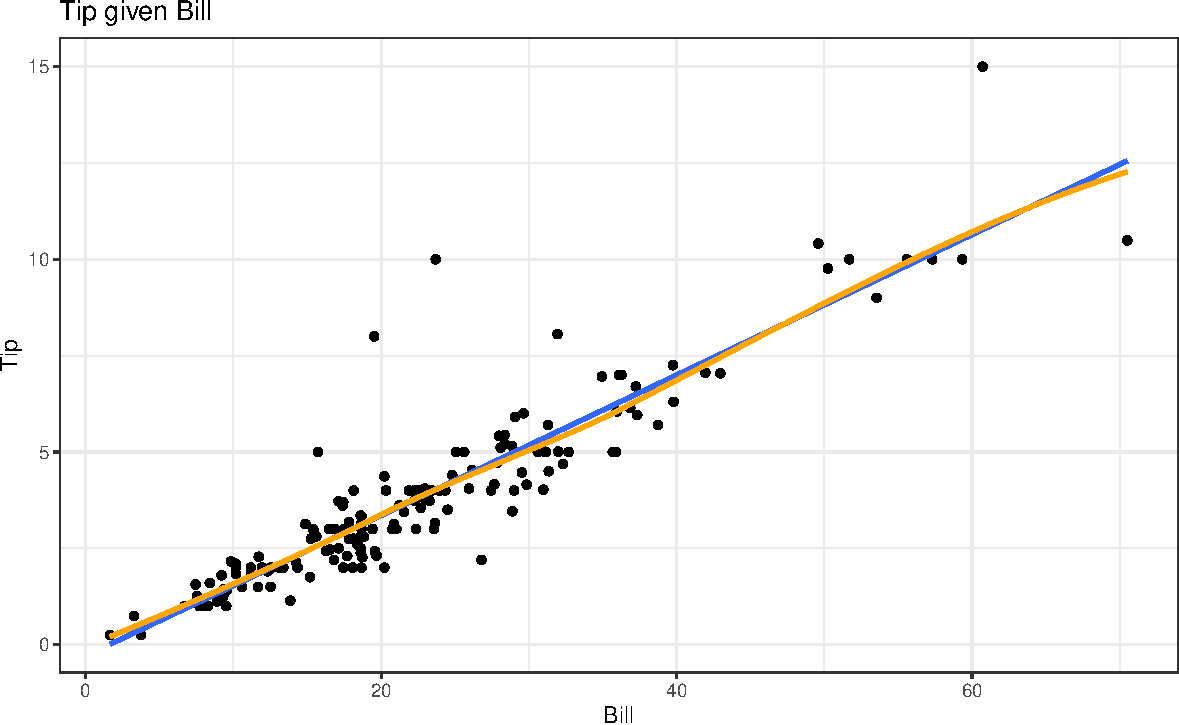
\includegraphics[width=0.7\textwidth,height=\textheight]{intro_linear_regression_files/figure-pdf/RegressionCheck-1.pdf}

}

\end{figure}

That looks pretty darn linear! There are a few unusually large tips, but
no extreme outliers, and variability appears to be constant at all
levels of \texttt{Bill} , so we proceed:

\begin{Shaded}
\begin{Highlighting}[]
\CommentTok{\# fit the linear model}
\NormalTok{mod }\OtherTok{\textless{}{-}} \FunctionTok{lm}\NormalTok{(Tip }\SpecialCharTok{\textasciitilde{}}\NormalTok{ Bill, }\AttributeTok{data =}\NormalTok{ RestaurantTips)}
\FunctionTok{summary}\NormalTok{(mod)}
\end{Highlighting}
\end{Shaded}

\begin{verbatim}

Call:
lm(formula = Tip ~ Bill, data = RestaurantTips)

Residuals:
   Min     1Q Median     3Q    Max 
-2.391 -0.489 -0.111  0.284  5.974 

Coefficients:
            Estimate Std. Error t value Pr(>|t|)    
(Intercept) -0.29227    0.16616   -1.76    0.081 .  
Bill         0.18221    0.00645   28.25   <2e-16 ***
---
Signif. codes:  0 '***' 0.001 '**' 0.01 '*' 0.05 '.' 0.1 ' ' 1

Residual standard error: 0.98 on 155 degrees of freedom
Multiple R-squared:  0.837, Adjusted R-squared:  0.836 
F-statistic:  798 on 1 and 155 DF,  p-value: <2e-16
\end{verbatim}

The first line tells R to fit the regression. The thing on the left of
the \texttt{\textasciitilde{}} is our outcome, the things on the right
are our covariates or predictors. R then saves the results of all that
work under the name \texttt{mod} (short for model - you can call it
anything you want). Once we fit the model, we used \texttt{summary()}
command to print the output to the screen.

Results relevant to the intercept are in the \texttt{(Intercept)} row
and results relevant to the slope are in the \texttt{Bill} row
(\texttt{Bill} is the explanatory variable). The \texttt{Estimate}
column gives the estimated coefficients, the \texttt{Std.\ Error} column
gives the standard error for these estimates, the \texttt{t\ value} is
simply estimate/SE, and the p-value is the result of a hypothesis test
testing whether that coefficient is significantly different from 0.

We also see the RMSE as \texttt{Residual\ standard\ error} and \(R^2\)
as \texttt{Multiple\ R-squared}. The last line of the regression output
gives details relevant to an ANOVA table for testing our model against
no model. It has the F-statistic, degrees of freedom, and p-value.

You can pull the coefficients of your model out with the \texttt{coef()}
command:

\begin{Shaded}
\begin{Highlighting}[]
\FunctionTok{coef}\NormalTok{(mod)}
\end{Highlighting}
\end{Shaded}

\begin{verbatim}
(Intercept)        Bill 
     -0.292       0.182 
\end{verbatim}

\begin{Shaded}
\begin{Highlighting}[]
\FunctionTok{coef}\NormalTok{(mod)[}\DecValTok{1}\NormalTok{] }\CommentTok{\# intercept}
\end{Highlighting}
\end{Shaded}

\begin{verbatim}
(Intercept) 
     -0.292 
\end{verbatim}

\begin{Shaded}
\begin{Highlighting}[]
\FunctionTok{coef}\NormalTok{(mod)[}\DecValTok{2}\NormalTok{] }\CommentTok{\# slope}
\end{Highlighting}
\end{Shaded}

\begin{verbatim}
 Bill 
0.182 
\end{verbatim}

\begin{Shaded}
\begin{Highlighting}[]
\FunctionTok{coef}\NormalTok{(mod)[}\StringTok{"Bill"}\NormalTok{] }\CommentTok{\# alternate way.}
\end{Highlighting}
\end{Shaded}

\begin{verbatim}
 Bill 
0.182 
\end{verbatim}

Alternatively, you can use the \texttt{tidy()} function from
\texttt{broom} to turn the regression results into a tidy data frame,
which makes it easier to work with:

\begin{Shaded}
\begin{Highlighting}[]
\FunctionTok{tidy}\NormalTok{(mod)}
\end{Highlighting}
\end{Shaded}

\begin{verbatim}
# A tibble: 2 x 5
  term        estimate std.error statistic  p.value
  <chr>          <dbl>     <dbl>     <dbl>    <dbl>
1 (Intercept)   -0.292   0.166       -1.76 8.06e- 2
2 Bill           0.182   0.00645     28.2  5.24e-63
\end{verbatim}

\begin{Shaded}
\begin{Highlighting}[]
\FunctionTok{tidy}\NormalTok{(mod)[[}\DecValTok{2}\NormalTok{,}\DecValTok{2}\NormalTok{]] }\CommentTok{\# slope}
\end{Highlighting}
\end{Shaded}

\begin{verbatim}
[1] 0.182
\end{verbatim}

We can plot our regression line on top of the scatterplot manually using
the \texttt{geom\_abline()} layer in ggplot:

\begin{Shaded}
\begin{Highlighting}[]
\FunctionTok{ggplot}\NormalTok{( RestaurantTips, }\FunctionTok{aes}\NormalTok{( Bill, Tip ) ) }\SpecialCharTok{+}
  \FunctionTok{geom\_point}\NormalTok{() }\SpecialCharTok{+}
  \FunctionTok{geom\_abline}\NormalTok{( }\AttributeTok{intercept =} \SpecialCharTok{{-}}\FloatTok{0.292}\NormalTok{, }\AttributeTok{slope =}  \FloatTok{0.182}\NormalTok{, }\AttributeTok{col=}\StringTok{"red"}\NormalTok{ )}
\end{Highlighting}
\end{Shaded}

\begin{figure}[H]

{\centering 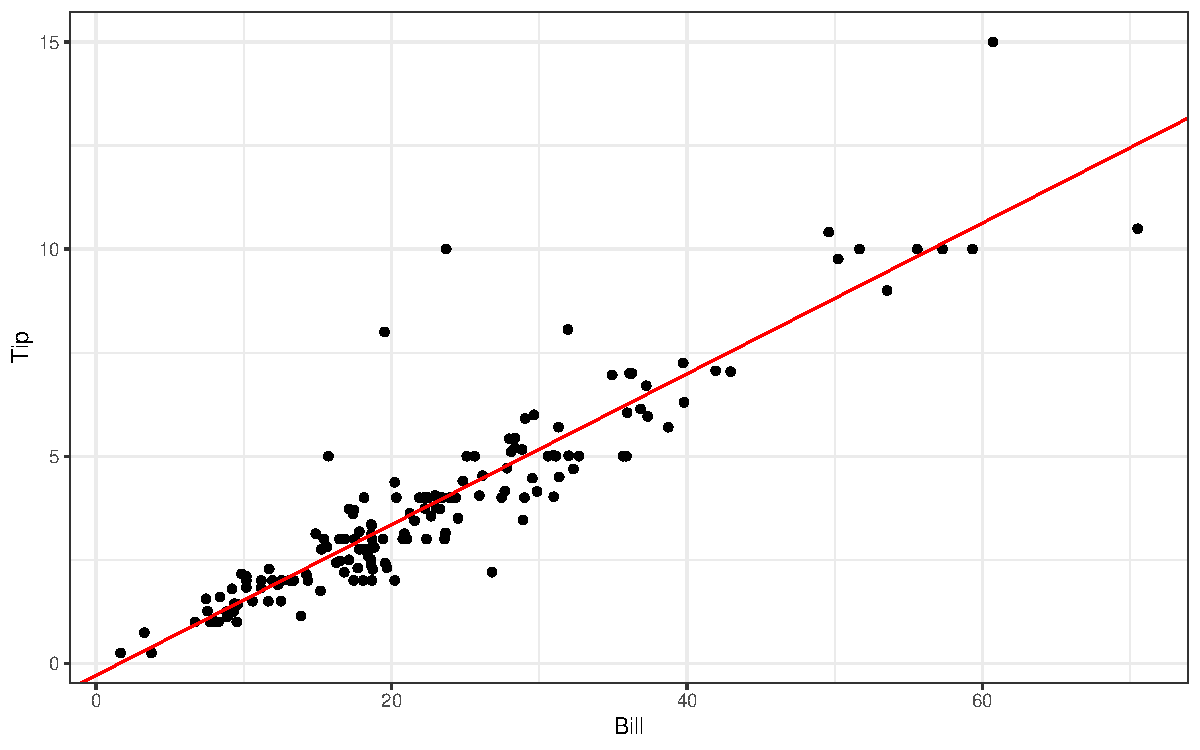
\includegraphics[width=0.7\textwidth,height=\textheight]{intro_linear_regression_files/figure-pdf/LinearRegressionPlot-1.pdf}

}

\end{figure}

\hypertarget{multiple-regression}{%
\section{Multiple Regression}\label{multiple-regression}}

We now include the additional explanatory variables of number in party
(\texttt{Guests}) and whether or not they pay with a credit card
(\texttt{Credit}):

\begin{Shaded}
\begin{Highlighting}[]
\NormalTok{tip.mod }\OtherTok{\textless{}{-}} \FunctionTok{lm}\NormalTok{(Tip }\SpecialCharTok{\textasciitilde{}}\NormalTok{ Bill }\SpecialCharTok{+}\NormalTok{ Guests }\SpecialCharTok{+}\NormalTok{ Credit, }\AttributeTok{data=}\NormalTok{RestaurantTips )}
\FunctionTok{summary}\NormalTok{(tip.mod)}
\end{Highlighting}
\end{Shaded}

\begin{verbatim}

Call:
lm(formula = Tip ~ Bill + Guests + Credit, data = RestaurantTips)

Residuals:
   Min     1Q Median     3Q    Max 
-2.384 -0.478 -0.108  0.272  5.984 

Coefficients:
            Estimate Std. Error t value Pr(>|t|)    
(Intercept) -0.25468    0.20273   -1.26     0.21    
Bill         0.18302    0.00846   21.64   <2e-16 ***
Guests      -0.03319    0.10282   -0.32     0.75    
Credity      0.04217    0.18282    0.23     0.82    
---
Signif. codes:  0 '***' 0.001 '**' 0.01 '*' 0.05 '.' 0.1 ' ' 1

Residual standard error: 0.985 on 153 degrees of freedom
Multiple R-squared:  0.838, Adjusted R-squared:  0.834 
F-statistic:  263 on 3 and 153 DF,  p-value: <2e-16
\end{verbatim}

This output should look very similar to the output for one variable,
except now there is a row corresponding to each explanatory variable.
Our two-category (y, n) \texttt{Credit} variable was automatically
converted to a 0-1 dummy variable (with ``y'' being 1 and ``n'' our
baseline).

\hypertarget{easy-tabulation-and-graphing-of-multiple-regression-models}{%
\subsection{Easy Tabulation and Graphing of Multiple Regression
Models}\label{easy-tabulation-and-graphing-of-multiple-regression-models}}

For publication-ready tables and graphics, R has many wonderful packages
to automate the process. I (JG) am partial to \texttt{tab\_model} from
\texttt{sjPlot} for regression tables, and \texttt{ggeffects} for
regression graphs, as shown below. See more in the other chapters.

\begin{Shaded}
\begin{Highlighting}[]
\CommentTok{\# tabulate the results of our two tip models}
\FunctionTok{tab\_model}\NormalTok{(mod, tip.mod)}
\end{Highlighting}
\end{Shaded}

\begin{longtable}[]{@{}ccccccc@{}}
\toprule\noalign{}
\endhead
\bottomrule\noalign{}
\endlastfoot
~ &
\multicolumn{3}{>{\centering\arraybackslash}p{(\columnwidth - 12\tabcolsep) * \real{0.0000} + 4\tabcolsep}}{%
Tip} &
\multicolumn{3}{>{\centering\arraybackslash}p{(\columnwidth - 12\tabcolsep) * \real{0.0000} + 4\tabcolsep}@{}}{%
Tip} \\
Predictors & Estimates & CI & p & Estimates & CI & p \\
(Intercept) & -0.29 & -0.62~--~0.04 & 0.081 & -0.25 & -0.66~--~0.15 &
0.211 \\
Bill & 0.18 & 0.17~--~0.19 & \textbf{\textless0.001} & 0.18 &
0.17~--~0.20 & \textbf{\textless0.001} \\
Guests & & & & -0.03 & -0.24~--~0.17 & 0.747 \\
Credit {[}y{]} & & & & 0.04 & -0.32~--~0.40 & 0.818 \\
Observations &
\multicolumn{3}{>{\raggedright\arraybackslash}p{(\columnwidth - 12\tabcolsep) * \real{0.0000} + 4\tabcolsep}}{%
157} &
\multicolumn{3}{>{\raggedright\arraybackslash}p{(\columnwidth - 12\tabcolsep) * \real{0.0000} + 4\tabcolsep}@{}}{%
157} \\
R\textsuperscript{2} / R\textsuperscript{2} adjusted &
\multicolumn{3}{>{\raggedright\arraybackslash}p{(\columnwidth - 12\tabcolsep) * \real{0.0000} + 4\tabcolsep}}{%
0.837 / 0.836} &
\multicolumn{3}{>{\raggedright\arraybackslash}p{(\columnwidth - 12\tabcolsep) * \real{0.0000} + 4\tabcolsep}@{}}{%
0.838 / 0.834} \\
\end{longtable}

\begin{Shaded}
\begin{Highlighting}[]
\CommentTok{\# graph model 2, with Bill on X, Credit as color, and Guests held constant at the mean}
\FunctionTok{ggeffect}\NormalTok{(tip.mod, }\AttributeTok{terms =} \FunctionTok{c}\NormalTok{(}\StringTok{"Bill"}\NormalTok{, }\StringTok{"Credit"}\NormalTok{)) }\SpecialCharTok{|\textgreater{}} 
  \FunctionTok{plot}\NormalTok{(}\AttributeTok{add.data =} \ConstantTok{TRUE}\NormalTok{, }\AttributeTok{ci =} \ConstantTok{FALSE}\NormalTok{)}
\end{Highlighting}
\end{Shaded}

\begin{figure}[H]

{\centering \includegraphics[width=0.7\textwidth,height=\textheight]{intro_linear_regression_files/figure-pdf/unnamed-chunk-3-1.pdf}

}

\end{figure}

\hypertarget{categorical-variables-and-factors}{%
\section{Categorical Variables (and
Factors)}\label{categorical-variables-and-factors}}

You can include any explanatory categorical variable in a multiple
regression model, and R will automatically create corresponding 0/1
variables. For example, if you were to include gender coded as
male/female, R would create a variable GenderMale that is 1 for males
and 0 for females.

\hypertarget{numbers-coding-categories.}{%
\subsection{Numbers Coding
Categories.}\label{numbers-coding-categories.}}

If you have multiple levels of a category, but your levels are coded
with numbers you have to be a bit careful because R can treat this as a
quantitative (continuous) variable by mistake in some cases. You will
know it did this if you only see the single variable on one line of your
output. For categorical variables with \(k\) categories, you should see
\(k-1\) lines.

To make a variable categorical, even if the levels are numbers, convert
the variable to a factor with \texttt{as.factor} or \texttt{factor}:

\begin{Shaded}
\begin{Highlighting}[]
\CommentTok{\# load the US states data}
\FunctionTok{data}\NormalTok{( USStates )}

\CommentTok{\# convert Region to a factor}
\NormalTok{USStates }\OtherTok{\textless{}{-}}\NormalTok{ USStates }\SpecialCharTok{|\textgreater{}} 
  \FunctionTok{mutate}\NormalTok{(}\AttributeTok{Region =} \FunctionTok{factor}\NormalTok{(Region))}
\end{Highlighting}
\end{Shaded}

\hypertarget{setting-new-baselines.}{%
\subsection{Setting new baselines.}\label{setting-new-baselines.}}

We can reorder the levels if desired (the first is our baseline).

\begin{Shaded}
\begin{Highlighting}[]
\FunctionTok{levels}\NormalTok{( USStates}\SpecialCharTok{$}\NormalTok{Region )}
\end{Highlighting}
\end{Shaded}

\begin{verbatim}
[1] "MW" "NE" "S"  "W" 
\end{verbatim}

\begin{Shaded}
\begin{Highlighting}[]
\NormalTok{USStates}\SpecialCharTok{$}\NormalTok{Region }\OtherTok{=} \FunctionTok{relevel}\NormalTok{(USStates}\SpecialCharTok{$}\NormalTok{Region, }\StringTok{"S"}\NormalTok{ )}
\FunctionTok{levels}\NormalTok{( USStates}\SpecialCharTok{$}\NormalTok{Region )}
\end{Highlighting}
\end{Shaded}

\begin{verbatim}
[1] "S"  "MW" "NE" "W" 
\end{verbatim}

Now any regression will use the south as baseline.

\hypertarget{testing-for-significance-of-a-categorical-variable.}{%
\subsection{Testing for significance of a categorical
variable.}\label{testing-for-significance-of-a-categorical-variable.}}

When deciding whether to keep a categorical variable, we need to test
how important all the dummy variables for that category are to the model
all at once. We do this with ANOVA. Here we examine whether region is
useful for predicting the percent vote for Clinton in 2016:

\begin{Shaded}
\begin{Highlighting}[]
\NormalTok{mlm }\OtherTok{=} \FunctionTok{lm}\NormalTok{( ClintonVote }\SpecialCharTok{\textasciitilde{}}\NormalTok{ Region, }\AttributeTok{data=}\NormalTok{USStates)}
\FunctionTok{anova}\NormalTok{( mlm )}
\end{Highlighting}
\end{Shaded}

\begin{verbatim}
Analysis of Variance Table

Response: ClintonVote
          Df Sum Sq Mean Sq F value  Pr(>F)    
Region     3   1643     548    6.99 0.00057 ***
Residuals 46   3603      78                    
---
Signif. codes:  0 '***' 0.001 '**' 0.01 '*' 0.05 '.' 0.1 ' ' 1
\end{verbatim}

It is quite important.

We can also compare for region beyond some other variable:

\begin{Shaded}
\begin{Highlighting}[]
\NormalTok{mlm2 }\OtherTok{=} \FunctionTok{lm}\NormalTok{( ClintonVote }\SpecialCharTok{\textasciitilde{}}\NormalTok{ HouseholdIncome }\SpecialCharTok{+}\NormalTok{ HouseholdIncome }\SpecialCharTok{+}\NormalTok{ HighSchool }\SpecialCharTok{+} 
\NormalTok{               EighthGradeMath, }\AttributeTok{data=}\NormalTok{USStates)}

\NormalTok{mlm3 }\OtherTok{=} \FunctionTok{lm}\NormalTok{( ClintonVote }\SpecialCharTok{\textasciitilde{}}\NormalTok{ HouseholdIncome }\SpecialCharTok{+}\NormalTok{ HouseholdIncome }\SpecialCharTok{+}\NormalTok{ HighSchool }\SpecialCharTok{+} 
\NormalTok{               EighthGradeMath }\SpecialCharTok{+}\NormalTok{ Region, }\AttributeTok{data=}\NormalTok{USStates)}
\FunctionTok{anova}\NormalTok{( mlm2, mlm3 )}
\end{Highlighting}
\end{Shaded}

\begin{verbatim}
Analysis of Variance Table

Model 1: ClintonVote ~ HouseholdIncome + HouseholdIncome + HighSchool + 
    EighthGradeMath
Model 2: ClintonVote ~ HouseholdIncome + HouseholdIncome + HighSchool + 
    EighthGradeMath + Region
  Res.Df  RSS Df Sum of Sq    F Pr(>F)  
1     46 3287                           
2     43 2649  3       638 3.45  0.025 *
---
Signif. codes:  0 '***' 0.001 '**' 0.01 '*' 0.05 '.' 0.1 ' ' 1
\end{verbatim}

Region is still important, beyond including some further controls.
Interpreting this mess of a regression is not part of this document;
this document shows you how to run regressions but it doesn't discuss
whether you should or not.

\hypertarget{missing-levels-in-a-factor}{%
\subsection{Missing levels in a
factor}\label{missing-levels-in-a-factor}}

R often treats categorical variables as factors. This is often useful,
but sometimes annoying. A factor has different \textbf{levels} which are
the different values it can be. For example:

\begin{Shaded}
\begin{Highlighting}[]
\FunctionTok{data}\NormalTok{(FishGills3)}
\FunctionTok{levels}\NormalTok{(FishGills3}\SpecialCharTok{$}\NormalTok{Calcium)}
\end{Highlighting}
\end{Shaded}

\begin{verbatim}
[1] ""       "High"   "Low"    "Medium"
\end{verbatim}

\begin{Shaded}
\begin{Highlighting}[]
\FunctionTok{table}\NormalTok{(FishGills3}\SpecialCharTok{$}\NormalTok{Calcium)}
\end{Highlighting}
\end{Shaded}

\begin{verbatim}

         High    Low Medium 
     0     30     30     30 
\end{verbatim}

Note the weird nameless level; it also has no actual observations in it.
Nevertheless, if you make a boxplot, you will get an empty plot in
addition to the other three. This error was likely due to some past data
entry issue. You can drop the unused level:

\begin{Shaded}
\begin{Highlighting}[]
\NormalTok{FishGills3}\SpecialCharTok{$}\NormalTok{Calcium }\OtherTok{=} \FunctionTok{droplevels}\NormalTok{(FishGills3}\SpecialCharTok{$}\NormalTok{Calcium)}
\end{Highlighting}
\end{Shaded}

You can also turn a categorical variable into a numeric one like so:

\begin{Shaded}
\begin{Highlighting}[]
\FunctionTok{summary}\NormalTok{( FishGills3}\SpecialCharTok{$}\NormalTok{Calcium )}
\end{Highlighting}
\end{Shaded}

\begin{verbatim}
  High    Low Medium 
    30     30     30 
\end{verbatim}

\begin{Shaded}
\begin{Highlighting}[]
\NormalTok{asnum }\OtherTok{=} \FunctionTok{as.numeric}\NormalTok{( FishGills3}\SpecialCharTok{$}\NormalTok{Calcium )}
\NormalTok{asnum}
\end{Highlighting}
\end{Shaded}

\begin{verbatim}
 [1] 2 2 2 2 2 2 2 2 2 2 2 2 2 2 2 2 2 2 2 2 2 2 2 2 2 2 2 2 2 2 3 3 3 3 3 3 3 3
[39] 3 3 3 3 3 3 3 3 3 3 3 3 3 3 3 3 3 3 3 3 3 3 1 1 1 1 1 1 1 1 1 1 1 1 1 1 1 1
[77] 1 1 1 1 1 1 1 1 1 1 1 1 1 1
\end{verbatim}

Regression on only a categorical variable is fine:

\begin{Shaded}
\begin{Highlighting}[]
\NormalTok{mylm }\OtherTok{=} \FunctionTok{lm}\NormalTok{( GillRate }\SpecialCharTok{\textasciitilde{}}\NormalTok{ Calcium, }\AttributeTok{data=}\NormalTok{FishGills3 )}
\NormalTok{mylm}
\end{Highlighting}
\end{Shaded}

\begin{verbatim}

Call:
lm(formula = GillRate ~ Calcium, data = FishGills3)

Coefficients:
  (Intercept)     CalciumLow  CalciumMedium  
         58.2           10.3            0.5  
\end{verbatim}

R has made you a bunch of dummy variables automatically. Here ``high''
is the baseline, selected automatically. We can also force it so there
is no baseline by removing the intercept, in which case the coefficients
are the means of each group.

\begin{Shaded}
\begin{Highlighting}[]
\NormalTok{mymm }\OtherTok{=} \FunctionTok{lm}\NormalTok{( GillRate }\SpecialCharTok{\textasciitilde{}} \DecValTok{0} \SpecialCharTok{+}\NormalTok{ Calcium, }\AttributeTok{data=}\NormalTok{FishGills3 )}
\NormalTok{mymm}
\end{Highlighting}
\end{Shaded}

\begin{verbatim}

Call:
lm(formula = GillRate ~ 0 + Calcium, data = FishGills3)

Coefficients:
  CalciumHigh     CalciumLow  CalciumMedium  
         58.2           68.5           58.7  
\end{verbatim}

\hypertarget{some-extra-stuff-optional}{%
\section{Some extra stuff (optional)}\label{some-extra-stuff-optional}}

\hypertarget{confidence-intervals}{%
\subsection{Confidence Intervals}\label{confidence-intervals}}

To get confidence intervals around each parameter in your model, try
this:

\begin{Shaded}
\begin{Highlighting}[]
\FunctionTok{confint}\NormalTok{(tip.mod)}
\end{Highlighting}
\end{Shaded}

\begin{verbatim}
             2.5 % 97.5 %
(Intercept) -0.655  0.146
Bill         0.166  0.200
Guests      -0.236  0.170
Credity     -0.319  0.403
\end{verbatim}

You can also create them easily using \texttt{tidy} and \texttt{mutate}:

\begin{Shaded}
\begin{Highlighting}[]
\NormalTok{tip.mod }\SpecialCharTok{|\textgreater{}} 
  \FunctionTok{tidy}\NormalTok{() }\SpecialCharTok{|\textgreater{}} 
  \FunctionTok{mutate}\NormalTok{(}\AttributeTok{upper =}\NormalTok{ estimate }\SpecialCharTok{+} \FloatTok{1.96}\SpecialCharTok{*}\NormalTok{std.error,}
         \AttributeTok{lower =}\NormalTok{ estimate }\SpecialCharTok{{-}} \FloatTok{1.96}\SpecialCharTok{*}\NormalTok{std.error)}
\end{Highlighting}
\end{Shaded}

\begin{verbatim}
# A tibble: 4 x 7
  term        estimate std.error statistic  p.value upper  lower
  <chr>          <dbl>     <dbl>     <dbl>    <dbl> <dbl>  <dbl>
1 (Intercept)  -0.255    0.203      -1.26  2.11e- 1 0.143 -0.652
2 Bill          0.183    0.00846    21.6   2.07e-48 0.200  0.166
3 Guests       -0.0332   0.103      -0.323 7.47e- 1 0.168 -0.235
4 Credity       0.0422   0.183       0.231 8.18e- 1 0.400 -0.316
\end{verbatim}

\hypertarget{prediction}{%
\subsection{Prediction}\label{prediction}}

Suppose a server at this bistro is about to deliver a \$20 bill, and
wants to predict their tip. They can get a predicted value and 95\%
(this is the default level, change with level) prediction interval with

\begin{Shaded}
\begin{Highlighting}[]
\NormalTok{new.dat }\OtherTok{=} \FunctionTok{data.frame}\NormalTok{( }\AttributeTok{Bill =} \FunctionTok{c}\NormalTok{(}\DecValTok{20}\NormalTok{) )}
\FunctionTok{predict}\NormalTok{(mod,new.dat,}\AttributeTok{interval =} \StringTok{"prediction"}\NormalTok{)}
\end{Highlighting}
\end{Shaded}

\begin{verbatim}
   fit  lwr  upr
1 3.35 1.41 5.29
\end{verbatim}

They should expect a tip somewhere between \$1.41 and \$5.30.

If we know a bit more we can use our more complex model called
\texttt{tip.mod} from above:

\begin{Shaded}
\begin{Highlighting}[]
\NormalTok{new.dat }\OtherTok{=} \FunctionTok{data.frame}\NormalTok{( }\AttributeTok{Bill =} \FunctionTok{c}\NormalTok{(}\DecValTok{20}\NormalTok{), }\AttributeTok{Guests=}\FunctionTok{c}\NormalTok{(}\DecValTok{1}\NormalTok{), }\AttributeTok{Credit=}\FunctionTok{c}\NormalTok{(}\StringTok{"n"}\NormalTok{) )}
\FunctionTok{predict}\NormalTok{(tip.mod,new.dat,}\AttributeTok{interval =} \StringTok{"prediction"}\NormalTok{)}
\end{Highlighting}
\end{Shaded}

\begin{verbatim}
   fit  lwr  upr
1 3.37 1.41 5.34
\end{verbatim}

This is the predicted tip for one guest paying with cash for a \$20 tip.
It is wider than our original interval because our model is a bit more
unstable (it turns out guest number and credit card aren't that relevant
or helpful).

Compare the prediction interval to the confidence interval

\begin{Shaded}
\begin{Highlighting}[]
\NormalTok{new.dat }\OtherTok{=} \FunctionTok{data.frame}\NormalTok{( }\AttributeTok{Bill =} \FunctionTok{c}\NormalTok{(}\DecValTok{20}\NormalTok{), }\AttributeTok{Guests=}\FunctionTok{c}\NormalTok{(}\DecValTok{1}\NormalTok{), }\AttributeTok{Credit=}\FunctionTok{c}\NormalTok{(}\StringTok{"n"}\NormalTok{) )}
\FunctionTok{predict}\NormalTok{(tip.mod, new.dat, }\AttributeTok{interval =} \StringTok{"confidence"}\NormalTok{)}
\end{Highlighting}
\end{Shaded}

\begin{verbatim}
   fit  lwr  upr
1 3.37 3.09 3.65
\end{verbatim}

This predicts the mean tip for all single guests who pay a \$20 bill
with cash. Our interval is smaller because we are generating a
confidence interval for where the mean is, and are ignoring that
individuals will vary around that mean. Confidence intervals are
different from prediction intervals.

\hypertarget{removing-outliers}{%
\subsection{Removing Outliers}\label{removing-outliers}}

If you can identify which rows the outliers are on, you can do this by
hand (say the rows are 5, 10, 12).

\begin{Shaded}
\begin{Highlighting}[]
\NormalTok{new.data }\OtherTok{=}\NormalTok{ old.data[ }\SpecialCharTok{{-}}\FunctionTok{c}\NormalTok{(}\DecValTok{5}\NormalTok{,}\DecValTok{10}\NormalTok{,}\DecValTok{12}\NormalTok{), ]}
\FunctionTok{lm}\NormalTok{( Y }\SpecialCharTok{\textasciitilde{}}\NormalTok{ X, }\AttributeTok{data=}\NormalTok{new.data )}
\end{Highlighting}
\end{Shaded}

Some technical details: The \texttt{c(5,10,12)} is a list of 3 numbers.
The \texttt{c()} is the concatenation function that takes things makes
lists out of them. The ``-list'' notation means give me my old data, but
without rows 5, 10, and 12. Note the comma after the list. This is
because we identify elements in a dataframe with row, column notation.
So \texttt{old.data{[}1,3{]}} would be row 1, column 3.

If you notice your points all have X bigger than some value, say 20.5,
you could use filtering to keep everything less than some value:

\begin{Shaded}
\begin{Highlighting}[]
\NormalTok{new.data }\OtherTok{=} \FunctionTok{filter}\NormalTok{( old.data, X }\SpecialCharTok{\textless{}=} \FloatTok{20.5}\NormalTok{ )}
\end{Highlighting}
\end{Shaded}

\hypertarget{missing-data}{%
\subsection{Missing data}\label{missing-data}}

If you have missing data, \texttt{lm} will automatically drop those
cases because it doesn't know what else to do. It will tell you this,
however, with the \texttt{summary} command.

\begin{Shaded}
\begin{Highlighting}[]
\FunctionTok{data}\NormalTok{(AllCountries)}
\NormalTok{dev.lm }\OtherTok{=} \FunctionTok{lm}\NormalTok{( BirthRate }\SpecialCharTok{\textasciitilde{}}\NormalTok{ Rural }\SpecialCharTok{+}\NormalTok{ Health }\SpecialCharTok{+}\NormalTok{ ElderlyPop, }\AttributeTok{data=}\NormalTok{AllCountries )}
\FunctionTok{summary}\NormalTok{( dev.lm  )}
\end{Highlighting}
\end{Shaded}

\begin{verbatim}

Call:
lm(formula = BirthRate ~ Rural + Health + ElderlyPop, data = AllCountries)

Residuals:
    Min      1Q  Median      3Q     Max 
-16.592  -3.728  -0.791   3.909  16.218 

Coefficients:
            Estimate Std. Error t value Pr(>|t|)    
(Intercept)  26.5763     1.6795   15.82  < 2e-16 ***
Rural         0.0985     0.0224    4.40  1.9e-05 ***
Health       -0.0995     0.0930   -1.07     0.29    
ElderlyPop   -1.0249     0.0881  -11.64  < 2e-16 ***
---
Signif. codes:  0 '***' 0.001 '**' 0.01 '*' 0.05 '.' 0.1 ' ' 1

Residual standard error: 5.83 on 174 degrees of freedom
  (39 observations deleted due to missingness)
Multiple R-squared:  0.663, Adjusted R-squared:  0.657 
F-statistic:  114 on 3 and 174 DF,  p-value: <2e-16
\end{verbatim}

\hypertarget{residual-plots-and-model-fit}{%
\subsection{Residual plots and model
fit}\label{residual-plots-and-model-fit}}

If we throw out model into the \texttt{plot} function, we get some nice
regression diagnostics.

\begin{Shaded}
\begin{Highlighting}[]
\FunctionTok{plot}\NormalTok{(tip.mod)}
\end{Highlighting}
\end{Shaded}

\begin{figure}[H]

{\centering 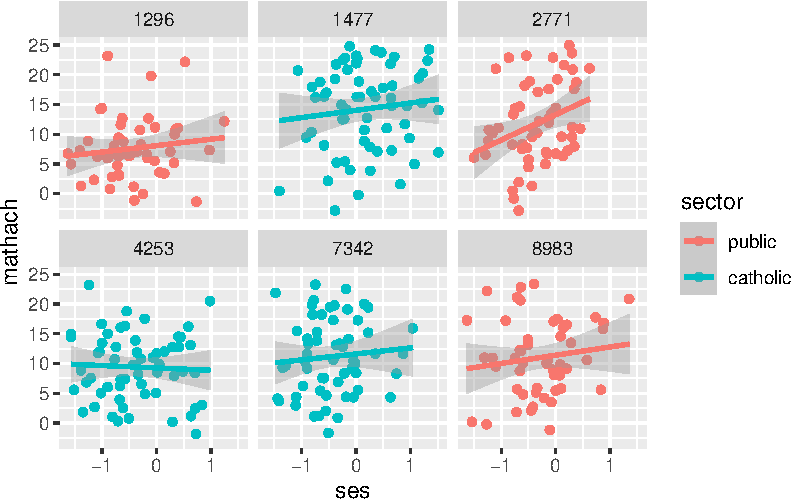
\includegraphics[width=0.7\textwidth,height=\textheight]{intro_linear_regression_files/figure-pdf/unnamed-chunk-8-1.pdf}

}

\end{figure}

\begin{figure}[H]

{\centering 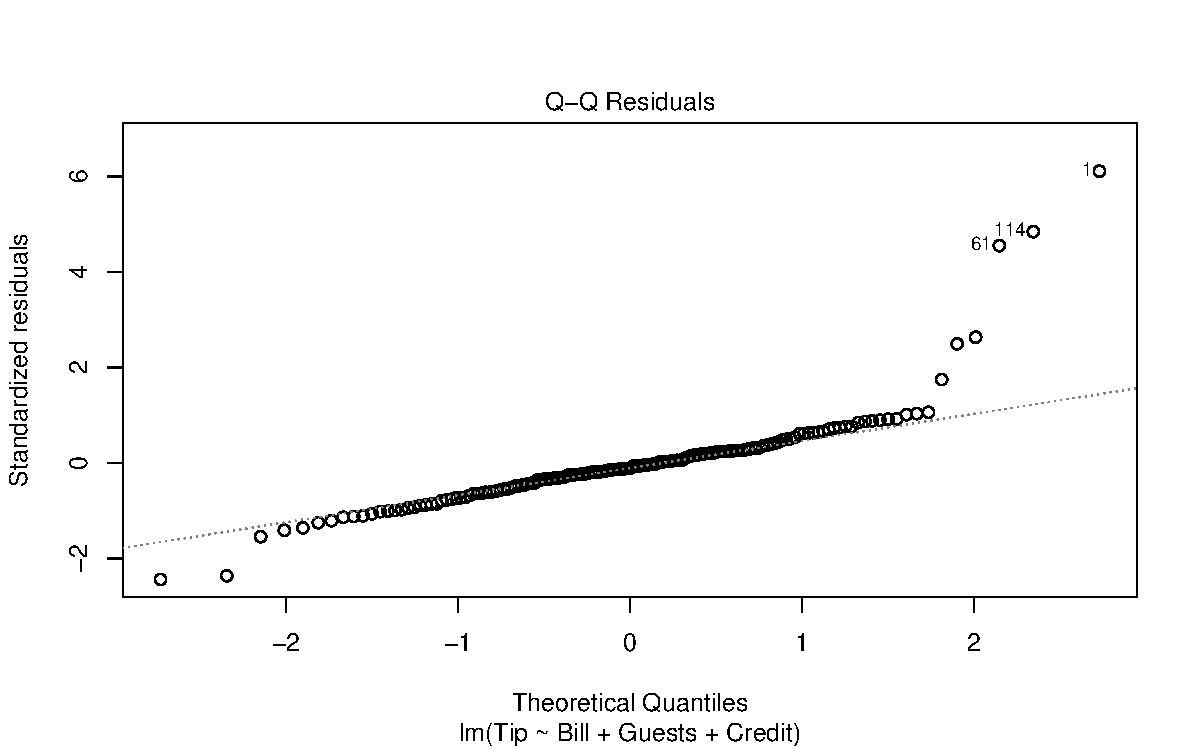
\includegraphics[width=0.7\textwidth,height=\textheight]{intro_linear_regression_files/figure-pdf/unnamed-chunk-8-2.pdf}

}

\end{figure}

\begin{figure}[H]

{\centering 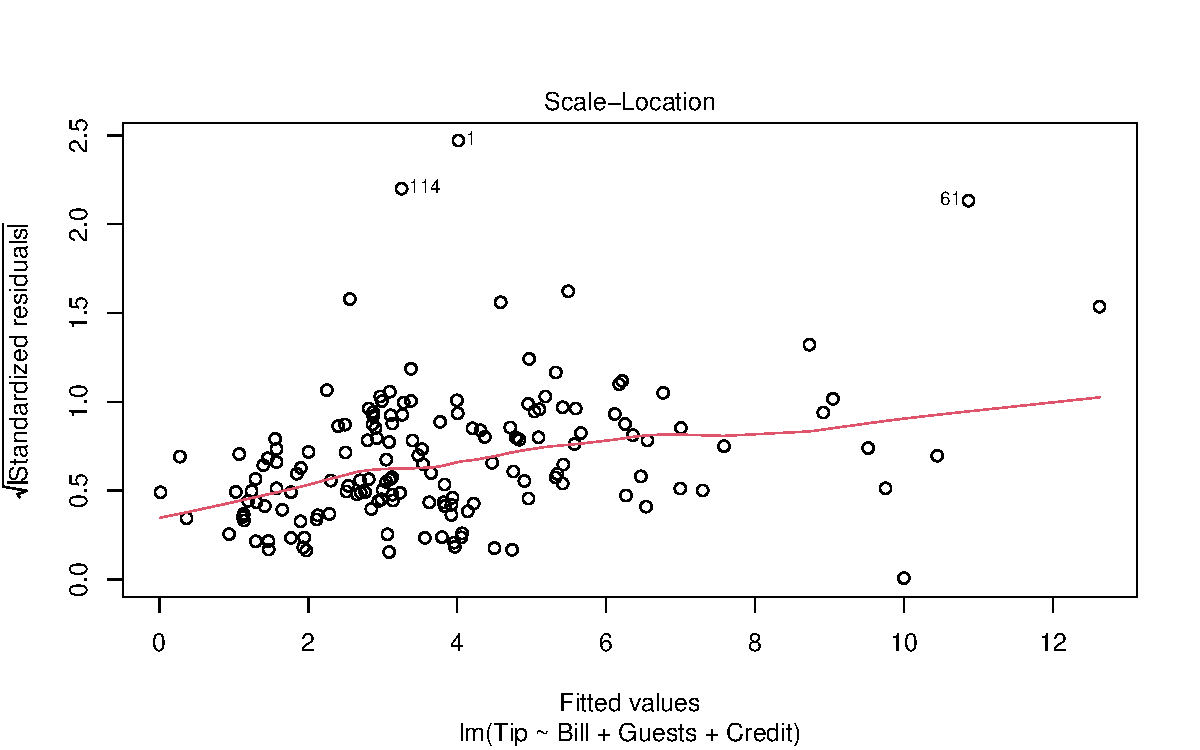
\includegraphics[width=0.7\textwidth,height=\textheight]{intro_linear_regression_files/figure-pdf/unnamed-chunk-8-3.pdf}

}

\end{figure}

\begin{figure}[H]

{\centering 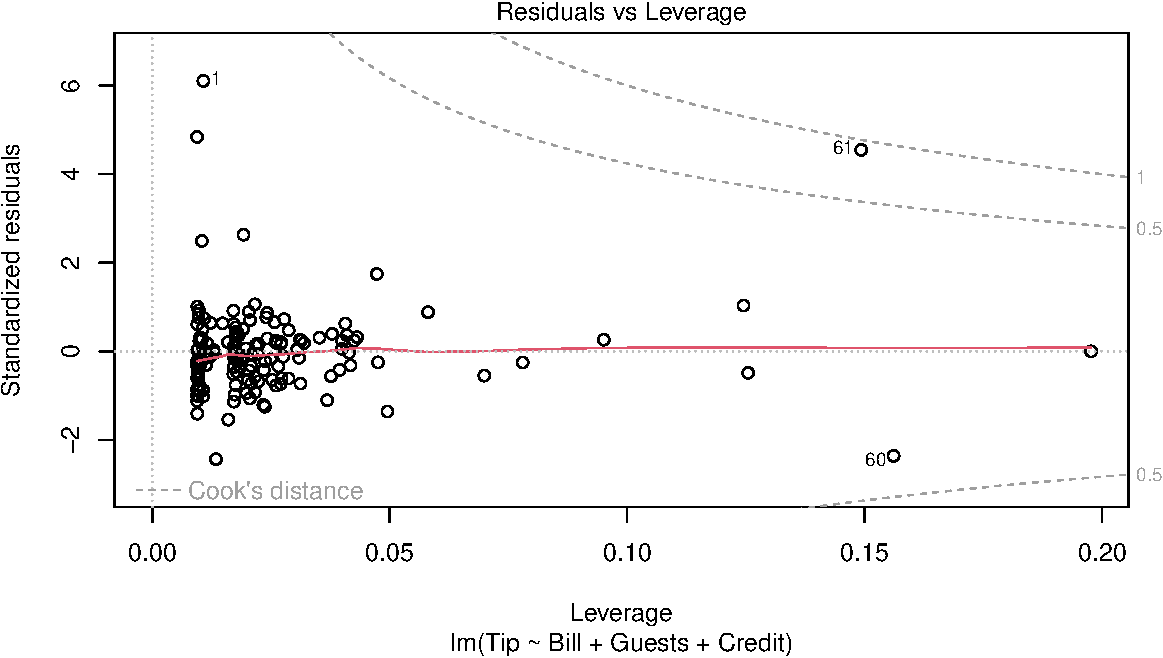
\includegraphics[width=0.7\textwidth,height=\textheight]{intro_linear_regression_files/figure-pdf/unnamed-chunk-8-4.pdf}

}

\end{figure}

To generate classic model fit diagnostics with more control, we need to
calculate residuals, make a residual versus fitted values plot, and make
a histogram of the residuals. We can make some quick and dirty plots
with \texttt{qplot} (standing for ``quick plot'') like so:

\begin{Shaded}
\begin{Highlighting}[]
\FunctionTok{qplot}\NormalTok{(tip.mod}\SpecialCharTok{$}\NormalTok{fit, tip.mod}\SpecialCharTok{$}\NormalTok{residuals )}
\end{Highlighting}
\end{Shaded}

\begin{verbatim}
Warning: `qplot()` was deprecated in ggplot2 3.4.0.
\end{verbatim}

\begin{figure}[H]

{\centering 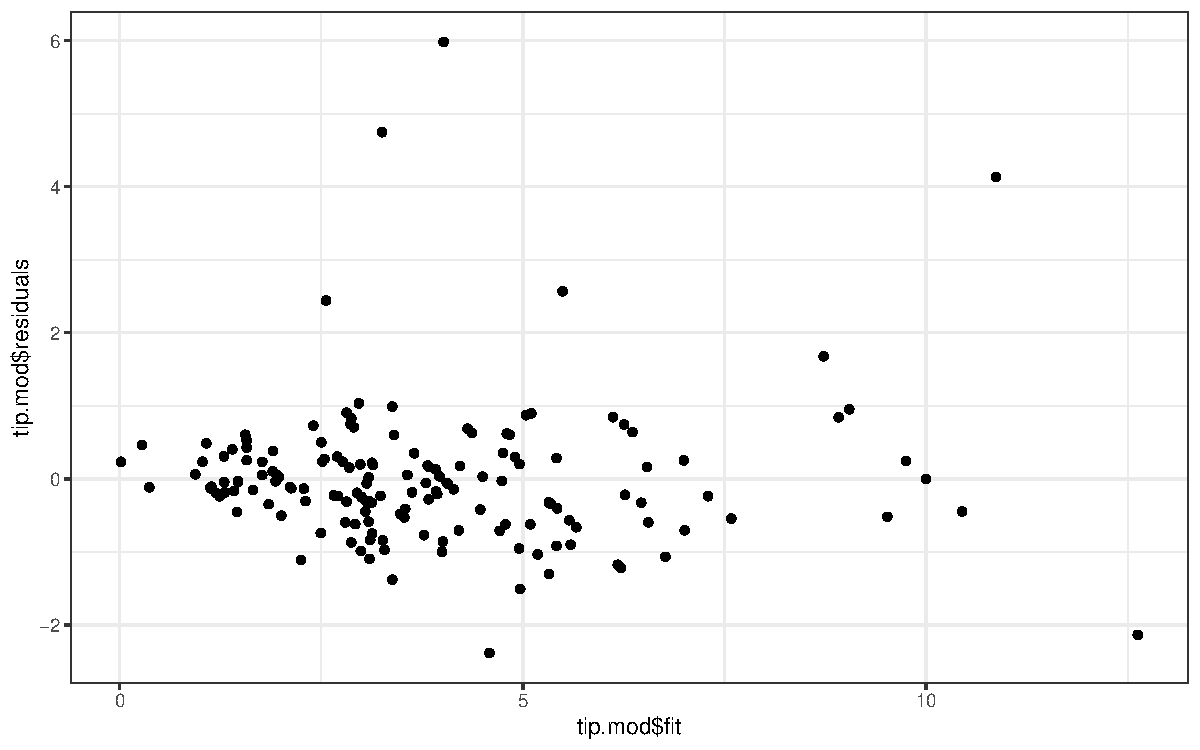
\includegraphics[width=0.7\textwidth,height=\textheight]{intro_linear_regression_files/figure-pdf/ConditionsForRegression-1.pdf}

}

\end{figure}

and

\begin{Shaded}
\begin{Highlighting}[]
\FunctionTok{qplot}\NormalTok{(tip.mod}\SpecialCharTok{$}\NormalTok{residuals, }\AttributeTok{bins=}\DecValTok{30}\NormalTok{)}
\end{Highlighting}
\end{Shaded}

\begin{figure}[H]

{\centering \includegraphics[width=0.7\textwidth,height=\textheight]{intro_linear_regression_files/figure-pdf/unnamed-chunk-9-1.pdf}

}

\end{figure}

We see no real pattern other than some extreme outliers. The residual
histogram suggests we are not really normally distributed, so we should
treat our SEs and \(p\)-values with caution. These plots are the
canonical ``model-checking'\,' plots you might use.

Another is the ``fitted outcomes vs.~actual outcomes'\,' plot of:

\begin{Shaded}
\begin{Highlighting}[]
\NormalTok{predicted }\OtherTok{=} \FunctionTok{predict}\NormalTok{( dev.lm )}
\NormalTok{actual }\OtherTok{=}\NormalTok{ dev.lm}\SpecialCharTok{$}\NormalTok{model}\SpecialCharTok{$}\NormalTok{BirthRate}
\FunctionTok{qplot}\NormalTok{( actual, predicted, }\AttributeTok{main=}\StringTok{"Fit vs. actual Birth Rate"}\NormalTok{ )}
\end{Highlighting}
\end{Shaded}

\begin{figure}[H]

{\centering 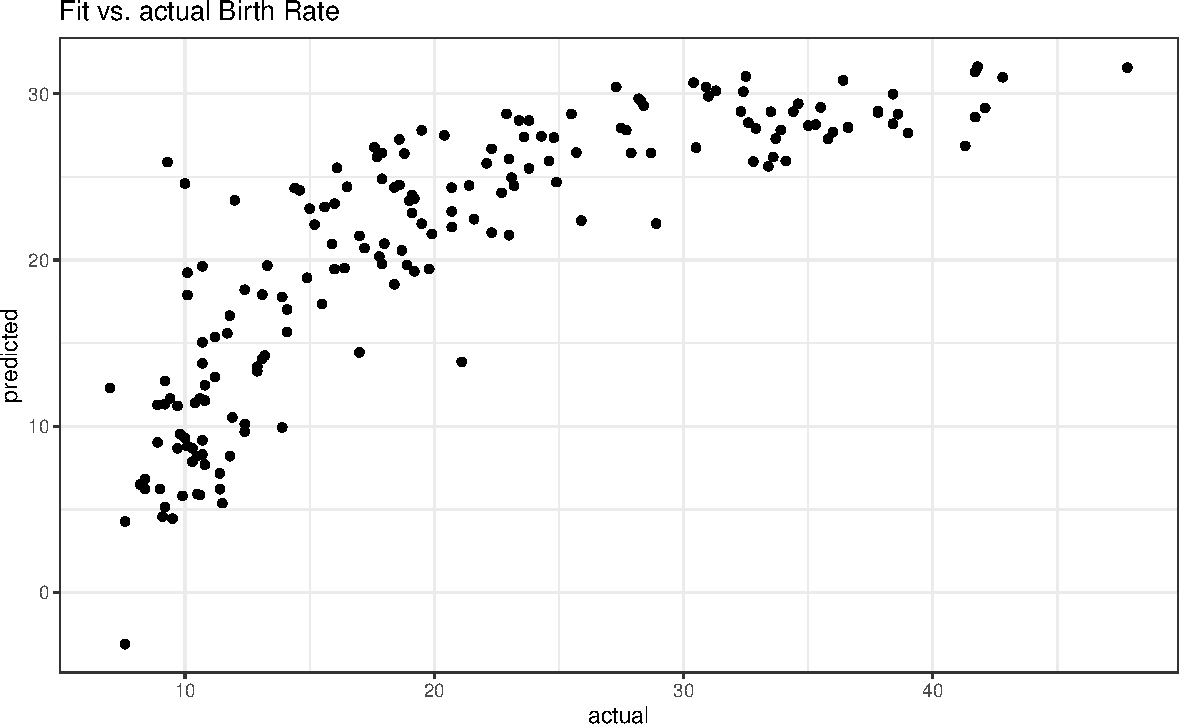
\includegraphics[width=0.7\textwidth,height=\textheight]{intro_linear_regression_files/figure-pdf/ConditionsForRegression2-1.pdf}

}

\end{figure}

Note the \texttt{dev.lm} variable has a \texttt{model} variable inside
it. This is a data frame of the \textbf{used} data for the model (i.e.,
if cases were dropped due to missingness, they will not be in the
model). We then grab the birth rates from this, and make a scatterplot.
If we tried to skip this, and use the original data, we would get an
error because our original data set has some observations that were
dropped.

Note we can't just add our predictions to \texttt{AllCountries} since we
would get an error due to this dropped data issue:

\begin{Shaded}
\begin{Highlighting}[]
\NormalTok{AllCountries}\SpecialCharTok{$}\NormalTok{predicted }\OtherTok{=} \FunctionTok{predict}\NormalTok{( dev.lm )}
\end{Highlighting}
\end{Shaded}

\begin{verbatim}
Error in `$<-.data.frame`(`*tmp*`, predicted, value = c(`1` = 31.630301617421,  : 
  replacement has 179 rows, data has 217
\end{verbatim}

We can, however, predict like this:

\begin{Shaded}
\begin{Highlighting}[]
\NormalTok{AllCountries}\SpecialCharTok{$}\NormalTok{predicted }\OtherTok{=} \FunctionTok{predict}\NormalTok{( dev.lm, }\AttributeTok{newdata=}\NormalTok{AllCountries )}
\end{Highlighting}
\end{Shaded}

The \texttt{newdata} tells predict to generate a prediction for each row
in AllCountries rather than each row in the left over data after
\texttt{lm} dropped cases with missing values.

\hypertarget{tips-tricks-and-debugging-in-r}{%
\chapter{Tips, Tricks, and Debugging in
R}\label{tips-tricks-and-debugging-in-r}}

This chapter is a complete hodge-podge of section covers ways of dealing
with data, especially messy data you might have for final projects.

\hypertarget{some-miscellaneous-advice}{%
\section{Some miscellaneous advice}\label{some-miscellaneous-advice}}

So you are starting to learn R. But there's lots of good tricks you'll
never know about until somebody shows you. Clean code is one such good
trick; consider the following: ``Your most important collaborator is you
from 6 months ago. Unfortunately, you can't ask that-you any questions,
because they don't answer their email.''

In this section we give a few things that you may find useful, either
now or later.

\hypertarget{a-few-random-tips}{%
\subsection{A few random tips}\label{a-few-random-tips}}

The letter ``l'' looks like the number ``1''---watch out for that.
Things like ``mylm'' are usually all letters, with ``lm'' standing for
linear model.

\hypertarget{quick-tips-regarding-r-markdown-report-generation}{%
\subsection{Quick tips regarding R Markdown report
generation}\label{quick-tips-regarding-r-markdown-report-generation}}

Don't put ``View()'' in your Markdown file when loading your csv file.
Just put in the \texttt{read\_csv} line. Otherwise you will not be able
to knit.

If you can't knit PDFs you need to install latex (tex). Once you do,
reboot your computer. If things don't work, then knit to Microsoft word
(or, failing that, html as a last resort), print to pdf, and turn that
in. But then ask a teaching fellow to help get things set up, since PDFs
make for much more readable reports.

\hypertarget{saving-r-objects}{%
\subsection{Saving R objects}\label{saving-r-objects}}

If you have the result of something that took awhile to run (e.g., a big
multilevel model fit to a lot of data) you can try saving it like so:

\begin{Shaded}
\begin{Highlighting}[]
\NormalTok{myBigThing }\OtherTok{=} \FunctionTok{lm}\NormalTok{(mpg }\SpecialCharTok{\textasciitilde{}}\NormalTok{ disp, }\AttributeTok{data=}\NormalTok{mtcars) }\CommentTok{\#something slow}
\FunctionTok{saveRDS}\NormalTok{(myBigThing, savedPath)}

\DocumentationTok{\#\# Later on:}
\NormalTok{myBigThing }\OtherTok{\textless{}{-}} \FunctionTok{readRDS}\NormalTok{(savedPath)}
\end{Highlighting}
\end{Shaded}

\hypertarget{r-style-based-on-google-style-guide}{%
\subsection{R style (based on Google style
guide)}\label{r-style-based-on-google-style-guide}}

Try to do the following

\begin{itemize}
\tightlist
\item
  Comment your code!
\item
  Structure of an R file:

  \begin{itemize}
  \tightlist
  \item
    Descriptive comments (including date)
  \item
    Load libraries
  \item
    Constants and script parameters (\# iterations, etc.)
  \item
    Functions (with descriptive comment after first line)
  \item
    Everything else
  \end{itemize}
\item
  variableName / variable.name, FunctionVerb, kConstantName.
  not\_like\_this
\item
  Curly Braces, line breaks: see previous slide
\item
  Consistency: 2-space indents,
  \texttt{y\ =\ (a\ *\ x)\ +\ b\ +\ rnorm(1,\ sd=sigma)}
\item
  Avoid \texttt{attach()}
\end{itemize}

\hypertarget{set.seed}{%
\subsection{set.seed}\label{set.seed}}

If your code uses random numbers, then you should set your seed, which
makes your script always generate the same sequence of random numbers.

For example, say your code had this:

\begin{Shaded}
\begin{Highlighting}[]
\FunctionTok{tryCatch}\NormalTok{(\{(}\DecValTok{1}\SpecialCharTok{:}\NormalTok{(}\DecValTok{1}\SpecialCharTok{:}\DecValTok{10}\NormalTok{)[}\FunctionTok{rpois}\NormalTok{(}\DecValTok{1}\NormalTok{, }\DecValTok{3}\NormalTok{)])\}, }\AttributeTok{error=}\ControlFlowTok{function}\NormalTok{(e)\{(e)\}) }\CommentTok{\#works?}
\end{Highlighting}
\end{Shaded}

\begin{verbatim}
[1] 1 2 3 4
\end{verbatim}

\begin{Shaded}
\begin{Highlighting}[]
\FunctionTok{set.seed}\NormalTok{(}\DecValTok{97}\NormalTok{)}
\FunctionTok{tryCatch}\NormalTok{(\{(}\DecValTok{1}\SpecialCharTok{:}\NormalTok{(}\DecValTok{1}\SpecialCharTok{:}\DecValTok{10}\NormalTok{)[}\FunctionTok{rpois}\NormalTok{(}\DecValTok{1}\NormalTok{, }\DecValTok{3}\NormalTok{)])\}, }\AttributeTok{error=}\ControlFlowTok{function}\NormalTok{(e)\{(e)\}) }\CommentTok{\#fails!}
\end{Highlighting}
\end{Shaded}

\begin{verbatim}
<simpleError in 1:(1:10)[rpois(1, 3)]: argument of length 0>
\end{verbatim}

(Note the \texttt{tryCatch()} method is a way of generating errors and
not crashing.)

Key thing to know: \textbf{Reproducible results help with debugging.}

If you want to get fancy, try this (after installing the `TeachingDemos'
package):

\begin{Shaded}
\begin{Highlighting}[]
\NormalTok{TeachingDemos}\SpecialCharTok{::}\FunctionTok{char2seed}\NormalTok{(}\StringTok{"quinn"}\NormalTok{) }\CommentTok{\# Using your name as a seed says "nothing up my sleeve"}
\end{Highlighting}
\end{Shaded}

\hypertarget{file-structure-how-not-to-do-it}{%
\section{File structure: how not to do
it}\label{file-structure-how-not-to-do-it}}

Ever seen this?

\begin{itemize}
\tightlist
\item
  /My Documents

  \begin{itemize}
  \tightlist
  \item
    my paper.tex
  \item
    my paper draft 2.tex
  \item
    my paper final.tex
  \item
    my paper final revised.tex
  \item
    my paper final revised 2.tex
  \item
    script.r
  \item
    script 2.r
  \item
    data.csv
  \end{itemize}
\end{itemize}

Try instead something like:

\begin{itemize}
\tightlist
\item
  /stat 166-Small Data Analysis

  \begin{itemize}
  \tightlist
  \item
    stat 166.rproj
  \item
    /Empty Project

    \begin{itemize}
    \tightlist
    \item
      /code
    \item
      /data
    \item
      /text
    \item
      /figures
    \item
      readme.txt
    \end{itemize}
  \item
    /HW1

    \begin{itemize}
    \tightlist
    \item
      \ldots{}
    \end{itemize}
  \end{itemize}
\end{itemize}

Your \texttt{readme.txt} might have informational notes such as ``Got
data from bit.ly/XYZ.'' to remind you of what you were up to.

Your \texttt{figures} folder should be full of figures you can easily
regenerate with code in your \texttt{code} folder.

\hypertarget{making-data-frames}{%
\subsection{Making Data Frames}\label{making-data-frames}}

For small datasets, you can type in data the hard way like so:

\begin{Shaded}
\begin{Highlighting}[]
\NormalTok{exp.dat }\OtherTok{=} \FunctionTok{data.frame}\NormalTok{( }\AttributeTok{ID=}\FunctionTok{c}\NormalTok{(}\StringTok{"a"}\NormalTok{,}\StringTok{"b"}\NormalTok{,}\StringTok{"c"}\NormalTok{,}\StringTok{"d"}\NormalTok{), }
      \AttributeTok{cond =} \FunctionTok{c}\NormalTok{(}\StringTok{"AI"}\NormalTok{,}\StringTok{"DI"}\NormalTok{,}\StringTok{"DI"}\NormalTok{,}\StringTok{"AI"}\NormalTok{),}
            \AttributeTok{trial1 =} \FunctionTok{c}\NormalTok{(}\StringTok{"E"}\NormalTok{,}\StringTok{"U"}\NormalTok{,}\StringTok{"U"}\NormalTok{,}\StringTok{"E"}\NormalTok{),}
            \AttributeTok{dec1 =} \FunctionTok{c}\NormalTok{(}\DecValTok{1}\NormalTok{,}\DecValTok{1}\NormalTok{,}\DecValTok{0}\NormalTok{,}\DecValTok{1}\NormalTok{),}
            \AttributeTok{trial2 =} \FunctionTok{c}\NormalTok{(}\StringTok{"U"}\NormalTok{,}\StringTok{"E"}\NormalTok{,}\StringTok{"U"}\NormalTok{,}\StringTok{"E"}\NormalTok{),}
            \AttributeTok{dec2 =} \FunctionTok{c}\NormalTok{(}\DecValTok{0}\NormalTok{,}\DecValTok{0}\NormalTok{,}\DecValTok{0}\NormalTok{,}\DecValTok{1}\NormalTok{),}
                \AttributeTok{trial3 =} \FunctionTok{c}\NormalTok{(}\StringTok{"U"}\NormalTok{,}\StringTok{"E"}\NormalTok{,}\StringTok{"E"}\NormalTok{,}\StringTok{"U"}\NormalTok{),}
            \AttributeTok{dec3 =} \FunctionTok{c}\NormalTok{(}\DecValTok{0}\NormalTok{,}\DecValTok{1}\NormalTok{,}\DecValTok{0}\NormalTok{,}\DecValTok{1}\NormalTok{),}
                \AttributeTok{trial4 =} \FunctionTok{c}\NormalTok{(}\StringTok{"E"}\NormalTok{,}\StringTok{"U"}\NormalTok{,}\StringTok{"E"}\NormalTok{,}\StringTok{"U"}\NormalTok{),}
            \AttributeTok{dec4 =} \FunctionTok{c}\NormalTok{(}\DecValTok{0}\NormalTok{,}\DecValTok{1}\NormalTok{,}\DecValTok{0}\NormalTok{,}\DecValTok{0}\NormalTok{) )}
\NormalTok{exp.dat  }
\end{Highlighting}
\end{Shaded}

\begin{verbatim}
  ID cond trial1 dec1 trial2 dec2 trial3 dec3 trial4 dec4
1  a   AI      E    1      U    0      U    0      E    0
2  b   DI      U    1      E    0      E    1      U    1
3  c   DI      U    0      U    0      E    0      E    0
4  d   AI      E    1      E    1      U    1      U    0
\end{verbatim}

This is for an experiment on 4 subjects. The first and forth subject got
the AI treatment, the second two got the DI treatment. The subjects then
had 4 trials each, and they received a ``E'' choice or a ``U'' choice,
and the decision variable is whether they accepted the choice.

As you can see, data can get a bit complicated!

\hypertarget{making-sure-your-data-are-numeric}{%
\subsection{Making sure your data are
numeric}\label{making-sure-your-data-are-numeric}}

Sometimes when you load data in, R does weird things like decide all
your numbers are actually words. This happens if some of your entries
are not numbers. Then R makes them all not numbers. You can check this
with the \texttt{str()} function:

\begin{Shaded}
\begin{Highlighting}[]
\FunctionTok{str}\NormalTok{( exp.dat )}
\end{Highlighting}
\end{Shaded}

\begin{verbatim}
'data.frame':   4 obs. of  10 variables:
 $ ID    : chr  "a" "b" "c" "d"
 $ cond  : chr  "AI" "DI" "DI" "AI"
 $ trial1: chr  "E" "U" "U" "E"
 $ dec1  : num  1 1 0 1
 $ trial2: chr  "U" "E" "U" "E"
 $ dec2  : num  0 0 0 1
 $ trial3: chr  "U" "E" "E" "U"
 $ dec3  : num  0 1 0 1
 $ trial4: chr  "E" "U" "E" "U"
 $ dec4  : num  0 1 0 0
\end{verbatim}

Here we see that we have factors (categorical variables) and numbers
(num). All is well.

If something should be a number, then change it like so:

\begin{Shaded}
\begin{Highlighting}[]
\NormalTok{lst }\OtherTok{\textless{}{-}}  \FunctionTok{c}\NormalTok{( }\DecValTok{1}\NormalTok{, }\DecValTok{2}\NormalTok{, }\DecValTok{3}\NormalTok{, }\StringTok{"dog"}\NormalTok{, }\DecValTok{5}\NormalTok{, }\DecValTok{6}\NormalTok{ )}
\FunctionTok{str}\NormalTok{( lst )}
\end{Highlighting}
\end{Shaded}

\begin{verbatim}
 chr [1:6] "1" "2" "3" "dog" "5" "6"
\end{verbatim}

\begin{Shaded}
\begin{Highlighting}[]
\NormalTok{lst }\OtherTok{\textless{}{-}} \FunctionTok{as.numeric}\NormalTok{( lst )}
\end{Highlighting}
\end{Shaded}

\begin{verbatim}
Warning: NAs introduced by coercion
\end{verbatim}

\begin{Shaded}
\begin{Highlighting}[]
\NormalTok{lst}
\end{Highlighting}
\end{Shaded}

\begin{verbatim}
[1]  1  2  3 NA  5  6
\end{verbatim}

\begin{Shaded}
\begin{Highlighting}[]
\FunctionTok{str}\NormalTok{( lst )}
\end{Highlighting}
\end{Shaded}

\begin{verbatim}
 num [1:6] 1 2 3 NA 5 6
\end{verbatim}

Note it warned you that you had non-numbers when you converted. The
non-numbers are now missing (NA).

For a dataframe, you fix like this:

\begin{Shaded}
\begin{Highlighting}[]
\NormalTok{exp.dat}\SpecialCharTok{$}\NormalTok{trial1 }\OtherTok{=} \FunctionTok{as.numeric}\NormalTok{( exp.dat}\SpecialCharTok{$}\NormalTok{trial1 )}
\end{Highlighting}
\end{Shaded}

\begin{verbatim}
Warning: NAs introduced by coercion
\end{verbatim}

\hypertarget{merging-data}{%
\subsection{Merging Data}\label{merging-data}}

Often you have two datasets that you want to merge. For example, say you
want to merge some data you have on a few states with some SAT
information from the mosaic package.

\begin{Shaded}
\begin{Highlighting}[]
\FunctionTok{library}\NormalTok{( mosaicData )}
\FunctionTok{data}\NormalTok{( SAT )}
\FunctionTok{head}\NormalTok{( SAT )}
\end{Highlighting}
\end{Shaded}

\begin{verbatim}
       state expend ratio salary frac verbal math  sat
1    Alabama   4.41  17.2   31.1    8    491  538 1029
2     Alaska   8.96  17.6   48.0   47    445  489  934
3    Arizona   4.78  19.3   32.2   27    448  496  944
4   Arkansas   4.46  17.1   28.9    6    482  523 1005
5 California   4.99  24.0   41.1   45    417  485  902
6   Colorado   5.44  18.4   34.6   29    462  518  980
\end{verbatim}

\begin{Shaded}
\begin{Highlighting}[]
\NormalTok{df }\OtherTok{=} \FunctionTok{data.frame}\NormalTok{( }\AttributeTok{state=}\FunctionTok{c}\NormalTok{(}\StringTok{"Alabama"}\NormalTok{,}\StringTok{"California"}\NormalTok{,}\StringTok{"Fakus"}\NormalTok{), }
                \AttributeTok{A=}\FunctionTok{c}\NormalTok{(}\DecValTok{10}\NormalTok{,}\DecValTok{20}\NormalTok{,}\DecValTok{50}\NormalTok{), }
                \AttributeTok{frac=}\FunctionTok{c}\NormalTok{(}\FloatTok{0.5}\NormalTok{, }\FloatTok{0.3}\NormalTok{, }\FloatTok{0.4}\NormalTok{) )}
\NormalTok{df}
\end{Highlighting}
\end{Shaded}

\begin{verbatim}
       state  A frac
1    Alabama 10  0.5
2 California 20  0.3
3      Fakus 50  0.4
\end{verbatim}

\begin{Shaded}
\begin{Highlighting}[]
\FunctionTok{merge}\NormalTok{( df, SAT, }\AttributeTok{by=}\StringTok{"state"}\NormalTok{, }\AttributeTok{all.x=}\ConstantTok{TRUE}\NormalTok{ )}
\end{Highlighting}
\end{Shaded}

\begin{verbatim}
       state  A frac.x expend ratio salary frac.y verbal math  sat
1    Alabama 10    0.5   4.41  17.2   31.1      8    491  538 1029
2 California 20    0.3   4.99  24.0   41.1     45    417  485  902
3      Fakus 50    0.4     NA    NA     NA     NA     NA   NA   NA
\end{verbatim}

The records are combined by the ``by'' variable. I.e., each record in df
is matched with each record in SAT with the same value of ``state.''

Things to note: If you have the same variable in each dataframe, it will
keep both, and add a suffix of ``.x'' and ``.y'' to indicate where they
came from.

The ``all.x'' means keep all records from your first dataframe (here df)
even if there is no match. If you added ``all.y=TRUE'' then you would
get all 50 states from the SAT dataframe even though df doesn't have
most of them. Try it!

You can merge on more than one variable. I.e., if you said
\textbackslash verb\textbar by=c(``A'',``B'')\textbar{} then it would
match records if they had the same value for both A and B. See below for
an example on this.

\hypertarget{lagged-data}{%
\subsection{Lagged Data}\label{lagged-data}}

Sometimes you have multiple times for your units (think country or
state), and you want to regress, say, future X on current X. Then you
want to have both future and current X for each case.

Here think of a case as a Country at a point in time. E.g., we might
have data like this:

\begin{Shaded}
\begin{Highlighting}[]
\NormalTok{dtw }\OtherTok{=} \FunctionTok{read.csv}\NormalTok{( }\StringTok{"data/fake\_country\_block.csv"}\NormalTok{, }\AttributeTok{as.is=}\ConstantTok{TRUE}\NormalTok{ )}
\NormalTok{dt }\OtherTok{=} \FunctionTok{pivot\_longer}\NormalTok{( dtw, }\AttributeTok{cols=}\NormalTok{X1997}\SpecialCharTok{:}\NormalTok{X2004,}
                   \AttributeTok{names\_to =} \StringTok{"Year"}\NormalTok{, }\AttributeTok{names\_prefix =} \StringTok{"X"}\NormalTok{,}
                   \AttributeTok{values\_to =} \StringTok{"X"}\NormalTok{ )}
\NormalTok{dt}\SpecialCharTok{$}\NormalTok{Year }\OtherTok{=} \FunctionTok{as.numeric}\NormalTok{( dt}\SpecialCharTok{$}\NormalTok{Year )}
\FunctionTok{slice\_sample}\NormalTok{( dt, }\AttributeTok{n=}\DecValTok{5}\NormalTok{ )}
\end{Highlighting}
\end{Shaded}

\begin{verbatim}
# A tibble: 5 x 3
  Country  Year     X
  <chr>   <dbl> <dbl>
1 China    2000   3.4
2 England  1999  53  
3 China    2003   6  
4 Morocco  1997  31.9
5 England  2003  57.3
\end{verbatim}

We then want to know what the X will be 2 years in the future. We can do
this with the following trick:

\begin{Shaded}
\begin{Highlighting}[]
\NormalTok{dt.fut }\OtherTok{=}\NormalTok{ dt}
\NormalTok{dt.fut}\SpecialCharTok{$}\NormalTok{Year }\OtherTok{=}\NormalTok{ dt.fut}\SpecialCharTok{$}\NormalTok{Year }\SpecialCharTok{{-}} \DecValTok{2}
\FunctionTok{head}\NormalTok{(dt.fut)}
\end{Highlighting}
\end{Shaded}

\begin{verbatim}
# A tibble: 6 x 3
  Country  Year     X
  <chr>   <dbl> <dbl>
1 China    1995   0.5
2 China    1996   1  
3 China    1997   2  
4 China    1998   3.4
5 China    1999   4  
6 China    2000   5.3
\end{verbatim}

\begin{Shaded}
\begin{Highlighting}[]
\NormalTok{newdt }\OtherTok{=} \FunctionTok{left\_join}\NormalTok{( dt, dt.fut, }
                   \AttributeTok{by=}\FunctionTok{c}\NormalTok{(}\StringTok{"Country"}\NormalTok{,}\StringTok{"Year"}\NormalTok{), }\AttributeTok{suffix=}\FunctionTok{c}\NormalTok{(}\StringTok{""}\NormalTok{,}\StringTok{".fut"}\NormalTok{) )}
\FunctionTok{head}\NormalTok{( newdt, }\DecValTok{10}\NormalTok{ )}
\end{Highlighting}
\end{Shaded}

\begin{verbatim}
# A tibble: 10 x 4
   Country  Year     X X.fut
   <chr>   <dbl> <dbl> <dbl>
 1 China    1997   0.5   2  
 2 China    1998   1     3.4
 3 China    1999   2     4  
 4 China    2000   3.4   5.3
 5 China    2001   4     6  
 6 China    2002   5.3   7  
 7 China    2003   6    NA  
 8 China    2004   7    NA  
 9 Morocco  1997  31.9  33  
10 Morocco  1998  32    34  
\end{verbatim}

Here we are merging records that match \emph{both} Country and Year.

Note that for the final two China entries, we don't have a future X
value. The merge will make it NA indicating it is missing.

How this works: we are tricking the program. We are making a new
\textbackslash verb\textbar dt.lag\textbar{} data.frame and then putting
all the entries into the past by two years. When we merge, and match on
Country and Year, the current dataframe and the lagged dataframe get
lined up by this shift. Clever, no?

Now we could do regression:

\begin{Shaded}
\begin{Highlighting}[]
\NormalTok{my.lm }\OtherTok{=} \FunctionTok{lm}\NormalTok{( X.fut }\SpecialCharTok{\textasciitilde{}}\NormalTok{ X }\SpecialCharTok{+}\NormalTok{ Country, }\AttributeTok{data=}\NormalTok{newdt )}
\FunctionTok{summary}\NormalTok{( my.lm )}
\end{Highlighting}
\end{Shaded}

\begin{verbatim}

Call:
lm(formula = X.fut ~ X + Country, data = newdt)

Residuals:
    Min      1Q  Median      3Q     Max 
-0.5869 -0.2610  0.0107  0.2753  0.5137 

Coefficients:
               Estimate Std. Error t value Pr(>|t|)    
(Intercept)      1.8684     0.2128    8.78  2.7e-06 ***
X                1.0179     0.0582   17.48  2.3e-09 ***
CountryEngland  -0.8259     2.9704   -0.28     0.79    
CountryMorocco  -0.7514     1.7603   -0.43     0.68    
---
Signif. codes:  0 '***' 0.001 '**' 0.01 '*' 0.05 '.' 0.1 ' ' 1

Residual standard error: 0.351 on 11 degrees of freedom
  (9 observations deleted due to missingness)
Multiple R-squared:     1,  Adjusted R-squared:     1 
F-statistic: 2.13e+04 on 3 and 11 DF,  p-value: <2e-16
\end{verbatim}

\hypertarget{summarizing-data}{%
\subsection{Summarizing Data}\label{summarizing-data}}

Sometimes you want to collapse several cases into one. This is called
aggregating. If you install a package called ``dplyr'' (Run
\texttt{install.packages(\ "dplyr"\ )} once to install, or better yet
simply install \texttt{tidyverse}) then you will have great power.

Using \texttt{newdt} from above, we can summarize countries across all
their time points:

\begin{Shaded}
\begin{Highlighting}[]
\NormalTok{newdt }\SpecialCharTok{\%\textgreater{}\%} \FunctionTok{group\_by}\NormalTok{( Country ) }\SpecialCharTok{\%\textgreater{}\%} 
    \FunctionTok{summarise}\NormalTok{( }\AttributeTok{mean.X =} \FunctionTok{mean}\NormalTok{(X, }\AttributeTok{na.rm=}\ConstantTok{TRUE}\NormalTok{ ),}
        \AttributeTok{sd.X =} \FunctionTok{sd}\NormalTok{( X, }\AttributeTok{na.rm=}\ConstantTok{TRUE}\NormalTok{ ) )}
\end{Highlighting}
\end{Shaded}

\begin{verbatim}
# A tibble: 3 x 3
  Country mean.X  sd.X
  <chr>    <dbl> <dbl>
1 China     3.65  2.37
2 England  54.6   2.43
3 Morocco  34.0   2.12
\end{verbatim}

You can also augment data. Here we subtract the mean from each group:

\begin{Shaded}
\begin{Highlighting}[]
\NormalTok{dshift }\OtherTok{=}\NormalTok{ newdt }\SpecialCharTok{\%\textgreater{}\%} \FunctionTok{group\_by}\NormalTok{( Country ) }\SpecialCharTok{\%\textgreater{}\%}
    \FunctionTok{mutate}\NormalTok{( }\AttributeTok{Xm =} \FunctionTok{mean}\NormalTok{(X, }\AttributeTok{na.rm=}\ConstantTok{TRUE}\NormalTok{),}
            \AttributeTok{Xc =}\NormalTok{ X }\SpecialCharTok{{-}} \FunctionTok{mean}\NormalTok{(X, }\AttributeTok{na.rm=}\ConstantTok{TRUE}\NormalTok{ ) )}
\FunctionTok{head}\NormalTok{(dshift)}
\end{Highlighting}
\end{Shaded}

\begin{verbatim}
# A tibble: 6 x 6
# Groups:   Country [1]
  Country  Year     X X.fut    Xm    Xc
  <chr>   <dbl> <dbl> <dbl> <dbl> <dbl>
1 China    1997   0.5   2    3.65 -3.15
2 China    1998   1     3.4  3.65 -2.65
3 China    1999   2     4    3.65 -1.65
4 China    2000   3.4   5.3  3.65 -0.25
5 China    2001   4     6    3.65  0.35
6 China    2002   5.3   7    3.65  1.65
\end{verbatim}

\hypertarget{troubleshooting-in-r}{%
\section{Troubleshooting in R}\label{troubleshooting-in-r}}

By now you have gotten to the point where you can get some
\textbf{really weird} errors in R and they can be quite, quite
frustrating. This section talks about how to think about fixing them on
your own. It also covers some common mistakes that can happen. Say you
have some code that does a bootstrap and prints out a histogram. Nothing
seems to work and the \texttt{hist} command is giving a strange error.

First step

\bgroup \vspace{5mm}
 \noindent\rule{1ex}{1ex}%
      \hspace{\stretch{1}}\textbf{Put all your code in an R Script!}\hspace{\stretch{1}}%
      \rule{1ex}{1ex}
      \vspace{5mm}
\egroup

Put all the commands, start to finish, in your script. The reason for
this step is then you know what you are looking at. When scrolling to
old commands and trying different things, you can get very tangled up.
Anyway, say you do, and you are still getting a strange error:

\begin{verbatim}
> lovemale = rep(c(0,1,2), c(372, 807,34))
> loveboot = replicate(1000, {
+     lovesampmale = sample(lovemale, 1000, replace=TRUE)
+     propsampmale = table(lovesampmale)[0]/length(lovesampmale)
+     mean(propsampmale)
+ })
> hist(loveboot, breaks=20)

Error in hist.default(loveboot, breaks = 20) : character(0)
In addition: Warning messages:
1: In min(x) : no non-missing arguments to min; returning Inf
2: In max(x) : no non-missing arguments to max; returning -Inf
\end{verbatim}

You might think \texttt{hist} is the culprit, but that might not be
true.

\hfill\break
First step is to check if you have any strange arguments to hist. Try
running hist without any arguments other than the data.

\bgroup \vspace{5mm}
 \noindent\rule{1ex}{1ex}%
      \hspace{\stretch{1}}\textbf{ Always simplify when things aren't working! }\hspace{\stretch{1}}%
      \rule{1ex}{1ex}
      \vspace{5mm}
\egroup

If that doesn't work (and here it won't), then the next step is to see
what is going on is to look at what you are making a histogram out of!

\begin{verbatim}
[1] NaN NaN NaN NaN NaN NaN
\end{verbatim}

You can also look at \texttt{loveboot} by clicking on it in your
`Workspace' to see if it is weird. If it has a bunch of \texttt{NA} or
\texttt{NaN} then you need to fix your bootstrap code. You are trying to
make a histogram out of bad data. Another rule:

\bgroup \vspace{5mm}
 \noindent\rule{1ex}{1ex}%
      \hspace{\stretch{1}}\textbf{Always look at your data and variables!}\hspace{\stretch{1}}%
      \rule{1ex}{1ex}
      \vspace{5mm}
\egroup

Those bad data came from somewhere! Let's examine what is happening
inside your bootstrap.\\
The easiest way is to run the stuff \textbf{inside} your replicate to
get one replicate and see what is going on. This illustrates a very
important debugging rule:

\bgroup \vspace{5mm}
 \noindent\rule{1ex}{1ex}%
      \hspace{\stretch{1}}\textbf{Break your code down and check each piece.}\hspace{\stretch{1}}%
      \rule{1ex}{1ex}
      \vspace{5mm}
\egroup

The code inside your \texttt{replicate} should run by itself. So try it,
looking at the value each time

\begin{Shaded}
\begin{Highlighting}[]
\NormalTok{  lovesampmale }\OtherTok{=} \FunctionTok{sample}\NormalTok{(lovemale, }\DecValTok{1000}\NormalTok{, }\AttributeTok{replace=}\ConstantTok{TRUE}\NormalTok{)}
  \FunctionTok{head}\NormalTok{(lovesampmale)}
\end{Highlighting}
\end{Shaded}

\begin{verbatim}
[1] 1 1 1 0 1 0
\end{verbatim}

\begin{Shaded}
\begin{Highlighting}[]
\NormalTok{  propsampmale }\OtherTok{=} \FunctionTok{table}\NormalTok{(lovesampmale)[}\DecValTok{0}\NormalTok{]}\SpecialCharTok{/}\FunctionTok{length}\NormalTok{(lovesampmale)}
\NormalTok{  propsampmale}
\end{Highlighting}
\end{Shaded}

\begin{verbatim}
named numeric(0)
\end{verbatim}

\begin{Shaded}
\begin{Highlighting}[]
  \FunctionTok{mean}\NormalTok{(propsampmale)}
\end{Highlighting}
\end{Shaded}

\begin{verbatim}
[1] NaN
\end{verbatim}

We see that the \texttt{propsampmale} line is going wonky. We unpack the
pieces

\begin{Shaded}
\begin{Highlighting}[]
\FunctionTok{table}\NormalTok{(lovesampmale)}
\end{Highlighting}
\end{Shaded}

\begin{verbatim}
lovesampmale
  0   1   2 
294 680  26 
\end{verbatim}

\begin{Shaded}
\begin{Highlighting}[]
\FunctionTok{length}\NormalTok{(lovesampmale)}
\end{Highlighting}
\end{Shaded}

\begin{verbatim}
[1] 1000
\end{verbatim}

\begin{Shaded}
\begin{Highlighting}[]
\FunctionTok{table}\NormalTok{(lovesampmale)[}\DecValTok{0}\NormalTok{]}
\end{Highlighting}
\end{Shaded}

\begin{verbatim}
named integer(0)
\end{verbatim}

We finally find the error. We need quotation marks around the 0. Without
the quotes, R interprets ``{[}0{]}'' as taking the 0th entry of the
table, which doesn't exist, rather than the entry \textbf{named} ``0,''
which does\footnote{Why? Because for a table those things at the top are
  \textbf{names} and all names are considered words. We denote words in
  R with quotation marks}

\begin{Shaded}
\begin{Highlighting}[]
\FunctionTok{table}\NormalTok{(lovesampmale)[}\StringTok{"0"}\NormalTok{]}
\end{Highlighting}
\end{Shaded}

\begin{verbatim}
  0 
294 
\end{verbatim}

\hypertarget{aside-the-table-technique}{%
\subsection{Aside: the table
technique}\label{aside-the-table-technique}}

The ``table technique'' to calculate the proportion of some list of data
that has a given value is dangerous. In particular if that value isn't
present, then the table could drop it, causing some real trouble.
Instead use

\begin{Shaded}
\begin{Highlighting}[]
\FunctionTok{mean}\NormalTok{(propsampmale }\SpecialCharTok{==} \DecValTok{0}\NormalTok{)}
\end{Highlighting}
\end{Shaded}

\begin{verbatim}
[1] NaN
\end{verbatim}

\hypertarget{code-redundancies}{%
\subsection{Code redundancies}\label{code-redundancies}}

Sometimes you don't need parts of your code at all! The propsampmale has
the answer. No need for the final mean in the above code!

\hypertarget{categories-should-be-words}{%
\subsection{Categories should be
words}\label{categories-should-be-words}}

For categories, don't use numbers. Instead use

\begin{Shaded}
\begin{Highlighting}[]
\NormalTok{lovemale }\OtherTok{=} \FunctionTok{rep}\NormalTok{(}\FunctionTok{c}\NormalTok{(}\StringTok{"Little"}\NormalTok{, }\StringTok{"Some"}\NormalTok{, }\StringTok{"Lots"}\NormalTok{), }\FunctionTok{c}\NormalTok{(}\DecValTok{372}\NormalTok{, }\DecValTok{807}\NormalTok{,}\DecValTok{34}\NormalTok{))}
\end{Highlighting}
\end{Shaded}

and then your mean line will be

\begin{Shaded}
\begin{Highlighting}[]
\NormalTok{lovemale }\OtherTok{=} \FunctionTok{rep}\NormalTok{(}\FunctionTok{c}\NormalTok{(}\StringTok{"Little"}\NormalTok{, }\StringTok{"Some"}\NormalTok{, }\StringTok{"Lots"}\NormalTok{), }\FunctionTok{c}\NormalTok{(}\DecValTok{372}\NormalTok{, }\DecValTok{807}\NormalTok{,}\DecValTok{34}\NormalTok{))}
\end{Highlighting}
\end{Shaded}

giving your final fixed code (plot not shown):

\begin{Shaded}
\begin{Highlighting}[]
\NormalTok{lovemale }\OtherTok{=} \FunctionTok{rep}\NormalTok{(}\FunctionTok{c}\NormalTok{(}\StringTok{"Little"}\NormalTok{, }\StringTok{"Some"}\NormalTok{, }\StringTok{"Lots"}\NormalTok{), }\FunctionTok{c}\NormalTok{(}\DecValTok{372}\NormalTok{, }\DecValTok{807}\NormalTok{,}\DecValTok{34}\NormalTok{))}
\NormalTok{loveboot }\OtherTok{=} \FunctionTok{replicate}\NormalTok{(}\DecValTok{1000}\NormalTok{, \{}
\NormalTok{  lovesampmale }\OtherTok{=} \FunctionTok{sample}\NormalTok{( lovemale, }\AttributeTok{replace=}\ConstantTok{TRUE}\NormalTok{ )}
  \FunctionTok{mean}\NormalTok{(lovesampmale }\SpecialCharTok{==} \StringTok{"Little"}\NormalTok{)}
\NormalTok{\})}
\FunctionTok{hist}\NormalTok{(loveboot)}
\end{Highlighting}
\end{Shaded}

\begin{figure}[H]

{\centering 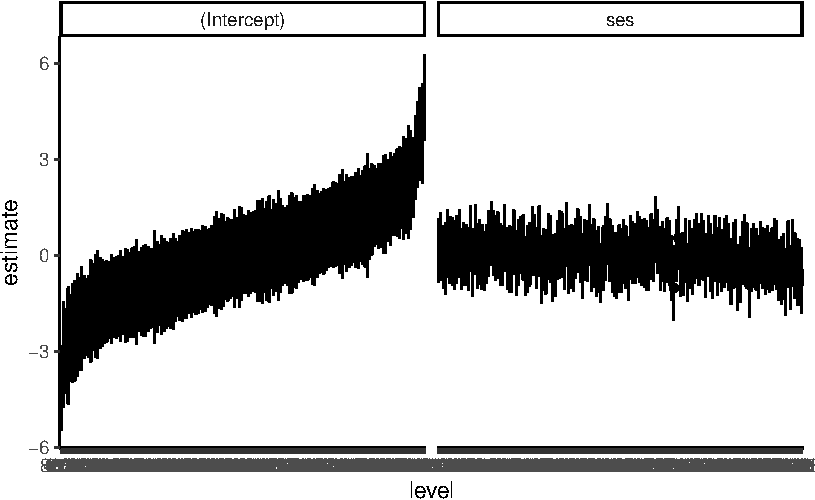
\includegraphics[width=0.7\textwidth,height=\textheight]{r_tips_files/figure-pdf/unnamed-chunk-11-1.pdf}

}

\end{figure}

\hypertarget{making-tables-in-markdown}{%
\chapter{Making tables in Markdown}\label{making-tables-in-markdown}}

You might want to make tables. You should probably make charts, but
every so often a table is a nice thing to have.

To illustrate, I make some fake data

\begin{Shaded}
\begin{Highlighting}[]
\FunctionTok{library}\NormalTok{( tidyverse )}
\NormalTok{dat }\OtherTok{=} \FunctionTok{tibble}\NormalTok{( }\AttributeTok{G =} \FunctionTok{sample}\NormalTok{( LETTERS[}\DecValTok{1}\SpecialCharTok{:}\DecValTok{5}\NormalTok{], }\DecValTok{100}\NormalTok{, }\AttributeTok{replace=}\ConstantTok{TRUE}\NormalTok{ ),}
              \AttributeTok{X =} \FunctionTok{rnorm}\NormalTok{( }\DecValTok{100}\NormalTok{ ),}
              \AttributeTok{rp =} \FunctionTok{sample}\NormalTok{( letters[}\DecValTok{1}\SpecialCharTok{:}\DecValTok{3}\NormalTok{], }\DecValTok{100}\NormalTok{, }\AttributeTok{replace=}\ConstantTok{TRUE}\NormalTok{ ),}
              \AttributeTok{Z =} \FunctionTok{sample}\NormalTok{( }\FunctionTok{c}\NormalTok{(}\StringTok{"tx"}\NormalTok{,}\StringTok{"co"}\NormalTok{), }\DecValTok{100}\NormalTok{, }\AttributeTok{replace=}\ConstantTok{TRUE}\NormalTok{ ),}
              \AttributeTok{Y =} \FunctionTok{rnorm}\NormalTok{( }\DecValTok{100}\NormalTok{ ) )}
\end{Highlighting}
\end{Shaded}

We can make summery of it by our grouping variable:

\begin{Shaded}
\begin{Highlighting}[]
\NormalTok{sdat }\OtherTok{\textless{}{-}}\NormalTok{ dat }\SpecialCharTok{\%\textgreater{}\%} \FunctionTok{group\_by}\NormalTok{( G) }\SpecialCharTok{\%\textgreater{}\%}
    \FunctionTok{summarise}\NormalTok{( }\AttributeTok{EY =} \FunctionTok{mean}\NormalTok{( Y ),}
               \AttributeTok{pT =} \FunctionTok{mean}\NormalTok{( Z }\SpecialCharTok{==} \StringTok{"tx"}\NormalTok{ ),}
               \AttributeTok{sdY =} \FunctionTok{sd}\NormalTok{( Y ) )}
\end{Highlighting}
\end{Shaded}

Our intermediate results:

\begin{Shaded}
\begin{Highlighting}[]
\NormalTok{sdat}
\end{Highlighting}
\end{Shaded}

\begin{verbatim}
# A tibble: 5 x 4
  G          EY    pT   sdY
  <chr>   <dbl> <dbl> <dbl>
1 A     -0.0390 0.25  0.715
2 B     -0.137  0.6   0.835
3 C      0.362  0.562 0.967
4 D     -0.234  0.4   0.817
5 E      0.0527 0.368 0.862
\end{verbatim}

Say our grouping variable is a set of codes for something more special.
We can merge in better names by first making a small ``cross-walk'' of
the ID codes to the full names, and then merging them to our results:

\begin{Shaded}
\begin{Highlighting}[]
\NormalTok{names }\OtherTok{=} \FunctionTok{tribble}\NormalTok{( }\SpecialCharTok{\textasciitilde{}}\NormalTok{ G, }\SpecialCharTok{\textasciitilde{}}\NormalTok{ name,}
                 \StringTok{"A"}\NormalTok{, }\StringTok{"fred"}\NormalTok{,}
                 \StringTok{"B"}\NormalTok{, }\StringTok{"doug"}\NormalTok{,}
                 \StringTok{"C"}\NormalTok{, }\StringTok{"xiao"}\NormalTok{,}
                 \StringTok{"D"}\NormalTok{, }\StringTok{"lily"}\NormalTok{,}
                 \StringTok{"E"}\NormalTok{, }\StringTok{"unknown"}\NormalTok{ )}
\NormalTok{names}
\end{Highlighting}
\end{Shaded}

\begin{verbatim}
# A tibble: 5 x 2
  G     name   
  <chr> <chr>  
1 A     fred   
2 B     doug   
3 C     xiao   
4 D     lily   
5 E     unknown
\end{verbatim}

\begin{Shaded}
\begin{Highlighting}[]
\NormalTok{sdat }\OtherTok{=} \FunctionTok{left\_join}\NormalTok{( sdat, names ) }\SpecialCharTok{\%\textgreater{}\%}
    \FunctionTok{relocate}\NormalTok{( name)}
\end{Highlighting}
\end{Shaded}

\begin{verbatim}
Joining with `by = join_by(G)`
\end{verbatim}

Finally, the easiest way to make a table is with the \texttt{kable}
command.

\begin{Shaded}
\begin{Highlighting}[]
\NormalTok{knitr}\SpecialCharTok{::}\FunctionTok{kable}\NormalTok{( sdat, }\AttributeTok{digits=}\DecValTok{2}\NormalTok{ )}
\end{Highlighting}
\end{Shaded}

\begin{longtable}[]{@{}llrrr@{}}
\toprule\noalign{}
name & G & EY & pT & sdY \\
\midrule\noalign{}
\endhead
\bottomrule\noalign{}
\endlastfoot
fred & A & -0.04 & 0.25 & 0.72 \\
doug & B & -0.14 & 0.60 & 0.83 \\
xiao & C & 0.36 & 0.56 & 0.97 \\
lily & D & -0.23 & 0.40 & 0.82 \\
unknown & E & 0.05 & 0.37 & 0.86 \\
\end{longtable}

This is a great workhorse table-making tool! There are expansion R
packages as well, e.g.~\texttt{kableExtra}, which can do lots of fancy
customizable stuff.

\hypertarget{making-a-table-one}{%
\section{Making a ``table one''}\label{making-a-table-one}}

The ``table one'' is the first table in a lot of papers that show
general means of different variables for different groups. The
\texttt{tableone} package is useful:

\begin{Shaded}
\begin{Highlighting}[]
\FunctionTok{library}\NormalTok{(tableone)}

\CommentTok{\# sample mean  }
\FunctionTok{CreateTableOne}\NormalTok{(}\AttributeTok{data =}\NormalTok{ dat,}
               \AttributeTok{vars =} \FunctionTok{c}\NormalTok{(}\StringTok{"G"}\NormalTok{, }\StringTok{"Z"}\NormalTok{, }\StringTok{"X"}\NormalTok{))}
\end{Highlighting}
\end{Shaded}

\begin{verbatim}
               
                Overall     
  n              100        
  G (%)                     
     A            20 (20.0) 
     B            20 (20.0) 
     C            16 (16.0) 
     D            25 (25.0) 
     E            19 (19.0) 
  Z = tx (%)      43 (43.0) 
  X (mean (SD)) 0.06 (1.04) 
\end{verbatim}

\begin{Shaded}
\begin{Highlighting}[]
\CommentTok{\# you can also stratify by a variables of interest}
\NormalTok{tb }\OtherTok{\textless{}{-}} \FunctionTok{CreateTableOne}\NormalTok{(}\AttributeTok{data =}\NormalTok{ dat,}
                     \AttributeTok{vars =} \FunctionTok{c}\NormalTok{(}\StringTok{"X"}\NormalTok{, }\StringTok{"G"}\NormalTok{, }\StringTok{"Y"}\NormalTok{), }
                     \AttributeTok{strata =} \FunctionTok{c}\NormalTok{(}\StringTok{"Z"}\NormalTok{))}
\NormalTok{tb}
\end{Highlighting}
\end{Shaded}

\begin{verbatim}
               Stratified by Z
                co            tx           p      test
  n                57           43                    
  X (mean (SD))  0.02 (1.13)  0.12 (0.92)   0.646     
  G (%)                                     0.163     
     A             15 (26.3)     5 (11.6)             
     B              8 (14.0)    12 (27.9)             
     C              7 (12.3)     9 (20.9)             
     D             15 (26.3)    10 (23.3)             
     E             12 (21.1)     7 (16.3)             
  Y (mean (SD)) -0.07 (0.84)  0.03 (0.85)   0.589     
\end{verbatim}

You can then use \texttt{kable} as so:

\begin{Shaded}
\begin{Highlighting}[]
\FunctionTok{print}\NormalTok{(tb}\SpecialCharTok{$}\NormalTok{ContTable, }\AttributeTok{printToggle =} \ConstantTok{FALSE}\NormalTok{) }\SpecialCharTok{\%\textgreater{}\%}
\NormalTok{    knitr}\SpecialCharTok{::}\FunctionTok{kable}\NormalTok{()}
\end{Highlighting}
\end{Shaded}

\begin{longtable}[]{@{}lllll@{}}
\toprule\noalign{}
& co & tx & p & test \\
\midrule\noalign{}
\endhead
\bottomrule\noalign{}
\endlastfoot
n & 57 & 43 & & \\
X (mean (SD)) & 0.02 (1.13) & 0.12 (0.92) & 0.646 & \\
Y (mean (SD)) & -0.07 (0.84) & 0.03 (0.85) & 0.589 & \\
\end{longtable}

\hypertarget{table-of-summary-stats}{%
\section{Table of summary stats}\label{table-of-summary-stats}}

You can also easily make pretty tables using the \texttt{stargazer}
package. You need to ensure the data is a data.frame, not tibble,
because \texttt{stargazer} is old school. It appears to only do
continuous variables.

Finally, you need to modify the R code chunk so it looks like this:

so the output of stargazer gets formatted properly in your R Markdown.

\begin{Shaded}
\begin{Highlighting}[]
\FunctionTok{library}\NormalTok{(stargazer)}

\FunctionTok{stargazer}\NormalTok{(}\FunctionTok{as.data.frame}\NormalTok{(dat))}
\end{Highlighting}
\end{Shaded}

\% Table created by stargazer v.5.2.3 by Marek Hlavac, Social Policy
Institute. E-mail: marek.hlavac at gmail.com \% Date and time: Fri, Aug
25, 2023 - 11:56:14

\begin{table}[!htbp] \centering 
  \caption{} 
  \label{} 
\begin{tabular}{@{\extracolsep{5pt}}lccccc} 
\\[-1.8ex]\hline 
\hline \\[-1.8ex] 
Statistic & \multicolumn{1}{c}{N} & \multicolumn{1}{c}{Mean} & \multicolumn{1}{c}{St. Dev.} & \multicolumn{1}{c}{Min} & \multicolumn{1}{c}{Max} \\ 
\hline \\[-1.8ex] 
X & 100 & 0.062 & 1.040 & $-$2.463 & 2.422 \\ 
Y & 100 & $-$0.026 & 0.842 & $-$1.702 & 2.154 \\ 
\hline \\[-1.8ex] 
\end{tabular} 
\end{table}

You can include only some of the variables and omit stats that are not
of interest:

\begin{Shaded}
\begin{Highlighting}[]
\CommentTok{\# to include only variables of interest}
\FunctionTok{stargazer}\NormalTok{(}\FunctionTok{as.data.frame}\NormalTok{(dat), }\AttributeTok{header=}\ConstantTok{FALSE}\NormalTok{, }
          \AttributeTok{omit.summary.stat =} \FunctionTok{c}\NormalTok{(}\StringTok{"p25"}\NormalTok{, }\StringTok{"p75"}\NormalTok{, }\StringTok{"min"}\NormalTok{, }\StringTok{"max"}\NormalTok{), }\CommentTok{\# to omit percentiles}
          \AttributeTok{title =} \StringTok{"Table 1: Descriptive statistics"}\NormalTok{)}
\end{Highlighting}
\end{Shaded}

\begin{table}[!htbp] \centering 
  \caption{Table 1: Descriptive statistics} 
  \label{} 
\begin{tabular}{@{\extracolsep{5pt}}lccc} 
\\[-1.8ex]\hline 
\hline \\[-1.8ex] 
Statistic & \multicolumn{1}{c}{N} & \multicolumn{1}{c}{Mean} & \multicolumn{1}{c}{St. Dev.} \\ 
\hline \\[-1.8ex] 
X & 100 & 0.062 & 1.040 \\ 
Y & 100 & $-$0.026 & 0.842 \\ 
\hline \\[-1.8ex] 
\end{tabular} 
\end{table}

See the \texttt{stargazer} help file for how to set/change more of the
options: https://cran.r-project.org/web/packages/stargazer/stargazer.pdf

\hypertarget{making-regression-tables-and-more-complete-summary-output}{%
\chapter{Making Regression Tables and More Complete Summary
Output}\label{making-regression-tables-and-more-complete-summary-output}}

This document demonstrates the different regression table methods, and
talks about some weird wrinkles with using them with multilevel
modeling.

\hypertarget{the-basics-of-regression-tables}{%
\section{The basics of regression
tables}\label{the-basics-of-regression-tables}}

For the basics we quickly illustrate regression tables using a subset of
the Making Caring Common dataset, which we will eventually discuss in
class. This dataset has a measure of emotional safety (our outcome) and
we want to see, in a specific school, if this is predicted by gender
and/or grade.

Our data look like this:

\begin{Shaded}
\begin{Highlighting}[]
\FunctionTok{sample\_n}\NormalTok{( sch1, }\DecValTok{6}\NormalTok{ )}
\end{Highlighting}
\end{Shaded}

\begin{verbatim}
  ID    esafe grade gender     disc race_white
1  1 3.571429     7 Female 1.111111          1
2  1 4.000000     7   Male 1.000000          0
3  1 3.714286     6 Female 3.555556          0
4  1 3.500000     6   Male 1.111111          1
5  1 4.000000     5   Male 1.000000          1
6  1 2.428571     7 Female 2.222222          1
\end{verbatim}

We fit some models:

\begin{Shaded}
\begin{Highlighting}[]
\NormalTok{M\_A }\OtherTok{=} \FunctionTok{lm}\NormalTok{( esafe }\SpecialCharTok{\textasciitilde{}}\NormalTok{ grade, }\AttributeTok{data =}\NormalTok{ sch1 )}
\NormalTok{M\_B }\OtherTok{=} \FunctionTok{lm}\NormalTok{( esafe }\SpecialCharTok{\textasciitilde{}}\NormalTok{ grade }\SpecialCharTok{+}\NormalTok{ gender, }\AttributeTok{data =}\NormalTok{ sch1 )}
\NormalTok{M\_C }\OtherTok{=} \FunctionTok{lm}\NormalTok{( esafe }\SpecialCharTok{\textasciitilde{}}\NormalTok{ grade }\SpecialCharTok{*}\NormalTok{ gender, }\AttributeTok{data =}\NormalTok{ sch1 )}
\end{Highlighting}
\end{Shaded}

Ok, we have fit our regression models. We can look at big complex
printout of a single model like so:

\begin{Shaded}
\begin{Highlighting}[]
\FunctionTok{summary}\NormalTok{( M\_C )}
\end{Highlighting}
\end{Shaded}

\begin{verbatim}

Call:
lm(formula = esafe ~ grade * gender, data = sch1)

Residuals:
    Min      1Q  Median      3Q     Max 
-1.7894 -0.1570  0.1550  0.2662  0.4938 

Coefficients:
                 Estimate Std. Error t value Pr(>|t|)    
(Intercept)       4.12733    0.37946  10.877   <2e-16 ***
grade            -0.07764    0.05859  -1.325   0.1879    
genderMale       -0.72735    0.49762  -1.462   0.1467    
grade:genderMale  0.13327    0.07627   1.747   0.0834 .  
---
Signif. codes:  0 '***' 0.001 '**' 0.01 '*' 0.05 '.' 0.1 ' ' 1

Residual standard error: 0.4333 on 108 degrees of freedom
Multiple R-squared:  0.04914,   Adjusted R-squared:  0.02273 
F-statistic: 1.861 on 3 and 108 DF,  p-value: 0.1406
\end{verbatim}

Or we can make \emph{regression tables}. There are two packages, one is
\texttt{texreg}

\begin{Shaded}
\begin{Highlighting}[]
\FunctionTok{library}\NormalTok{( texreg )}
\FunctionTok{screenreg}\NormalTok{(}\FunctionTok{list}\NormalTok{(M\_A, M\_B, M\_C))}
\end{Highlighting}
\end{Shaded}

\begin{verbatim}

====================================================
                  Model 1     Model 2     Model 3   
----------------------------------------------------
(Intercept)         3.68 ***    3.62 ***    4.13 ***
                   (0.25)      (0.25)      (0.38)   
grade               0.00        0.00       -0.08    
                   (0.04)      (0.04)      (0.06)   
genderMale                      0.13       -0.73    
                               (0.08)      (0.50)   
grade:genderMale                            0.13    
                                           (0.08)   
----------------------------------------------------
R^2                 0.00        0.02        0.05    
Adj. R^2           -0.01        0.00        0.02    
Num. obs.         112         112         112       
====================================================
*** p < 0.001; ** p < 0.01; * p < 0.05
\end{verbatim}

Another is \texttt{stargazer}.

\begin{Shaded}
\begin{Highlighting}[]
\FunctionTok{library}\NormalTok{( stargazer )}
\FunctionTok{stargazer}\NormalTok{( M\_A, M\_B, M\_C, }\AttributeTok{header=}\ConstantTok{FALSE}\NormalTok{, }\AttributeTok{type=}\StringTok{\textquotesingle{}text\textquotesingle{}}\NormalTok{)}
\end{Highlighting}
\end{Shaded}

\begin{verbatim}

===============================================================================
                                        Dependent variable:                    
                    -----------------------------------------------------------
                                               esafe                           
                            (1)                 (2)                 (3)        
-------------------------------------------------------------------------------
grade                      0.004               0.001              -0.078       
                          (0.038)             (0.038)             (0.059)      
                                                                               
genderMale                                     0.130              -0.727       
                                              (0.083)             (0.498)      
                                                                               
grade:genderMale                                                  0.133*       
                                                                  (0.076)      
                                                                               
Constant                 3.676***            3.624***            4.127***      
                          (0.249)             (0.250)             (0.379)      
                                                                               
-------------------------------------------------------------------------------
Observations                112                 112                 112        
R2                        0.0001               0.022               0.049       
Adjusted R2               -0.009               0.004               0.023       
Residual Std. Error  0.440 (df = 110)    0.437 (df = 109)    0.433 (df = 108)  
F Statistic         0.009 (df = 1; 110) 1.241 (df = 2; 109) 1.861 (df = 3; 108)
===============================================================================
Note:                                               *p<0.1; **p<0.05; ***p<0.01
\end{verbatim}

\hypertarget{extending-to-the-multilevel-model}{%
\section{Extending to the multilevel
model}\label{extending-to-the-multilevel-model}}

For our multilevel examples, we use the Making Caring Common data from
Project A, and fit data to the 8th grade students only, but do it for
all schools. We have made a High School dummy variable.

Our two models we use for demo purposes have a HS term and no HS term:

\begin{Shaded}
\begin{Highlighting}[]
\NormalTok{modA }\OtherTok{\textless{}{-}} \FunctionTok{lmer}\NormalTok{( esafe }\SpecialCharTok{\textasciitilde{}} \DecValTok{1} \SpecialCharTok{+}\NormalTok{ (}\DecValTok{1} \SpecialCharTok{|}\NormalTok{ ID), }\AttributeTok{data=}\NormalTok{dat.g8)}
\NormalTok{modB }\OtherTok{\textless{}{-}} \FunctionTok{lmer}\NormalTok{( esafe }\SpecialCharTok{\textasciitilde{}} \DecValTok{1} \SpecialCharTok{+}\NormalTok{ HS }\SpecialCharTok{+}\NormalTok{ (}\DecValTok{1} \SpecialCharTok{|}\NormalTok{ ID), }\AttributeTok{data=}\NormalTok{dat.g8)}
\end{Highlighting}
\end{Shaded}

In the next sections we first show how to get better summary output
(according to some folks) and then we walk through making regression
tables in a bit more detail than above.

\hypertarget{better-summary-output-for-lmer-getting-p-values}{%
\section{Better summary output for lmer: Getting
p-values}\label{better-summary-output-for-lmer-getting-p-values}}

The \texttt{lmerTest} package is a way of making R give you more
complete output. We are going to load it, and then put the new lmer
models into new variables so we can see how the different model fitting
packages work with the regression table packages below.

\begin{Shaded}
\begin{Highlighting}[]
\FunctionTok{library}\NormalTok{( lmerTest )}
\NormalTok{modB.T }\OtherTok{\textless{}{-}} \FunctionTok{lmer}\NormalTok{( esafe }\SpecialCharTok{\textasciitilde{}} \DecValTok{1} \SpecialCharTok{+}\NormalTok{ HS }\SpecialCharTok{+}\NormalTok{ (}\DecValTok{1} \SpecialCharTok{|}\NormalTok{ ID), }\AttributeTok{data=}\NormalTok{dat.g8)}
\NormalTok{modA.T }\OtherTok{\textless{}{-}} \FunctionTok{lmer}\NormalTok{( esafe }\SpecialCharTok{\textasciitilde{}} \DecValTok{1} \SpecialCharTok{+}\NormalTok{ (}\DecValTok{1} \SpecialCharTok{|}\NormalTok{ ID), }\AttributeTok{data=}\NormalTok{dat.g8)}

\FunctionTok{summary}\NormalTok{( modB.T )}
\end{Highlighting}
\end{Shaded}

\begin{verbatim}
Linear mixed model fit by REML. t-tests use Satterthwaite's method [
lmerModLmerTest]
Formula: esafe ~ 1 + HS + (1 | ID)
   Data: dat.g8

REML criterion at convergence: 2746.8

Scaled residuals: 
    Min      1Q  Median      3Q     Max 
-3.3883 -0.6156  0.2021  0.7628  1.7331 

Random effects:
 Groups   Name        Variance Std.Dev.
 ID       (Intercept) 0.04809  0.2193  
 Residual             0.46459  0.6816  
Number of obs: 1305, groups:  ID, 26

Fixed effects:
            Estimate Std. Error       df t value Pr(>|t|)    
(Intercept)  3.52798    0.08637 29.91033  40.846   <2e-16 ***
HSTRUE      -0.29480    0.10787 25.77814  -2.733   0.0112 *  
---
Signif. codes:  0 '***' 0.001 '**' 0.01 '*' 0.05 '.' 0.1 ' ' 1

Correlation of Fixed Effects:
       (Intr)
HSTRUE -0.801
\end{verbatim}

\hypertarget{the-texreg-package}{%
\section{The texreg package}\label{the-texreg-package}}

There are two options, one is \texttt{screenreg} and the other is
\texttt{texreg()}.

\hypertarget{screenreg}{%
\subsection{screenreg}\label{screenreg}}

Screenreg is fine for MLMs. It looks a bit like raw output, but it is
clear and clean. It will take models fit using lmer or lmerTest no
problem.

\begin{Shaded}
\begin{Highlighting}[]
\FunctionTok{screenreg}\NormalTok{(}\FunctionTok{list}\NormalTok{(modA,modB))}
\end{Highlighting}
\end{Shaded}

\begin{verbatim}

===============================================
                     Model 1       Model 2     
-----------------------------------------------
(Intercept)              3.35 ***      3.53 ***
                        (0.06)        (0.09)   
HSTRUE                                -0.29 ** 
                                      (0.11)   
-----------------------------------------------
AIC                   2756.78       2754.79    
BIC                   2772.30       2775.49    
Log Likelihood       -1375.39      -1373.40    
Num. obs.             1305          1305       
Num. groups: ID         26            26       
Var: ID (Intercept)      0.07          0.05    
Var: Residual            0.46          0.46    
===============================================
*** p < 0.001; ** p < 0.01; * p < 0.05
\end{verbatim}

\emph{Comment:} Note that the number of stars are different for the
display vs the summary output! (Look at the HS coefficient for example.)
Not good, it would seem.

This is because the \(p\)-values are calculated using the normal
approximation by the screenreg command, and using the \(t\)-test with
approximate degrees of freedom by \texttt{lmerTest}. This makes a
difference. Consider the following, using the \(t\) statistics for the
HS variable:

\begin{Shaded}
\begin{Highlighting}[]
\DecValTok{2} \SpecialCharTok{*} \FunctionTok{pt}\NormalTok{( }\SpecialCharTok{{-}}\FloatTok{2.733}\NormalTok{, }\AttributeTok{df=}\FloatTok{25.77814}\NormalTok{ )}
\end{Highlighting}
\end{Shaded}

\begin{verbatim}
[1] 0.0111831
\end{verbatim}

\begin{Shaded}
\begin{Highlighting}[]
\DecValTok{2} \SpecialCharTok{*} \FunctionTok{pnorm}\NormalTok{( }\SpecialCharTok{{-}}\FloatTok{2.733}\NormalTok{ )}
\end{Highlighting}
\end{Shaded}

\begin{verbatim}
[1] 0.006276033
\end{verbatim}

One is below 0.01, and one is not. An extra star!

\hypertarget{using-texreg-and-latex}{%
\subsection{Using texreg and latex}\label{using-texreg-and-latex}}

The \texttt{textreg} command is part of the \texttt{texreg} package and
can be integrated with latex (which you would need to install). Once you
do this, when you compile to a pdf, all is well. In the R code chunk you
need to include \texttt{results="asis"} to get the latex to compile
right. E.g., ``\texttt{r,\ results="asis"}'' when you declare a code
chunk.

\begin{Shaded}
\begin{Highlighting}[]
\FunctionTok{texreg}\NormalTok{(}\FunctionTok{list}\NormalTok{(modA,modB), }\AttributeTok{table=}\ConstantTok{FALSE}\NormalTok{)}
\end{Highlighting}
\end{Shaded}

\begin{tabular}{l c c}
\hline
 & Model 1 & Model 2 \\
\hline
(Intercept)         & $3.35^{***}$ & $3.53^{***}$ \\
                    & $(0.06)$     & $(0.09)$     \\
HSTRUE              &              & $-0.29^{**}$ \\
                    &              & $(0.11)$     \\
\hline
AIC                 & $2756.78$    & $2754.79$    \\
BIC                 & $2772.30$    & $2775.49$    \\
Log Likelihood      & $-1375.39$   & $-1373.40$   \\
Num. obs.           & $1305$       & $1305$       \\
Num. groups: ID     & $26$         & $26$         \\
Var: ID (Intercept) & $0.07$       & $0.05$       \\
Var: Residual       & $0.46$       & $0.46$       \\
\hline
\multicolumn{3}{l}{\scriptsize{$^{***}p<0.001$; $^{**}p<0.01$; $^{*}p<0.05$}}
\end{tabular}

Note that the \texttt{table=FALSE} puts the table right where you want
it, not at some random spot latex things is nice. Latex likes to have
``floating tables'' which it puts where there is space.

\hypertarget{stargazer}{%
\section{Stargazer}\label{stargazer}}

\begin{Shaded}
\begin{Highlighting}[]
\FunctionTok{library}\NormalTok{( stargazer )}
\FunctionTok{stargazer}\NormalTok{(modA, modB, }\AttributeTok{header=}\ConstantTok{FALSE}\NormalTok{, }\AttributeTok{type=}\StringTok{\textquotesingle{}latex\textquotesingle{}}\NormalTok{)}
\end{Highlighting}
\end{Shaded}

\begin{table}[!htbp] \centering 
  \caption{} 
  \label{} 
\begin{tabular}{@{\extracolsep{5pt}}lcc} 
\\[-1.8ex]\hline 
\hline \\[-1.8ex] 
 & \multicolumn{2}{c}{\textit{Dependent variable:}} \\ 
\cline{2-3} 
\\[-1.8ex] & \multicolumn{2}{c}{esafe} \\ 
\\[-1.8ex] & (1) & (2)\\ 
\hline \\[-1.8ex] 
 HS &  & $-$0.295$^{***}$ \\ 
  &  & (0.108) \\ 
  & & \\ 
 Constant & 3.346$^{***}$ & 3.528$^{***}$ \\ 
  & (0.059) & (0.086) \\ 
  & & \\ 
\hline \\[-1.8ex] 
Observations & 1,305 & 1,305 \\ 
Log Likelihood & $-$1,375.388 & $-$1,373.397 \\ 
Akaike Inf. Crit. & 2,756.775 & 2,754.795 \\ 
Bayesian Inf. Crit. & 2,772.297 & 2,775.491 \\ 
\hline 
\hline \\[-1.8ex] 
\textit{Note:}  & \multicolumn{2}{r}{$^{*}$p$<$0.1; $^{**}$p$<$0.05; $^{***}$p$<$0.01} \\ 
\end{tabular} 
\end{table}

One issue is stargazer does not include the random effect variances, so
the output is quite limited for multilevel modeling. It also has less
stringent conditions for when to put down stars. One star is below 0.10,
two is below 0.05, and three is below 0.01. This is quite generous. Also
it is using the normal approximation.

\hypertarget{stargazer-with-lmertest}{%
\subsection{Stargazer with lmerTest}\label{stargazer-with-lmertest}}

Stargazer with lmerTest is a bit fussy. This shows how to make it work
if you have loaded the lmerTest package. Recall the lmerTest package
makes your lmer commands have p-values and whatnot. But this means your
new \texttt{lmer()} command is not quite the same as the old---and
stargazer is expecting the old. You gix this by lying to R, telling it
the new thing is the old thing. This basically works.

Now for stargazer, we need to tell it that our models are the right
type. First note:

\begin{Shaded}
\begin{Highlighting}[]
\FunctionTok{class}\NormalTok{( modB )}
\end{Highlighting}
\end{Shaded}

\begin{verbatim}
[1] "lmerMod"
attr(,"package")
[1] "lme4"
\end{verbatim}

\begin{Shaded}
\begin{Highlighting}[]
\FunctionTok{class}\NormalTok{( modB.T)}
\end{Highlighting}
\end{Shaded}

\begin{verbatim}
[1] "lmerModLmerTest"
attr(,"package")
[1] "lmerTest"
\end{verbatim}

So we fix as follows:

\begin{Shaded}
\begin{Highlighting}[]
\FunctionTok{library}\NormalTok{( stargazer )}
\FunctionTok{class}\NormalTok{( modB.T ) }\OtherTok{=} \StringTok{"lmerMod"} 
\FunctionTok{class}\NormalTok{( modA.T ) }\OtherTok{=} \StringTok{"lmerMod"} 
\FunctionTok{stargazer}\NormalTok{(modA.T, modB.T, }\AttributeTok{header=}\ConstantTok{FALSE}\NormalTok{, }\AttributeTok{type=}\StringTok{\textquotesingle{}latex\textquotesingle{}}\NormalTok{ )}
\end{Highlighting}
\end{Shaded}

\begin{table}[!htbp] \centering 
  \caption{} 
  \label{} 
\begin{tabular}{@{\extracolsep{5pt}}lcc} 
\\[-1.8ex]\hline 
\hline \\[-1.8ex] 
 & \multicolumn{2}{c}{\textit{Dependent variable:}} \\ 
\cline{2-3} 
\\[-1.8ex] & \multicolumn{2}{c}{esafe} \\ 
\\[-1.8ex] & (1) & (2)\\ 
\hline \\[-1.8ex] 
 HS &  & $-$0.295$^{***}$ \\ 
  &  & (0.108) \\ 
  & & \\ 
 Constant & 3.346$^{***}$ & 3.528$^{***}$ \\ 
  & (0.059) & (0.086) \\ 
  & & \\ 
\hline \\[-1.8ex] 
Observations & 1,305 & 1,305 \\ 
Log Likelihood & $-$1,375.388 & $-$1,373.397 \\ 
Akaike Inf. Crit. & 2,756.775 & 2,754.795 \\ 
Bayesian Inf. Crit. & 2,772.297 & 2,775.491 \\ 
\hline 
\hline \\[-1.8ex] 
\textit{Note:}  & \multicolumn{2}{r}{$^{*}$p$<$0.1; $^{**}$p$<$0.05; $^{***}$p$<$0.01} \\ 
\end{tabular} 
\end{table}

\hypertarget{pretty-anova-tables-with-kable}{%
\chapter{\texorpdfstring{Pretty ANOVA Tables with
\texttt{kable}}{Pretty ANOVA Tables with kable}}\label{pretty-anova-tables-with-kable}}

\hypertarget{r-setup}{%
\section{R Setup}\label{r-setup}}

We load the \texttt{tidyverse} and \texttt{knitr}. The \texttt{kable}
function from \texttt{knitr} makes our tables look nice!

\begin{Shaded}
\begin{Highlighting}[]
\FunctionTok{library}\NormalTok{(tidyverse)}
\FunctionTok{library}\NormalTok{(knitr)}
\FunctionTok{library}\NormalTok{(broom)}
\end{Highlighting}
\end{Shaded}

\hypertarget{create-fake-data}{%
\section{Create fake data}\label{create-fake-data}}

We create a data set called \texttt{a} that has 100 observations and
specifies our outcome \texttt{Y} as a funciton of two uncorrelated
variables \texttt{A} and \texttt{B}

\begin{Shaded}
\begin{Highlighting}[]
\NormalTok{a }\OtherTok{\textless{}{-}} \FunctionTok{tibble}\NormalTok{( }\AttributeTok{A =} \FunctionTok{rnorm}\NormalTok{( }\DecValTok{100}\NormalTok{ ),}
            \AttributeTok{B =} \FunctionTok{rnorm}\NormalTok{( }\DecValTok{100}\NormalTok{ ),}
            \AttributeTok{Y =}\NormalTok{ A }\SpecialCharTok{*} \FloatTok{0.2} \SpecialCharTok{+}\NormalTok{ B }\SpecialCharTok{*} \FloatTok{0.5} \SpecialCharTok{+} \FunctionTok{rnorm}\NormalTok{( }\DecValTok{100}\NormalTok{, }\DecValTok{0}\NormalTok{, }\DecValTok{1}\NormalTok{ ) )}
\end{Highlighting}
\end{Shaded}

\hypertarget{run-the-models}{%
\section{Run the Models}\label{run-the-models}}

We fit two models, one with \texttt{A} and \texttt{B}, the other with
just \texttt{A}.

\begin{Shaded}
\begin{Highlighting}[]
\NormalTok{M1 }\OtherTok{\textless{}{-}} \FunctionTok{lm}\NormalTok{( Y}\SpecialCharTok{\textasciitilde{}}\NormalTok{ A }\SpecialCharTok{+}\NormalTok{ B, }\AttributeTok{data =}\NormalTok{ a )}
\NormalTok{M2 }\OtherTok{\textless{}{-}} \FunctionTok{lm}\NormalTok{( Y }\SpecialCharTok{\textasciitilde{}}\NormalTok{ A, }\AttributeTok{data =}\NormalTok{ a )}
\end{Highlighting}
\end{Shaded}

\hypertarget{comparing-the-models}{%
\section{Comparing the Models}\label{comparing-the-models}}

We use the \texttt{anova} function to compare the two models (see also
the chapter on Likelihood Ratio tests). We see that \texttt{B} improves
the model fit significantly.

\begin{Shaded}
\begin{Highlighting}[]
\NormalTok{aa }\OtherTok{=} \FunctionTok{anova}\NormalTok{( M2, M1 )}
\NormalTok{aa}
\end{Highlighting}
\end{Shaded}

\begin{verbatim}
Analysis of Variance Table

Model 1: Y ~ A
Model 2: Y ~ A + B
  Res.Df    RSS Df Sum of Sq      F    Pr(>F)    
1     98 133.28                                  
2     97 109.26  1    24.018 21.322 1.192e-05 ***
---
Signif. codes:  0 '***' 0.001 '**' 0.01 '*' 0.05 '.' 0.1 ' ' 1
\end{verbatim}

\begin{Shaded}
\begin{Highlighting}[]
\NormalTok{aa }\SpecialCharTok{|\textgreater{}} 
  \FunctionTok{tidy}\NormalTok{() }\SpecialCharTok{|\textgreater{}} 
  \FunctionTok{kable}\NormalTok{()}
\end{Highlighting}
\end{Shaded}

\begin{longtable}[]{@{}lrrrrrr@{}}
\toprule\noalign{}
term & df.residual & rss & df & sumsq & statistic & p.value \\
\midrule\noalign{}
\endhead
\bottomrule\noalign{}
\endlastfoot
Y \textasciitilde{} A & 98 & 133.2799 & NA & NA & NA & NA \\
Y \textasciitilde{} A + B & 97 & 109.2623 & 1 & 24.01766 & 21.32221 &
1.19e-05 \\
\end{longtable}

\hypertarget{compare-to-the-significance-test-on-b}{%
\section{\texorpdfstring{Compare to the Significance test on
\texttt{B}}{Compare to the Significance test on B}}\label{compare-to-the-significance-test-on-b}}

Note that the p value for \texttt{B} is identical to the ANOVA results
above. Why bother with ANOVA? It can test more complex hypotheses as
well (multiple coefficients, random effects, etc.)

\begin{Shaded}
\begin{Highlighting}[]
\NormalTok{M1 }\SpecialCharTok{|\textgreater{}} 
  \FunctionTok{tidy}\NormalTok{() }\SpecialCharTok{|\textgreater{}} 
  \FunctionTok{kable}\NormalTok{()}
\end{Highlighting}
\end{Shaded}

\begin{longtable}[]{@{}lrrrr@{}}
\toprule\noalign{}
term & estimate & std.error & statistic & p.value \\
\midrule\noalign{}
\endhead
\bottomrule\noalign{}
\endlastfoot
(Intercept) & -0.0391383 & 0.1069672 & -0.365891 & 0.7152432 \\
A & 0.1949385 & 0.1091445 & 1.786058 & 0.0772145 \\
B & 0.5391913 & 0.1167688 & 4.617598 & 0.0000119 \\
\end{longtable}

\hypertarget{a-math-reference-sample-modeling-equations-to-borrow}{%
\chapter{A Math Reference: Sample Modeling Equations to
Borrow}\label{a-math-reference-sample-modeling-equations-to-borrow}}

\hypertarget{introduction}{%
\section{Introduction}\label{introduction}}

This document has a bunch of mathematical equations we use in the class.
It is a good reference for how to write your own math equations in your
life moving forward. Generally, people write math equations using
something called Latex. Latex (or Tex) is a way of writing documents
where mixed in with the writing of what you want to say are commands
describing how you want your document to look. This is a very powerful
thing: there are Tex editors that allow you to write entire articles,
books, reports, poetry, or whatever with extreme control over the
typesetting used. It creates beautifully typeset documents that are easy
to distinguish from those written in, say, MS Word due to how they
adjust whitespace on the page. That being said, it can be a lot to jump
in to.

Enter R Markdown. R Markdown is a useful and easy way to take advantage
of this syntax without the overhead of writing entire documents in
Latex, even if you don't have any R code in your document. Inside R
Markdown you can write math equations, and then when you render the
report, it not only runs all the R code, but it formats all the math for
you as well! You can even have R Markdown render to MS Word to give you
a word doc with all your math equations ready to go.

\hypertarget{using-this-document}{%
\subsection{Using this document}\label{using-this-document}}

You are probably reading the PDF version of this document. But really
you should open the .Rmd file and cut and paste the relevant equations
into your own work, and then modify as necessary.

\hypertarget{overview-of-using-latex}{%
\section{Overview of Using Latex}\label{overview-of-using-latex}}

For math in your writing, you denote the beginning and the end of a math
equation in your text using ``\$''s---one at the start and one at the
stop. E.g., ``\$ math stuff \$''. Most greek letters are written as
their names with a backslash ``\textbackslash{}'' just before it. E.g.,
``\textbackslash alpha''.

So if I want to write an alpha, I write ``\$\textbackslash alpha\$'' and
get \(\alpha\).

I can do subscripts by using an underscore. E.g.,
``\$\textbackslash alpha\_j\$'' gives \(\alpha_j\). I can also do
superscripts by using a hat. E.g., ``\$\textbackslash alpha\^{}2\$''
gives \(\alpha^2\).

\newpage

\hypertarget{some-useful-greek-letters}{%
\subsection{Some useful greek letters}\label{some-useful-greek-letters}}

Here are some useful greek letters and symbols

\begin{longtable}[]{@{}rr@{}}
\toprule\noalign{}
Letter & Name \\
\midrule\noalign{}
\endhead
\bottomrule\noalign{}
\endlastfoot
\(\alpha\) & \textbackslash alpha \\
\(\beta\) & \textbackslash beta \\
\(\delta, \Delta\) & \textbackslash delta, \textbackslash Delta \\
\(\epsilon\) & \textbackslash epsilon \\
\(\sigma, \Sigma\) & \textbackslash sigma, \textbackslash Sigma \\
\(\rho\) & \textbackslash rho \\
\(\mu\) & \textbackslash mu (Meew!) \\
\(\tau\) & \textbackslash tau \\
\(\times\) & \textbackslash times \\
\(\sim\) & \textbackslash sim \\
\end{longtable}

See many more symbols at, e.g.,
\url{https://www.caam.rice.edu/~heinken/latex/symbols.pdf}. This was
found by searching ``tex symbols'' on Google.

\hypertarget{equations-on-lines-by-themselves}{%
\subsection{Equations on lines by
themselves}\label{equations-on-lines-by-themselves}}

To write an equation on a line by itself, put the math stuff in between
a pair of double ``\$''. E.g., if we write:

\begin{verbatim}
$$ Y = a X + b $$
\end{verbatim}

We get \[ Y = a X + b \]

If we want multiple lines, we have to put our equation between a
\texttt{\textbackslash{}begin\{aligned\}} and
\texttt{\textbackslash{}end\{aligned\}} command and use a double
backslash (``\textbackslash\textbackslash{}'') to denote each line break
(even if we have a line break we have to do this---we have to explicitly
tell the program converting our raw text to nice formatted text where
the line breaks are). Finally, inside the begin-end block of math, line
things up with \texttt{\&} symbols on each row of our equation. The
\texttt{\&} symbols will be lined up vertically.

So if we write

\begin{verbatim}
$$
\begin{aligned}
Y &= 10 X + 2 \\
Y - 5 &= 3 X^2 + 5
\end{aligned}
$$
\end{verbatim}

we get \[
\begin{aligned}
Y &= 10 X + 2 \\
Y - 5 &= 3 X^2 + 5
\end{aligned}
\] Also consider:

\begin{verbatim}
$$
\begin{aligned}
a + b + c + d &= c \\
 d &= e + f + g + h 
\end{aligned}
$$
\end{verbatim}

giving \[
\begin{aligned}
a + b + c + d &= c \\
 d &= e + f + g + h 
\end{aligned}
\]

\hypertarget{normal-text-in-equations}{%
\subsection{Normal text in equations}\label{normal-text-in-equations}}

If you put words in your equations, they get all italliced and weird,
without their spaces:

\begin{verbatim}
$$
5 + my dog = 10
$$
\end{verbatim}

\[
5 + my dog = 10
\]

You can fix using the ``\textbackslash mbox\{\}'' command as so:

\begin{verbatim}
$$
5 + \mbox{my dog} = 10
$$
\end{verbatim}

\[
5 + \mbox{my dog} = 10
\]

We next walk through some latex code for the models you will most see.

\hypertarget{random-intercept-model}{%
\section{Random Intercept Model}\label{random-intercept-model}}

Our canonical Random Intercept model is as follows. First, our Level 1
model:

\begin{verbatim}
$$
\begin{aligned}
y_{ij} &= \alpha_{j} + \beta_{1} ses_{ij} +  \epsilon_{ij} \\
\epsilon_{ij} &\sim N( 0, \sigma^2_y ) \\
\end{aligned}
$$
\end{verbatim}

\[
\begin{aligned}
y_{ij} &= \alpha_{j} + \beta_{1} ses_{ij} +  \epsilon_{ij} \\
\epsilon_{ij} &\sim N( 0, \sigma^2_y ) \\
\end{aligned}
\]

Our Level 2 model:

\begin{verbatim}
$$
\begin{aligned}
\alpha_{j} &= \gamma_{0} + \gamma_{1} sector_j + u_{j} \\
u_{j} &\sim N( 0, \sigma^2_\alpha ) \\
\end{aligned}
$$
\end{verbatim}

\[
\begin{aligned}
\alpha_{j} &= \gamma_{0} + \gamma_{1} sector_j + u_{j} \\
u_{j} &\sim N( 0, \sigma^2_\alpha ) \\
\end{aligned}
\]

The Gelman and Hill bracket notation looks like this:

\begin{verbatim}
$$
\begin{aligned}
y_{i} &= \alpha_{j[i]} + \beta_{1} ses_{i} +  \epsilon_{i} \\
\epsilon_i &\sim N( 0, \sigma^2_y ) \\
\alpha_{j} &= \gamma_{0} + \gamma_{1} sector_j + u_{j} \\
u_{j} &\sim N( 0, \sigma^2_\alpha ) \\
\end{aligned}
$$
\end{verbatim}

\[
\begin{aligned}
y_{i} &= \alpha_{j[i]} + \beta_{1} ses_{i} +  \epsilon_{i} \\
\epsilon_i &\sim N( 0, \sigma^2_y ) \\
\alpha_{j} &= \gamma_{0} + \gamma_{1} sector_j + u_{j} \\
u_{j} &\sim N( 0, \sigma^2_\alpha ) \\
\end{aligned}
\]

The reduced form would look like this:

\begin{verbatim}
$$
y_{i} = \gamma_{0} + \gamma_{1} sector_{j[i]} + \beta_{1} ses_{i} + u_{j[i]} + \epsilon_{i}
$$
\end{verbatim}

\[
y_{i} = \gamma_{0} + \gamma_{1} sector_{j[i]} + \beta_{1} ses_{i} + u_{j[i]} + \epsilon_{i}
\]

with

\begin{verbatim}
$$
\epsilon_i \sim N( 0, \sigma^2_y ), \mbox{ and } u_{j} \sim N( 0, \sigma^2_\alpha )
$$
\end{verbatim}

\[
\epsilon_i \sim N( 0, \sigma^2_y ), \mbox{ and } u_{j} \sim N( 0, \sigma^2_\alpha )
\]

If we want to be really prissy, we can write down the i.i.d. aspect of
our random effects like this

\begin{verbatim}
$$
\epsilon_i \stackrel{i.i.d}{\sim} N( 0, \sigma^2_y ), 
\mbox{ and } u_{j} \stackrel{i.i.d}{\sim} N( 0, \sigma^2_\alpha )
$$
\end{verbatim}

\[
\epsilon_i \stackrel{i.i.d}{\sim} N( 0, \sigma^2_y ), \\
\mbox{ and } u_{j} \stackrel{i.i.d}{\sim} N( 0, \sigma^2_\alpha )
\] The \texttt{\textbackslash{}stackrel\{\}\{\}} command takes two bits
of latex, each in the curly braces, and stacks them on top of each
other.

\hypertarget{random-slope-model}{%
\section{Random Slope Model}\label{random-slope-model}}

The canonical random slope model for HS\&B with \texttt{ses} at level 1
and sector at level 2

Level 1 models:

\begin{verbatim}
$$
\begin{aligned}
y_{ij} &= \beta_{0j} + \beta_{1j} ses_{ij} +  \epsilon_{ij} \\
\epsilon_{ij} &\sim N( 0, \sigma^2_y ) \\
\end{aligned}
$$
\end{verbatim}

\[
\begin{aligned}
y_{ij} &= \beta_{0j} + \beta_{1j} ses_{ij} +  \epsilon_{ij} \\
\epsilon_{ij} &\sim N( 0, \sigma^2_y ) \\
\end{aligned}
\]

Level 2 models:

\begin{verbatim}
$$
\begin{aligned}
\beta_{0j} &= \gamma_{00} + \gamma_{01} sector_j + u_{0j} \\
\beta_{1j} &= \gamma_{10} + \gamma_{11} sector_j + u_{1j} 
\end{aligned}
$$
\end{verbatim}

\[
\begin{aligned}
\beta_{0j} &= \gamma_{00} + \gamma_{01} sector_j + u_{0j} \\
\beta_{1j} &= \gamma_{10} + \gamma_{11} sector_j + u_{1j} 
\end{aligned}
\]

with

\begin{verbatim}
$$
\begin{pmatrix} u_{0j} \\
u_{1j}
\end{pmatrix} \sim  N
\begin{bmatrix}
\begin{pmatrix}
0 \\
0
\end{pmatrix}\!\!,&
\begin{pmatrix}
\tau_{00} & \tau_{01}\\
 & \tau_{11} \\
\end{pmatrix}
\end{bmatrix}
$$
\end{verbatim}

\[
\begin{pmatrix} u_{0j} \\
u_{1j}
\end{pmatrix} \sim  N
\begin{bmatrix}
\begin{pmatrix}
0 \\
0
\end{pmatrix}\!\!,&
\begin{pmatrix}
\tau_{00} & \tau_{01}\\
 & \tau_{11} \\
\end{pmatrix}
\end{bmatrix}
\]

The derivation of the reduced form is:

\begin{verbatim}
$$
\begin{aligned}
y_{ij} &= \beta_{0j} + \beta_{1j} ses_{ij} + \epsilon_{ij}\\
&= \left( \gamma_{00} + \gamma_{01} sector_j + u_{0j} \right)+ \\\
  (\gamma_{10} + \gamma_{11} sector_j + u_{1j}) ses_{ij} +  \epsilon_{ij} \\
&= \gamma_{00} + \gamma_{01} sector_j + u_{0j}  + \gamma_{10}ses_{ij} + \\
  \gamma_{11} sector_j ses_{ij} + u_{1j} ses_{ij} +  \epsilon_{ij}  \\
&= \gamma_{00} + \gamma_{01} sector_j +  \gamma_{10}ses_{ij} + \\
  \gamma_{11} sector_j ses_{ij} + \left(u_{0j} + u_{1j} ses_{ij} + \epsilon_{ij} \right) 
\end{aligned}
$$
\end{verbatim}

\[
\begin{aligned}
y_{ij} &= \beta_{0j} + \beta_{1j} ses_{ij} + \epsilon_{ij}\\
&= \left( \gamma_{00} + \gamma_{01} sector_j + u_{0j} \right)+ (\gamma_{10} + \gamma_{11} sector_j + u_{1j}) ses_{ij} +  \epsilon_{ij} \\
&= \gamma_{00} + \gamma_{01} sector_j + u_{0j}  + \gamma_{10}ses_{ij} + \gamma_{11} sector_j ses_{ij} + u_{1j} ses_{ij} +  \epsilon_{ij}  \\
&= \gamma_{00} + \gamma_{01} sector_j +  \gamma_{10}ses_{ij} + \gamma_{11} sector_j ses_{ij} + \left(u_{0j} + u_{1j} ses_{ij} + \epsilon_{ij} \right) 
\end{aligned}
\]

\emph{Commentary:} There are various and competing ways of writing the
covariance matrix for the random effects. The \(\tau_{**}\) notation is
easy and expands to any sized matrix (if we, for example, have more than
one random slope). But all the \(\tau_{**}\) are variances, not standard
deviations, and we often like to talk about random effect variation in
terms of standard deviations. We can thus use something like this
instead:

\begin{verbatim}
$$
\begin{pmatrix} u_{0j} \\
u_{1j}
\end{pmatrix} \sim  N
\begin{bmatrix}
\begin{pmatrix}
0 \\
0
\end{pmatrix}\!\!,&
\begin{pmatrix}
\sigma^2_{0} & \rho \sigma_0 \sigma_1 \\
 & \sigma^2_{1} \\
\end{pmatrix}
\end{bmatrix}
$$
\end{verbatim}

\[
\begin{pmatrix} u_{0j} \\
u_{1j}
\end{pmatrix} \sim  N
\begin{bmatrix}
\begin{pmatrix}
0 \\
0
\end{pmatrix}\!\!,&
\begin{pmatrix}
\sigma^2_{0} & \rho \sigma_0 \sigma_1 \\
 & \sigma^2_{1} \\
\end{pmatrix}
\end{bmatrix}
\]

Here we have a correlation of random effects, \(\rho\), instead of a
covariance, \(\tau_{01}\). And we can talk about the standard deviation
of, e.g., the random intercepts, as \(\sigma_0\) rather than
\(\sqrt{ \tau_{00} }\). Different ways of writing the same mathematical
thing are called different \emph{parameterizations}; they are
equivalent, but are more or less clear for different contexts.\\
Unfortunately, this means there is no one right answer for how to write
down a mathematical equation!

\hypertarget{summations-and-fancy-stuff}{%
\section{Summations and fancy stuff}\label{summations-and-fancy-stuff}}

Fractions are as follows:

\begin{verbatim}
$$
cor( A, B ) = \frac{ cov( A, B ) }{ \sigma_A \sigma_B }
$$
\end{verbatim}

\[
cor( A, B ) = \frac{ cov( A, B ) }{ \sigma_A \sigma_B }
\]

For reference, you can do summations and whatnot as follows:

\begin{verbatim}
$$
Var( Y_{i} ) = \frac{1}{n-1} \sum_{i=1}^n \left( Y_{i} - \bar{Y} \right)^2 
$$
\end{verbatim}

\[
Var( Y_{i} ) = \frac{1}{n-1} \sum_{i=1}^n \left( Y_{i} - \bar{Y} \right)^2 
\]

And if you have fractions you can have big brackets with
``\textbackslash left('' and ``\textbackslash right)'' as follows:

\begin{verbatim}
$$
X = \left( \frac{1}{2} + y \right)
$$
\end{verbatim}

\[
X = \left( \frac{1}{2} + y \right)
\]

Annoyingly, you always need a pair of these big brackets. If you really
don't want one, you use a backslash and a dot, like so:

\begin{verbatim}
$$
X = \left( \frac{1}{2} + y \right.
$$
\end{verbatim}

\[
X = \left( \frac{1}{2} + y \right.
\]

The rest you can find on StackOverflow or similar. Or perhaps have
ChatGPT help you write your code!

\hypertarget{pivot_longer-and-pivot_wider}{%
\chapter{\texorpdfstring{\texttt{pivot\_longer} and
\texttt{pivot\_wider}}{pivot\_longer and pivot\_wider}}\label{pivot_longer-and-pivot_wider}}

Generally, you want your data to be in a form where each row is a case
and each column is a variable (either explanatory or response).
Sometimes your data don't start that way. This section describes how to
move your data around to get it in that form. The tidyverse provides a
simple method for doing this (\texttt{pivot\_longer()} and
\texttt{pivot\_wider()}) which you should read about in R for Data
Science. There are also ``old school'' ways of doing this, via a method
called \texttt{reshape()}; this way is more powerful and useful in some
circumstances. See the final section for more on this old-style
approach.

But for now, the pivot methods will pretty much do everything you want.
Both \texttt{pivot\_longer} and \texttt{pivot\_wider} from
\texttt{tidyverse} are great functions to understand. First, we load
\texttt{tidyverse} and make some fake data.

\begin{Shaded}
\begin{Highlighting}[]
\FunctionTok{library}\NormalTok{(tidyverse)}

\NormalTok{dat }\OtherTok{\textless{}{-}} \FunctionTok{data.frame}\NormalTok{( }\AttributeTok{ID =} \FunctionTok{c}\NormalTok{( }\DecValTok{1}\SpecialCharTok{:}\DecValTok{3}\NormalTok{ ), }
                  \AttributeTok{X =} \FunctionTok{c}\NormalTok{( }\DecValTok{10}\NormalTok{, }\DecValTok{20}\NormalTok{, }\DecValTok{30}\NormalTok{ ),}
                  \AttributeTok{Y1 =} \DecValTok{1}\SpecialCharTok{:}\DecValTok{3}\NormalTok{,}
                  \AttributeTok{Y2 =} \DecValTok{10} \SpecialCharTok{+} \DecValTok{1}\SpecialCharTok{:}\DecValTok{3}\NormalTok{,}
                  \AttributeTok{Y3 =} \DecValTok{20} \SpecialCharTok{+} \DecValTok{1}\SpecialCharTok{:}\DecValTok{3}\NormalTok{ )}

\NormalTok{dat}
\end{Highlighting}
\end{Shaded}

\begin{verbatim}
  ID  X Y1 Y2 Y3
1  1 10  1 11 21
2  2 20  2 12 22
3  3 30  3 13 23
\end{verbatim}

This data is in wide format, where we have multiple measurements (Y1,
Y2, and Y3) for each individual (each row of data). We use
\texttt{pivot\_longer} to take our \texttt{Y} values and nest them
within each \texttt{ID} for longitudinal MLM analysis. (NB you can use
SEM to fit longitudinal models with wide data; we do not explore that
application here.)

\begin{Shaded}
\begin{Highlighting}[]
\NormalTok{datL }\OtherTok{\textless{}{-}} \FunctionTok{pivot\_longer}\NormalTok{(dat, Y1}\SpecialCharTok{:}\NormalTok{Y3, }
                     \AttributeTok{names\_to =} \StringTok{"time"}\NormalTok{, }
                     \AttributeTok{values\_to =} \StringTok{"front"}\NormalTok{ )}

\NormalTok{datL}
\end{Highlighting}
\end{Shaded}

\begin{verbatim}
# A tibble: 9 x 4
     ID     X time  front
  <int> <dbl> <chr> <dbl>
1     1    10 Y1        1
2     1    10 Y2       11
3     1    10 Y3       21
4     2    20 Y1        2
5     2    20 Y2       12
6     2    20 Y3       22
7     3    30 Y1        3
8     3    30 Y2       13
9     3    30 Y3       23
\end{verbatim}

\texttt{pivot\_wider} takes us back in the other direction.

\begin{Shaded}
\begin{Highlighting}[]
\NormalTok{newdat }\OtherTok{\textless{}{-}} \FunctionTok{pivot\_wider}\NormalTok{( datL, }\FunctionTok{c}\NormalTok{(ID, X), }
                       \AttributeTok{names\_from=}\NormalTok{time, }
                       \AttributeTok{values\_from=}\NormalTok{front  )}

\NormalTok{newdat}
\end{Highlighting}
\end{Shaded}

\begin{verbatim}
# A tibble: 3 x 5
     ID     X    Y1    Y2    Y3
  <int> <dbl> <dbl> <dbl> <dbl>
1     1    10     1    11    21
2     2    20     2    12    22
3     3    30     3    13    23
\end{verbatim}

We then verify our work with a few checks.

\begin{Shaded}
\begin{Highlighting}[]
\FunctionTok{stopifnot}\NormalTok{( }\FunctionTok{length}\NormalTok{( }\FunctionTok{unique}\NormalTok{( newdat}\SpecialCharTok{$}\NormalTok{ID ) ) }\SpecialCharTok{==} \FunctionTok{nrow}\NormalTok{( newdat ) )}

\NormalTok{students }\OtherTok{=}\NormalTok{ datL }\SpecialCharTok{\%\textgreater{}\%}\NormalTok{ dplyr}\SpecialCharTok{::}\FunctionTok{select}\NormalTok{( ID, X ) }\SpecialCharTok{\%\textgreater{}\%}
    \FunctionTok{unique}\NormalTok{()}
\NormalTok{students}
\end{Highlighting}
\end{Shaded}

\begin{verbatim}
# A tibble: 3 x 2
     ID     X
  <int> <dbl>
1     1    10
2     2    20
3     3    30
\end{verbatim}

\begin{Shaded}
\begin{Highlighting}[]
\NormalTok{students }\OtherTok{=} \FunctionTok{merge}\NormalTok{( students, newdat, }\AttributeTok{by=}\StringTok{"ID"}\NormalTok{ )}
\end{Highlighting}
\end{Shaded}

\hypertarget{optional-using-old-school-reshape}{%
\section{\texorpdfstring{Optional: Using old School
\texttt{reshape}}{Optional: Using old School reshape}}\label{optional-using-old-school-reshape}}

Say you have data in a form where a row has a value for a variable for
several different points in time. The following code turns it into a
data.frame where each row (case) is a value for the variable at that
point in time. You also have an ID variable for which Country the GDP
came from.

\begin{Shaded}
\begin{Highlighting}[]
\NormalTok{dtw }\OtherTok{=} \FunctionTok{read.csv}\NormalTok{( }\StringTok{"data/fake\_country\_block.csv"}\NormalTok{, }\AttributeTok{as.is=}\ConstantTok{TRUE}\NormalTok{ )}
\NormalTok{dtw}
\end{Highlighting}
\end{Shaded}

\begin{verbatim}
  Country X1997 X1998 X1999 X2000 X2001 X2002 X2003 X2004
1   China   0.5     1     2   3.4     4   5.3   6.0     7
2 Morocco  31.9    32    33  34.0    NA  36.0  37.0    NA
3 England  51.3    52    53  54.3    55  56.0  57.3    58
\end{verbatim}

Here we have three rows, but actually a lot of cases if we consider each
time point a case. For trying it on your own, get the sample csv file
(){[}here{]}\\
See the website to get the sample csv file
\textbackslash verb\textbar fake\_country\_block.csv\textbar.

The following \emph{reshapes} our original data by making a case for
each time point:

\begin{Shaded}
\begin{Highlighting}[]
\NormalTok{dt }\OtherTok{=} \FunctionTok{reshape}\NormalTok{( dtw, }\AttributeTok{idvar=}\StringTok{"Country"}\NormalTok{, }\AttributeTok{timevar=}\StringTok{"Year"}\NormalTok{, }\AttributeTok{varying=}\DecValTok{2}\SpecialCharTok{:}\DecValTok{9}\NormalTok{, }\AttributeTok{sep=}\StringTok{""}\NormalTok{, }\AttributeTok{direction=}\StringTok{"long"}\NormalTok{ )}
\FunctionTok{head}\NormalTok{(dt)}
\end{Highlighting}
\end{Shaded}

\begin{verbatim}
             Country Year    X
China.1997     China 1997  0.5
Morocco.1997 Morocco 1997 31.9
England.1997 England 1997 51.3
China.1998     China 1998  1.0
Morocco.1998 Morocco 1998 32.0
England.1998 England 1998 52.0
\end{verbatim}

Things to notice: each case has a ``row name'' made out of the country
and the Year. The ``2:9'' indicates a range of columns for the variable
that is actually the same variable.\\
R picked up that, for each of these columns, ``X'' is the name of the
variable and the number is the time, and seperated them. You can set the
name of your time variable, \textbackslash verb\textbar timevar\textbar,
to whatever you want.

The above output is called ``long format'' and the prior is called
``wide format.''\\
You can go in either direction. Here:

\begin{Shaded}
\begin{Highlighting}[]
\NormalTok{dtn }\OtherTok{=} \FunctionTok{reshape}\NormalTok{( dt, }\AttributeTok{idvar=}\StringTok{"Country"}\NormalTok{, }\AttributeTok{timevar=}\StringTok{"Year"}\NormalTok{ )}
\NormalTok{dtn}
\end{Highlighting}
\end{Shaded}

\begin{verbatim}
             Country X.1997 X.1998 X.1999 X.2000 X.2001 X.2002 X.2003 X.2004
China.1997     China    0.5      1      2    3.4      4    5.3    6.0      7
Morocco.1997 Morocco   31.9     32     33   34.0     NA   36.0   37.0     NA
England.1997 England   51.3     52     53   54.3     55   56.0   57.3     58
\end{verbatim}

You can reshape on multiple variables. For example:

\begin{Shaded}
\begin{Highlighting}[]
\NormalTok{exp.dat }\OtherTok{=} \FunctionTok{data.frame}\NormalTok{( }\AttributeTok{ID=}\FunctionTok{c}\NormalTok{(}\StringTok{"a"}\NormalTok{,}\StringTok{"b"}\NormalTok{,}\StringTok{"c"}\NormalTok{,}\StringTok{"d"}\NormalTok{), }
      \AttributeTok{cond =} \FunctionTok{c}\NormalTok{(}\StringTok{"AI"}\NormalTok{,}\StringTok{"DI"}\NormalTok{,}\StringTok{"DI"}\NormalTok{,}\StringTok{"AI"}\NormalTok{),}
            \AttributeTok{trial1 =} \FunctionTok{c}\NormalTok{(}\StringTok{"E"}\NormalTok{,}\StringTok{"U"}\NormalTok{,}\StringTok{"U"}\NormalTok{,}\StringTok{"E"}\NormalTok{),}
            \AttributeTok{dec1 =} \FunctionTok{c}\NormalTok{(}\DecValTok{1}\NormalTok{,}\DecValTok{1}\NormalTok{,}\DecValTok{0}\NormalTok{,}\DecValTok{1}\NormalTok{),}
            \AttributeTok{trial2 =} \FunctionTok{c}\NormalTok{(}\StringTok{"U"}\NormalTok{,}\StringTok{"E"}\NormalTok{,}\StringTok{"U"}\NormalTok{,}\StringTok{"E"}\NormalTok{),}
            \AttributeTok{dec2 =} \FunctionTok{c}\NormalTok{(}\DecValTok{0}\NormalTok{,}\DecValTok{0}\NormalTok{,}\DecValTok{0}\NormalTok{,}\DecValTok{1}\NormalTok{),}
                \AttributeTok{trial3 =} \FunctionTok{c}\NormalTok{(}\StringTok{"U"}\NormalTok{,}\StringTok{"E"}\NormalTok{,}\StringTok{"E"}\NormalTok{,}\StringTok{"U"}\NormalTok{),}
            \AttributeTok{dec3 =} \FunctionTok{c}\NormalTok{(}\DecValTok{0}\NormalTok{,}\DecValTok{1}\NormalTok{,}\DecValTok{0}\NormalTok{,}\DecValTok{1}\NormalTok{),}
                \AttributeTok{trial4 =} \FunctionTok{c}\NormalTok{(}\StringTok{"E"}\NormalTok{,}\StringTok{"U"}\NormalTok{,}\StringTok{"E"}\NormalTok{,}\StringTok{"U"}\NormalTok{),}
            \AttributeTok{dec4 =} \FunctionTok{c}\NormalTok{(}\DecValTok{0}\NormalTok{,}\DecValTok{1}\NormalTok{,}\DecValTok{0}\NormalTok{,}\DecValTok{0}\NormalTok{) )}
\NormalTok{exp.dat}
\end{Highlighting}
\end{Shaded}

\begin{verbatim}
  ID cond trial1 dec1 trial2 dec2 trial3 dec3 trial4 dec4
1  a   AI      E    1      U    0      U    0      E    0
2  b   DI      U    1      E    0      E    1      U    1
3  c   DI      U    0      U    0      E    0      E    0
4  d   AI      E    1      E    1      U    1      U    0
\end{verbatim}

\begin{Shaded}
\begin{Highlighting}[]
\NormalTok{rs }\OtherTok{=} \FunctionTok{reshape}\NormalTok{( exp.dat,  }\AttributeTok{idvar=}\StringTok{"ID"}\NormalTok{, }
        \AttributeTok{varying=}\FunctionTok{c}\NormalTok{( }\DecValTok{3}\SpecialCharTok{:}\DecValTok{10}\NormalTok{ ), }\AttributeTok{sep=}\StringTok{""}\NormalTok{, }\AttributeTok{direction=}\StringTok{"long"}\NormalTok{)            }
\FunctionTok{head}\NormalTok{(rs)}
\end{Highlighting}
\end{Shaded}

\begin{verbatim}
    ID cond time trial dec
a.1  a   AI    1     E   1
b.1  b   DI    1     U   1
c.1  c   DI    1     U   0
d.1  d   AI    1     E   1
a.2  a   AI    2     U   0
b.2  b   DI    2     E   0
\end{verbatim}

It sorts out which variables are which. Note the names have to be
exactly the same for any group of variables.

Once you have reshaped, you can look at things more easily (I use
mosaic's tally instead of the base table):

\begin{Shaded}
\begin{Highlighting}[]
\NormalTok{mosaic}\SpecialCharTok{::}\FunctionTok{tally}\NormalTok{( trial }\SpecialCharTok{\textasciitilde{}}\NormalTok{ dec, }\AttributeTok{data=}\NormalTok{rs )}
\end{Highlighting}
\end{Shaded}

\begin{verbatim}
     dec
trial 0 1
    E 4 4
    U 5 3
\end{verbatim}

or

\begin{Shaded}
\begin{Highlighting}[]
\NormalTok{mosaic}\SpecialCharTok{::}\FunctionTok{tally}\NormalTok{( trial}\SpecialCharTok{\textasciitilde{}}\NormalTok{dec}\SpecialCharTok{+}\NormalTok{cond, }\AttributeTok{data=}\NormalTok{rs )}
\end{Highlighting}
\end{Shaded}

\begin{verbatim}
, , cond = AI

     dec
trial 0 1
    E 1 3
    U 3 1

, , cond = DI

     dec
trial 0 1
    E 3 1
    U 2 2
\end{verbatim}

\hypertarget{section}{%
\subsection{}\label{section}}

\hypertarget{an-introduction-to-missing-data}{%
\chapter{An Introduction to Missing
Data}\label{an-introduction-to-missing-data}}

\hypertarget{introduction-1}{%
\section{Introduction}\label{introduction-1}}

Handling missing data is the icky, unglamorous part of any statistical
analysis. It is where the skeletons lie. There's a range of options
available, which are, broadly speaking:

\begin{enumerate}
\def\labelenumi{\arabic{enumi}.}
\tightlist
\item
  Delete the observations with missing covariates (this is a ``complete
  case analysis'')
\item
  Plug in some kind of reasonable value for the missing covariate. This
  is called ``imputation.'' We discuss three ways of doing this that are
  increasingly sophisticated and layered on each other:
\end{enumerate}

\begin{enumerate}
\def\labelenumi{\alph{enumi}.}
\tightlist
\item
  Mean imputation. Simply take the mean of all the observations where
  you know the value, and then use that for anything that is missing.
\item
  Regression imputation. You generate regression equations describing
  how all the variables are connected, and use those to predict any
  missing value.
\item
  Stochastic regression imputation. Here we use regression imputation,
  but we also add some residual noise to all our imputed values so that
  our imputed values have as much variation as our actual values
  (otherwise our imputed values will tend to be all clumped together).
\end{enumerate}

\begin{enumerate}
\def\labelenumi{\arabic{enumi}.}
\setcounter{enumi}{2}
\tightlist
\item
  Multiply impute the missing data, by fully modeling the covariate and
  the missingness, and generating a range of complete datasets under
  this model. Here you end up with a bunch of complete datasets that are
  all ``reasonable guesses'' as to what the full dataset might have
  been. You then analyze each one, and aggregate your findings across
  them to get a final answer.
\end{enumerate}

The first two general approaches are imperfect, while the third is often
more work than the original analysis that we were hoping to perform. For
this course, doing a 2a, 2b, or 2c are all reasonable choices. If you
have very little missing data you can often get away with 1. We have no
expectations that people will take the plunge into \#3 (multiple
imputation). In real life, people will often analyze their data with a
complete case analysis and some other strategy, and then compare the
results. In Education, if missingness is below 10\% people usually just
do mean imputation, but regression imputation would probably be
superior.

This handout provides an introduction to missing data, and includes a
few commands to explore and deal with missing data. In this document we
first talk about exploring missing data (in particular getting plots
that show you if you have any notable patterns in how things are
missing) and then we give a brief walk-through of the 3 methods listed
above.

We will the \texttt{mice} and \texttt{VIM} packages, which you can
install using \texttt{install.packages()} if you have not yet done so.
These are simple and powerful packages for visualizing and imputing
missing data. At the end of this document we also describe the
\texttt{Amelia} package.

\begin{Shaded}
\begin{Highlighting}[]
\FunctionTok{library}\NormalTok{(tidyverse)}
\FunctionTok{library}\NormalTok{(mice)}
\FunctionTok{library}\NormalTok{(VIM)}
\end{Highlighting}
\end{Shaded}

Throughout we use a small built-in R dataset on air quality as a working
example.

\begin{Shaded}
\begin{Highlighting}[]
  \FunctionTok{data}\NormalTok{(airquality)}
  \FunctionTok{nrow}\NormalTok{(airquality)}
\end{Highlighting}
\end{Shaded}

\begin{verbatim}
[1] 153
\end{verbatim}

\begin{Shaded}
\begin{Highlighting}[]
  \FunctionTok{head}\NormalTok{(airquality)}
\end{Highlighting}
\end{Shaded}

\begin{verbatim}
  Ozone Solar.R Wind Temp Month Day
1    41     190  7.4   67     5   1
2    36     118  8.0   72     5   2
3    12     149 12.6   74     5   3
4    18     313 11.5   62     5   4
5    NA      NA 14.3   56     5   5
6    28      NA 14.9   66     5   6
\end{verbatim}

\begin{Shaded}
\begin{Highlighting}[]
  \FunctionTok{summary}\NormalTok{(airquality[}\DecValTok{1}\SpecialCharTok{:}\DecValTok{4}\NormalTok{])}
\end{Highlighting}
\end{Shaded}

\begin{verbatim}
     Ozone          Solar.R         Wind            Temp     
 Min.   :  1.0   Min.   :  7   Min.   : 1.70   Min.   :56.0  
 1st Qu.: 18.0   1st Qu.:116   1st Qu.: 7.40   1st Qu.:72.0  
 Median : 31.5   Median :205   Median : 9.70   Median :79.0  
 Mean   : 42.1   Mean   :186   Mean   : 9.96   Mean   :77.9  
 3rd Qu.: 63.2   3rd Qu.:259   3rd Qu.:11.50   3rd Qu.:85.0  
 Max.   :168.0   Max.   :334   Max.   :20.70   Max.   :97.0  
 NA's   :37      NA's   :7                                   
\end{verbatim}

\newpage

\hypertarget{visualizing-missing-data}{%
\section{Visualizing missing data}\label{visualizing-missing-data}}

Just like with anything in statistics, the first thing to do is to look
at our data. We want to know which variables are often missing, and if
some variables are often missing together. We also want to know how much
data is missing. The mice package has a variety of plots to show us
patterns of missingness:

\begin{Shaded}
\begin{Highlighting}[]
  \FunctionTok{md.pattern}\NormalTok{(airquality)}
\end{Highlighting}
\end{Shaded}

\begin{figure}[H]

{\centering \includegraphics{intro_missing_data_files/figure-pdf/unnamed-chunk-3-1.pdf}

}

\end{figure}

\begin{verbatim}
    Wind Temp Month Day Solar.R Ozone   
111    1    1     1   1       1     1  0
35     1    1     1   1       1     0  1
5      1    1     1   1       0     1  1
2      1    1     1   1       0     0  2
       0    0     0   0       7    37 44
\end{verbatim}

This plot gives us the different missing data patterns and the number of
observations that have each missing data pattern. For example, the
second row in the plot says there are 35 observations that have a
missing data pattern where only Ozone is missing.

Easier to understand patterns!

We can also just look at 10 observations to see everything that is going
on. Here we take the first 10 rows of our dataset, but could also take a
random 10 row with the tidyverse's \texttt{sample\_n} method.

\begin{Shaded}
\begin{Highlighting}[]
\NormalTok{  airqualitysub }\OtherTok{=}\NormalTok{ airquality[}\DecValTok{1}\SpecialCharTok{:}\DecValTok{10}\NormalTok{, ]}
\NormalTok{  airqualitysub}
\end{Highlighting}
\end{Shaded}

\begin{verbatim}
   Ozone Solar.R Wind Temp Month Day
1     41     190  7.4   67     5   1
2     36     118  8.0   72     5   2
3     12     149 12.6   74     5   3
4     18     313 11.5   62     5   4
5     NA      NA 14.3   56     5   5
6     28      NA 14.9   66     5   6
7     23     299  8.6   65     5   7
8     19      99 13.8   59     5   8
9      8      19 20.1   61     5   9
10    NA     194  8.6   69     5  10
\end{verbatim}

We see that we have one observation missing two covariates and one each
of missing Ozone only and Solar.R only.

\hypertarget{the-vim-package}{%
\subsection{The VIM Package}\label{the-vim-package}}

The VIM package gives some alternate plots to explore missing data
patterns. For example, \texttt{aggr()}:

\begin{Shaded}
\begin{Highlighting}[]
 \FunctionTok{aggr}\NormalTok{(airquality, }\AttributeTok{col=}\FunctionTok{c}\NormalTok{(}\StringTok{\textquotesingle{}navyblue\textquotesingle{}}\NormalTok{,}\StringTok{\textquotesingle{}red\textquotesingle{}}\NormalTok{),}
      \AttributeTok{numbers=}\ConstantTok{TRUE}\NormalTok{, }\AttributeTok{sortVars=}\ConstantTok{TRUE}\NormalTok{, }\AttributeTok{labels=}\FunctionTok{names}\NormalTok{(data),}
      \AttributeTok{cex.axis=}\NormalTok{.}\DecValTok{7}\NormalTok{, }\AttributeTok{gap=}\DecValTok{3}\NormalTok{, }\AttributeTok{prop=}\FunctionTok{c}\NormalTok{(}\ConstantTok{TRUE}\NormalTok{, }\ConstantTok{FALSE}\NormalTok{), }
      \AttributeTok{ylab=}\FunctionTok{c}\NormalTok{(}\StringTok{"Histogram of missing data"}\NormalTok{,}\StringTok{"Pattern"}\NormalTok{))}
\end{Highlighting}
\end{Shaded}

\begin{figure}[H]

{\centering \includegraphics{intro_missing_data_files/figure-pdf/unnamed-chunk-5-1.pdf}

}

\end{figure}

\begin{verbatim}

 Variables sorted by number of missings: 
 Variable  Count
    Ozone 0.2418
  Solar.R 0.0458
     Wind 0.0000
     Temp 0.0000
    Month 0.0000
      Day 0.0000
\end{verbatim}

On the left, we have the proportion of missing data for each variable in
our dataset. We can see that Ozone and Solar.R have missing values. On
the right, we have the joint distribution of missingness. We can see
that 111 observations have no missing values. From those with missing
values, the majority have missing values for Ozone, some have missing
values for Solar.R and only 2 observations have missing values for both
Ozone and Solar.R.

\begin{Shaded}
\begin{Highlighting}[]
  \FunctionTok{marginplot}\NormalTok{(airquality[}\DecValTok{1}\SpecialCharTok{:}\DecValTok{2}\NormalTok{])}
\end{Highlighting}
\end{Shaded}

\begin{figure}[H]

{\centering \includegraphics{intro_missing_data_files/figure-pdf/unnamed-chunk-6-1.pdf}

}

\end{figure}

Here we have a scatterplot for the first two variables in our dataset:
Ozone and Solar.R. These are the variables that have missing data. In
addition to the standard scatterplot we are familiar with, information
about missingness is shown in the margins. The red dots indicate
observations with one or both values missing (so there can be a bunch of
dots stacked up in the bottom-left corner). The numbers (37, 7, and 2
tells us how many observations are missing either or both of these
variables).

\newpage

\hypertarget{complete-case-analysis}{%
\section{Complete case analysis}\label{complete-case-analysis}}

Working with complete cases (dropping observations with any missing data
on our outcome and predictors) is always an option. We have been doing
this in class and section. However, this can lead to substantial data
loss, if we have a lot of missingness and it can heavily bias our
results depending on why observations are missing.

Complete case analysis is the R default.

\begin{Shaded}
\begin{Highlighting}[]
\NormalTok{  fit }\OtherTok{\textless{}{-}} \FunctionTok{lm}\NormalTok{(Ozone }\SpecialCharTok{\textasciitilde{}}\NormalTok{ Wind, }\AttributeTok{data =}\NormalTok{ airquality )}
  \FunctionTok{summary}\NormalTok{(fit)}
\end{Highlighting}
\end{Shaded}

\begin{verbatim}

Call:
lm(formula = Ozone ~ Wind, data = airquality)

Residuals:
   Min     1Q Median     3Q    Max 
-51.57 -18.85  -4.87  15.23  90.00 

Coefficients:
            Estimate Std. Error t value Pr(>|t|)    
(Intercept)    96.87       7.24   13.38  < 2e-16 ***
Wind           -5.55       0.69   -8.04  9.3e-13 ***
---
Signif. codes:  0 '***' 0.001 '**' 0.01 '*' 0.05 '.' 0.1 ' ' 1

Residual standard error: 26.5 on 114 degrees of freedom
  (37 observations deleted due to missingness)
Multiple R-squared:  0.362, Adjusted R-squared:  0.356 
F-statistic: 64.6 on 1 and 114 DF,  p-value: 9.27e-13
\end{verbatim}

Note the listing in the summary of number of items deleted. You can find
out which rows were deleted:

\begin{Shaded}
\begin{Highlighting}[]
\DocumentationTok{\#\# which rows/observations were deleted}
\NormalTok{  deleted }\OtherTok{\textless{}{-}} \FunctionTok{na.action}\NormalTok{(fit)}
\NormalTok{  deleted}
\end{Highlighting}
\end{Shaded}

\begin{verbatim}
  5  10  25  26  27  32  33  34  35  36  37  39  42  43  45  46  52  53  54  55 
  5  10  25  26  27  32  33  34  35  36  37  39  42  43  45  46  52  53  54  55 
 56  57  58  59  60  61  65  72  75  83  84 102 103 107 115 119 150 
 56  57  58  59  60  61  65  72  75  83  84 102 103 107 115 119 150 
attr(,"class")
[1] "omit"
\end{verbatim}

\begin{Shaded}
\begin{Highlighting}[]
  \FunctionTok{naprint}\NormalTok{(deleted)}
\end{Highlighting}
\end{Shaded}

\begin{verbatim}
[1] "37 observations deleted due to missingness"
\end{verbatim}

We have more incomplete rows if we add Solar.R as predictor.

\begin{Shaded}
\begin{Highlighting}[]
\NormalTok{  fit2 }\OtherTok{\textless{}{-}} \FunctionTok{lm}\NormalTok{(Ozone }\SpecialCharTok{\textasciitilde{}}\NormalTok{ Wind}\SpecialCharTok{+}\NormalTok{Solar.R, }\AttributeTok{data=}\NormalTok{airquality)}
  \FunctionTok{naprint}\NormalTok{(}\FunctionTok{na.action}\NormalTok{(fit2))}
\end{Highlighting}
\end{Shaded}

\begin{verbatim}
[1] "42 observations deleted due to missingness"
\end{verbatim}

We can also drop observations with missing data ourselves instead of
letting R do it for us. \textbf{Dropping data preemptively is generally
a good idea, especially if you plan on using predict().}

\begin{Shaded}
\begin{Highlighting}[]
\DocumentationTok{\#\# complete cases on all variables in the data set }
\NormalTok{complete.v1 }\OtherTok{=} \FunctionTok{filter}\NormalTok{( airquality, }\FunctionTok{complete.cases}\NormalTok{(airquality) )}
  
\DocumentationTok{\#\# drop observations with missing values, but ignoring a specific variable  }
\NormalTok{complete.v2 }\OtherTok{=} \FunctionTok{filter}\NormalTok{(airquality, }\FunctionTok{complete.cases}\NormalTok{(}\FunctionTok{select}\NormalTok{( airquality, }\SpecialCharTok{{-}}\NormalTok{Wind) ) )}

\DocumentationTok{\#\# drop observations with missing values on a specific variable  }
\NormalTok{complete.v3 }\OtherTok{=} \FunctionTok{filter}\NormalTok{(airquality, }\SpecialCharTok{!}\FunctionTok{is.na}\NormalTok{(Ozone))}
\end{Highlighting}
\end{Shaded}

Once you have subset your data, you just analyze what is left as normal.
Easy as pie!

\hypertarget{mean-imputation}{%
\section{Mean imputation}\label{mean-imputation}}

Instead of dropping observations with missing values, we can plug in
some kind of reasonable value for the missing value, e.g.~the
grand/global mean. While this can be statistically questionable, it does
allow us to use the information provided by that unit's outcome and
other covariates, without, we hope, unduly affecting the analysis of the
missing covariate.

Generally, people will first plug in the mean value for anything
missing, but then also make a dummy variable of whether that observation
had a missing value there (or sometimes any missing value). You would
then include both the original vector of covariates (with the means
plugged in) along with the dummy variable in subsequent regressions and
analyses.

\hypertarget{doing-mean-imputation-manually}{%
\subsection{Doing Mean Imputation
manually}\label{doing-mean-imputation-manually}}

Manually, we can just replace missing values for a variable with the
grand/global mean.

\begin{Shaded}
\begin{Highlighting}[]
\DocumentationTok{\#\# make a new copy of the data}
\NormalTok{  data.mean.impute }\OtherTok{=}\NormalTok{ airquality}
  
\DocumentationTok{\#\# select the observations with missing Ozone}
\NormalTok{  miss.ozone }\OtherTok{=} \FunctionTok{is.na}\NormalTok{(data.mean.impute}\SpecialCharTok{$}\NormalTok{Ozone)}
  
\DocumentationTok{\#\# replace those NAs with mean(Ozone)}
\NormalTok{  data.mean.impute[miss.ozone,}\StringTok{"Ozone"}\NormalTok{] }\OtherTok{=} \FunctionTok{mean}\NormalTok{(airquality}\SpecialCharTok{$}\NormalTok{Ozone, }\AttributeTok{na.rm=}\ConstantTok{TRUE}\NormalTok{)}
\end{Highlighting}
\end{Shaded}

In a multi-level context, it might make more sense to impute using the
group mean rather than the grand mean. Here's a generic function to do
it. Here we group by month:

\begin{Shaded}
\begin{Highlighting}[]
\DocumentationTok{\#\# a function that replaces missing values in a vector }
\DocumentationTok{\#\# by the mean of the other values}
\NormalTok{  mean.impute }\OtherTok{=} \ControlFlowTok{function}\NormalTok{(y) \{ }
\NormalTok{      y[}\FunctionTok{is.na}\NormalTok{(y)] }\OtherTok{=} \FunctionTok{mean}\NormalTok{(y, }\AttributeTok{na.rm=}\ConstantTok{TRUE}\NormalTok{)}
      \FunctionTok{return}\NormalTok{(y)}
\NormalTok{  \}}

\NormalTok{  data.mean.impute }\OtherTok{=}\NormalTok{ airquality }\SpecialCharTok{\%\textgreater{}\%} \FunctionTok{group\_by}\NormalTok{(Month) }\SpecialCharTok{\%\textgreater{}\%}
    \FunctionTok{mutate}\NormalTok{(}\AttributeTok{Ozone =} \FunctionTok{mean.impute}\NormalTok{(Ozone),}
           \AttributeTok{Solar.R =} \FunctionTok{mean.impute}\NormalTok{(Solar.R) ) }
\end{Highlighting}
\end{Shaded}

We have mean imputed the Ozone column and the Solar.R column

\hypertarget{mean-imputation-with-the-mice-package}{%
\subsection{Mean imputation with the Mice
package}\label{mean-imputation-with-the-mice-package}}

We can use the \texttt{mice} package to do mean imputation. The mice
package is a package that can do some quite complex imputation, and so
when you call \texttt{mice()} (which says ``impute missing values
please'') you get back a rather complex object telling you what mice
imputed, for whom, etc. This object, which is a \texttt{mids} object
(see \texttt{help(mids)}), contains the multiply imputed dataset (or in
our case, so far, singly imputed). The \texttt{mice} package then
provides a lot of nice functions allowing you to get your imputed
information out of this object.

We first demonstrate this for the 10 observations sampled above. Mice is
generally going to be a two-step process: impute data, get completed
dataset.

For step 1:

\begin{Shaded}
\begin{Highlighting}[]
\NormalTok{  imp }\OtherTok{\textless{}{-}} \FunctionTok{mice}\NormalTok{(airqualitysub, }\AttributeTok{method=}\StringTok{"mean"}\NormalTok{, }\AttributeTok{m=}\DecValTok{1}\NormalTok{, }\AttributeTok{maxit=}\DecValTok{1}\NormalTok{)}
\end{Highlighting}
\end{Shaded}

\begin{verbatim}

 iter imp variable
  1   1  Ozone  Solar.R
\end{verbatim}

\begin{verbatim}
Warning: Number of logged events: 1
\end{verbatim}

\begin{Shaded}
\begin{Highlighting}[]
\NormalTok{  imp}
\end{Highlighting}
\end{Shaded}

\begin{verbatim}
Class: mids
Number of multiple imputations:  1 
Imputation methods:
  Ozone Solar.R    Wind    Temp   Month     Day 
 "mean"  "mean"      ""      ""      ""      "" 
PredictorMatrix:
        Ozone Solar.R Wind Temp Month Day
Ozone       0       1    1    1     0   1
Solar.R     1       0    1    1     0   1
Wind        1       1    0    1     0   1
Temp        1       1    1    0     0   1
Month       1       1    1    1     0   1
Day         1       1    1    1     0   0
Number of logged events:  1 
  it im dep     meth   out
1  0  0     constant Month
\end{verbatim}

For step 2:

\begin{Shaded}
\begin{Highlighting}[]
\NormalTok{  cmp }\OtherTok{=} \FunctionTok{complete}\NormalTok{(imp)}
\NormalTok{  cmp}
\end{Highlighting}
\end{Shaded}

\begin{verbatim}
   Ozone Solar.R Wind Temp Month Day
1   41.0     190  7.4   67     5   1
2   36.0     118  8.0   72     5   2
3   12.0     149 12.6   74     5   3
4   18.0     313 11.5   62     5   4
5   23.1     173 14.3   56     5   5
6   28.0     173 14.9   66     5   6
7   23.0     299  8.6   65     5   7
8   19.0      99 13.8   59     5   8
9    8.0      19 20.1   61     5   9
10  23.1     194  8.6   69     5  10
\end{verbatim}

We see there are no missing values in \texttt{cmp}. They were all
imputed with the mean of the other non-missing values. This is
\textbf{mean imputation}.

Now let's impute the full dataset.

\begin{Shaded}
\begin{Highlighting}[]
\NormalTok{  imp }\OtherTok{\textless{}{-}} \FunctionTok{mice}\NormalTok{(airquality, }\AttributeTok{method=}\StringTok{"mean"}\NormalTok{, }\AttributeTok{m=}\DecValTok{1}\NormalTok{, }\AttributeTok{maxit=}\DecValTok{1}\NormalTok{)}
\end{Highlighting}
\end{Shaded}

\begin{verbatim}

 iter imp variable
  1   1  Ozone  Solar.R
\end{verbatim}

\begin{Shaded}
\begin{Highlighting}[]
\NormalTok{  cmp }\OtherTok{=} \FunctionTok{complete}\NormalTok{( imp )}
\end{Highlighting}
\end{Shaded}

We next make a dummy variable for each row of our data noting whether
anything was imputed or not. We use the \texttt{ici} (Incomplete Case
Indication) function to list all rows with any missing values.

\begin{Shaded}
\begin{Highlighting}[]
  \FunctionTok{head}\NormalTok{( }\FunctionTok{ici}\NormalTok{(airquality) )}
\end{Highlighting}
\end{Shaded}

\begin{verbatim}
[1] FALSE FALSE FALSE FALSE  TRUE  TRUE
\end{verbatim}

Note how we have a TRUE or FALSE for each row of our data.

We then store this as a covariate in our completed dataset:

\begin{Shaded}
\begin{Highlighting}[]
\NormalTok{  cmp}\SpecialCharTok{$}\NormalTok{imputed }\OtherTok{=} \FunctionTok{ici}\NormalTok{(airquality)}
  \FunctionTok{head}\NormalTok{( cmp )}
\end{Highlighting}
\end{Shaded}

\begin{verbatim}
  Ozone Solar.R Wind Temp Month Day imputed
1  41.0     190  7.4   67     5   1   FALSE
2  36.0     118  8.0   72     5   2   FALSE
3  12.0     149 12.6   74     5   3   FALSE
4  18.0     313 11.5   62     5   4   FALSE
5  42.1     186 14.3   56     5   5    TRUE
6  28.0     186 14.9   66     5   6    TRUE
\end{verbatim}

\hypertarget{how-well-did-mean-imputation-work}{%
\subsubsection{How well did mean imputation
work?}\label{how-well-did-mean-imputation-work}}

Mean imputation has problems. The imputed values will all be the same,
and thus when we look at how much variation is in our variables after
imputation, it will go down. Compare the SD of our completed dataset
Ozone values to the SD of the Ozone values for our non-missing values.

\begin{Shaded}
\begin{Highlighting}[]
  \FunctionTok{sd}\NormalTok{( airquality}\SpecialCharTok{$}\NormalTok{Ozone, }\AttributeTok{na.rm=}\ConstantTok{TRUE}\NormalTok{ )}
\end{Highlighting}
\end{Shaded}

\begin{verbatim}
[1] 33
\end{verbatim}

\begin{Shaded}
\begin{Highlighting}[]
  \FunctionTok{sd}\NormalTok{( cmp}\SpecialCharTok{$}\NormalTok{Ozone )}
\end{Highlighting}
\end{Shaded}

\begin{verbatim}
[1] 28.7
\end{verbatim}

Next, let's look at some plots of our completed data, coloring the
points by whether they were imputed.

\begin{Shaded}
\begin{Highlighting}[]
\FunctionTok{library}\NormalTok{(ggplot2)}
\FunctionTok{ggplot}\NormalTok{( cmp, }\FunctionTok{aes}\NormalTok{(}\AttributeTok{x=}\NormalTok{Ozone, }\AttributeTok{col=}\NormalTok{imputed) ) }\SpecialCharTok{+}
    \FunctionTok{stat\_bin}\NormalTok{( }\AttributeTok{geom=}\StringTok{"step"}\NormalTok{, }\AttributeTok{position=}\StringTok{"identity"}\NormalTok{,}
              \AttributeTok{breaks=}\FunctionTok{seq}\NormalTok{(}\SpecialCharTok{{-}}\DecValTok{20}\NormalTok{, }\DecValTok{200}\NormalTok{, }\DecValTok{10}\NormalTok{) )}
\end{Highlighting}
\end{Shaded}

\begin{figure}[H]

{\centering \includegraphics{intro_missing_data_files/figure-pdf/unnamed-chunk-21-1.pdf}

}

\end{figure}

\begin{Shaded}
\begin{Highlighting}[]
\FunctionTok{ggplot}\NormalTok{( cmp, }\FunctionTok{aes}\NormalTok{(}\AttributeTok{y=}\NormalTok{Ozone, }\AttributeTok{x=}\NormalTok{Solar.R, }\AttributeTok{col=}\NormalTok{imputed) ) }\SpecialCharTok{+}
    \FunctionTok{geom\_point}\NormalTok{() }\SpecialCharTok{+}
    \FunctionTok{labs}\NormalTok{( }\AttributeTok{y=}\StringTok{"Ozone (ppb)"}\NormalTok{, }\AttributeTok{x=}\StringTok{"Solar Radiation (lang)"}\NormalTok{ )}
\end{Highlighting}
\end{Shaded}

\begin{figure}[H]

{\centering 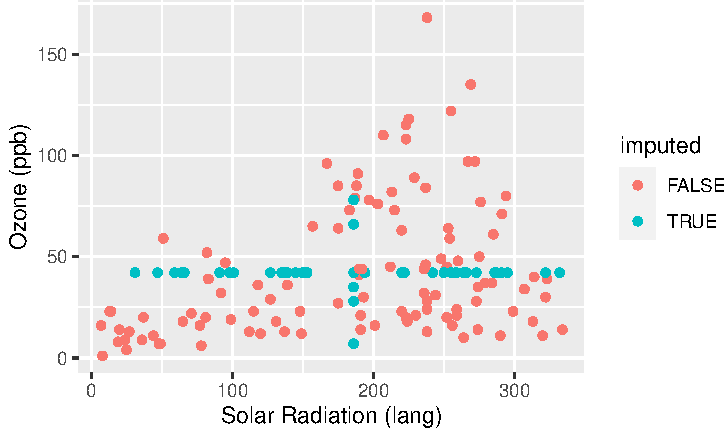
\includegraphics{intro_missing_data_files/figure-pdf/unnamed-chunk-21-2.pdf}

}

\end{figure}

What we see in the above plots is that our imputed observations do not
look like the rest of our data because one (or both) of their values
always is in the exact center. This creates the ``+'' shape. It also
gives the big spike at the mean for the histogram.

\hypertarget{important-aside-namespaces-and-function-collisions}{%
\subsubsection{Important Aside: Namespaces and function
collisions}\label{important-aside-namespaces-and-function-collisions}}

We now need to discuss a sad aspect of R. The short story is, different
packages have functions with the same names and so if you have both
packages loaded you will need to specify which package to use when
calling such a function. You can do this by giving the ``surname'' of
the function at the beginning of the function call (like, I believe, the
Chinese). This comes up because for us the method \texttt{complete()}
exists both in the tidyverse and in mice. In tidyverse,
\texttt{complete()} fills in rows of missing combinations of values. In
mice, \texttt{complete()} gives us a completed dataset after we have
made an imputation call.

It turns out that since we loaded tidyverse first and mice second, the
mice's \texttt{complete()} method is the default. But if we loaded the
packages in the other order, we would get strange errors. To be clear,
we thus tell R to use \texttt{mice} by writing:

\begin{Shaded}
\begin{Highlighting}[]
\NormalTok{  cmp }\OtherTok{=}\NormalTok{ mice}\SpecialCharTok{::}\FunctionTok{complete}\NormalTok{( imp )}
\end{Highlighting}
\end{Shaded}

In general, you can detect such ``namespace collisions'' by noticing
weird error messages all of a sudden when you don't expect them. You can
then type, for example, \texttt{help(\ complete\ )} and it will list all
the different \texttt{complete}s around.

\begin{Shaded}
\begin{Highlighting}[]
  \FunctionTok{help}\NormalTok{( complete )}
\end{Highlighting}
\end{Shaded}

Also when you load a package it will write down what functions are
getting mixed up for you. If you were looking at your R code you would
get something like this:

\begin{verbatim}
tidyr::complete() masks mice::complete()
\end{verbatim}

\hypertarget{regression-imputation}{%
\section{Regression imputation}\label{regression-imputation}}

Regression imputation is half way between mean imputation and multiple
imputation. In regression imputation we predict what values we expect
for anything missing based on the other values of the observation. For
example, if we know that urban/rural is correlated with race, we might
impute a different value for race if we know an observation came from an
urban environment vs.~rural. We do this with regression: we fit a model
predicting each variable using the others and then use that regression
model to predict any missing values.

We can do this manually, but then it gets very hard when multiple
variables are missing for a given observation. The mice package is more
clever: it does variables one at a time, and the cycles around so
everything can get imputed.

\hypertarget{manually}{%
\subsection{Manually}\label{manually}}

Here is how to use other variables to predict missing values.

\begin{Shaded}
\begin{Highlighting}[]
  \FunctionTok{ic}\NormalTok{( airqualitysub )}
\end{Highlighting}
\end{Shaded}

\begin{verbatim}
   Ozone Solar.R Wind Temp Month Day
5     NA      NA 14.3   56     5   5
6     28      NA 14.9   66     5   6
10    NA     194  8.6   69     5  10
\end{verbatim}

\begin{Shaded}
\begin{Highlighting}[]
\NormalTok{  fit }\OtherTok{\textless{}{-}} \FunctionTok{lm}\NormalTok{(Ozone }\SpecialCharTok{\textasciitilde{}}\NormalTok{ Solar.R, }\AttributeTok{data=}\NormalTok{airqualitysub)}

\DocumentationTok{\#\# predict for missing ozone  }
\NormalTok{  need.pred }\OtherTok{=} \FunctionTok{subset}\NormalTok{( airqualitysub, }\FunctionTok{is.na}\NormalTok{( Ozone ) )}
\NormalTok{  need.pred}
\end{Highlighting}
\end{Shaded}

\begin{verbatim}
   Ozone Solar.R Wind Temp Month Day
5     NA      NA 14.3   56     5   5
10    NA     194  8.6   69     5  10
\end{verbatim}

\begin{Shaded}
\begin{Highlighting}[]
\NormalTok{  pred }\OtherTok{\textless{}{-}} \FunctionTok{predict}\NormalTok{(fit, }\AttributeTok{newdata=}\NormalTok{need.pred)}
\NormalTok{  pred}
\end{Highlighting}
\end{Shaded}

\begin{verbatim}
   5   10 
  NA 23.1 
\end{verbatim}

But now we have to merge back in, and we didn't solve for case 5 because
we are missing the variable we would use to predict the other missing
variable. Ick. This is where missing data gets \emph{really} hard (when
we have multiple missing values on multiple variables). So let's quit
now and turn to a package that will handle all of this for us.

\hypertarget{mice}{%
\subsection{Mice}\label{mice}}

To do regression imputation using mice, we simply call the
\texttt{mice()} method:

\begin{Shaded}
\begin{Highlighting}[]
\NormalTok{  imp }\OtherTok{\textless{}{-}} \FunctionTok{mice}\NormalTok{(airquality[,}\DecValTok{1}\SpecialCharTok{:}\DecValTok{2}\NormalTok{], }\AttributeTok{method=}\StringTok{"norm.predict"}\NormalTok{, }\AttributeTok{m=}\DecValTok{1}\NormalTok{, }\AttributeTok{maxit=}\DecValTok{3}\NormalTok{,}\AttributeTok{seed=}\DecValTok{1}\NormalTok{)}
\end{Highlighting}
\end{Shaded}

\begin{verbatim}

 iter imp variable
  1   1  Ozone  Solar.R
  2   1  Ozone  Solar.R
  3   1  Ozone  Solar.R
\end{verbatim}

We have everything! How did it do it? By \emph{chaining equations}.
First we start with mean imputation. Then we use our fit model to
predict for one covariate, and then we use those predicted scores to
predict for the next covariate, and so forth. We cycle back and then
everything is jointly predicting everything else.

The \texttt{complete()} method gives us a complete dataset with
everything imputed. Like so:

\begin{Shaded}
\begin{Highlighting}[]
\NormalTok{  cdat }\OtherTok{=}\NormalTok{ mice}\SpecialCharTok{::}\FunctionTok{complete}\NormalTok{( imp )}
  \FunctionTok{head}\NormalTok{( cdat )}
\end{Highlighting}
\end{Shaded}

\begin{verbatim}
  Ozone Solar.R
1  41.0     190
2  36.0     118
3  12.0     149
4  18.0     313
5  42.7     186
6  28.0     169
\end{verbatim}

\begin{Shaded}
\begin{Highlighting}[]
  \FunctionTok{nrow}\NormalTok{( cdat )}
\end{Highlighting}
\end{Shaded}

\begin{verbatim}
[1] 153
\end{verbatim}

\begin{Shaded}
\begin{Highlighting}[]
  \FunctionTok{nrow}\NormalTok{( airquality )}
\end{Highlighting}
\end{Shaded}

\begin{verbatim}
[1] 153
\end{verbatim}

Next we make a variable of which cases have imputed values and not (any
row with missing data must have been partially imputed.)

\begin{Shaded}
\begin{Highlighting}[]
\NormalTok{  cdat}\SpecialCharTok{$}\NormalTok{imputed }\OtherTok{=} \FunctionTok{ici}\NormalTok{( airquality )}
\end{Highlighting}
\end{Shaded}

And see our results! Compare to mean imputation, above.

\begin{Shaded}
\begin{Highlighting}[]
\FunctionTok{ggplot}\NormalTok{( cdat, }\FunctionTok{aes}\NormalTok{(}\AttributeTok{x=}\NormalTok{Ozone, }\AttributeTok{col=}\NormalTok{imputed) ) }\SpecialCharTok{+}
    \FunctionTok{stat\_bin}\NormalTok{( }\AttributeTok{geom=}\StringTok{"step"}\NormalTok{, }\AttributeTok{position=}\StringTok{"identity"}\NormalTok{,}
              \AttributeTok{breaks=}\FunctionTok{seq}\NormalTok{(}\SpecialCharTok{{-}}\DecValTok{20}\NormalTok{, }\DecValTok{200}\NormalTok{, }\DecValTok{10}\NormalTok{) )}
\end{Highlighting}
\end{Shaded}

\begin{figure}[H]

{\centering \includegraphics{intro_missing_data_files/figure-pdf/unnamed-chunk-28-1.pdf}

}

\end{figure}

\begin{Shaded}
\begin{Highlighting}[]
\FunctionTok{ggplot}\NormalTok{( cdat, }\FunctionTok{aes}\NormalTok{(}\AttributeTok{y=}\NormalTok{Ozone, }\AttributeTok{x=}\NormalTok{Solar.R, }\AttributeTok{col=}\NormalTok{imputed) ) }\SpecialCharTok{+}
    \FunctionTok{geom\_point}\NormalTok{() }\SpecialCharTok{+}
    \FunctionTok{labs}\NormalTok{( }\AttributeTok{y=}\StringTok{"Ozone (ppb)"}\NormalTok{, }\AttributeTok{x=}\StringTok{"Solar Radiation (lang)"}\NormalTok{ )}
\end{Highlighting}
\end{Shaded}

\begin{figure}[H]

{\centering 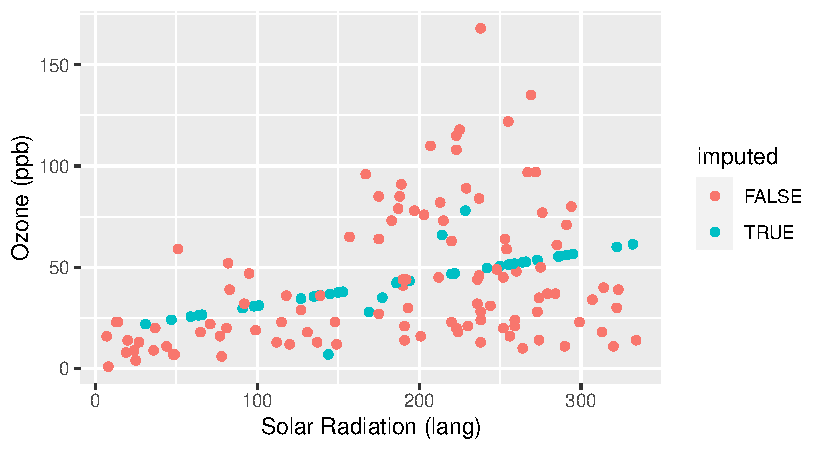
\includegraphics{intro_missing_data_files/figure-pdf/unnamed-chunk-28-2.pdf}

}

\end{figure}

This is better than mean imputation. See how we impute different Ozone
for different Solar Radiation values, taking advantage of the
information of knowing that they are correlated? But it still is obvious
what is mean imputed and what is not. Also, the variance of our imputed
values still does not contain the residual variation around the
predicted values that we would get in real data. We can do one more
enhancement to fix this.

\hypertarget{stochastic-regression-imputation}{%
\subsection{Stochastic regression
imputation}\label{stochastic-regression-imputation}}

We extend regression imputation by randomly drawing observations that
\emph{look like} real ones. See in the two imputations below we get
slightly different values for our imputed data.

Here we do it on our mini-dataset and look at the imputed values for our
observations with missing values only:

\begin{Shaded}
\begin{Highlighting}[]
\NormalTok{  imp }\OtherTok{\textless{}{-}} \FunctionTok{mice}\NormalTok{(airqualitysub[,}\DecValTok{1}\SpecialCharTok{:}\DecValTok{2}\NormalTok{],}\AttributeTok{method=}\StringTok{"norm.nob"}\NormalTok{,}\AttributeTok{m=}\DecValTok{1}\NormalTok{,}\AttributeTok{maxit=}\DecValTok{1}\NormalTok{,}\AttributeTok{seed=}\DecValTok{1}\NormalTok{)}
\end{Highlighting}
\end{Shaded}

\begin{verbatim}

 iter imp variable
  1   1  Ozone  Solar.R
\end{verbatim}

\begin{Shaded}
\begin{Highlighting}[]
\NormalTok{  imp}\SpecialCharTok{$}\NormalTok{imp}
\end{Highlighting}
\end{Shaded}

\begin{verbatim}
$Ozone
       1
5   8.09
10 44.58

$Solar.R
      1
5 181.2
6  83.7
\end{verbatim}

\begin{Shaded}
\begin{Highlighting}[]
\NormalTok{  imp }\OtherTok{\textless{}{-}} \FunctionTok{mice}\NormalTok{(airqualitysub[,}\DecValTok{1}\SpecialCharTok{:}\DecValTok{2}\NormalTok{],}\AttributeTok{method=}\StringTok{"norm.nob"}\NormalTok{,}\AttributeTok{m=}\DecValTok{1}\NormalTok{,}\AttributeTok{maxit=}\DecValTok{1}\NormalTok{,}\AttributeTok{seed=}\DecValTok{4}\NormalTok{)}
\end{Highlighting}
\end{Shaded}

\begin{verbatim}

 iter imp variable
  1   1  Ozone  Solar.R
\end{verbatim}

\begin{Shaded}
\begin{Highlighting}[]
\NormalTok{  imp}\SpecialCharTok{$}\NormalTok{imp}
\end{Highlighting}
\end{Shaded}

\begin{verbatim}
$Ozone
      1
5  34.4
10 31.6

$Solar.R
    1
5 381
6 260
\end{verbatim}

Now let's do it on the full data and look at the imputed values and
compare to our plots above.

\begin{Shaded}
\begin{Highlighting}[]
\NormalTok{  imp }\OtherTok{\textless{}{-}} \FunctionTok{mice}\NormalTok{(airquality[,}\DecValTok{1}\SpecialCharTok{:}\DecValTok{2}\NormalTok{],}\AttributeTok{method=}\StringTok{"norm.nob"}\NormalTok{,}\AttributeTok{m=}\DecValTok{1}\NormalTok{,}\AttributeTok{maxit=}\DecValTok{1}\NormalTok{,}\AttributeTok{seed=}\DecValTok{1}\NormalTok{)}
\end{Highlighting}
\end{Shaded}

\begin{verbatim}

 iter imp variable
  1   1  Ozone  Solar.R
\end{verbatim}

\begin{Shaded}
\begin{Highlighting}[]
\NormalTok{  cdat }\OtherTok{=}\NormalTok{ mice}\SpecialCharTok{::}\FunctionTok{complete}\NormalTok{( imp )}
\NormalTok{  cdat}\SpecialCharTok{$}\NormalTok{imputed }\OtherTok{=} \FunctionTok{ici}\NormalTok{( airquality )}

  \FunctionTok{ggplot}\NormalTok{( cdat, }\FunctionTok{aes}\NormalTok{(}\AttributeTok{x=}\NormalTok{Ozone, }\AttributeTok{col=}\NormalTok{imputed) ) }\SpecialCharTok{+}
    \FunctionTok{stat\_bin}\NormalTok{( }\AttributeTok{geom=}\StringTok{"step"}\NormalTok{, }\AttributeTok{position=}\StringTok{"identity"}\NormalTok{,}
              \AttributeTok{breaks=}\FunctionTok{seq}\NormalTok{(}\SpecialCharTok{{-}}\DecValTok{20}\NormalTok{, }\DecValTok{200}\NormalTok{, }\DecValTok{10}\NormalTok{) )}
\end{Highlighting}
\end{Shaded}

\begin{figure}[H]

{\centering 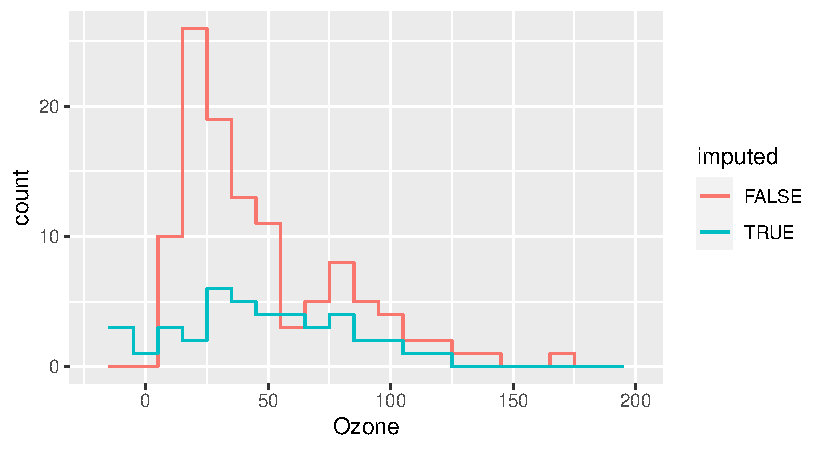
\includegraphics{intro_missing_data_files/figure-pdf/unnamed-chunk-30-1.pdf}

}

\end{figure}

\begin{Shaded}
\begin{Highlighting}[]
  \FunctionTok{ggplot}\NormalTok{( cdat, }\FunctionTok{aes}\NormalTok{(}\AttributeTok{y=}\NormalTok{Ozone, }\AttributeTok{x=}\NormalTok{Solar.R, }\AttributeTok{col=}\NormalTok{imputed) ) }\SpecialCharTok{+}
    \FunctionTok{geom\_point}\NormalTok{() }\SpecialCharTok{+}
    \FunctionTok{labs}\NormalTok{( }\AttributeTok{y=}\StringTok{"Ozone (ppb)"}\NormalTok{, }\AttributeTok{x=}\StringTok{"Solar Radiation (lang)"}\NormalTok{ )}
\end{Highlighting}
\end{Shaded}

\begin{figure}[H]

{\centering 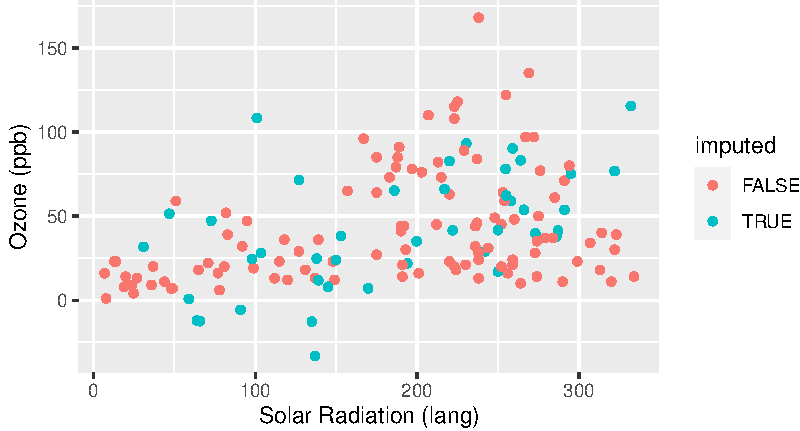
\includegraphics{intro_missing_data_files/figure-pdf/unnamed-chunk-30-2.pdf}

}

\end{figure}

Better, but not perfect. What is better? What is still not perfect?

\hypertarget{multiple-imputation}{%
\section{Multiple imputation}\label{multiple-imputation}}

If missing data is a significant issue in your dataset, then mean or
regression imputation can be a bit too hacky and approximate. In these
contexts, multiple imputation is the way to go.

We do this as follows:

\begin{Shaded}
\begin{Highlighting}[]
\NormalTok{  imp }\OtherTok{\textless{}{-}} \FunctionTok{mice}\NormalTok{(airqualitysub, }\AttributeTok{seed=}\DecValTok{2}\NormalTok{, }\AttributeTok{print=}\ConstantTok{FALSE}\NormalTok{)}
\end{Highlighting}
\end{Shaded}

\begin{verbatim}
Warning: Number of logged events: 1
\end{verbatim}

\begin{Shaded}
\begin{Highlighting}[]
\NormalTok{  imp}
\end{Highlighting}
\end{Shaded}

\begin{verbatim}
Class: mids
Number of multiple imputations:  5 
Imputation methods:
  Ozone Solar.R    Wind    Temp   Month     Day 
  "pmm"   "pmm"      ""      ""      ""      "" 
PredictorMatrix:
        Ozone Solar.R Wind Temp Month Day
Ozone       0       1    1    1     0   1
Solar.R     1       0    1    1     0   1
Wind        1       1    0    1     0   1
Temp        1       1    1    0     0   1
Month       1       1    1    1     0   1
Day         1       1    1    1     0   0
Number of logged events:  1 
  it im dep     meth   out
1  0  0     constant Month
\end{verbatim}

\begin{Shaded}
\begin{Highlighting}[]
\NormalTok{  imp}\SpecialCharTok{$}\NormalTok{imp}
\end{Highlighting}
\end{Shaded}

\begin{verbatim}
$Ozone
    1  2  3  4  5
5  18 41 28 23 23
10 36 18 36 19 28

$Solar.R
    1  2   3  4  5
5 149 99 194 99 19
6 194 19 194 19 19

$Wind
[1] 1 2 3 4 5
<0 rows> (or 0-length row.names)

$Temp
[1] 1 2 3 4 5
<0 rows> (or 0-length row.names)

$Month
[1] 1 2 3 4 5
<0 rows> (or 0-length row.names)

$Day
[1] 1 2 3 4 5
<0 rows> (or 0-length row.names)
\end{verbatim}

See multiple columns of imputed data? (We have 5 here.)

\textbf{First aside:} All variables you'll be using for your model
should be included in the imputation model. Notice we included the full
dataset in \texttt{mice}, not just the variables with missing values.
This way we can account for associations between all the outcome and the
predictors in the model we'll be fitting. Your imputation model can be
more complicated than your model of interest. That is, you can include
additional variables that predict missing values but will not be part of
your final model of interest.

\textbf{Second aside:} All variables in your imputation model should be
in the correct functional form! Quadratic, higher order polynomials and
interaction terms are just another variable that we need to impute.
Although it may seem logical to impute your variables first and then
calculate the interaction or non-linear term, this can lead to bias.

\textbf{Third aside:} The ordering of the variables in the dataset you
are feeding into \texttt{mice} can make a difference in results and
model convergence. Generally, you want to order your variables from
least to most missing. Here, we reorder the variables from least to most
missing, and obtain different results.

\begin{Shaded}
\begin{Highlighting}[]
\NormalTok{  test }\OtherTok{=}\NormalTok{ airqualitysub[,}\FunctionTok{c}\NormalTok{(}\DecValTok{6}\NormalTok{,}\DecValTok{5}\NormalTok{,}\DecValTok{4}\NormalTok{,}\DecValTok{3}\NormalTok{,}\DecValTok{2}\NormalTok{,}\DecValTok{1}\NormalTok{)]}
  \FunctionTok{head}\NormalTok{(test)}
\end{Highlighting}
\end{Shaded}

\begin{verbatim}
  Day Month Temp Wind Solar.R Ozone
1   1     5   67  7.4     190    41
2   2     5   72  8.0     118    36
3   3     5   74 12.6     149    12
4   4     5   62 11.5     313    18
5   5     5   56 14.3      NA    NA
6   6     5   66 14.9      NA    28
\end{verbatim}

\begin{Shaded}
\begin{Highlighting}[]
\NormalTok{  test.imp }\OtherTok{\textless{}{-}} \FunctionTok{mice}\NormalTok{(test, }\AttributeTok{seed=}\DecValTok{2}\NormalTok{, }\AttributeTok{print=}\ConstantTok{FALSE}\NormalTok{)}
\end{Highlighting}
\end{Shaded}

\begin{verbatim}
Warning: Number of logged events: 1
\end{verbatim}

\begin{Shaded}
\begin{Highlighting}[]
\NormalTok{  test.imp}\SpecialCharTok{$}\NormalTok{imp}
\end{Highlighting}
\end{Shaded}

\begin{verbatim}
$Day
[1] 1 2 3 4 5
<0 rows> (or 0-length row.names)

$Month
[1] 1 2 3 4 5
<0 rows> (or 0-length row.names)

$Temp
[1] 1 2 3 4 5
<0 rows> (or 0-length row.names)

$Wind
[1] 1 2 3 4 5
<0 rows> (or 0-length row.names)

$Solar.R
    1   2   3   4   5
5 194 118 194 313 190
6 118 194 118 118 190

$Ozone
    1  2  3  4  5
5  18 23 23 23 41
10 12  8 18 19  8
\end{verbatim}

\textbf{How to get each complete dataset?}

\begin{Shaded}
\begin{Highlighting}[]
\DocumentationTok{\#\# first complete dataset }
\NormalTok{  mice}\SpecialCharTok{::}\FunctionTok{complete}\NormalTok{(imp, }\DecValTok{1}\NormalTok{)}
\end{Highlighting}
\end{Shaded}

\begin{verbatim}
   Ozone Solar.R Wind Temp Month Day
1     41     190  7.4   67     5   1
2     36     118  8.0   72     5   2
3     12     149 12.6   74     5   3
4     18     313 11.5   62     5   4
5     18     149 14.3   56     5   5
6     28     194 14.9   66     5   6
7     23     299  8.6   65     5   7
8     19      99 13.8   59     5   8
9      8      19 20.1   61     5   9
10    36     194  8.6   69     5  10
\end{verbatim}

\begin{Shaded}
\begin{Highlighting}[]
\DocumentationTok{\#\# and our second complete dataset}
\NormalTok{  mice}\SpecialCharTok{::}\FunctionTok{complete}\NormalTok{(imp, }\DecValTok{2}\NormalTok{)}
\end{Highlighting}
\end{Shaded}

\begin{verbatim}
   Ozone Solar.R Wind Temp Month Day
1     41     190  7.4   67     5   1
2     36     118  8.0   72     5   2
3     12     149 12.6   74     5   3
4     18     313 11.5   62     5   4
5     41      99 14.3   56     5   5
6     28      19 14.9   66     5   6
7     23     299  8.6   65     5   7
8     19      99 13.8   59     5   8
9      8      19 20.1   61     5   9
10    18     194  8.6   69     5  10
\end{verbatim}

See how they are different? They were randomly imputed. We basically
used the stochastic regression thing, above, multiple times.

\begin{Shaded}
\begin{Highlighting}[]
\NormalTok{  mice}\SpecialCharTok{::}\FunctionTok{complete}\NormalTok{(imp, }\DecValTok{1}\NormalTok{)[ }\FunctionTok{ici}\NormalTok{(airqualitysub), ]}
\end{Highlighting}
\end{Shaded}

\begin{verbatim}
   Ozone Solar.R Wind Temp Month Day
5     18     149 14.3   56     5   5
6     28     194 14.9   66     5   6
10    36     194  8.6   69     5  10
\end{verbatim}

\begin{Shaded}
\begin{Highlighting}[]
\NormalTok{  mice}\SpecialCharTok{::}\FunctionTok{complete}\NormalTok{(imp, }\DecValTok{2}\NormalTok{)[ }\FunctionTok{ici}\NormalTok{(airqualitysub), ]}
\end{Highlighting}
\end{Shaded}

\begin{verbatim}
   Ozone Solar.R Wind Temp Month Day
5     41      99 14.3   56     5   5
6     28      19 14.9   66     5   6
10    18     194  8.6   69     5  10
\end{verbatim}

On full data:

\begin{Shaded}
\begin{Highlighting}[]
\NormalTok{  imp }\OtherTok{\textless{}{-}} \FunctionTok{mice}\NormalTok{(airquality, }\AttributeTok{seed=}\DecValTok{1}\NormalTok{, }\AttributeTok{print=}\ConstantTok{FALSE}\NormalTok{)}
\end{Highlighting}
\end{Shaded}

Now we estimate for each imputed dataset using the \texttt{with()}
method that, in \texttt{mice}, will do the regression for each completed
dataset. See \texttt{help\ with.mids}.

\begin{Shaded}
\begin{Highlighting}[]
\NormalTok{  fit }\OtherTok{\textless{}{-}} \FunctionTok{with}\NormalTok{(imp, }\FunctionTok{lm}\NormalTok{(Ozone }\SpecialCharTok{\textasciitilde{}}\NormalTok{ Wind }\SpecialCharTok{+}\NormalTok{ Temp }\SpecialCharTok{+}\NormalTok{ Solar.R))}
\NormalTok{  fit}
\end{Highlighting}
\end{Shaded}

\begin{verbatim}
call :
with.mids(data = imp, expr = lm(Ozone ~ Wind + Temp + Solar.R))

call1 :
mice(data = airquality, printFlag = FALSE, seed = 1)

nmis :
  Ozone Solar.R    Wind    Temp   Month     Day 
     37       7       0       0       0       0 

analyses :
[[1]]

Call:
lm(formula = Ozone ~ Wind + Temp + Solar.R)

Coefficients:
(Intercept)         Wind         Temp      Solar.R  
   -66.2402      -2.8219       1.6134       0.0563  


[[2]]

Call:
lm(formula = Ozone ~ Wind + Temp + Solar.R)

Coefficients:
(Intercept)         Wind         Temp      Solar.R  
   -71.2842      -2.9055       1.6749       0.0633  


[[3]]

Call:
lm(formula = Ozone ~ Wind + Temp + Solar.R)

Coefficients:
(Intercept)         Wind         Temp      Solar.R  
   -66.9511      -2.9322       1.6479       0.0543  


[[4]]

Call:
lm(formula = Ozone ~ Wind + Temp + Solar.R)

Coefficients:
(Intercept)         Wind         Temp      Solar.R  
   -33.8480      -3.6628       1.3244       0.0427  


[[5]]

Call:
lm(formula = Ozone ~ Wind + Temp + Solar.R)

Coefficients:
(Intercept)         Wind         Temp      Solar.R  
   -77.4163      -2.7438       1.7264       0.0663  
\end{verbatim}

This can take \emph{any} function call that takes a formula. So
\texttt{glm}, \texttt{lm}, whatever\ldots{} We can then pool the
estimates using the standard theory of combining multiply imputed
datasets. The basic idea is to combine the variation/uncertainty of the
multiple sets with the average uncertainty we would have for each set if
it was truly complete and not imputed.

\begin{Shaded}
\begin{Highlighting}[]
\NormalTok{  tab }\OtherTok{\textless{}{-}} \FunctionTok{summary}\NormalTok{(}\FunctionTok{pool}\NormalTok{(fit))}
  \FunctionTok{colnames}\NormalTok{( tab )}
\end{Highlighting}
\end{Shaded}

\begin{verbatim}
[1] "term"      "estimate"  "std.error" "statistic" "df"        "p.value"  
\end{verbatim}

\begin{Shaded}
\begin{Highlighting}[]
\NormalTok{  tab[,}\FunctionTok{c}\NormalTok{(}\DecValTok{1}\SpecialCharTok{:}\DecValTok{3}\NormalTok{,}\DecValTok{5}\NormalTok{)]}
\end{Highlighting}
\end{Shaded}

\begin{verbatim}
         term estimate std.error   df
1 (Intercept) -63.1480   26.6769 13.8
2        Wind  -3.0132    0.6831 24.0
3        Temp   1.5974    0.2742 19.6
4     Solar.R   0.0566    0.0222 52.4
\end{verbatim}

\textbf{Aside:} You will notice that once we fit our model on the
imputed data, \texttt{with()} returned an object of class \texttt{mira}.
\texttt{Mira} objects can be pooled to get the pooled estimates, whereas
objects of class \texttt{glm}, \texttt{lm}, \texttt{lmer}, etc. cannot
be pooled. You will also notice that you cannot use \texttt{predict}
with a \texttt{mira} object. To use \texttt{predict}, you can stack the
imputed datasets and fit your model on this complete dataset. Parameter
estimates generated by \texttt{pool} are the average of the parameter
estimates from the model fit on each imputed dataset separately. So your
coefficients are fine. However, your SEs will be underestimated. How
underestimated your SEs will be depends, to an extent, on how much data
is missing and whether it is missing at random.

Our old, sad method:

\begin{Shaded}
\begin{Highlighting}[]
\NormalTok{  fit }\OtherTok{\textless{}{-}} \FunctionTok{lm}\NormalTok{(Ozone}\SpecialCharTok{\textasciitilde{}}\NormalTok{Wind}\SpecialCharTok{+}\NormalTok{Temp}\SpecialCharTok{+}\NormalTok{Solar.R,}\AttributeTok{data=}\NormalTok{airquality,}\AttributeTok{na.action=}\NormalTok{na.omit)}
  \FunctionTok{summary}\NormalTok{( fit )}
\end{Highlighting}
\end{Shaded}

\begin{verbatim}

Call:
lm(formula = Ozone ~ Wind + Temp + Solar.R, data = airquality, 
    na.action = na.omit)

Residuals:
   Min     1Q Median     3Q    Max 
-40.48 -14.22  -3.55  10.10  95.62 

Coefficients:
            Estimate Std. Error t value Pr(>|t|)    
(Intercept) -64.3421    23.0547   -2.79   0.0062 ** 
Wind         -3.3336     0.6544   -5.09  1.5e-06 ***
Temp          1.6521     0.2535    6.52  2.4e-09 ***
Solar.R       0.0598     0.0232    2.58   0.0112 *  
---
Signif. codes:  0 '***' 0.001 '**' 0.01 '*' 0.05 '.' 0.1 ' ' 1

Residual standard error: 21.2 on 107 degrees of freedom
  (42 observations deleted due to missingness)
Multiple R-squared:  0.606, Adjusted R-squared:  0.595 
F-statistic: 54.8 on 3 and 107 DF,  p-value: <2e-16
\end{verbatim}

\begin{Shaded}
\begin{Highlighting}[]
  \FunctionTok{round}\NormalTok{(}\FunctionTok{coef}\NormalTok{(}\FunctionTok{summary}\NormalTok{(fit)),}\DecValTok{3}\NormalTok{)}
\end{Highlighting}
\end{Shaded}

\begin{verbatim}
            Estimate Std. Error t value Pr(>|t|)
(Intercept)   -64.34     23.055   -2.79    0.006
Wind           -3.33      0.654   -5.09    0.000
Temp            1.65      0.254    6.52    0.000
Solar.R         0.06      0.023    2.58    0.011
\end{verbatim}

In this case, the missing data estimates are basically the same as the
complete case analysis, it appears. We only had 5\% missing data though.

\hypertarget{extensions}{%
\section{Extensions}\label{extensions}}

\hypertarget{non-continuous-variables}{%
\subsection{Non-continuous variables}\label{non-continuous-variables}}

Everything shown above can easily be extended to non-continuous
variables. The easiest way to do this is using the \texttt{mice}
package. It allows you to specify the type of variable you are imputing,
e.g.~dichotomous or categorical. \texttt{Mice} will automatically detect
and handle non-continuous variables. You can also specify these
variables yourself. Here is an example using \texttt{nhanes} data
(another built-in R dataset).

\begin{Shaded}
\begin{Highlighting}[]
\DocumentationTok{\#\# load data }
  \FunctionTok{data}\NormalTok{(nhanes2)}
  \FunctionTok{head}\NormalTok{(nhanes2)}
\end{Highlighting}
\end{Shaded}

\begin{verbatim}
    age  bmi  hyp chl
1 20-39   NA <NA>  NA
2 40-59 22.7   no 187
3 20-39   NA   no 187
4 60-99   NA <NA>  NA
5 20-39 20.4   no 113
6 60-99   NA <NA> 184
\end{verbatim}

\begin{Shaded}
\begin{Highlighting}[]
\DocumentationTok{\#\# create some missing values for an ordered categorical variable}
\NormalTok{  nhanes2}\SpecialCharTok{$}\NormalTok{age[}\DecValTok{1}\SpecialCharTok{:}\DecValTok{5}\NormalTok{] }\OtherTok{=} \ConstantTok{NA}
  \FunctionTok{head}\NormalTok{(nhanes2) }
\end{Highlighting}
\end{Shaded}

\begin{verbatim}
    age  bmi  hyp chl
1  <NA>   NA <NA>  NA
2  <NA> 22.7   no 187
3  <NA>   NA   no 187
4  <NA>   NA <NA>  NA
5  <NA> 20.4   no 113
6 60-99   NA <NA> 184
\end{verbatim}

\begin{Shaded}
\begin{Highlighting}[]
\DocumentationTok{\#\# impute 5 datasets }
\NormalTok{  imp.cat }\OtherTok{\textless{}{-}} \FunctionTok{mice}\NormalTok{(nhanes2, }\AttributeTok{m =} \DecValTok{5}\NormalTok{, }\AttributeTok{print=}\ConstantTok{FALSE}\NormalTok{)     }
\NormalTok{  full.cat }\OtherTok{=}\NormalTok{ mice}\SpecialCharTok{::}\FunctionTok{complete}\NormalTok{(imp.cat)           }\DocumentationTok{\#\# print the first imputed data set}
  \FunctionTok{head}\NormalTok{(full.cat)}
\end{Highlighting}
\end{Shaded}

\begin{verbatim}
    age  bmi hyp chl
1 40-59 21.7 yes 187
2 40-59 22.7  no 187
3 20-39 27.5  no 187
4 60-99 24.9 yes 218
5 40-59 20.4  no 113
6 60-99 24.9 yes 184
\end{verbatim}

We can check what imputation method \texttt{mice} used for each
variable:

\begin{Shaded}
\begin{Highlighting}[]
\NormalTok{  imp.cat}\SpecialCharTok{$}\NormalTok{method}
\end{Highlighting}
\end{Shaded}

\begin{verbatim}
      age       bmi       hyp       chl 
"polyreg"     "pmm"  "logreg"     "pmm" 
\end{verbatim}

We can see that \texttt{mice} used the \texttt{polyreg} imputation
method for the variable \emph{age}, which means it treated it as an
unordered categorical variable. But this is an ordered variable: higher
values categories signified older age. We can manually force
\texttt{mice} to treat \emph{age} as an ordered categorical variable. We
will keep the imputation methods for the remaining variables the same.

\begin{Shaded}
\begin{Highlighting}[]
\NormalTok{  imp.cat2 }\OtherTok{\textless{}{-}} \FunctionTok{mice}\NormalTok{(nhanes2, }\AttributeTok{meth=}\FunctionTok{c}\NormalTok{(}\StringTok{"polr"}\NormalTok{,}\StringTok{"pmm"}\NormalTok{,}\StringTok{"logreg"}\NormalTok{,}\StringTok{"pmm"}\NormalTok{), }\AttributeTok{m=}\DecValTok{5}\NormalTok{, }\AttributeTok{print=}\ConstantTok{FALSE}\NormalTok{)}
  \FunctionTok{head}\NormalTok{(mice}\SpecialCharTok{::}\FunctionTok{complete}\NormalTok{(imp.cat2, }\DecValTok{1}\NormalTok{))}
\end{Highlighting}
\end{Shaded}

\begin{verbatim}
    age  bmi hyp chl
1 40-59 27.5 yes 184
2 60-99 22.7  no 187
3 60-99 20.4  no 187
4 20-39 35.3  no 184
5 40-59 20.4  no 113
6 60-99 22.7  no 184
\end{verbatim}

\begin{Shaded}
\begin{Highlighting}[]
\NormalTok{  imp.cat2}\SpecialCharTok{$}\NormalTok{method}
\end{Highlighting}
\end{Shaded}

\begin{verbatim}
     age      bmi      hyp      chl 
  "polr"    "pmm" "logreg"    "pmm" 
\end{verbatim}

\hypertarget{multi-level-data}{%
\subsection{Multi-level data}\label{multi-level-data}}

Multilevel data gets more tricky: should we impute taking into account
cluster? How do we do that?

For an initial pass, I would recommend simply doing regression
imputation \emph{ignoring} cluster/grouping, and then adding in that
dummy variable of whether a value is imputed.

\hypertarget{longitudinal-data}{%
\subsection{Longitudinal data}\label{longitudinal-data}}

With longitudinal data we can often use all our data even for
individuals with missing data on the outcome, if we assume data are MAR
(``Missing at Random''). MAR means that conditional on the observed
data, missingness may depend on any observed data, but not on unobserved
data. we explore our missing data on individuals over time and on
outcomes as above to get a sense of whether MAR is a reasonable
assumption or not. Then \texttt{lmer} basically handles the rest for us,
as far as we have enough observations per individual, on average, to
estimate the number of random effects we are trying to estimate. With
respect to missing data on covariates or predictors, you can handle
those with one of the methods described above.

Here we show how to explore missing data in longitudinal analysis using
data on toenail detachment, which you will see in the unit on
generalized MLMs. The data is from a RCT where patients were getting a
different type of drug to prevent toenail detachment (the outcome).

\begin{Shaded}
\begin{Highlighting}[]
\DocumentationTok{\#\# load data}
\NormalTok{  toes }\OtherTok{=}\NormalTok{ foreign}\SpecialCharTok{::}\FunctionTok{read.dta}\NormalTok{( }\StringTok{"data/toenail.dta"}\NormalTok{ )}
\end{Highlighting}
\end{Shaded}

First, let's look at how many times patients were observed.

\begin{Shaded}
\begin{Highlighting}[]
\DocumentationTok{\#\# how many time points per patient?}
  \FunctionTok{table}\NormalTok{( }\FunctionTok{table}\NormalTok{( toes}\SpecialCharTok{$}\NormalTok{patient ) )}
\end{Highlighting}
\end{Shaded}

\begin{verbatim}

  1   2   3   4   5   6   7 
  5   3   7   6  10  39 224 
\end{verbatim}

We have 224 patients observed at all 7 time points, and the rest of the
patients are observed at fewer time points, between 1 and 6.

\begin{Shaded}
\begin{Highlighting}[]
\DocumentationTok{\#\# define function }
\NormalTok{summarise.patient }\OtherTok{=} \ControlFlowTok{function}\NormalTok{( patient ) \{}
\NormalTok{    pat }\OtherTok{=} \FunctionTok{rep}\NormalTok{( }\StringTok{"."}\NormalTok{, }\DecValTok{7}\NormalTok{ )}
\NormalTok{    pat[ patient}\SpecialCharTok{$}\NormalTok{visit ] }\OtherTok{=} \StringTok{\textquotesingle{}X\textquotesingle{}}
    \FunctionTok{paste}\NormalTok{( pat, }\AttributeTok{collapse=}\StringTok{""}\NormalTok{ )}
\NormalTok{\}}
  \DocumentationTok{\#\# For each patient, this code makes a string of "." }
  \DocumentationTok{\#\# then it replaces all dots with an "X" if we have data for that visit}

\DocumentationTok{\#\# summarize missingness  }
\NormalTok{miss }\OtherTok{=}\NormalTok{ toes }\SpecialCharTok{\%\textgreater{}\%} \FunctionTok{group\_by}\NormalTok{( patient ) }\SpecialCharTok{\%\textgreater{}\%}
    \FunctionTok{do}\NormalTok{( }\AttributeTok{pattern =} \FunctionTok{summarise.patient}\NormalTok{(.) ) }\SpecialCharTok{\%\textgreater{}\%}
    \FunctionTok{unnest}\NormalTok{(}\AttributeTok{cols =} \FunctionTok{c}\NormalTok{(pattern))}
  \DocumentationTok{\#\# Group the data by patient }
  \DocumentationTok{\#\# Then use the do() command on each chunk of our dataframe}
  \DocumentationTok{\#\# The "." means "the chunk" (it is a pronoun, essentially).  }
  \DocumentationTok{\#\# This code creates a list of character vectors}
  \DocumentationTok{\#\# The unnest() takes our character vector out of this list made by "do"}

\FunctionTok{head}\NormalTok{( miss )}
\end{Highlighting}
\end{Shaded}

\begin{verbatim}
# A tibble: 6 x 2
  patient pattern
    <dbl> <chr>  
1       1 XXXXXXX
2       2 XXXXXX.
3       3 XXXXXXX
4       4 XXXXXXX
5       6 XXXXXXX
6       7 XXXXXXX
\end{verbatim}

Here we see the different patterns of missing outcomes, i.e., when
patients leave and if they come back. When patients leave and never come
back, regardless of the time point (see lines 4 and 5), we have monotone
missingness.

\begin{Shaded}
\begin{Highlighting}[]
\DocumentationTok{\#\# sort missing patterns in decreasing order}
\DocumentationTok{\#\# starting with no missingness }
\FunctionTok{sort}\NormalTok{( }\FunctionTok{table}\NormalTok{( miss}\SpecialCharTok{$}\NormalTok{pattern ), }\AttributeTok{decreasing=}\ConstantTok{TRUE}\NormalTok{ )}
\end{Highlighting}
\end{Shaded}

\begin{verbatim}

XXXXXXX XXXXX.X XXXX.XX XXX.... X...... XXXXX.. XXXX... XX..... XXX.XXX XXXXXX. 
    224      21      10       6       5       5       4       3       3       3 
XXX.X.. XXXX..X X.XXXXX XX..X.. XX.XXX. XX.XXXX XXX..XX XXX.X.X 
      2       2       1       1       1       1       1       1 
\end{verbatim}

\begin{Shaded}
\begin{Highlighting}[]
\DocumentationTok{\#\# summarize number of data patterns }
\NormalTok{miss }\OtherTok{=}\NormalTok{ miss }\SpecialCharTok{\%\textgreater{}\%} \FunctionTok{group\_by}\NormalTok{( pattern ) }\SpecialCharTok{\%\textgreater{}\%}
    \FunctionTok{summarise}\NormalTok{( }\AttributeTok{n=}\FunctionTok{n}\NormalTok{() )}
\NormalTok{miss }\OtherTok{=} \FunctionTok{arrange}\NormalTok{( miss, }\SpecialCharTok{{-}}\NormalTok{n )}
\NormalTok{miss}
\end{Highlighting}
\end{Shaded}

\begin{verbatim}
# A tibble: 18 x 2
   pattern     n
   <chr>   <int>
 1 XXXXXXX   224
 2 XXXXX.X    21
 3 XXXX.XX    10
 4 XXX....     6
 5 X......     5
 6 XXXXX..     5
 7 XXXX...     4
 8 XX.....     3
 9 XXX.XXX     3
10 XXXXXX.     3
11 XXX.X..     2
12 XXXX..X     2
13 X.XXXXX     1
14 XX..X..     1
15 XX.XXX.     1
16 XX.XXXX     1
17 XXX..XX     1
18 XXX.X.X     1
\end{verbatim}

\begin{Shaded}
\begin{Highlighting}[]
\DocumentationTok{\#\# percent missing data (224 complete cases)}
\DecValTok{224} \SpecialCharTok{/} \FunctionTok{sum}\NormalTok{( miss}\SpecialCharTok{$}\NormalTok{n )}
\end{Highlighting}
\end{Shaded}

\begin{verbatim}
[1] 0.762
\end{verbatim}

\begin{Shaded}
\begin{Highlighting}[]
  \DocumentationTok{\#\# 76\% of patients with complete data}
\end{Highlighting}
\end{Shaded}

Second, we look at patterns of missing outcomes. The outcome here is
toenail detachment.

\begin{Shaded}
\begin{Highlighting}[]
\DocumentationTok{\#\# reshape data to wide }
\NormalTok{  dat.wide }\OtherTok{=} \FunctionTok{reshape}\NormalTok{( toes2, }\AttributeTok{direction=}\StringTok{"wide"}\NormalTok{, }\AttributeTok{v.names=}\StringTok{"outcome"}\NormalTok{,}
                    \AttributeTok{idvar=}\StringTok{"patient"}\NormalTok{, }\AttributeTok{timevar =} \StringTok{"visit"}\NormalTok{ )}
  \FunctionTok{head}\NormalTok{( dat.wide )}
\end{Highlighting}
\end{Shaded}

\begin{verbatim}
   patient treatment           Tx outcome.1 outcome.2 outcome.3 outcome.4
1        1         1 Itraconazole         1         1         1         0
8        2         0  Terbinafine         0         0         1         1
14       3         0  Terbinafine         0         0         0         0
21       4         0  Terbinafine         1         0         0         0
28       6         1 Itraconazole         1         1         1         0
35       7         1 Itraconazole         0         0         0         0
   outcome.5 outcome.6 outcome.7
1          0         0         0
8          0         0        NA
14         0         0         1
21         0         0         0
28         0         0         0
35         1         1         1
\end{verbatim}

\begin{Shaded}
\begin{Highlighting}[]
\DocumentationTok{\#\# looking at missing data with mice package}
  \FunctionTok{md.pattern}\NormalTok{( dat.wide )}
\end{Highlighting}
\end{Shaded}

\begin{figure}[H]

{\centering 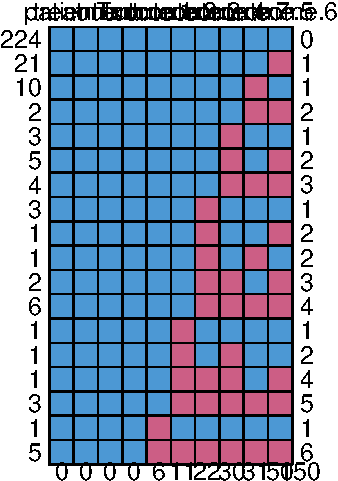
\includegraphics{intro_missing_data_files/figure-pdf/unnamed-chunk-47-1.pdf}

}

\end{figure}

\begin{verbatim}
    patient treatment Tx outcome.1 outcome.2 outcome.3 outcome.4 outcome.7
224       1         1  1         1         1         1         1         1
21        1         1  1         1         1         1         1         1
10        1         1  1         1         1         1         1         1
2         1         1  1         1         1         1         1         1
3         1         1  1         1         1         1         1         0
5         1         1  1         1         1         1         1         0
4         1         1  1         1         1         1         1         0
3         1         1  1         1         1         1         0         1
1         1         1  1         1         1         1         0         1
1         1         1  1         1         1         1         0         1
2         1         1  1         1         1         1         0         0
6         1         1  1         1         1         1         0         0
1         1         1  1         1         1         0         1         1
1         1         1  1         1         1         0         1         0
1         1         1  1         1         1         0         0         0
3         1         1  1         1         1         0         0         0
1         1         1  1         1         0         1         1         1
5         1         1  1         1         0         0         0         0
          0         0  0         0         6        11        22        30
    outcome.5 outcome.6    
224         1         1   0
21          1         0   1
10          0         1   1
2           0         0   2
3           1         1   1
5           1         0   2
4           0         0   3
3           1         1   1
1           1         0   2
1           0         1   2
2           1         0   3
6           0         0   4
1           1         1   1
1           1         1   2
1           1         0   4
3           0         0   5
1           1         1   1
5           0         0   6
           31        50 150
\end{verbatim}

\begin{Shaded}
\begin{Highlighting}[]
\DocumentationTok{\#\# Another way to generating missingness patterns is to create a function}
\DocumentationTok{\#\# This function takes the visits and outcomes and puts a 1 or 0 if there is an}
\DocumentationTok{\#\# outcome and a dot if missing.}
\NormalTok{make.pat }\OtherTok{=} \ControlFlowTok{function}\NormalTok{( visit, outcome ) \{}
\NormalTok{    pat }\OtherTok{=} \FunctionTok{rep}\NormalTok{( }\StringTok{"."}\NormalTok{, }\DecValTok{7}\NormalTok{ )}
\NormalTok{    pat[ visit ] }\OtherTok{=}\NormalTok{ outcome}
    \FunctionTok{paste}\NormalTok{( pat, }\AttributeTok{collapse=}\StringTok{""}\NormalTok{ )}
\NormalTok{\}}

\DocumentationTok{\#\# call our function on all our patients.}
\NormalTok{outcomes }\OtherTok{=}\NormalTok{ toes }\SpecialCharTok{\%\textgreater{}\%} \FunctionTok{group\_by}\NormalTok{( patient ) }\SpecialCharTok{\%\textgreater{}\%}
    \FunctionTok{summarise}\NormalTok{( }\AttributeTok{tx =}\NormalTok{ Tx[[}\DecValTok{1}\NormalTok{]],}
               \AttributeTok{num.obs =} \FunctionTok{n}\NormalTok{(),}
               \AttributeTok{num.detach =} \FunctionTok{sum}\NormalTok{( outcome ),}
               \AttributeTok{out =} \FunctionTok{make.pat}\NormalTok{( visit, outcome ) )}

\FunctionTok{head}\NormalTok{( outcomes, }\DecValTok{20}\NormalTok{ )}
\end{Highlighting}
\end{Shaded}

\begin{verbatim}
# A tibble: 20 x 5
   patient tx           num.obs num.detach out    
     <dbl> <fct>          <int>      <dbl> <chr>  
 1       1 Itraconazole       7          3 1110000
 2       2 Terbinafine        6          2 001100.
 3       3 Terbinafine        7          1 0000001
 4       4 Terbinafine        7          1 1000000
 5       6 Itraconazole       7          3 1110000
 6       7 Itraconazole       7          3 0000111
 7       9 Itraconazole       7          0 0000000
 8      10 Terbinafine        7          0 0000000
 9      11 Itraconazole       7          4 1111000
10      12 Terbinafine        7          3 0100110
11      13 Terbinafine        7          4 1111000
12      15 Itraconazole       6          2 11000.0
13      16 Itraconazole       6          1 0000.10
14      17 Terbinafine        6          4 11110.0
15      18 Terbinafine        6          1 001.000
16      19 Itraconazole       7          0 0000000
17      20 Terbinafine        6          0 000.000
18      21 Itraconazole       3          2 110....
19      22 Terbinafine        7          3 1110000
20      23 Itraconazole       7          0 0000000
\end{verbatim}

\begin{Shaded}
\begin{Highlighting}[]
\DocumentationTok{\#\# how many folks have no detachments?}
\FunctionTok{table}\NormalTok{( outcomes}\SpecialCharTok{$}\NormalTok{num.detach )}
\end{Highlighting}
\end{Shaded}

\begin{verbatim}

  0   1   2   3   4   5   6   7 
163  25  25  31  30   8   4   8 
\end{verbatim}

\begin{Shaded}
\begin{Highlighting}[]
\DecValTok{163} \SpecialCharTok{/} \FunctionTok{nrow}\NormalTok{(outcomes)}
\end{Highlighting}
\end{Shaded}

\begin{verbatim}
[1] 0.554
\end{verbatim}

\begin{Shaded}
\begin{Highlighting}[]
\DocumentationTok{\#\# how many always detached?}
\FunctionTok{sum}\NormalTok{( outcomes}\SpecialCharTok{$}\NormalTok{num.detach }\SpecialCharTok{==}\NormalTok{ outcomes}\SpecialCharTok{$}\NormalTok{num.obs )}
\end{Highlighting}
\end{Shaded}

\begin{verbatim}
[1] 16
\end{verbatim}

\begin{Shaded}
\begin{Highlighting}[]
\DecValTok{16} \SpecialCharTok{/} \FunctionTok{nrow}\NormalTok{(outcomes)}
\end{Highlighting}
\end{Shaded}

\begin{verbatim}
[1] 0.0544
\end{verbatim}

\hypertarget{further-reading}{%
\section{Further reading}\label{further-reading}}

Some further reading on handling missing data. But this is really a
course into itself.

\begin{itemize}
\item
  Gelman \& Hill Chapter 25 has a more detailed discussion of missing
  data imputation.
\item
  White IR, Royston P, Wood AM. Multiple imputation using chained
  equations: issues and guidance for practice. Statistics in Medicine
  2011;30: 377-399.
\item
  Graham, JW, Olchowski, AE, Gilreath, TD, 2007. How Many Imputations
  are Really Needed? Some Practical Clarifications of Multiple
  Imputation Theory 206--213. https://doi.org/10.1007/s11121-007-0070-9
\item
  van Buurin S, Groothuis-Oudshoorn K, MICE: Multivariate Imputation by
  Chained Equations. Journal of Statistical Software. 2011;45(3):1-68.
\item
  Grund S, Lüdtke O, Robitzsch A. Multiple Imputation of Missing Data
  for Multilevel Models: Simulations and Recommendations. DOI:
  10.1177/1094428117703686
\end{itemize}

\hypertarget{appendix-more-about-the-mice-package}{%
\section{Appendix: More about the mice
package}\label{appendix-more-about-the-mice-package}}

The mice package gives back a very complex object that has a lot of
information about how values were imputed, which values were imputed,
and so forth. In the following we unpack the \texttt{imp} variable from
above a bit more.

\textbf{Looking at the imputation object}

In the following code, we look at the object we get back from
\texttt{mice()}. It has lots of parts that we can peek into.

First, the \texttt{imp} list inside of \texttt{imp} stores all of our
newly imputed data. It is itself a list of each variable with their
imputed values:

\begin{Shaded}
\begin{Highlighting}[]
\NormalTok{  imp}\SpecialCharTok{$}\NormalTok{imp}
\end{Highlighting}
\end{Shaded}

\begin{verbatim}
$Ozone
      1   2   3   4   5
5     6  19  14   8  14
10   12  12   7  23  23
25   14  19  14  19  14
26   37  18  32  32  18
27   11   1  18  13  18
32   65  45  13  28  29
33   22  36  12  18  16
34   13  18   1  13  13
35   63  35  45  52  71
36   23  39  20  59  96
37   24  16  12  34  18
39   64 135  85  80  91
42  115  76 115  37  91
43   66 122  78  64 122
45   44  28  45  23  16
46   23  45  46  45  35
52   20  52  63  47  47
53   59  59  48 115  37
54   40  16  35  37  63
55   40  35  48  39  49
56   23  39  59  59  16
57   44  52  40  52  20
58   30  30  27  14  23
59   45  32  16  16  46
60   44  27  34  28  30
61   89  64  80  37  64
65   16  16  14  23  29
72   46  52  65  45  35
75   35  64  71  18  78
83   20  40  71  46  59
84   28  63  37  29  63
102 115  78  78  37  66
103  46  29  31  23  40
107  16  30  13  14  22
115  41  12  44   7  22
119  50  78 122  85  50
150  24  12  27  21  12

$Solar.R
     1   2   3   4   5
5    7 313  82  13 314
6  322 187 222  24 238
11  66 274 139 135 112
27  20  24   7 238 193
96 175 223 284 197 220
97  51 139 274 237  98
98  98 203 220 188 276

$Wind
[1] 1 2 3 4 5
<0 rows> (or 0-length row.names)

$Temp
[1] 1 2 3 4 5
<0 rows> (or 0-length row.names)

$Month
[1] 1 2 3 4 5
<0 rows> (or 0-length row.names)

$Day
[1] 1 2 3 4 5
<0 rows> (or 0-length row.names)
\end{verbatim}

\begin{Shaded}
\begin{Highlighting}[]
  \FunctionTok{str}\NormalTok{( imp}\SpecialCharTok{$}\NormalTok{imp )}
\end{Highlighting}
\end{Shaded}

\begin{verbatim}
List of 6
 $ Ozone  :'data.frame':    37 obs. of  5 variables:
  ..$ 1: int [1:37] 6 12 14 37 11 65 22 13 63 23 ...
  ..$ 2: int [1:37] 19 12 19 18 1 45 36 18 35 39 ...
  ..$ 3: int [1:37] 14 7 14 32 18 13 12 1 45 20 ...
  ..$ 4: int [1:37] 8 23 19 32 13 28 18 13 52 59 ...
  ..$ 5: int [1:37] 14 23 14 18 18 29 16 13 71 96 ...
 $ Solar.R:'data.frame':    7 obs. of  5 variables:
  ..$ 1: int [1:7] 7 322 66 20 175 51 98
  ..$ 2: int [1:7] 313 187 274 24 223 139 203
  ..$ 3: int [1:7] 82 222 139 7 284 274 220
  ..$ 4: int [1:7] 13 24 135 238 197 237 188
  ..$ 5: int [1:7] 314 238 112 193 220 98 276
 $ Wind   :'data.frame':    0 obs. of  5 variables:
  ..$ 1: logi(0) 
  ..$ 2: logi(0) 
  ..$ 3: logi(0) 
  ..$ 4: logi(0) 
  ..$ 5: logi(0) 
 $ Temp   :'data.frame':    0 obs. of  5 variables:
  ..$ 1: logi(0) 
  ..$ 2: logi(0) 
  ..$ 3: logi(0) 
  ..$ 4: logi(0) 
  ..$ 5: logi(0) 
 $ Month  :'data.frame':    0 obs. of  5 variables:
  ..$ 1: logi(0) 
  ..$ 2: logi(0) 
  ..$ 3: logi(0) 
  ..$ 4: logi(0) 
  ..$ 5: logi(0) 
 $ Day    :'data.frame':    0 obs. of  5 variables:
  ..$ 1: logi(0) 
  ..$ 2: logi(0) 
  ..$ 3: logi(0) 
  ..$ 4: logi(0) 
  ..$ 5: logi(0) 
\end{verbatim}

\begin{Shaded}
\begin{Highlighting}[]
  \FunctionTok{str}\NormalTok{( imp}\SpecialCharTok{$}\NormalTok{imp}\SpecialCharTok{$}\NormalTok{Ozone )}
\end{Highlighting}
\end{Shaded}

\begin{verbatim}
'data.frame':   37 obs. of  5 variables:
 $ 1: int  6 12 14 37 11 65 22 13 63 23 ...
 $ 2: int  19 12 19 18 1 45 36 18 35 39 ...
 $ 3: int  14 7 14 32 18 13 12 1 45 20 ...
 $ 4: int  8 23 19 32 13 28 18 13 52 59 ...
 $ 5: int  14 23 14 18 18 29 16 13 71 96 ...
\end{verbatim}

We see that Ozone and Solar.R have imputed values, and the other
variables do not.

Next, we see two missing observations in our original data and then see
the two imputed values for these two missing observations.

\begin{Shaded}
\begin{Highlighting}[]
\NormalTok{  airqualitysub}\SpecialCharTok{$}\NormalTok{Ozone}
\end{Highlighting}
\end{Shaded}

\begin{verbatim}
 [1] 41 36 12 18 NA 28 23 19  8 NA
\end{verbatim}

\begin{Shaded}
\begin{Highlighting}[]
\NormalTok{  imp}\SpecialCharTok{$}\NormalTok{imp}\SpecialCharTok{$}\NormalTok{Ozone[,}\DecValTok{1}\NormalTok{]}
\end{Highlighting}
\end{Shaded}

\begin{verbatim}
 [1]   6  12  14  37  11  65  22  13  63  23  24  64 115  66  44  23  20  59  40
[20]  40  23  44  30  45  44  89  16  46  35  20  28 115  46  16  41  50  24
\end{verbatim}

We can make (the hard way) a vector of Ozone by plugging our missing
values into the original data. But the \texttt{complete()} method,
above, is preferred.

\begin{Shaded}
\begin{Highlighting}[]
\NormalTok{  oz }\OtherTok{=}\NormalTok{ airqualitysub}\SpecialCharTok{$}\NormalTok{Ozone}
\NormalTok{  oz[ }\FunctionTok{is.na}\NormalTok{( oz ) ] }\OtherTok{=}\NormalTok{ imp}\SpecialCharTok{$}\NormalTok{imp}\SpecialCharTok{$}\NormalTok{Ozone[,}\DecValTok{1}\NormalTok{]}
\end{Highlighting}
\end{Shaded}

\begin{verbatim}
Warning in oz[is.na(oz)] = imp$imp$Ozone[, 1]: number of items to replace is
not a multiple of replacement length
\end{verbatim}

\begin{Shaded}
\begin{Highlighting}[]
\NormalTok{  oz}
\end{Highlighting}
\end{Shaded}

\begin{verbatim}
 [1] 41 36 12 18  6 28 23 19  8 12
\end{verbatim}

\textbf{What else is there in \texttt{imp}?}

\begin{Shaded}
\begin{Highlighting}[]
  \FunctionTok{names}\NormalTok{(imp)}
\end{Highlighting}
\end{Shaded}

\begin{verbatim}
 [1] "data"            "imp"             "m"               "where"          
 [5] "blocks"          "call"            "nmis"            "method"         
 [9] "predictorMatrix" "visitSequence"   "formulas"        "post"           
[13] "blots"           "ignore"          "seed"            "iteration"      
[17] "lastSeedValue"   "chainMean"       "chainVar"        "loggedEvents"   
[21] "version"         "date"           
\end{verbatim}

\textbf{What was our imputation method?}

\begin{Shaded}
\begin{Highlighting}[]
\NormalTok{  imp}\SpecialCharTok{$}\NormalTok{method}
\end{Highlighting}
\end{Shaded}

\begin{verbatim}
  Ozone Solar.R    Wind    Temp   Month     Day 
  "pmm"   "pmm"      ""      ""      ""      "" 
\end{verbatim}

Mean imputation for each variable with missing values. Later this will
say other thing.

\textbf{What was used to impute what?}

\begin{Shaded}
\begin{Highlighting}[]
\NormalTok{  imp}\SpecialCharTok{$}\NormalTok{predictorMatrix}
\end{Highlighting}
\end{Shaded}

\begin{verbatim}
        Ozone Solar.R Wind Temp Month Day
Ozone       0       1    1    1     1   1
Solar.R     1       0    1    1     1   1
Wind        1       1    0    1     1   1
Temp        1       1    1    0     1   1
Month       1       1    1    1     0   1
Day         1       1    1    1     1   0
\end{verbatim}

\hypertarget{appendix-the-amelia-package}{%
\section{Appendix: The amelia
package}\label{appendix-the-amelia-package}}

Amelia is another multiple imputation and missing data package. We do
not prefer it, but have some demonstration code in the following, for
reference.

\begin{Shaded}
\begin{Highlighting}[]
  \FunctionTok{library}\NormalTok{(Amelia)}
\end{Highlighting}
\end{Shaded}

For missingness we can make the following:

\begin{Shaded}
\begin{Highlighting}[]
  \FunctionTok{missmap}\NormalTok{(airquality)}
\end{Highlighting}
\end{Shaded}

\begin{figure}[H]

{\centering 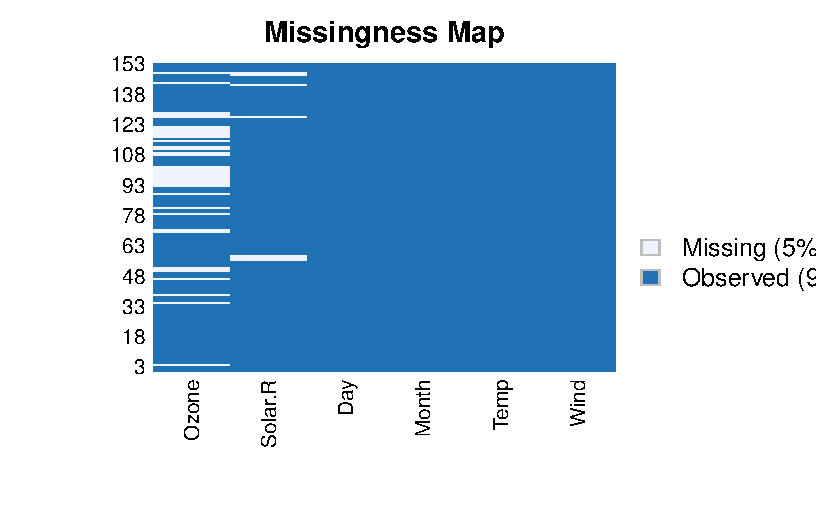
\includegraphics{intro_missing_data_files/figure-pdf/amelia-1.pdf}

}

\end{figure}

Each row of the plot is a row of the data, and missing values are shown
in brown. But ugly! And hard to see any trends in the missingness.

You can use the \texttt{Amelia} package to do mean imputation.

\begin{Shaded}
\begin{Highlighting}[]
  \FunctionTok{library}\NormalTok{(dplyr)}

\DocumentationTok{\#\# exclude variables that do not vary}
\NormalTok{  a.airquality }\OtherTok{=}\NormalTok{ airquality }\SpecialCharTok{\%\textgreater{}\%}\NormalTok{ dplyr}\SpecialCharTok{::}\FunctionTok{select}\NormalTok{(}\SpecialCharTok{{-}}\NormalTok{Month)}

\DocumentationTok{\#\# impute data}
\NormalTok{  a.imp }\OtherTok{\textless{}{-}} \FunctionTok{amelia}\NormalTok{(a.airquality, }\AttributeTok{m=}\DecValTok{5}\NormalTok{)}
\end{Highlighting}
\end{Shaded}

\begin{verbatim}
-- Imputation 1 --

  1  2  3  4  5  6

-- Imputation 2 --

  1  2  3  4  5  6

-- Imputation 3 --

  1  2  3  4  5

-- Imputation 4 --

  1  2  3  4  5  6  7

-- Imputation 5 --

  1  2  3  4  5  6
\end{verbatim}

\begin{Shaded}
\begin{Highlighting}[]
\NormalTok{  a.imp}
\end{Highlighting}
\end{Shaded}

\begin{verbatim}

Amelia output with 5 imputed datasets.
Return code:  1 
Message:  Normal EM convergence. 

Chain Lengths:
--------------
Imputation 1:  6
Imputation 2:  6
Imputation 3:  5
Imputation 4:  7
Imputation 5:  6
\end{verbatim}

We can plot our imputed values against our observed values to check that
they make sense. We will do this for just one of five datasets we just
imputed using \texttt{Amelia}.

\begin{Shaded}
\begin{Highlighting}[]
\DocumentationTok{\#\# put imputed values from the third dataset in an object}
\NormalTok{  one\_imp }\OtherTok{\textless{}{-}}\NormalTok{ a.imp}\SpecialCharTok{$}\NormalTok{imputations[[}\DecValTok{3}\NormalTok{]]}\SpecialCharTok{$}\NormalTok{Ozone}

\DocumentationTok{\#\# make object with observed values }
\DocumentationTok{\#\# from observations without missing Ozone values}
\NormalTok{  obs\_data }\OtherTok{\textless{}{-}}\NormalTok{ a.airquality}\SpecialCharTok{$}\NormalTok{Ozone }
  
\DocumentationTok{\#\# make a plot overlaying observed and imputed values}
  \FunctionTok{hist}\NormalTok{(one\_imp[}\FunctionTok{is.na}\NormalTok{(obs\_data)], }\AttributeTok{prob=}\ConstantTok{TRUE}\NormalTok{, }\AttributeTok{xlab=}\StringTok{"Ozone"}\NormalTok{,}
       \AttributeTok{main=}\StringTok{"Histogram of Imputed Values in 3rd Imputation }\SpecialCharTok{\textbackslash{}n}\StringTok{Compared to Density in Observed Data"}\NormalTok{,}
       \AttributeTok{col=}\StringTok{"cyan"}\NormalTok{, }\AttributeTok{ylim=}\FunctionTok{c}\NormalTok{(}\DecValTok{0}\NormalTok{,}\FloatTok{0.02}\NormalTok{))}
  \FunctionTok{lines}\NormalTok{(}\FunctionTok{density}\NormalTok{(obs\_data[}\SpecialCharTok{!}\FunctionTok{is.na}\NormalTok{(obs\_data)]), }\AttributeTok{col=}\StringTok{"darkblue"}\NormalTok{, }\AttributeTok{lwd=}\DecValTok{2}\NormalTok{)}
\end{Highlighting}
\end{Shaded}

\begin{figure}[H]

{\centering 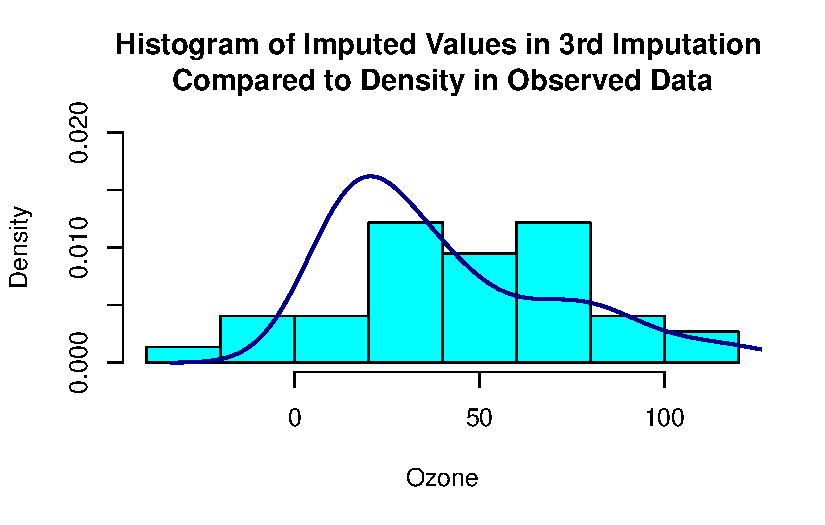
\includegraphics{intro_missing_data_files/figure-pdf/unnamed-chunk-56-1.pdf}

}

\end{figure}

You can also do multiple imputation in \texttt{Amelia}. However,
\texttt{Amelia} does not have an easy way to combine the estimates from
the imputed datasets (no analogue of \texttt{with()} in \texttt{mice}).
You can write a function that fits your model of interest in each
imputed dataset and then use a package like \texttt{mitools} to pool the
estimates and variances.

Much easier to use \texttt{mice}!

\textbf{Aside:} A more important limitation of \texttt{Amelia} is that
the algorithm it uses to impute missing values assumes multivariate
normality, which is often questionable, especially when you have binary
variables.

\part{USING ggPLOT}

\hypertarget{intro-to-ggplot}{%
\chapter{\texorpdfstring{Intro to
\texttt{ggplot}}{Intro to ggplot}}\label{intro-to-ggplot}}

This is a simple script demonstrating some powerful features of a
plotting package \texttt{ggplot2}.

\texttt{ggplot} can initially seem like a nightmare to some, but once
you wrestle it to the ground it is one of the most powerful
visualization tools you might have in your toolbox. Happily, it is
fairly easy to get some basics up and running once you start looking at
the world the way it does. Let's start doing that.

First, \texttt{ggplot} thinks of a plot as a collection of layers
stacked on top of each other. The way this looks in code is a bunch of
weird function calls connected together with \texttt{+}. You read this
series of calls left to right. The first call is always a statement
saying what data you are plotting and what variables you care about. So
before you can even plot, you need to make sure your data are in a nice,
tidy data frame.

Happily, when you load data, it usually is. For example:

\begin{Shaded}
\begin{Highlighting}[]
\NormalTok{dat }\OtherTok{\textless{}{-}} \FunctionTok{read\_dta}\NormalTok{(}\StringTok{"data/hsb.dta"}\NormalTok{) }\SpecialCharTok{|\textgreater{}} 
  \FunctionTok{select}\NormalTok{(}\DecValTok{1}\SpecialCharTok{:}\DecValTok{10}\NormalTok{)}

\FunctionTok{names}\NormalTok{( dat )}
\end{Highlighting}
\end{Shaded}

\begin{verbatim}
 [1] "minority" "female"   "ses"      "mathach"  "size"     "sector"  
 [7] "pracad"   "disclim"  "himinty"  "schoolid"
\end{verbatim}

The easiest full plot to make has two elements. The first gives what
your variables are, and the second says how to plot them:

\begin{Shaded}
\begin{Highlighting}[]
\FunctionTok{ggplot}\NormalTok{(dat, }\FunctionTok{aes}\NormalTok{(}\AttributeTok{y =}\NormalTok{ mathach, }\AttributeTok{x =}\NormalTok{ ses)) }\SpecialCharTok{+} 
  \FunctionTok{geom\_point}\NormalTok{( }\AttributeTok{cex=}\FloatTok{0.5}\NormalTok{)}
\end{Highlighting}
\end{Shaded}

\begin{figure}[H]

{\centering 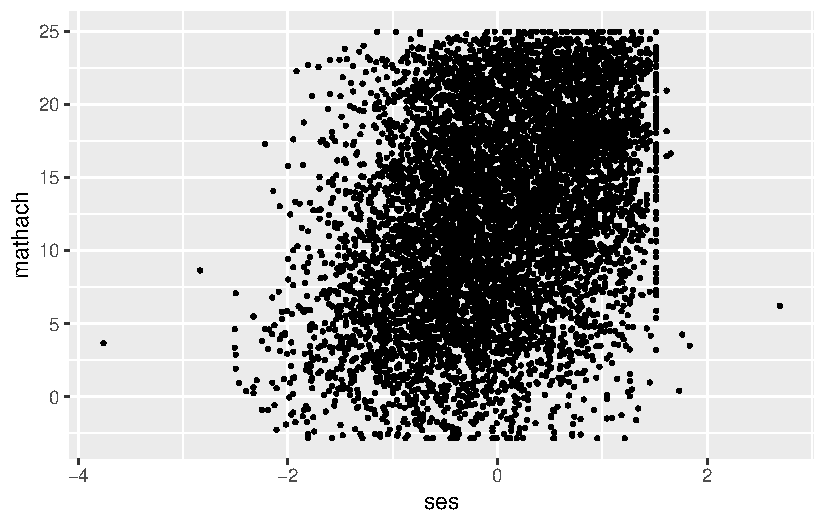
\includegraphics{intro_ggplot_files/figure-pdf/unnamed-chunk-2-1.pdf}

}

\end{figure}

So far, nothing too scary, right? The
\texttt{ggplot(\ dat,\ aes(x=mathach,\ y=ses)\ )} says ``My plot is
going to use \texttt{dat} for my data, and my y-axis is the
\texttt{mathach} variable and my x-axis is \texttt{ses}.'' The
\texttt{aes()} bit is ``aesthetics''--it is a way of tying variables to
different kinds of things you could have on your plot: x location, y
location, color, plotting symbol, and a few other things.

For example:

\begin{Shaded}
\begin{Highlighting}[]
\NormalTok{dat }\OtherTok{\textless{}{-}}\NormalTok{ dat }\SpecialCharTok{|\textgreater{}} 
  \FunctionTok{mutate}\NormalTok{(}\AttributeTok{sector =} \FunctionTok{factor}\NormalTok{(sector, }\AttributeTok{levels=}\FunctionTok{c}\NormalTok{(}\DecValTok{0}\NormalTok{,}\DecValTok{1}\NormalTok{), }\AttributeTok{labels=}\FunctionTok{c}\NormalTok{(}\StringTok{"public"}\NormalTok{,}\StringTok{"catholic"}\NormalTok{)),}
         \AttributeTok{minority =} \FunctionTok{factor}\NormalTok{(minority, }\AttributeTok{labels=}\FunctionTok{c}\NormalTok{(}\StringTok{"non{-}minority"}\NormalTok{,}\StringTok{"minority"}\NormalTok{)))}

\FunctionTok{ggplot}\NormalTok{( dat, }\FunctionTok{aes}\NormalTok{(}\AttributeTok{y=}\NormalTok{mathach, }\AttributeTok{x=}\NormalTok{ses, }\AttributeTok{col=}\NormalTok{sector, }\AttributeTok{pch=}\NormalTok{minority) ) }\SpecialCharTok{+} 
  \FunctionTok{geom\_point}\NormalTok{()}
\end{Highlighting}
\end{Shaded}

\begin{figure}[H]

{\centering 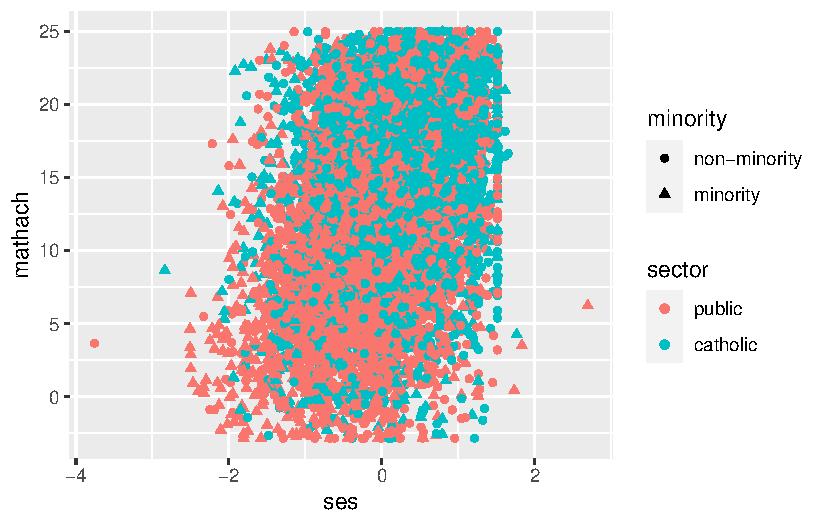
\includegraphics{intro_ggplot_files/figure-pdf/unnamed-chunk-3-1.pdf}

}

\end{figure}

Note that \texttt{ggplot} wants the data frame to be neatly put
together, including that categorical variables are listed as factors.
This is why we convert the dummy \texttt{sector} to a factor above. Once
you do this, however, it will label things in a nice way.

\hypertarget{summarizing}{%
\section{Summarizing}\label{summarizing}}

You can also automatically add various statistical summaries, such as
simple regression lines:

\begin{Shaded}
\begin{Highlighting}[]
\FunctionTok{ggplot}\NormalTok{( dat, }\FunctionTok{aes}\NormalTok{(}\AttributeTok{y=}\NormalTok{mathach, }\AttributeTok{x=}\NormalTok{ses, }\AttributeTok{col=}\NormalTok{sector ) ) }\SpecialCharTok{+} 
    \FunctionTok{geom\_point}\NormalTok{() }\SpecialCharTok{+} 
    \FunctionTok{stat\_smooth}\NormalTok{( }\AttributeTok{method=}\StringTok{"lm"}\NormalTok{, }\AttributeTok{se =} \ConstantTok{FALSE}\NormalTok{ )}
\end{Highlighting}
\end{Shaded}

\begin{verbatim}
`geom_smooth()` using formula = 'y ~ x'
\end{verbatim}

\begin{figure}[H]

{\centering 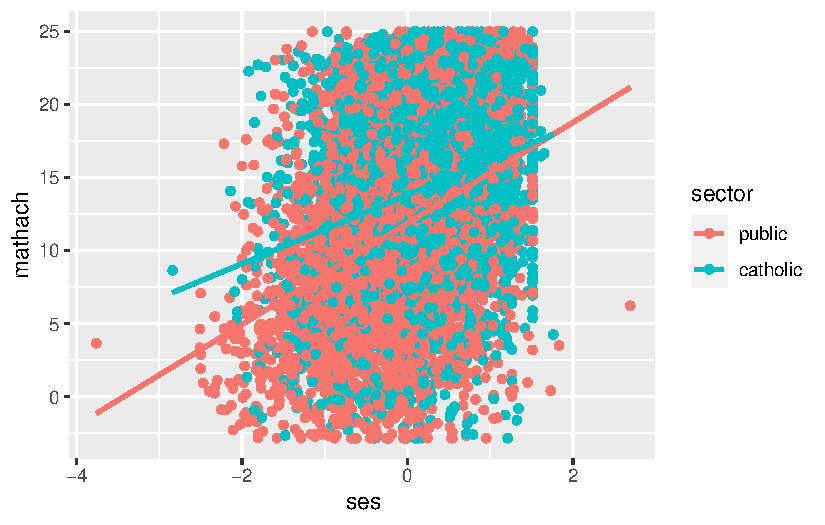
\includegraphics{intro_ggplot_files/figure-pdf/unnamed-chunk-4-1.pdf}

}

\end{figure}

Notice how it automatically realized you have two subgroups of data
defined by sector. It gives you a regression line for each group.

The elements of the plot are stacked, and if you remove one of the
elements, it will not appear:

\begin{Shaded}
\begin{Highlighting}[]
\FunctionTok{ggplot}\NormalTok{( dat, }\FunctionTok{aes}\NormalTok{(}\AttributeTok{y=}\NormalTok{mathach, }\AttributeTok{x=}\NormalTok{ses, }\AttributeTok{col=}\NormalTok{sector ) ) }\SpecialCharTok{+} 
  \FunctionTok{stat\_smooth}\NormalTok{( }\AttributeTok{method=}\StringTok{"lm"}\NormalTok{ )}
\end{Highlighting}
\end{Shaded}

\begin{verbatim}
`geom_smooth()` using formula = 'y ~ x'
\end{verbatim}

\begin{figure}[H]

{\centering 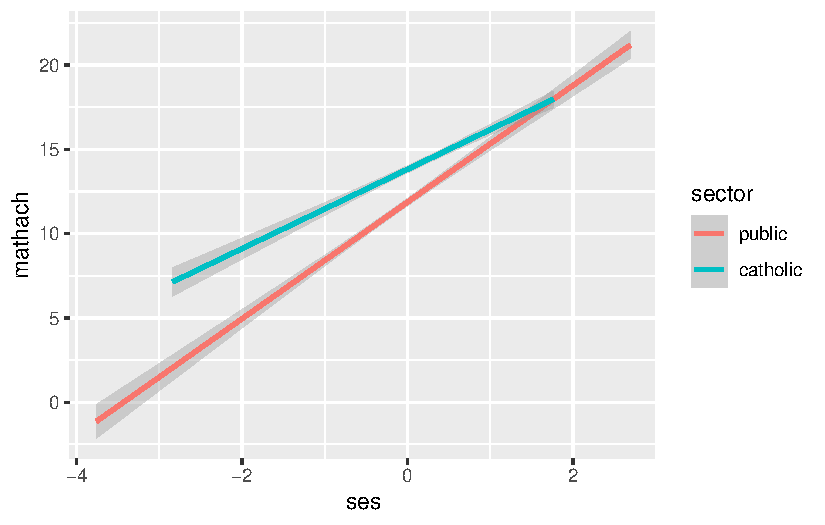
\includegraphics{intro_ggplot_files/figure-pdf/unnamed-chunk-5-1.pdf}

}

\end{figure}

Here we also added some uncertainty bars around the regression lines by
not saying \texttt{se\ =\ FALSE}. (Including uncertainty is the
default.)

\hypertarget{grouping}{%
\section{Grouping}\label{grouping}}

Combining these ideas we can make a trend line for each school:

\begin{Shaded}
\begin{Highlighting}[]
\NormalTok{my.plot }\OtherTok{=} \FunctionTok{ggplot}\NormalTok{( dat, }\FunctionTok{aes}\NormalTok{(}\AttributeTok{y=}\NormalTok{mathach, }\AttributeTok{x=}\NormalTok{ses, }\AttributeTok{col=}\NormalTok{sector, }\AttributeTok{group=}\NormalTok{schoolid ) ) }\SpecialCharTok{+} 
    \FunctionTok{stat\_smooth}\NormalTok{( }\AttributeTok{method=}\StringTok{"lm"}\NormalTok{, }\AttributeTok{se =} \ConstantTok{FALSE}\NormalTok{ )}

\NormalTok{my.plot}
\end{Highlighting}
\end{Shaded}

\begin{verbatim}
`geom_smooth()` using formula = 'y ~ x'
\end{verbatim}

\begin{figure}[H]

{\centering 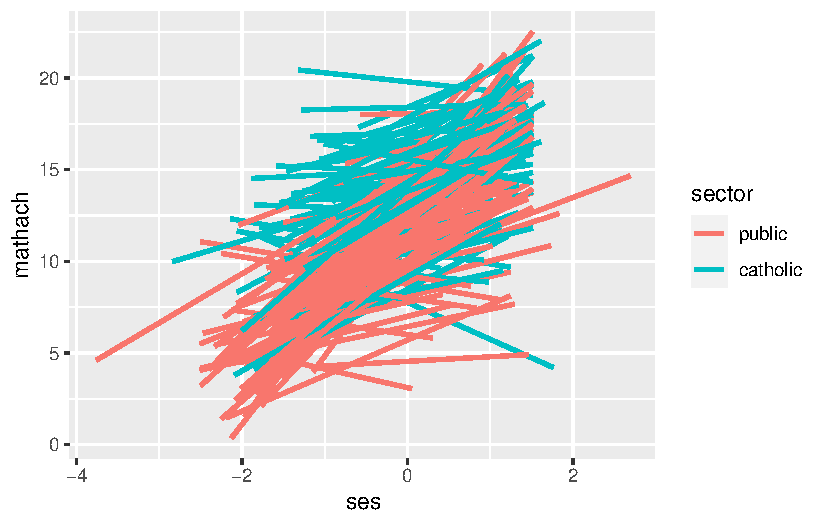
\includegraphics{intro_ggplot_files/figure-pdf/unnamed-chunk-6-1.pdf}

}

\end{figure}

The trendlines automatically extend to the limits of the data they are
run on, hence the different lengths.

Also, notice we ``saved'' the plot in the variable \texttt{my.plot}.
Only when we ``print'' the plot will the plot appear on your display.
When we type the name of a variable, it prints. Once you have a plot
stored in a variable you can augment it very easily.

As you may now realize, \texttt{ggplot2} is very, very powerful.

\hypertarget{customization}{%
\section{Customization}\label{customization}}

We next show some other things you can do. For example, you can make
lots of little plots:

\begin{Shaded}
\begin{Highlighting}[]
\NormalTok{my.plot }\SpecialCharTok{+} 
  \FunctionTok{facet\_grid}\NormalTok{( }\SpecialCharTok{\textasciitilde{}}\NormalTok{ female ) }\SpecialCharTok{+} 
    \FunctionTok{ggtitle}\NormalTok{(}\StringTok{"School{-}level trend lines for their male and female students"}\NormalTok{) }\SpecialCharTok{+}
    \FunctionTok{labs}\NormalTok{(}\AttributeTok{x=}\StringTok{"SES"}\NormalTok{,}\AttributeTok{y=}\StringTok{"Math Achievement"}\NormalTok{) }
\end{Highlighting}
\end{Shaded}

\begin{verbatim}
`geom_smooth()` using formula = 'y ~ x'
\end{verbatim}

\begin{figure}[H]

{\centering 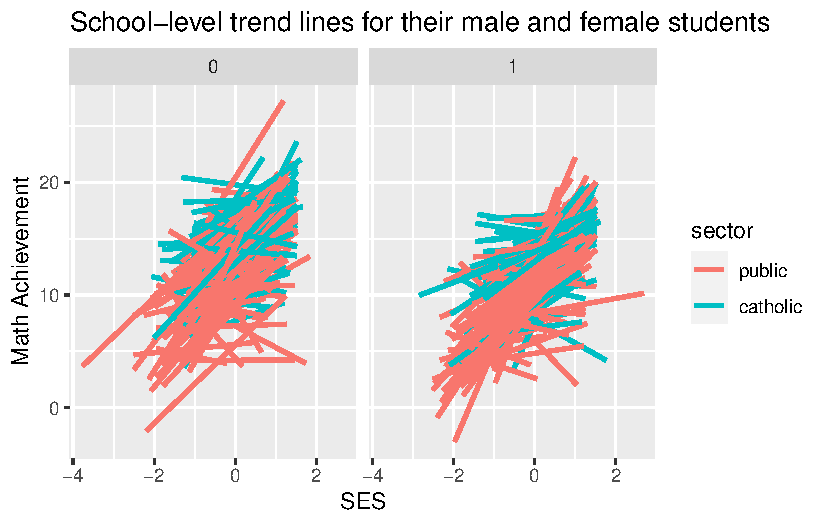
\includegraphics{intro_ggplot_files/figure-pdf/unnamed-chunk-7-1.pdf}

}

\end{figure}

Or,

\begin{Shaded}
\begin{Highlighting}[]
\CommentTok{\# random subset of schoolid}
\NormalTok{sch }\OtherTok{\textless{}{-}} \FunctionTok{sample}\NormalTok{( }\FunctionTok{unique}\NormalTok{( dat}\SpecialCharTok{$}\NormalTok{schoolid ), }\DecValTok{6}\NormalTok{ )}

\CommentTok{\# pipe into ggplot }
\NormalTok{my.six.plot }\OtherTok{\textless{}{-}}\NormalTok{ dat }\SpecialCharTok{|\textgreater{}} 
  \FunctionTok{filter}\NormalTok{(schoolid }\SpecialCharTok{\%in\%}\NormalTok{ sch) }\SpecialCharTok{|\textgreater{}} 
  \FunctionTok{ggplot}\NormalTok{(}\FunctionTok{aes}\NormalTok{(}\AttributeTok{y=}\NormalTok{mathach, }\AttributeTok{x=}\NormalTok{ses, }\AttributeTok{col=}\NormalTok{sector ) ) }\SpecialCharTok{+} 
    \FunctionTok{facet\_wrap}\NormalTok{( }\SpecialCharTok{\textasciitilde{}}\NormalTok{ schoolid, }\AttributeTok{ncol=}\DecValTok{3}\NormalTok{ ) }\SpecialCharTok{+} 
    \FunctionTok{geom\_point}\NormalTok{() }\SpecialCharTok{+} \FunctionTok{stat\_smooth}\NormalTok{( }\AttributeTok{method=}\StringTok{"lm"}\NormalTok{ )}

\NormalTok{my.six.plot}
\end{Highlighting}
\end{Shaded}

\begin{verbatim}
`geom_smooth()` using formula = 'y ~ x'
\end{verbatim}

\begin{figure}[H]

{\centering 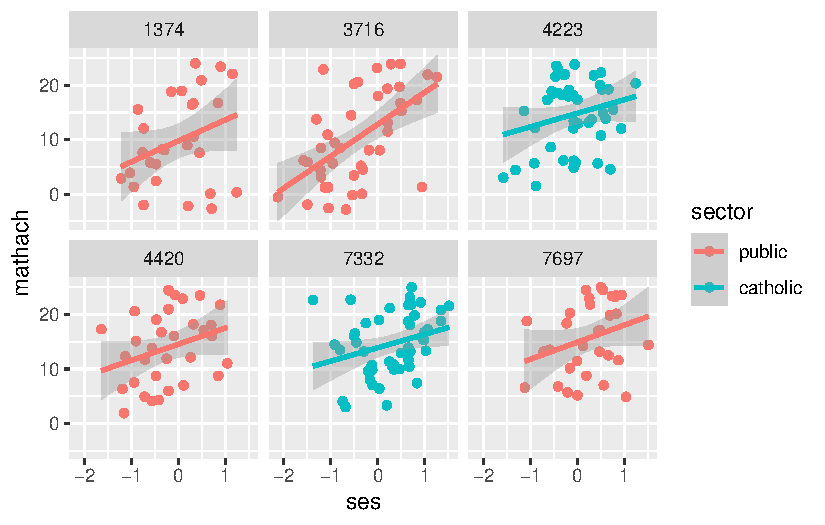
\includegraphics{intro_ggplot_files/figure-pdf/unnamed-chunk-8-1.pdf}

}

\end{figure}

Also shown are adding titles.

\hypertarget{themes}{%
\section{Themes}\label{themes}}

You can very quickly change the entire presentation of your plot using
\texttt{themes}. There are pre-packaged ones, and you can make your own
that you use over and over. Here we set up a theme to be used moving
forward

\begin{Shaded}
\begin{Highlighting}[]
\FunctionTok{library}\NormalTok{( ggthemes )}
\NormalTok{my\_t }\OtherTok{=} \FunctionTok{theme\_calc}\NormalTok{() }\SpecialCharTok{+} \FunctionTok{theme}\NormalTok{( }\AttributeTok{legend.position=}\StringTok{"bottom"}\NormalTok{, }
                             \AttributeTok{legend.direction=}\StringTok{"horizontal"}\NormalTok{, }
                             \AttributeTok{legend.key.width=}\FunctionTok{unit}\NormalTok{(}\DecValTok{1}\NormalTok{,}\StringTok{"cm"}\NormalTok{)  )}
\FunctionTok{theme\_set}\NormalTok{( my\_t )}
\end{Highlighting}
\end{Shaded}

Compare the same plot from above, now with a new theme.

\begin{Shaded}
\begin{Highlighting}[]
\NormalTok{my.six.plot}
\end{Highlighting}
\end{Shaded}

\begin{verbatim}
`geom_smooth()` using formula = 'y ~ x'
\end{verbatim}

\begin{figure}[H]

{\centering 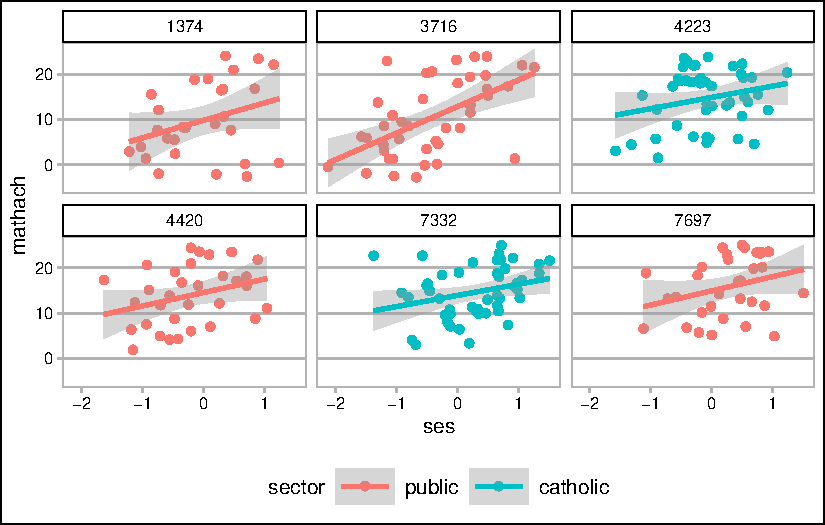
\includegraphics{intro_ggplot_files/figure-pdf/unnamed-chunk-10-1.pdf}

}

\end{figure}

Cool, no?

\hypertarget{next-steps}{%
\section{Next steps}\label{next-steps}}

There is a lot of information out there on \texttt{ggplot} and my best
advice is to find code examples, and then modify them as needed. There
are tutorials and blogs that walk through building plots (search for
``ggplot tutorial'' for example), but seeing examples seems to be the
best way to learn the stuff. For example, you could use the above code
for your project one quite readily. And don't be afraid to ask how to
modify plots on Piazza!

In particular, check out the excellent \href{http://r4ds.had.co.nz}{``R
for Data Science'\,' textbook}. It extensively uses ggplot, starting
\href{http://r4ds.had.co.nz/data-visualisation.html}{here}.

\hypertarget{simple-tables-plots-and-model-diagnostics}{%
\chapter{Simple tables, plots, and model
diagnostics}\label{simple-tables-plots-and-model-diagnostics}}

In this document we give a few simple plots and summary tables that may
be useful for final projects and other things as well. This includes a
few simple model diagnostic plots to check for extreme outliers and
whatnot.

It is a bit of a hodge-podge, but skimming to get some ideas is
definitely worthwhile.

\hypertarget{national-youth-survey-example}{%
\section{National Youth Survey
Example}\label{national-youth-survey-example}}

Our running example is the National Youth Survey (NYS) data as described
in Raudenbush and Bryk, page 190. This data comes from a survey in which
the same students were asked yearly about their acceptance of 9
``deviant'' behaviors (such as smoking marijuana, stealing, etc.). The
study began in 1976, and followed two cohorts of children, starting at
ages 11 and 14 respectively. We will analyze the first 5 years of data.

At each time point, we have measures of:

\begin{itemize}
\tightlist
\item
  \texttt{ATTIT}, the attitude towards deviance, with higher numbers
  implying higher tolerance for deviant behaviors.
\item
  \texttt{EXPO}, the ``exposure'', based on asking the children how many
  friends they had who had engaged in each of the ``deviant'' behaviors.
\end{itemize}

Both of these variables have been transformed to a logarithmic scale to
reduce skew.

For each student, we have:

\begin{itemize}
\tightlist
\item
  Gender (binary)
\item
  Minority status (binary)
\item
  Family income, in units of \$10K (this can be either categorical or
  continuous).
\end{itemize}

\hypertarget{getting-the-data-ready}{%
\subsection{Getting the data ready}\label{getting-the-data-ready}}

We'll focus on the first cohort, from ages 11-15. First, let's read the
data. Note that this data frame is in ``wide format''. That is, there is
only one row for each student, with all the different observations for
that student in different columns of that one row.

\begin{Shaded}
\begin{Highlighting}[]
\NormalTok{nyswide }\OtherTok{\textless{}{-}} \FunctionTok{read\_csv}\NormalTok{(}\StringTok{"data/nyswide.csv"}\NormalTok{)}
\FunctionTok{head}\NormalTok{(nyswide)}
\end{Highlighting}
\end{Shaded}

\begin{verbatim}
# A tibble: 6 x 14
     ID ATTIT.11 EXPO.11 ATTIT.12 EXPO.12 ATTIT.13 EXPO.13 ATTIT.14 EXPO.14
  <dbl>    <dbl>   <dbl>    <dbl>   <dbl>    <dbl>   <dbl>    <dbl>   <dbl>
1     3     0.11   -0.37     0.2    -0.27     0      -0.37     0      -0.27
2     8     0.29    0.42     0.29    0.2      0.11    0.42     0.51    0.2 
3     9     0.8     0.47     0.58    0.52     0.64    0.2      0.75    0.47
4    15     0.44    0.07     0.44    0.32     0.89    0.47     0.75    0.26
5    33     0.2    -0.27     0.64   -0.27     0.69   -0.27    NA      NA   
6    45     0.11    0.26     0.37   -0.17     0.37    0.14     0.37    0.14
# i 5 more variables: ATTIT.15 <dbl>, EXPO.15 <dbl>, FEMALE <dbl>,
#   MINORITY <dbl>, INCOME <dbl>
\end{verbatim}

For our purposes, we want it in ``long format'', i.e.~each student has
multiple rows for the different observations. The
\texttt{pivot\_longer()} command does this for us.

\begin{Shaded}
\begin{Highlighting}[]
\NormalTok{nys1 }\OtherTok{\textless{}{-}}\NormalTok{ nyswide }\SpecialCharTok{|\textgreater{}} 
  \FunctionTok{pivot\_longer}\NormalTok{(ATTIT}\FloatTok{.11}\SpecialCharTok{:}\NormalTok{EXPO}\FloatTok{.15}\NormalTok{, }\AttributeTok{names\_to =} \StringTok{"score"}\NormalTok{) }\SpecialCharTok{|\textgreater{}} 
  \FunctionTok{mutate}\NormalTok{(}\AttributeTok{outcome =} \FunctionTok{word}\NormalTok{(score, }\DecValTok{1}\NormalTok{, }\DecValTok{1}\NormalTok{, }\AttributeTok{sep =} \StringTok{"}\SpecialCharTok{\textbackslash{}\textbackslash{}}\StringTok{."}\NormalTok{),}
         \AttributeTok{age =} \FunctionTok{as.numeric}\NormalTok{(}\FunctionTok{word}\NormalTok{(score, }\DecValTok{2}\NormalTok{, }\DecValTok{2}\NormalTok{, }\AttributeTok{sep =} \StringTok{"}\SpecialCharTok{\textbackslash{}\textbackslash{}}\StringTok{."}\NormalTok{)),}
         \AttributeTok{age\_fac =} \FunctionTok{factor}\NormalTok{(age)) }\SpecialCharTok{|\textgreater{}} 
  \FunctionTok{select}\NormalTok{(}\SpecialCharTok{{-}}\NormalTok{score) }\SpecialCharTok{|\textgreater{}} 
  \FunctionTok{pivot\_wider}\NormalTok{(}\AttributeTok{names\_from =}\NormalTok{ outcome) }\SpecialCharTok{|\textgreater{}} 
  \CommentTok{\# drop missing ATTIT values}
  \FunctionTok{drop\_na}\NormalTok{(ATTIT)}

\FunctionTok{head}\NormalTok{( nys1 )}
\end{Highlighting}
\end{Shaded}

\begin{verbatim}
# A tibble: 6 x 8
     ID FEMALE MINORITY INCOME   age age_fac ATTIT  EXPO
  <dbl>  <dbl>    <dbl>  <dbl> <dbl> <fct>   <dbl> <dbl>
1     3      1        0      3    11 11       0.11 -0.37
2     3      1        0      3    12 12       0.2  -0.27
3     3      1        0      3    13 13       0    -0.37
4     3      1        0      3    14 14       0    -0.27
5     3      1        0      3    15 15       0.11 -0.17
6     8      0        0      4    11 11       0.29  0.42
\end{verbatim}

Just to get a sense of the data, let's plot each age as a boxplot

\begin{Shaded}
\begin{Highlighting}[]
  \FunctionTok{ggplot}\NormalTok{(nys1, }\FunctionTok{aes}\NormalTok{(age\_fac, ATTIT)) }\SpecialCharTok{+}
    \FunctionTok{geom\_boxplot}\NormalTok{() }\SpecialCharTok{+} 
    \FunctionTok{labs}\NormalTok{(}\AttributeTok{title =} \StringTok{"Boxplot of attitude towards deviance by age"}\NormalTok{, }
         \AttributeTok{x =} \StringTok{"Age"}\NormalTok{, }\AttributeTok{y =} \StringTok{"Attitude towards deviance"}\NormalTok{)}
\end{Highlighting}
\end{Shaded}

\begin{figure}[H]

{\centering \includegraphics{summary_plots_files/figure-pdf/unnamed-chunk-3-1.pdf}

}

\end{figure}

\emph{Note:} The boxplot's ``x'' variable is the group. You get one box
per group. The ``y'' variable is the data we are making boxplots of.

Note some features of the data:

\begin{itemize}
\tightlist
\item
  First, we see that \texttt{ATTIT} goes up over time.
\item
  Second, we see the variation of points also goes up over time. This is
  evidence of heteroskedasticity.
\end{itemize}

If we plot individual lines we have:

\begin{Shaded}
\begin{Highlighting}[]
\NormalTok{nys1 }\SpecialCharTok{|\textgreater{}} 
  \FunctionTok{drop\_na}\NormalTok{() }\SpecialCharTok{|\textgreater{}} 
  \FunctionTok{ggplot}\NormalTok{(}\FunctionTok{aes}\NormalTok{(age, ATTIT, }\AttributeTok{group=}\NormalTok{ID)) }\SpecialCharTok{+}
    \FunctionTok{geom\_line}\NormalTok{(}\AttributeTok{alpha=}\FloatTok{0.2}\NormalTok{, }\AttributeTok{position =} \StringTok{"jitter"}\NormalTok{) }\SpecialCharTok{+} 
    \FunctionTok{labs}\NormalTok{(}\AttributeTok{title =} \StringTok{"Individual trajectories of attitude towards deviance over time"}\NormalTok{,}
         \AttributeTok{x =} \StringTok{"Age"}\NormalTok{,}
         \AttributeTok{y =}\StringTok{"Attitude towards deviance"}\NormalTok{)}
\end{Highlighting}
\end{Shaded}

\begin{figure}[H]

{\centering 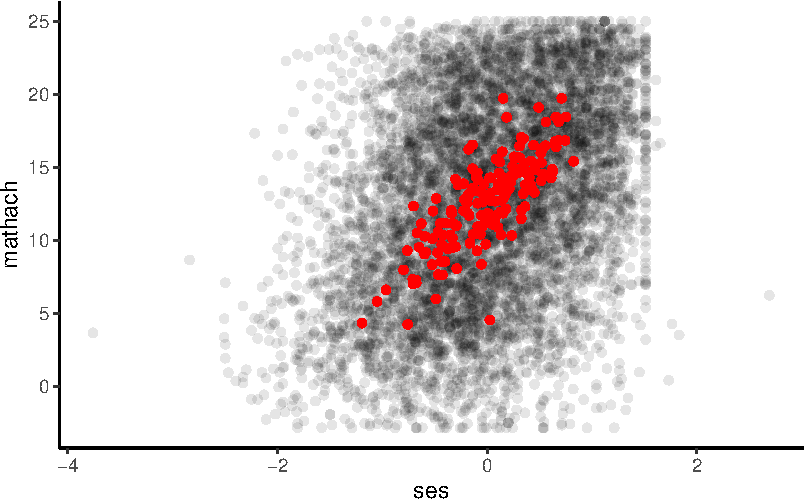
\includegraphics{summary_plots_files/figure-pdf/unnamed-chunk-4-1.pdf}

}

\end{figure}

Note how we have correlation of residuals: some students have
systematically lower trajectories and some students have systematically
higher trajectories (although there is a lot of bouncing around).

\hypertarget{tabulating-data-categorical-variables}{%
\section{Tabulating data (Categorical
variables)}\label{tabulating-data-categorical-variables}}

We can tabulate data as so:

\begin{Shaded}
\begin{Highlighting}[]
\FunctionTok{table}\NormalTok{(nys1}\SpecialCharTok{$}\NormalTok{age)}
\end{Highlighting}
\end{Shaded}

\begin{verbatim}

 11  12  13  14  15 
202 209 230 220 218 
\end{verbatim}

or

\begin{Shaded}
\begin{Highlighting}[]
\FunctionTok{table}\NormalTok{(nys1}\SpecialCharTok{$}\NormalTok{MINORITY, nys1}\SpecialCharTok{$}\NormalTok{age)}
\end{Highlighting}
\end{Shaded}

\begin{verbatim}
   
     11  12  13  14  15
  0 159 165 182 175 175
  1  43  44  48  45  43
\end{verbatim}

Interestingly, we have more observations for later ages.

We can make ``proportion tables'' as well:

\begin{Shaded}
\begin{Highlighting}[]
\FunctionTok{prop.table}\NormalTok{( }\FunctionTok{table}\NormalTok{( nys1}\SpecialCharTok{$}\NormalTok{MINORITY, nys1}\SpecialCharTok{$}\NormalTok{INCOME  ), }\AttributeTok{margin=}\DecValTok{1}\NormalTok{ )}
\end{Highlighting}
\end{Shaded}

\begin{verbatim}
   
          1       2       3       4       5       6       7       8       9
  0 0.06075 0.13551 0.18341 0.18107 0.14369 0.10981 0.06893 0.05257 0.00935
  1 0.28251 0.41704 0.12556 0.05830 0.05830 0.02242 0.01345 0.00000 0.00000
   
         10
  0 0.05491
  1 0.02242
\end{verbatim}

The margin determines what adds up to 100\%.

\hypertarget{summary-stats-continuous-variables}{%
\section{Summary stats (continuous
variables)}\label{summary-stats-continuous-variables}}

The \texttt{tableone} package is useful:

\begin{Shaded}
\begin{Highlighting}[]
  \FunctionTok{library}\NormalTok{(tableone)}
  
\CommentTok{\# sample mean  }
  \FunctionTok{CreateTableOne}\NormalTok{(}\AttributeTok{data =}\NormalTok{ nys1,}
                 \AttributeTok{vars =} \FunctionTok{c}\NormalTok{(}\StringTok{"ATTIT"}\NormalTok{))}
\end{Highlighting}
\end{Shaded}

\begin{verbatim}
                   
                    Overall    
  n                 1079       
  ATTIT (mean (SD)) 0.33 (0.27)
\end{verbatim}

\begin{Shaded}
\begin{Highlighting}[]
\CommentTok{\# you can also stratify by a variables of interest}
  \FunctionTok{CreateTableOne}\NormalTok{(}\AttributeTok{data =}\NormalTok{ nys1,}
                 \AttributeTok{vars =} \FunctionTok{c}\NormalTok{(}\StringTok{"ATTIT"}\NormalTok{), }
                 \AttributeTok{strata =} \FunctionTok{c}\NormalTok{(}\StringTok{"FEMALE"}\NormalTok{))}
\end{Highlighting}
\end{Shaded}

\begin{verbatim}
                   Stratified by FEMALE
                    0           1           p      test
  n                  559         520                   
  ATTIT (mean (SD)) 0.37 (0.27) 0.29 (0.27) <0.001     
\end{verbatim}

\begin{Shaded}
\begin{Highlighting}[]
\CommentTok{\# you can also include both binary variables}
  \FunctionTok{CreateTableOne}\NormalTok{(}\AttributeTok{data =}\NormalTok{ nys1, }
                 \AttributeTok{vars =} \FunctionTok{c}\NormalTok{(}\StringTok{"ATTIT"}\NormalTok{, }\StringTok{"agefac"}\NormalTok{),  }\CommentTok{\# include both binary and continuous variables here}
                 \AttributeTok{factorVars =} \FunctionTok{c}\NormalTok{(}\StringTok{"agefac"}\NormalTok{), }\CommentTok{\# include only binary variables here}
                 \AttributeTok{strata =} \FunctionTok{c}\NormalTok{(}\StringTok{"FEMALE"}\NormalTok{))}
\end{Highlighting}
\end{Shaded}

\begin{verbatim}
Warning in ModuleReturnVarsExist(vars, data): The data frame does not have:
agefac Dropped
\end{verbatim}

\begin{verbatim}
Warning in ModuleReturnVarsExist(factorVars, data): The data frame does not
have: agefac Dropped
\end{verbatim}

\begin{verbatim}
                   Stratified by FEMALE
                    0           1           p      test
  n                  559         520                   
  ATTIT (mean (SD)) 0.37 (0.27) 0.29 (0.27) <0.001     
\end{verbatim}

\hypertarget{table-of-summary-stats-1}{%
\section{Table of summary stats}\label{table-of-summary-stats-1}}

You can easily make pretty tables using the \texttt{stargazer} package:

\begin{Shaded}
\begin{Highlighting}[]
  \FunctionTok{library}\NormalTok{(stargazer)}
\end{Highlighting}
\end{Shaded}

\begin{verbatim}

Please cite as: 
\end{verbatim}

\begin{verbatim}
 Hlavac, Marek (2022). stargazer: Well-Formatted Regression and Summary Statistics Tables.
\end{verbatim}

\begin{verbatim}
 R package version 5.2.3. https://CRAN.R-project.org/package=stargazer 
\end{verbatim}

\begin{Shaded}
\begin{Highlighting}[]
\CommentTok{\# to include all variables}
  \FunctionTok{stargazer}\NormalTok{(nys1, }\AttributeTok{header =} \ConstantTok{FALSE}\NormalTok{)}
\end{Highlighting}
\end{Shaded}

\begin{table}[!htbp] \centering 
  \caption{} 
  \label{} 
\begin{tabular}{@{\extracolsep{5pt}}lccccc} 
\\[-1.8ex]\hline 
\hline \\[-1.8ex] 
Statistic & \multicolumn{1}{c}{N} & \multicolumn{1}{c}{Mean} & \multicolumn{1}{c}{St. Dev.} & \multicolumn{1}{c}{Min} & \multicolumn{1}{c}{Max} \\ 
\hline \\[-1.8ex] 
\hline \\[-1.8ex] 
\end{tabular} 
\end{table}

You can include only some of the variables and omit stats that are not
of interest:

\begin{Shaded}
\begin{Highlighting}[]
\CommentTok{\# to include only variables of interest}
  \FunctionTok{stargazer}\NormalTok{(nys1[}\DecValTok{2}\SpecialCharTok{:}\DecValTok{7}\NormalTok{], }\AttributeTok{header=}\ConstantTok{FALSE}\NormalTok{, }
            \AttributeTok{omit.summary.stat =} \FunctionTok{c}\NormalTok{(}\StringTok{"p25"}\NormalTok{, }\StringTok{"p75"}\NormalTok{, }\StringTok{"min"}\NormalTok{, }\StringTok{"max"}\NormalTok{), }\CommentTok{\# to omit percentiles}
            \AttributeTok{title =} \StringTok{"Table 1: Descriptive statistics"}\NormalTok{)}
\end{Highlighting}
\end{Shaded}

\begin{table}[!htbp] \centering 
  \caption{Table 1: Descriptive statistics} 
  \label{} 
\begin{tabular}{@{\extracolsep{5pt}}lccc} 
\\[-1.8ex]\hline 
\hline \\[-1.8ex] 
Statistic & \multicolumn{1}{c}{N} & \multicolumn{1}{c}{Mean} & \multicolumn{1}{c}{St. Dev.} \\ 
\hline \\[-1.8ex] 
\hline \\[-1.8ex] 
\end{tabular} 
\end{table}

See the \texttt{stargazer} help file for how to set/change more of the
options: https://cran.r-project.org/web/packages/stargazer/stargazer.pdf

\hypertarget{high-school-and-beyond-example}{%
\section{High School and Beyond
Example}\label{high-school-and-beyond-example}}

For this part, we'll use the HSB data to summarize variables by
group/school.

\begin{Shaded}
\begin{Highlighting}[]
\CommentTok{\# load data }
\NormalTok{dat }\OtherTok{\textless{}{-}} \FunctionTok{read\_dta}\NormalTok{(}\StringTok{"data/hsb.dta"}\NormalTok{)}
\end{Highlighting}
\end{Shaded}

\hypertarget{summarizing-by-group}{%
\section{Summarizing by group}\label{summarizing-by-group}}

To plot summaries by group, first aggregate your data, and plot the
results. Like so:

\begin{Shaded}
\begin{Highlighting}[]
\NormalTok{aggdat }\OtherTok{=}\NormalTok{ dat }\SpecialCharTok{\%\textgreater{}\%} 
  \FunctionTok{group\_by}\NormalTok{(schoolid, sector) }\SpecialCharTok{\%\textgreater{}\%}
  \FunctionTok{summarize}\NormalTok{( }\AttributeTok{per.fem =} \FunctionTok{mean}\NormalTok{( female ) )}
\end{Highlighting}
\end{Shaded}

\begin{verbatim}
`summarise()` has grouped output by 'schoolid'. You can override using the
`.groups` argument.
\end{verbatim}

\begin{Shaded}
\begin{Highlighting}[]
\FunctionTok{head}\NormalTok{( aggdat )}
\end{Highlighting}
\end{Shaded}

\begin{verbatim}
# A tibble: 6 x 3
# Groups:   schoolid [6]
  schoolid sector per.fem
     <dbl>  <dbl>   <dbl>
1     1224      0   0.596
2     1288      0   0.44 
3     1296      0   0.646
4     1308      1   0    
5     1317      1   1    
6     1358      0   0.367
\end{verbatim}

The including sector (a level 2 variable) is a way to ensure it gets
carried through to the aggregated results. Neat trick.

Anyway, we then plot:

\begin{Shaded}
\begin{Highlighting}[]
\FunctionTok{qplot}\NormalTok{( aggdat}\SpecialCharTok{$}\NormalTok{per.fem,}
       \AttributeTok{main =} \StringTok{"Percent female students"}\NormalTok{, }
       \AttributeTok{xlab =} \StringTok{""}\NormalTok{)}
\end{Highlighting}
\end{Shaded}

\begin{verbatim}
Warning: `qplot()` was deprecated in ggplot2 3.4.0.
\end{verbatim}

\begin{verbatim}
`stat_bin()` using `bins = 30`. Pick better value with `binwidth`.
\end{verbatim}

\begin{figure}[H]

{\centering 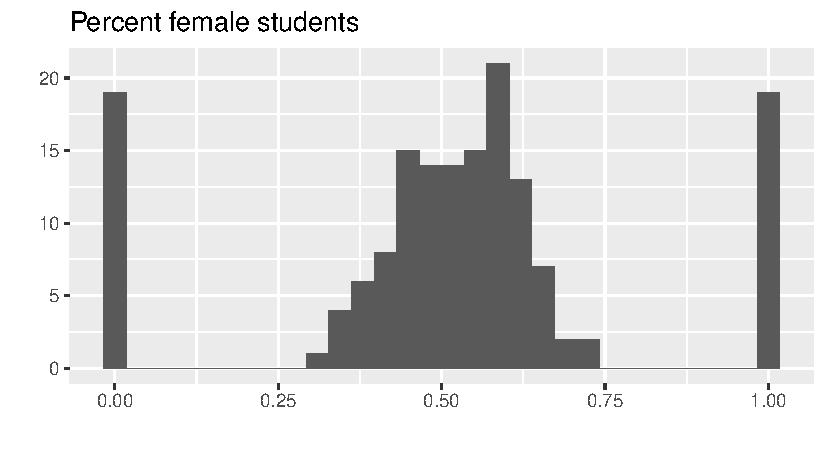
\includegraphics{summary_plots_files/figure-pdf/unnamed-chunk-13-1.pdf}

}

\end{figure}

Note the single sex (catholic) schools. We can facet to see both groups:

\begin{Shaded}
\begin{Highlighting}[]
\FunctionTok{qplot}\NormalTok{( per.fem, }\AttributeTok{data=}\NormalTok{aggdat,}
       \AttributeTok{main =} \StringTok{"Percent female students"}\NormalTok{, }
       \AttributeTok{xlab =} \StringTok{""}\NormalTok{) }\SpecialCharTok{+}
  \FunctionTok{facet\_wrap}\NormalTok{( }\SpecialCharTok{\textasciitilde{}}\NormalTok{ sector )}
\end{Highlighting}
\end{Shaded}

\begin{verbatim}
`stat_bin()` using `bins = 30`. Pick better value with `binwidth`.
\end{verbatim}

\begin{figure}[H]

{\centering \includegraphics{summary_plots_files/figure-pdf/unnamed-chunk-14-1.pdf}

}

\end{figure}

\hypertarget{diagnostic-plots}{%
\section{Diagnostic plots}\label{diagnostic-plots}}

We can also make some disagnostic plots for our model. first, let's fit
a random intercept model.

\begin{Shaded}
\begin{Highlighting}[]
\NormalTok{m1 }\OtherTok{\textless{}{-}} \FunctionTok{lmer}\NormalTok{(mathach }\SpecialCharTok{\textasciitilde{}} \DecValTok{1} \SpecialCharTok{+}\NormalTok{ ses }\SpecialCharTok{+}\NormalTok{ (}\DecValTok{1}\SpecialCharTok{|}\NormalTok{schoolid), }\AttributeTok{data=}\NormalTok{dat)}
\NormalTok{arm}\SpecialCharTok{::}\FunctionTok{display}\NormalTok{(m1)}
\end{Highlighting}
\end{Shaded}

\begin{verbatim}
lmer(formula = mathach ~ 1 + ses + (1 | schoolid), data = dat)
            coef.est coef.se
(Intercept) 12.66     0.19  
ses          2.39     0.11  

Error terms:
 Groups   Name        Std.Dev.
 schoolid (Intercept) 2.18    
 Residual             6.09    
---
number of obs: 7185, groups: schoolid, 160
AIC = 46653.2, DIC = 46637
deviance = 46641.0 
\end{verbatim}

We can check if some of our assumptions are being grossly violated,
i.e.~residuals at all levels are normally distributed.

\begin{Shaded}
\begin{Highlighting}[]
  \FunctionTok{qplot}\NormalTok{(}\FunctionTok{ranef}\NormalTok{(m1)}\SpecialCharTok{$}\NormalTok{schoolid[,}\DecValTok{1}\NormalTok{],}
       \AttributeTok{main =} \StringTok{"Histogram of random intercepts"}\NormalTok{, }\AttributeTok{xlab=}\StringTok{""}\NormalTok{)}
\end{Highlighting}
\end{Shaded}

\begin{verbatim}
`stat_bin()` using `bins = 30`. Pick better value with `binwidth`.
\end{verbatim}

\begin{figure}[H]

{\centering 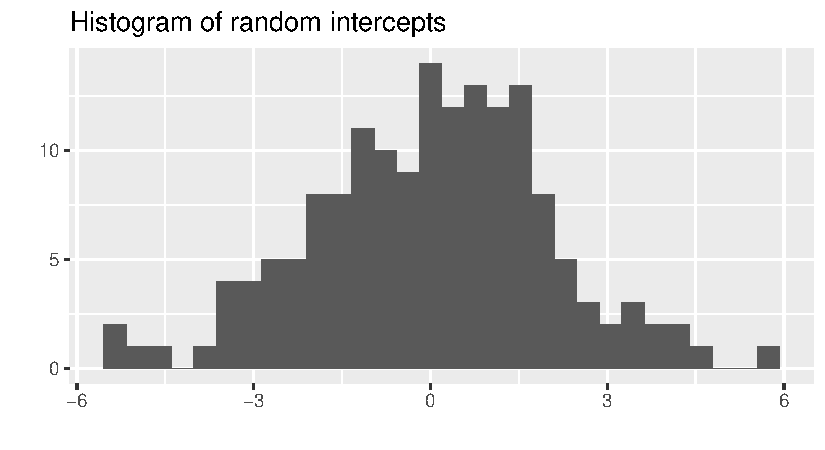
\includegraphics{summary_plots_files/figure-pdf/unnamed-chunk-16-1.pdf}

}

\end{figure}

\begin{Shaded}
\begin{Highlighting}[]
  \FunctionTok{qplot}\NormalTok{(}\FunctionTok{resid}\NormalTok{(m1), }
       \AttributeTok{main =} \StringTok{"Hisogram of residuals"}\NormalTok{)}
\end{Highlighting}
\end{Shaded}

\begin{verbatim}
`stat_bin()` using `bins = 30`. Pick better value with `binwidth`.
\end{verbatim}

\begin{figure}[H]

{\centering 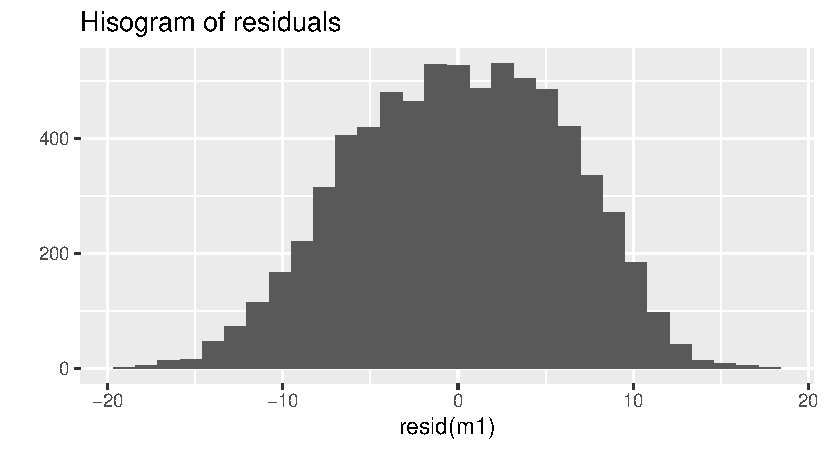
\includegraphics{summary_plots_files/figure-pdf/unnamed-chunk-16-2.pdf}

}

\end{figure}

We can check for heteroskedasticity by plotting residuals against
predicted values

\begin{Shaded}
\begin{Highlighting}[]
\NormalTok{  dat}\SpecialCharTok{$}\NormalTok{yhat  }\OtherTok{=} \FunctionTok{predict}\NormalTok{(m1)}
\NormalTok{  dat}\SpecialCharTok{$}\NormalTok{resid }\OtherTok{=} \FunctionTok{resid}\NormalTok{(m1)}
  
  \FunctionTok{ggplot}\NormalTok{(dat, }\FunctionTok{aes}\NormalTok{(yhat, resid)) }\SpecialCharTok{+} 
      \FunctionTok{geom\_point}\NormalTok{(}\AttributeTok{alpha=}\FloatTok{0.3}\NormalTok{) }\SpecialCharTok{+} 
      \FunctionTok{geom\_smooth}\NormalTok{() }\SpecialCharTok{+} 
      \FunctionTok{labs}\NormalTok{(}\AttributeTok{title =} \StringTok{"Residuals against predicted values"}\NormalTok{,}
           \AttributeTok{x =} \StringTok{"Predicted values"}\NormalTok{, }\AttributeTok{y =}\StringTok{"Residuals"}\NormalTok{)}
\end{Highlighting}
\end{Shaded}

\begin{verbatim}
`geom_smooth()` using method = 'gam' and formula = 'y ~ s(x, bs = "cs")'
\end{verbatim}

\begin{figure}[H]

{\centering 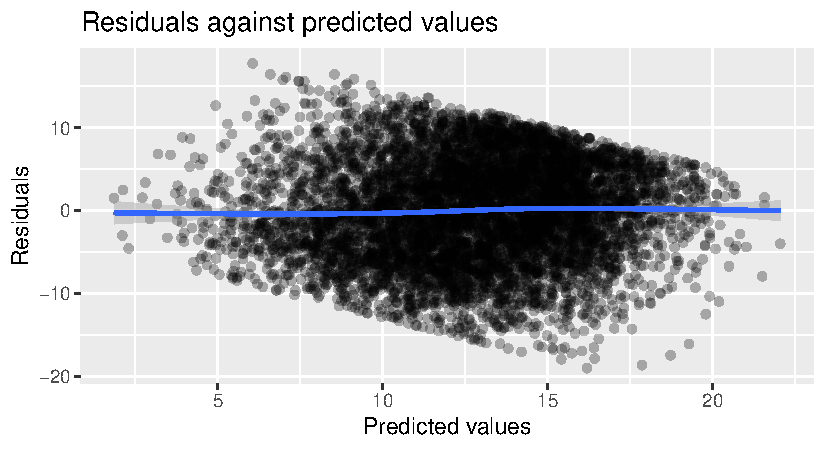
\includegraphics{summary_plots_files/figure-pdf/unnamed-chunk-17-1.pdf}

}

\end{figure}

It looks reasonable (up to the discrete and bounded nature of our data).
No major weird curves in the loess line through the residuals means
linearity is a reasonable assumption. That being said, our nominal SEs
around our loess line are tight, so the mild curve is probably evidence
of \emph{some} model misfit.

We can also look at the distribution of random effects using the
\texttt{lattice} package

\begin{Shaded}
\begin{Highlighting}[]
  \FunctionTok{library}\NormalTok{(lattice)}
  \FunctionTok{qqmath}\NormalTok{(}\FunctionTok{ranef}\NormalTok{(m1, }\AttributeTok{condVar=}\ConstantTok{TRUE}\NormalTok{), }\AttributeTok{strip=}\ConstantTok{FALSE}\NormalTok{)}
\end{Highlighting}
\end{Shaded}

\begin{verbatim}
$schoolid
\end{verbatim}

\begin{figure}[H]

{\centering 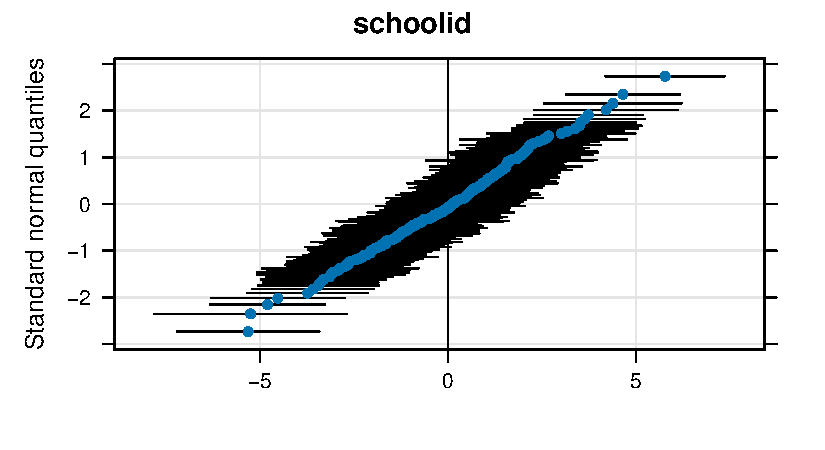
\includegraphics{summary_plots_files/figure-pdf/unnamed-chunk-18-1.pdf}

}

\end{figure}

\hypertarget{example-of-making-plots-with-expand.grid}{%
\chapter{\texorpdfstring{Example of making plots with
\texttt{expand.grid}}{Example of making plots with expand.grid}}\label{example-of-making-plots-with-expand.grid}}

\hypertarget{introduction-2}{%
\section{Introduction}\label{introduction-2}}

This script demonstrates using the \texttt{predict()} function to make
plots with separate lines for different groups. A core element is the
\texttt{expand.grid()} method. The central idea is this: for each of our
groups we manually create a series of points at different levels of our
covariate (e.g.~ses or time) and then predict the outcome for each of
these values. We then plot these predicted points, and it makes a smooth
curve for that group.

In this document we start with clustered data (the HS\&B dataset) and
then illustrate how to this with longitudinal data as well.

\hypertarget{making-plots-for-the-hsb-dataset}{%
\section{Making plots for the HS\&B
Dataset}\label{making-plots-for-the-hsb-dataset}}

In this section we first look at how to plot the model results by making
a tiny dataset from the fixed effects, and then we extend to more
powerful plotting of individual schools.

\hypertarget{setting-up-the-hsb-data}{%
\subsection{Setting up the HS\&B data}\label{setting-up-the-hsb-data}}

The ``many small worlds'' view says each school has its own regression
line. We are going to plot them all. See the lecture code files for how
to load the HS\&B dataset. For clarity it is omitted from the printout.
We end up with this for the schools:

\begin{Shaded}
\begin{Highlighting}[]
\FunctionTok{head}\NormalTok{( sdat )}
\end{Highlighting}
\end{Shaded}

\begin{verbatim}
    id size   sector meanses
1 1224  842   public  -0.428
2 1288 1855   public   0.128
3 1296 1719   public  -0.420
4 1308  716 catholic   0.534
5 1317  455 catholic   0.351
6 1358 1430   public  -0.014
\end{verbatim}

and this for students (we merged in the school info already):

\begin{Shaded}
\begin{Highlighting}[]
\FunctionTok{head}\NormalTok{( dat )}
\end{Highlighting}
\end{Shaded}

\begin{verbatim}
    id minority female    ses mathach size sector meanses
1 1224        0      1 -1.528   5.876  842 public  -0.428
2 1224        0      1 -0.588  19.708  842 public  -0.428
3 1224        0      0 -0.528  20.349  842 public  -0.428
4 1224        0      0 -0.668   8.781  842 public  -0.428
5 1224        0      0 -0.158  17.898  842 public  -0.428
6 1224        0      0  0.022   4.583  842 public  -0.428
\end{verbatim}

We fit a fancy random slopes model with 2nd level covariates that impact
both the overall school means and the ses by math achievment slopes. Our
model is \[
\begin{aligned}
y_{ij} &= \beta_{0j} + \beta_{1j} ses_{ij} +  \epsilon_{ij} \\
\beta_{0j} &= \gamma_{00} + \gamma_{01} sector_j + u_{0j} \\
\beta_{1j} &= \gamma_{10} + \gamma_{11} sector_j + u_{1j} 
\end{aligned}
\] We omit the equations for the random effect distributions. The
\(\epsilon_{ij}\) are normal, and the \((u_{0j},u_{1j})\) are bivariate
normal, as usual. We fit the model as so:

\begin{Shaded}
\begin{Highlighting}[]
\NormalTok{M1 }\OtherTok{=} \FunctionTok{lmer}\NormalTok{( mathach }\SpecialCharTok{\textasciitilde{}} \DecValTok{1} \SpecialCharTok{+}\NormalTok{ ses}\SpecialCharTok{*}\NormalTok{sector }\SpecialCharTok{+}\NormalTok{ (}\DecValTok{1} \SpecialCharTok{+}\NormalTok{ ses}\SpecialCharTok{|}\NormalTok{id), }\AttributeTok{data=}\NormalTok{dat )}
\end{Highlighting}
\end{Shaded}

\begin{verbatim}
Warning in checkConv(attr(opt, "derivs"), opt$par, ctrl = control$checkConv, :
Model failed to converge with max|grad| = 0.00578929 (tol = 0.002, component 1)
\end{verbatim}

\begin{Shaded}
\begin{Highlighting}[]
\FunctionTok{display}\NormalTok{( M1 )}
\end{Highlighting}
\end{Shaded}

\begin{verbatim}
lmer(formula = mathach ~ 1 + ses * sector + (1 + ses | id), data = dat)
                   coef.est coef.se
(Intercept)        11.75     0.23  
ses                 2.96     0.14  
sectorcatholic      2.13     0.35  
ses:sectorcatholic -1.31     0.22  

Error terms:
 Groups   Name        Std.Dev. Corr 
 id       (Intercept) 1.95          
          ses         0.28     1.00 
 Residual             6.07          
---
number of obs: 7185, groups: id, 160
AIC = 46585.1, DIC = 46557.2
deviance = 46563.2 
\end{verbatim}

\hypertarget{plotting-the-model-results}{%
\subsection{Plotting the model
results}\label{plotting-the-model-results}}

We can plot the model results by making a little dataset by hand. This
section of the handout illustrates how you can hand-construct plots by
directly calculating predicted values from your model. This is a very
useful skill, and we recommend studying this area of the handout as a
way of learning how to control plotting at a very direct level.

So, to continue, we proceed in three steps.

\emph{Step 1: Decide on the plot.} Let's make a plot of outcome vs.~ses
with two lines (one for catholic and one for public). Sometimes it is
worth actually sketching the desired plot on scratch paper, identifying
the x and y axes and general lines desired.

\emph{Step 2: calculate some outcomes using our model.} We do this by
deciding what values we want to plot, and then making the outcome.

\begin{Shaded}
\begin{Highlighting}[]
\FunctionTok{quantile}\NormalTok{( dat}\SpecialCharTok{$}\NormalTok{ses, }\FunctionTok{c}\NormalTok{( }\FloatTok{0.05}\NormalTok{, }\FloatTok{0.95}\NormalTok{ ) )}
\end{Highlighting}
\end{Shaded}

\begin{verbatim}
    5%    95% 
-1.318  1.212 
\end{verbatim}

\begin{Shaded}
\begin{Highlighting}[]
\NormalTok{plt }\OtherTok{=} \FunctionTok{data.frame}\NormalTok{( }\AttributeTok{ses =} \FunctionTok{c}\NormalTok{(}\SpecialCharTok{{-}}\FloatTok{1.5}\NormalTok{, }\FloatTok{1.25}\NormalTok{, }\SpecialCharTok{{-}}\FloatTok{1.5}\NormalTok{, }\FloatTok{1.25}\NormalTok{ ),}
                  \AttributeTok{catholic =} \FunctionTok{c}\NormalTok{( }\DecValTok{0}\NormalTok{, }\DecValTok{0}\NormalTok{, }\DecValTok{1}\NormalTok{, }\DecValTok{1}\NormalTok{ ) )}
\NormalTok{cf }\OtherTok{=} \FunctionTok{fixef}\NormalTok{( M1 )}
\NormalTok{cf}
\end{Highlighting}
\end{Shaded}

\begin{verbatim}
       (Intercept)                ses     sectorcatholic ses:sectorcatholic 
         11.751789           2.957538           2.129531          -1.313363 
\end{verbatim}

\begin{Shaded}
\begin{Highlighting}[]
\NormalTok{plt }\OtherTok{=} \FunctionTok{mutate}\NormalTok{( plt,}
              \AttributeTok{Y =}\NormalTok{ cf[[}\DecValTok{1}\NormalTok{]] }\SpecialCharTok{+}\NormalTok{ cf[[}\DecValTok{2}\NormalTok{]]}\SpecialCharTok{*}\NormalTok{ses }\SpecialCharTok{+}\NormalTok{ cf[[}\DecValTok{3}\NormalTok{]]}\SpecialCharTok{*}\NormalTok{catholic }\SpecialCharTok{+}\NormalTok{ cf[[}\DecValTok{4}\NormalTok{]]}\SpecialCharTok{*}\NormalTok{ses}\SpecialCharTok{*}\NormalTok{catholic )}
\NormalTok{plt}
\end{Highlighting}
\end{Shaded}

\begin{verbatim}
    ses catholic         Y
1 -1.50        0  7.315482
2  1.25        0 15.448711
3 -1.50        1 11.415057
4  1.25        1 15.936538
\end{verbatim}

Note that we have made a little mini-dataset with just the points we
want to put on our plot. We calculated these points ``by hand''. There
is no shame in this.

\emph{Step 3: plot.} We plot using ggplot:

\begin{Shaded}
\begin{Highlighting}[]
\NormalTok{plt}\SpecialCharTok{$}\NormalTok{catholic }\OtherTok{=} \FunctionTok{factor}\NormalTok{( plt}\SpecialCharTok{$}\NormalTok{catholic, }
                       \AttributeTok{labels=}\FunctionTok{c}\NormalTok{(}\StringTok{"public"}\NormalTok{,}\StringTok{"catholic"}\NormalTok{),}
                       \AttributeTok{levels=}\FunctionTok{c}\NormalTok{(}\DecValTok{0}\NormalTok{,}\DecValTok{1}\NormalTok{) )}
\FunctionTok{ggplot}\NormalTok{( plt, }\FunctionTok{aes}\NormalTok{( ses, Y, }\AttributeTok{col=}\NormalTok{catholic ) ) }\SpecialCharTok{+}
    \FunctionTok{geom\_line}\NormalTok{()}
\end{Highlighting}
\end{Shaded}

\begin{figure}[H]

{\centering \includegraphics{plot_expand_grid_files/figure-pdf/unnamed-chunk-6-1.pdf}

}

\end{figure}

\hypertarget{a-fancy-diversion-categorical-variables-on-the-x-axis}{%
\subsubsection{\texorpdfstring{A fancy diversion: categorical variables
on the
\(x\)-axis}{A fancy diversion: categorical variables on the x-axis}}\label{a-fancy-diversion-categorical-variables-on-the-x-axis}}

Say we decided to fit a model where we have ses \textbf{categories}:

\begin{Shaded}
\begin{Highlighting}[]
\NormalTok{dat}\SpecialCharTok{$}\NormalTok{ses.cat }\OtherTok{=} \FunctionTok{cut}\NormalTok{( dat}\SpecialCharTok{$}\NormalTok{ses, }
                   \AttributeTok{breaks=}\FunctionTok{quantile}\NormalTok{( dat}\SpecialCharTok{$}\NormalTok{ses, }\FunctionTok{c}\NormalTok{( }\DecValTok{0}\NormalTok{, }\FloatTok{0.33}\NormalTok{, }\FloatTok{0.67}\NormalTok{, }\DecValTok{1}\NormalTok{ ) ),}
                   \AttributeTok{labels =} \FunctionTok{c}\NormalTok{( }\StringTok{"low"}\NormalTok{,}\StringTok{"mid"}\NormalTok{,}\StringTok{"high"}\NormalTok{),}
                   \AttributeTok{include.lowest =} \ConstantTok{TRUE}\NormalTok{ )}
\FunctionTok{table}\NormalTok{( dat}\SpecialCharTok{$}\NormalTok{ses.cat )}
\end{Highlighting}
\end{Shaded}

\begin{verbatim}

 low  mid high 
2371 2462 2352 
\end{verbatim}

\begin{Shaded}
\begin{Highlighting}[]
\NormalTok{M1b }\OtherTok{=} \FunctionTok{lmer}\NormalTok{( mathach }\SpecialCharTok{\textasciitilde{}} \DecValTok{1} \SpecialCharTok{+}\NormalTok{ ses.cat}\SpecialCharTok{*}\NormalTok{sector }\SpecialCharTok{+}\NormalTok{ (}\DecValTok{1} \SpecialCharTok{+}\NormalTok{ ses}\SpecialCharTok{|}\NormalTok{id), }\AttributeTok{data=}\NormalTok{dat )}
\FunctionTok{display}\NormalTok{( M1b )}
\end{Highlighting}
\end{Shaded}

\begin{verbatim}
lmer(formula = mathach ~ 1 + ses.cat * sector + (1 + ses | id), 
    data = dat)
                           coef.est coef.se
(Intercept)                 9.19     0.27  
ses.catmid                  2.28     0.25  
ses.cathigh                 5.07     0.29  
sectorcatholic              3.44     0.42  
ses.catmid:sectorcatholic  -0.98     0.38  
ses.cathigh:sectorcatholic -2.47     0.42  

Error terms:
 Groups   Name        Std.Dev. Corr 
 id       (Intercept) 2.05          
          ses         0.47     0.23 
 Residual             6.10          
---
number of obs: 7185, groups: id, 160
AIC = 46691.5, DIC = 46660.7
deviance = 46666.1 
\end{verbatim}

Make our outcomes:

\begin{Shaded}
\begin{Highlighting}[]
\NormalTok{plt }\OtherTok{=} \FunctionTok{data.frame}\NormalTok{( }\AttributeTok{ses.mid =} \FunctionTok{c}\NormalTok{( }\DecValTok{0}\NormalTok{, }\DecValTok{1}\NormalTok{, }\DecValTok{0}\NormalTok{, }\DecValTok{0}\NormalTok{, }\DecValTok{1}\NormalTok{, }\DecValTok{0}\NormalTok{ ),}
                  \AttributeTok{ses.high =} \FunctionTok{c}\NormalTok{( }\DecValTok{0}\NormalTok{, }\DecValTok{0}\NormalTok{, }\DecValTok{1}\NormalTok{, }\DecValTok{0}\NormalTok{, }\DecValTok{0}\NormalTok{, }\DecValTok{1}\NormalTok{ ),}
                  \AttributeTok{catholic =} \FunctionTok{c}\NormalTok{( }\DecValTok{0}\NormalTok{, }\DecValTok{0}\NormalTok{, }\DecValTok{0}\NormalTok{, }\DecValTok{1}\NormalTok{, }\DecValTok{1}\NormalTok{, }\DecValTok{1}\NormalTok{ ) )}
\NormalTok{cf }\OtherTok{=} \FunctionTok{fixef}\NormalTok{( M1b )}
\NormalTok{cf}
\end{Highlighting}
\end{Shaded}

\begin{verbatim}
               (Intercept)                 ses.catmid 
                 9.1915044                  2.2808807 
               ses.cathigh             sectorcatholic 
                 5.0721921                  3.4398984 
 ses.catmid:sectorcatholic ses.cathigh:sectorcatholic 
                -0.9759927                 -2.4707460 
\end{verbatim}

\begin{Shaded}
\begin{Highlighting}[]
\NormalTok{plt }\OtherTok{=} \FunctionTok{mutate}\NormalTok{( plt,}
              \AttributeTok{Y =}\NormalTok{ cf[[}\DecValTok{1}\NormalTok{]] }\SpecialCharTok{+}\NormalTok{ cf[[}\DecValTok{2}\NormalTok{]]}\SpecialCharTok{*}\NormalTok{ses.mid }\SpecialCharTok{+}\NormalTok{ cf[[}\DecValTok{3}\NormalTok{]]}\SpecialCharTok{*}\NormalTok{ses.high }\SpecialCharTok{+}
\NormalTok{                cf[[}\DecValTok{4}\NormalTok{]]}\SpecialCharTok{*}\NormalTok{catholic }\SpecialCharTok{+}\NormalTok{ cf[[}\DecValTok{5}\NormalTok{]]}\SpecialCharTok{*}\NormalTok{ses.mid}\SpecialCharTok{*}\NormalTok{catholic }\SpecialCharTok{+}\NormalTok{ cf[[}\DecValTok{6}\NormalTok{]]}\SpecialCharTok{*}\NormalTok{ses.high}\SpecialCharTok{*}\NormalTok{catholic )}
\NormalTok{plt}
\end{Highlighting}
\end{Shaded}

\begin{verbatim}
  ses.mid ses.high catholic         Y
1       0        0        0  9.191504
2       1        0        0 11.472385
3       0        1        0 14.263697
4       0        0        1 12.631403
5       1        0        1 13.936291
6       0        1        1 15.232849
\end{verbatim}

And plot

\begin{Shaded}
\begin{Highlighting}[]
\NormalTok{plt}\SpecialCharTok{$}\NormalTok{catholic }\OtherTok{=} \FunctionTok{factor}\NormalTok{( plt}\SpecialCharTok{$}\NormalTok{catholic, }
                       \AttributeTok{labels=}\FunctionTok{c}\NormalTok{(}\StringTok{"public"}\NormalTok{,}\StringTok{"catholic"}\NormalTok{),}
                       \AttributeTok{levels=}\FunctionTok{c}\NormalTok{(}\DecValTok{0}\NormalTok{,}\DecValTok{1}\NormalTok{) )}
\NormalTok{plt}\SpecialCharTok{$}\NormalTok{ses }\OtherTok{=} \StringTok{"low"}
\NormalTok{plt}\SpecialCharTok{$}\NormalTok{ses[plt}\SpecialCharTok{$}\NormalTok{ses.mid}\SpecialCharTok{==}\DecValTok{1}\NormalTok{] }\OtherTok{=} \StringTok{"mid"}
\NormalTok{plt}\SpecialCharTok{$}\NormalTok{ses[plt}\SpecialCharTok{$}\NormalTok{ses.high}\SpecialCharTok{==}\DecValTok{1}\NormalTok{] }\OtherTok{=} \StringTok{"high"}
\NormalTok{plt}\SpecialCharTok{$}\NormalTok{ses }\OtherTok{=} \FunctionTok{factor}\NormalTok{( plt}\SpecialCharTok{$}\NormalTok{ses, }\AttributeTok{levels=}\FunctionTok{c}\NormalTok{(}\StringTok{"low"}\NormalTok{,}\StringTok{"mid"}\NormalTok{,}\StringTok{"high"}\NormalTok{) )}
\FunctionTok{ggplot}\NormalTok{( plt, }\FunctionTok{aes}\NormalTok{( ses, Y, }\AttributeTok{col=}\NormalTok{catholic, }\AttributeTok{group=}\NormalTok{catholic ) ) }\SpecialCharTok{+}
    \FunctionTok{geom\_line}\NormalTok{() }\SpecialCharTok{+} \FunctionTok{geom\_point}\NormalTok{()}
\end{Highlighting}
\end{Shaded}

\begin{figure}[H]

{\centering \includegraphics{plot_expand_grid_files/figure-pdf/unnamed-chunk-9-1.pdf}

}

\end{figure}

Note the \emph{very important} \texttt{group=catholic} line that tells
the plot to group everyone by catholic. If not, it will get confused and
note that since ses is categorical, try to group on that. Then it cannot
make a line since each group has only a single point.

\hypertarget{plotting-individual-school-regression-lines}{%
\subsection{Plotting individual school regression
lines}\label{plotting-individual-school-regression-lines}}

We can plot the individual lines by hand-calculating the school level
slopes and intercepts. This code shows how:

\begin{Shaded}
\begin{Highlighting}[]
\NormalTok{coefs }\OtherTok{=} \FunctionTok{coef}\NormalTok{( M1 )}\SpecialCharTok{$}\NormalTok{id}
\FunctionTok{head}\NormalTok{( coefs )}
\end{Highlighting}
\end{Shaded}

\begin{verbatim}
     (Intercept)      ses sectorcatholic ses:sectorcatholic
1224   11.084408 2.863501       2.129531          -1.313363
1288   12.761032 3.099743       2.129531          -1.313363
1296    9.193415 2.597052       2.129531          -1.313363
1308   12.709882 3.092535       2.129531          -1.313363
1317   10.719013 2.812016       2.129531          -1.313363
1358   11.478455 2.919031       2.129531          -1.313363
\end{verbatim}

\begin{Shaded}
\begin{Highlighting}[]
\NormalTok{coefs }\OtherTok{=} \FunctionTok{rename}\NormalTok{( coefs, }
                \AttributeTok{gamma.00 =} \StringTok{\textasciigrave{}}\AttributeTok{(Intercept)}\StringTok{\textasciigrave{}}\NormalTok{,}
                \AttributeTok{gamma.10 =} \StringTok{\textasciigrave{}}\AttributeTok{ses}\StringTok{\textasciigrave{}}\NormalTok{,}
                \AttributeTok{gamma.01 =} \StringTok{\textasciigrave{}}\AttributeTok{sectorcatholic}\StringTok{\textasciigrave{}}\NormalTok{,}
                \AttributeTok{gamma.11 =} \StringTok{\textasciigrave{}}\AttributeTok{ses:sectorcatholic}\StringTok{\textasciigrave{}}\NormalTok{ )}
\NormalTok{coefs}\SpecialCharTok{$}\NormalTok{id }\OtherTok{=} \FunctionTok{rownames}\NormalTok{( coefs )}
\NormalTok{coefs }\OtherTok{=} \FunctionTok{merge}\NormalTok{( coefs, sdat, }\AttributeTok{by=}\StringTok{"id"}\NormalTok{ )}
\NormalTok{coefs }\OtherTok{=} \FunctionTok{mutate}\NormalTok{( coefs,}
                \AttributeTok{beta.0 =}\NormalTok{ gamma}\FloatTok{.00} \SpecialCharTok{+}\NormalTok{ gamma}\FloatTok{.01} \SpecialCharTok{*}\NormalTok{ (sector}\SpecialCharTok{==}\StringTok{"catholic"}\NormalTok{),}
                \AttributeTok{beta.1 =}\NormalTok{ gamma}\FloatTok{.10} \SpecialCharTok{+}\NormalTok{ gamma}\FloatTok{.11} \SpecialCharTok{*}\NormalTok{ (sector}\SpecialCharTok{==}\StringTok{"catholic"}\NormalTok{) )}
\end{Highlighting}
\end{Shaded}

Note how we have to add up our gammas to get our betas for each school.
See our final betas, one set for each school:

\begin{Shaded}
\begin{Highlighting}[]
\FunctionTok{head}\NormalTok{( dplyr}\SpecialCharTok{::}\FunctionTok{select}\NormalTok{( coefs, }\SpecialCharTok{{-}}\NormalTok{gamma}\FloatTok{.00}\NormalTok{, }\SpecialCharTok{{-}}\NormalTok{gamma}\FloatTok{.10}\NormalTok{, }\SpecialCharTok{{-}}\NormalTok{gamma}\FloatTok{.01}\NormalTok{, }\SpecialCharTok{{-}}\NormalTok{gamma}\FloatTok{.11}\NormalTok{ ) )}
\end{Highlighting}
\end{Shaded}

\begin{verbatim}
    id size   sector meanses    beta.0   beta.1
1 1224  842   public  -0.428 11.084408 2.863501
2 1288 1855   public   0.128 12.761032 3.099743
3 1296 1719   public  -0.420  9.193415 2.597052
4 1308  716 catholic   0.534 14.839413 1.779172
5 1317  455 catholic   0.351 12.848543 1.498653
6 1358 1430   public  -0.014 11.478455 2.919031
\end{verbatim}

Now let's plot a subsample of 20 schools

\begin{Shaded}
\begin{Highlighting}[]
\FunctionTok{set.seed}\NormalTok{( }\DecValTok{102030}\NormalTok{ )}
\NormalTok{sub20 }\OtherTok{=} \FunctionTok{sample}\NormalTok{( }\FunctionTok{unique}\NormalTok{( dat}\SpecialCharTok{$}\NormalTok{id ), }\DecValTok{20}\NormalTok{ )}

\NormalTok{coefs}\FloatTok{.20} \OtherTok{=} \FunctionTok{filter}\NormalTok{( coefs, id }\SpecialCharTok{\%in\%}\NormalTok{ sub20 )}

\FunctionTok{ggplot}\NormalTok{( coefs}\FloatTok{.20}\NormalTok{, }\FunctionTok{aes}\NormalTok{( }\AttributeTok{group=}\NormalTok{id ) ) }\SpecialCharTok{+}
  \FunctionTok{geom\_abline}\NormalTok{( }\FunctionTok{aes}\NormalTok{( }\AttributeTok{slope=}\NormalTok{beta}\FloatTok{.1}\NormalTok{, }\AttributeTok{intercept=}\NormalTok{beta}\FloatTok{.0}\NormalTok{, }\AttributeTok{col=}\NormalTok{sector) ) }\SpecialCharTok{+}
  \FunctionTok{coord\_cartesian}\NormalTok{( }\AttributeTok{xlim=}\FunctionTok{c}\NormalTok{(}\SpecialCharTok{{-}}\FloatTok{2.5}\NormalTok{,}\DecValTok{2}\NormalTok{), }\AttributeTok{ylim=}\FunctionTok{range}\NormalTok{(dat}\SpecialCharTok{$}\NormalTok{mathach) )}
\end{Highlighting}
\end{Shaded}

\begin{figure}[H]

{\centering 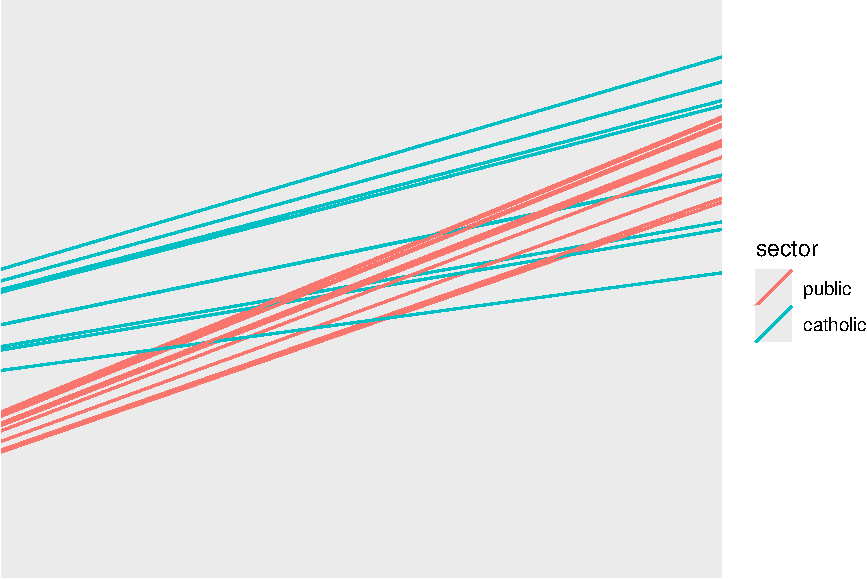
\includegraphics{plot_expand_grid_files/figure-pdf/unnamed-chunk-12-1.pdf}

}

\end{figure}

\emph{Commentary:} We need to specify the size of the plot since we have
no data, just the intercepts and slopes. We are using the Emperical
Bayes estimates of the random effects added to our school level fixed
effects to get the \(\hat{\beta}_{0j}, \hat{\beta}_{1j}\) which define
the school-specific regression line for school \(j\).

Our two types of school are clearly separated. Catholic schools have
higher average performance, and less of a ses-achievement relationship.
Since we have merged in our school level data, we can color the lines by
catholic vs public, making our plot easier to read.

\hypertarget{plotting-with-predict}{%
\subsection{Plotting with predict()}\label{plotting-with-predict}}

A more general plotitng approach is to plot using \texttt{predict()},
where for each student we predict the outcome.

\begin{Shaded}
\begin{Highlighting}[]
\NormalTok{dat}\SpecialCharTok{$}\NormalTok{math.hat }\OtherTok{=} \FunctionTok{predict}\NormalTok{( M1 )}
\end{Highlighting}
\end{Shaded}

Now let's plot a subsample of 20 schools

\begin{Shaded}
\begin{Highlighting}[]
\NormalTok{dat}\FloatTok{.20} \OtherTok{=} \FunctionTok{filter}\NormalTok{( dat, id }\SpecialCharTok{\%in\%}\NormalTok{ sub20 )}

\FunctionTok{ggplot}\NormalTok{( dat}\FloatTok{.20}\NormalTok{, }\FunctionTok{aes}\NormalTok{( ses, math.hat, }\AttributeTok{group=}\NormalTok{id, }\AttributeTok{col=}\NormalTok{sector ) ) }\SpecialCharTok{+}
  \FunctionTok{geom\_line}\NormalTok{()}
\end{Highlighting}
\end{Shaded}

\begin{figure}[H]

{\centering \includegraphics{plot_expand_grid_files/figure-pdf/unnamed-chunk-14-1.pdf}

}

\end{figure}

But look at how the lines don't go the full distance. What ggplot is
doing is plotting the individual students, and connecting them with a
line. We can see this by plotting the students as well, like this:

\begin{Shaded}
\begin{Highlighting}[]
\FunctionTok{ggplot}\NormalTok{( dat}\FloatTok{.20}\NormalTok{, }\FunctionTok{aes}\NormalTok{( ses, math.hat, }\AttributeTok{group=}\NormalTok{id, }\AttributeTok{col=}\NormalTok{sector ) ) }\SpecialCharTok{+}
  \FunctionTok{geom\_line}\NormalTok{() }\SpecialCharTok{+}
  \FunctionTok{geom\_point}\NormalTok{()}
\end{Highlighting}
\end{Shaded}

\begin{figure}[H]

{\centering 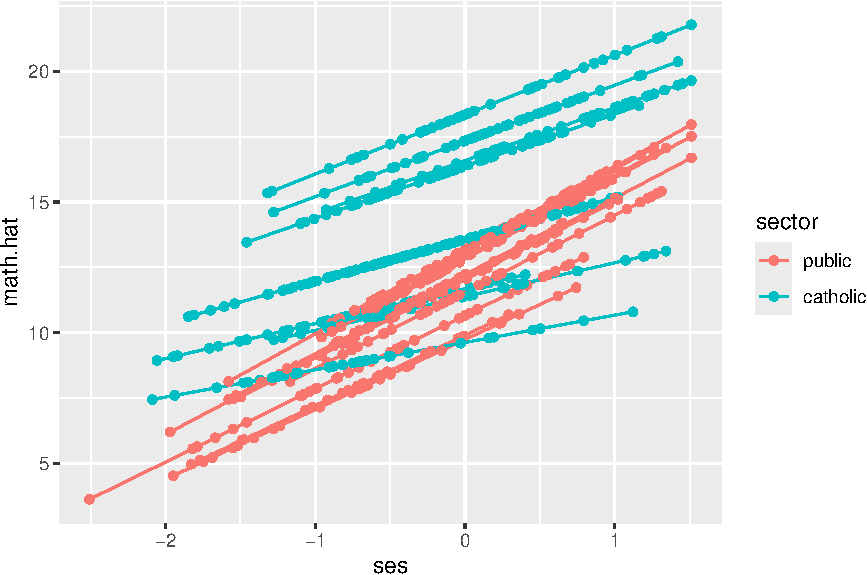
\includegraphics{plot_expand_grid_files/figure-pdf/unnamed-chunk-15-1.pdf}

}

\end{figure}

We have a predicted outcome for each student, which removes the student
residual, giving just the school trends. If we don't have students for
some range of ses for a school, we won't have points in our plot for
that range for that school. The lines thus give the ranges (left to
right) of the ses values in each school.

\hypertarget{making-our-lines-go-the-same-length-with-expand.grid}{%
\subsection{Making our lines go the same length with
expand.grid()}\label{making-our-lines-go-the-same-length-with-expand.grid}}

The way we fix this is we, for each school, make a bunch of fake
students with different SES and predict along all those fake students.
This will give us equally spaced lines.

That being said: the shorter lines above are also informative, as they
give you a sense of what the range of ses for each school actually is.
Which approach is somewhat a matter of taste.

We can generate fake children of each group for each school using
\texttt{expand.grid()}. This method will generate a dataframe with all
combinations of the given variables supplied. Here we make all
combinations of ses, for a set of ses values, and school id.

\begin{Shaded}
\begin{Highlighting}[]
\NormalTok{synth.dat }\OtherTok{=} \FunctionTok{expand\_grid}\NormalTok{( }\AttributeTok{id =} \FunctionTok{unique}\NormalTok{( dat}\SpecialCharTok{$}\NormalTok{id ),}
                         \AttributeTok{ses =} \FunctionTok{seq}\NormalTok{( }\SpecialCharTok{{-}}\FloatTok{2.5}\NormalTok{, }\DecValTok{2}\NormalTok{, }\AttributeTok{length.out=}\DecValTok{9}\NormalTok{ ) )}
\FunctionTok{head}\NormalTok{( synth.dat )}
\end{Highlighting}
\end{Shaded}

\begin{verbatim}
# A tibble: 6 x 2
  id       ses
  <chr>  <dbl>
1 1224  -2.5  
2 1224  -1.94 
3 1224  -1.38 
4 1224  -0.812
5 1224  -0.25 
6 1224   0.312
\end{verbatim}

The \texttt{seq()} command makes an evenly spaced \emph{seq}uence of
numbers going from the first to the last, with 9 numbers. E.g.,

\begin{Shaded}
\begin{Highlighting}[]
\FunctionTok{seq}\NormalTok{( }\DecValTok{1}\NormalTok{, }\DecValTok{10}\NormalTok{, }\AttributeTok{length.out=}\DecValTok{4}\NormalTok{ )}
\end{Highlighting}
\end{Shaded}

\begin{verbatim}
[1]  1  4  7 10
\end{verbatim}

We then merge our school info back in to get sector for each school id:

\begin{Shaded}
\begin{Highlighting}[]
\NormalTok{synth.dat }\OtherTok{=} \FunctionTok{merge}\NormalTok{( synth.dat, sdat, }\AttributeTok{by=}\StringTok{"id"}\NormalTok{, }\AttributeTok{all.x=}\ConstantTok{TRUE}\NormalTok{ )}
\end{Highlighting}
\end{Shaded}

We finally predict for each school, predicting outcome for our fake kids
in each school.

\begin{Shaded}
\begin{Highlighting}[]
\NormalTok{synth.dat}\SpecialCharTok{$}\NormalTok{math.hat }\OtherTok{=} \FunctionTok{predict}\NormalTok{( M1, }\AttributeTok{newdata=}\NormalTok{synth.dat )}
\end{Highlighting}
\end{Shaded}

We have predictions just as above, just for students that we set for
each school. The school random effects and everything remain because we
are using the original school ids.

Using our new data, plot 20 random schools--this code is the same as in
the prior subsection.

\begin{Shaded}
\begin{Highlighting}[]
\NormalTok{synth.dat}\FloatTok{.20} \OtherTok{=} \FunctionTok{filter}\NormalTok{( synth.dat, id }\SpecialCharTok{\%in\%}\NormalTok{ sub20 )}

\FunctionTok{ggplot}\NormalTok{( synth.dat}\FloatTok{.20}\NormalTok{, }\FunctionTok{aes}\NormalTok{( ses, math.hat, }\AttributeTok{group=}\NormalTok{id, }\AttributeTok{col=}\NormalTok{sector ) ) }\SpecialCharTok{+}
  \FunctionTok{geom\_line}\NormalTok{()}
\end{Highlighting}
\end{Shaded}

\begin{figure}[H]

{\centering 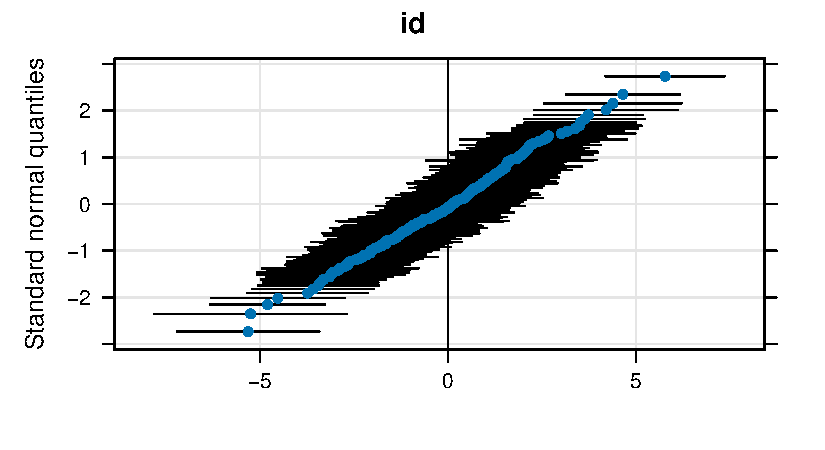
\includegraphics{plot_expand_grid_files/figure-pdf/unnamed-chunk-20-1.pdf}

}

\end{figure}

But see our equally spaced students?

\begin{Shaded}
\begin{Highlighting}[]
\FunctionTok{ggplot}\NormalTok{( synth.dat}\FloatTok{.20}\NormalTok{, }\FunctionTok{aes}\NormalTok{( ses, math.hat, }\AttributeTok{group=}\NormalTok{id, }\AttributeTok{col=}\NormalTok{sector ) ) }\SpecialCharTok{+}
  \FunctionTok{geom\_line}\NormalTok{() }\SpecialCharTok{+}
  \FunctionTok{geom\_point}\NormalTok{()}
\end{Highlighting}
\end{Shaded}

\begin{figure}[H]

{\centering \includegraphics{plot_expand_grid_files/figure-pdf/unnamed-chunk-21-1.pdf}

}

\end{figure}

\textbf{Why do this?} The \texttt{predict()} approach allows us to avoid
working with the gammas and adding them up like we did above. This is a
flexible and powerful approach that avoids a lot of work in many cases.
In the next section we illustrate by fitting curves rather than lines.
This would be very hard to do directly.

\hypertarget{superfancy-extra-bonus-plotting-of-complex-models}{%
\subsection{Superfancy extra bonus plotting of complex
models!}\label{superfancy-extra-bonus-plotting-of-complex-models}}

We can use predict for weird nonlinear relationships also. This will be
important for longitudinal data. To illustrate we fit a model that
allows a quadradic relationship between ses and math achievement.

\begin{Shaded}
\begin{Highlighting}[]
\NormalTok{dat}\SpecialCharTok{$}\NormalTok{ses2 }\OtherTok{=}\NormalTok{ dat}\SpecialCharTok{$}\NormalTok{ses}\SpecialCharTok{\^{}}\DecValTok{2}
\NormalTok{M2 }\OtherTok{=} \FunctionTok{lmer}\NormalTok{( mathach }\SpecialCharTok{\textasciitilde{}} \DecValTok{1} \SpecialCharTok{+}\NormalTok{ (ses }\SpecialCharTok{+}\NormalTok{ ses2)}\SpecialCharTok{*}\NormalTok{sector }\SpecialCharTok{+}\NormalTok{ meanses }\SpecialCharTok{+}\NormalTok{ (}\DecValTok{1} \SpecialCharTok{+}\NormalTok{ ses}\SpecialCharTok{|}\NormalTok{id), }\AttributeTok{data=}\NormalTok{dat )}

\FunctionTok{display}\NormalTok{( M2 )}
\end{Highlighting}
\end{Shaded}

\begin{verbatim}
lmer(formula = mathach ~ 1 + (ses + ses2) * sector + meanses + 
    (1 + ses | id), data = dat)
                    coef.est coef.se
(Intercept)         12.17     0.21  
ses                  2.79     0.15  
ses2                 0.04     0.13  
sectorcatholic       1.23     0.33  
meanses              3.14     0.38  
ses:sectorcatholic  -1.35     0.22  
ses2:sectorcatholic  0.06     0.21  

Error terms:
 Groups   Name        Std.Dev. Corr 
 id       (Intercept) 1.53          
          ses         0.23     0.49 
 Residual             6.07          
---
number of obs: 7185, groups: id, 160
AIC = 46539.7, DIC = 46495.9
deviance = 46506.8 
\end{verbatim}

To fit a quadratic model we need our quadratic ses term, which we make
by hand. We could also have used \texttt{I(ses\^{}2)} in the
\texttt{lmer()} command directly, but people don't tend to find that
easy to read.

And here we predict and plot:

\begin{Shaded}
\begin{Highlighting}[]
\NormalTok{synth.dat }\OtherTok{=} \FunctionTok{expand.grid}\NormalTok{( }\AttributeTok{id =} \FunctionTok{unique}\NormalTok{( dat}\SpecialCharTok{$}\NormalTok{id ),}
                         \AttributeTok{ses=} \FunctionTok{seq}\NormalTok{( }\SpecialCharTok{{-}}\FloatTok{2.5}\NormalTok{, }\DecValTok{2}\NormalTok{, }\AttributeTok{length.out=}\DecValTok{9}\NormalTok{ ) )}
\NormalTok{synth.dat}\SpecialCharTok{$}\NormalTok{ses2 }\OtherTok{=}\NormalTok{ synth.dat}\SpecialCharTok{$}\NormalTok{ses}\SpecialCharTok{\^{}}\DecValTok{2}
\NormalTok{synth.dat }\OtherTok{=} \FunctionTok{merge}\NormalTok{( synth.dat, sdat, }\AttributeTok{by=}\StringTok{"id"}\NormalTok{, }\AttributeTok{all.x=}\ConstantTok{TRUE}\NormalTok{ )}
\end{Highlighting}
\end{Shaded}

Note how we make our \texttt{ses2} variable out of \texttt{ses} just
like we did above.

\begin{Shaded}
\begin{Highlighting}[]
\NormalTok{synth.dat}\SpecialCharTok{$}\NormalTok{math.hat }\OtherTok{=} \FunctionTok{predict}\NormalTok{( M2, }\AttributeTok{newdata=}\NormalTok{synth.dat )}

\NormalTok{synth.dat}\FloatTok{.20} \OtherTok{=} \FunctionTok{filter}\NormalTok{( synth.dat, id }\SpecialCharTok{\%in\%}\NormalTok{ sub20 )}

\FunctionTok{ggplot}\NormalTok{( synth.dat}\FloatTok{.20}\NormalTok{, }\FunctionTok{aes}\NormalTok{( ses, math.hat, }\AttributeTok{group=}\NormalTok{id, }\AttributeTok{col=}\NormalTok{sector ) ) }\SpecialCharTok{+}
  \FunctionTok{geom\_line}\NormalTok{()}
\end{Highlighting}
\end{Shaded}

\begin{figure}[H]

{\centering 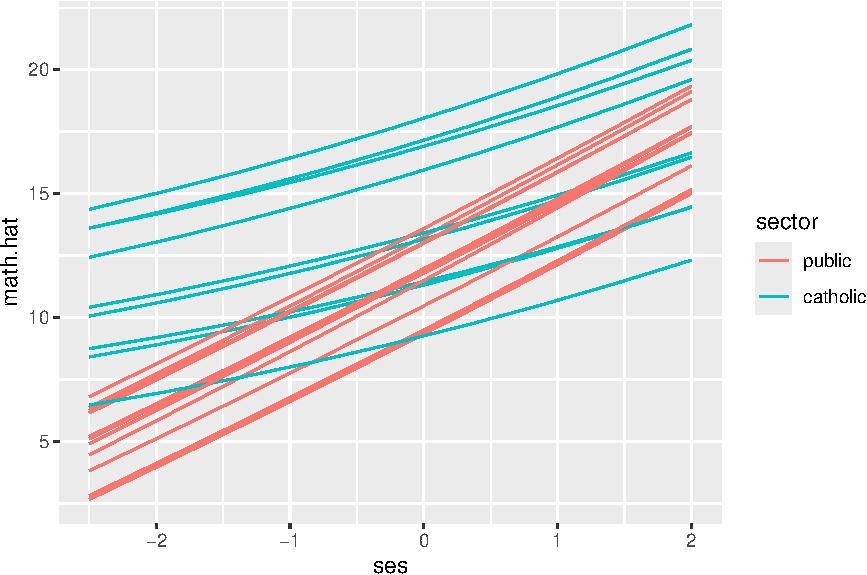
\includegraphics{plot_expand_grid_files/figure-pdf/unnamed-chunk-24-1.pdf}

}

\end{figure}

This code is the same as above. The prediction handles all our model
complexity for us.

Again, we have our equally spaced students:

\begin{Shaded}
\begin{Highlighting}[]
\FunctionTok{ggplot}\NormalTok{( synth.dat}\FloatTok{.20}\NormalTok{, }\FunctionTok{aes}\NormalTok{( ses, math.hat, }\AttributeTok{group=}\NormalTok{id, }\AttributeTok{col=}\NormalTok{sector ) ) }\SpecialCharTok{+}
  \FunctionTok{geom\_line}\NormalTok{() }\SpecialCharTok{+}
  \FunctionTok{geom\_point}\NormalTok{()}
\end{Highlighting}
\end{Shaded}

\begin{figure}[H]

{\centering 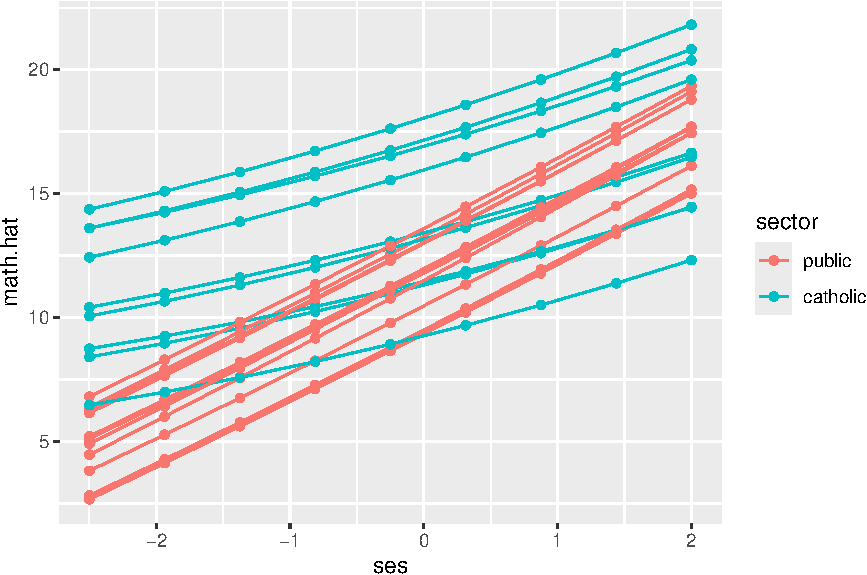
\includegraphics{plot_expand_grid_files/figure-pdf/unnamed-chunk-25-1.pdf}

}

\end{figure}

\hypertarget{longitudinal-data-1}{%
\section{Longitudinal Data}\label{longitudinal-data-1}}

We next do the above, but for longitudinal data. The story is basically
the same.

\hypertarget{the-data}{%
\subsection{The data}\label{the-data}}

We use the ``US Sustaining Effects Study'' taken from Raudenbush and
Bryk (we have not seen these data in class). We have kids in grades
nested in schools. So longitudinal data with a clustering on top of
that.

\begin{Shaded}
\begin{Highlighting}[]
\FunctionTok{head}\NormalTok{( dat )}
\end{Highlighting}
\end{Shaded}

\begin{verbatim}
       CHILDID     SCHOOLID YEAR GRADE   MATH FEMALE SIZE RACEETH
1 101480302    3440         -0.5     1 -1.694      1  588   black
2 101480302    3440          0.5     2 -0.211      1  588   black
3 101480302    3440          1.5     3 -0.403      1  588   black
4 101480302    3440          2.5     4  0.501      1  588   black
5 173559292    2820         -0.5     1 -0.194      0  678   white
6 173559292    2820          0.5     2  2.140      0  678   white
\end{verbatim}

\hypertarget{a-model}{%
\subsection{A model}\label{a-model}}

We will be using the following 3-level quadradic growth model:

\begin{Shaded}
\begin{Highlighting}[]
\NormalTok{M4 }\OtherTok{=} \FunctionTok{lmer}\NormalTok{( MATH }\SpecialCharTok{\textasciitilde{}} \DecValTok{1} \SpecialCharTok{+}\NormalTok{ (YEAR }\SpecialCharTok{+} \FunctionTok{I}\NormalTok{(YEAR}\SpecialCharTok{\^{}}\DecValTok{2}\NormalTok{)) }\SpecialCharTok{*}\NormalTok{ (FEMALE }\SpecialCharTok{*}\NormalTok{ RACEETH ) }\SpecialCharTok{+} 
\NormalTok{                (YEAR}\SpecialCharTok{|}\NormalTok{CHILDID}\SpecialCharTok{:}\NormalTok{SCHOOLID) }\SpecialCharTok{+}\NormalTok{ (YEAR}\SpecialCharTok{|}\NormalTok{SCHOOLID), }\AttributeTok{data=}\NormalTok{dat )}
\FunctionTok{display}\NormalTok{( M4 )}
\end{Highlighting}
\end{Shaded}

\begin{verbatim}
lmer(formula = MATH ~ 1 + (YEAR + I(YEAR^2)) * (FEMALE * RACEETH) + 
    (YEAR | CHILDID:SCHOOLID) + (YEAR | SCHOOLID), data = dat)
                                 coef.est coef.se
(Intercept)                      -0.90     0.06  
YEAR                              0.76     0.02  
I(YEAR^2)                        -0.04     0.01  
FEMALE                            0.02     0.05  
RACEETHhispanic                   0.23     0.10  
RACEETHwhite                      0.79     0.10  
FEMALE:RACEETHhispanic           -0.01     0.12  
FEMALE:RACEETHwhite              -0.34     0.12  
YEAR:FEMALE                       0.01     0.02  
YEAR:RACEETHhispanic              0.10     0.03  
YEAR:RACEETHwhite                 0.07     0.03  
I(YEAR^2):FEMALE                  0.01     0.01  
I(YEAR^2):RACEETHhispanic        -0.01     0.01  
I(YEAR^2):RACEETHwhite           -0.02     0.01  
YEAR:FEMALE:RACEETHhispanic      -0.01     0.04  
YEAR:FEMALE:RACEETHwhite         -0.02     0.04  
I(YEAR^2):FEMALE:RACEETHhispanic  0.00     0.02  
I(YEAR^2):FEMALE:RACEETHwhite     0.02     0.02  

Error terms:
 Groups           Name        Std.Dev. Corr 
 CHILDID:SCHOOLID (Intercept) 0.79          
                  YEAR        0.11     0.55 
 SCHOOLID         (Intercept) 0.34          
                  YEAR        0.10     0.31 
 Residual                     0.54          
---
number of obs: 7230, groups: CHILDID:SCHOOLID, 1721; SCHOOLID, 60
AIC = 16259.7, DIC = 16009.6
deviance = 16109.7 
\end{verbatim}

We are just taking the model as given; this document is about showing
the fit of this model. In particular, if you haven't seen 3-level models
before, just consider the above as some complex model; the nice thing
about \texttt{predict()} is you don't even need to understand the model
you are using! Note we do have a lot of fixed effect interaction terms,
allowing for systematically different trajectories for groups of kids
that are grouped on recorded race and gender.

\hypertarget{the-simple-predict-approach}{%
\subsection{The simple predict()
approach}\label{the-simple-predict-approach}}

We can use our model to predict outcomes for each timepoint in the data.
This will smooth out the time to time variation.

\begin{Shaded}
\begin{Highlighting}[]
\NormalTok{dat}\SpecialCharTok{$}\NormalTok{Yhat }\OtherTok{=} \FunctionTok{predict}\NormalTok{( M4 )}
\FunctionTok{ggplot}\NormalTok{( dat, }\FunctionTok{aes}\NormalTok{( YEAR, Yhat, }\AttributeTok{group=}\NormalTok{CHILDID ) ) }\SpecialCharTok{+}
  \FunctionTok{facet\_grid}\NormalTok{( RACEETH }\SpecialCharTok{\textasciitilde{}}\NormalTok{ FEMALE ) }\SpecialCharTok{+}
  \FunctionTok{geom\_line}\NormalTok{( }\AttributeTok{alpha=}\FloatTok{0.25}\NormalTok{ )}
\end{Highlighting}
\end{Shaded}

\begin{figure}[H]

{\centering \includegraphics{plot_expand_grid_files/figure-pdf/unnamed-chunk-28-1.pdf}

}

\end{figure}

Note how the growth lines don't go across all years for all kids. This
is because we were missing data for those kids in the original dataset
at those timepoints, so we didn't predict outcomes when we used the
\texttt{predict()} function, above.

To fix this we will add in those missing timepoints so we get
predictions for all kids for all timepoints.

\hypertarget{the-expand.grid-function}{%
\subsection{The expand.grid() function}\label{the-expand.grid-function}}

We now want different trajectories for the different groups. We can
generate fake children of each group for each school using
\texttt{expand.grid()}. This method will generate a dataframe with all
combinations of the given variables supplied. Here we make all
combinations of year, gender, and race/ethnic group for each school.

\begin{Shaded}
\begin{Highlighting}[]
\NormalTok{synth.dat }\OtherTok{=} \FunctionTok{expand.grid}\NormalTok{( }\AttributeTok{CHILDID =} \SpecialCharTok{{-}}\DecValTok{1}\NormalTok{,}
                         \AttributeTok{SCHOOLID =} \FunctionTok{levels}\NormalTok{( dat}\SpecialCharTok{$}\NormalTok{SCHOOLID ),}
                         \AttributeTok{YEAR =} \FunctionTok{unique}\NormalTok{( dat}\SpecialCharTok{$}\NormalTok{YEAR ),}
                         \AttributeTok{FEMALE =} \FunctionTok{c}\NormalTok{( }\DecValTok{0}\NormalTok{, }\DecValTok{1}\NormalTok{ ),}
                         \AttributeTok{RACEETH =} \FunctionTok{levels}\NormalTok{( dat}\SpecialCharTok{$}\NormalTok{RACEETH ) )}
\FunctionTok{head}\NormalTok{( synth.dat )}
\end{Highlighting}
\end{Shaded}

\begin{verbatim}
  CHILDID     SCHOOLID YEAR FEMALE RACEETH
1      -1 2020         -0.5      0   black
2      -1 2040         -0.5      0   black
3      -1 2180         -0.5      0   black
4      -1 2330         -0.5      0   black
5      -1 2340         -0.5      0   black
6      -1 2380         -0.5      0   black
\end{verbatim}

\begin{Shaded}
\begin{Highlighting}[]
\FunctionTok{nrow}\NormalTok{( synth.dat )}
\end{Highlighting}
\end{Shaded}

\begin{verbatim}
[1] 2160
\end{verbatim}

The \texttt{CHILDID\ =\ -1} line means we are making up a new child (not
using one of the real ones) so the child random effects will be set to 0
in the predictions.

Once we have our dataset, we use predict to calculate the predicted
outcomes for each student type for each year timepoint for each school:

\begin{Shaded}
\begin{Highlighting}[]
\NormalTok{synth.dat }\OtherTok{=} \FunctionTok{mutate}\NormalTok{( synth.dat, }\AttributeTok{MATH =} \FunctionTok{predict}\NormalTok{( M4, }
                                               \AttributeTok{newdata=}\NormalTok{synth.dat,}
                                               \AttributeTok{allow.new.levels =} \ConstantTok{TRUE}\NormalTok{) )}
\end{Highlighting}
\end{Shaded}

Now we can plot with our new predictions

\begin{Shaded}
\begin{Highlighting}[]
\FunctionTok{ggplot}\NormalTok{( synth.dat, }\FunctionTok{aes}\NormalTok{( YEAR, MATH, }\AttributeTok{group=}\NormalTok{SCHOOLID ) ) }\SpecialCharTok{+}
  \FunctionTok{facet\_grid}\NormalTok{( RACEETH }\SpecialCharTok{\textasciitilde{}}\NormalTok{ FEMALE ) }\SpecialCharTok{+}
  \FunctionTok{geom\_line}\NormalTok{( }\AttributeTok{alpha=}\FloatTok{0.5}\NormalTok{ )}
\end{Highlighting}
\end{Shaded}

\begin{figure}[H]

{\centering \includegraphics{plot_expand_grid_files/figure-pdf/unnamed-chunk-31-1.pdf}

}

\end{figure}

Here we are seeing the different school trajectories for the six types
of kid defined by our student-level demographics.

Or, for a subset of schools

\begin{Shaded}
\begin{Highlighting}[]
\NormalTok{synth.dat }\OtherTok{=} \FunctionTok{mutate}\NormalTok{( synth.dat, }\AttributeTok{GENDER =} \FunctionTok{ifelse}\NormalTok{( FEMALE, }\StringTok{"female"}\NormalTok{, }\StringTok{"male"}\NormalTok{ ) )}
\NormalTok{keepers }\OtherTok{=} \FunctionTok{sample}\NormalTok{( }\FunctionTok{unique}\NormalTok{( synth.dat}\SpecialCharTok{$}\NormalTok{SCHOOLID ), }\DecValTok{12}\NormalTok{ )}
\NormalTok{s2 }\OtherTok{=} \FunctionTok{filter}\NormalTok{( synth.dat, SCHOOLID }\SpecialCharTok{\%in\%}\NormalTok{ keepers )}
\FunctionTok{ggplot}\NormalTok{( s2, }\FunctionTok{aes}\NormalTok{( YEAR, MATH, }\AttributeTok{col=}\NormalTok{RACEETH, }\AttributeTok{lty=}\NormalTok{GENDER ) ) }\SpecialCharTok{+}
  \FunctionTok{facet\_wrap}\NormalTok{( }\SpecialCharTok{\textasciitilde{}}\NormalTok{ SCHOOLID ) }\SpecialCharTok{+}
  \FunctionTok{geom\_line}\NormalTok{( }\AttributeTok{alpha=}\FloatTok{0.5}\NormalTok{) }\SpecialCharTok{+} \FunctionTok{geom\_point}\NormalTok{( }\AttributeTok{alpha=}\FloatTok{0.5}\NormalTok{ )}
\end{Highlighting}
\end{Shaded}

\begin{figure}[H]

{\centering \includegraphics{plot_expand_grid_files/figure-pdf/unnamed-chunk-32-1.pdf}

}

\end{figure}

Here we see the six lines for the six groups within each school, plotted
in little tiles, one for each school.

\hypertarget{population-aggregation}{%
\subsection{Population aggregation}\label{population-aggregation}}

You can also aggregate these predictions. This is the easiest way to get
what collection of schools, averaging over their random effects, looks
like.

Aggregate with the \texttt{group\_by()} and the \texttt{summarise()}
methods:

\begin{Shaded}
\begin{Highlighting}[]
\NormalTok{agg.dat }\OtherTok{=}\NormalTok{ synth.dat }\SpecialCharTok{\%\textgreater{}\%} \FunctionTok{group\_by}\NormalTok{( GENDER, RACEETH, YEAR ) }\SpecialCharTok{\%\textgreater{}\%}
\NormalTok{  dplyr}\SpecialCharTok{::}\FunctionTok{summarise}\NormalTok{( }\AttributeTok{MATH =} \FunctionTok{mean}\NormalTok{( MATH ) )}
\end{Highlighting}
\end{Shaded}

\begin{verbatim}
`summarise()` has grouped output by 'GENDER', 'RACEETH'. You can override using
the `.groups` argument.
\end{verbatim}

\begin{Shaded}
\begin{Highlighting}[]
\FunctionTok{ggplot}\NormalTok{( agg.dat, }\FunctionTok{aes}\NormalTok{( YEAR, MATH, }\AttributeTok{col=}\NormalTok{RACEETH, }\AttributeTok{lty=}\NormalTok{GENDER ) ) }\SpecialCharTok{+}
  \FunctionTok{geom\_line}\NormalTok{( }\AttributeTok{alpha=}\FloatTok{0.5}\NormalTok{) }\SpecialCharTok{+} \FunctionTok{geom\_point}\NormalTok{( }\AttributeTok{alpha=}\FloatTok{0.5}\NormalTok{ )}
\end{Highlighting}
\end{Shaded}

\begin{figure}[H]

{\centering \includegraphics{plot_expand_grid_files/figure-pdf/unnamed-chunk-33-1.pdf}

}

\end{figure}

Or do this via predict directly, using the prior ideas

\begin{Shaded}
\begin{Highlighting}[]
\NormalTok{synth.dat.agg }\OtherTok{=} \FunctionTok{expand.grid}\NormalTok{( }\AttributeTok{CHILDID =} \SpecialCharTok{{-}}\DecValTok{1}\NormalTok{,}
                             \AttributeTok{SCHOOLID =} \SpecialCharTok{{-}}\DecValTok{1}\NormalTok{,}
                             \AttributeTok{YEAR =} \FunctionTok{unique}\NormalTok{( dat}\SpecialCharTok{$}\NormalTok{YEAR ),}
                             \AttributeTok{FEMALE =} \FunctionTok{c}\NormalTok{( }\DecValTok{0}\NormalTok{, }\DecValTok{1}\NormalTok{ ),}
                             \AttributeTok{RACEETH =} \FunctionTok{levels}\NormalTok{( dat}\SpecialCharTok{$}\NormalTok{RACEETH ) )}
\FunctionTok{nrow}\NormalTok{( synth.dat.agg )}
\end{Highlighting}
\end{Shaded}

\begin{verbatim}
[1] 36
\end{verbatim}

\begin{Shaded}
\begin{Highlighting}[]
\NormalTok{synth.dat.agg }\OtherTok{=} \FunctionTok{mutate}\NormalTok{( synth.dat.agg, }
                        \AttributeTok{MATH =} \FunctionTok{predict}\NormalTok{( M4, }
                                        \AttributeTok{newdata=}\NormalTok{synth.dat.agg,}
                                        \AttributeTok{allow.new.levels =} \ConstantTok{TRUE}\NormalTok{) )}
\NormalTok{synth.dat.agg }\OtherTok{=} \FunctionTok{mutate}\NormalTok{( synth.dat.agg, }\AttributeTok{GENDER =} \FunctionTok{ifelse}\NormalTok{( FEMALE, }\StringTok{"female"}\NormalTok{, }\StringTok{"male"}\NormalTok{ ) )}

\FunctionTok{ggplot}\NormalTok{( synth.dat.agg, }\FunctionTok{aes}\NormalTok{( YEAR, MATH, }\AttributeTok{col=}\NormalTok{RACEETH, }\AttributeTok{lty=}\NormalTok{GENDER ) ) }\SpecialCharTok{+}
  \FunctionTok{geom\_line}\NormalTok{( }\AttributeTok{alpha=}\FloatTok{0.5}\NormalTok{) }\SpecialCharTok{+} \FunctionTok{geom\_point}\NormalTok{( }\AttributeTok{alpha=}\FloatTok{0.5}\NormalTok{ )}
\end{Highlighting}
\end{Shaded}

\begin{figure}[H]

{\centering \includegraphics{plot_expand_grid_files/figure-pdf/unnamed-chunk-34-1.pdf}

}

\end{figure}

The above plot suggests that the gender gap only exists for the white
children. It also shows that there are racial gaps, and that the Black
children appear to be falling further behind as time passes.

This block of code is stand-alone, showing the making of fake data and
plotting of predictions all in one go. Especially for glms, where there
are nonlinearities due to the link function, this will give you the
``typical'' units, whereas the aggregation method will average over your
individuals in the sample.

Finally, we can also make tables to calculate observed gaps (although in
many cases you can just read this sort of thing off the regression
table). First \texttt{spread} our data to get columns for each race

\begin{Shaded}
\begin{Highlighting}[]
\NormalTok{s3 }\OtherTok{=} \FunctionTok{spread}\NormalTok{( synth.dat.agg, }\AttributeTok{key=}\StringTok{"RACEETH"}\NormalTok{, }\AttributeTok{value=}\StringTok{"MATH"}\NormalTok{ )}
\FunctionTok{head}\NormalTok{( s3 )}
\end{Highlighting}
\end{Shaded}

\begin{verbatim}
  CHILDID SCHOOLID YEAR FEMALE GENDER     black  hispanic      white
1      -1       -1 -2.5      0   male -3.062597 -3.140761 -2.5729327
2      -1       -1 -2.5      1 female -3.022567 -3.090730 -2.7217865
3      -1       -1 -1.5      0   male -2.129829 -2.071721 -1.4888230
4      -1       -1 -1.5      1 female -2.110196 -2.048891 -1.7416614
5      -1       -1 -0.5      0   male -1.284951 -1.107972 -0.5317700
6      -1       -1 -0.5      1 female -1.268487 -1.096511 -0.8412427
\end{verbatim}

Then summarise:

\begin{Shaded}
\begin{Highlighting}[]
\NormalTok{tab }\OtherTok{=}\NormalTok{ s3 }\SpecialCharTok{\%\textgreater{}\%} \FunctionTok{group\_by}\NormalTok{( YEAR ) }\SpecialCharTok{\%\textgreater{}\%} 
  \FunctionTok{summarise}\NormalTok{( }\AttributeTok{gap.black.white =} \FunctionTok{mean}\NormalTok{( white ) }\SpecialCharTok{{-}} \FunctionTok{mean}\NormalTok{( black ),}
             \AttributeTok{gap.hispanic.white =} \FunctionTok{mean}\NormalTok{( white ) }\SpecialCharTok{{-}} \FunctionTok{mean}\NormalTok{( hispanic ),}
             \AttributeTok{gap.black.hispanic =} \FunctionTok{mean}\NormalTok{( hispanic ) }\SpecialCharTok{{-}} \FunctionTok{mean}\NormalTok{( black ) )}
\NormalTok{knitr}\SpecialCharTok{::}\FunctionTok{kable}\NormalTok{( tab, }\AttributeTok{digits=}\DecValTok{2}\NormalTok{ )}
\end{Highlighting}
\end{Shaded}

\begin{longtable}[]{@{}rrrr@{}}
\toprule\noalign{}
YEAR & gap.black.white & gap.hispanic.white & gap.black.hispanic \\
\midrule\noalign{}
\endhead
\bottomrule\noalign{}
\endlastfoot
-2.5 & 0.40 & 0.47 & -0.07 \\
-1.5 & 0.50 & 0.45 & 0.06 \\
-0.5 & 0.59 & 0.42 & 0.17 \\
0.5 & 0.65 & 0.38 & 0.27 \\
1.5 & 0.69 & 0.34 & 0.35 \\
2.5 & 0.70 & 0.29 & 0.41 \\
\end{longtable}

This again shows widening gap between Black and White students, and the
closing gap of Hispanic and White students.

\hypertarget{plotting-random-effects-by-level-2-variable}{%
\subsection{Plotting random effects by Level 2
variable}\label{plotting-random-effects-by-level-2-variable}}

You can also look at estimated random effects as a function of level 2
variables. For example, we can see if there is a pattern of average math
score for students by year.

\begin{Shaded}
\begin{Highlighting}[]
\NormalTok{ranef }\OtherTok{=} \FunctionTok{ranef}\NormalTok{( M4 )}\SpecialCharTok{$}\NormalTok{SCHOOLID}
\NormalTok{ranef}\SpecialCharTok{$}\NormalTok{SCHOOLID }\OtherTok{=} \FunctionTok{rownames}\NormalTok{( ranef )}
\NormalTok{schools }\OtherTok{=}\NormalTok{ dat }\SpecialCharTok{\%\textgreater{}\%} \FunctionTok{group\_by}\NormalTok{( SCHOOLID ) }\SpecialCharTok{\%\textgreater{}\%}
  \FunctionTok{summarise}\NormalTok{( }\AttributeTok{n =} \FunctionTok{n}\NormalTok{(),}
             \AttributeTok{size =}\NormalTok{ SIZE[[}\DecValTok{1}\NormalTok{]] )}
\NormalTok{schools }\OtherTok{=} \FunctionTok{merge}\NormalTok{( schools, ranef, }\AttributeTok{by=}\StringTok{"SCHOOLID"}\NormalTok{ )}
\FunctionTok{head}\NormalTok{( schools )}
\end{Highlighting}
\end{Shaded}

\begin{verbatim}
      SCHOOLID   n size (Intercept)        YEAR
1 2020          97  380  0.40323695  0.15257155
2 2040          89  502  0.11549112  0.07547119
3 2180         168  777 -0.08149965 -0.08226575
4 2330         150  800  0.32372001 -0.04389156
5 2340         220 1133 -0.05151492 -0.01128209
6 2380          87  439 -0.17018815  0.10802722
\end{verbatim}

\begin{Shaded}
\begin{Highlighting}[]
\FunctionTok{ggplot}\NormalTok{( schools, }\FunctionTok{aes}\NormalTok{( size, }\StringTok{\textasciigrave{}}\AttributeTok{(Intercept)}\StringTok{\textasciigrave{}}\NormalTok{ ) ) }\SpecialCharTok{+}
  \FunctionTok{geom\_point}\NormalTok{() }\SpecialCharTok{+}
  \FunctionTok{geom\_smooth}\NormalTok{(}\AttributeTok{method=}\StringTok{"lm"}\NormalTok{)}
\end{Highlighting}
\end{Shaded}

\begin{verbatim}
`geom_smooth()` using formula = 'y ~ x'
\end{verbatim}

\begin{figure}[H]

{\centering \includegraphics{plot_expand_grid_files/figure-pdf/unnamed-chunk-37-1.pdf}

}

\end{figure}

We see a possible negative trend.

\hypertarget{easy-graphing-with-ggeffects}{%
\chapter{\texorpdfstring{Easy Graphing with
\texttt{ggeffects}}{Easy Graphing with ggeffects}}\label{easy-graphing-with-ggeffects}}

An awesome convenience function for graphing regression models is the
\texttt{ggeffects} package. It's the best equivalent I've found in R to
Stata's \texttt{margins}. Let's demonstrate with the HSB data.

\begin{Shaded}
\begin{Highlighting}[]
\CommentTok{\# load libraries}
\FunctionTok{library}\NormalTok{(tidyverse)}
\FunctionTok{library}\NormalTok{(lme4)}
\FunctionTok{library}\NormalTok{(ggeffects)}
\FunctionTok{library}\NormalTok{(sjPlot)}
\FunctionTok{library}\NormalTok{(haven)}

\CommentTok{\# clear memory}
\FunctionTok{rm}\NormalTok{(}\AttributeTok{list =} \FunctionTok{ls}\NormalTok{())}

\CommentTok{\# load HSB data}
\NormalTok{hsb }\OtherTok{\textless{}{-}} \FunctionTok{read\_dta}\NormalTok{(}\StringTok{"data/hsb.dta"}\NormalTok{)}
\end{Highlighting}
\end{Shaded}

\hypertarget{fit-a-series-of-models}{%
\section{Fit a Series of Models}\label{fit-a-series-of-models}}

We can fit 2- and 3-way interactions, but they can be hard to interpret
from the coefficients alone (unless you have a lot of practice).

\begin{Shaded}
\begin{Highlighting}[]
\NormalTok{m1 }\OtherTok{\textless{}{-}} \FunctionTok{lmer}\NormalTok{(mathach }\SpecialCharTok{\textasciitilde{}}\NormalTok{ ses }\SpecialCharTok{+}\NormalTok{ (}\DecValTok{1}\SpecialCharTok{|}\NormalTok{schoolid), hsb)}
\NormalTok{m2 }\OtherTok{\textless{}{-}} \FunctionTok{lmer}\NormalTok{(mathach }\SpecialCharTok{\textasciitilde{}}\NormalTok{ ses }\SpecialCharTok{+}\NormalTok{ sector }\SpecialCharTok{+}\NormalTok{ (}\DecValTok{1}\SpecialCharTok{|}\NormalTok{schoolid), hsb)}
\NormalTok{m3 }\OtherTok{\textless{}{-}} \FunctionTok{lmer}\NormalTok{(mathach }\SpecialCharTok{\textasciitilde{}}\NormalTok{ ses}\SpecialCharTok{*}\NormalTok{sector }\SpecialCharTok{+}\NormalTok{ (}\DecValTok{1}\SpecialCharTok{|}\NormalTok{schoolid), hsb)}
\NormalTok{m4 }\OtherTok{\textless{}{-}} \FunctionTok{lmer}\NormalTok{(mathach }\SpecialCharTok{\textasciitilde{}}\NormalTok{ ses}\SpecialCharTok{*}\NormalTok{sector}\SpecialCharTok{*}\NormalTok{female }\SpecialCharTok{+}\NormalTok{ (}\DecValTok{1}\SpecialCharTok{|}\NormalTok{schoolid), hsb)}

\CommentTok{\# tabulate results with tab\_model}
\FunctionTok{tab\_model}\NormalTok{(m1, m2, m3, m4,}
          \AttributeTok{p.style =} \StringTok{"stars"}\NormalTok{,}
          \AttributeTok{show.ci =} \ConstantTok{FALSE}\NormalTok{,}
          \AttributeTok{show.se =} \ConstantTok{TRUE}\NormalTok{)}
\end{Highlighting}
\end{Shaded}

~

mathach

mathach

mathach

mathach

Predictors

Estimates

std. Error

Estimates

std. Error

Estimates

std. Error

Estimates

std. Error

(Intercept)

12.66 \textsuperscript{***}

0.19

11.72 \textsuperscript{***}

0.23

11.80 \textsuperscript{***}

0.23

12.41 \textsuperscript{***}

0.25

ses

2.39 \textsuperscript{***}

0.11

2.37 \textsuperscript{***}

0.11

2.95 \textsuperscript{***}

0.14

2.73 \textsuperscript{***}

0.19

sector

2.10 \textsuperscript{***}

0.34

2.14 \textsuperscript{***}

0.34

2.16 \textsuperscript{***}

0.38

ses × sector

-1.31 \textsuperscript{***}

0.21

-1.26 \textsuperscript{***}

0.30

female

-1.16 \textsuperscript{***}

0.21

ses × female

0.34 \textsuperscript{}

0.26

sector × female

-0.05 \textsuperscript{}

0.35

(ses × sector) × female

-0.05 \textsuperscript{}

0.40

Random Effects

σ\textsuperscript{2}

37.03

37.04

36.84

36.63

τ\textsubscript{00}

4.77 \textsubscript{schoolid}

3.69 \textsubscript{schoolid}

3.69 \textsubscript{schoolid}

3.40 \textsubscript{schoolid}

ICC

0.11

0.09

0.09

0.09

N

160 \textsubscript{schoolid}

160 \textsubscript{schoolid}

160 \textsubscript{schoolid}

160 \textsubscript{schoolid}

Observations

7185

7185

7185

7185

Marginal R\textsuperscript{2} / Conditional R\textsuperscript{2}

0.077 / 0.182

0.114 / 0.195

0.118 / 0.199

0.127 / 0.202

* p\textless0.05~~~** p\textless0.01~~~*** p\textless0.001

\hypertarget{graph-the-results-with-ggeffects}{%
\section{\texorpdfstring{Graph the Results with
\texttt{ggeffects}}{Graph the Results with ggeffects}}\label{graph-the-results-with-ggeffects}}

If we just call \texttt{ggeffect} on the model object, we get a bunch of
predicted values:

\begin{Shaded}
\begin{Highlighting}[]
\FunctionTok{ggeffect}\NormalTok{(m1)}
\end{Highlighting}
\end{Shaded}

\begin{verbatim}
$ses
# Predicted values of mathach

ses | Predicted |         95% CI
--------------------------------
 -4 |      3.10 | [ 2.19,  4.00]
 -3 |      5.49 | [ 4.77,  6.21]
 -2 |      7.88 | [ 7.32,  8.43]
 -1 |     10.27 | [ 9.85, 10.69]
  0 |     12.66 | [12.29, 13.03]
  1 |     15.05 | [14.62, 15.47]
  2 |     17.44 | [16.88, 17.99]
  3 |     19.83 | [19.10, 20.55]

attr(,"class")
[1] "ggalleffects" "list"        
attr(,"model.name")
[1] "m1"
\end{verbatim}

We can pipe that into \texttt{plot} to get a nice plot:

\begin{Shaded}
\begin{Highlighting}[]
\FunctionTok{ggeffect}\NormalTok{(m1) }\SpecialCharTok{|\textgreater{}} 
  \FunctionTok{plot}\NormalTok{()}
\end{Highlighting}
\end{Shaded}

\begin{verbatim}
$ses
\end{verbatim}

\begin{figure}[H]

{\centering \includegraphics{ggeffects_files/figure-pdf/unnamed-chunk-5-1.pdf}

}

\end{figure}

With multiple covariates, we can call the \texttt{terms} argument. The
first input is on X, the second is mapped to color, the third to facet.
This makes visualizing the interactions super easy! Any covariates
included in the model but not included in \texttt{terms} are held
constant at their means.

\begin{Shaded}
\begin{Highlighting}[]
\FunctionTok{ggeffect}\NormalTok{(m2, }\AttributeTok{terms =} \FunctionTok{c}\NormalTok{(}\StringTok{"ses"}\NormalTok{, }\StringTok{"sector"}\NormalTok{)) }\SpecialCharTok{|\textgreater{}} 
  \FunctionTok{plot}\NormalTok{(}\AttributeTok{ci =} \ConstantTok{FALSE}\NormalTok{, }\AttributeTok{add.data =} \ConstantTok{TRUE}\NormalTok{)}
\end{Highlighting}
\end{Shaded}

\begin{figure}[H]

{\centering \includegraphics{ggeffects_files/figure-pdf/unnamed-chunk-6-1.pdf}

}

\end{figure}

\begin{Shaded}
\begin{Highlighting}[]
\FunctionTok{ggeffect}\NormalTok{(m3, }\AttributeTok{terms =} \FunctionTok{c}\NormalTok{(}\StringTok{"ses"}\NormalTok{, }\StringTok{"sector"}\NormalTok{)) }\SpecialCharTok{|\textgreater{}} 
  \FunctionTok{plot}\NormalTok{(}\AttributeTok{ci =} \ConstantTok{FALSE}\NormalTok{)}
\end{Highlighting}
\end{Shaded}

\begin{figure}[H]

{\centering \includegraphics{ggeffects_files/figure-pdf/unnamed-chunk-6-2.pdf}

}

\end{figure}

\begin{Shaded}
\begin{Highlighting}[]
\FunctionTok{ggeffect}\NormalTok{(m4, }\AttributeTok{terms =} \FunctionTok{c}\NormalTok{(}\StringTok{"ses"}\NormalTok{, }\StringTok{"sector"}\NormalTok{, }\StringTok{"female"}\NormalTok{)) }\SpecialCharTok{|\textgreater{}} 
  \FunctionTok{plot}\NormalTok{(}\AttributeTok{ci =} \ConstantTok{FALSE}\NormalTok{)}
\end{Highlighting}
\end{Shaded}

\begin{figure}[H]

{\centering \includegraphics{ggeffects_files/figure-pdf/unnamed-chunk-6-3.pdf}

}

\end{figure}

\hypertarget{plotting-two-datasets-at-once}{%
\chapter{Plotting Two Datasets at
Once}\label{plotting-two-datasets-at-once}}

It's easy (though not always advisable) to plot two data sets at once
with \texttt{ggplot}. First, we load tidyverse and our HSB data. We then
create a school-level aggregate data set of just the mean SES values.

\begin{Shaded}
\begin{Highlighting}[]
\FunctionTok{library}\NormalTok{(tidyverse)}
\FunctionTok{library}\NormalTok{(haven)}

\CommentTok{\# clear memory}
\FunctionTok{rm}\NormalTok{(}\AttributeTok{list =} \FunctionTok{ls}\NormalTok{())}

\FunctionTok{theme\_set}\NormalTok{(}\FunctionTok{theme\_classic}\NormalTok{())}

\CommentTok{\# load HSB data}
\NormalTok{hsb }\OtherTok{\textless{}{-}} \FunctionTok{read\_dta}\NormalTok{(}\StringTok{"data/hsb.dta"}\NormalTok{) }\SpecialCharTok{|\textgreater{}} 
  \FunctionTok{select}\NormalTok{(mathach, ses, schoolid)}

\NormalTok{sch }\OtherTok{\textless{}{-}}\NormalTok{ hsb }\SpecialCharTok{|\textgreater{}} 
  \FunctionTok{group\_by}\NormalTok{(schoolid) }\SpecialCharTok{|\textgreater{}} 
  \FunctionTok{summarise}\NormalTok{(}\AttributeTok{mean\_ses =} \FunctionTok{mean}\NormalTok{(ses),}
            \AttributeTok{mean\_mathach =} \FunctionTok{mean}\NormalTok{(mathach))}
\end{Highlighting}
\end{Shaded}

Let's say we wanted to plot \emph{both} the individual students
\emph{and} the school means. This is easy enough to do separately:

\begin{Shaded}
\begin{Highlighting}[]
\FunctionTok{ggplot}\NormalTok{(hsb, }\FunctionTok{aes}\NormalTok{(}\AttributeTok{x =}\NormalTok{ ses, }\AttributeTok{y =}\NormalTok{ mathach)) }\SpecialCharTok{+}
  \FunctionTok{geom\_point}\NormalTok{(}\AttributeTok{alpha =} \FloatTok{0.1}\NormalTok{)}
\end{Highlighting}
\end{Shaded}

\begin{figure}[H]

{\centering \includegraphics{double_plot_files/figure-pdf/unnamed-chunk-3-1.pdf}

}

\end{figure}

\begin{Shaded}
\begin{Highlighting}[]
\FunctionTok{ggplot}\NormalTok{(sch, }\FunctionTok{aes}\NormalTok{(}\AttributeTok{x =}\NormalTok{ mean\_ses, }\AttributeTok{y =}\NormalTok{ mean\_mathach)) }\SpecialCharTok{+}
  \FunctionTok{geom\_point}\NormalTok{()}
\end{Highlighting}
\end{Shaded}

\begin{figure}[H]

{\centering \includegraphics{double_plot_files/figure-pdf/unnamed-chunk-3-2.pdf}

}

\end{figure}

We can superimpose both plots as follows. Essentially, the first
argument in \texttt{ggplot} provides the data, and by default, this is
passed to all subsequent layers of the plot. We can override this
behavior by specifying a different data set (and aesthetic mappings, if
desired) \emph{within an individual layer} of \texttt{ggplot}, such as
\texttt{geom\_point}.

\begin{Shaded}
\begin{Highlighting}[]
\FunctionTok{ggplot}\NormalTok{(hsb, }\FunctionTok{aes}\NormalTok{(}\AttributeTok{x =}\NormalTok{ ses, }\AttributeTok{y =}\NormalTok{ mathach)) }\SpecialCharTok{+}
  \FunctionTok{geom\_point}\NormalTok{(}\AttributeTok{alpha =} \FloatTok{0.1}\NormalTok{) }\SpecialCharTok{+}
  \FunctionTok{geom\_point}\NormalTok{(}\AttributeTok{data =}\NormalTok{ sch, }\FunctionTok{aes}\NormalTok{(}\AttributeTok{x =}\NormalTok{ mean\_ses, }\AttributeTok{y =}\NormalTok{ mean\_mathach), }\AttributeTok{color =} \StringTok{"red"}\NormalTok{)}
\end{Highlighting}
\end{Shaded}

\begin{figure}[H]

{\centering \includegraphics{double_plot_files/figure-pdf/unnamed-chunk-4-1.pdf}

}

\end{figure}

\part{MODEL FITTING \& INTERPRETATION}

\hypertarget{extracting-model-information-with-broom}{%
\chapter{\texorpdfstring{Extracting model information with
\texttt{broom}}{Extracting model information with broom}}\label{extracting-model-information-with-broom}}

There are three general ways to get information out of a fit model: (1)
print it to the screen and read it, (2) use a variety of base R methods
to pull information out of the model, and (2) use the \texttt{broom}
package to pull information out of the model into different kinds of
data frames (which is in line with \emph{tidy programming}, and the
tidyverse).

This chapter looks at the third way. The following chapter looks at the
``base R'' way. Which to use is a matter of preference.

\hypertarget{simple-demonstration}{%
\section{Simple Demonstration}\label{simple-demonstration}}

One of my favorite R packages is \texttt{broom}, which has many awesome
convenience functions for regression models, including MLMs.
\texttt{broom.mixed} is the extension that specifically works with
\texttt{lmer} models. It does this via a few core methods that give you
the model parameters and information as a nice data frame that you can
then use more easily than the original result from your \texttt{lmer()}
call. Let's see how it works.

We first load it (and a few other things, and some data):

\begin{Shaded}
\begin{Highlighting}[]
\CommentTok{\# load libraries}
\FunctionTok{library}\NormalTok{(tidyverse)}
\FunctionTok{library}\NormalTok{(broom.mixed)}
\FunctionTok{library}\NormalTok{(haven)}
\FunctionTok{library}\NormalTok{(knitr)}
\FunctionTok{library}\NormalTok{(lme4)}

\CommentTok{\# clear memory}
\FunctionTok{rm}\NormalTok{(}\AttributeTok{list =} \FunctionTok{ls}\NormalTok{())}

\CommentTok{\# load HSB data}
\NormalTok{hsb }\OtherTok{\textless{}{-}} \FunctionTok{read\_dta}\NormalTok{(}\StringTok{"data/hsb.dta"}\NormalTok{)}
\end{Highlighting}
\end{Shaded}

\hypertarget{tidy}{%
\subsection{\texorpdfstring{\texttt{tidy}}{tidy}}\label{tidy}}

The \texttt{tidy()} method takes a model object and returns the output
as a tidy tibble (i.e., a data frame), which makes it very easy to work
with. Compare the results below:

\begin{Shaded}
\begin{Highlighting}[]
\NormalTok{ols }\OtherTok{\textless{}{-}} \FunctionTok{lm}\NormalTok{(mathach }\SpecialCharTok{\textasciitilde{}}\NormalTok{ ses, hsb)}

\CommentTok{\# ugly!}
\FunctionTok{summary}\NormalTok{(ols)}
\end{Highlighting}
\end{Shaded}

\begin{verbatim}

Call:
lm(formula = mathach ~ ses, data = hsb)

Residuals:
     Min       1Q   Median       3Q      Max 
-19.4382  -4.7580   0.2334   5.0649  15.9007 

Coefficients:
            Estimate Std. Error t value Pr(>|t|)    
(Intercept) 12.74740    0.07569  168.42   <2e-16 ***
ses          3.18387    0.09712   32.78   <2e-16 ***
---
Signif. codes:  0 '***' 0.001 '**' 0.01 '*' 0.05 '.' 0.1 ' ' 1

Residual standard error: 6.416 on 7183 degrees of freedom
Multiple R-squared:  0.1301,    Adjusted R-squared:   0.13 
F-statistic:  1075 on 1 and 7183 DF,  p-value: < 2.2e-16
\end{verbatim}

\begin{Shaded}
\begin{Highlighting}[]
\CommentTok{\# beautiful!}
\FunctionTok{tidy}\NormalTok{(ols)}
\end{Highlighting}
\end{Shaded}

\begin{verbatim}
# A tibble: 2 x 5
  term        estimate std.error statistic   p.value
  <chr>          <dbl>     <dbl>     <dbl>     <dbl>
1 (Intercept)    12.7     0.0757     168.  0        
2 ses             3.18    0.0971      32.8 8.71e-220
\end{verbatim}

\begin{Shaded}
\begin{Highlighting}[]
\CommentTok{\# even better}
\NormalTok{ols }\SpecialCharTok{|\textgreater{}} \FunctionTok{tidy}\NormalTok{() }\SpecialCharTok{|\textgreater{}} \FunctionTok{kable}\NormalTok{(}\AttributeTok{digits =} \DecValTok{2}\NormalTok{)}
\end{Highlighting}
\end{Shaded}

\begin{longtable}[]{@{}lrrrr@{}}
\toprule\noalign{}
term & estimate & std.error & statistic & p.value \\
\midrule\noalign{}
\endhead
\bottomrule\noalign{}
\endlastfoot
(Intercept) & 12.75 & 0.08 & 168.42 & 0 \\
ses & 3.18 & 0.10 & 32.78 & 0 \\
\end{longtable}

\begin{Shaded}
\begin{Highlighting}[]
\CommentTok{\# Also works great for MLMs}
\NormalTok{mlm }\OtherTok{\textless{}{-}} \FunctionTok{lmer}\NormalTok{(mathach }\SpecialCharTok{\textasciitilde{}}\NormalTok{ ses }\SpecialCharTok{+}\NormalTok{ mnses }\SpecialCharTok{+}\NormalTok{ (ses}\SpecialCharTok{|}\NormalTok{schoolid), hsb)}

\FunctionTok{tidy}\NormalTok{(mlm)}
\end{Highlighting}
\end{Shaded}

\begin{verbatim}
# A tibble: 7 x 6
  effect   group    term                 estimate std.error statistic
  <chr>    <chr>    <chr>                   <dbl>     <dbl>     <dbl>
1 fixed    <NA>     (Intercept)            12.7       0.151     84.2 
2 fixed    <NA>     ses                     2.19      0.122     18.0 
3 fixed    <NA>     mnses                   3.78      0.383      9.88
4 ran_pars schoolid sd__(Intercept)         1.64     NA         NA   
5 ran_pars schoolid cor__(Intercept).ses   -0.212    NA         NA   
6 ran_pars schoolid sd__ses                 0.673    NA         NA   
7 ran_pars Residual sd__Observation         6.07     NA         NA   
\end{verbatim}

\hypertarget{glance}{%
\subsection{\texorpdfstring{\texttt{glance}}{glance}}\label{glance}}

What about model fit stats? That's where \texttt{glance} comes in:

\begin{Shaded}
\begin{Highlighting}[]
\FunctionTok{glance}\NormalTok{(ols)}
\end{Highlighting}
\end{Shaded}

\begin{verbatim}
# A tibble: 1 x 12
  r.squared adj.r.squared sigma statistic   p.value    df  logLik    AIC    BIC
      <dbl>         <dbl> <dbl>     <dbl>     <dbl> <dbl>   <dbl>  <dbl>  <dbl>
1     0.130         0.130  6.42     1075. 8.71e-220     1 -23549. 47104. 47125.
# i 3 more variables: deviance <dbl>, df.residual <int>, nobs <int>
\end{verbatim}

\begin{Shaded}
\begin{Highlighting}[]
\FunctionTok{glance}\NormalTok{(mlm) }\SpecialCharTok{|\textgreater{}} 
  \FunctionTok{kable}\NormalTok{(}\AttributeTok{digits =} \DecValTok{2}\NormalTok{)}
\end{Highlighting}
\end{Shaded}

\begin{longtable}[]{@{}rrrrrrr@{}}
\toprule\noalign{}
nobs & sigma & logLik & AIC & BIC & REMLcrit & df.residual \\
\midrule\noalign{}
\endhead
\bottomrule\noalign{}
\endlastfoot
7185 & 6.07 & -23280.71 & 46575.42 & 46623.58 & 46561.42 & 7178 \\
\end{longtable}

\hypertarget{augment}{%
\subsection{\texorpdfstring{\texttt{augment}}{augment}}\label{augment}}

What about your estimated random effects? \texttt{augment} to the
rescue, giving estimates for each random effect:

\begin{Shaded}
\begin{Highlighting}[]
\NormalTok{mlm }\SpecialCharTok{|\textgreater{}} 
  \FunctionTok{ranef}\NormalTok{() }\SpecialCharTok{|\textgreater{}} 
  \FunctionTok{augment}\NormalTok{() }\SpecialCharTok{|\textgreater{}} 
  \FunctionTok{head}\NormalTok{() }\SpecialCharTok{|\textgreater{}} 
  \FunctionTok{kable}\NormalTok{(}\AttributeTok{digits =} \DecValTok{2}\NormalTok{)}
\end{Highlighting}
\end{Shaded}

\begin{longtable}[]{@{}
  >{\raggedright\arraybackslash}p{(\columnwidth - 14\tabcolsep) * \real{0.1406}}
  >{\raggedright\arraybackslash}p{(\columnwidth - 14\tabcolsep) * \real{0.1875}}
  >{\raggedright\arraybackslash}p{(\columnwidth - 14\tabcolsep) * \real{0.0938}}
  >{\raggedleft\arraybackslash}p{(\columnwidth - 14\tabcolsep) * \real{0.1406}}
  >{\raggedleft\arraybackslash}p{(\columnwidth - 14\tabcolsep) * \real{0.0938}}
  >{\raggedleft\arraybackslash}p{(\columnwidth - 14\tabcolsep) * \real{0.1562}}
  >{\raggedleft\arraybackslash}p{(\columnwidth - 14\tabcolsep) * \real{0.0938}}
  >{\raggedleft\arraybackslash}p{(\columnwidth - 14\tabcolsep) * \real{0.0938}}@{}}
\toprule\noalign{}
\begin{minipage}[b]{\linewidth}\raggedright
grp
\end{minipage} & \begin{minipage}[b]{\linewidth}\raggedright
variable
\end{minipage} & \begin{minipage}[b]{\linewidth}\raggedright
level
\end{minipage} & \begin{minipage}[b]{\linewidth}\raggedleft
estimate
\end{minipage} & \begin{minipage}[b]{\linewidth}\raggedleft
qq
\end{minipage} & \begin{minipage}[b]{\linewidth}\raggedleft
std.error
\end{minipage} & \begin{minipage}[b]{\linewidth}\raggedleft
lb
\end{minipage} & \begin{minipage}[b]{\linewidth}\raggedleft
ub
\end{minipage} \\
\midrule\noalign{}
\endhead
\bottomrule\noalign{}
\endlastfoot
schoolid & (Intercept) & 8367 & -4.14 & -0.18 & 0.78 & -5.43 & -2.85 \\
schoolid & (Intercept) & 4523 & -3.09 & 0.02 & 0.98 & -4.70 & -1.47 \\
schoolid & (Intercept) & 6990 & -2.98 & -1.46 & 0.78 & -4.26 & -1.70 \\
schoolid & (Intercept) & 3705 & -2.81 & 0.28 & 1.09 & -4.61 & -1.02 \\
schoolid & (Intercept) & 8854 & -2.57 & -0.85 & 0.80 & -3.89 & -1.25 \\
schoolid & (Intercept) & 9397 & -2.43 & -0.65 & 0.92 & -3.94 & -0.92 \\
\end{longtable}

The \texttt{level} column are your school IDs, here. If you have
multiple sets of random effects, they will all be stacked, and indexed
via \texttt{grp}.

\hypertarget{extracting-lmer-model-info}{%
\section{\texorpdfstring{Extracting \texttt{lmer} model
info}{Extracting lmer model info}}\label{extracting-lmer-model-info}}

\hypertarget{obtaining-fixed-effects}{%
\subsection{Obtaining Fixed Effects}\label{obtaining-fixed-effects}}

\texttt{lmer} models are in reduced form, so fixed effects include both
L1 and L2 predictors. \texttt{tidy} denotes the type of effect in a
column called \texttt{effect}, where \texttt{fixed} means fixed, and
\texttt{ran\_pars} means random (standing for ``random parameters'')

\begin{Shaded}
\begin{Highlighting}[]
\NormalTok{mlm }\SpecialCharTok{|\textgreater{}} 
  \FunctionTok{tidy}\NormalTok{() }\SpecialCharTok{|\textgreater{}} 
  \FunctionTok{filter}\NormalTok{(effect }\SpecialCharTok{==} \StringTok{"fixed"}\NormalTok{)}
\end{Highlighting}
\end{Shaded}

\begin{verbatim}
# A tibble: 3 x 6
  effect group term        estimate std.error statistic
  <chr>  <chr> <chr>          <dbl>     <dbl>     <dbl>
1 fixed  <NA>  (Intercept)    12.7      0.151     84.2 
2 fixed  <NA>  ses             2.19     0.122     18.0 
3 fixed  <NA>  mnses           3.78     0.383      9.88
\end{verbatim}

We can use the \texttt{{[}{[}{]}{]}} notation or a pipeline to extract
elements from the data frame:

\begin{Shaded}
\begin{Highlighting}[]
\CommentTok{\# within effect of SES}
\FunctionTok{tidy}\NormalTok{(mlm)[[}\DecValTok{2}\NormalTok{,}\DecValTok{4}\NormalTok{]]}
\end{Highlighting}
\end{Shaded}

\begin{verbatim}
[1] 2.190349
\end{verbatim}

\begin{Shaded}
\begin{Highlighting}[]
\CommentTok{\# contextual effect of SES}
\FunctionTok{tidy}\NormalTok{(mlm)[[}\DecValTok{3}\NormalTok{,}\DecValTok{4}\NormalTok{]]}
\end{Highlighting}
\end{Shaded}

\begin{verbatim}
[1] 3.781243
\end{verbatim}

\begin{Shaded}
\begin{Highlighting}[]
\CommentTok{\# using the variable names in a pipeline}
\NormalTok{mlm }\SpecialCharTok{|\textgreater{}} 
  \FunctionTok{tidy}\NormalTok{() }\SpecialCharTok{|\textgreater{}} 
  \FunctionTok{filter}\NormalTok{(term }\SpecialCharTok{==} \StringTok{"ses"}\NormalTok{) }\SpecialCharTok{|\textgreater{}} 
  \FunctionTok{pull}\NormalTok{(estimate)}
\end{Highlighting}
\end{Shaded}

\begin{verbatim}
[1] 2.190349
\end{verbatim}

\hypertarget{obtaining-random-effects}{%
\subsection{Obtaining Random Effects}\label{obtaining-random-effects}}

\texttt{tidy} includes the random effects (SDs and correlations) right
there in the output. For example, \texttt{sd\_\_ses} is the SD of the
SES slope.

\begin{Shaded}
\begin{Highlighting}[]
\CommentTok{\# display all random effects}
\NormalTok{mlm }\SpecialCharTok{|\textgreater{}} 
  \FunctionTok{tidy}\NormalTok{() }\SpecialCharTok{|\textgreater{}} 
  \FunctionTok{filter}\NormalTok{(effect }\SpecialCharTok{==} \StringTok{"ran\_pars"}\NormalTok{)}
\end{Highlighting}
\end{Shaded}

\begin{verbatim}
# A tibble: 4 x 6
  effect   group    term                 estimate std.error statistic
  <chr>    <chr>    <chr>                   <dbl>     <dbl>     <dbl>
1 ran_pars schoolid sd__(Intercept)         1.64         NA        NA
2 ran_pars schoolid cor__(Intercept).ses   -0.212        NA        NA
3 ran_pars schoolid sd__ses                 0.673        NA        NA
4 ran_pars Residual sd__Observation         6.07         NA        NA
\end{verbatim}

\begin{Shaded}
\begin{Highlighting}[]
\CommentTok{\# pull single number}
\NormalTok{mlm }\SpecialCharTok{|\textgreater{}} 
  \FunctionTok{tidy}\NormalTok{() }\SpecialCharTok{|\textgreater{}} 
  \FunctionTok{filter}\NormalTok{(term }\SpecialCharTok{==} \StringTok{"sd\_\_ses"}\NormalTok{) }\SpecialCharTok{|\textgreater{}} 
  \FunctionTok{pull}\NormalTok{(estimate)}
\end{Highlighting}
\end{Shaded}

\begin{verbatim}
[1] 0.6730818
\end{verbatim}

\hypertarget{obtaining-empirical-bayes-estimates-of-the-random-effects}{%
\subsection{Obtaining Empirical Bayes Estimates of the Random
Effects}\label{obtaining-empirical-bayes-estimates-of-the-random-effects}}

This is best done in a pipeline. We first apply \texttt{ranef}, then
\texttt{augment} and get the EB estimates in the \texttt{estimate}
column, along with the \texttt{std.error}, confidence bounds, and
\texttt{qq} statistics.

\begin{Shaded}
\begin{Highlighting}[]
\NormalTok{mlm }\SpecialCharTok{|\textgreater{}} 
  \FunctionTok{ranef}\NormalTok{() }\SpecialCharTok{|\textgreater{}} 
  \FunctionTok{augment}\NormalTok{() }\SpecialCharTok{|\textgreater{}} 
  \FunctionTok{head}\NormalTok{()}
\end{Highlighting}
\end{Shaded}

\begin{verbatim}
       grp    variable level  estimate         qq std.error        lb
1 schoolid (Intercept)  8367 -4.137656 -0.1811498 0.7845770 -5.428170
2 schoolid (Intercept)  4523 -3.089835  0.0235018 0.9819306 -4.704967
3 schoolid (Intercept)  6990 -2.981315 -1.4619679 0.7779876 -4.260991
4 schoolid (Intercept)  3705 -2.811935  0.2776904 1.0911916 -4.606785
5 schoolid (Intercept)  8854 -2.569302 -0.8528365 0.8045804 -3.892719
6 schoolid (Intercept)  9397 -2.431031 -0.6452734 0.9163587 -3.938307
          ub
1 -2.8471413
2 -1.4747032
3 -1.7016394
4 -1.0170840
5 -1.2458846
6 -0.9237553
\end{verbatim}

\hypertarget{intercept-slope-correlation}{%
\subsection{Intercept-Slope
Correlation}\label{intercept-slope-correlation}}

The BLUPs are in long form. We can reshape to wide if we want to, for
example, visualize the correlation between the random intercepts and
slopes.

\begin{Shaded}
\begin{Highlighting}[]
\NormalTok{blups }\OtherTok{\textless{}{-}}\NormalTok{ mlm }\SpecialCharTok{|\textgreater{}} 
  \FunctionTok{ranef}\NormalTok{() }\SpecialCharTok{|\textgreater{}} 
  \FunctionTok{augment}\NormalTok{() }\SpecialCharTok{|\textgreater{}} 
\NormalTok{  dplyr}\SpecialCharTok{::}\FunctionTok{select}\NormalTok{(variable, level, estimate) }\SpecialCharTok{|\textgreater{}} 
  \FunctionTok{pivot\_wider}\NormalTok{(}\AttributeTok{names\_from =}\NormalTok{ variable, }\AttributeTok{values\_from =}\NormalTok{ estimate,}
              \AttributeTok{id\_cols =}\NormalTok{ level) }\SpecialCharTok{|\textgreater{}} 
\NormalTok{  dplyr}\SpecialCharTok{::}\FunctionTok{rename}\NormalTok{(}\AttributeTok{schoolid =} \DecValTok{1}\NormalTok{, }\AttributeTok{random\_intercept =} \DecValTok{2}\NormalTok{, }\AttributeTok{random\_slope =} \DecValTok{3}\NormalTok{)}

\FunctionTok{head}\NormalTok{(blups)}
\end{Highlighting}
\end{Shaded}

\begin{verbatim}
# A tibble: 6 x 3
  schoolid random_intercept random_slope
  <fct>               <dbl>        <dbl>
1 8367                -4.14       0.159 
2 4523                -3.09       0.272 
3 6990                -2.98      -0.0353
4 3705                -2.81      -0.0968
5 8854                -2.57       0.377 
6 9397                -2.43       0.174 
\end{verbatim}

\begin{Shaded}
\begin{Highlighting}[]
\FunctionTok{ggplot}\NormalTok{(blups, }\FunctionTok{aes}\NormalTok{(}\AttributeTok{x =}\NormalTok{ random\_intercept, }\AttributeTok{y =}\NormalTok{ random\_slope)) }\SpecialCharTok{+}
  \FunctionTok{geom\_point}\NormalTok{()}
\end{Highlighting}
\end{Shaded}

\begin{figure}[H]

{\centering \includegraphics{broom_files/figure-pdf/unnamed-chunk-10-1.pdf}

}

\end{figure}

\hypertarget{caterpillar-plots}{%
\subsection{Caterpillar Plots}\label{caterpillar-plots}}

The included information as a data frame makes it easy to construct
caterpillar plots!

\begin{Shaded}
\begin{Highlighting}[]
\NormalTok{ri }\OtherTok{\textless{}{-}}\NormalTok{ mlm }\SpecialCharTok{|\textgreater{}} 
  \FunctionTok{ranef}\NormalTok{() }\SpecialCharTok{|\textgreater{}} 
  \FunctionTok{augment}\NormalTok{() }
\FunctionTok{ggplot}\NormalTok{(ri, }\FunctionTok{aes}\NormalTok{(}\AttributeTok{x =}\NormalTok{ level, }\AttributeTok{y =}\NormalTok{ estimate,}
               \AttributeTok{ymin =}\NormalTok{ lb,}
               \AttributeTok{ymax =}\NormalTok{ ub)) }\SpecialCharTok{+}
  \FunctionTok{facet\_wrap}\NormalTok{( }\SpecialCharTok{\textasciitilde{}}\NormalTok{ variable, }\AttributeTok{nrow =} \DecValTok{1}\NormalTok{ ) }\SpecialCharTok{+}
  \FunctionTok{geom\_point}\NormalTok{() }\SpecialCharTok{+}
  \FunctionTok{geom\_errorbar}\NormalTok{() }\SpecialCharTok{+}
  \FunctionTok{theme\_classic}\NormalTok{()}
\end{Highlighting}
\end{Shaded}

\begin{figure}[H]

{\centering \includegraphics{broom_files/figure-pdf/unnamed-chunk-11-1.pdf}

}

\end{figure}

\hypertarget{fitted-values}{%
\subsection{Fitted Values}\label{fitted-values}}

Using \texttt{augment} directly on the \texttt{lmer} object gives us
fitted values (\texttt{.fitted}) and residuals (\texttt{.resid}). We can
use this for residual plots or for plotting lines for each school.

\begin{Shaded}
\begin{Highlighting}[]
\NormalTok{mlm }\SpecialCharTok{|\textgreater{}} 
  \FunctionTok{augment}\NormalTok{() }\SpecialCharTok{|\textgreater{}} 
  \FunctionTok{head}\NormalTok{()}
\end{Highlighting}
\end{Shaded}

\begin{verbatim}
# A tibble: 6 x 15
  mathach     ses  mnses schoolid .fitted .resid   .hat   .cooksd .fixed   .mu
    <dbl>   <dbl>  <dbl>    <dbl>   <dbl>  <dbl>  <dbl>     <dbl>  <dbl> <dbl>
1    5.88 -1.53   -0.434     1224    7.29 -1.41  0.0325 0.000629    7.68  7.29
2   19.7  -0.588  -0.434     1224    9.43 10.3   0.0177 0.0175      9.74  9.43
3   20.3  -0.528  -0.434     1224    9.57 10.8   0.0173 0.0188      9.87  9.57
4    8.78 -0.668  -0.434     1224    9.25 -0.468 0.0183 0.0000376   9.57  9.25
5   17.9  -0.158  -0.434     1224   10.4   7.49  0.0164 0.00863    10.7  10.4 
6    4.58  0.0220 -0.434     1224   10.8  -6.24  0.0170 0.00619    11.1  10.8 
# i 5 more variables: .offset <dbl>, .sqrtXwt <dbl>, .sqrtrwt <dbl>,
#   .weights <dbl>, .wtres <dbl>
\end{verbatim}

\begin{Shaded}
\begin{Highlighting}[]
\CommentTok{\# fitted lines}
\NormalTok{mlm }\SpecialCharTok{|\textgreater{}} 
  \FunctionTok{augment}\NormalTok{() }\SpecialCharTok{|\textgreater{}} 
  \FunctionTok{ggplot}\NormalTok{(}\FunctionTok{aes}\NormalTok{(}\AttributeTok{x =}\NormalTok{ ses, }\AttributeTok{y =}\NormalTok{ .fitted, }\AttributeTok{group =}\NormalTok{ schoolid)) }\SpecialCharTok{+}
  \FunctionTok{geom\_line}\NormalTok{( }\AttributeTok{alpha=}\FloatTok{0.5}\NormalTok{ )}
\end{Highlighting}
\end{Shaded}

\begin{figure}[H]

{\centering \includegraphics{broom_files/figure-pdf/unnamed-chunk-12-1.pdf}

}

\end{figure}

\begin{Shaded}
\begin{Highlighting}[]
\CommentTok{\# residuals}
\NormalTok{mlm }\SpecialCharTok{|\textgreater{}} 
  \FunctionTok{augment}\NormalTok{() }\SpecialCharTok{|\textgreater{}} 
  \FunctionTok{ggplot}\NormalTok{(}\FunctionTok{aes}\NormalTok{(}\AttributeTok{y =}\NormalTok{ .resid, }\AttributeTok{x =}\NormalTok{ .fitted)) }\SpecialCharTok{+}
  \FunctionTok{geom\_hline}\NormalTok{(}\AttributeTok{yintercept =} \DecValTok{0}\NormalTok{, }\AttributeTok{color =} \StringTok{"red"}\NormalTok{) }\SpecialCharTok{+}
  \FunctionTok{geom\_point}\NormalTok{(}\AttributeTok{alpha =} \FloatTok{0.2}\NormalTok{)}
\end{Highlighting}
\end{Shaded}

\begin{figure}[H]

{\centering \includegraphics{broom_files/figure-pdf/unnamed-chunk-12-2.pdf}

}

\end{figure}

\hypertarget{additional-resources}{%
\section{Additional Resources}\label{additional-resources}}

I've recently discovered the packaged \texttt{mixedup} that has some
excellent additional convenience functions for extracting info from
\texttt{lmer} models:
\url{https://m-clark.github.io/mixedup/index.html}.

It might be worth checking out as well!

\hypertarget{how-to-extract-information-from-fitted-lmer-models}{%
\chapter{\texorpdfstring{How to extract information from fitted
\texttt{lmer}
models}{How to extract information from fitted lmer models}}\label{how-to-extract-information-from-fitted-lmer-models}}

Check out the newer chapter on \texttt{broom} for a simpler approach to
extracting information from \texttt{lmer} models.

\hypertarget{introduction-3}{%
\section{Introduction}\label{introduction-3}}

This document walks through various R code to pull information out of a
multilevel model (and OLS models as well, since the methods generally
work on everything). For illustration, we will use a random-slope model
on the HS\&B dataset with some level 1 and level 2 fixed effects.

\hypertarget{libraries}{%
\subsection{Libraries}\label{libraries}}

We use the following libraries in this file:

\begin{Shaded}
\begin{Highlighting}[]
\FunctionTok{library}\NormalTok{( lme4 )}
\FunctionTok{library}\NormalTok{( foreign ) }\DocumentationTok{\#\# to load data}
\FunctionTok{library}\NormalTok{( arm )}
\FunctionTok{library}\NormalTok{( tidyverse )}
\end{Highlighting}
\end{Shaded}

\hypertarget{loading-the-data}{%
\subsection{Loading the data}\label{loading-the-data}}

Loading the data is simple. We read student and school level data and
merge:

\begin{Shaded}
\begin{Highlighting}[]
\NormalTok{dat }\OtherTok{=} \FunctionTok{read.spss}\NormalTok{( }\StringTok{"data/hsb1.sav"}\NormalTok{, }\AttributeTok{to.data.frame=}\ConstantTok{TRUE}\NormalTok{ )}
\NormalTok{sdat }\OtherTok{=} \FunctionTok{read.spss}\NormalTok{( }\StringTok{"data/hsb2.sav"}\NormalTok{, }\AttributeTok{to.data.frame=}\ConstantTok{TRUE}\NormalTok{ )}
\end{Highlighting}
\end{Shaded}

\begin{verbatim}
re-encoding from CP1252
\end{verbatim}

\begin{Shaded}
\begin{Highlighting}[]
\NormalTok{dat }\OtherTok{=} \FunctionTok{merge}\NormalTok{( dat, sdat, }\AttributeTok{by=}\StringTok{"id"}\NormalTok{, }\AttributeTok{all.x=}\ConstantTok{TRUE}\NormalTok{ )}
\FunctionTok{head}\NormalTok{( dat, }\DecValTok{3}\NormalTok{ )}
\end{Highlighting}
\end{Shaded}

\begin{verbatim}
    id minority female    ses mathach size sector pracad disclim himinty
1 1224        0      1 -1.528   5.876  842      0   0.35   1.597       0
2 1224        0      1 -0.588  19.708  842      0   0.35   1.597       0
3 1224        0      0 -0.528  20.349  842      0   0.35   1.597       0
  meanses
1  -0.428
2  -0.428
3  -0.428
\end{verbatim}

\hypertarget{fitting-and-viewing-the-model}{%
\section{Fitting and viewing the
model}\label{fitting-and-viewing-the-model}}

Now we fit the random slope model with the level-2 covariates:

\begin{Shaded}
\begin{Highlighting}[]
\NormalTok{M1 }\OtherTok{=} \FunctionTok{lmer}\NormalTok{( mathach }\SpecialCharTok{\textasciitilde{}} \DecValTok{1} \SpecialCharTok{+}\NormalTok{ ses }\SpecialCharTok{+}\NormalTok{ meanses }\SpecialCharTok{+}\NormalTok{ (}\DecValTok{1} \SpecialCharTok{+}\NormalTok{ ses}\SpecialCharTok{|}\NormalTok{id), }\AttributeTok{data=}\NormalTok{dat )}
\end{Highlighting}
\end{Shaded}

To get an overview of what our fitted model is, use \texttt{arm}'s
\texttt{display()} method:

\begin{Shaded}
\begin{Highlighting}[]
\FunctionTok{display}\NormalTok{( M1 )}
\end{Highlighting}
\end{Shaded}

\begin{verbatim}
lmer(formula = mathach ~ 1 + ses + meanses + (1 + ses | id), 
    data = dat)
            coef.est coef.se
(Intercept) 12.65     0.15  
ses          2.19     0.12  
meanses      3.78     0.38  

Error terms:
 Groups   Name        Std.Dev. Corr  
 id       (Intercept) 1.64           
          ses         0.67     -0.21 
 Residual             6.07           
---
number of obs: 7185, groups: id, 160
AIC = 46575.4, DIC = 46552.4
deviance = 46556.9 
\end{verbatim}

\hypertarget{the-summary-method}{%
\subsection{\texorpdfstring{The \texttt{summary()}
method}{The summary() method}}\label{the-summary-method}}

We can also look at the messier default \texttt{summary()} command,
which gives you more output. The real win is if we use the
\texttt{lmerTest} library and fit our model with that package loaded,
our \texttt{summary()} is more exciting and has \(p\)-values:

\begin{Shaded}
\begin{Highlighting}[]
\FunctionTok{library}\NormalTok{( lmerTest )}
\NormalTok{M1 }\OtherTok{=} \FunctionTok{lmer}\NormalTok{( mathach }\SpecialCharTok{\textasciitilde{}} \DecValTok{1} \SpecialCharTok{+}\NormalTok{ ses }\SpecialCharTok{+}\NormalTok{ meanses }\SpecialCharTok{+}\NormalTok{ (}\DecValTok{1} \SpecialCharTok{+}\NormalTok{ ses}\SpecialCharTok{|}\NormalTok{id), }\AttributeTok{data=}\NormalTok{dat )}
\FunctionTok{summary}\NormalTok{( M1 )}
\end{Highlighting}
\end{Shaded}

\begin{verbatim}
Linear mixed model fit by REML. t-tests use Satterthwaite's method [
lmerModLmerTest]
Formula: mathach ~ 1 + ses + meanses + (1 + ses | id)
   Data: dat

REML criterion at convergence: 46561.4

Scaled residuals: 
    Min      1Q  Median      3Q     Max 
-3.1671 -0.7270  0.0163  0.7547  2.9646 

Random effects:
 Groups   Name        Variance Std.Dev. Corr 
 id       (Intercept)  2.695   1.6417        
          ses          0.453   0.6731   -0.21
 Residual             36.796   6.0659        
Number of obs: 7185, groups:  id, 160

Fixed effects:
            Estimate Std. Error       df t value Pr(>|t|)    
(Intercept)  12.6513     0.1506 152.9599  84.000   <2e-16 ***
ses           2.1903     0.1218 178.2055  17.976   <2e-16 ***
meanses       3.7812     0.3826 181.7675   9.883   <2e-16 ***
---
Signif. codes:  0 '***' 0.001 '**' 0.01 '*' 0.05 '.' 0.1 ' ' 1

Correlation of Fixed Effects:
        (Intr) ses   
ses     -0.080       
meanses -0.028 -0.256
\end{verbatim}

If we just print the object, e.g., by typing the name of the model on
the console, we get minimal information:

\begin{Shaded}
\begin{Highlighting}[]
\NormalTok{M1}
\end{Highlighting}
\end{Shaded}

\begin{verbatim}
Linear mixed model fit by REML ['lmerModLmerTest']
Formula: mathach ~ 1 + ses + meanses + (1 + ses | id)
   Data: dat
REML criterion at convergence: 46561.42
Random effects:
 Groups   Name        Std.Dev. Corr 
 id       (Intercept) 1.6417        
          ses         0.6731   -0.21
 Residual             6.0659        
Number of obs: 7185, groups:  id, 160
Fixed Effects:
(Intercept)          ses      meanses  
     12.651        2.190        3.781  
\end{verbatim}

\hypertarget{obtaining-fixed-effects-1}{%
\section{Obtaining Fixed Effects}\label{obtaining-fixed-effects-1}}

R thinks of models in reduced form. Thus when we get the fixed effects
we get both the level-1 and level-2 fixed effects

\begin{Shaded}
\begin{Highlighting}[]
\FunctionTok{fixef}\NormalTok{( M1 )}
\end{Highlighting}
\end{Shaded}

\begin{verbatim}
(Intercept)         ses     meanses 
  12.651300    2.190350    3.781218 
\end{verbatim}

The above is a vector of numbers. Each element is named, but we can
index them as so:

\begin{Shaded}
\begin{Highlighting}[]
\FunctionTok{fixef}\NormalTok{( M1 )[}\DecValTok{2}\NormalTok{]}
\end{Highlighting}
\end{Shaded}

\begin{verbatim}
    ses 
2.19035 
\end{verbatim}

We can also use the \texttt{{[}{[}{]}{]}} which means ``give me that
element not as a list but as just the element!'' When in doubt, if you
want one thing out of a list or vector, use \texttt{{[}{[}{]}{]}}
instead of \texttt{{[}{]}}:

\begin{Shaded}
\begin{Highlighting}[]
\FunctionTok{fixef}\NormalTok{( M1 )[[}\DecValTok{2}\NormalTok{]]}
\end{Highlighting}
\end{Shaded}

\begin{verbatim}
[1] 2.19035
\end{verbatim}

See how it gives you the number without the name here?

\hypertarget{variance-and-covariance-estimates-of-random-effects}{%
\section{Variance and Covariance estimates of Random
Effects}\label{variance-and-covariance-estimates-of-random-effects}}

We can get the Variance-Covariance matrix of the random effects with
\texttt{VarCorr}.

\begin{Shaded}
\begin{Highlighting}[]
\FunctionTok{VarCorr}\NormalTok{( M1 )}
\end{Highlighting}
\end{Shaded}

\begin{verbatim}
 Groups   Name        Std.Dev. Corr  
 id       (Intercept) 1.64174        
          ses         0.67309  -0.212
 Residual             6.06594        
\end{verbatim}

It displays nicely if you just print it out, but inside it are
covariance matrices for each random effect group. (In our model we only
have one group, \texttt{id}.) These matrices also have correlation
matrices for reference. Here is how to get these pieces:

\begin{Shaded}
\begin{Highlighting}[]
\NormalTok{vc }\OtherTok{=} \FunctionTok{VarCorr}\NormalTok{( M1 )}\SpecialCharTok{$}\NormalTok{id}
\NormalTok{vc}
\end{Highlighting}
\end{Shaded}

\begin{verbatim}
            (Intercept)        ses
(Intercept)   2.6953203 -0.2339045
ses          -0.2339045  0.4530494
attr(,"stddev")
(Intercept)         ses 
  1.6417431   0.6730894 
attr(,"correlation")
            (Intercept)        ses
(Intercept)   1.0000000 -0.2116707
ses          -0.2116707  1.0000000
\end{verbatim}

You might be wondering what all the \texttt{attr} stuff is. R can ``tack
on'' extra information to a variable via ``attributes''. Attributes are
not part of the variable exactly, but they follows their variable
around. The \texttt{attr} (for attribute) method is a way to get these
extra bits of information. In the above, R is tacking the correlation
matrix on to the variance-covariance matrix to save you the trouble of
calculating it yourself. Get it as follows:

\begin{Shaded}
\begin{Highlighting}[]
\FunctionTok{attr}\NormalTok{( vc, }\StringTok{"correlation"}\NormalTok{ )}
\end{Highlighting}
\end{Shaded}

\begin{verbatim}
            (Intercept)        ses
(Intercept)   1.0000000 -0.2116707
ses          -0.2116707  1.0000000
\end{verbatim}

You can also just use the \texttt{vc} object as a matrix. Here we take
the diagonal of it

\begin{Shaded}
\begin{Highlighting}[]
\FunctionTok{diag}\NormalTok{( vc )}
\end{Highlighting}
\end{Shaded}

\begin{verbatim}
(Intercept)         ses 
  2.6953203   0.4530494 
\end{verbatim}

If you want an element from a matrix use row-column indexing like so:

\begin{Shaded}
\begin{Highlighting}[]
\NormalTok{vc[}\DecValTok{1}\NormalTok{,}\DecValTok{2}\NormalTok{]}
\end{Highlighting}
\end{Shaded}

\begin{verbatim}
[1] -0.2339045
\end{verbatim}

for row 1 and column 2.

\hypertarget{the-sigma.hat-and-sigma-methods}{%
\subsubsection{\texorpdfstring{The \texttt{sigma.hat()} and
\texttt{sigma()}
methods}{The sigma.hat() and sigma() methods}}\label{the-sigma.hat-and-sigma-methods}}

If you just want the variances and standard deviations of your random
effects, use \texttt{sigma.hat()}. This also gives you the residual
standard deviation as well. The output is a weird object, with a list of
things that are themselves lists in it. Let's examine it. First we look
at what the whole thing is:

\begin{Shaded}
\begin{Highlighting}[]
\FunctionTok{sigma.hat}\NormalTok{( M1 )}
\end{Highlighting}
\end{Shaded}

\begin{verbatim}
$sigma
$sigma$data
[1] 6.065939

$sigma$id
(Intercept)         ses 
  1.6417431   0.6730894 


$cors
$cors$data
[1] NA

$cors$id
            (Intercept)        ses
(Intercept)   1.0000000 -0.2116707
ses          -0.2116707  1.0000000
\end{verbatim}

\begin{Shaded}
\begin{Highlighting}[]
\FunctionTok{names}\NormalTok{( }\FunctionTok{sigma.hat}\NormalTok{( M1 ) )}
\end{Highlighting}
\end{Shaded}

\begin{verbatim}
[1] "sigma" "cors" 
\end{verbatim}

\begin{Shaded}
\begin{Highlighting}[]
\FunctionTok{sigma.hat}\NormalTok{( M1 )}\SpecialCharTok{$}\NormalTok{sigma}
\end{Highlighting}
\end{Shaded}

\begin{verbatim}
$data
[1] 6.065939

$id
(Intercept)         ses 
  1.6417431   0.6730894 
\end{verbatim}

Our standard deviations of the random effects are

\begin{Shaded}
\begin{Highlighting}[]
\FunctionTok{sigma.hat}\NormalTok{( M1 )}\SpecialCharTok{$}\NormalTok{sigma}\SpecialCharTok{$}\NormalTok{id}
\end{Highlighting}
\end{Shaded}

\begin{verbatim}
(Intercept)         ses 
  1.6417431   0.6730894 
\end{verbatim}

We can get our residual variance by this weird thing (we are getting
\texttt{data} from the \texttt{sigma} inside of
\texttt{sigma.hat(\ M1\ )}):

\begin{Shaded}
\begin{Highlighting}[]
\FunctionTok{sigma.hat}\NormalTok{( M1 )}\SpecialCharTok{$}\NormalTok{sigma}\SpecialCharTok{$}\NormalTok{data}
\end{Highlighting}
\end{Shaded}

\begin{verbatim}
[1] 6.065939
\end{verbatim}

But here is an easier way using the \texttt{sigma()} utility function:

\begin{Shaded}
\begin{Highlighting}[]
\FunctionTok{sigma}\NormalTok{( M1 )}
\end{Highlighting}
\end{Shaded}

\begin{verbatim}
[1] 6.065939
\end{verbatim}

\hypertarget{obtaining-emperical-bayes-estimates-of-the-random-effects}{%
\section{Obtaining Emperical Bayes Estimates of the Random
Effects}\label{obtaining-emperical-bayes-estimates-of-the-random-effects}}

Random effects come out of the \texttt{ranef()} method. Each random
effect is its own object inside the returned object. You refer to these
sets of effects by name. Here our random effect is called \texttt{id}.

\begin{Shaded}
\begin{Highlighting}[]
\NormalTok{ests }\OtherTok{=} \FunctionTok{ranef}\NormalTok{( M1 )}\SpecialCharTok{$}\NormalTok{id}
\FunctionTok{head}\NormalTok{( ests )}
\end{Highlighting}
\end{Shaded}

\begin{verbatim}
     (Intercept)         ses
1224 -0.26204371  0.08765385
1288  0.03805199  0.11841937
1296 -1.91525901  0.03572247
1308  0.30485682 -0.10500515
1317 -1.15834807 -0.10815301
1358 -0.98212459  0.44612877
\end{verbatim}

Generally, what you get back from these calls is a new data frame with a
row for each group. The rows are named with the original id codes for
the groups, but if you want to connect it back to your group-level
information you are going to want to merge stuff. To do this, and to
keep things organized, I recommend adding the id as a column to your
dataframe:

\begin{Shaded}
\begin{Highlighting}[]
\FunctionTok{names}\NormalTok{(ests) }\OtherTok{=} \FunctionTok{c}\NormalTok{( }\StringTok{"u0"}\NormalTok{, }\StringTok{"u1"}\NormalTok{ )}
\NormalTok{ests}\SpecialCharTok{$}\NormalTok{id }\OtherTok{=} \FunctionTok{rownames}\NormalTok{( ests )}
\FunctionTok{head}\NormalTok{( ests )}
\end{Highlighting}
\end{Shaded}

\begin{verbatim}
              u0          u1   id
1224 -0.26204371  0.08765385 1224
1288  0.03805199  0.11841937 1288
1296 -1.91525901  0.03572247 1296
1308  0.30485682 -0.10500515 1308
1317 -1.15834807 -0.10815301 1317
1358 -0.98212459  0.44612877 1358
\end{verbatim}

We also renamed our columns of our dataframe to give them names nicer
than \texttt{(Intercept)}. You can use these names if you wish, however.
You just need to quote them with back ticks (this code is not run):

\begin{Shaded}
\begin{Highlighting}[]
\FunctionTok{head}\NormalTok{( ests}\SpecialCharTok{$}\StringTok{\textasciigrave{}}\AttributeTok{(Intercept)}\StringTok{\textasciigrave{}}\NormalTok{ )}
\end{Highlighting}
\end{Shaded}

\hypertarget{the-coef-method}{%
\subsection{\texorpdfstring{The \texttt{coef()}
method}{The coef() method}}\label{the-coef-method}}

We can also get a slighly different (but generally easier to use)
version these things through \texttt{coef()}. What \texttt{coef()} does
is give you the estimated regression lines for each group in your data
by combining the random effect for each group with the corresponding
fixed effects. Note how in the following the \texttt{meanses}
coefficient is the same, but the others vary due to the random slope and
random intercept.

\begin{Shaded}
\begin{Highlighting}[]
\NormalTok{coefs }\OtherTok{=} \FunctionTok{coef}\NormalTok{( M1 )}\SpecialCharTok{$}\NormalTok{id}
\FunctionTok{head}\NormalTok{( coefs )}
\end{Highlighting}
\end{Shaded}

\begin{verbatim}
     (Intercept)      ses  meanses
1224    12.38926 2.278004 3.781218
1288    12.68935 2.308769 3.781218
1296    10.73604 2.226072 3.781218
1308    12.95616 2.085345 3.781218
1317    11.49295 2.082197 3.781218
1358    11.66918 2.636479 3.781218
\end{verbatim}

Note that if we have level 2 covariates in our model, they are not
incorperated in the intercept and slope via \texttt{coef()}. We have to
do that by hand:

\begin{Shaded}
\begin{Highlighting}[]
\FunctionTok{names}\NormalTok{( coefs ) }\OtherTok{=} \FunctionTok{c}\NormalTok{( }\StringTok{"beta0.adj"}\NormalTok{, }\StringTok{"beta.ses"}\NormalTok{, }\StringTok{"beta.meanses"}\NormalTok{ )}
\NormalTok{coefs}\SpecialCharTok{$}\NormalTok{id }\OtherTok{=} \FunctionTok{rownames}\NormalTok{( coefs )}
\NormalTok{coefs }\OtherTok{=} \FunctionTok{merge}\NormalTok{( coefs, sdat, }\AttributeTok{by=}\StringTok{"id"}\NormalTok{ )}
\NormalTok{coefs }\OtherTok{=} \FunctionTok{mutate}\NormalTok{( coefs, }\AttributeTok{beta0 =}\NormalTok{ beta0.adj }\SpecialCharTok{+}\NormalTok{ beta.meanses }\SpecialCharTok{*}\NormalTok{ meanses )}
\NormalTok{coefs}\SpecialCharTok{$}\NormalTok{beta.meanses }\OtherTok{=} \ConstantTok{NULL}
\end{Highlighting}
\end{Shaded}

Here we added in the impact of mean ses to the intercept (as specified
by our model). Now if we look at the intercepts (the beta0 variables)
they will incorperate the level 2 covariate effects. If we then plotted
a line using beta0 and beta.ses for each school, we would get the
estimated lines for each school including the school-level covariate
impacts.

\hypertarget{standard-errors}{%
\section{Standard errors}\label{standard-errors}}

We can get an object with all the standard errors of the coefficients,
including the individual Emperical Bayes estimates for the individual
random effects. This is a lot of information. We first look at the
Standard Errors for the fixed effects, and then for the random effects.
Standard errors for the variance terms are not given (this is tricker to
calculate).

\hypertarget{fixed-effect-standard-errors}{%
\subsection{Fixed effect standard
errors}\label{fixed-effect-standard-errors}}

\begin{Shaded}
\begin{Highlighting}[]
\NormalTok{ses }\OtherTok{=} \FunctionTok{se.coef}\NormalTok{( M1 )}
\FunctionTok{names}\NormalTok{( ses )}
\end{Highlighting}
\end{Shaded}

\begin{verbatim}
[1] "fixef" "id"   
\end{verbatim}

Our fixed effect standard errors:

\begin{Shaded}
\begin{Highlighting}[]
\NormalTok{ses}\SpecialCharTok{$}\NormalTok{fixef}
\end{Highlighting}
\end{Shaded}

\begin{verbatim}
[1] 0.1506106 0.1218474 0.3826085
\end{verbatim}

You can also get the uncertainty estimates of your fixed effects as a
variance-covariance matrix:

\begin{Shaded}
\begin{Highlighting}[]
\FunctionTok{vcov}\NormalTok{( M1 )}
\end{Highlighting}
\end{Shaded}

\begin{verbatim}
3 x 3 Matrix of class "dpoMatrix"
             (Intercept)          ses      meanses
(Intercept)  0.022683560 -0.001465374 -0.001619405
ses         -0.001465374  0.014846788 -0.011954182
meanses     -0.001619405 -0.011954182  0.146389292
\end{verbatim}

The standard errors are the diagonal of this matrix, square-rooted. See
how they line up?:

\begin{Shaded}
\begin{Highlighting}[]
\FunctionTok{sqrt}\NormalTok{( }\FunctionTok{diag}\NormalTok{( }\FunctionTok{vcov}\NormalTok{( M1 ) ) )}
\end{Highlighting}
\end{Shaded}

\begin{verbatim}
(Intercept)         ses     meanses 
  0.1506106   0.1218474   0.3826085 
\end{verbatim}

\hypertarget{random-effect-standard-errors}{%
\subsection{Random effect standard
errors}\label{random-effect-standard-errors}}

Our random effect standard errors for our EB estimates:

\begin{Shaded}
\begin{Highlighting}[]
\FunctionTok{head}\NormalTok{( ses}\SpecialCharTok{$}\NormalTok{id )}
\end{Highlighting}
\end{Shaded}

\begin{verbatim}
     (Intercept)       ses
1224   0.7845859 0.5804186
1288   0.9819216 0.6277115
1296   0.7779963 0.5766319
1308   1.0911690 0.6556607
1317   0.8045695 0.6188535
1358   0.9163545 0.6173954
\end{verbatim}

Warning: these come as a matrix, not data frame. It is probably best to
do this:

\begin{Shaded}
\begin{Highlighting}[]
\NormalTok{SEs }\OtherTok{=} \FunctionTok{as.data.frame}\NormalTok{( }\FunctionTok{se.coef}\NormalTok{( M1 )}\SpecialCharTok{$}\NormalTok{id )}
\FunctionTok{head}\NormalTok{( SEs )}
\end{Highlighting}
\end{Shaded}

\begin{verbatim}
     (Intercept)       ses
1224   0.7845859 0.5804186
1288   0.9819216 0.6277115
1296   0.7779963 0.5766319
1308   1.0911690 0.6556607
1317   0.8045695 0.6188535
1358   0.9163545 0.6173954
\end{verbatim}

\hypertarget{confidence-intervals-and-uncertainty}{%
\section{Confidence intervals and
uncertainty}\label{confidence-intervals-and-uncertainty}}

We can compute profile confidence intervals (warnings have been
suppressed)

\begin{Shaded}
\begin{Highlighting}[]
\FunctionTok{confint}\NormalTok{( M1 )}
\end{Highlighting}
\end{Shaded}

\begin{verbatim}
                 2.5 %     97.5 %
.sig01       1.4012799  1.8897548
.sig02      -0.8733603  0.1945989
.sig03       0.2274189  0.9849964
.sigma       5.9659922  6.1689341
(Intercept) 12.3559620 12.9462385
ses          1.9512025  2.4296954
meanses      3.0278219  4.5329237
\end{verbatim}

\hypertarget{fitted-values-1}{%
\section{Fitted values}\label{fitted-values-1}}

Fitted values are the predicted value for each individual given the
model.

\begin{Shaded}
\begin{Highlighting}[]
\NormalTok{yhat }\OtherTok{=} \FunctionTok{fitted}\NormalTok{( M1 )}
\FunctionTok{head}\NormalTok{( yhat )}
\end{Highlighting}
\end{Shaded}

\begin{verbatim}
        1         2         3         4         5         6 
 7.290105  9.431429  9.568109  9.249189 10.410971 10.821011 
\end{verbatim}

Residuals are the difference between predicted and observed:

\begin{Shaded}
\begin{Highlighting}[]
\NormalTok{resids }\OtherTok{=} \FunctionTok{resid}\NormalTok{( M1 )}
\FunctionTok{head}\NormalTok{( resids )}
\end{Highlighting}
\end{Shaded}

\begin{verbatim}
         1          2          3          4          5          6 
-1.4141055 10.2765710 10.7808908 -0.4681887  7.4870293 -6.2380113 
\end{verbatim}

We can also predict for hypothetical new data. Here we predict the
outcome for a random student with ses of -1, 0, and 1 in a school with
mean ses of 0:

\begin{Shaded}
\begin{Highlighting}[]
\NormalTok{ndat }\OtherTok{=} \FunctionTok{data.frame}\NormalTok{( }\AttributeTok{ses =} \FunctionTok{c}\NormalTok{( }\SpecialCharTok{{-}}\DecValTok{1}\NormalTok{, }\DecValTok{0}\NormalTok{, }\DecValTok{1}\NormalTok{ ), }\AttributeTok{meanses=}\FunctionTok{c}\NormalTok{(}\DecValTok{0}\NormalTok{,}\DecValTok{0}\NormalTok{,}\DecValTok{0}\NormalTok{), }\AttributeTok{id =} \SpecialCharTok{{-}}\DecValTok{1}\NormalTok{ )}
\FunctionTok{predict}\NormalTok{( M1, }\AttributeTok{newdata=}\NormalTok{ndat, }\AttributeTok{allow.new.levels=}\ConstantTok{TRUE}\NormalTok{ )}
\end{Highlighting}
\end{Shaded}

\begin{verbatim}
       1        2        3 
10.46095 12.65130 14.84165 
\end{verbatim}

The \texttt{allow.new.levels=TRUE} bit says to predict for a new school
(our fake school id of -1 in \texttt{ndat} above). In this case it
assumes the new school is typical, with 0s for the random effect
residuals.

If we predict for a current school, the random effect estimates are
incorporated:

\begin{Shaded}
\begin{Highlighting}[]
\NormalTok{ndat}\SpecialCharTok{$}\NormalTok{id }\OtherTok{=} \DecValTok{1296}
\FunctionTok{predict}\NormalTok{( M1, }\AttributeTok{newdata=}\NormalTok{ndat )}
\end{Highlighting}
\end{Shaded}

\begin{verbatim}
        1         2         3 
 8.509969 10.736041 12.962114 
\end{verbatim}

\hypertarget{appendix-the-guts-of-the-object}{%
\section{Appendix: the guts of the
object}\label{appendix-the-guts-of-the-object}}

When we fit our model and store it in a variable, R stores \emph{a lot}
of stuff. The following lists some other functions that pull out bits
and pieces of that stuff.

First, to get the model matrix (otherwise called the design matrix)

\begin{Shaded}
\begin{Highlighting}[]
\NormalTok{mm }\OtherTok{=} \FunctionTok{model.matrix}\NormalTok{( M1 )}
\FunctionTok{head}\NormalTok{( mm )}
\end{Highlighting}
\end{Shaded}

\begin{verbatim}
  (Intercept)    ses meanses
1           1 -1.528  -0.428
2           1 -0.588  -0.428
3           1 -0.528  -0.428
4           1 -0.668  -0.428
5           1 -0.158  -0.428
6           1  0.022  -0.428
\end{verbatim}

This can be useful for predicting individual group mean outcomes, for
example.

We can also ask questions such as number of groups, number of
individuals:

\begin{Shaded}
\begin{Highlighting}[]
\FunctionTok{ngrps}\NormalTok{( M1 )}
\end{Highlighting}
\end{Shaded}

\begin{verbatim}
 id 
160 
\end{verbatim}

\begin{Shaded}
\begin{Highlighting}[]
\FunctionTok{nobs}\NormalTok{( M1 )}
\end{Highlighting}
\end{Shaded}

\begin{verbatim}
[1] 7185
\end{verbatim}

We can list all methods for the object (\texttt{merMod} is a more
generic version of \texttt{lmerMod} and has a lot of methods we can use)

\begin{Shaded}
\begin{Highlighting}[]
\FunctionTok{class}\NormalTok{( M1 )}
\end{Highlighting}
\end{Shaded}

\begin{verbatim}
[1] "lmerModLmerTest"
attr(,"package")
[1] "lmerTest"
\end{verbatim}

\begin{Shaded}
\begin{Highlighting}[]
\FunctionTok{methods}\NormalTok{(}\AttributeTok{class =} \StringTok{"lmerMod"}\NormalTok{)}
\end{Highlighting}
\end{Shaded}

\begin{verbatim}
 [1] coerce      coerce<-    contest     contest1D   contestMD   display    
 [7] getL        mcsamp      se.coef     show        sim         standardize
see '?methods' for accessing help and source code
\end{verbatim}

\begin{Shaded}
\begin{Highlighting}[]
\FunctionTok{methods}\NormalTok{(}\AttributeTok{class =} \StringTok{"merMod"}\NormalTok{)}
\end{Highlighting}
\end{Shaded}

\begin{verbatim}
 [1] anova          as.function    coef           confint        cooks.distance
 [6] deviance       df.residual    display        drop1          extractAIC    
[11] extractDIC     family         fitted         fixef          formula       
[16] fortify        getData        getL           getME          hatvalues     
[21] influence      isGLMM         isLMM          isNLMM         isREML        
[26] logLik         mcsamp         model.frame    model.matrix   ngrps         
[31] nobs           plot           predict        print          profile       
[36] ranef          refit          refitML        rePCA          residuals     
[41] rstudent       se.coef        show           sigma.hat      sigma         
[46] sim            simulate       standardize    summary        terms         
[51] update         VarCorr        vcov           weights       
see '?methods' for accessing help and source code
\end{verbatim}

\hypertarget{clarification-on-fixed-effects-and-identification}{%
\chapter{Clarification on Fixed Effects and
Identification}\label{clarification-on-fixed-effects-and-identification}}

\hypertarget{the-language-of-fixed-effects}{%
\section{The language of ``Fixed
Effects''}\label{the-language-of-fixed-effects}}

I wanted to follow-up on a couple of things that I had written down but
not sent out.

People will talk about ``fixed effects'' in (at least) two ways. The
first is when you have a dummy variable for each of your clusters, and
you are using OLS regression (not multilevel modeling). In this case you
are estimating a parameter for each cluster, and we refer to that
collection of estimates and parameters that go with these cluster level
dummy variables as ``fixed effects'' and the model is a ``fixed effects
model.'' The second is when you are using multilevel modeling, such as
the following:

\texttt{M0\ \textless{}-\ lmer(Y\ \textasciitilde{}\ 1\ +\ var1\ +\ var2\ +\ var3\ +\ (var1\textbar{}id),\ data)}

When we fit the above model, we will be estimating a grand intercept,
and three coefficients for the three variables. Call these \(\beta_0\),
\(\beta_1\), \(\beta_2\), and \(\beta_3\). We are also estimating a
random intercept and random slope for \texttt{var1}, with each group
defined by the \texttt{id} variable having its own random intercept and
slope. These are described by a variance-covariance matrix that we have
been describing with \(\tau_{00}, \tau_{01}, \tau_{11}\).

Now, the \(\beta\) are the fixed part, or fixed effects, of the model.
The \(\tau\) describe the random part or random effects. This is why, in
R, we say \texttt{fixef(M0)} to get the \(\beta\). If we say
\texttt{ranef(M0)} we get the Empirical Bayes estimates of the random
parts for each cluster. If we say \texttt{coef(M0)} R adds all this
together to give the sum of the fixed part and random part, for each
cluster defined by \texttt{id}.

Read Gelman and Hill 12.3 for more on this sticky language. G\&H do not
like ``fixed effects'' as a description because it is so vague.

\hypertarget{underidentification}{%
\section{Underidentification}\label{underidentification}}

If we fit a model with a dummy variable for each cluster, and a level to
variable that does not vary within cluster, we say our model is
``underidentified.'' We say it is underidentified because no matter how
much data we have, we will always have an infinite number of parameter
values that can describe our model equally well. For example, say our
level 2 variable is a dummy variable (e.g., sector). Then a model where
we add five to the coefficient of the level 2 variable, and subtract
five from all of the fixed effects for the clusters with sector=1 will
fit our data just as well as one where we don't. We can't tell the
difference! Hence we do not have enough to ``identify'' the parameter
values.

\hypertarget{further-reading-1}{%
\section{Further Reading}\label{further-reading-1}}

(Antonakis, Bastardoz, and Rönkkö 2019)

\hypertarget{interpreting-coefficients}{%
\chapter{Interpreting Coefficients}\label{interpreting-coefficients}}

\hypertarget{interpreting-your-models-they-wont-interpret-themselves}{%
\section{Interpreting your models (they won't interpret
themselves!)}\label{interpreting-your-models-they-wont-interpret-themselves}}

So, multilevel models sure are great, but they can also make
interpretations much more challenging. You've done OLS regression, so
you have an understanding of how to interpret regression coefficients.
However, adding additional levels means that some of our interpretations
also need to change. This document is intended to provide a brief guide
to how to do that.

\hypertarget{coefficients-and-indices-at-various-levels-of-the-model}{%
\subsection*{Coefficients and indices at various levels of the
model}\label{coefficients-and-indices-at-various-levels-of-the-model}}
\addcontentsline{toc}{subsection}{Coefficients and indices at various
levels of the model}

But before we even start, we need to talk about how we use different
coefficients and letters at different levels of the model. There isn't a
single convention for how to do this, but we'll try to be consistent at
least in this class.

We'll distinguish between two basic types of models, those that are
multilevel and \emph{not} longitudinal, and those that \emph{are}
longitudinal.

As a canonical example of the first type, let's consider the model we
use in class, namely

\[\begin{aligned}
mathach_{ij} &= \beta_{0j[i]} + \beta_{1j[i]}SES_i + \varepsilon_i, \\
\beta_{0j} &= \gamma_{00} + \gamma_{01}sector_j + u_{0j},\\
\beta_{1j} &= \gamma_{10} + \gamma_{11}sector_j + u_{1j},\\
\varepsilon_i &\sim Normal(0, \sigma^2_\varepsilon) \\
\begin{pmatrix}
u_{0j}\\
u_{1j}\\
\end{pmatrix} &\sim  N
\begin{bmatrix}
\begin{pmatrix}
0\\
0
\end{pmatrix}\!\!,&
\begin{pmatrix}
\sigma^2_0 & \rho\sigma_0\sigma_1\\
\rho\sigma_0\sigma_1 & \sigma^2_1
\end{pmatrix}
\end{bmatrix}
\end{aligned}\]

Here are the features of the model to attend to. When referring to
students (or other first-level units), we will use \(i\) as a subscript.
\(X_i\) will indicate a measurement taken for the \(i\)th student. When
referring to schools (or other second-level units), we will \(j\) as a
subscript. \(X_j\) will indicate a measurement taken for the \(j\)th
school. When we expand these models to include third-level units (e.g.,
districts), we will use the subscript \(k\) for these units. I don't
intend to go past that, although we could. When we introduce
cross-classified models (i.e., models will non-nested hierarchies) we'll
pick subscripts that are intended to be evocative.

We'll also try to be consistent when using coefficients. We'll use the
letter \(\beta\) (beta) to indicate regression coefficients measured at
the first level. We'll use the letter \(\gamma\) (gamma) to indicate
regression coefficients measured at the second level. Eventually we'll
use the letter \(\xi\) (xi, or ksi) to indicate regression coefficients
measured at the third level.

When we subscript regression coefficients, we'll need a number of
subscripts equal to the level of the model at which this coefficient has
been entered. The first subscript will indicate the level-1 coefficient
with which this particular coefficient is associated, the second
subscript will indicates the level-2 coefficient with which it is
associated, and so on. This means that each coefficient will have a
number of subscripts equal to the level of the model. As a really
complicated example, if a coefficient is labeled as \(\xi_{021}\), this
indicates that the coefficient is the first slope coefficient (the 1 at
the end) in a model for the second level-2 slope coefficient (the 2 in
the second position) in a model for the level-1 intercept. Similarly,
the first subscript in a random effect will indicate the level-1
coefficient with which it is associated, and the second will indicate
the level-2 coefficient with which is is associated. Random effects will
always have one fewer subscript than the coefficients at that level. As
you can imagine, subscripts quickly get out of hand as we introduce more
and more levels to a model.

We'll use \(\sigma^2_p\) to indicate the variance of the level-2
residual for the \(p\)th random effect (starting at 0 for the
intercept). I'm not yet sure how to do the subscripting at level-3, and
for now am hoping to just wing it. The correlation between the \(p\)th
and \(q\)th random effects will be subscripted \(pq\), and correlations
will always be identified with a \(\rho\) (rho, not p).

Longitudinal models are similar, except for the subscripting. I'll
always (probably) subscript the first level with \(t\), for time. The
second level will become \(i\) (assuming that we're looking at growth in
students or other individuals), followed by \(j\) for the third level
(we probably won't include a fourth level).

\hypertarget{interpreting-fixed-effects}{%
\subsection*{Interpreting fixed
effects}\label{interpreting-fixed-effects}}
\addcontentsline{toc}{subsection}{Interpreting fixed effects}

Okay, that was complicated, although I think writing down definitions
and rules is often more challenging than applying them. Now let's
practice some interpretations, going back to our model.

At the first level, we interpret (almost) exactly as we would in a
standard regression model. If we have

\[mathach_{ij} = \beta_{0j[i]} + \beta_{1j[i]}SES_i + \varepsilon_i,\]

then we interpret \(\beta_{0j}\) as the predicted value of \(mathach\)
for a student of 0 SES (which represents the grand mean) \emph{who is
located in school} \(j\). Because this is a multilevel model, different
schools have different intercepts. Similarly, we can interpret
\(\beta_{1j[i]}\) as the expected difference in math achievement
associated with a one-unit difference in SES \emph{for students in
school} \(j\). We don't interpret it, but \(\varepsilon_i\) indicates
the difference between what we observed for this student and what we
predicted based on her or his school and SES.

We interpret the level-2 units depending on the coefficients they
predict. For the school-intercept we have

\[\beta_{0j} = \gamma_{00} + \gamma_{01}sector_j + u_{0j}.\]

We can interpret \(\gamma_{00}\) as the predicted intercept for schools
for which \(sector = j\) (i.e., public schools). We can interpret
\(\gamma_{01}\) as the predicted difference in school intercepts between
Catholic and public schools. Although it's less common, we can also
interpret the residual for school \(j\), \(u_{0j}\), because you can't
tell me what to do. \(u_{0j}\) represents the difference between the
observed/inferred intercept for school \(j\) and the predicted
intercept.

Turning to the model for the slope, we have

\[\beta_{1j} = \gamma_{10} + \gamma_{11}sector_j + u_{0j}.\]

Here \(\gamma_{10}\) is the predicted slope for SES in public schools,
while \(\gamma_{11}\) is the mean difference in slopes between Catholic
and public school. Finally, \(u_1j\) is the difference between the slope
observed/inferred for school \(j\) and the slope predicted by the model.

We can \emph{also} interpret these coefficients at the student level.
Rewrite the model by substituting
\(\beta_{0j} = \gamma_{00} + \gamma_{01}sector_j + u_{0j}\) and
\(\beta_{1j} = \gamma_{10} + \gamma_{11}sector_j + u_{1j}\) to obtain

\[\begin{aligned}
mathach_i &= \gamma_{00} + \gamma_{01}sector_{j[i]} + u_{0j[i]} + (\gamma_{10} + \gamma_{11}sector_{j[i]} + u_{1j[i]})SES_i + \varepsilon_i \\
&= \gamma_{00} + \gamma_{01}sector_{j[i]} + \gamma_{10}SES_i + \gamma_{11}sector_{j[i]}SES_i + (u_{0j[i]} + u_{1j[i]}SES_i + \varepsilon_i).
\end{aligned}\]

Now we can interpret these coefficients as in a typical one-level linear
regression model.

\begin{enumerate}
\def\labelenumi{\arabic{enumi}.}
\item
  \(\gamma_{00}\) is the predicted mean value of \(mathach\) for
  students of \(SES = 0\) in public schools;
\item
  \(\gamma_{01}\) is the predicted difference in \(mathach\) between
  students of \(SES = 0\) in Catholic schools and similar peers in
  public schools;
\item
  \(\gamma_{10}\) is the predicted difference in \(mathach\) associated
  with a one-unit difference in SES for students in public schools; and
\item
  \(\gamma_{11}\) is the predicted difference in the above difference
  between students in Catholic schools and students in public schools.
\end{enumerate}

Either interpretation is acceptable, and you should base your decision
on how you're framing your question.

\hypertarget{interpreting-variance-covariance-parameters}{%
\subsection*{Interpreting variance-covariance
parameters}\label{interpreting-variance-covariance-parameters}}
\addcontentsline{toc}{subsection}{Interpreting variance-covariance
parameters}

Now we're going to turn to the variance-covariance matrix for the random
offsets, namely

\[\begin{aligned}
\Sigma = \begin{pmatrix}
u_{0j}\\
u_{1j}\\
\end{pmatrix} &\sim  N
\begin{bmatrix}
\begin{pmatrix}
0\\
0
\end{pmatrix}\!\!,&
\begin{pmatrix}
\sigma^2_0 & \rho\sigma_0\sigma_1\\
\rho\sigma_0\sigma_1 & \sigma^2_1
\end{pmatrix}
\end{bmatrix}
\end{aligned}\]

The variance of a random offset (e.g., \(\sigma_0^2\), the variance of
\(u_{0j}\)) represents how variable the coefficient associated with that
coefficient is, conditional on the variables in the model. The
correlations (e.g., \(\rho\), the only correlation in this model)
represent the tendency of the random offsets to covary, i.e., to be
associated with each other.

\hypertarget{within-between-and-contextual-effects}{%
\chapter{Within, Between, and Contextual
Effects}\label{within-between-and-contextual-effects}}

Many find it hard to keep track of within, between, and contextual
effects in MLMs. This short walkthrough shows how to fit and interpret
each model using the HSB data.

\begin{Shaded}
\begin{Highlighting}[]
\CommentTok{\# load libraries}
\FunctionTok{library}\NormalTok{(tidyverse)}
\FunctionTok{library}\NormalTok{(lme4)}
\FunctionTok{library}\NormalTok{(sjPlot)}
\FunctionTok{library}\NormalTok{(ggeffects)}
\FunctionTok{library}\NormalTok{(haven)}

\CommentTok{\# clear memory}
\FunctionTok{rm}\NormalTok{(}\AttributeTok{list =} \FunctionTok{ls}\NormalTok{())}

\NormalTok{select }\OtherTok{\textless{}{-}}\NormalTok{ dplyr}\SpecialCharTok{::}\NormalTok{select}

\CommentTok{\# load HSB data}
\NormalTok{hsb }\OtherTok{\textless{}{-}} \FunctionTok{read\_dta}\NormalTok{(}\StringTok{"data/hsb.dta"}\NormalTok{) }\SpecialCharTok{|\textgreater{}} 
  \FunctionTok{select}\NormalTok{(mathach, ses, schoolid) }\SpecialCharTok{|\textgreater{}} 
  \FunctionTok{group\_by}\NormalTok{(schoolid) }\SpecialCharTok{|\textgreater{}} 
  \FunctionTok{mutate}\NormalTok{(}\AttributeTok{grp\_mean\_ses =} \FunctionTok{mean}\NormalTok{(ses)) }\SpecialCharTok{|\textgreater{}} 
  \FunctionTok{ungroup}\NormalTok{() }\SpecialCharTok{|\textgreater{}} 
  \FunctionTok{mutate}\NormalTok{(}\AttributeTok{grp\_center\_ses =}\NormalTok{ ses }\SpecialCharTok{{-}}\NormalTok{ grp\_mean\_ses)}
\end{Highlighting}
\end{Shaded}

\hypertarget{fitting-the-models}{%
\section{Fitting the Models}\label{fitting-the-models}}

\begin{Shaded}
\begin{Highlighting}[]
\NormalTok{ols }\OtherTok{\textless{}{-}} \FunctionTok{lm}\NormalTok{(mathach }\SpecialCharTok{\textasciitilde{}}\NormalTok{ ses, hsb)}
\NormalTok{fe }\OtherTok{\textless{}{-}} \FunctionTok{lm}\NormalTok{(mathach }\SpecialCharTok{\textasciitilde{}}\NormalTok{ ses }\SpecialCharTok{+} \FunctionTok{factor}\NormalTok{(schoolid), hsb)}
\NormalTok{ri }\OtherTok{\textless{}{-}} \FunctionTok{lmer}\NormalTok{(mathach }\SpecialCharTok{\textasciitilde{}}\NormalTok{ ses }\SpecialCharTok{+}\NormalTok{ (}\DecValTok{1}\SpecialCharTok{|}\NormalTok{schoolid), hsb)}
\NormalTok{ri\_within }\OtherTok{\textless{}{-}} \FunctionTok{lmer}\NormalTok{(mathach }\SpecialCharTok{\textasciitilde{}}\NormalTok{ grp\_center\_ses }\SpecialCharTok{+}\NormalTok{ (}\DecValTok{1}\SpecialCharTok{|}\NormalTok{schoolid), hsb)}
\NormalTok{ri\_between }\OtherTok{\textless{}{-}} \FunctionTok{lmer}\NormalTok{(mathach }\SpecialCharTok{\textasciitilde{}}\NormalTok{ grp\_mean\_ses }\SpecialCharTok{+}\NormalTok{ (}\DecValTok{1}\SpecialCharTok{|}\NormalTok{schoolid), hsb)}
\NormalTok{re\_wb }\OtherTok{\textless{}{-}} \FunctionTok{lmer}\NormalTok{(mathach }\SpecialCharTok{\textasciitilde{}}\NormalTok{ grp\_center\_ses }\SpecialCharTok{+}\NormalTok{ grp\_mean\_ses }\SpecialCharTok{+}\NormalTok{ (}\DecValTok{1}\SpecialCharTok{|}\NormalTok{schoolid), hsb)}
\NormalTok{contextual }\OtherTok{\textless{}{-}} \FunctionTok{lmer}\NormalTok{(mathach }\SpecialCharTok{\textasciitilde{}}\NormalTok{ ses }\SpecialCharTok{+}\NormalTok{ grp\_mean\_ses }\SpecialCharTok{+}\NormalTok{ (}\DecValTok{1}\SpecialCharTok{|}\NormalTok{schoolid), hsb)}

\FunctionTok{tab\_model}\NormalTok{(ols, fe, ri, ri\_within, ri\_between, re\_wb, contextual,}
          \AttributeTok{p.style =} \StringTok{"stars"}\NormalTok{,}
          \AttributeTok{show.ci =} \ConstantTok{FALSE}\NormalTok{,}
          \AttributeTok{show.se =} \ConstantTok{TRUE}\NormalTok{,}
          \AttributeTok{keep =} \StringTok{"ses"}\NormalTok{,}
          \AttributeTok{show.dev =} \ConstantTok{TRUE}\NormalTok{,}
          \AttributeTok{dv.labels =} \FunctionTok{c}\NormalTok{(}\StringTok{"OLS"}\NormalTok{,}
                        \StringTok{"Fixed Effects"}\NormalTok{,}
                        \StringTok{"Rand. Int."}\NormalTok{,}
                        \StringTok{"RI Within"}\NormalTok{,}
                        \StringTok{"RI Between"}\NormalTok{,}
                        \StringTok{"REWB"}\NormalTok{,}
                        \StringTok{"Mundlak"}\NormalTok{))}
\end{Highlighting}
\end{Shaded}

~

OLS

Fixed Effects

Rand. Int.

RI Within

RI Between

REWB

Mundlak

Predictors

Estimates

std. Error

Estimates

std. Error

Estimates

std. Error

Estimates

std. Error

Estimates

std. Error

Estimates

std. Error

Estimates

std. Error

ses

3.18 \textsuperscript{***}

0.10

2.19 \textsuperscript{***}

0.11

2.39 \textsuperscript{***}

0.11

2.19 \textsuperscript{***}

0.11

grp center ses

2.19 \textsuperscript{***}

0.11

2.19 \textsuperscript{***}

0.11

grp mean ses

5.86 \textsuperscript{***}

0.36

5.87 \textsuperscript{***}

0.36

3.68 \textsuperscript{***}

0.38

Random Effects

σ\textsuperscript{2}

~

~

37.03

37.01

39.16

37.02

37.02

τ\textsubscript{00}

~

~

4.77 \textsubscript{schoolid}

8.67 \textsubscript{schoolid}

2.64 \textsubscript{schoolid}

2.69 \textsubscript{schoolid}

2.69 \textsubscript{schoolid}

ICC

~

~

0.11

0.19

0.06

0.07

0.07

N

~

~

160 \textsubscript{schoolid}

160 \textsubscript{schoolid}

160 \textsubscript{schoolid}

160 \textsubscript{schoolid}

160 \textsubscript{schoolid}

Observations

7185

7185

7185

7185

7185

7185

7185

R\textsuperscript{2} / R\textsuperscript{2} adjusted

0.130 / 0.130

0.235 / 0.218

0.077 / 0.182

0.044 / 0.225

0.123 / 0.179

0.167 / 0.224

0.167 / 0.224

Deviance

295643.779

259918.446

46641.008

46720.415

46959.128

46563.821

46563.821

* p\textless0.05~~~** p\textless0.01~~~*** p\textless0.001

\hypertarget{interpretation}{%
\section{Interpretation}\label{interpretation}}

\hypertarget{ols}{%
\subsection{OLS}\label{ols}}

\begin{verbatim}
lm(formula = mathach ~ ses, data = hsb)
\end{verbatim}

Ignoring school membership, students who are 1-unit higher in SES are
predicted to score 3.18 points higher in math. This is generally not a
preferred model.

\hypertarget{fixed-effects}{%
\subsection{Fixed Effects}\label{fixed-effects}}

\begin{verbatim}
lm(formula = mathach ~ ses + factor(schoolid), data = hsb)
\end{verbatim}

Holding constant school, students who are 1-unit higher in SES are
predicted to score 2.19 points higher in math. Fixed effects models
focus on within-school comparisons: we are looking at how students
within schools relate to each other, and then averaging this
relationship across all our schools to get our final estimate.

\hypertarget{random-intercepts}{%
\subsection{Random Intercepts}\label{random-intercepts}}

\begin{verbatim}
lmer(formula = mathach ~ ses + (1 | schoolid), data = hsb)
\end{verbatim}

Students who are 1-unit higher in SES are predicted to score 2.39 points
higher in math; schools that are 1-unit higher in mean SES are predicted
to have mean math scores 2.39 points higher.

The random intercept model gives a precision-weighted average of the
within and between effects. Looking at the other models, note that our
within effect is 2.19 and our between effect is 5.86. If the RE
assumption holds, these are the same in the population, so we get more
precision by averaging them together. However, in social science, they
are rarely the same, making this model provide a weird blend of two
kinds of mechanism.

\hypertarget{random-intercepts-within-effect}{%
\subsection{Random Intercepts, Within
Effect}\label{random-intercepts-within-effect}}

\begin{verbatim}
lmer(formula = mathach ~ grp_center_ses + (1 | schoolid), data = hsb)
\end{verbatim}

Holding constant school, students who are 1-unit higher in SES are
predicted to score 2.19 points higher in math. This is the same
coefficient as the FE model, but in an RI framework. We have
``controlled for school'' manually by demeaning the SES variable.

\hypertarget{random-intercepts-between}{%
\subsection{Random Intercepts,
Between}\label{random-intercepts-between}}

\begin{verbatim}
lmer(formula = mathach ~ grp_mean_ses + (1 | schoolid), data = hsb)
\end{verbatim}

Schools that are 1-unit higher in mean SES are predicted to have mean
math scores 5.86 points higher.

\hypertarget{random-effects-within-and-between}{%
\subsection{Random Effects within and
Between}\label{random-effects-within-and-between}}

\begin{verbatim}
lmer(formula = mathach ~ grp_center_ses + grp_mean_ses + (1 | 
    schoolid), data = hsb)
\end{verbatim}

Holding constant school, students who are 1-unit higher in SES are
predicted to score 2.19 points higher in math; schools that are 1-unit
higher in mean SES are predicted to have mean math scores 5.86 points
higher. We get the within and between effects in a single model!

\hypertarget{contextualmundlak}{%
\subsection{Contextual/Mundlak}\label{contextualmundlak}}

\begin{verbatim}
lmer(formula = mathach ~ ses + grp_mean_ses + (1 | schoolid), 
    data = hsb)
\end{verbatim}

Holding constant school, students who are 1-unit higher in SES are
predicted to score 2.19 points higher in math; \emph{holding constant
student SES}, a student that attends a school with 1-unit higher in mean
SES are predicted to have mean math scores 3.68 points higher. The
contextual effect is the \emph{difference} in the within and between
effects (note that 5.86 - 2.19 = 3.68, up to rounding), and, in
principle, its significance test allows us to determine if having both
is necessary. Mathematically, the Mundlak model and REWB are
\emph{identical}, as you can see from the deviance statistics. You would
choose one over the other depending on your preferred interpretation.

\hypertarget{further-reading-2}{%
\section{Further Reading}\label{further-reading-2}}

(Antonakis, Bastardoz, and Rönkkö 2019)

\hypertarget{predictors-in-longitudinal-growth-models}{%
\chapter{Predictors in Longitudinal Growth
Models}\label{predictors-in-longitudinal-growth-models}}

\hypertarget{tips-for-growth-models}{%
\section{Tips for growth models}\label{tips-for-growth-models}}

Start with an unconditional growth model, i.e., don't include any
level-1 or level-2 predictors. This model provides useful empirical
evidence for determining a proper specification of the individual growth
equation and baseline statistics for evaluating more complicated level-2
models.

The nature of the predictor in longitudinal analysis determines where it
gets added to the model: Time-invariant predictors always go in level-2
(subject level) model Time-varying predictors can go in level-1 and/or
level-2. The level of the predictor dictates which variance component it
seeks to describe: Level-2 describes level-2 variances and Level-1
describes level-1 variances. Although the order in which you add these
predictors (in a series of successive models) may not ultimately matter,
general practice is to add level-2 (time-invariant) predictors first.

How to decide where to add predictors? One strategy:

\begin{enumerate}
\def\labelenumi{\arabic{enumi}.}
\item
  First fit an unconditional (i.e.~no predictors) random intercept
  model. This isn't really predictive, but we can use it as a baseline
  model that partitions variance into between and within-person
  variances. Singer \& Willett (2003) call this the ``unconditional
  means model''.
\item
  Calculate the ICC

  \begin{enumerate}
  \def\labelenumii{\arabic{enumii}.}
  \item
    If most of the variance is between-persons in the random intercept
    (level-2), then you'll use person-level predictors to reduce that
    variance (i.e., account for inter-person differences)
  \item
    If most of the variance is within-person (level-1 residual
    variance), you'll need time-level predictors to reduce that variance
    (i.e.~account for intra-person differences)
  \end{enumerate}
\end{enumerate}

Because the time-specific subscript \emph{t} can only appear in the
level-1 model, all time-varying predictors must appear in the level-1
individual growth model. That is, person-specific predictors that vary
over time appear at level-1, not level-2. Time-invariant predictors go
in level-2. Furthermore, because they are time-invariant, this means
they have no within-person variation to allow for a level-2 residual;
thus, the level-2 growth rate parameter corresponding to this
time-invariant predictor will not have an error term (i.e.~it's assumed
to be zero). Interpretation wise, this assumes the effect of a
person-specific effect is constant across population members. For a
time-varying predictor, however, the associated level-2 growth parameter
equation would have a residual term. This allows the effect of the
time-varying predictor to vary randomly across the individuals in the
population.

With only a few measurement points per person, we often lack sufficient
data to estimate many variance components. Thus, it's suggested that we
resist the temptation to automatically allow the effects of time-varying
predictors to vary at level-2 unless you have a good reason, and enough
data, to do so.

So far in class, we've seen person-specific variables appear in level-2
submodels as predictors for level-1 growth parameters. You might
therefore think that substantive predictors must always appear at
level-2, but this isn't true!

How inclusion of predictors affect variance components: Generally, when
we include time-invariant predictors:

\begin{enumerate}
\def\labelenumi{\arabic{enumi}.}
\item
  the level-1 variance component, \(\sigma^2_e\), remains pretty stable
  because time-invariant predictors can't explain any within-person
  variation
\item
  the level-2 variance components, \(\tau_{00}\) and \(\tau_{01}\), will
  decrease if the time-invariant predictors explain some of the
  between-person variation in initial status or rates of change,
  respectively.
\end{enumerate}

When we include time-varying predictors:

\begin{enumerate}
\def\labelenumi{\arabic{enumi}.}
\item
  both level-1 and level-2 variance components might be affected because
  time-varying predictors vary both within a person and between people
\item
  we can interpret the resulting decrease in the level-1 variance
  component as amount of variation in the outcome explained by the
  time-varying predictors; however, it isn't meaningful to interpret
  subsequent changes in level-2 variance components because adding the
  time-varying predictor changes the meaning of the individual growth
  parameters, which consequently alters the meaning of the level-2
  variances, so it doesn't make sense to compare the magnitude of these
  level-2 variances across successive models.
\end{enumerate}

\hypertarget{additional-resources-1}{%
\section{Additional Resources}\label{additional-resources-1}}

\begin{itemize}
\item
  \href{https://books.google.com/books?i\%20d=PpnA1M8VwR8C\&pg=PA168\&lpg=PA168\&dq=longitudinal+data+analysis+level1+level2+predictors\&source=bl\&ots=N4p8yFdyuL\&sig=wWjmaEeqakD040s4B9-QquJF1eE\&hl=en\&sa=X\&ved=0CCwQ6AEwAWoVChMI5ZLsjKDjyAIVzB0-Ch1s6wGV\#v=onepage\&q=longitudinal\%20data\%20analysis\%20level1\%20level2\%20predictors\&f=false}{https://books.google.com/books?i
  d=PpnA1M8VwR8C\&pg=PA168\&lpg=PA168\&dq=longitudinal+data+analysis+level1+level2+predictors\&source=bl\&ots=N4p8yFdyuL\&sig=wWjmaEeqakD040s4B9-QquJF1eE\&hl=en\&sa=X\&ved=0CCwQ6AEwAWoVChMI5ZLsjKDjyAIVzB0-Ch1s6wGV\#v=onepage\&q=longitudinal\%20data\%20analysis\%20level1\%20level2\%20predictors\&f=false}
\item
  \url{http://jonathantemplin.com/files/mlm/mlm12uga/mlm12uga_section06.pdf}
\item
  \url{http://www.lesahoffman.com/944/944_Lecture07_Time-Invariant.pdf}
\end{itemize}

\hypertarget{mlm-assumptions}{%
\chapter{MLM Assumptions}\label{mlm-assumptions}}

\hypertarget{oh-assumptions}{%
\section{Oh, assumptions}\label{oh-assumptions}}

There are generally two kinds of assumptions we should worry about the
most: ommitted variable bias, and independence assumptions. The latter
of these is one we should always think about.

Do read Chapter 9 of R\&B, paying attention to their examples and not so
much to the mathematical formalism. It has some dense prose, but then
moves to specific diagnostics that make what they are talking about much
more clear (and it also provides things you can do to check
assumptions). The \emph{MLM in Plain Language} text has some simpler
explanations. Also see below for some further notes.

\hypertarget{ommitted-variable-bias}{%
\section{Ommitted variable bias}\label{ommitted-variable-bias}}

Consider the following numerical example:

\begin{Shaded}
\begin{Highlighting}[]
\NormalTok{N }\OtherTok{=} \DecValTok{100}
\NormalTok{dat }\OtherTok{=} \FunctionTok{data.frame}\NormalTok{( }\AttributeTok{X1 =} \FunctionTok{rnorm}\NormalTok{( N ) )}
\NormalTok{dat }\OtherTok{=} \FunctionTok{mutate}\NormalTok{( dat, }
              \AttributeTok{X2 =}\NormalTok{ X1 }\SpecialCharTok{+} \FunctionTok{rnorm}\NormalTok{( N ),}
              \AttributeTok{Y =} \DecValTok{3} \SpecialCharTok{+} \FloatTok{0.5} \SpecialCharTok{*}\NormalTok{ X1 }\SpecialCharTok{+} \FloatTok{1.5} \SpecialCharTok{*}\NormalTok{ X2 }\SpecialCharTok{+} \FunctionTok{rnorm}\NormalTok{( N ) )}
\end{Highlighting}
\end{Shaded}

The above makes an \texttt{X2} that is correlated with \texttt{X1}, and
a \texttt{Y} that is a function of both. The true model here is
\[ Y_i = \beta_0 + \beta_1 X_{1i} + \beta_2 X_{2i} + \epsilon_{i} \]
with coefficents \(\beta = (3, 0.5, 1.5)\).

We fit two models, one with both covariates, and one with only one:

\begin{Shaded}
\begin{Highlighting}[]
\NormalTok{M0 }\OtherTok{=} \FunctionTok{lm}\NormalTok{( Y }\SpecialCharTok{\textasciitilde{}} \DecValTok{1} \SpecialCharTok{+}\NormalTok{ X1 }\SpecialCharTok{+}\NormalTok{ X2 , }\AttributeTok{data =}\NormalTok{ dat )}
\NormalTok{M1 }\OtherTok{=} \FunctionTok{lm}\NormalTok{( Y }\SpecialCharTok{\textasciitilde{}} \DecValTok{1} \SpecialCharTok{+}\NormalTok{ X1, }\AttributeTok{data =}\NormalTok{ dat )}
\end{Highlighting}
\end{Shaded}

Our results:

\begin{Shaded}
\begin{Highlighting}[]
\FunctionTok{tab\_model}\NormalTok{(M0, M1, }\AttributeTok{p.style =} \StringTok{"stars"}\NormalTok{,}
          \AttributeTok{show.ci =} \ConstantTok{FALSE}\NormalTok{, }\AttributeTok{show.se =} \ConstantTok{TRUE}\NormalTok{)}
\end{Highlighting}
\end{Shaded}

\begin{longtable}[]{@{}ccccc@{}}
\toprule\noalign{}
\endhead
\bottomrule\noalign{}
\endlastfoot
~ &
\multicolumn{2}{>{\centering\arraybackslash}p{(\columnwidth - 8\tabcolsep) * \real{0.0000} + 2\tabcolsep}}{%
Y} &
\multicolumn{2}{>{\centering\arraybackslash}p{(\columnwidth - 8\tabcolsep) * \real{0.0000} + 2\tabcolsep}@{}}{%
Y} \\
Predictors & Estimates & std. Error & Estimates & std. Error \\
(Intercept) & 3.10 \textsuperscript{***} & 0.11 & 2.95
\textsuperscript{***} & 0.18 \\
X1 & 0.44 \textsuperscript{**} & 0.15 & 1.92 \textsuperscript{***} &
0.16 \\
X2 & 1.51 \textsuperscript{***} & 0.11 & & \\
Observations &
\multicolumn{2}{>{\raggedright\arraybackslash}p{(\columnwidth - 8\tabcolsep) * \real{0.0000} + 2\tabcolsep}}{%
100} &
\multicolumn{2}{>{\raggedright\arraybackslash}p{(\columnwidth - 8\tabcolsep) * \real{0.0000} + 2\tabcolsep}@{}}{%
100} \\
R\textsuperscript{2} / R\textsuperscript{2} adjusted &
\multicolumn{2}{>{\raggedright\arraybackslash}p{(\columnwidth - 8\tabcolsep) * \real{0.0000} + 2\tabcolsep}}{%
0.856 / 0.853} &
\multicolumn{2}{>{\raggedright\arraybackslash}p{(\columnwidth - 8\tabcolsep) * \real{0.0000} + 2\tabcolsep}@{}}{%
0.584 / 0.580} \\
\multicolumn{5}{@{}>{\raggedleft\arraybackslash}p{(\columnwidth - 8\tabcolsep) * \real{0.0000} + 8\tabcolsep}@{}}{%
* p\textless0.05~~~** p\textless0.01~~~*** p\textless0.001} \\
\end{longtable}

Note our coefficient is completely wrong when we omit a correlated
variable. This is omitted variable bias, and in terms of our assumptions
we are in a circumstance where the true residuals in our model are not
centered around 0 for all values of \texttt{X1}, since they include the
\texttt{X2} effect which is correlated with \texttt{X1}. We can see this
as follows:

\begin{Shaded}
\begin{Highlighting}[]
\NormalTok{dat }\OtherTok{=} \FunctionTok{mutate}\NormalTok{( dat, }\AttributeTok{e =}\NormalTok{ Y }\SpecialCharTok{{-}} \DecValTok{3} \SpecialCharTok{{-}} \FloatTok{0.5} \SpecialCharTok{*}\NormalTok{ X1 )}
\FunctionTok{ggplot}\NormalTok{( dat, }\FunctionTok{aes}\NormalTok{( X1, e ) ) }\SpecialCharTok{+}
    \FunctionTok{geom\_point}\NormalTok{() }\SpecialCharTok{+}
    \FunctionTok{geom\_hline}\NormalTok{( }\AttributeTok{yintercept =} \DecValTok{0}\NormalTok{ )}
\end{Highlighting}
\end{Shaded}

\begin{figure}[H]

{\centering \includegraphics{reg_assumptions_files/figure-pdf/unnamed-chunk-4-1.pdf}

}

\end{figure}

Note how our residuals (which includes \texttt{X2}) are positive for
bigger \texttt{X1}, due to the correlation of \texttt{X1} and
\texttt{X2}.

\emph{Conclusion:} On one hand, we have the wrong estimate for
\(\beta_1\). On the other, the estimate we do get is fine if we view it
as the best description of the data. We just need to remember that the
interpretation of our coefficient includes the confounding effect of
\texttt{X2} on \texttt{X1}.

In this vein:

Q: You mentioned during class that we don't care too much about
assumptions when looking at trends in the data. However, if we are
trying to draw causal inferences, do these assumptions become more
important?

A: Even with the assumptions causal inference would depend on the model.
Modern causal inference has a hard time with this, so you need other
strategies such as quasiexperimental design. Hence my focus on
descriptive aspects of data analysis.

\hypertarget{independence-assumptions}{%
\section{Independence assumptions}\label{independence-assumptions}}

The independence assumptions are key. When we do not take violations of
independence into account, we can be overly confident of our estimates.

Generally with MLM we should think of these assumptions in terms of how
we sampled our data. If we sampled our data by sampling a collection of
schools, and then individuals within those schools, then we have two
levels. We then need to ask two questions:

\begin{enumerate}
\def\labelenumi{(\arabic{enumi})}
\item
  Were the schools sampled independently?
\item
  Were the students sampled independently within the schools?
\end{enumerate}

If yes to both, we have met both our independence assumptions! We have
met them even if the students are clustered in classes within their
schools. As long as we did not sample using those classes (or other
clusters), we are ok as our sample of students will be representative of
the school they are in.

One might then ask, more generally, if there is a problem with
clustering if it's not part of the sampling plan? E.g. if you sampled at
the school level and surveyed all students, there is still natural
clustering in classrooms: is that a problem? What about unobserved
clustering like families, neighborhoods, etc. which are not part of
sampling, but do exist naturally in populations?

E.g., see this
\href{https://blogs.worldbank.org/impactevaluations/when-should-you-cluster-standard-errors-new-wisdom-econometrics-oracle}{document}
which says clustered SEs are \emph{not} necessary (in OLS) unless
sampling was conducted at the cluster-level and that econometricians
often overuse them.

This is indeed correct. That being said, we might want to make clusters
to investigate how things vary across those clusters.

Q: More generally, is there a problem with clustering if it's not part
of the sampling plan? E.g. if you sampled at the school level and
surveyed all students, there is still natural clustering in classrooms:
is that a problem? What about unobserved clustering like families,
neighborhoods, etc. which are not part of sampling, but do exist
naturally in populations? Q: I'll let Luke respond to how this affects
the assumptions later on Piazza. My intuition is that we want to
cluster/add levels at these different levels if we believe the outcomes
or predictors are correlated Q: Thanks. I remember reading this
https://blogs.worldbank.org/impactevaluations/when-should-you-cluster-standard-errors-new-wisdom-econometrics-oracle
a few years ago, which says clustered SEs are \emph{not} necessary (in
OLS) unless sampling was conducted at the cluster-level and that
econometricians often overuse them, but I am wondering to what degree
this holds in MLMs.

A: This is correct. That being said, we might want to make clusters to
investigate how things vary across those clusters.

\hypertarget{number-of-clusters-needed}{%
\section{Number of clusters needed?}\label{number-of-clusters-needed}}

Ok, this isn't an assumption per se, but onwards!

Q: Why should you worry if the number of group is small? (referencing
the recap slide)

A: With few clusters, estimation is hard just like having a small
dataset with OLS. The variance parameters in particular are difficult.

Q: When you say ``at least 20'' you mean for the number of j's, right?

A: Yes, number of clusters. Mostly Harmless Econometrics readers might
recall a discussion of 42 clusters (8.2.3), which contributes to this
debate of the appropriate level of j-units

\hypertarget{testing-assumptions}{%
\section{Testing assumptions}\label{testing-assumptions}}

Q: How do we test these assumptions?

A: Often with plots, like with classic OLS. for example we can pot a
histogram of the residuals and see if they are normally distributed.

\hypertarget{connecting-the-three-dots-an-hsb-model}{%
\chapter{Connecting the three dots: An HSB
Model}\label{connecting-the-three-dots-an-hsb-model}}

This handout shows (1) the mathematical model, (2) the \texttt{lmer}
syntax, and (3) the output for the model, as discussed in class in
Lecture 2.4. This handout is designed to help translate between these
three different worlds.

\hypertarget{the-mathematical-model}{%
\section{The mathematical model}\label{the-mathematical-model}}

Level 1 models: \[
\begin{aligned}
y_{ij} &= \beta_{0j} + \beta_{1j} ses_{ij} + \beta_2 female_{ij} +  \epsilon_{ij} \\
\epsilon_{ij} &\sim N( 0, \sigma^2_y ) \\
\end{aligned}
\]

Level 2 models: \[
\begin{aligned}
\beta_{0j} &= \gamma_{00} + \gamma_{01} sector_j + \gamma_{02} meanSES_j + u_{0j} \\
\beta_{1j} &= \gamma_{10} + \gamma_{11} sector_j + u_{1j} 
\end{aligned}
\] with \[
\begin{pmatrix} u_{0j} \\
u_{1j}
\end{pmatrix} \sim  N
\begin{bmatrix}
\begin{pmatrix}
0 \\
0
\end{pmatrix}\!\!,&
\begin{pmatrix}
\tau_{00} & \tau_{01}\\
 & \tau_{11} \\
\end{pmatrix}
\end{bmatrix} .
\]

The \(\tau_{01}\) is the covariance of the random intercept and random
slope. We usually look at the correlation of

\[ \rho = \frac{ \tau_{01} }{ \sqrt{ \tau_{00} \tau_{11} } } . \]

The estimated \(\rho\) is what R gives us in the printed output, rather
than \(\tau_{01}\).

The derivation of the reduced form is:

\[
\begin{aligned}
y_{ij} &= \beta_{0j} + \beta_{1j} ses_{ij} + \epsilon_{ij}\\
&= \left( \gamma_{00} + \gamma_{01} sector_j + \gamma_{02} meanSES_j + u_{0j} \right)+ (\gamma_{10} + \gamma_{11} sector_j + u_{1j}) ses_{ij} + \beta_2 female_{ij} + \epsilon_{ij} \\
&= \gamma_{00} + \gamma_{01} sector_j + \gamma_{02} meanSES_j  + u_{0j}  + \gamma_{10}ses_{ij} + \gamma_{11} sector_j ses_{ij} + u_{1j} ses_{ij} + \beta_2 female_{ij} +  \epsilon_{ij}  \\
&= \gamma_{00} + \gamma_{01} sector_j + \gamma_{02} meanSES_j +  \gamma_{10}ses_{ij} + \gamma_{11} sector_j ses_{ij} + \beta_2 female_{ij}  + \left(u_{0j} + u_{1j} ses_{ij} + \epsilon_{ij} \right) 
\end{aligned}
\] This formula is what we will give to \texttt{lmer()} in R's formula
notation.

\hypertarget{the-lmer-code}{%
\section{The lmer code}\label{the-lmer-code}}

\begin{Shaded}
\begin{Highlighting}[]
\NormalTok{M1 }\OtherTok{=} \FunctionTok{lmer}\NormalTok{( mathach }\SpecialCharTok{\textasciitilde{}} \DecValTok{1} \SpecialCharTok{+}\NormalTok{ female }\SpecialCharTok{+}\NormalTok{ ses}\SpecialCharTok{*}\NormalTok{sector }\SpecialCharTok{+} 
\NormalTok{             meanses }\SpecialCharTok{+}\NormalTok{ (}\DecValTok{1}\SpecialCharTok{+}\NormalTok{ses}\SpecialCharTok{|}\NormalTok{id),}
           \AttributeTok{data =}\NormalTok{ dat )}
\end{Highlighting}
\end{Shaded}

This code is the exact same model, using the fact that
\texttt{ses*sector} means \texttt{ses\ +\ sector\ +\ ses:sector}. I.e.,
the above is exactly the same as this more explicitly written R code:

\begin{Shaded}
\begin{Highlighting}[]
\NormalTok{M1 }\OtherTok{=} \FunctionTok{lmer}\NormalTok{( mathach }\SpecialCharTok{\textasciitilde{}} \DecValTok{1} \SpecialCharTok{+}\NormalTok{ sector }\SpecialCharTok{+}\NormalTok{ meanses }\SpecialCharTok{+}\NormalTok{ ses }\SpecialCharTok{+}\NormalTok{ sector}\SpecialCharTok{:}\NormalTok{ses }\SpecialCharTok{+}\NormalTok{ female }\SpecialCharTok{+}\NormalTok{ (}\DecValTok{1}\SpecialCharTok{+}\NormalTok{ses}\SpecialCharTok{|}\NormalTok{id),}
           \AttributeTok{data =}\NormalTok{ dat )}
\end{Highlighting}
\end{Shaded}

Each term in the expanded formula corresponds to a math symbol in the
mathematical model. The \texttt{(1+ses\textbar{}id)} make our random
effects, and tie to all the \(\tau\) terms. The residual variance
\(\sigma^2_y\) is the only parameter not explicitly listed in the above
model.

\hypertarget{the-output}{%
\section{The output}\label{the-output}}

\begin{Shaded}
\begin{Highlighting}[]
\FunctionTok{display}\NormalTok{( M1 )}
\end{Highlighting}
\end{Shaded}

\begin{verbatim}
lmer(formula = mathach ~ 1 + sector + meanses + ses + sector:ses + 
    female + (1 + ses | id), data = dat)
            coef.est coef.se
(Intercept) 12.79     0.21  
sector       1.29     0.29  
meanses      3.04     0.37  
ses          2.73     0.14  
female      -1.18     0.16  
sector:ses  -1.31     0.21  

Error terms:
 Groups   Name        Std.Dev. Corr 
 id       (Intercept) 1.45          
          ses         0.18     0.65 
 Residual             6.05          
---
number of obs: 7185, groups: id, 160
AIC = 46482.9, DIC = 46445.1
deviance = 46454.0 
\end{verbatim}

Now, using this output, we have estimates for all our mathematical
modeling parameters:

\begin{itemize}
\tightlist
\item
  \(\gamma_{00} = 12.79\) - The overall average math achievement for a
  student with 0 ses in a public school with 0 mean SES.
\item
  \(\gamma_{01} = 1.29\) - The average difference between otherwise
  equivilent catholic and public schools.
\item
  \(\gamma_{02} = 3.04\) - The impact on average achievement due to mean
  SES of schools. Higher SES schools have higher achievement.
\item
  \(\gamma_{10} = 2.73\) - The average slope of ses vs.~math achievement
  in public schools.
\item
  \(\beta_2 = -1.18\) - The gender gap; girls have lower math scores on
  average.
\item
  \(\gamma_{11} = -1.31\) - The difference in slope between public and
  catholic schools (catholic schools have flatter slopes).
\item
  \(\tau_{00} = 1.45^2\) - Variation in overall intercept of schools
  (within category of public or catholic, and beyond mean SES).
\item
  \(\tau_{11} = 0.18^2\) - The variation in the random slopes for ses
  vs.~math achievement.
\item
  \(\rho = 0.65\) - The random intercepts are correlated with random
  slopes. High achievement schools have more discrepancy between low and
  high ses students.
\item
  \(\sigma_y = 6.05\) - The unexplained student variation within school.
\end{itemize}

\hypertarget{model-representations}{%
\chapter{Model Representations}\label{model-representations}}

\hypertarget{the-scenario}{%
\section{The Scenario}\label{the-scenario}}

We have a collection of schools that we have randomized into treatment
and control conditions. The treatment condition is a novel reading
program and the control condition is business as usual. We hope that the
treatment accomplishes two things: raising reading level overall, and
reducing the gap in reading level between ``at-risk'' kids and not at
risk kids (we assume we have a at-risk status as a dummy variable,
measured for all kids and treatment and control prior to treatment).

\hypertarget{the-two-level-random-intercept-model}{%
\section{The Two-Level Random Intercept
Model}\label{the-two-level-random-intercept-model}}

We will use the ``double-indexing'' that is the most common notation for
multilevel models (not the Gelman and Hill bracket (\(j[i]\)) notation).
Treatment is at the \emph{school level}: let \(Z_j\) be an indicator of
whether school \(j\) was treated (so a 0/1 variable). Then, for student
\(i\) in school \(j\) we have \[\begin{aligned}
Y_{ij} &= \alpha_{j} + \beta_{1} R_{ij} + \beta_{2} X_{ij} + \epsilon_{ij} \\
\alpha_{j} &= \gamma_{0} + \gamma_{1} Z_{j} + \gamma_{2} S_{j} + u_{j} \\
\end{aligned}\] with \(Y_{ij}\) being the reading level of the student,
\(R_{ij}\) being a dummy variable of student's ``at risk'' status,
\(X_{ij}\) being an important student demographic variable (e.g., prior
reading level), and \(S_j\) being a school-level covariate (such as a
school quality measure).

This is the two-level model. Level 1 is the first equation with the
distribution on the residuals of
\(\epsilon_{ij} \sim N( 0, \sigma^2 )\). Level 2 is the second equation
with a distribution of random effects of
\[u_{j} \sim N( 0, \sigma^2_\alpha ) .\] The \(\sigma^2_\alpha\) is the
variance of the random intercept.

Call the \(\beta_{0j}\) the random intercept and \(u_{j}\) the random
effect. The \(u_{j}\) is the residual of the level 2 model,. In R, we
would say \texttt{coef()} for the intercept (including the mean
\(\gamma_0\)) and \texttt{ranef()} for the random effect. In math,
\texttt{coef()} gives \(\gamma_0 + u_j\) and \texttt{ranef()} gives only
\(u_j\). Neither include the \(\gamma_1\) or \(\gamma_2\); these will be
separate columns you get from \texttt{coef()}.

\hypertarget{remarks.}{%
\paragraph{Remarks.}\label{remarks.}}

We have \emph{completely pooled} the coefficient for \(R_{ij}\) and
\(X_{ij}\): we are assuming all the schools have the same relationship
between the outcome and these covariates.

The intercept \(\alpha_{j}\) is the expected (predicted average) outcome
of a not-at-risk student with \(X_{ij} = 0\). Different schools have
different means. In particular, treatment schools have a mean of
\(\gamma_1\) more than control; this is the treatment impact.

\hypertarget{the-reduced-form-model}{%
\subsection{The Reduced Form Model}\label{the-reduced-form-model}}

If we plug in our 2nd level into the first we get the following:
\[\begin{aligned}
Y_{ij} &= \beta_{0j} + \beta_{1} R_{ij} + \beta_{2} X_{ij} + \epsilon_{ij} \\
&= (\gamma_{0} + \gamma_{1} Z_{j} + \gamma_{2} S_{j} + u_{j}) + \beta_1 R_{ij} + \beta_{2} X_{ij} + \epsilon_{ij} \\
&= \gamma_{0} + \gamma_{1} Z_{j} + \gamma_{2} S_{j} + \beta_{1} R_{ij} + \beta_{2} X_{ij} + (u_{j} + \epsilon_{ij})
\end{aligned}\] The \(u_{0j} + \epsilon_{ij}\) is our total random
error. It is how much our prediction of a new, unknown student, would
differ from their actual score if we didn't know the school's random
effect. The rest of the model is the mean model or structural portion of
the model.

This is also called the \emph{reduced form}; it is what econometricians
work with. They will write the entire residual as \(\varepsilon_{ij}\),
however: \[\begin{aligned}
Y_{ij} &= \gamma_{0} + \gamma_{1} Z_{j} + \gamma_{2} S_{j} + \beta_{1} R_{ij} + \beta_{2} X_{ij} + \varepsilon_{ij}
\end{aligned}\]

\hypertarget{remarks.-1}{%
\paragraph{Remarks.}\label{remarks.-1}}

The reduced form helps us see our treatment effect more clearly. It is a
shift in outcome of \(\gamma_1\) for treated students.

The \(\gamma_{0}\) is the overall mean reading level for students with
\(X_{ij}=0\) for not-at-risk students (\(R_{ij}=0\)) in control schools
with \(S_j = 0\).

Note how we subscript school-level covariates with only a \(j\)
vs.~individual-level covariates get an \(ij\). If you want, you can
index everything by \(ij\); the fact that \(S_{ij}\) will then be the
same for all students \(i\) in school \(j\) is hidden in the data. But
it does make it look very much like OLS with a weird error term:
\[Y_{ij} &= \gamma_{0} + \gamma_{1} Z_{ij} + \gamma_{2} S_{ij} + \beta_{1} R_{ij} + \beta_{2} X_{ij} + (u_{j} + \epsilon_{ij})\]

Finally, you might call all the different pieces by different letters to
indicate whether you care about them or not. E.g.,
\[Y_{ij} = \mu + \tau Z_{ij}  + \beta_1 S_{ij} + \beta_2 R_{ij} + \beta_3 X_{ij} + (u_{0j} +  \epsilon_{ij}) .\]
Here \(\tau\) is our treatment effects of interest. The \(\beta\)'s are
just adjustments to be ignored. The \(\mu\) is the grand mean (for those
not treated, with \(S_{ij} = 0\) and \(R_{ij} = 0\) and \(X_{ij} = 0\)).
People often use \(\mu\) for mean and \(\tau\) for treatment.

\hypertarget{fitting-it-in-lmer}{%
\subsection{Fitting it in lmer}\label{fitting-it-in-lmer}}

We fit it as:

\begin{verbatim}
    lmer( Y ~ R + Z + X + S + (1|id), data=dat )
\end{verbatim}

\hypertarget{the-two-level-random-slopes-model}{%
\section{The Two-Level Random Slopes
Model}\label{the-two-level-random-slopes-model}}

Now let's get very complex to really unpack notational stuff. We are
going to let treatment not only impact the average outcome in schools,
but also allow treatment to differentially impact students who are ``at
risk''. I.e., we are going to have two treatment impacts, one for not at
risk, and one for at risk. This is an interaction of risk status and
treatment.

Furthermore, we are going to let different schools have different gaps
between at risk and not at risk, but allowing a random effect for the at
risk coefficient.

Using our same variables as above, we have, for student \(i\) in school
\(j\) \[\begin{aligned}
Y_{ij} &= \beta_{0j} + \beta_{1j} R_{ij} + \beta_{2} X_{ij} + \epsilon_{ij} \\
\beta_{0j} &= \gamma_{00} + \gamma_{01} Z_{j} + \gamma_{02} S_{j} + u_{0j} \\
\beta_{1j} &= \gamma_{10} + \gamma_{11} Z_{j} + u_{1j} .
\end{aligned}\]

This is the two-level model. Level 1 is the first equation with the
distribution on the residuals of
\(\epsilon_{ij} \sim N( 0, \sigma^2 )\). Level 2 are the second and
third equations, and the distribution of random effects of
\[\begin{pmatrix} u_{0j} \\
u_{1j}
\end{pmatrix} \sim  N
\begin{bmatrix}
\begin{pmatrix}
0 \\
0
\end{pmatrix}\!\!,&
\begin{pmatrix}
\tau_{00} & \tau_{10} \\
\tau_{10} & \tau_{11} \\
\end{pmatrix}
\end{bmatrix}\\[2\jot]\] The \(\tau_{00}\) is the variance of the random
intercept. \(\tau_{11}\) is the variance of the random slope.
\(\tau_{10}\) is the covariance (not correlation) of the random effects.
To get the \emph{correlation} of random effects we have
\(\rho = \tau_{10} / \sqrt{ \tau_{00} } \sqrt{ \tau_{11} }\). (Note that
\(\tau_{10} = \tau_{01}\), meaning the covariance of A and B is the same
as covariance of B and A, so we just write one of them.)

Call the \(\beta_{0j}\) the random intercept and \(\beta_{1j}\) a random
coefficient. We might call them both random coefficients. Call the
\(u_{0j}, u_{1j}\), which are the residuals of the level 2 models, the
random effects. In R, we would say \texttt{coef()} for the coefficients
(including the means) and \texttt{ranef()} for the random effects.

\hypertarget{remarks.-2}{%
\subsection{Remarks.}\label{remarks.-2}}

We have \emph{completely pooled} the coefficient for \(X_{ij}\): we are
assuming all the schools have the same relationship between the outcome
and \(X_{ij}\). This is why we have no level 2 equation for
\(\beta_{2}\) and we do not index \(\beta_2\) as \(\beta_{2j}\).

The intercept \(\beta_{0j}\) is the expected (predicted average) outcome
of a not-at-risk student with \(X_{ij} = 0\). Different schools have
different means.

The achievement gap of at-risk and not-at-risk students for control
schools is measured by \(\gamma_{10}\). For treatment schools it is
\(\gamma_{10} + \gamma_{11}\).

The \(\gamma_{01}\) is the average treatment effect for not-at-risk
students. Then \(\gamma_{01} + \gamma_{11}\) is the average treatment
effect for the at-risk students. If we find \(\gamma_{11} \neq 0\) then
the average effects differ for our two types of students, and the change
in the achievement gap induced by treatment is measured by
\(\gamma_{11}\).

In this model, the school-level covariate explains overall differences
in reading between schools, but does not relate to the size of treatment
impact in a school, or relate to the at-risk vs.~not-at-risk achievement
gap.

\hypertarget{the-level-2-covariate-matrix.}{%
\subsection{The level 2 covariate
matrix.}\label{the-level-2-covariate-matrix.}}

Sometimes people like to write the correlation matrix using other
parameterizations. E.g., we might see \[\begin{pmatrix} u_{0j} \\
u_{1j}
\end{pmatrix} \sim  N
\begin{bmatrix}
\begin{pmatrix}
0 \\
0
\end{pmatrix}\!\!,&
\begin{pmatrix}
\sigma^2_\alpha & \rho \sigma_\alpha \sigma_R \\
 & \sigma^2_R \\
\end{pmatrix}
\end{bmatrix}\\[2\jot]\] to indicate the cross-school variation in the
intercept (\(\alpha\)) and the risk gap (\(R\)). Now we specifically
have written our correlation of random effects as \(\rho\).

\hypertarget{the-reduced-form-model-1}{%
\subsection{The Reduced Form Model}\label{the-reduced-form-model-1}}

If we plug in our 2nd level into the first we have to plug in both
equations. If we do we get... a mess: \[\begin{aligned}
Y_{ij} &= \beta_{0j} + \beta_{1j} R_{ij} + \beta_{2} X_{ij} + \epsilon_{ij} \\
&= (\gamma_{00} + \gamma_{01} Z_{j} + \gamma_{02} S_{j} + u_{0j}) + (\gamma_{10} + \gamma_{11} Z_{j} + u_{1j}) R_{ij} + \beta_{2} X_{ij} + \epsilon_{ij} \\
&= \gamma_{00} + \gamma_{01} Z_{j} + \gamma_{02} S_{j} + u_{0j} + \gamma_{10} R_{ij} + \gamma_{11} Z_{j} R_{ij} + u_{1j} R_{ij} + \beta_{2} X_{ij} + \epsilon_{ij} \\ 
&= \gamma_{00} + \gamma_{01} Z_{j} + \gamma_{02} S_{j} + \gamma_{10} R_{ij} + \gamma_{11} Z_{j} R_{ij} + \beta_{2} X_{ij} + u_{0j} +  u_{1j} R_{ij} + \epsilon_{ij} \\
&= \gamma_{00} + (\gamma_{01} + \gamma_{11} R_{ij} ) Z_{j}  + \gamma_{02} S_{j} + \gamma_{10} R_{ij} + \beta_{2} X_{ij} + (u_{0j} +  u_{1j} R_{ij} + \epsilon_{ij}) \\
\end{aligned}\] The \(u_{0j} + u_{1j} R_{ij} + \epsilon_{ij}\) is our
total random error. It is how much our prediction of a new, unknown
student, would differ from their actual score if we didn't know the
school's random effect. The rest of the model is the mean model or
structural portion of the model.

This is our \emph{reduced form}; it is what econometricians work with.
They will write the entire residual as \(\varepsilon_{ij}\), however:
\[\begin{aligned}
Y_{ij} &= \gamma_{00} + (\gamma_{01} + \gamma_{11} R_{ij} ) Z_{j}  + \gamma_{02} S_{j} + \gamma_{10} R_{ij} + \beta_{2} X_{ij} + \varepsilon_{ij} \\
\end{aligned}\]

\hypertarget{remarks.-3}{%
\paragraph{Remarks.}\label{remarks.-3}}

The reduced form helps us see our treatment effects and treatment
variation across groups more clearly. We can put both terms involving
the treatment indicator in parenthesis (final line above) to show how
treatment is different by \(\gamma_{11}\) for the at-risk students.

We also see that the difference in treatment effects between at-risk and
not at-risk is an \emph{interaction} between student risk and treatment
assignment of the school (note the \(Z_j R_{ij}\) term).

The \(\gamma_{00}\) is the overall mean reading level for students with
\(X_{ij}=0\) for not-at-risk students in control schools. The
\(\gamma_{10}\) is the average difference between at-risk and
not-at-risk students in control schools, across all schools.

We can rearrange our equations above to get
\[Y_{ij} = ( \gamma_{00} + u_{0j}) + (\gamma_{01} + \gamma_{11} R_{ij} + u_{1j} ) Z_{j} + \gamma_{02} S_{j} + \gamma_{10} R_{ij} + \beta_{2} X_{ij} + \epsilon_{ij} .\]
This shows the random intercept and random slope all bundled up.

As with the intercept model, you might call all the different pieces by
different letters to indicate whether you care about them or not. E.g.,
\[Y_{ij} = \mu + \tau Z_{ij}  + \beta_1 S_{ij} + \beta_2 R_{ij} + \beta_3 X_{ij} + \tau_{R} Z_{ij} R_{ij}  + (u_{0j} +  u_{1j} R_{ij} + \epsilon_{ij}) .\]
Here \(\tau\) and \(\tau_R\) are our treatment effects of interest. The
\(\beta\)'s are just adjustments to be ignored. The \(\mu\) is the grand
mean. This model is the same as above, we are just changing names
around.

\hypertarget{fitting-it-in-lmer-1}{%
\subsection{Fitting it in lmer}\label{fitting-it-in-lmer-1}}

We fit it as:

\begin{verbatim}
    lmer( Y ~ R * Z + X + S + (R|id), data=dat )
\end{verbatim}

Two other ways of saying the same thing:

\begin{verbatim}
    lmer( Y ~ 1 + R * Z + X + S + (1 + R|id), data=dat )
\end{verbatim}

and

\begin{verbatim}
    lmer( Y ~ 1 + Z + S + R + Z:R + X + (1 + R|id), data=dat )
\end{verbatim}

\hypertarget{remarks.-4}{%
\subsection{Remarks.}\label{remarks.-4}}

See how the reduced form and \texttt{lmer()} align, especially if we
write out what R automatically does with \texttt{R\ *\ Z} (R will expand
\texttt{R*Z} into \texttt{R\ +\ Z\ +\ R:Z} automatically).

\hypertarget{another-form-for-the-two-level-model}{%
\subsection{Another form for the two-level
model}\label{another-form-for-the-two-level-model}}

The above is the ``double-subscript'' way of writing a model. By
contrast, Gelman and Hill index with a nifty ``bracket notation.''
First, let \(j[i]\) indicate the school student \(i\) is attending. Then
we have: \[\begin{aligned}
Y_{i} &= \beta_{0j[i]} + \beta_{1j[i]} R_{i} + \beta_{2} X_{i} + \epsilon_{i} \\
\beta_{0j} &= \gamma_{00} + \gamma_{01} Z_{j} + \gamma_{02} S_{j} + u_{0j} \\
\beta_{1j} &= \gamma_{10} + \gamma_{11} Z_{j} + u_{1j},
\end{aligned}\] This is basically identical to the above, but if you are
not familiar with the bracketing then things can get messy.

The advantage of this is we can then imagine each student gets their own
unique id, \(i\), and then we can query where that student is via
\(j[i]\). This can be useful when looking at crossed effects models,
where units have different random effects for different things (e.g.,
for a test we might have observation \(k\) corresponding to a single
answer for a test question, with \(i[k]\) being the student who answered
it and \(q[k]\) being the question item).

\hypertarget{interpreting-glms}{%
\chapter{Interpreting GLMs}\label{interpreting-glms}}

\hypertarget{poisson-regression-models}{%
\section{Poisson regression models}\label{poisson-regression-models}}

Poisson regression is sometimes used to model count data. The canonical
form of a Poisson (log-linear) regression model is
\[\log(E[Y|X]) = \beta_0 + \beta_1X_1 + ... + \beta_pX_p\]
\[Y \sim Poisson(E[Y|X])\]

The Poisson distribution has only one parameter, the mean, which is also
the variance of the distribution. So in estimating \(E[Y|X]\), we are
also estimating \(Var(Y|X)\). This is a potential drawback to the
Poisson model, because there is no variance parameter to estimate, and
so incorrect models can give wildly inaccurate standard errors
(frequently unrealistically small). A better model is a quasi-Poisson
model, for which the variance is proportional to the mean, but not
necessarily equal to it. The negative binomial regression model is also
commonly used to address over-dispersed count data where the variance
exceeds the mean.

The canonical link function for Poisson outcomes is the natural
logarithm. When we use a log-link, we can write

\[E[Y|X] = e^{\beta_0 + \beta_1X_1 + ... + \beta_pX_p}.\]

We can interpret \(\beta_0\) as follows: for observations which are 0 on
all of the predictors, we estimate that the mean (expected) value of the
outcome will be \(e^{\beta_0}\).

We can interpret \(\beta_1\) as follows: adjusting for the other
predictors, a one-unit difference in \(X_1\) predicts a
\((e^{\beta_1}-1)\times100 \%\) difference in the outcome.

Generally, when using a log-link, we assume that differences in the
predictors are associated with multiplicative differences in the
outcome.

Some advantages to using an exponential link are

\begin{enumerate}
\def\labelenumi{\arabic{enumi}.}
\item
  the model is mathematically more tractable and simpler to fit
\item
  the model parameters are easy to interpret
\item
  the mean of \(Y\) is guaranteed to be positive for all values of
  \(X\), which is required by the Poisson distribution
\end{enumerate}

We can fit a Poisson log-linear regression by writing

glm(Y \(\sim\) X, family = poisson(link = `log'))

To fit a quasi-Poisson model, write

glm(Y \(\sim\) X, family = quasipoisson(link = `log'))

To fit a negative binomial regression model, write (after loading the
\texttt{MASS} library)

glm.nb(Y \(\sim\) X, link=`log')

To fit a Poisson regression with an identity link (where coefficients
are interpreted as expected differences in the outcome associated with
unit differences in the predictor), write

glm(Y \(\sim\) X, family = poisson(link = `identity'))

To fit a Poisson regression with a square root link, which is vaguely
like a compromise between an identity link and a log link (and is harder
to interpret than either), write

glm(Y \(\sim\) X, family = poisson(link = `sqrt'))

To fit a Poisson log-linear model with a random intercept and slope,
write

glmer(Y \(\sim\) X + (X\textbar grp), family = poisson(link = `log'))

\hypertarget{dichotomous-regression-models}{%
\section{Dichotomous regression
models}\label{dichotomous-regression-models}}

When predicting either successes and failures, or proportions, we can
use a model with a binomial outcome. Here we'll focus on models where
the data is represented as individual successes and failures. The
canonical model for these data is logistic regression, where

\[logit(E[Y|X]) \equiv \log\left(\frac{P(Y=1|X)}{1-P(Y=1|X)}\right) = \beta_0 + \beta_1X_1 + ... + \beta_pX_p\]
\[Y \sim Binomial(1, E[Y|X])\]

We can rewrite this model as

\[odds(Y) = \frac{P(Y=1|X)}{1-P(Y=1|X)} = e^{\beta_0 + \beta_1X_1 + ... + \beta_pX_p}\]

or

\[P(Y=1|X) = \frac{e^{\beta_0 + \beta_1X_1 + ... + \beta_pX_p}}{1 + e^{\beta_0 + \beta_1X_1 + ... + \beta_pX_p}}\]

We can interpret \(\beta_0\) as follows: for observations which are 0 on
all of the predictors, we estimate that the mean value of the outcome
will be \(\frac{e^{\beta_0}}{1 + e^{\beta_0}}\). That is, we estimate
that the probability of the outcome being a `success' (assuming
`success' is coded as a 1) will be
\(\frac{e^{\beta_0}}{1 + e^{\beta_0}}\).

We can interpret \(\beta_1\) as follows: adjusting for the other
predictors, a one-unit difference in \(X_1\) predicts a \(\beta_1\)
difference in the log-odds of the outcome being one, or a
\((e^{\beta_1}-1)\times100\%\) difference in the odds of the outcome.
Unfortunately, the change in probability of a unit change depends on
where the starting point is, so there is no easy way to interpret these
coefficients in terms of direct probability. One can calculate the
estimated change for specific units, however, and look at the
distribution of those changes.

Other possible link functions include the probit (which uses a Normal
CDF to link \(\beta_0 + \beta_1X_1 + ... + \beta_pX_p\) to
\(P(Y=1|X)\)), or the complementary log-log (which allows \(P(Y = 1|X)\)
to be asymmetric in the predictors), among others.

\hypertarget{example}{%
\subsection{Example}\label{example}}

\hypertarget{how-to-fit-a-glm}{%
\subsection{How to fit a GLM}\label{how-to-fit-a-glm}}

We can fit a logistic regression model by writing

glm(Y \(\sim\) X, family = binomial(link = `logit'))

We can fit a probit regression model by writing

glm(Y \(\sim\) X, family = binomial(link = `probit'))

We can fit a complementary log-log model by writing

glm(Y \(\sim\) X, family = binomial(link = `cloglog'))

We can allow a random slope and intercept by writing

glmer(Y \(\sim\) X + (X\textbar grp), family = binomial(link = `logit'))

\hypertarget{glms-vs.-transformations}{%
\chapter{GLMs vs.~Transformations}\label{glms-vs.-transformations}}

Those of you coming from S40 and S52 may recall that when we have
non-linear relationships between X and Y, we can apply a transformation,
such as taking the log, to linearize the relationship. In the words of
Jimmy Kim, ``with transformations, we use the \emph{machinery of linear
regression to model non-linear relationships.}'' If that's the case,
then what is Poisson regression about, which deals with log counts? This
is a topic that confused me for many years so hopefully I can clear it
up here.

\hypertarget{making-and-graphing-the-data}{%
\section{Making and Graphing the
Data}\label{making-and-graphing-the-data}}

Let's start by making some fake data. Here's the data-generating
function, which has the relationship that a 1-unit increase in
\texttt{x} will increase the expected count by \(e^.5 = 1.65\).

\[
y = Poisson(e^{0.5x})
\]

\begin{Shaded}
\begin{Highlighting}[]
\FunctionTok{library}\NormalTok{(tidyverse)}
\FunctionTok{library}\NormalTok{(sjPlot)}
\FunctionTok{library}\NormalTok{(ggeffects)}

\FunctionTok{theme\_set}\NormalTok{(}\FunctionTok{theme\_classic}\NormalTok{())}

\FunctionTok{rm}\NormalTok{(}\AttributeTok{list =} \FunctionTok{ls}\NormalTok{())}

\NormalTok{dat }\OtherTok{\textless{}{-}} \FunctionTok{tibble}\NormalTok{(}
  \AttributeTok{x =} \FunctionTok{runif}\NormalTok{(}\DecValTok{1000}\NormalTok{, }\DecValTok{0}\NormalTok{, }\DecValTok{5}\NormalTok{),}
  \AttributeTok{y =} \FunctionTok{rpois}\NormalTok{(}\DecValTok{1000}\NormalTok{, }\FunctionTok{exp}\NormalTok{(}\FloatTok{0.5}\SpecialCharTok{*}\NormalTok{x))}
\NormalTok{)}
\end{Highlighting}
\end{Shaded}

In the graph, we can see that the relationship between x and y is
clearly non linear!

\begin{Shaded}
\begin{Highlighting}[]
\FunctionTok{ggplot}\NormalTok{(dat, }\FunctionTok{aes}\NormalTok{(}\AttributeTok{x =}\NormalTok{ x, }\AttributeTok{y =}\NormalTok{ y)) }\SpecialCharTok{+}
  \FunctionTok{geom\_point}\NormalTok{() }\SpecialCharTok{+}
  \FunctionTok{geom\_smooth}\NormalTok{(}\AttributeTok{se =} \ConstantTok{FALSE}\NormalTok{)}
\end{Highlighting}
\end{Shaded}

\begin{figure}[H]

{\centering \includegraphics{glm_vs_transform_files/figure-pdf/unnamed-chunk-3-1.pdf}

}

\end{figure}

Let's plot \texttt{log\_y\ +\ 1} on \texttt{x}. Amazing! The
relationship is basically linear, which suggests that a 1-unit increase
in \texttt{x} has some multiplicative effect on \texttt{y}.

\begin{Shaded}
\begin{Highlighting}[]
\FunctionTok{ggplot}\NormalTok{(dat, }\FunctionTok{aes}\NormalTok{(}\AttributeTok{x =}\NormalTok{ x, }\AttributeTok{y =} \FunctionTok{log}\NormalTok{(y }\SpecialCharTok{+} \DecValTok{1}\NormalTok{))) }\SpecialCharTok{+}
  \FunctionTok{geom\_point}\NormalTok{() }\SpecialCharTok{+}
  \FunctionTok{geom\_smooth}\NormalTok{(}\AttributeTok{se =} \ConstantTok{FALSE}\NormalTok{)}
\end{Highlighting}
\end{Shaded}

\begin{figure}[H]

{\centering \includegraphics{glm_vs_transform_files/figure-pdf/unnamed-chunk-4-1.pdf}

}

\end{figure}

\hypertarget{fitting-the-regression-models}{%
\section{Fitting the Regression
Models}\label{fitting-the-regression-models}}

Let's use both OLS and Poisson regression to fit the data. We see a few
things:

\begin{enumerate}
\def\labelenumi{\arabic{enumi}.}
\tightlist
\item
  The Poisson model fits drastically better, both in terms of \(R^2\)
  and that the coefficients are close to the data-generating values
\item
  The transformed OLS model understates the slope
\item
  Both models have (seemingly) similar interpretations: a 1-unit
  increase in \texttt{x} causes an \(e^\beta\) increase in \texttt{y}.
  How is this possible?
\end{enumerate}

So what's going on?

The answer is that there is a very subtle difference between a
transformed OLS regression and a Poisson regression. In transformed OLS,
we are modeling the mean of the log of Y, or \(E(ln(y|x))\). In Poisson,
we're modeling the log of the mean of Y, or \(ln(E(y|x))\). These are
not equivalent! In essence, Poisson regression is a model for the
arithmetic mean, whereas OLS is a model for the geometric mean. This
means that when we exponentiate the Poisson model, we can get predicted
counts, but this is \emph{not} true of the OLS model.

\begin{Shaded}
\begin{Highlighting}[]
\NormalTok{m1 }\OtherTok{\textless{}{-}} \FunctionTok{lm}\NormalTok{(}\FunctionTok{log}\NormalTok{(y }\SpecialCharTok{+} \DecValTok{1}\NormalTok{) }\SpecialCharTok{\textasciitilde{}}\NormalTok{ x, dat)}
\NormalTok{m2 }\OtherTok{\textless{}{-}} \FunctionTok{glm}\NormalTok{(y }\SpecialCharTok{\textasciitilde{}}\NormalTok{ x, dat, }\AttributeTok{family =}\NormalTok{ poisson)}

\FunctionTok{tab\_model}\NormalTok{(m1, m2,}
          \AttributeTok{p.style =} \StringTok{"stars"}\NormalTok{,}
          \AttributeTok{show.ci =} \ConstantTok{FALSE}\NormalTok{,}
          \AttributeTok{show.se =} \ConstantTok{TRUE}\NormalTok{,}
          \AttributeTok{digits =} \DecValTok{3}\NormalTok{,}
          \AttributeTok{transform =} \ConstantTok{NULL}\NormalTok{,}
          \AttributeTok{dv.labels =} \FunctionTok{c}\NormalTok{(}\StringTok{"Log(Y+1)"}\NormalTok{, }\StringTok{"Poisson"}\NormalTok{))}
\end{Highlighting}
\end{Shaded}

\begin{longtable}[]{@{}ccccc@{}}
\toprule\noalign{}
\endhead
\bottomrule\noalign{}
\endlastfoot
~ &
\multicolumn{2}{>{\centering\arraybackslash}p{(\columnwidth - 8\tabcolsep) * \real{0.0000} + 2\tabcolsep}}{%
Log(Y+1)} &
\multicolumn{2}{>{\centering\arraybackslash}p{(\columnwidth - 8\tabcolsep) * \real{0.0000} + 2\tabcolsep}@{}}{%
Poisson} \\
Predictors & Estimates & std. Error & Log-Mean & std. Error \\
(Intercept) & 0.375 \textsuperscript{***} & 0.029 & -0.074
\textsuperscript{} & 0.045 \\
x & 0.420 \textsuperscript{***} & 0.010 & 0.516 \textsuperscript{***} &
0.012 \\
Observations &
\multicolumn{2}{>{\raggedright\arraybackslash}p{(\columnwidth - 8\tabcolsep) * \real{0.0000} + 2\tabcolsep}}{%
1000} &
\multicolumn{2}{>{\raggedright\arraybackslash}p{(\columnwidth - 8\tabcolsep) * \real{0.0000} + 2\tabcolsep}@{}}{%
1000} \\
R\textsuperscript{2} / R\textsuperscript{2} adjusted &
\multicolumn{2}{>{\raggedright\arraybackslash}p{(\columnwidth - 8\tabcolsep) * \real{0.0000} + 2\tabcolsep}}{%
0.631 / 0.631} &
\multicolumn{2}{>{\raggedright\arraybackslash}p{(\columnwidth - 8\tabcolsep) * \real{0.0000} + 2\tabcolsep}@{}}{%
0.906} \\
\multicolumn{5}{@{}>{\raggedleft\arraybackslash}p{(\columnwidth - 8\tabcolsep) * \real{0.0000} + 8\tabcolsep}@{}}{%
* p\textless0.05~~~** p\textless0.01~~~*** p\textless0.001} \\
\end{longtable}

\hypertarget{more-intuition-an-example-with-means}{%
\section{More Intuition: An Example with
Means}\label{more-intuition-an-example-with-means}}

Let's create a super simple data set, \texttt{s}.

\begin{Shaded}
\begin{Highlighting}[]
\NormalTok{s }\OtherTok{\textless{}{-}} \FunctionTok{c}\NormalTok{(}\DecValTok{1}\NormalTok{, }\DecValTok{10}\NormalTok{, }\DecValTok{100}\NormalTok{)}
\end{Highlighting}
\end{Shaded}

It's clearly skewed. But I can still take the mean. I could take the
arithmetic mean, or the geometric mean. These are clearly different
quantities.

\begin{Shaded}
\begin{Highlighting}[]
\FunctionTok{mean}\NormalTok{(s) }\CommentTok{\# arithmetic}
\end{Highlighting}
\end{Shaded}

\begin{verbatim}
[1] 37
\end{verbatim}

\begin{Shaded}
\begin{Highlighting}[]
\FunctionTok{exp}\NormalTok{(}\FunctionTok{mean}\NormalTok{(}\FunctionTok{log}\NormalTok{((s)))) }\CommentTok{\# geometric}
\end{Highlighting}
\end{Shaded}

\begin{verbatim}
[1] 10
\end{verbatim}

The idea of Poisson is to take the log of the mean and fit a linear
model for that:

\begin{Shaded}
\begin{Highlighting}[]
\NormalTok{log\_mean }\OtherTok{\textless{}{-}} \FunctionTok{log}\NormalTok{(}\FunctionTok{mean}\NormalTok{(s))}
\NormalTok{log\_mean}
\end{Highlighting}
\end{Shaded}

\begin{verbatim}
[1] 3.610918
\end{verbatim}

The idea of transformed OLS is to take the mean of the log and fit a
linear model for that:

\begin{Shaded}
\begin{Highlighting}[]
\NormalTok{mean\_log }\OtherTok{\textless{}{-}} \FunctionTok{mean}\NormalTok{(}\FunctionTok{log}\NormalTok{(s))}
\NormalTok{mean\_log}
\end{Highlighting}
\end{Shaded}

\begin{verbatim}
[1] 2.302585
\end{verbatim}

When I exponentiate the log of the mean, I get back the original
arithmetic mean. This is what Poisson is doing:

\begin{Shaded}
\begin{Highlighting}[]
\FunctionTok{exp}\NormalTok{(log\_mean)}
\end{Highlighting}
\end{Shaded}

\begin{verbatim}
[1] 37
\end{verbatim}

When I exponentiate the mean of the log, I get back the original
geometric mean. This is what transformed OLS is doing:

\begin{Shaded}
\begin{Highlighting}[]
\FunctionTok{exp}\NormalTok{(mean\_log)}
\end{Highlighting}
\end{Shaded}

\begin{verbatim}
[1] 10
\end{verbatim}

\hypertarget{further-reading-3}{%
\section{Further Reading}\label{further-reading-3}}

\url{https://www.theanalysisfactor.com/the-difference-between-link-functions-and-data-transformations/}

\hypertarget{likelihood-ratio-tests}{%
\chapter{Likelihood Ratio Tests}\label{likelihood-ratio-tests}}

\hypertarget{r-setup-1}{%
\section{R Setup}\label{r-setup-1}}

\begin{Shaded}
\begin{Highlighting}[]
\CommentTok{\# load libraries}
\FunctionTok{library}\NormalTok{(tidyverse)}
\FunctionTok{library}\NormalTok{(lme4)}
\FunctionTok{library}\NormalTok{(haven)}
\FunctionTok{library}\NormalTok{(sjPlot)}

\CommentTok{\# clear memory}
\FunctionTok{rm}\NormalTok{(}\AttributeTok{list =} \FunctionTok{ls}\NormalTok{())}

\NormalTok{select }\OtherTok{\textless{}{-}}\NormalTok{ dplyr}\SpecialCharTok{::}\NormalTok{select}

\CommentTok{\# load HSB data}
\NormalTok{hsb }\OtherTok{\textless{}{-}} \FunctionTok{read\_dta}\NormalTok{(}\StringTok{"data/hsb.dta"}\NormalTok{) }\SpecialCharTok{|\textgreater{}} 
  \FunctionTok{select}\NormalTok{(mathach, ses, schoolid)}
\end{Highlighting}
\end{Shaded}

\hypertarget{why-lr-tests}{%
\section{Why LR Tests?}\label{why-lr-tests}}

Our fixed effects coefficients have SEs, z-statistics, and p-values,
which allow us to easily test the null hypothesis that the slopes are 0
in the population. No such quantities, however, are provided for the
random effects of our model. We can use LR tests to address this issue
and test the statistical significance of the various random portions of
our model.

We can also use LR tests on fixed effects or sets of fixed effects (like
a nested F-test in OLS), but 99.9\% of the time, the conclusion will be
the same as using the z-statistics.

LR tests require that the models are \emph{nested}, meaning that they
use the same data, and one model can be expressed as a constrained
version of the other.

\hypertarget{hsb-example}{%
\section{HSB Example}\label{hsb-example}}

We fit 3 models:

\begin{enumerate}
\def\labelenumi{\arabic{enumi}.}
\tightlist
\item
  Random intercept model
\item
  Random slope model
\item
  Random slope model with no correlation between intercepts and slopes
\end{enumerate}

We can see from the model output that the point estimates for the random
slope variance \(\tau_{11}\) and the correlation \(\rho_{01}\) are
non-zero, but how can we get p-values for these quantities?

\begin{Shaded}
\begin{Highlighting}[]
\NormalTok{m1 }\OtherTok{\textless{}{-}} \FunctionTok{lmer}\NormalTok{(mathach }\SpecialCharTok{\textasciitilde{}}\NormalTok{ ses }\SpecialCharTok{+}\NormalTok{ (}\DecValTok{1}\SpecialCharTok{|}\NormalTok{schoolid), hsb)}
\NormalTok{m2 }\OtherTok{\textless{}{-}} \FunctionTok{lmer}\NormalTok{(mathach }\SpecialCharTok{\textasciitilde{}}\NormalTok{ ses }\SpecialCharTok{+}\NormalTok{ (ses}\SpecialCharTok{|}\NormalTok{schoolid), hsb)}
\NormalTok{m3 }\OtherTok{\textless{}{-}} \FunctionTok{lmer}\NormalTok{(mathach }\SpecialCharTok{\textasciitilde{}}\NormalTok{ ses }\SpecialCharTok{+}\NormalTok{ (ses}\SpecialCharTok{||}\NormalTok{schoolid), hsb)}

\FunctionTok{tab\_model}\NormalTok{(m1, m2, m3,}
          \AttributeTok{p.style =} \StringTok{"stars"}\NormalTok{,}
          \AttributeTok{show.se =} \ConstantTok{TRUE}\NormalTok{,}
          \AttributeTok{show.ci =} \ConstantTok{FALSE}\NormalTok{,}
          \AttributeTok{dv.labels =} \FunctionTok{c}\NormalTok{(}\StringTok{"RI"}\NormalTok{, }\StringTok{"RS"}\NormalTok{, }\StringTok{"No Rho"}\NormalTok{))}
\end{Highlighting}
\end{Shaded}

~

RI

RS

No Rho

Predictors

Estimates

std. Error

Estimates

std. Error

Estimates

std. Error

(Intercept)

12.66 \textsuperscript{***}

0.19

12.67 \textsuperscript{***}

0.19

12.65 \textsuperscript{***}

0.19

ses

2.39 \textsuperscript{***}

0.11

2.39 \textsuperscript{***}

0.12

2.40 \textsuperscript{***}

0.12

Random Effects

σ\textsuperscript{2}

37.03

36.83

36.82

τ\textsubscript{00}

4.77 \textsubscript{schoolid}

4.83 \textsubscript{schoolid}

4.85 \textsubscript{schoolid}

τ\textsubscript{11}

~

0.41 \textsubscript{schoolid.ses}

0.42 \textsubscript{schoolid.ses}

ρ\textsubscript{01}

~

-0.11 \textsubscript{schoolid}

~

ICC

0.11

0.12

0.12

N

160 \textsubscript{schoolid}

160 \textsubscript{schoolid}

160 \textsubscript{schoolid}

Observations

7185

7185

7185

Marginal R\textsuperscript{2} / Conditional R\textsuperscript{2}

0.077 / 0.182

0.077 / 0.189

0.077 / 0.185

* p\textless0.05~~~** p\textless0.01~~~*** p\textless0.001

\hypertarget{are-random-ses-slopes-necessary}{%
\subsection{\texorpdfstring{Are random \texttt{ses} slopes
necessary?}{Are random ses slopes necessary?}}\label{are-random-ses-slopes-necessary}}

We use \texttt{anova} to perform the LR test comparing \texttt{m1} and
\texttt{m2}, and we see that the random slopes are not statistically
significant.

\begin{Shaded}
\begin{Highlighting}[]
\FunctionTok{anova}\NormalTok{(m1, m2)}
\end{Highlighting}
\end{Shaded}

\begin{verbatim}
Data: hsb
Models:
m1: mathach ~ ses + (1 | schoolid)
m2: mathach ~ ses + (ses | schoolid)
   npar   AIC   BIC logLik deviance  Chisq Df Pr(>Chisq)
m1    4 46649 46677 -23320    46641                     
m2    6 46648 46690 -23318    46636 4.5354  2     0.1035
\end{verbatim}

\hypertarget{is-there-a-correlation-between-the-random-intercept-and-slope-for-ses}{%
\subsection{\texorpdfstring{Is there a correlation between the random
intercept and slope for
\texttt{ses}?}{Is there a correlation between the random intercept and slope for ses?}}\label{is-there-a-correlation-between-the-random-intercept-and-slope-for-ses}}

Similarly, we see that the correlation is non-significant

\begin{Shaded}
\begin{Highlighting}[]
\FunctionTok{anova}\NormalTok{(m2, m3)}
\end{Highlighting}
\end{Shaded}

\begin{verbatim}
Data: hsb
Models:
m3: mathach ~ ses + ((1 | schoolid) + (0 + ses | schoolid))
m2: mathach ~ ses + (ses | schoolid)
   npar   AIC   BIC logLik deviance  Chisq Df Pr(>Chisq)
m3    5 46647 46681 -23318    46637                     
m2    6 46648 46690 -23318    46636 0.2762  1     0.5992
\end{verbatim}

\hypertarget{technical-notes}{%
\section{Technical Notes}\label{technical-notes}}

TL/DR: The traditional LR test provided by \texttt{anova} is likely to
be conservative for testing the significance of variance components. For
the purposes of this course, it is fine.

There is a lot of multilevel literature arguing that testing a null
hypothesis on variance components with LR tests is not the best
approach. The reason is that variances cannot be negative, so the null
hypothesis exists on the ``boundary of the parameter space'' and
therefore is ``likely to be conservative'' (to use the warning that
Stata gives you, i.e., the p-values are too high). The true distribution
of a 0 variance component is not a normal distribution, but a mixture
distribution with half of the probability mass at 0 and the other half
\(\chi^2\). When you're testing the significance of the random
intercepts model, you can divide the p-value by 2 to get the right
answer (Stata default), though for more complex models it's not so
simple. There are some R packages that use simulation-based approaches
to provide more robust results such as \texttt{pbkrtest::PBmodcomp}, but
we won't go into them here. See RH\&S pp.~88-89 for a more thorough
discussion of this issue. Despite this, the standard LR test remains
common in practice.

\hypertarget{aic-bic-and-deviance}{%
\chapter{AIC, BIC, and Deviance}\label{aic-bic-and-deviance}}

In this section, we briefly walk through how to find AIC, BIC, and
Deviance to compare models. We have a simple multilevel dataset (we
generate through a utility package, \texttt{blkvar}, that Miratrix and
the C.A.R.E.S. lab has used to explore how multilevel modeling works in
practice), and generate a few variables that we will use as predictors.
Only the fourth variable is actually useful for prediction! Let's see if
our AIC, etc., measures identify which model is superior.

To install a ``working package'' we use \texttt{devtools}:

\begin{Shaded}
\begin{Highlighting}[]
\NormalTok{devtools}\SpecialCharTok{::}\FunctionTok{install\_github}\NormalTok{(}\StringTok{"https://github.com/lmiratrix/blkvar"}\NormalTok{ )}
\end{Highlighting}
\end{Shaded}

\begin{Shaded}
\begin{Highlighting}[]
\FunctionTok{library}\NormalTok{( blkvar )}
\NormalTok{dd }\OtherTok{=} \FunctionTok{generate\_multilevel\_data}\NormalTok{( }\AttributeTok{J =} \DecValTok{40}\NormalTok{ )}
\FunctionTok{head}\NormalTok{( dd )}
\end{Highlighting}
\end{Shaded}

\begin{verbatim}
  sid         Y0         Y1 Z       Yobs         W
1   1 -1.2877584 -1.3589777 0 -1.2877584 -1.074942
2   1 -0.4514770 -0.5226963 1 -0.5226963 -1.074942
3   1 -1.0893987 -1.1606180 0 -1.0893987 -1.074942
4   1  0.2149969  0.1437776 0  0.2149969 -1.074942
5   1 -0.4264648 -0.4976841 1 -0.4976841 -1.074942
6   2 -0.3092729 -0.1129585 1 -0.1129585 -1.046208
\end{verbatim}

\begin{Shaded}
\begin{Highlighting}[]
\NormalTok{dd}\SpecialCharTok{$}\NormalTok{X1 }\OtherTok{=} \FunctionTok{rnorm}\NormalTok{( }\FunctionTok{nrow}\NormalTok{(dd) )}
\NormalTok{dd}\SpecialCharTok{$}\NormalTok{X2 }\OtherTok{=} \FunctionTok{rnorm}\NormalTok{( }\FunctionTok{nrow}\NormalTok{(dd) )}
\NormalTok{dd}\SpecialCharTok{$}\NormalTok{X3 }\OtherTok{=} \FunctionTok{rnorm}\NormalTok{( }\FunctionTok{nrow}\NormalTok{(dd) )}
\NormalTok{dd}\SpecialCharTok{$}\NormalTok{X4 }\OtherTok{=}\NormalTok{ dd}\SpecialCharTok{$}\NormalTok{Yobs }\SpecialCharTok{+} \FunctionTok{rnorm}\NormalTok{(}\FunctionTok{nrow}\NormalTok{(dd))}
 
\NormalTok{M1 }\OtherTok{=} \FunctionTok{lmer}\NormalTok{( Yobs }\SpecialCharTok{\textasciitilde{}} \DecValTok{1} \SpecialCharTok{+}\NormalTok{ (}\DecValTok{1}\SpecialCharTok{|}\NormalTok{sid), }\AttributeTok{data=}\NormalTok{dd )}
\NormalTok{M2 }\OtherTok{=} \FunctionTok{lmer}\NormalTok{( Yobs }\SpecialCharTok{\textasciitilde{}} \DecValTok{1} \SpecialCharTok{+}\NormalTok{ X1 }\SpecialCharTok{+}\NormalTok{ X2 }\SpecialCharTok{+}\NormalTok{ X3 }\SpecialCharTok{+}\NormalTok{ (}\DecValTok{1}\SpecialCharTok{|}\NormalTok{sid), }\AttributeTok{data=}\NormalTok{dd )}
\NormalTok{M3 }\OtherTok{=} \FunctionTok{lmer}\NormalTok{( Yobs }\SpecialCharTok{\textasciitilde{}} \DecValTok{1} \SpecialCharTok{+}\NormalTok{ X1 }\SpecialCharTok{+}\NormalTok{ X2 }\SpecialCharTok{+}\NormalTok{ X3 }\SpecialCharTok{+}\NormalTok{ X4 }\SpecialCharTok{+}\NormalTok{ (}\DecValTok{1}\SpecialCharTok{|}\NormalTok{sid), }\AttributeTok{data=}\NormalTok{dd )}

\FunctionTok{library}\NormalTok{( arm )}
\end{Highlighting}
\end{Shaded}

\begin{verbatim}
Loading required package: MASS
\end{verbatim}

\begin{verbatim}

Attaching package: 'MASS'
\end{verbatim}

\begin{verbatim}
The following object is masked from 'package:dplyr':

    select
\end{verbatim}

\begin{verbatim}

arm (Version 1.13-1, built: 2022-8-25)
\end{verbatim}

\begin{verbatim}
Working directory is /Users/lmiratrix/Dropbox/MLM Course F2023/MLM textbook
\end{verbatim}

\begin{Shaded}
\begin{Highlighting}[]
\FunctionTok{display}\NormalTok{(M1)}
\end{Highlighting}
\end{Shaded}

\begin{verbatim}
lmer(formula = Yobs ~ 1 + (1 | sid), data = dd)
coef.est  coef.se 
    0.22     0.15 

Error terms:
 Groups   Name        Std.Dev.
 sid      (Intercept) 0.90    
 Residual             0.59    
---
number of obs: 388, groups: sid, 40
AIC = 827.4, DIC = 817.3
deviance = 819.4 
\end{verbatim}

\begin{Shaded}
\begin{Highlighting}[]
\FunctionTok{display}\NormalTok{(M2)}
\end{Highlighting}
\end{Shaded}

\begin{verbatim}
lmer(formula = Yobs ~ 1 + X1 + X2 + X3 + (1 | sid), data = dd)
            coef.est coef.se
(Intercept)  0.22     0.15  
X1           0.01     0.03  
X2           0.01     0.03  
X3          -0.07     0.03  

Error terms:
 Groups   Name        Std.Dev.
 sid      (Intercept) 0.90    
 Residual             0.59    
---
number of obs: 388, groups: sid, 40
AIC = 842.8, DIC = 796.2
deviance = 813.5 
\end{verbatim}

\begin{Shaded}
\begin{Highlighting}[]
\FunctionTok{library}\NormalTok{( texreg )}
\end{Highlighting}
\end{Shaded}

\begin{verbatim}
Version:  1.38.6
Date:     2022-04-06
Author:   Philip Leifeld (University of Essex)

Consider submitting praise using the praise or praise_interactive functions.
Please cite the JSS article in your publications -- see citation("texreg").
\end{verbatim}

\begin{Shaded}
\begin{Highlighting}[]
\FunctionTok{screenreg}\NormalTok{( }\FunctionTok{list}\NormalTok{( M1, M2, M3 ) )}
\end{Highlighting}
\end{Shaded}

\begin{verbatim}

======================================================
                      Model 1   Model 2    Model 3    
------------------------------------------------------
(Intercept)              0.22      0.22       0.15    
                        (0.15)    (0.15)     (0.10)   
X1                                 0.01       0.02    
                                  (0.03)     (0.03)   
X2                                 0.01       0.01    
                                  (0.03)     (0.03)   
X3                                -0.07 *    -0.07 ** 
                                  (0.03)     (0.03)   
X4                                            0.29 ***
                                             (0.02)   
------------------------------------------------------
AIC                    827.39    842.75     724.53    
BIC                    839.28    866.52     752.26    
Log Likelihood        -410.70   -415.38    -355.27    
Num. obs.              388       388        388       
Num. groups: sid        40        40         40       
Var: sid (Intercept)     0.81      0.80       0.40    
Var: Residual            0.35      0.35       0.26    
======================================================
*** p < 0.001; ** p < 0.01; * p < 0.05
\end{verbatim}

\part{WORKED EXAMPLES}

\hypertarget{hsb-example-1}{%
\chapter{HSB Example}\label{hsb-example-1}}

\hypertarget{r-setup-2}{%
\section{R Setup}\label{r-setup-2}}

\begin{Shaded}
\begin{Highlighting}[]
\FunctionTok{library}\NormalTok{(foreign) }\CommentTok{\#this lets us read in spss files}
\FunctionTok{library}\NormalTok{(tidyverse) }\CommentTok{\#this is a broad package that allows us to do lots of data management{-}y things (and ggplot!)}
\FunctionTok{library}\NormalTok{(lme4) }\CommentTok{\#this allows us to run MLM}
\FunctionTok{library}\NormalTok{(arm) }\CommentTok{\#this allows us to display MLM}
\FunctionTok{library}\NormalTok{( lmerTest ) }\CommentTok{\# this puts p{-}values on the summary() command for fixed effects}
\end{Highlighting}
\end{Shaded}

\hypertarget{load-hsb-data}{%
\section{Load HS\&B data}\label{load-hsb-data}}

\begin{Shaded}
\begin{Highlighting}[]
\CommentTok{\# Read student data}
\NormalTok{stud.dat }\OtherTok{=} \FunctionTok{read.spss}\NormalTok{( }\StringTok{"data/hsb1.sav"}\NormalTok{, }\AttributeTok{to.data.frame=}\ConstantTok{TRUE}\NormalTok{ )}

\CommentTok{\# Read in school data}
\NormalTok{sch.dat }\OtherTok{=} \FunctionTok{read.spss}\NormalTok{( }\StringTok{"data/hsb2.sav"}\NormalTok{, }\AttributeTok{to.data.frame=}\ConstantTok{TRUE}\NormalTok{ )}

\CommentTok{\# Make single data frame with all variables, keep all students even if they}
\CommentTok{\# don\textquotesingle{}t match to a school}
\NormalTok{dat }\OtherTok{=} \FunctionTok{merge}\NormalTok{( stud.dat, sch.dat, }\AttributeTok{by=}\StringTok{"id"}\NormalTok{, }\AttributeTok{all.x=}\ConstantTok{TRUE}\NormalTok{ )}
\end{Highlighting}
\end{Shaded}

\hypertarget{table-4.1-descriptive-summaries}{%
\section{Table 4.1 Descriptive
summaries}\label{table-4.1-descriptive-summaries}}

\begin{Shaded}
\begin{Highlighting}[]
\DocumentationTok{\#\# Get mean and SD of the Level 1 variables, rounded to 2 decimal places}
\CommentTok{\# math achievement}
\FunctionTok{round}\NormalTok{(}\FunctionTok{mean}\NormalTok{(dat}\SpecialCharTok{$}\NormalTok{mathach),}\DecValTok{2}\NormalTok{)}
\end{Highlighting}
\end{Shaded}

\begin{verbatim}
[1] 12.75
\end{verbatim}

\begin{Shaded}
\begin{Highlighting}[]
\FunctionTok{round}\NormalTok{(}\FunctionTok{sd}\NormalTok{(dat}\SpecialCharTok{$}\NormalTok{mathach),}\DecValTok{2}\NormalTok{)}
\end{Highlighting}
\end{Shaded}

\begin{verbatim}
[1] 6.88
\end{verbatim}

\begin{Shaded}
\begin{Highlighting}[]
\CommentTok{\# ses}
\FunctionTok{round}\NormalTok{(}\FunctionTok{mean}\NormalTok{(dat}\SpecialCharTok{$}\NormalTok{ses),}\DecValTok{2}\NormalTok{)}
\end{Highlighting}
\end{Shaded}

\begin{verbatim}
[1] 0
\end{verbatim}

\begin{Shaded}
\begin{Highlighting}[]
\FunctionTok{round}\NormalTok{(}\FunctionTok{sd}\NormalTok{(dat}\SpecialCharTok{$}\NormalTok{ses),}\DecValTok{2}\NormalTok{)}
\end{Highlighting}
\end{Shaded}

\begin{verbatim}
[1] 0.78
\end{verbatim}

\begin{Shaded}
\begin{Highlighting}[]
\DocumentationTok{\#\# Get mean and SD of Level 2 variables, round to 2 decimal places}
\CommentTok{\# }\AlertTok{NOTE}\CommentTok{: we are getting these from the SCHOOL{-}LEVEL FILE}
\CommentTok{\# sector}
\FunctionTok{round}\NormalTok{(}\FunctionTok{mean}\NormalTok{(sch.dat}\SpecialCharTok{$}\NormalTok{sector),}\DecValTok{2}\NormalTok{) }\CommentTok{\# this answers "what percent of schools are catholic?"}
\end{Highlighting}
\end{Shaded}

\begin{verbatim}
[1] 0.44
\end{verbatim}

\begin{Shaded}
\begin{Highlighting}[]
\FunctionTok{round}\NormalTok{(}\FunctionTok{sd}\NormalTok{(sch.dat}\SpecialCharTok{$}\NormalTok{sector),}\DecValTok{2}\NormalTok{)}
\end{Highlighting}
\end{Shaded}

\begin{verbatim}
[1] 0.5
\end{verbatim}

\begin{Shaded}
\begin{Highlighting}[]
\CommentTok{\# mean ses}
\FunctionTok{round}\NormalTok{(}\FunctionTok{mean}\NormalTok{(sch.dat}\SpecialCharTok{$}\NormalTok{meanses),}\DecValTok{2}\NormalTok{) }\CommentTok{\# this answers "what is the average of the school{-}average SES values?"}
\end{Highlighting}
\end{Shaded}

\begin{verbatim}
[1] 0
\end{verbatim}

\begin{Shaded}
\begin{Highlighting}[]
\FunctionTok{round}\NormalTok{(}\FunctionTok{sd}\NormalTok{(sch.dat}\SpecialCharTok{$}\NormalTok{meanses),}\DecValTok{2}\NormalTok{)}
\end{Highlighting}
\end{Shaded}

\begin{verbatim}
[1] 0.41
\end{verbatim}

\begin{Shaded}
\begin{Highlighting}[]
\CommentTok{\# }\AlertTok{NOTE}\CommentTok{: if we used the student{-}level or "dat" file, we would be answering the}
\CommentTok{\# following questions:}
\CommentTok{\# * what percent of students attend a catholic school?}
\CommentTok{\# * what is the average student ses? \textless{}{-} this would match what we calculated}
\CommentTok{\# ourselves if we had the entire school in our sample}
\end{Highlighting}
\end{Shaded}

\hypertarget{table-4.2-one-way-anova-i.e-uncontrolled-random-intercept}{%
\section{Table 4.2: One-Way ANOVA (i.e uncontrolled random
intercept)}\label{table-4.2-one-way-anova-i.e-uncontrolled-random-intercept}}

\begin{Shaded}
\begin{Highlighting}[]
\DocumentationTok{\#\# Fit the model described }
\NormalTok{mod4}\FloatTok{.2} \OtherTok{\textless{}{-}} \FunctionTok{lmer}\NormalTok{(mathach }\SpecialCharTok{\textasciitilde{}} \DecValTok{1} \SpecialCharTok{+}\NormalTok{ (}\DecValTok{1}\SpecialCharTok{|}\NormalTok{id), }\AttributeTok{data=}\NormalTok{dat)}
\CommentTok{\# Peek at the results}
\FunctionTok{display}\NormalTok{(mod4}\FloatTok{.2}\NormalTok{)}
\end{Highlighting}
\end{Shaded}

\begin{verbatim}
lmer(formula = mathach ~ 1 + (1 | id), data = dat)
coef.est  coef.se 
   12.64     0.24 

Error terms:
 Groups   Name        Std.Dev.
 id       (Intercept) 2.93    
 Residual             6.26    
---
number of obs: 7185, groups: id, 160
AIC = 47122.8, DIC = 47114.8
deviance = 47115.8 
\end{verbatim}

\begin{Shaded}
\begin{Highlighting}[]
\DocumentationTok{\#\# Extract the fixed effect coefficient (and it\textquotesingle{}s standard error)}
\FunctionTok{fixef}\NormalTok{(mod4}\FloatTok{.2}\NormalTok{) }\CommentTok{\# extracts the fixed effect coefficient(s)}
\end{Highlighting}
\end{Shaded}

\begin{verbatim}
(Intercept) 
   12.63697 
\end{verbatim}

\begin{Shaded}
\begin{Highlighting}[]
\FunctionTok{se.coef}\NormalTok{(mod4}\FloatTok{.2}\NormalTok{)}\SpecialCharTok{$}\NormalTok{fixef }\CommentTok{\#extracts the standard errors for the fixed effect(s)}
\end{Highlighting}
\end{Shaded}

\begin{verbatim}
[1] 0.2443936
\end{verbatim}

\begin{Shaded}
\begin{Highlighting}[]
\DocumentationTok{\#\# Extract the variance components}
\CommentTok{\# Note: in the model display, we see the SDs, not the variance}
\FunctionTok{VarCorr}\NormalTok{(mod4}\FloatTok{.2}\NormalTok{)}
\end{Highlighting}
\end{Shaded}

\begin{verbatim}
 Groups   Name        Std.Dev.
 id       (Intercept) 2.9350  
 Residual             6.2569  
\end{verbatim}

\begin{Shaded}
\begin{Highlighting}[]
\CommentTok{\# To get the variances, we extract each part and square it}
\CommentTok{\# variance of random intercept}
\NormalTok{(}\FunctionTok{sigma.hat}\NormalTok{(mod4}\FloatTok{.2}\NormalTok{)}\SpecialCharTok{$}\NormalTok{sigma}\SpecialCharTok{$}\NormalTok{id)}\SpecialCharTok{\^{}}\DecValTok{2}
\end{Highlighting}
\end{Shaded}

\begin{verbatim}
(Intercept) 
   8.614025 
\end{verbatim}

\begin{Shaded}
\begin{Highlighting}[]
\CommentTok{\# variance of level 1 residual (easier to extract)}
\FunctionTok{sigma}\NormalTok{(mod4}\FloatTok{.2}\NormalTok{)}\SpecialCharTok{\^{}}\DecValTok{2} 
\end{Highlighting}
\end{Shaded}

\begin{verbatim}
[1] 39.14832
\end{verbatim}

\begin{Shaded}
\begin{Highlighting}[]
\CommentTok{\# could also use the more complicated formula that we used with the intercept.}
\CommentTok{\# If we do, we get the same thing}
\FunctionTok{sigma.hat}\NormalTok{(mod4}\FloatTok{.2}\NormalTok{)}\SpecialCharTok{$}\NormalTok{sigma}\SpecialCharTok{$}\NormalTok{data}\SpecialCharTok{\^{}}\DecValTok{2}
\end{Highlighting}
\end{Shaded}

\begin{verbatim}
[1] 39.14832
\end{verbatim}

\begin{Shaded}
\begin{Highlighting}[]
\CommentTok{\# Inference on the need for a random intercept}
\CommentTok{\# Thus uses the book\textquotesingle{}s way of calculating a test statistic with a}
\CommentTok{\# chi{-}squared distribution.}

\NormalTok{schools }\OtherTok{=}\NormalTok{ dat }\SpecialCharTok{\%\textgreater{}\%} \FunctionTok{group\_by}\NormalTok{( id ) }\SpecialCharTok{\%\textgreater{}\%}
  \FunctionTok{summarise}\NormalTok{( }\AttributeTok{nj =} \FunctionTok{n}\NormalTok{(),}
             \AttributeTok{Y.bar.j =} \FunctionTok{mean}\NormalTok{( mathach ) )}
\NormalTok{gamma}\FloatTok{.00} \OtherTok{=} \FunctionTok{fixef}\NormalTok{( mod4}\FloatTok{.2}\NormalTok{ )[[}\DecValTok{1}\NormalTok{]]}
\NormalTok{sigma}\FloatTok{.2} \OtherTok{=} \FunctionTok{sigma}\NormalTok{(mod4}\FloatTok{.2}\NormalTok{)}\SpecialCharTok{\^{}}\DecValTok{2} 
\NormalTok{H }\OtherTok{=} \FunctionTok{sum}\NormalTok{( schools}\SpecialCharTok{$}\NormalTok{nj }\SpecialCharTok{*}\NormalTok{ (schools}\SpecialCharTok{$}\NormalTok{Y.bar.j }\SpecialCharTok{{-}}\NormalTok{ gamma}\FloatTok{.00}\NormalTok{)}\SpecialCharTok{\^{}}\DecValTok{2} \SpecialCharTok{/}\NormalTok{ sigma}\FloatTok{.2}\NormalTok{ )}
\NormalTok{H}
\end{Highlighting}
\end{Shaded}

\begin{verbatim}
[1] 1660.232
\end{verbatim}

\begin{Shaded}
\begin{Highlighting}[]
\CommentTok{\# our p{-}value}
\FunctionTok{pchisq}\NormalTok{( H, }\AttributeTok{df =} \FunctionTok{nrow}\NormalTok{( schools ) }\SpecialCharTok{{-}} \DecValTok{1}\NormalTok{, }\AttributeTok{lower.tail =} \ConstantTok{FALSE}\NormalTok{ )}
\end{Highlighting}
\end{Shaded}

\begin{verbatim}
[1] 4.770612e-248
\end{verbatim}

\begin{Shaded}
\begin{Highlighting}[]
\CommentTok{\# calculating the ICC}
\NormalTok{tau}\FloatTok{.00} \OtherTok{=} \FunctionTok{VarCorr}\NormalTok{(mod4}\FloatTok{.2}\NormalTok{)}\SpecialCharTok{$}\NormalTok{id[}\DecValTok{1}\NormalTok{,}\DecValTok{1}\NormalTok{]}
\NormalTok{rho.hat }\OtherTok{=}\NormalTok{ tau}\FloatTok{.00} \SpecialCharTok{/}\NormalTok{ (tau}\FloatTok{.00} \SpecialCharTok{+}\NormalTok{ sigma}\FloatTok{.2}\NormalTok{ )}
\NormalTok{rho.hat}
\end{Highlighting}
\end{Shaded}

\begin{verbatim}
[1] 0.1803518
\end{verbatim}

\begin{Shaded}
\begin{Highlighting}[]
\CommentTok{\# Calculating reliability for each school mean. (Here it is purely a function of}
\CommentTok{\# students in the school.  More students, more info, and thus more reliable.)}
\NormalTok{sigma}\FloatTok{.2} \OtherTok{=} \FunctionTok{sigma}\NormalTok{(mod4}\FloatTok{.2}\NormalTok{)}\SpecialCharTok{\^{}}\DecValTok{2} 
\NormalTok{tau}\FloatTok{.00} \OtherTok{=} \FunctionTok{VarCorr}\NormalTok{(mod4}\FloatTok{.2}\NormalTok{)}\SpecialCharTok{$}\NormalTok{id[}\DecValTok{1}\NormalTok{,}\DecValTok{1}\NormalTok{]}
\NormalTok{lambda }\OtherTok{=}\NormalTok{ tau}\FloatTok{.00} \SpecialCharTok{/}\NormalTok{ ( tau}\FloatTok{.00} \SpecialCharTok{+}\NormalTok{ sigma}\FloatTok{.2} \SpecialCharTok{/}\NormalTok{ schools}\SpecialCharTok{$}\NormalTok{nj )}
\FunctionTok{mean}\NormalTok{( lambda )}
\end{Highlighting}
\end{Shaded}

\begin{verbatim}
[1] 0.9013773
\end{verbatim}

\begin{Shaded}
\begin{Highlighting}[]
\CommentTok{\# A bonus graph of the reliabilities}
\FunctionTok{qplot}\NormalTok{( lambda )}
\end{Highlighting}
\end{Shaded}

\begin{figure}[H]

{\centering \includegraphics{hsb_ex_files/figure-pdf/unnamed-chunk-5-1.pdf}

}

\end{figure}

\hypertarget{table-4.3-means-as-outcomes-model}{%
\section{Table 4.3 Means as Outcomes
Model}\label{table-4.3-means-as-outcomes-model}}

\begin{Shaded}
\begin{Highlighting}[]
\CommentTok{\# (i.e. random intercept with Level 2 predictor)}
\DocumentationTok{\#\# Fit the model described }
\NormalTok{mod4}\FloatTok{.3} \OtherTok{\textless{}{-}} \FunctionTok{lmer}\NormalTok{(mathach }\SpecialCharTok{\textasciitilde{}} \DecValTok{1} \SpecialCharTok{+}\NormalTok{ meanses }\SpecialCharTok{+}\NormalTok{ (}\DecValTok{1}\SpecialCharTok{|}\NormalTok{id), }\AttributeTok{data=}\NormalTok{dat)}

\CommentTok{\# Peek at the results}
\FunctionTok{display}\NormalTok{(mod4}\FloatTok{.3}\NormalTok{)}
\end{Highlighting}
\end{Shaded}

\begin{verbatim}
lmer(formula = mathach ~ 1 + meanses + (1 | id), data = dat)
            coef.est coef.se
(Intercept) 12.65     0.15  
meanses      5.86     0.36  

Error terms:
 Groups   Name        Std.Dev.
 id       (Intercept) 1.62    
 Residual             6.26    
---
number of obs: 7185, groups: id, 160
AIC = 46969.3, DIC = 46956.9
deviance = 46959.1 
\end{verbatim}

\begin{Shaded}
\begin{Highlighting}[]
\DocumentationTok{\#\# Extract the fixed effect coefficients (and standard errors/t{-}statistics)}
\FunctionTok{fixef}\NormalTok{(mod4}\FloatTok{.3}\NormalTok{) }\CommentTok{\# extracts the fixed effect coefficients}
\end{Highlighting}
\end{Shaded}

\begin{verbatim}
(Intercept)     meanses 
  12.649435    5.863538 
\end{verbatim}

\begin{Shaded}
\begin{Highlighting}[]
\CommentTok{\# }\AlertTok{NOTE}\CommentTok{: you can call them separately by "indexing" them}
\CommentTok{\# just the intercept}
\FunctionTok{fixef}\NormalTok{(mod4}\FloatTok{.3}\NormalTok{)[}\DecValTok{1}\NormalTok{]}
\end{Highlighting}
\end{Shaded}

\begin{verbatim}
(Intercept) 
   12.64944 
\end{verbatim}

\begin{Shaded}
\begin{Highlighting}[]
\CommentTok{\# just coefficient on mean ses}
\FunctionTok{fixef}\NormalTok{(mod4}\FloatTok{.3}\NormalTok{)[}\DecValTok{2}\NormalTok{]}
\end{Highlighting}
\end{Shaded}

\begin{verbatim}
 meanses 
5.863538 
\end{verbatim}

\begin{Shaded}
\begin{Highlighting}[]
\FunctionTok{se.coef}\NormalTok{(mod4}\FloatTok{.3}\NormalTok{)}\SpecialCharTok{$}\NormalTok{fixef }\CommentTok{\#extracts the standard errors for the fixed effect(s)}
\end{Highlighting}
\end{Shaded}

\begin{verbatim}
[1] 0.1492801 0.3614580
\end{verbatim}

\begin{Shaded}
\begin{Highlighting}[]
\DocumentationTok{\#\# Calculate (or extract) the t{-}ratio (aka the t{-}statistic)}

\CommentTok{\# }\AlertTok{NOTE}\CommentTok{: the author\textquotesingle{}s don\textquotesingle{}t present this for the intercept, because we often}
\CommentTok{\# don\textquotesingle{}t care. But it is presented here for completeness}

\CommentTok{\# tstats for intercept}
\FunctionTok{fixef}\NormalTok{(mod4}\FloatTok{.3}\NormalTok{)[}\DecValTok{1}\NormalTok{]}\SpecialCharTok{/}\FunctionTok{se.coef}\NormalTok{(mod4}\FloatTok{.3}\NormalTok{)}\SpecialCharTok{$}\NormalTok{fixef[}\DecValTok{1}\NormalTok{]}
\end{Highlighting}
\end{Shaded}

\begin{verbatim}
(Intercept) 
   84.73622 
\end{verbatim}

\begin{Shaded}
\begin{Highlighting}[]
\CommentTok{\# tstat mean ses}
\FunctionTok{fixef}\NormalTok{(mod4}\FloatTok{.3}\NormalTok{)[}\DecValTok{2}\NormalTok{]}\SpecialCharTok{/}\FunctionTok{se.coef}\NormalTok{(mod4}\FloatTok{.3}\NormalTok{)}\SpecialCharTok{$}\NormalTok{fixef[}\DecValTok{2}\NormalTok{]}
\end{Highlighting}
\end{Shaded}

\begin{verbatim}
 meanses 
16.22191 
\end{verbatim}

\begin{Shaded}
\begin{Highlighting}[]
\CommentTok{\# tstat extracted {-} this does both variables at once! }
\FunctionTok{coef}\NormalTok{(}\FunctionTok{summary}\NormalTok{(mod4}\FloatTok{.3}\NormalTok{))[,}\StringTok{"t value"}\NormalTok{]}
\end{Highlighting}
\end{Shaded}

\begin{verbatim}
(Intercept)     meanses 
   84.73622    16.22191 
\end{verbatim}

\begin{Shaded}
\begin{Highlighting}[]
\CommentTok{\# }\AlertTok{NOTE}\CommentTok{: Let\textquotesingle{}s look at what is happening here:}
\FunctionTok{coef}\NormalTok{(}\FunctionTok{summary}\NormalTok{(mod4}\FloatTok{.3}\NormalTok{)) }\CommentTok{\# gives us all the fixed effect statistics we could want}
\end{Highlighting}
\end{Shaded}

\begin{verbatim}
             Estimate Std. Error       df  t value      Pr(>|t|)
(Intercept) 12.649435  0.1492801 153.7425 84.73622 6.032591e-131
meanses      5.863538  0.3614580 153.4067 16.22191  4.267894e-35
\end{verbatim}

\begin{Shaded}
\begin{Highlighting}[]
\CommentTok{\# the [ ] is called "indexing" {-} it\textquotesingle{}s a way of subsetting data by telling R}
\CommentTok{\# which [rows,columns] you want to see we are telling R that we want ALL rows "[}
\CommentTok{\# ," but only the column labeled "t value"}

\DocumentationTok{\#\# Extract the variance components}
\CommentTok{\# Note: in the model display, we see the SDs, not the variance}
\FunctionTok{VarCorr}\NormalTok{(mod4}\FloatTok{.3}\NormalTok{)}
\end{Highlighting}
\end{Shaded}

\begin{verbatim}
 Groups   Name        Std.Dev.
 id       (Intercept) 1.6244  
 Residual             6.2576  
\end{verbatim}

\begin{Shaded}
\begin{Highlighting}[]
\CommentTok{\# To get the variances, we extract each part and square it}
\CommentTok{\# variance of random intercept}
\NormalTok{(}\FunctionTok{sigma.hat}\NormalTok{(mod4}\FloatTok{.3}\NormalTok{)}\SpecialCharTok{$}\NormalTok{sigma}\SpecialCharTok{$}\NormalTok{id)}\SpecialCharTok{\^{}}\DecValTok{2}
\end{Highlighting}
\end{Shaded}

\begin{verbatim}
(Intercept) 
   2.638708 
\end{verbatim}

\begin{Shaded}
\begin{Highlighting}[]
\CommentTok{\# variance of level 1 residual}
\FunctionTok{sigma}\NormalTok{(mod4}\FloatTok{.3}\NormalTok{)}\SpecialCharTok{\^{}}\DecValTok{2} 
\end{Highlighting}
\end{Shaded}

\begin{verbatim}
[1] 39.15708
\end{verbatim}

\begin{Shaded}
\begin{Highlighting}[]
\CommentTok{\# Range of plausible values for school means for schools with mean SES of 0:}
\CommentTok{\# See page 73{-}74)}
\FunctionTok{fixef}\NormalTok{( mod4}\FloatTok{.3}\NormalTok{ )[[}\DecValTok{1}\NormalTok{]] }\SpecialCharTok{+} \FunctionTok{c}\NormalTok{(}\SpecialCharTok{{-}}\FloatTok{1.96}\NormalTok{, }\FloatTok{1.96}\NormalTok{) }\SpecialCharTok{*}\NormalTok{ (}\FunctionTok{sigma.hat}\NormalTok{(mod4}\FloatTok{.3}\NormalTok{)}\SpecialCharTok{$}\NormalTok{sigma}\SpecialCharTok{$}\NormalTok{id)}
\end{Highlighting}
\end{Shaded}

\begin{verbatim}
[1]  9.465592 15.833279
\end{verbatim}

\begin{Shaded}
\begin{Highlighting}[]
\CommentTok{\# Compare to our model without mean ses}
\FunctionTok{fixef}\NormalTok{( mod4}\FloatTok{.2}\NormalTok{ )[[}\DecValTok{1}\NormalTok{]] }\SpecialCharTok{+} \FunctionTok{c}\NormalTok{(}\SpecialCharTok{{-}}\FloatTok{1.96}\NormalTok{, }\FloatTok{1.96}\NormalTok{) }\SpecialCharTok{*}\NormalTok{ (}\FunctionTok{sigma.hat}\NormalTok{(mod4}\FloatTok{.2}\NormalTok{)}\SpecialCharTok{$}\NormalTok{sigma}\SpecialCharTok{$}\NormalTok{id)}
\end{Highlighting}
\end{Shaded}

\begin{verbatim}
[1]  6.884441 18.389507
\end{verbatim}

\begin{Shaded}
\begin{Highlighting}[]
\CommentTok{\# Proportion reduction in variance or "variance explained" at level 2}
\NormalTok{tau.}\FloatTok{00.}\NormalTok{anova }\OtherTok{=}\NormalTok{ (}\FunctionTok{sigma.hat}\NormalTok{(mod4}\FloatTok{.2}\NormalTok{)}\SpecialCharTok{$}\NormalTok{sigma}\SpecialCharTok{$}\NormalTok{id)}\SpecialCharTok{\^{}}\DecValTok{2}
\NormalTok{tau.}\FloatTok{00.}\NormalTok{meanses }\OtherTok{=}\NormalTok{ (}\FunctionTok{sigma.hat}\NormalTok{(mod4}\FloatTok{.3}\NormalTok{)}\SpecialCharTok{$}\NormalTok{sigma}\SpecialCharTok{$}\NormalTok{id)}\SpecialCharTok{\^{}}\DecValTok{2}
\NormalTok{(tau.}\FloatTok{00.}\NormalTok{anova}\SpecialCharTok{{-}}\NormalTok{tau.}\FloatTok{00.}\NormalTok{meanses) }\SpecialCharTok{/}\NormalTok{ tau.}\FloatTok{00.}\NormalTok{anova}
\end{Highlighting}
\end{Shaded}

\begin{verbatim}
(Intercept) 
   0.693673 
\end{verbatim}

\begin{Shaded}
\begin{Highlighting}[]
\DocumentationTok{\#\# Inference on the random effects}
\NormalTok{schools }\OtherTok{=} \FunctionTok{merge}\NormalTok{( schools, sch.dat, }\AttributeTok{by=}\StringTok{"id"}\NormalTok{ )}
\NormalTok{gamma}\FloatTok{.00} \OtherTok{=} \FunctionTok{fixef}\NormalTok{( mod4}\FloatTok{.3}\NormalTok{ )[[}\DecValTok{1}\NormalTok{]]}
\NormalTok{gamma}\FloatTok{.01} \OtherTok{=} \FunctionTok{fixef}\NormalTok{( mod4}\FloatTok{.3}\NormalTok{ )[[}\DecValTok{2}\NormalTok{]]}
\NormalTok{schools }\OtherTok{=} \FunctionTok{mutate}\NormalTok{( schools, }\AttributeTok{resid =}\NormalTok{ Y.bar.j }\SpecialCharTok{{-}}\NormalTok{ gamma}\FloatTok{.00} \SpecialCharTok{{-}}\NormalTok{ gamma}\FloatTok{.01}\SpecialCharTok{*}\NormalTok{meanses )}
\NormalTok{H }\OtherTok{=} \FunctionTok{sum}\NormalTok{( schools}\SpecialCharTok{$}\NormalTok{nj }\SpecialCharTok{*}\NormalTok{ schools}\SpecialCharTok{$}\NormalTok{resid}\SpecialCharTok{\^{}}\DecValTok{2}\NormalTok{ ) }\SpecialCharTok{/} \FunctionTok{sigma}\NormalTok{(mod4}\FloatTok{.3}\NormalTok{)}\SpecialCharTok{\^{}}\DecValTok{2} 
\NormalTok{H}
\end{Highlighting}
\end{Shaded}

\begin{verbatim}
[1] 633.5175
\end{verbatim}

\begin{Shaded}
\begin{Highlighting}[]
\FunctionTok{pchisq}\NormalTok{( H, }\FunctionTok{nrow}\NormalTok{( schools ) }\SpecialCharTok{{-}} \DecValTok{2}\NormalTok{, }\AttributeTok{lower.tail =} \ConstantTok{FALSE}\NormalTok{ )}
\end{Highlighting}
\end{Shaded}

\begin{verbatim}
[1] 3.617696e-58
\end{verbatim}

\begin{Shaded}
\begin{Highlighting}[]
\DocumentationTok{\#\# Reliability revisited (from pg 75)}
\NormalTok{mod4}\FloatTok{.3}
\end{Highlighting}
\end{Shaded}

\begin{verbatim}
Linear mixed model fit by REML ['lmerModLmerTest']
Formula: mathach ~ 1 + meanses + (1 | id)
   Data: dat
REML criterion at convergence: 46961.28
Random effects:
 Groups   Name        Std.Dev.
 id       (Intercept) 1.624   
 Residual             6.258   
Number of obs: 7185, groups:  id, 160
Fixed Effects:
(Intercept)      meanses  
     12.649        5.864  
\end{verbatim}

\begin{Shaded}
\begin{Highlighting}[]
\NormalTok{u.hat }\OtherTok{=} \FunctionTok{coef}\NormalTok{( mod4}\FloatTok{.3}\NormalTok{ )}\SpecialCharTok{$}\NormalTok{id}
\FunctionTok{head}\NormalTok{( u.hat )}
\end{Highlighting}
\end{Shaded}

\begin{verbatim}
     (Intercept)  meanses
1224    12.32688 5.863538
1288    12.71898 5.863538
1296    10.70101 5.863538
1308    12.92208 5.863538
1317    11.48086 5.863538
1358    11.73878 5.863538
\end{verbatim}

\begin{Shaded}
\begin{Highlighting}[]
\NormalTok{sigma}\FloatTok{.2} \OtherTok{=} \FunctionTok{sigma}\NormalTok{(mod4}\FloatTok{.3}\NormalTok{)}\SpecialCharTok{\^{}}\DecValTok{2} 
\NormalTok{tau}\FloatTok{.00} \OtherTok{=} \FunctionTok{VarCorr}\NormalTok{(mod4}\FloatTok{.3}\NormalTok{)}\SpecialCharTok{$}\NormalTok{id[}\DecValTok{1}\NormalTok{,}\DecValTok{1}\NormalTok{]}
\NormalTok{sigma}\FloatTok{.2}
\end{Highlighting}
\end{Shaded}

\begin{verbatim}
[1] 39.15708
\end{verbatim}

\begin{Shaded}
\begin{Highlighting}[]
\NormalTok{tau}\FloatTok{.00}
\end{Highlighting}
\end{Shaded}

\begin{verbatim}
[1] 2.638708
\end{verbatim}

\begin{Shaded}
\begin{Highlighting}[]
\CommentTok{\# These are the individual reliabilities{-}{-}{-}how well we can separate schools with the same Mean SES}
\CommentTok{\# (So it is \_conditional\_ on the mean SES of the schools.)}
\NormalTok{lambda.j }\OtherTok{=}\NormalTok{ tau}\FloatTok{.00} \SpecialCharTok{/}\NormalTok{ (tau}\FloatTok{.00} \SpecialCharTok{+}\NormalTok{ (sigma}\FloatTok{.2} \SpecialCharTok{/}\NormalTok{ schools}\SpecialCharTok{$}\NormalTok{nj))}
\FunctionTok{mean}\NormalTok{( lambda.j )}
\end{Highlighting}
\end{Shaded}

\begin{verbatim}
[1] 0.7400747
\end{verbatim}

\hypertarget{table-4.4-random-coefficient-model-i.e.-random-slope}{%
\section{Table 4.4 Random coefficient model (i.e.~random
slope)}\label{table-4.4-random-coefficient-model-i.e.-random-slope}}

\begin{Shaded}
\begin{Highlighting}[]
\CommentTok{\# group{-}mean center ses  }
\NormalTok{dat }\OtherTok{\textless{}{-}}\NormalTok{ dat }\SpecialCharTok{\%\textgreater{}\%} \FunctionTok{group\_by}\NormalTok{( id ) }\SpecialCharTok{\%\textgreater{}\%} 
  \FunctionTok{mutate}\NormalTok{( }\AttributeTok{ses\_grpcenter =}\NormalTok{ ses }\SpecialCharTok{{-}} \FunctionTok{mean}\NormalTok{(ses) )}

\DocumentationTok{\#\# Fit the model described }
\NormalTok{mod4}\FloatTok{.4} \OtherTok{\textless{}{-}} \FunctionTok{lmer}\NormalTok{(mathach }\SpecialCharTok{\textasciitilde{}} \DecValTok{1} \SpecialCharTok{+}\NormalTok{ ses\_grpcenter }\SpecialCharTok{+}\NormalTok{ ( }\DecValTok{1} \SpecialCharTok{+}\NormalTok{ ses\_grpcenter }\SpecialCharTok{|}\NormalTok{ id ), }\AttributeTok{data=}\NormalTok{dat)}
\CommentTok{\# Peek at the results}
\FunctionTok{display}\NormalTok{(mod4}\FloatTok{.4}\NormalTok{)}
\end{Highlighting}
\end{Shaded}

\begin{verbatim}
lmer(formula = mathach ~ 1 + ses_grpcenter + (1 + ses_grpcenter | 
    id), data = dat)
              coef.est coef.se
(Intercept)   12.64     0.24  
ses_grpcenter  2.19     0.13  

Error terms:
 Groups   Name          Std.Dev. Corr 
 id       (Intercept)   2.95          
          ses_grpcenter 0.83     0.02 
 Residual               6.06          
---
number of obs: 7185, groups: id, 160
AIC = 46726.2, DIC = 46707.7
deviance = 46711.0 
\end{verbatim}

\begin{Shaded}
\begin{Highlighting}[]
\DocumentationTok{\#\# Extract the fixed effect coefficients (and standard errors/t{-}statistics)}
\FunctionTok{coef}\NormalTok{(}\FunctionTok{summary}\NormalTok{(mod4}\FloatTok{.4}\NormalTok{)) }\CommentTok{\#this reproduces the whole first panel, though methods used above also work}
\end{Highlighting}
\end{Shaded}

\begin{verbatim}
               Estimate Std. Error       df  t value      Pr(>|t|)
(Intercept)   12.636193  0.2445047 156.7512 51.68077 2.286892e-100
ses_grpcenter  2.193196  0.1282589 155.2166 17.09976  1.582355e-37
\end{verbatim}

\begin{Shaded}
\begin{Highlighting}[]
\DocumentationTok{\#\# Extract the variance components}
\CommentTok{\# Note: in the model display, we see the SDs, not the variance}
\FunctionTok{VarCorr}\NormalTok{(mod4}\FloatTok{.4}\NormalTok{) }
\end{Highlighting}
\end{Shaded}

\begin{verbatim}
 Groups   Name          Std.Dev. Corr 
 id       (Intercept)   2.94636       
          ses_grpcenter 0.83307  0.019
 Residual               6.05807       
\end{verbatim}

\begin{Shaded}
\begin{Highlighting}[]
\CommentTok{\# variance of random effects}
\NormalTok{(}\FunctionTok{sigma.hat}\NormalTok{(mod4}\FloatTok{.4}\NormalTok{)}\SpecialCharTok{$}\NormalTok{sigma}\SpecialCharTok{$}\NormalTok{id)}\SpecialCharTok{\^{}}\DecValTok{2}
\end{Highlighting}
\end{Shaded}

\begin{verbatim}
  (Intercept) ses_grpcenter 
    8.6810437     0.6939974 
\end{verbatim}

\begin{Shaded}
\begin{Highlighting}[]
\CommentTok{\# }\AlertTok{NOTE}\CommentTok{: to extract one or the other, you can use indexing}
\NormalTok{(}\FunctionTok{sigma.hat}\NormalTok{(mod4}\FloatTok{.4}\NormalTok{)}\SpecialCharTok{$}\NormalTok{sigma}\SpecialCharTok{$}\NormalTok{id[}\DecValTok{1}\NormalTok{])}\SpecialCharTok{\^{}}\DecValTok{2} \CommentTok{\#this is just the intercept random effect}
\end{Highlighting}
\end{Shaded}

\begin{verbatim}
(Intercept) 
   8.681044 
\end{verbatim}

\begin{Shaded}
\begin{Highlighting}[]
\CommentTok{\# variance of level 1 residual}
\FunctionTok{sigma}\NormalTok{(mod4}\FloatTok{.4}\NormalTok{)}\SpecialCharTok{\^{}}\DecValTok{2}
\end{Highlighting}
\end{Shaded}

\begin{verbatim}
[1] 36.70019
\end{verbatim}

\hypertarget{table-4.5-intercepts-and-slopes-as-outcomes-model}{%
\section{Table 4.5 Intercepts and Slopes as Outcomes
Model}\label{table-4.5-intercepts-and-slopes-as-outcomes-model}}

\begin{Shaded}
\begin{Highlighting}[]
\DocumentationTok{\#\# Fit the model described }
\NormalTok{mod4}\FloatTok{.5} \OtherTok{\textless{}{-}} \FunctionTok{lmer}\NormalTok{(mathach }\SpecialCharTok{\textasciitilde{}} \DecValTok{1} \SpecialCharTok{+}\NormalTok{ meanses }\SpecialCharTok{+}\NormalTok{ sector }\SpecialCharTok{+}\NormalTok{ ses\_grpcenter}\SpecialCharTok{*}\NormalTok{(meanses }\SpecialCharTok{+}\NormalTok{ sector) }\SpecialCharTok{+}\NormalTok{ ( }\DecValTok{1} \SpecialCharTok{+}\NormalTok{ ses\_grpcenter }\SpecialCharTok{|}\NormalTok{ id ), }\AttributeTok{data=}\NormalTok{dat)}

\CommentTok{\# }\AlertTok{NOTE}\CommentTok{: The code above allows the coefficients to appear in the same order as in Table 4.5}

\CommentTok{\# R automatically includes the main effects, so this model can be written more}
\CommentTok{\# concisely as shown below:}
\CommentTok{\#}
\CommentTok{\# lmer(mathach \textasciitilde{} 1 + ses\_grpcenter*(meanses + sector) + ( 1 + ses\_grpcenter | id ), data=dat)}

\CommentTok{\# Peek at the results}
\FunctionTok{display}\NormalTok{(mod4}\FloatTok{.5}\NormalTok{)}
\end{Highlighting}
\end{Shaded}

\begin{verbatim}
lmer(formula = mathach ~ 1 + meanses + sector + ses_grpcenter * 
    (meanses + sector) + (1 + ses_grpcenter | id), data = dat)
                      coef.est coef.se
(Intercept)           12.10     0.20  
meanses                5.33     0.37  
sector                 1.23     0.31  
ses_grpcenter          2.94     0.16  
meanses:ses_grpcenter  1.04     0.30  
sector:ses_grpcenter  -1.64     0.24  

Error terms:
 Groups   Name          Std.Dev. Corr 
 id       (Intercept)   1.54          
          ses_grpcenter 0.32     0.39 
 Residual               6.06          
---
number of obs: 7185, groups: id, 160
AIC = 46523.7, DIC = 46489.2
deviance = 46496.4 
\end{verbatim}

\begin{Shaded}
\begin{Highlighting}[]
\DocumentationTok{\#\# Extract the fixed effect coefficients (and standard errors/t{-}statistics)}
\CommentTok{\#this reproduces the whole first panel, though methods used above also work}
\FunctionTok{coef}\NormalTok{(}\FunctionTok{summary}\NormalTok{(mod4}\FloatTok{.5}\NormalTok{))}
\end{Highlighting}
\end{Shaded}

\begin{verbatim}
                       Estimate Std. Error       df   t value      Pr(>|t|)
(Intercept)           12.095997  0.1987329 159.9143 60.865590 1.625101e-112
meanses                5.332898  0.3691567 150.9836 14.446161  2.944282e-30
sector                 1.226453  0.3062674 149.6139  4.004518  9.756638e-05
ses_grpcenter          2.938785  0.1550889 139.2934 18.949039  2.197495e-40
meanses:ses_grpcenter  1.038918  0.2988941 160.5429  3.475873  6.550388e-04
sector:ses_grpcenter  -1.642619  0.2397854 143.3351 -6.850371  2.009492e-10
\end{verbatim}

\begin{Shaded}
\begin{Highlighting}[]
\CommentTok{\# }\AlertTok{NOTE}\CommentTok{: there is a slight descrepancy in the estimate for meanses:ses\_grpcenter and }
\CommentTok{\# the t{-}statistics for meanses:ses\_grpcenter and sector:ses\_grpcenter; nothing that }
\CommentTok{\# changes the interpretations, however.}


\CommentTok{\# Testing the need for sector  (see page 82)}
\CommentTok{\# (We use a likelihood ratio test with the anova() function)}
\NormalTok{mod4.}\FloatTok{5.}\NormalTok{null }\OtherTok{\textless{}{-}} \FunctionTok{lmer}\NormalTok{(mathach }\SpecialCharTok{\textasciitilde{}} \DecValTok{1} \SpecialCharTok{+}\NormalTok{ meanses }\SpecialCharTok{+}\NormalTok{ ses\_grpcenter}\SpecialCharTok{*}\NormalTok{(meanses) }\SpecialCharTok{+}\NormalTok{ ( }\DecValTok{1} \SpecialCharTok{+}\NormalTok{ ses\_grpcenter }\SpecialCharTok{|}\NormalTok{ id ), }\AttributeTok{data=}\NormalTok{dat)}
\FunctionTok{anova}\NormalTok{( mod4}\FloatTok{.5}\NormalTok{, mod4.}\FloatTok{5.}\NormalTok{null )}
\end{Highlighting}
\end{Shaded}

\begin{verbatim}
Data: dat
Models:
mod4.5.null: mathach ~ 1 + meanses + ses_grpcenter * (meanses) + (1 + ses_grpcenter | id)
mod4.5: mathach ~ 1 + meanses + sector + ses_grpcenter * (meanses + sector) + (1 + ses_grpcenter | id)
            npar   AIC   BIC logLik deviance  Chisq Df Pr(>Chisq)    
mod4.5.null    8 46568 46623 -23276    46552                         
mod4.5        10 46516 46585 -23248    46496 55.941  2  7.122e-13 ***
---
Signif. codes:  0 '***' 0.001 '**' 0.01 '*' 0.05 '.' 0.1 ' ' 1
\end{verbatim}

\begin{Shaded}
\begin{Highlighting}[]
\CommentTok{\# Testing the need for random slope  (see page 84)}
\CommentTok{\# (We use a likelihood ratio test with the anova() function)}
\NormalTok{mod4.}\FloatTok{5.}\NormalTok{null.slope }\OtherTok{\textless{}{-}} \FunctionTok{lmer}\NormalTok{(mathach }\SpecialCharTok{\textasciitilde{}} \DecValTok{1} \SpecialCharTok{+}\NormalTok{ meanses }\SpecialCharTok{+}\NormalTok{ sector }\SpecialCharTok{+}\NormalTok{ ses\_grpcenter}\SpecialCharTok{*}\NormalTok{(meanses }\SpecialCharTok{+}\NormalTok{ sector) }\SpecialCharTok{+}\NormalTok{ ( }\DecValTok{1} \SpecialCharTok{|}\NormalTok{ id ), }\AttributeTok{data=}\NormalTok{dat) }
\FunctionTok{anova}\NormalTok{( mod4}\FloatTok{.5}\NormalTok{, mod4.}\FloatTok{5.}\NormalTok{null.slope )}
\end{Highlighting}
\end{Shaded}

\begin{verbatim}
Data: dat
Models:
mod4.5.null.slope: mathach ~ 1 + meanses + sector + ses_grpcenter * (meanses + sector) + (1 | id)
mod4.5: mathach ~ 1 + meanses + sector + ses_grpcenter * (meanses + sector) + (1 + ses_grpcenter | id)
                  npar   AIC   BIC logLik deviance  Chisq Df Pr(>Chisq)
mod4.5.null.slope    8 46513 46568 -23249    46497                     
mod4.5              10 46516 46585 -23248    46496 1.0039  2     0.6054
\end{verbatim}

\hypertarget{figure-4.1}{%
\section{Figure 4.1}\label{figure-4.1}}

NOTE: Figure 4.1 is a graphical display using the results from
Model/Table 4.5

The solid line represents the slope of the gamma-01 coefficient; this is
the same in public and catholic schools. The dotted lines represent the
the slope for individual schools with ``prototypical'' values of meanses
(-1,0,1 standard deviations from mean)

\begin{Shaded}
\begin{Highlighting}[]
\CommentTok{\# to calculate this, we should note a few values: }
\NormalTok{avg\_meanses }\OtherTok{\textless{}{-}} \FunctionTok{mean}\NormalTok{(dat}\SpecialCharTok{$}\NormalTok{meanses) }\CommentTok{\#average of mean ses var}
\NormalTok{high\_meanses }\OtherTok{\textless{}{-}} \FunctionTok{mean}\NormalTok{(dat}\SpecialCharTok{$}\NormalTok{meanses) }\SpecialCharTok{+} \FunctionTok{sd}\NormalTok{(dat}\SpecialCharTok{$}\NormalTok{meanses) }\CommentTok{\# 1 sd above avg meanses}
\NormalTok{low\_meanses }\OtherTok{\textless{}{-}} \FunctionTok{mean}\NormalTok{(dat}\SpecialCharTok{$}\NormalTok{meanses) }\SpecialCharTok{{-}} \FunctionTok{sd}\NormalTok{(dat}\SpecialCharTok{$}\NormalTok{meanses) }\CommentTok{\# 1 sd below avg meanses}

\NormalTok{fake.students }\OtherTok{=} \FunctionTok{expand.grid}\NormalTok{( }\AttributeTok{id =} \SpecialCharTok{{-}}\DecValTok{1}\NormalTok{,}
                             \AttributeTok{meanses =} \FunctionTok{c}\NormalTok{( low\_meanses, avg\_meanses, high\_meanses ),}
                             \AttributeTok{sector =} \FunctionTok{c}\NormalTok{( }\DecValTok{0}\NormalTok{, }\DecValTok{1}\NormalTok{ ),}
                             \AttributeTok{ses\_grpcenter =} \FunctionTok{c}\NormalTok{( }\SpecialCharTok{{-}}\DecValTok{1}\NormalTok{, }\DecValTok{0}\NormalTok{, }\DecValTok{1}\NormalTok{ ) )}
\NormalTok{fake.students }\OtherTok{=} \FunctionTok{mutate}\NormalTok{( fake.students, }\AttributeTok{ses =}\NormalTok{ meanses }\SpecialCharTok{+}\NormalTok{ ses\_grpcenter )}
\NormalTok{fake.students}\SpecialCharTok{$}\NormalTok{mathach }\OtherTok{=} \FunctionTok{predict}\NormalTok{( mod4}\FloatTok{.5}\NormalTok{, }\AttributeTok{newdata=}\NormalTok{fake.students, }\AttributeTok{allow.new.levels =} \ConstantTok{TRUE}\NormalTok{ )}
\NormalTok{fake.schools }\OtherTok{=} \FunctionTok{filter}\NormalTok{( fake.students, ses\_grpcenter }\SpecialCharTok{==} \DecValTok{0}\NormalTok{ )}

\FunctionTok{ggplot}\NormalTok{( fake.students, }\FunctionTok{aes}\NormalTok{( ses, mathach ) ) }\SpecialCharTok{+} 
  \FunctionTok{facet\_wrap}\NormalTok{( }\SpecialCharTok{\textasciitilde{}}\NormalTok{ sector ) }\SpecialCharTok{+}
  \FunctionTok{geom\_line}\NormalTok{( }\FunctionTok{aes}\NormalTok{( }\AttributeTok{group=}\NormalTok{meanses ), }\AttributeTok{lty =} \DecValTok{2}\NormalTok{ ) }\SpecialCharTok{+}
  \FunctionTok{geom\_line}\NormalTok{( }\AttributeTok{data=}\NormalTok{fake.schools, }\FunctionTok{aes}\NormalTok{( }\AttributeTok{x =}\NormalTok{ ses, }\AttributeTok{y =}\NormalTok{ mathach ) ) }\SpecialCharTok{+}
  \FunctionTok{geom\_point}\NormalTok{( }\AttributeTok{data=}\NormalTok{fake.schools, }\FunctionTok{aes}\NormalTok{( }\AttributeTok{x =}\NormalTok{ ses, }\AttributeTok{y =}\NormalTok{ mathach ) )}
\end{Highlighting}
\end{Shaded}

\begin{figure}[H]

{\centering \includegraphics{hsb_ex_files/figure-pdf/unnamed-chunk-9-1.pdf}

}

\end{figure}

\hypertarget{set-up-for-remaining-tablesfigures-of-chapter}{%
\section{Set-up for remaining tables/figures of
chapter}\label{set-up-for-remaining-tablesfigures-of-chapter}}

In order to create table 4.6 and the following 2 graphs, we will need to
prepare a new dataset. These next lines of code do that.

\begin{Shaded}
\begin{Highlighting}[]
\DocumentationTok{\#\# Start with school level data frame and keep variables interesting to our model comparison}
\NormalTok{mod.comp }\OtherTok{\textless{}{-}}\NormalTok{ dplyr}\SpecialCharTok{::}\FunctionTok{select}\NormalTok{( sch.dat, id, meanses, sector )}

\DocumentationTok{\#\# Add in number of observations per school }
\NormalTok{n\_j }\OtherTok{\textless{}{-}}\NormalTok{ dat }\SpecialCharTok{\%\textgreater{}\%} \FunctionTok{group\_by}\NormalTok{( id ) }\SpecialCharTok{\%\textgreater{}\%}
\NormalTok{  dplyr}\SpecialCharTok{::}\FunctionTok{summarise}\NormalTok{(}\AttributeTok{n\_j =} \FunctionTok{n}\NormalTok{())}

\NormalTok{mod.comp }\OtherTok{\textless{}{-}} \FunctionTok{merge}\NormalTok{(mod.comp, n\_j, }\AttributeTok{by=}\StringTok{"id"}\NormalTok{)}
\FunctionTok{head}\NormalTok{( mod.comp )}
\end{Highlighting}
\end{Shaded}

\begin{verbatim}
    id meanses sector n_j
1 1224  -0.428      0  47
2 1288   0.128      0  25
3 1296  -0.420      0  48
4 1308   0.534      1  20
5 1317   0.351      1  48
6 1358  -0.014      0  30
\end{verbatim}

\begin{Shaded}
\begin{Highlighting}[]
\DocumentationTok{\#\# Run site{-}specific OLS for each school and save estimates }

\CommentTok{\# Calculate global (not group) centered ses}
\NormalTok{dat}\SpecialCharTok{$}\NormalTok{ses\_centered }\OtherTok{\textless{}{-}}\NormalTok{ dat}\SpecialCharTok{$}\NormalTok{ses }\SpecialCharTok{{-}} \FunctionTok{mean}\NormalTok{(dat}\SpecialCharTok{$}\NormalTok{ses)}

\CommentTok{\# This is the "for loop" method of generating an estimate for each of many small}
\CommentTok{\# worlds (schools). See lecture 2.3 code for the "tidyverse" way.}
\NormalTok{est.ols }\OtherTok{\textless{}{-}} \FunctionTok{matrix}\NormalTok{(}\AttributeTok{nrow=}\DecValTok{160}\NormalTok{,}\AttributeTok{ncol=}\DecValTok{2}\NormalTok{) }\CommentTok{\#create a matrix to store estimates }
\NormalTok{se.ols }\OtherTok{\textless{}{-}} \FunctionTok{matrix}\NormalTok{(}\AttributeTok{nrow=}\DecValTok{160}\NormalTok{,}\AttributeTok{ncol=}\DecValTok{2}\NormalTok{) }\CommentTok{\#create matrix to store standard errors}

\ControlFlowTok{for}\NormalTok{ (i }\ControlFlowTok{in} \DecValTok{1}\SpecialCharTok{:}\FunctionTok{length}\NormalTok{(}\FunctionTok{unique}\NormalTok{(dat}\SpecialCharTok{$}\NormalTok{id)))\{ }\CommentTok{\#looping across the 160 different values of id}
\NormalTok{    id }\OtherTok{\textless{}{-}} \FunctionTok{unique}\NormalTok{(dat}\SpecialCharTok{$}\NormalTok{id)[i] }\CommentTok{\#pick the value of id we want}
\NormalTok{    mod }\OtherTok{\textless{}{-}} \FunctionTok{lm}\NormalTok{(mathach }\SpecialCharTok{\textasciitilde{}} \DecValTok{1} \SpecialCharTok{+}\NormalTok{ ses\_grpcenter, }\AttributeTok{data=}\NormalTok{dat[dat}\SpecialCharTok{$}\NormalTok{id}\SpecialCharTok{==}\NormalTok{id,]) }\CommentTok{\#run the model on students in that 1 school}
\NormalTok{    est.ols[i,] }\OtherTok{\textless{}{-}} \FunctionTok{coef}\NormalTok{( mod ) }\CommentTok{\#save the setimates in the matrix we created}
\NormalTok{    se.ols[i,] }\OtherTok{\textless{}{-}} \FunctionTok{se.coef}\NormalTok{( mod ) }\CommentTok{\# and the SEs}
\NormalTok{\}}

\CommentTok{\#convert the matrix to a dataframe and attach the schoolid info}
\NormalTok{est.ols }\OtherTok{\textless{}{-}} \FunctionTok{as.data.frame}\NormalTok{(est.ols)}
\NormalTok{est.ols}\SpecialCharTok{$}\NormalTok{id }\OtherTok{\textless{}{-}}\NormalTok{ sch.dat}\SpecialCharTok{$}\NormalTok{id}
\FunctionTok{names}\NormalTok{(est.ols) }\OtherTok{\textless{}{-}} \FunctionTok{c}\NormalTok{( }\StringTok{\textquotesingle{}b0\_ols\textquotesingle{}}\NormalTok{, }\StringTok{\textquotesingle{}b1\_ols\textquotesingle{}}\NormalTok{, }\StringTok{\textquotesingle{}id\textquotesingle{}}\NormalTok{ )}

\CommentTok{\#store standard errors for later}
\NormalTok{se.ols }\OtherTok{\textless{}{-}} \FunctionTok{as.data.frame}\NormalTok{(se.ols)}
\NormalTok{se.ols}\SpecialCharTok{$}\NormalTok{id }\OtherTok{\textless{}{-}}\NormalTok{ sch.dat}\SpecialCharTok{$}\NormalTok{id}
\FunctionTok{names}\NormalTok{(se.ols) }\OtherTok{\textless{}{-}} \FunctionTok{c}\NormalTok{( }\StringTok{\textquotesingle{}se\_b0\_ols\textquotesingle{}}\NormalTok{, }\StringTok{\textquotesingle{}se\_b1\_ols\textquotesingle{}}\NormalTok{, }\StringTok{\textquotesingle{}id\textquotesingle{}}\NormalTok{ )}

\NormalTok{mod.comp }\OtherTok{\textless{}{-}} \FunctionTok{merge}\NormalTok{(mod.comp, est.ols, }\AttributeTok{by=}\StringTok{\textquotesingle{}id\textquotesingle{}}\NormalTok{)}
\NormalTok{mod.comp }\OtherTok{\textless{}{-}} \FunctionTok{merge}\NormalTok{(mod.comp, se.ols, }\AttributeTok{by=}\StringTok{\textquotesingle{}id\textquotesingle{}}\NormalTok{ )}
\FunctionTok{head}\NormalTok{( mod.comp )}
\end{Highlighting}
\end{Shaded}

\begin{verbatim}
    id meanses sector n_j    b0_ols    b1_ols se_b0_ols se_b1_ols
1 1224  -0.428      0  47  9.715447 2.5085817 1.0954478  1.765216
2 1288   0.128      0  25 13.510800 3.2554487 1.3637656  2.079675
3 1296  -0.420      0  48  7.635958 1.0759591 0.7740752  1.209016
4 1308   0.534      1  20 16.255500 0.1260242 1.4045813  3.003437
5 1317   0.351      1  48 13.177688 1.2739128 0.7902486  1.435942
6 1358  -0.014      0  30 11.206233 5.0680087 0.8994345  1.391550
\end{verbatim}

\begin{Shaded}
\begin{Highlighting}[]
\CommentTok{\# We are done running OLS on each of our schools and storing the results.}

\DocumentationTok{\#\# Extract site{-}specific coefficients from "unconditional model" (model 4.4)}
\NormalTok{est4}\FloatTok{.4} \OtherTok{\textless{}{-}} \FunctionTok{coef}\NormalTok{(mod4}\FloatTok{.4}\NormalTok{)}\SpecialCharTok{$}\NormalTok{id}
\FunctionTok{names}\NormalTok{(est4}\FloatTok{.4}\NormalTok{) }\OtherTok{\textless{}{-}} \FunctionTok{c}\NormalTok{(}\StringTok{\textquotesingle{}b0\_uncond\textquotesingle{}}\NormalTok{, }\StringTok{\textquotesingle{}b1\_uncond\textquotesingle{}}\NormalTok{) }\CommentTok{\#rename}
\NormalTok{est4}\FloatTok{.4}\SpecialCharTok{$}\NormalTok{id }\OtherTok{=} \FunctionTok{rownames}\NormalTok{( est4}\FloatTok{.4}\NormalTok{ )}

\DocumentationTok{\#\# Extract site{-}specific coefficients from the "conditional model" (model 4.5)}
\NormalTok{est4}\FloatTok{.5} \OtherTok{\textless{}{-}} \FunctionTok{coef}\NormalTok{(mod4}\FloatTok{.5}\NormalTok{)}\SpecialCharTok{$}\NormalTok{id}
\FunctionTok{head}\NormalTok{( est4}\FloatTok{.5}\NormalTok{ )}
\end{Highlighting}
\end{Shaded}

\begin{verbatim}
     (Intercept)  meanses   sector ses_grpcenter meanses:ses_grpcenter
1224    12.02263 5.332898 1.226453      2.933689              1.038918
1288    12.55180 5.332898 1.226453      2.979174              1.038918
1296    10.38509 5.332898 1.226453      2.744066              1.038918
1308    12.12710 5.332898 1.226453      2.923822              1.038918
1317    10.56530 5.332898 1.226453      2.806582              1.038918
1358    11.60500 5.332898 1.226453      2.961265              1.038918
     sector:ses_grpcenter
1224            -1.642619
1288            -1.642619
1296            -1.642619
1308            -1.642619
1317            -1.642619
1358            -1.642619
\end{verbatim}

\begin{Shaded}
\begin{Highlighting}[]
\NormalTok{est4}\FloatTok{.5}\SpecialCharTok{$}\NormalTok{id }\OtherTok{=} \FunctionTok{rownames}\NormalTok{( est4}\FloatTok{.5}\NormalTok{ )}

\CommentTok{\# Now we need to calculate the point estimates using our individual regression equations}
\CommentTok{\# including our level{-}2 values for each school}
\CommentTok{\# (This is a bit of a pain.)}
\NormalTok{est4}\FloatTok{.5} \OtherTok{=} \FunctionTok{merge}\NormalTok{( est4}\FloatTok{.5}\NormalTok{, mod.comp, }\AttributeTok{by=}\StringTok{"id"}\NormalTok{, }\AttributeTok{suffixes =} \FunctionTok{c}\NormalTok{( }\StringTok{""}\NormalTok{, }\StringTok{".v"}\NormalTok{ ) )}
\FunctionTok{head}\NormalTok{( est4}\FloatTok{.5}\NormalTok{ )}
\end{Highlighting}
\end{Shaded}

\begin{verbatim}
    id (Intercept)  meanses   sector ses_grpcenter meanses:ses_grpcenter
1 1224    12.02263 5.332898 1.226453      2.933689              1.038918
2 1288    12.55180 5.332898 1.226453      2.979174              1.038918
3 1296    10.38509 5.332898 1.226453      2.744066              1.038918
4 1308    12.12710 5.332898 1.226453      2.923822              1.038918
5 1317    10.56530 5.332898 1.226453      2.806582              1.038918
6 1358    11.60500 5.332898 1.226453      2.961265              1.038918
  sector:ses_grpcenter meanses.v sector.v n_j    b0_ols    b1_ols se_b0_ols
1            -1.642619    -0.428        0  47  9.715447 2.5085817 1.0954478
2            -1.642619     0.128        0  25 13.510800 3.2554487 1.3637656
3            -1.642619    -0.420        0  48  7.635958 1.0759591 0.7740752
4            -1.642619     0.534        1  20 16.255500 0.1260242 1.4045813
5            -1.642619     0.351        1  48 13.177688 1.2739128 0.7902486
6            -1.642619    -0.014        0  30 11.206233 5.0680087 0.8994345
  se_b1_ols
1  1.765216
2  2.079675
3  1.209016
4  3.003437
5  1.435942
6  1.391550
\end{verbatim}

\begin{Shaded}
\begin{Highlighting}[]
\NormalTok{est4}\FloatTok{.5} \OtherTok{=} \FunctionTok{mutate}\NormalTok{( est4}\FloatTok{.5}\NormalTok{, }
                 \AttributeTok{b0\_cond =} \StringTok{\textasciigrave{}}\AttributeTok{(Intercept)}\StringTok{\textasciigrave{}} \SpecialCharTok{+}\NormalTok{ sector }\SpecialCharTok{*}\NormalTok{ sector.v }\SpecialCharTok{+}\NormalTok{ meanses }\SpecialCharTok{*}\NormalTok{ meanses.v,}
                 \AttributeTok{b1\_cond =}\NormalTok{ ses\_grpcenter }\SpecialCharTok{+} \StringTok{\textasciigrave{}}\AttributeTok{sector:ses\_grpcenter}\StringTok{\textasciigrave{}} \SpecialCharTok{*}\NormalTok{ sector.v }\SpecialCharTok{+} \StringTok{\textasciigrave{}}\AttributeTok{meanses:ses\_grpcenter}\StringTok{\textasciigrave{}} \SpecialCharTok{*}\NormalTok{ meanses.v )}

\NormalTok{est4}\FloatTok{.5} \OtherTok{=}\NormalTok{ dplyr}\SpecialCharTok{::}\FunctionTok{select}\NormalTok{( est4}\FloatTok{.5}\NormalTok{, id, b0\_cond, b1\_cond )}


\DocumentationTok{\#\# Combine the MLM estimates into 1 dataset with ids}
\NormalTok{est.mlm }\OtherTok{\textless{}{-}} \FunctionTok{merge}\NormalTok{( est4}\FloatTok{.4}\NormalTok{, est4}\FloatTok{.5}\NormalTok{, }\AttributeTok{by=}\StringTok{"id"}\NormalTok{ )}

\CommentTok{\# Merge all the estimates together by school id}
\NormalTok{mod.comp }\OtherTok{\textless{}{-}} \FunctionTok{merge}\NormalTok{(mod.comp,est.mlm,}\AttributeTok{by =} \StringTok{\textquotesingle{}id\textquotesingle{}}\NormalTok{,}\AttributeTok{all=}\ConstantTok{TRUE}\NormalTok{)}

\FunctionTok{head}\NormalTok{( mod.comp )}
\end{Highlighting}
\end{Shaded}

\begin{verbatim}
    id meanses sector n_j    b0_ols    b1_ols se_b0_ols se_b1_ols b0_uncond
1 1224  -0.428      0  47  9.715447 2.5085817 1.0954478  1.765216  9.956953
2 1288   0.128      0  25 13.510800 3.2554487 1.3637656  2.079675 13.386036
3 1296  -0.420      0  48  7.635958 1.0759591 0.7740752  1.209016  8.039091
4 1308   0.534      1  20 16.255500 0.1260242 1.4045813  3.003437 15.622073
5 1317   0.351      1  48 13.177688 1.2739128 0.7902486  1.435942 13.132771
6 1358  -0.014      0  30 11.206233 5.0680087 0.8994345  1.391550 11.387452
  b1_uncond   b0_cond  b1_cond
1  2.262837  9.740146 2.489033
2  2.375964 13.234409 3.112156
3  1.872247  8.145275 2.307720
4  2.050193 16.201317 1.835985
5  1.997129 13.663596 1.528623
6  2.738390 11.530341 2.946721
\end{verbatim}

\hypertarget{table-4.6-comparing-site-specific-estimates-from-different-models}{%
\section{Table 4.6 Comparing site-specific estimates from different
models}\label{table-4.6-comparing-site-specific-estimates-from-different-models}}

\begin{Shaded}
\begin{Highlighting}[]
\DocumentationTok{\#\# Create the list of rows that B\&R include in the table p. 87}
\NormalTok{keeprows }\OtherTok{\textless{}{-}} \FunctionTok{c}\NormalTok{(}\DecValTok{4}\NormalTok{, }\DecValTok{15}\NormalTok{, }\DecValTok{17}\NormalTok{, }\DecValTok{22}\NormalTok{, }\DecValTok{27}\NormalTok{, }\DecValTok{53}\NormalTok{, }\DecValTok{69}\NormalTok{, }\DecValTok{75}\NormalTok{, }\DecValTok{81}\NormalTok{, }\DecValTok{90}\NormalTok{, }\DecValTok{135}\NormalTok{, }\DecValTok{153}\NormalTok{)}

\DocumentationTok{\#\# Limit data to the rows of interest, and print the columns in Table 4.6 in the correct order}
\NormalTok{tab4}\FloatTok{.6} \OtherTok{\textless{}{-}}\NormalTok{ mod.comp[keeprows, }\FunctionTok{c}\NormalTok{(}\StringTok{\textquotesingle{}b0\_ols\textquotesingle{}}\NormalTok{,}\StringTok{\textquotesingle{}b1\_ols\textquotesingle{}}\NormalTok{,}\StringTok{\textquotesingle{}b0\_uncond\textquotesingle{}}\NormalTok{,}\StringTok{\textquotesingle{}b1\_uncond\textquotesingle{}}\NormalTok{,}\StringTok{\textquotesingle{}b0\_cond\textquotesingle{}}\NormalTok{,}\StringTok{\textquotesingle{}b1\_cond\textquotesingle{}}\NormalTok{,}\StringTok{\textquotesingle{}n\_j\textquotesingle{}}\NormalTok{,}\StringTok{\textquotesingle{}meanses\textquotesingle{}}\NormalTok{,}\StringTok{\textquotesingle{}sector\textquotesingle{}}\NormalTok{) ]}


\DocumentationTok{\#\# Print Table 4.6 {-}{-} the Empirical Bayes from conditional model (b0\_cond, b1\_cond) are waaaaaay off}
\FunctionTok{round}\NormalTok{(tab4}\FloatTok{.6}\NormalTok{,}\DecValTok{2}\NormalTok{)}
\end{Highlighting}
\end{Shaded}

\begin{verbatim}
    b0_ols b1_ols b0_uncond b1_uncond b0_cond b1_cond n_j meanses sector
4    16.26   0.13     15.62      2.05   16.20    1.84  20    0.53      1
15   15.98   2.15     15.74      2.19   16.01    1.84  53    0.52      1
17   18.11   0.09     17.41      1.95   17.25    3.71  29    0.69      0
22   11.14  -0.78     11.22      1.15   10.89    0.63  67   -0.62      1
27   13.40   4.10     13.32      2.54   12.95    3.00  38   -0.06      0
53    9.52   3.74      9.76      2.75    9.37    2.42  51   -0.64      0
69   11.47   6.18     11.64      2.72   11.92    3.03  25    0.08      0
75    9.06   1.65      9.28      2.01    9.30    0.67  63   -0.59      1
81   15.42   5.26     15.25      3.14   15.53    1.91  66    0.43      1
90   12.14   1.97     12.18      2.14   12.34    3.03  50    0.19      0
135   4.55   0.25      6.42      1.92    8.55    2.63  14    0.03      0
153  10.28   0.76     10.71      2.06    9.67    2.37  19   -0.59      0
\end{verbatim}

\hypertarget{figure-4.2-scatter-plots-of-the-estimates-from-2-unconstrained-models}{%
\section{Figure 4.2 : Scatter plots of the estimates from 2
unconstrained
models}\label{figure-4.2-scatter-plots-of-the-estimates-from-2-unconstrained-models}}

\begin{Shaded}
\begin{Highlighting}[]
\DocumentationTok{\#\# Panel (a) and Panel (b) are plotted on the same graph }
\FunctionTok{ggplot}\NormalTok{(}\AttributeTok{data=}\NormalTok{mod.comp,}\FunctionTok{aes}\NormalTok{()) }\SpecialCharTok{+} 
  \FunctionTok{geom\_point}\NormalTok{(}\FunctionTok{aes}\NormalTok{(}\AttributeTok{x=}\NormalTok{b1\_ols,}\AttributeTok{y=}\NormalTok{b0\_ols),}\AttributeTok{color=}\StringTok{\textquotesingle{}black\textquotesingle{}}\NormalTok{,}\AttributeTok{alpha=}\FloatTok{0.7}\NormalTok{) }\SpecialCharTok{+} 
  \FunctionTok{geom\_point}\NormalTok{(}\FunctionTok{aes}\NormalTok{(}\AttributeTok{x=}\NormalTok{b1\_uncond,}\AttributeTok{y=}\NormalTok{b0\_uncond),}\AttributeTok{color=}\StringTok{\textquotesingle{}blue\textquotesingle{}}\NormalTok{,}\AttributeTok{alpha=}\FloatTok{0.7}\NormalTok{) }\SpecialCharTok{+} 
  \FunctionTok{labs}\NormalTok{(}\AttributeTok{title=}\StringTok{"Black=OLS; Blue=Unconditional EB"}\NormalTok{) }\SpecialCharTok{+}
  \FunctionTok{xlim}\NormalTok{(}\SpecialCharTok{{-}}\DecValTok{5}\NormalTok{,}\DecValTok{8}\NormalTok{) }\SpecialCharTok{+} \FunctionTok{ylim}\NormalTok{(}\DecValTok{2}\NormalTok{,}\DecValTok{20}\NormalTok{)}
\end{Highlighting}
\end{Shaded}

\begin{figure}[H]

{\centering \includegraphics{hsb_ex_files/figure-pdf/unnamed-chunk-12-1.pdf}

}

\end{figure}

\hypertarget{figure-4.3-scatter-plots-of-residuals-from-the-ols-constrained-mlm-model}{%
\section{Figure 4.3 : Scatter plots of residuals from the OLS \&
Constrained MLM
model}\label{figure-4.3-scatter-plots-of-residuals-from-the-ols-constrained-mlm-model}}

\begin{Shaded}
\begin{Highlighting}[]
\DocumentationTok{\#\# Luke: Equation 4.271 and 4.27b (p. 92) are allegedly how we calculate the intercept and slope residuals }
\DocumentationTok{\#\# But I\textquotesingle{}m not sure where the estimates for the gamma{-}hat terms come from; the OLS model only includes}
\DocumentationTok{\#\# individual{-}level ses}

\CommentTok{\# trying it here with the predictions from conditional EB}
\NormalTok{fes }\OtherTok{=} \FunctionTok{fixef}\NormalTok{( mod4}\FloatTok{.5}\NormalTok{ )}
\NormalTok{fes}
\end{Highlighting}
\end{Shaded}

\begin{verbatim}
          (Intercept)               meanses                sector 
            12.095997              5.332898              1.226453 
        ses_grpcenter meanses:ses_grpcenter  sector:ses_grpcenter 
             2.938785              1.038918             -1.642619 
\end{verbatim}

\begin{Shaded}
\begin{Highlighting}[]
\NormalTok{mod.comp }\OtherTok{=} \FunctionTok{mutate}\NormalTok{( mod.comp,}
                   \AttributeTok{u0\_ols =}\NormalTok{ b0\_ols }\SpecialCharTok{{-}}\NormalTok{ (fes[}\DecValTok{1}\NormalTok{] }\SpecialCharTok{+}\NormalTok{ fes[}\DecValTok{2}\NormalTok{]}\SpecialCharTok{*}\NormalTok{meanses }\SpecialCharTok{+}\NormalTok{ fes[}\DecValTok{3}\NormalTok{]}\SpecialCharTok{*}\NormalTok{sector),}
                   \AttributeTok{u1\_ols =}\NormalTok{ b1\_ols }\SpecialCharTok{{-}}\NormalTok{ (fes[}\DecValTok{4}\NormalTok{] }\SpecialCharTok{+}\NormalTok{ fes[}\DecValTok{5}\NormalTok{]}\SpecialCharTok{*}\NormalTok{meanses }\SpecialCharTok{+}\NormalTok{ fes[}\DecValTok{6}\NormalTok{]}\SpecialCharTok{*}\NormalTok{sector)  )}


\DocumentationTok{\#\# Panel (a) and (b) plotted on same graph}

\NormalTok{mod.comp }\OtherTok{=} \FunctionTok{mutate}\NormalTok{( mod.comp, }
                   \AttributeTok{u0\_cond =}\NormalTok{ b0\_cond }\SpecialCharTok{{-}}\NormalTok{ (fes[}\DecValTok{1}\NormalTok{] }\SpecialCharTok{+}\NormalTok{ fes[}\DecValTok{2}\NormalTok{]}\SpecialCharTok{*}\NormalTok{meanses }\SpecialCharTok{+}\NormalTok{ fes[}\DecValTok{3}\NormalTok{]}\SpecialCharTok{*}\NormalTok{sector),}
                   \AttributeTok{u1\_cond =}\NormalTok{ b1\_cond }\SpecialCharTok{{-}}\NormalTok{ (fes[}\DecValTok{4}\NormalTok{] }\SpecialCharTok{+}\NormalTok{ fes[}\DecValTok{5}\NormalTok{]}\SpecialCharTok{*}\NormalTok{meanses }\SpecialCharTok{+}\NormalTok{ fes[}\DecValTok{6}\NormalTok{]}\SpecialCharTok{*}\NormalTok{sector)  )}

\FunctionTok{head}\NormalTok{( mod.comp )}
\end{Highlighting}
\end{Shaded}

\begin{verbatim}
    id meanses sector n_j    b0_ols    b1_ols se_b0_ols se_b1_ols b0_uncond
1 1224  -0.428      0  47  9.715447 2.5085817 1.0954478  1.765216  9.956953
2 1288   0.128      0  25 13.510800 3.2554487 1.3637656  2.079675 13.386036
3 1296  -0.420      0  48  7.635958 1.0759591 0.7740752  1.209016  8.039091
4 1308   0.534      1  20 16.255500 0.1260242 1.4045813  3.003437 15.622073
5 1317   0.351      1  48 13.177688 1.2739128 0.7902486  1.435942 13.132771
6 1358  -0.014      0  30 11.206233 5.0680087 0.8994345  1.391550 11.387452
  b1_uncond   b0_cond  b1_cond      u0_ols      u1_ols     u0_cond      u1_cond
1  2.262837  9.740146 2.489033 -0.09807014  0.01445354 -0.07337107 -0.005095579
2  2.375964 13.234409 3.112156  0.73219201  0.18368221  0.45580075  0.040389349
3  1.872247  8.145275 2.307720 -2.22022179 -1.42648036 -1.71090544 -0.194719195
4  2.050193 16.201317 1.835985  0.08528223 -1.72492410  0.03109939 -0.014963432
5  1.997129 13.663596 1.528623 -2.01661001 -0.38691354 -1.53070178 -0.132203128
6  2.738390 11.530341 2.946721 -0.81510320  2.14376861 -0.49099553  0.022480378
\end{verbatim}

\begin{Shaded}
\begin{Highlighting}[]
\FunctionTok{nrow}\NormalTok{( mod.comp )}
\end{Highlighting}
\end{Shaded}

\begin{verbatim}
[1] 160
\end{verbatim}

\begin{Shaded}
\begin{Highlighting}[]
\FunctionTok{ggplot}\NormalTok{(}\AttributeTok{data=}\NormalTok{mod.comp, }\FunctionTok{aes}\NormalTok{( }\AttributeTok{pch=}\FunctionTok{as.factor}\NormalTok{(sector)) ) }\SpecialCharTok{+} 
         \FunctionTok{geom\_point}\NormalTok{(}\FunctionTok{aes}\NormalTok{(}\AttributeTok{x=}\NormalTok{u1\_ols, }\AttributeTok{y=}\NormalTok{u0\_ols),}\AttributeTok{color=}\StringTok{\textquotesingle{}black\textquotesingle{}}\NormalTok{, }\AttributeTok{alpha=}\FloatTok{0.7}\NormalTok{) }\SpecialCharTok{+}   
         \FunctionTok{geom\_point}\NormalTok{(}\FunctionTok{aes}\NormalTok{(}\AttributeTok{x=}\NormalTok{u1\_cond, }\AttributeTok{y=}\NormalTok{u0\_cond),}\AttributeTok{color=}\StringTok{\textquotesingle{}blue\textquotesingle{}}\NormalTok{, }\AttributeTok{alpha=}\FloatTok{0.7}\NormalTok{) }\SpecialCharTok{+} 
         \FunctionTok{labs}\NormalTok{(}\AttributeTok{title =} \StringTok{"Black: OLS, Blue: Conditional EB"}\NormalTok{) }\SpecialCharTok{+} 
         \FunctionTok{xlim}\NormalTok{(}\SpecialCharTok{{-}}\DecValTok{6}\NormalTok{,}\DecValTok{6}\NormalTok{) }\SpecialCharTok{+} \FunctionTok{ylim}\NormalTok{(}\SpecialCharTok{{-}}\DecValTok{8}\NormalTok{,}\DecValTok{8}\NormalTok{)}
\end{Highlighting}
\end{Shaded}

\begin{figure}[H]

{\centering \includegraphics{hsb_ex_files/figure-pdf/unnamed-chunk-13-1.pdf}

}

\end{figure}

\begin{Shaded}
\begin{Highlighting}[]
\CommentTok{\# To get in two{-}panel format we need to get our data to long format}
\NormalTok{mod.comp.ols }\OtherTok{=} \FunctionTok{data.frame}\NormalTok{( }\AttributeTok{sector =}\NormalTok{ mod.comp}\SpecialCharTok{$}\NormalTok{sector,}
                           \AttributeTok{u0 =}\NormalTok{ mod.comp}\SpecialCharTok{$}\NormalTok{u0\_ols,}
                           \AttributeTok{u1 =}\NormalTok{ mod.comp}\SpecialCharTok{$}\NormalTok{u1\_ols )}
\NormalTok{mod.comp.EB }\OtherTok{=} \FunctionTok{data.frame}\NormalTok{(  }\AttributeTok{sector =}\NormalTok{ mod.comp}\SpecialCharTok{$}\NormalTok{sector,}
                           \AttributeTok{u0 =}\NormalTok{ mod.comp}\SpecialCharTok{$}\NormalTok{u0\_cond,}
                           \AttributeTok{u1 =}\NormalTok{ mod.comp}\SpecialCharTok{$}\NormalTok{u1\_cond )}
\NormalTok{mod.comp.l }\OtherTok{=} \FunctionTok{bind\_rows}\NormalTok{( }\AttributeTok{ols=}\NormalTok{mod.comp.ols, }\AttributeTok{cond =}\NormalTok{ mod.comp.EB, }\AttributeTok{.id =} \StringTok{"method"}\NormalTok{ )}

\FunctionTok{ggplot}\NormalTok{(}\AttributeTok{data=}\NormalTok{mod.comp.l, }\FunctionTok{aes}\NormalTok{( u1, u0, }\AttributeTok{pch=}\FunctionTok{as.factor}\NormalTok{(sector)) ) }\SpecialCharTok{+} 
  \FunctionTok{facet\_wrap}\NormalTok{( }\SpecialCharTok{\textasciitilde{}}\NormalTok{ method ) }\SpecialCharTok{+}
  \FunctionTok{geom\_point}\NormalTok{()}
\end{Highlighting}
\end{Shaded}

\begin{figure}[H]

{\centering \includegraphics{hsb_ex_files/figure-pdf/unnamed-chunk-13-2.pdf}

}

\end{figure}

\hypertarget{table-4.7-pg-94}{%
\section{Table 4.7 : pg 94}\label{table-4.7-pg-94}}

\begin{Shaded}
\begin{Highlighting}[]
\CommentTok{\# This section is not very good{-}{-}I would skip.}
\CommentTok{\# Generating confidence intervals for individual random intercepts and slopes is a weird business.}

\CommentTok{\# OLS First:}

\CommentTok{\# Doing it by fitting OLS on our subset}
\NormalTok{sch}\FloatTok{.2305} \OtherTok{=} \FunctionTok{filter}\NormalTok{( dat, id }\SpecialCharTok{==} \DecValTok{2305}\NormalTok{ )}
\FunctionTok{head}\NormalTok{( sch}\FloatTok{.2305}\NormalTok{ )}
\end{Highlighting}
\end{Shaded}

\begin{verbatim}
# A tibble: 6 x 13
# Groups:   id [1]
  id    minority female    ses mathach  size sector pracad disclim himinty
  <chr>    <dbl>  <dbl>  <dbl>   <dbl> <dbl>  <dbl>  <dbl>   <dbl>   <dbl>
1 2305         1      1 -0.738   16.4    485      1   0.69   -1.38       1
2 2305         1      1 -1.18    12.8    485      1   0.69   -1.38       1
3 2305         1      1 -0.308   15.3    485      1   0.69   -1.38       1
4 2305         1      1 -0.358   12.7    485      1   0.69   -1.38       1
5 2305         1      1 -1.52    10.2    485      1   0.69   -1.38       1
6 2305         1      1 -0.518    8.94   485      1   0.69   -1.38       1
# i 3 more variables: meanses <dbl>, ses_grpcenter <dbl>, ses_centered <dbl>
\end{verbatim}

\begin{Shaded}
\begin{Highlighting}[]
\NormalTok{M}\FloatTok{.2305} \OtherTok{=} \FunctionTok{lm}\NormalTok{( mathach }\SpecialCharTok{\textasciitilde{}}\NormalTok{ ses\_grpcenter, }\AttributeTok{data=}\NormalTok{sch}\FloatTok{.2305}\NormalTok{ )}
\NormalTok{M}\FloatTok{.2305}
\end{Highlighting}
\end{Shaded}

\begin{verbatim}

Call:
lm(formula = mathach ~ ses_grpcenter, data = sch.2305)

Coefficients:
  (Intercept)  ses_grpcenter  
      11.1378        -0.7821  
\end{verbatim}

\begin{Shaded}
\begin{Highlighting}[]
\FunctionTok{confint}\NormalTok{( M}\FloatTok{.2305}\NormalTok{ )}
\end{Highlighting}
\end{Shaded}

\begin{verbatim}
                  2.5 %    97.5 %
(Intercept)    9.911824 12.363698
ses_grpcenter -2.665989  1.101767
\end{verbatim}

\begin{Shaded}
\begin{Highlighting}[]
\NormalTok{sch}\FloatTok{.8367} \OtherTok{=} \FunctionTok{filter}\NormalTok{( dat, id }\SpecialCharTok{==} \DecValTok{8367}\NormalTok{ )}
\FunctionTok{head}\NormalTok{( sch}\FloatTok{.8367}\NormalTok{ )}
\end{Highlighting}
\end{Shaded}

\begin{verbatim}
# A tibble: 6 x 13
# Groups:   id [1]
  id    minority female    ses mathach  size sector pracad disclim himinty
  <chr>    <dbl>  <dbl>  <dbl>   <dbl> <dbl>  <dbl>  <dbl>   <dbl>   <dbl>
1 8367         0      0 -0.228  15.9     153      0      0    1.79       0
2 8367         0      1 -0.208   1.86    153      0      0    1.79       0
3 8367         1      0  0.532  -2.83    153      0      0    1.79       0
4 8367         0      1  0.662   2.12    153      0      0    1.79       0
5 8367         0      0 -0.228   6.76    153      0      0    1.79       0
6 8367         0      0 -1.08    0.725   153      0      0    1.79       0
# i 3 more variables: meanses <dbl>, ses_grpcenter <dbl>, ses_centered <dbl>
\end{verbatim}

\begin{Shaded}
\begin{Highlighting}[]
\NormalTok{M}\FloatTok{.8367} \OtherTok{=} \FunctionTok{lm}\NormalTok{( mathach }\SpecialCharTok{\textasciitilde{}}\NormalTok{ ses\_grpcenter, }\AttributeTok{data=}\NormalTok{sch}\FloatTok{.8367}\NormalTok{ )}
\NormalTok{M}\FloatTok{.8367}
\end{Highlighting}
\end{Shaded}

\begin{verbatim}

Call:
lm(formula = mathach ~ ses_grpcenter, data = sch.8367)

Coefficients:
  (Intercept)  ses_grpcenter  
       4.5528         0.2504  
\end{verbatim}

\begin{Shaded}
\begin{Highlighting}[]
\FunctionTok{confint}\NormalTok{( M}\FloatTok{.8367}\NormalTok{ )}
\end{Highlighting}
\end{Shaded}

\begin{verbatim}
                  2.5 %   97.5 %
(Intercept)    1.872974 7.232598
ses_grpcenter -3.431096 3.931845
\end{verbatim}

\begin{Shaded}
\begin{Highlighting}[]
\CommentTok{\# Use SE from earlier to get confint}
\NormalTok{est4}\FloatTok{.7} \OtherTok{\textless{}{-}}\NormalTok{ mod.comp[}\FunctionTok{c}\NormalTok{(}\DecValTok{22}\NormalTok{,}\DecValTok{135}\NormalTok{),]}
\NormalTok{est4}\FloatTok{.7}
\end{Highlighting}
\end{Shaded}

\begin{verbatim}
      id meanses sector n_j    b0_ols     b1_ols se_b0_ols se_b1_ols b0_uncond
22  2305  -0.622      1  67 11.137761 -0.7821112 0.6138468  0.943289 11.222551
135 8367   0.032      0  14  4.552786  0.2503748 1.2299413  1.689668  6.423938
    b1_uncond   b0_cond   b1_cond    u0_ols    u1_ols    u0_cond     u1_cond
22   1.149555 10.886600 0.6276417  1.132373 -1.432070  0.8812116 -0.02231763
135  1.924903  8.549007 2.6307047 -7.713864 -2.721656 -3.7176433 -0.34132569
\end{verbatim}

\begin{Shaded}
\begin{Highlighting}[]
\CommentTok{\# CI for intercept and slope using our normal and stored SEs.}
\CommentTok{\# (Not taking t distribution into account changes things, as does not}
\CommentTok{\# taking the uncertainty in the fixed effects for the EB CIs.  So this is}
\CommentTok{\# very approximate.)}
\NormalTok{se\_uncond }\OtherTok{=} \FunctionTok{as.data.frame}\NormalTok{( }\FunctionTok{se.coef}\NormalTok{(mod4}\FloatTok{.4}\NormalTok{)}\SpecialCharTok{$}\NormalTok{id )}
\FunctionTok{head}\NormalTok{( se\_uncond )}
\end{Highlighting}
\end{Shaded}

\begin{verbatim}
     (Intercept) ses_grpcenter
1224   0.8464092     0.7189592
1288   1.1205609     0.7593421
1296   0.8382669     0.7111100
1308   1.2307722     0.8005012
1317   0.8382675     0.7377054
1358   1.0354852     0.7489241
\end{verbatim}

\begin{Shaded}
\begin{Highlighting}[]
\FunctionTok{names}\NormalTok{( se\_uncond ) }\OtherTok{=} \FunctionTok{c}\NormalTok{(}\StringTok{"se\_b0\_uncond"}\NormalTok{,}\StringTok{"se\_b1\_uncond"}\NormalTok{ )}
\NormalTok{se\_cond }\OtherTok{=} \FunctionTok{as.data.frame}\NormalTok{( }\FunctionTok{se.coef}\NormalTok{(  mod4}\FloatTok{.5}\NormalTok{ )}\SpecialCharTok{$}\NormalTok{id )}
\FunctionTok{names}\NormalTok{( se\_cond ) }\OtherTok{=} \FunctionTok{c}\NormalTok{(}\StringTok{"se\_b0\_cond"}\NormalTok{,}\StringTok{"se\_b1\_cond"}\NormalTok{ )}
\FunctionTok{head}\NormalTok{( se\_cond )}
\end{Highlighting}
\end{Shaded}

\begin{verbatim}
     se_b0_cond se_b1_cond
1224  0.7662313  0.2929654
1288  0.9521965  0.2988437
1296  0.7601221  0.2923332
1308  1.0176181  0.3025414
1317  0.7603073  0.2940970
1358  0.8982481  0.2971694
\end{verbatim}

\begin{Shaded}
\begin{Highlighting}[]
\NormalTok{se\_uncond}\SpecialCharTok{$}\NormalTok{id }\OtherTok{=} \FunctionTok{rownames}\NormalTok{( se\_uncond )}
\NormalTok{se\_cond}\SpecialCharTok{$}\NormalTok{id }\OtherTok{=} \FunctionTok{rownames}\NormalTok{( se\_cond )}
\NormalTok{est4}\FloatTok{.7} \OtherTok{=} \FunctionTok{merge}\NormalTok{( est4}\FloatTok{.7}\NormalTok{, se\_uncond, }\AttributeTok{by=}\StringTok{"id"}\NormalTok{ )}
\NormalTok{est4}\FloatTok{.7} \OtherTok{=} \FunctionTok{merge}\NormalTok{( est4}\FloatTok{.7}\NormalTok{, se\_cond, }\AttributeTok{by=}\StringTok{"id"}\NormalTok{ )}

\NormalTok{est4.}\FloatTok{7.}\NormalTok{int }\OtherTok{=} \FunctionTok{mutate}\NormalTok{( est4}\FloatTok{.7}\NormalTok{, }
                 \AttributeTok{CI.low.ols =}\NormalTok{ b0\_ols }\SpecialCharTok{+} \SpecialCharTok{{-}} \FloatTok{1.96} \SpecialCharTok{*}\NormalTok{ se\_b0\_ols,}
                 \AttributeTok{CI.high.ols =}\NormalTok{ b0\_ols }\SpecialCharTok{+} \FloatTok{1.96} \SpecialCharTok{*}\NormalTok{ se\_b0\_ols,}
                 \AttributeTok{CI.low.uncond =}\NormalTok{ b0\_uncond }\SpecialCharTok{+} \SpecialCharTok{{-}} \FloatTok{1.96} \SpecialCharTok{*}\NormalTok{ se\_b0\_uncond,}
                 \AttributeTok{CI.high.uncond =}\NormalTok{ b0\_uncond }\SpecialCharTok{+} \FloatTok{1.96} \SpecialCharTok{*}\NormalTok{ se\_b0\_uncond,}
                 \AttributeTok{CI.low.cond =}\NormalTok{ b0\_cond }\SpecialCharTok{+} \SpecialCharTok{{-}} \FloatTok{1.96} \SpecialCharTok{*}\NormalTok{ se\_b0\_cond,}
                 \AttributeTok{CI.high.cond =}\NormalTok{ b0\_cond }\SpecialCharTok{+} \FloatTok{1.96} \SpecialCharTok{*}\NormalTok{ se\_b0\_cond )}

\NormalTok{dplyr}\SpecialCharTok{::}\FunctionTok{select}\NormalTok{( est4.}\FloatTok{7.}\NormalTok{int, }\FunctionTok{starts\_with}\NormalTok{(}\StringTok{"CI"}\NormalTok{ ) )}
\end{Highlighting}
\end{Shaded}

\begin{verbatim}
  CI.low.ols CI.high.ols CI.low.uncond CI.high.uncond CI.low.cond CI.high.cond
1   9.934621   12.340901      9.815648      12.629455    9.579800     12.19340
2   2.142101    6.963471      3.642797       9.205078    6.361492     10.73652
\end{verbatim}

\begin{Shaded}
\begin{Highlighting}[]
\NormalTok{est4.}\FloatTok{7.}\NormalTok{slope }\OtherTok{=} \FunctionTok{mutate}\NormalTok{( est4}\FloatTok{.7}\NormalTok{, }
                     \AttributeTok{CI.low.ols =}\NormalTok{ b1\_ols }\SpecialCharTok{+} \SpecialCharTok{{-}} \FloatTok{1.96} \SpecialCharTok{*}\NormalTok{ se\_b1\_ols,}
                     \AttributeTok{CI.high.ols =}\NormalTok{ b1\_ols }\SpecialCharTok{+} \FloatTok{1.96} \SpecialCharTok{*}\NormalTok{ se\_b1\_ols,}
                     \AttributeTok{CI.low.uncond =}\NormalTok{ b1\_uncond }\SpecialCharTok{+} \SpecialCharTok{{-}} \FloatTok{1.96} \SpecialCharTok{*}\NormalTok{ se\_b1\_uncond,}
                     \AttributeTok{CI.high.uncond =}\NormalTok{ b1\_uncond }\SpecialCharTok{+} \FloatTok{1.96} \SpecialCharTok{*}\NormalTok{ se\_b1\_uncond,}
                     \AttributeTok{CI.low.cond =}\NormalTok{ b1\_cond }\SpecialCharTok{+} \SpecialCharTok{{-}} \FloatTok{1.96} \SpecialCharTok{*}\NormalTok{ se\_b1\_cond,}
                     \AttributeTok{CI.high.cond =}\NormalTok{ b1\_cond }\SpecialCharTok{+} \FloatTok{1.96} \SpecialCharTok{*}\NormalTok{ se\_b1\_cond )}

\NormalTok{dplyr}\SpecialCharTok{::}\FunctionTok{select}\NormalTok{( est4.}\FloatTok{7.}\NormalTok{slope, }\FunctionTok{starts\_with}\NormalTok{(}\StringTok{"CI"}\NormalTok{ ) )}
\end{Highlighting}
\end{Shaded}

\begin{verbatim}
  CI.low.ols CI.high.ols CI.low.uncond CI.high.uncond CI.low.cond CI.high.cond
1  -2.630958    1.066735    -0.1675367       2.466647   0.0629627     1.192321
2  -3.061375    3.562124     0.3960110       3.453795   2.0356645     3.225745
\end{verbatim}

\hypertarget{faraway-example}{%
\chapter{Faraway Example}\label{faraway-example}}

Code for longitudinal data Code modified version from Faraway book
chapter 9 (see iPac on Canvas) See chapter to get explanations, etc. or
just run code line by line to see what you get! Note: this code uses
ggplot. Book uses another plotting package called `lattice'

\hypertarget{r-setup-3}{%
\section{R Setup}\label{r-setup-3}}

\begin{Shaded}
\begin{Highlighting}[]
\FunctionTok{library}\NormalTok{( arm )}
\FunctionTok{library}\NormalTok{( ggplot2 )}
\FunctionTok{library}\NormalTok{( plyr )}

\CommentTok{\# Install package from textbook to get the data by }
\CommentTok{\# running this line once.}
\CommentTok{\#install.packages( "faraway" )}
\end{Highlighting}
\end{Shaded}

\hypertarget{first-example}{%
\section{First Example}\label{first-example}}

\begin{Shaded}
\begin{Highlighting}[]
\CommentTok{\# load the data}
\FunctionTok{library}\NormalTok{(faraway)}
\FunctionTok{data}\NormalTok{(psid)}
\FunctionTok{head}\NormalTok{(psid)}
\end{Highlighting}
\end{Shaded}

\begin{verbatim}
  age educ sex income year person
1  31   12   M   6000   68      1
2  31   12   M   5300   69      1
3  31   12   M   5200   70      1
4  31   12   M   6900   71      1
5  31   12   M   7500   72      1
6  31   12   M   8000   73      1
\end{verbatim}

\begin{Shaded}
\begin{Highlighting}[]
\CommentTok{\# Make log{-}transform of income}
\NormalTok{psid}\SpecialCharTok{$}\NormalTok{log\_income }\OtherTok{=} \FunctionTok{with}\NormalTok{( psid, }\FunctionTok{log}\NormalTok{( income }\SpecialCharTok{+} \DecValTok{100}\NormalTok{ ) )}
                            
                            
\CommentTok{\# Look at some plots}
\NormalTok{psid.sub }\OtherTok{=} \FunctionTok{subset}\NormalTok{( psid, person }\SpecialCharTok{\textless{}} \DecValTok{21}\NormalTok{ )}
\FunctionTok{ggplot}\NormalTok{( }\AttributeTok{data=}\NormalTok{psid.sub, }\FunctionTok{aes}\NormalTok{( }\AttributeTok{x=}\NormalTok{year, }\AttributeTok{y=}\NormalTok{income ) ) }\SpecialCharTok{+}
    \FunctionTok{facet\_wrap}\NormalTok{( }\SpecialCharTok{\textasciitilde{}}\NormalTok{ person ) }\SpecialCharTok{+}
    \FunctionTok{geom\_line}\NormalTok{()}
\end{Highlighting}
\end{Shaded}

\begin{figure}[H]

{\centering \includegraphics{faraway_ex_files/figure-pdf/unnamed-chunk-3-1.pdf}

}

\end{figure}

\begin{Shaded}
\begin{Highlighting}[]
\FunctionTok{ggplot}\NormalTok{( }\AttributeTok{data=}\NormalTok{psid.sub, }\FunctionTok{aes}\NormalTok{( }\AttributeTok{x=}\NormalTok{year, }\AttributeTok{y=}\NormalTok{log\_income, }\AttributeTok{group=}\NormalTok{person ) ) }\SpecialCharTok{+}
    \FunctionTok{facet\_wrap}\NormalTok{( }\SpecialCharTok{\textasciitilde{}}\NormalTok{ sex ) }\SpecialCharTok{+}
    \FunctionTok{geom\_line}\NormalTok{()}
\end{Highlighting}
\end{Shaded}

\begin{figure}[H]

{\centering \includegraphics{faraway_ex_files/figure-pdf/unnamed-chunk-3-2.pdf}

}

\end{figure}

\begin{Shaded}
\begin{Highlighting}[]
\CommentTok{\# Simple regression on a single person}
\NormalTok{lmod }\OtherTok{\textless{}{-}} \FunctionTok{lm}\NormalTok{( log\_income }\SpecialCharTok{\textasciitilde{}} \FunctionTok{I}\NormalTok{(year}\DecValTok{{-}78}\NormalTok{), }\AttributeTok{subset=}\NormalTok{(person}\SpecialCharTok{==}\DecValTok{1}\NormalTok{), psid)}
\FunctionTok{coef}\NormalTok{(lmod)}
\end{Highlighting}
\end{Shaded}

\begin{verbatim}
 (Intercept) I(year - 78) 
  9.40910950   0.08342068 
\end{verbatim}

\begin{Shaded}
\begin{Highlighting}[]
\CommentTok{\# Now do linear regression on everyone}
\NormalTok{sum.stat }\OtherTok{=} \FunctionTok{ddply}\NormalTok{( psid, .(person), }\ControlFlowTok{function}\NormalTok{( dat ) \{}
\NormalTok{    lmod }\OtherTok{\textless{}{-}} \FunctionTok{lm}\NormalTok{(}\FunctionTok{log}\NormalTok{(income) }\SpecialCharTok{\textasciitilde{}} \FunctionTok{I}\NormalTok{(year}\DecValTok{{-}78}\NormalTok{), }\AttributeTok{data=}\NormalTok{dat )}
\NormalTok{    cc }\OtherTok{=} \FunctionTok{coef}\NormalTok{(lmod)}
    \FunctionTok{names}\NormalTok{(cc) }\OtherTok{=} \FunctionTok{c}\NormalTok{(}\StringTok{"intercept"}\NormalTok{,}\StringTok{"slope"}\NormalTok{)}
    \FunctionTok{c}\NormalTok{( cc, }\AttributeTok{sex=}\NormalTok{dat}\SpecialCharTok{$}\NormalTok{sex[[}\DecValTok{1}\NormalTok{]] )}
\NormalTok{\} )}
\FunctionTok{head}\NormalTok{( sum.stat )}
\end{Highlighting}
\end{Shaded}

\begin{verbatim}
  person intercept       slope sex
1      1  9.399957  0.08426670   2
2      2  9.819091  0.08281031   2
3      3  7.893863  0.03131149   1
4      4  7.853027  0.07585135   1
5      5  8.033453 -0.04738677   1
6      6  9.673443  0.08953380   2
\end{verbatim}

\begin{Shaded}
\begin{Highlighting}[]
\FunctionTok{plot}\NormalTok{( slope }\SpecialCharTok{\textasciitilde{}}\NormalTok{ intercept, }\AttributeTok{data=}\NormalTok{sum.stat, }\AttributeTok{xlab=}\StringTok{"Intercept"}\NormalTok{,}\AttributeTok{ylab=}\StringTok{"Slope"}\NormalTok{)}
\end{Highlighting}
\end{Shaded}

\begin{figure}[H]

{\centering \includegraphics{faraway_ex_files/figure-pdf/unnamed-chunk-3-3.pdf}

}

\end{figure}

\begin{Shaded}
\begin{Highlighting}[]
\FunctionTok{boxplot}\NormalTok{( slope }\SpecialCharTok{\textasciitilde{}}\NormalTok{ sex, }\AttributeTok{data=}\NormalTok{sum.stat )}
\end{Highlighting}
\end{Shaded}

\begin{figure}[H]

{\centering \includegraphics{faraway_ex_files/figure-pdf/unnamed-chunk-3-4.pdf}

}

\end{figure}

\begin{Shaded}
\begin{Highlighting}[]
\CommentTok{\# Is rate of income growth different by sex?}
\FunctionTok{t.test}\NormalTok{( slope }\SpecialCharTok{\textasciitilde{}}\NormalTok{ sex, }\AttributeTok{data=}\NormalTok{sum.stat )}
\end{Highlighting}
\end{Shaded}

\begin{verbatim}

    Welch Two Sample t-test

data:  slope by sex
t = 2.3786, df = 56.736, p-value = 0.02077
alternative hypothesis: true difference in means between group 1 and group 2 is not equal to 0
95 percent confidence interval:
 0.00507729 0.05916871
sample estimates:
mean in group 1 mean in group 2 
     0.08903346      0.05691046 
\end{verbatim}

\begin{Shaded}
\begin{Highlighting}[]
\CommentTok{\# Is initial income different by sex?}
\FunctionTok{t.test}\NormalTok{( intercept }\SpecialCharTok{\textasciitilde{}}\NormalTok{ sex, }\AttributeTok{data=}\NormalTok{sum.stat )}
\end{Highlighting}
\end{Shaded}

\begin{verbatim}

    Welch Two Sample t-test

data:  intercept by sex
t = -8.2199, df = 79.719, p-value = 3.065e-12
alternative hypothesis: true difference in means between group 1 and group 2 is not equal to 0
95 percent confidence interval:
 -1.4322218 -0.8738792
sample estimates:
mean in group 1 mean in group 2 
       8.229275        9.382325 
\end{verbatim}

\begin{Shaded}
\begin{Highlighting}[]
\CommentTok{\# Fitting our model}
\FunctionTok{library}\NormalTok{(lme4)}
\NormalTok{psid}\SpecialCharTok{$}\NormalTok{cyear }\OtherTok{\textless{}{-}}\NormalTok{ psid}\SpecialCharTok{$}\NormalTok{year}\DecValTok{{-}78}
\NormalTok{mmod }\OtherTok{\textless{}{-}} \FunctionTok{lmer}\NormalTok{(}\FunctionTok{log}\NormalTok{(income) }\SpecialCharTok{\textasciitilde{}}\NormalTok{ cyear}\SpecialCharTok{*}\NormalTok{sex }\SpecialCharTok{+}\NormalTok{ age }\SpecialCharTok{+}\NormalTok{ educ }\SpecialCharTok{+}\NormalTok{ (cyear}\SpecialCharTok{|}\NormalTok{person), psid)}
\FunctionTok{display}\NormalTok{(mmod)}
\end{Highlighting}
\end{Shaded}

\begin{verbatim}
lmer(formula = log(income) ~ cyear * sex + age + educ + (cyear | 
    person), data = psid)
            coef.est coef.se
(Intercept)  6.67     0.54  
cyear        0.09     0.01  
sexM         1.15     0.12  
age          0.01     0.01  
educ         0.10     0.02  
cyear:sexM  -0.03     0.01  

Error terms:
 Groups   Name        Std.Dev. Corr 
 person   (Intercept) 0.53          
          cyear       0.05     0.19 
 Residual             0.68          
---
number of obs: 1661, groups: person, 85
AIC = 3839.8, DIC = 3751.2
deviance = 3785.5 
\end{verbatim}

\begin{Shaded}
\begin{Highlighting}[]
\CommentTok{\# refit with the lmerTest library to get p{-}values}
\FunctionTok{library}\NormalTok{( lmerTest )}
\NormalTok{mmod }\OtherTok{\textless{}{-}} \FunctionTok{lmer}\NormalTok{(}\FunctionTok{log}\NormalTok{(income) }\SpecialCharTok{\textasciitilde{}}\NormalTok{ cyear}\SpecialCharTok{*}\NormalTok{sex }\SpecialCharTok{+}\NormalTok{ age }\SpecialCharTok{+}\NormalTok{ educ }\SpecialCharTok{+}\NormalTok{ (cyear}\SpecialCharTok{|}\NormalTok{person), psid)}
\FunctionTok{summary}\NormalTok{(mmod)}
\end{Highlighting}
\end{Shaded}

\begin{verbatim}
Linear mixed model fit by REML. t-tests use Satterthwaite's method [
lmerModLmerTest]
Formula: log(income) ~ cyear * sex + age + educ + (cyear | person)
   Data: psid

REML criterion at convergence: 3819.8

Scaled residuals: 
     Min       1Q   Median       3Q      Max 
-10.2310  -0.2134   0.0795   0.4147   2.8254 

Random effects:
 Groups   Name        Variance Std.Dev. Corr
 person   (Intercept) 0.2817   0.53071      
          cyear       0.0024   0.04899  0.19
 Residual             0.4673   0.68357      
Number of obs: 1661, groups:  person, 85

Fixed effects:
             Estimate Std. Error        df t value Pr(>|t|)    
(Intercept)  6.674211   0.543323 81.176969  12.284  < 2e-16 ***
cyear        0.085312   0.008999 78.915123   9.480 1.14e-14 ***
sexM         1.150312   0.121292 81.772542   9.484 8.06e-15 ***
age          0.010932   0.013524 80.837433   0.808   0.4213    
educ         0.104209   0.021437 80.722317   4.861 5.65e-06 ***
cyear:sexM  -0.026306   0.012238 77.995359  -2.150   0.0347 *  
---
Signif. codes:  0 '***' 0.001 '**' 0.01 '*' 0.05 '.' 0.1 ' ' 1

Correlation of Fixed Effects:
           (Intr) cyear  sexM   age    educ  
cyear       0.020                            
sexM       -0.104 -0.098                     
age        -0.874  0.002 -0.026              
educ       -0.597  0.000  0.008  0.167       
cyear:sexM -0.003 -0.735  0.156 -0.010 -0.011
\end{verbatim}

\hypertarget{diagnostics}{%
\section{Diagnostics}\label{diagnostics}}

\begin{Shaded}
\begin{Highlighting}[]
\CommentTok{\# First add our residuals and fitted values to our original data}
\CommentTok{\# (We can do this since we have no missing data so the rows will line up}
\CommentTok{\# correctly)}
\NormalTok{psid }\OtherTok{=} \FunctionTok{transform}\NormalTok{( psid,  }\AttributeTok{resid=}\FunctionTok{resid}\NormalTok{( mmod ),}
                  \AttributeTok{fit =} \FunctionTok{fitted}\NormalTok{( mmod ) )}
\FunctionTok{head}\NormalTok{( psid )}
\end{Highlighting}
\end{Shaded}

\begin{verbatim}
  age educ sex income year person log_income cyear       resid      fit
1  31   12   M   6000   68      1   8.716044   -10  0.06719915 8.632316
2  31   12   M   5300   69      1   8.594154    -9 -0.13201639 8.707478
3  31   12   M   5200   70      1   8.575462    -8 -0.22622748 8.782641
4  31   12   M   6900   71      1   8.853665    -7 -0.01852759 8.857804
5  31   12   M   7500   72      1   8.935904    -6 -0.01030887 8.932967
6  31   12   M   8000   73      1   8.999619    -5 -0.02093325 9.008130
\end{verbatim}

\begin{Shaded}
\begin{Highlighting}[]
\CommentTok{\# Here is a qqplot for each sex}
\FunctionTok{ggplot}\NormalTok{( }\AttributeTok{data=}\NormalTok{psid ) }\SpecialCharTok{+}
    \FunctionTok{facet\_wrap}\NormalTok{( }\SpecialCharTok{\textasciitilde{}}\NormalTok{ sex ) }\SpecialCharTok{+}
    \FunctionTok{stat\_qq}\NormalTok{( }\FunctionTok{aes}\NormalTok{( }\AttributeTok{sample=}\NormalTok{resid ) )}
\end{Highlighting}
\end{Shaded}

\begin{figure}[H]

{\centering \includegraphics{faraway_ex_files/figure-pdf/unnamed-chunk-4-1.pdf}

}

\end{figure}

\begin{Shaded}
\begin{Highlighting}[]
\CommentTok{\# If you want to add the lines, you have to do a little more work}
\NormalTok{slopes }\OtherTok{=} \FunctionTok{ddply}\NormalTok{( psid, .(sex), }\ControlFlowTok{function}\NormalTok{( dat ) \{}
\NormalTok{    y }\OtherTok{\textless{}{-}} \FunctionTok{quantile}\NormalTok{(dat}\SpecialCharTok{$}\NormalTok{resid, }\FunctionTok{c}\NormalTok{(}\FloatTok{0.25}\NormalTok{, }\FloatTok{0.75}\NormalTok{))}
\NormalTok{    x }\OtherTok{\textless{}{-}} \FunctionTok{qnorm}\NormalTok{(}\FunctionTok{c}\NormalTok{(}\FloatTok{0.25}\NormalTok{, }\FloatTok{0.75}\NormalTok{))}
\NormalTok{    slope }\OtherTok{\textless{}{-}} \FunctionTok{as.numeric}\NormalTok{( }\FunctionTok{diff}\NormalTok{(y)}\SpecialCharTok{/}\FunctionTok{diff}\NormalTok{(x) )}
\NormalTok{    int }\OtherTok{\textless{}{-}}\NormalTok{ y[[}\DecValTok{1}\NormalTok{]] }\SpecialCharTok{{-}}\NormalTok{ slope }\SpecialCharTok{*}\NormalTok{ x[[}\DecValTok{1}\NormalTok{]]}
    \FunctionTok{c}\NormalTok{( }\AttributeTok{slope=}\NormalTok{slope, }\AttributeTok{int=}\NormalTok{int )}
\NormalTok{\} )}
\NormalTok{slopes}
\end{Highlighting}
\end{Shaded}

\begin{verbatim}
  sex     slope        int
1   F 0.4324568 0.10579138
2   M 0.2473357 0.03321435
\end{verbatim}

\begin{Shaded}
\begin{Highlighting}[]
\FunctionTok{ggplot}\NormalTok{( }\AttributeTok{data=}\NormalTok{psid ) }\SpecialCharTok{+}
    \FunctionTok{facet\_wrap}\NormalTok{( }\SpecialCharTok{\textasciitilde{}}\NormalTok{ sex ) }\SpecialCharTok{+}
    \FunctionTok{stat\_qq}\NormalTok{( }\FunctionTok{aes}\NormalTok{( }\AttributeTok{sample=}\NormalTok{resid ) ) }\SpecialCharTok{+}
    \FunctionTok{geom\_abline}\NormalTok{( }\AttributeTok{data=}\NormalTok{slopes, }\FunctionTok{aes}\NormalTok{( }\AttributeTok{slope=}\NormalTok{slope, }\AttributeTok{intercept=}\NormalTok{int ) )}
\end{Highlighting}
\end{Shaded}

\begin{figure}[H]

{\centering \includegraphics{faraway_ex_files/figure-pdf/unnamed-chunk-4-2.pdf}

}

\end{figure}

\begin{Shaded}
\begin{Highlighting}[]
\CommentTok{\# This is doing it from the lattice pacage}
\FunctionTok{library}\NormalTok{( lattice )}
\FunctionTok{qqmath}\NormalTok{(}\SpecialCharTok{\textasciitilde{}}\FunctionTok{resid}\NormalTok{(mmod) }\SpecialCharTok{|}\NormalTok{ sex, psid)}
\end{Highlighting}
\end{Shaded}

\begin{figure}[H]

{\centering \includegraphics{faraway_ex_files/figure-pdf/unnamed-chunk-4-3.pdf}

}

\end{figure}

\begin{Shaded}
\begin{Highlighting}[]
\CommentTok{\# fancier with some lines.  The points should lie on the line}
\CommentTok{\# if we have normal residuals.  (We don\textquotesingle{}t.)}
\FunctionTok{qqmath}\NormalTok{(}\SpecialCharTok{\textasciitilde{}} \FunctionTok{resid}\NormalTok{(mmod)  }\SpecialCharTok{|}\NormalTok{ sex, }\AttributeTok{data =}\NormalTok{ psid,}
       \AttributeTok{panel =} \ControlFlowTok{function}\NormalTok{(x, ...) \{}
           \FunctionTok{panel.qqmathline}\NormalTok{(x, ...)}
           \FunctionTok{panel.qqmath}\NormalTok{(x, ...)}
\NormalTok{       \})}
\end{Highlighting}
\end{Shaded}

\begin{figure}[H]

{\centering \includegraphics{faraway_ex_files/figure-pdf/unnamed-chunk-4-4.pdf}

}

\end{figure}

\begin{Shaded}
\begin{Highlighting}[]
\NormalTok{psid}\SpecialCharTok{$}\NormalTok{educ\_levels }\OtherTok{=} \FunctionTok{cut}\NormalTok{(psid}\SpecialCharTok{$}\NormalTok{educ, }\FunctionTok{c}\NormalTok{(}\DecValTok{0}\NormalTok{,}\FloatTok{8.5}\NormalTok{,}\FloatTok{12.5}\NormalTok{,}\DecValTok{20}\NormalTok{), }\AttributeTok{labels=}\FunctionTok{c}\NormalTok{( }\StringTok{"Less than HS"}\NormalTok{, }\StringTok{"HS"}\NormalTok{, }\StringTok{"Beyond HS"}\NormalTok{ ) )}
\FunctionTok{ggplot}\NormalTok{( }\AttributeTok{data=}\NormalTok{psid, }\FunctionTok{aes}\NormalTok{( }\AttributeTok{x=}\NormalTok{fit, }\AttributeTok{y=}\NormalTok{resid ) ) }\SpecialCharTok{+}
    \FunctionTok{facet\_wrap}\NormalTok{( }\SpecialCharTok{\textasciitilde{}}\NormalTok{ educ\_levels ) }\SpecialCharTok{+}
    \FunctionTok{geom\_point}\NormalTok{()}
\end{Highlighting}
\end{Shaded}

\begin{figure}[H]

{\centering \includegraphics{faraway_ex_files/figure-pdf/unnamed-chunk-4-5.pdf}

}

\end{figure}

\hypertarget{example-of-a-three-level-model-of-clustered-data}{%
\chapter{Example of a three-level model of clustered
data}\label{example-of-a-three-level-model-of-clustered-data}}

This will illustrate fitting a three level model (with clusters inside
of clusters) and extracting the various components from it. This is a
rough document, but hopefully will be useful.

\hypertarget{load-the-data}{%
\section{Load the data}\label{load-the-data}}

We first load the data. This is a dataset extensively discussed in
Rabe-Hesketh and Skrondal. I am replicating the model they propose in
chapter 8.4. This story is as follows: the data set is a collection of
measurements for a test-retest of two peak expiratory flow measurement
devices (in English, patients were told to exhale into a device to
measure their lung capacity, and they did so twice for two different
measurement devices). We want to understand whether the types of meter
are different, and also understand variation in subjects lung
capacities, and variation in the measurement error of the meters.

In the following we load the data and look at the first few lines. We
see that each subject had two measurements from the standard and the
mini Wright flow meter.

\begin{Shaded}
\begin{Highlighting}[]
\NormalTok{pefr }\OtherTok{=} \FunctionTok{read.dta}\NormalTok{( }\StringTok{"data/pefr.dta"}\NormalTok{ )}

\FunctionTok{head}\NormalTok{( pefr )}
\end{Highlighting}
\end{Shaded}

\begin{verbatim}
  id wp1 wp2 wm1 wm2
1  1 494 490 512 525
2  2 395 397 430 415
3  3 516 512 520 508
4  4 434 401 428 444
5  5 476 470 500 500
6  6 557 611 600 625
\end{verbatim}

We are going to view this as three-level data. We have multiple
measurements nested inside device type nested inside subject. We might
imagine that different subjects have different lung capacities. We also
might imagine that different subjects are going to have different biases
when using the two different meters. The two observations for each meter
allows us to understand the variability of measurements for a single
meter for a given subject, and looking at how these vary across subjects
allows us to understand how much the biases move across individuals.

\hypertarget{reshape-the-data-optional-section}{%
\section{Reshape the data (Optional
section)}\label{reshape-the-data-optional-section}}

This section illustrates some advanced reshaping techniques. In
particular we reshape the data twice to deal with the time and the
device as different levels.

Here we go:

\begin{Shaded}
\begin{Highlighting}[]
\NormalTok{dat }\OtherTok{=} \FunctionTok{reshape}\NormalTok{( pefr, }\AttributeTok{direction=}\StringTok{"long"}\NormalTok{, }\AttributeTok{idvar =} \StringTok{"id"}\NormalTok{, }
               \AttributeTok{varying=}\FunctionTok{list}\NormalTok{( }\FunctionTok{c}\NormalTok{(}\StringTok{"wp1"}\NormalTok{,}\StringTok{"wm1"}\NormalTok{), }\FunctionTok{c}\NormalTok{(}\StringTok{"wp2"}\NormalTok{,}\StringTok{"wm2"}\NormalTok{) ),}
               \AttributeTok{times=}\FunctionTok{c}\NormalTok{(}\StringTok{"wp"}\NormalTok{,}\StringTok{"wm"}\NormalTok{),}
               \AttributeTok{timevar=}\StringTok{"device"}\NormalTok{,}
               \AttributeTok{v.names=}\FunctionTok{c}\NormalTok{(}\StringTok{"time1"}\NormalTok{,}\StringTok{"time2"}\NormalTok{) )}
\end{Highlighting}
\end{Shaded}

Let's see what we got:

\begin{Shaded}
\begin{Highlighting}[]
\FunctionTok{head}\NormalTok{( dat )}
\end{Highlighting}
\end{Shaded}

\begin{verbatim}
     id device time1 time2
1.wp  1     wp   494   490
2.wp  2     wp   395   397
3.wp  3     wp   516   512
4.wp  4     wp   434   401
5.wp  5     wp   476   470
6.wp  6     wp   557   611
\end{verbatim}

\begin{Shaded}
\begin{Highlighting}[]
\FunctionTok{subset}\NormalTok{( dat, id}\SpecialCharTok{==}\DecValTok{1}\NormalTok{ )}
\end{Highlighting}
\end{Shaded}

\begin{verbatim}
     id device time1 time2
1.wp  1     wp   494   490
1.wm  1     wm   512   525
\end{verbatim}

The second line above shows us our first person now as two new lines,
one for each device. We see the measurements correspond to the first row
of the original \texttt{pefr} data.

Now we have a row for each person for each device. Next we unstack the
time (and then look at what we got):

\begin{Shaded}
\begin{Highlighting}[]
\NormalTok{dat }\OtherTok{=} \FunctionTok{reshape}\NormalTok{( dat, }\AttributeTok{direction=}\StringTok{"long"}\NormalTok{, }\AttributeTok{idvar=}\FunctionTok{c}\NormalTok{(}\StringTok{"id"}\NormalTok{,}\StringTok{"device"}\NormalTok{),}
               \AttributeTok{varying=}\FunctionTok{list}\NormalTok{( }\FunctionTok{c}\NormalTok{(}\StringTok{"time1"}\NormalTok{,}\StringTok{"time2"}\NormalTok{) ),}
               \AttributeTok{v.names=}\FunctionTok{c}\NormalTok{(}\StringTok{"flow"}\NormalTok{) )}
\FunctionTok{head}\NormalTok{( dat )}
\end{Highlighting}
\end{Shaded}

\begin{verbatim}
       id device time flow
1.wp.1  1     wp    1  494
2.wp.1  2     wp    1  395
3.wp.1  3     wp    1  516
4.wp.1  4     wp    1  434
5.wp.1  5     wp    1  476
6.wp.1  6     wp    1  557
\end{verbatim}

We look at our second person to see if the measurements have the
appropriate labels. They do.

\begin{Shaded}
\begin{Highlighting}[]
\FunctionTok{subset}\NormalTok{( dat, id}\SpecialCharTok{==}\DecValTok{2}\NormalTok{ )}
\end{Highlighting}
\end{Shaded}

\begin{verbatim}
       id device time flow
2.wp.1  2     wp    1  395
2.wm.1  2     wm    1  430
2.wp.2  2     wp    2  397
2.wm.2  2     wm    2  415
\end{verbatim}

\begin{Shaded}
\begin{Highlighting}[]
\FunctionTok{subset}\NormalTok{( pefr, id}\SpecialCharTok{==}\DecValTok{2}\NormalTok{ )}
\end{Highlighting}
\end{Shaded}

\begin{verbatim}
  id wp1 wp2 wm1 wm2
2  2 395 397 430 415
\end{verbatim}

Another sanity check:

\begin{Shaded}
\begin{Highlighting}[]
\FunctionTok{table}\NormalTok{( dat}\SpecialCharTok{$}\NormalTok{id )}
\end{Highlighting}
\end{Shaded}

\begin{verbatim}

 1  2  3  4  5  6  7  8  9 10 11 12 13 14 15 16 17 
 4  4  4  4  4  4  4  4  4  4  4  4  4  4  4  4  4 
\end{verbatim}

We have four measurements, still, for each person.

When reshaping data, one typically has to fiddle with all of the
commands and check the results a few times to get it right.

\hypertarget{plot-the-data}{%
\section{Plot the data}\label{plot-the-data}}

We can look at the data. The following illustrates getting different
colors and symbols depending on covariate information:

\begin{Shaded}
\begin{Highlighting}[]
\NormalTok{dat}\SpecialCharTok{$}\NormalTok{id }\OtherTok{=} \FunctionTok{as.factor}\NormalTok{( dat}\SpecialCharTok{$}\NormalTok{id )}
\NormalTok{dat}\SpecialCharTok{$}\NormalTok{device }\OtherTok{=} \FunctionTok{as.factor}\NormalTok{( dat}\SpecialCharTok{$}\NormalTok{device )}
\NormalTok{dat}\SpecialCharTok{$}\NormalTok{time }\OtherTok{=} \FunctionTok{as.factor}\NormalTok{( dat}\SpecialCharTok{$}\NormalTok{time )}
\FunctionTok{ggplot}\NormalTok{( }\AttributeTok{data=}\NormalTok{dat, }\FunctionTok{aes}\NormalTok{( }\AttributeTok{x=}\NormalTok{id, }\AttributeTok{y=}\NormalTok{flow, }\AttributeTok{col=}\NormalTok{device, }\AttributeTok{pch=}\NormalTok{time ) ) }\SpecialCharTok{+} 
    \FunctionTok{geom\_jitter}\NormalTok{( }\AttributeTok{width=}\FloatTok{0.2}\NormalTok{, }\AttributeTok{height=}\DecValTok{0}\NormalTok{ )}
\end{Highlighting}
\end{Shaded}

\begin{figure}[H]

{\centering \includegraphics{perf_ex_files/figure-pdf/unnamed-chunk-7-1.pdf}

}

\end{figure}

\hypertarget{the-mathematical-model-1}{%
\section{The mathematical model}\label{the-mathematical-model-1}}

\emph{Level 1:} We have for individual \(i\) using machine \(j\) at time
\(t\): {[} Y\_\{ijt\} = \beta*{0ij} +* \beta{1} t + \epsilon\_\{ijt\}
{]} The \(\beta_{1}\) allows for a time effect of the second measurement
being systematically lower or higher than the first. We pool this across
all subjects and machines.

\emph{Level 2:} Our machine-level intercepts for each subject are {[}
\beta*{0ij} =* \gamma{0i} + \gamma*1 D\_j + u*\{ij\} {]} with
\(D_j = 1\{ j = wp \}\) being an indicator (dummy variable) for the
second machine. The \(\gamma_1\) allows a systematic bias for the two
machines (so the wp machine could tend to give larger readings than the
wm machine, for example). Overall, the above says each machine expected
reading varies around the subject's lung capacity, but that these
expected readings will vary around the subjects true capacity by the
\(u_{ij}\). Actual readings for subject \(i\) on machine \(j\) will
hover around \(\beta_{ij}\) if we had the subject test over and over,
according to our model (not including fatigue captured by the time
coefficient).

\emph{Level 3:} Finally our subject intercepts are {[} \gamma*{0i} =*
\mu + w\{i\} . {]} The overall population lung capacity is \(\mu\).
Subjects have larger or smaller lung capacity depending on their
\(w_{i}\).

The \(u_{ij}\) and \(w_i\) are each normally distributed, and
independent from each other.

The \(w_i\) are how the subjects vary (i.e., their different lung
capacities). The \(u_{ij}\) are the individual biases of a machine for a
given subject. Looking at our plot, we see that subjects vary a lot, and
machines vary sometimes within a subject (the centers of the pairs of
colored points tend to be close, but not always), and the residual
variance tends to be small (colored points are close together).

\hypertarget{fit-the-model}{%
\section{Fit the model}\label{fit-the-model}}

\begin{Shaded}
\begin{Highlighting}[]
\FunctionTok{library}\NormalTok{( lme4 )}
\NormalTok{M1 }\OtherTok{=} \FunctionTok{lmer}\NormalTok{( flow }\SpecialCharTok{\textasciitilde{}}\NormalTok{ device }\SpecialCharTok{+}\NormalTok{ time }\SpecialCharTok{+}\NormalTok{ (}\DecValTok{1}\SpecialCharTok{|}\NormalTok{id) }\SpecialCharTok{+}\NormalTok{ (}\DecValTok{1}\SpecialCharTok{|}\NormalTok{device}\SpecialCharTok{:}\NormalTok{id), }\AttributeTok{data=}\NormalTok{dat )}
\FunctionTok{display}\NormalTok{( M1 )}
\end{Highlighting}
\end{Shaded}

\begin{verbatim}
lmer(formula = flow ~ device + time + (1 | id) + (1 | device:id), 
    data = dat)
            coef.est coef.se
(Intercept) 454.43    27.84 
devicewp     -6.03     8.05 
time2        -1.03     4.37 

Error terms:
 Groups    Name        Std.Dev.
 device:id (Intercept)  19.72  
 id        (Intercept) 111.99  
 Residual               18.01  
---
number of obs: 68, groups: device:id, 34; id, 17
AIC = 682.8, DIC = 709.1
deviance = 689.9 
\end{verbatim}

Now let's connect some pieces:

\begin{itemize}
\tightlist
\item
  The main effects estimate \(\mu = 455.46\) and \(\gamma_1 = -6.03\)
  and \(\beta_1 = -1.03\).
\item
  The z-score of \(z = -6.03 / 8.05 < 1\) means there is no evidence of
  systematic bias of one machine compared to the other.
\item
  The estimated standard deviation of actual lung capacity is 112.
\item
  The estimated standard deviation of how two different machines will
  measure the same person is \(19.72\). Different machines will tend to
  give different average measurements for the same subject.
\item
  The estimated standard deviation of how much a repeated measurement of
  the same machine on the same person will vary is 18. The machines are
  relatively precise, given the variation in the population.
\item
  The amount of variance explained by lung variation is
  \(112^2 / (19.72^2 + 111.99^2 + 18.01^2) = 0.94636\), i.e., most of
  it.
\end{itemize}

\hypertarget{appendix-optional-base-plot-package}{%
\section{Appendix (Optional): base plot
package}\label{appendix-optional-base-plot-package}}

Here is how to build the plot without ggplot:

\begin{Shaded}
\begin{Highlighting}[]
\FunctionTok{plot}\NormalTok{( flow }\SpecialCharTok{\textasciitilde{}} \FunctionTok{as.numeric}\NormalTok{(id), }\AttributeTok{data=}\NormalTok{dat, }\AttributeTok{pch=}\FunctionTok{ifelse}\NormalTok{( time}\SpecialCharTok{==}\DecValTok{1}\NormalTok{, }\DecValTok{21}\NormalTok{, }\DecValTok{22}\NormalTok{ ),}
      \AttributeTok{col=}\FunctionTok{ifelse}\NormalTok{( device}\SpecialCharTok{==}\StringTok{"wp"}\NormalTok{, }\StringTok{"red"}\NormalTok{, }\StringTok{"green"}\NormalTok{ ) )}
\FunctionTok{legend}\NormalTok{( }\StringTok{"bottomleft"}\NormalTok{, }\AttributeTok{legend=}\FunctionTok{c}\NormalTok{(}\StringTok{"WP{-}1"}\NormalTok{, }\StringTok{"WP{-}2"}\NormalTok{,}\StringTok{"WM{-}1"}\NormalTok{, }\StringTok{"WM{-}2"}\NormalTok{),}
        \AttributeTok{pch=}\FunctionTok{c}\NormalTok{(}\DecValTok{21}\NormalTok{,}\DecValTok{22}\NormalTok{,}\DecValTok{21}\NormalTok{,}\DecValTok{22}\NormalTok{),}
        \AttributeTok{col=}\FunctionTok{c}\NormalTok{(}\StringTok{"red"}\NormalTok{,}\StringTok{"red"}\NormalTok{,}\StringTok{"green"}\NormalTok{,}\StringTok{"green"}\NormalTok{) )}
\end{Highlighting}
\end{Shaded}

\begin{figure}[H]

{\centering \includegraphics{perf_ex_files/figure-pdf/unnamed-chunk-9-1.pdf}

}

\end{figure}

\hypertarget{example-of-a-three-level-longitudinal-model}{%
\chapter{Example of a three-level longitudinal
model}\label{example-of-a-three-level-longitudinal-model}}

This will illustrate fitting a three level model (where we have time
variation and then clusters) and extracting the various components from
it. This is a rough document, but hopefully will be useful. This example
is based on a dataset used in Rabe-Hesketh and Skrondal, chapter 8.10,
but you don't really need that text.

\hypertarget{load-the-data-1}{%
\section{Load the data}\label{load-the-data-1}}

We first load the data. Shoving a lot of things under the rug, we have
five measurements on a collection of kids in Kenya across time. We are
interested in the impact of improved nutrition. The children are
clustered in schools. This gives a three-level structure. The schools
were treated with different nutrition programs.

In the following we load the data and look at the first few lines. Lots
of variables! The main ones are id (the identifier of the kid),
treatment (the kind of treatment given to the school), schoolid (the
identifier of the school), gender (the gender of the kid), and rn (the
time variable). Our outcome is ravens (Raven's colored progressive
matrices asssessment).

\begin{Shaded}
\begin{Highlighting}[]
\NormalTok{kenya }\OtherTok{=} \FunctionTok{read.dta}\NormalTok{( }\StringTok{"data/kenya.dta"}\NormalTok{ )}

\CommentTok{\# look at first 9 variables}
\FunctionTok{head}\NormalTok{( kenya[}\DecValTok{1}\SpecialCharTok{:}\DecValTok{9}\NormalTok{], }\DecValTok{3}\NormalTok{ )}
\end{Highlighting}
\end{Shaded}

\begin{verbatim}
  id schoolid rn relyear ravens arithmetic vmeaning dstotal age_at_time0
1  1        2  1   -0.15     15          5       25       6         7.19
2  1        2  2    0.14     19          7       39       8         7.19
3  1        2  3    0.46     21          7       33       7         7.19
\end{verbatim}

\begin{Shaded}
\begin{Highlighting}[]
\CommentTok{\# what times do we have?}
\FunctionTok{table}\NormalTok{( kenya}\SpecialCharTok{$}\NormalTok{rn ) }\CommentTok{\#time}
\end{Highlighting}
\end{Shaded}

\begin{verbatim}

  1   2   3   4   5 
546 546 546 546 546 
\end{verbatim}

\begin{Shaded}
\begin{Highlighting}[]
\FunctionTok{length}\NormalTok{( }\FunctionTok{unique}\NormalTok{( kenya}\SpecialCharTok{$}\NormalTok{id ) )}
\end{Highlighting}
\end{Shaded}

\begin{verbatim}
[1] 546
\end{verbatim}

\begin{Shaded}
\begin{Highlighting}[]
\FunctionTok{length}\NormalTok{( }\FunctionTok{unique}\NormalTok{( kenya}\SpecialCharTok{$}\NormalTok{schoolid) )}
\end{Highlighting}
\end{Shaded}

\begin{verbatim}
[1] 12
\end{verbatim}

We see we have 546 kids and 12 schools.

\hypertarget{plot-the-data-1}{%
\section{Plot the data}\label{plot-the-data-1}}

We can look at the data.

\begin{Shaded}
\begin{Highlighting}[]
\FunctionTok{ggplot}\NormalTok{( }\AttributeTok{data=}\NormalTok{kenya, }\FunctionTok{aes}\NormalTok{( }\AttributeTok{x=}\NormalTok{rn, }\AttributeTok{y=}\NormalTok{ravens, }\AttributeTok{group=}\NormalTok{id )  )}\SpecialCharTok{+} 
            \FunctionTok{facet\_wrap}\NormalTok{( }\SpecialCharTok{\textasciitilde{}}\NormalTok{ gender ) }\SpecialCharTok{+} 
            \FunctionTok{geom\_line}\NormalTok{( }\AttributeTok{alpha=}\FloatTok{0.3}\NormalTok{ )}
\end{Highlighting}
\end{Shaded}

\begin{verbatim}
Warning: Removed 114 rows containing missing values (`geom_line()`).
\end{verbatim}

\begin{figure}[H]

{\centering \includegraphics{kenya_ex_files/figure-pdf/unnamed-chunk-2-1.pdf}

}

\end{figure}

or

\begin{Shaded}
\begin{Highlighting}[]
\FunctionTok{ggplot}\NormalTok{( }\AttributeTok{data=}\NormalTok{kenya, }\FunctionTok{aes}\NormalTok{( }\AttributeTok{x=}\NormalTok{rn, }\AttributeTok{y=}\NormalTok{ravens, }\AttributeTok{group=}\NormalTok{id )  )}\SpecialCharTok{+} 
            \FunctionTok{facet\_wrap}\NormalTok{( }\SpecialCharTok{\textasciitilde{}}\NormalTok{ schoolid ) }\SpecialCharTok{+} 
            \FunctionTok{geom\_line}\NormalTok{( }\AttributeTok{alpha=}\FloatTok{0.3}\NormalTok{ )}
\end{Highlighting}
\end{Shaded}

\begin{verbatim}
Warning: Removed 114 rows containing missing values (`geom_line()`).
\end{verbatim}

\begin{figure}[H]

{\centering \includegraphics{kenya_ex_files/figure-pdf/unnamed-chunk-3-1.pdf}

}

\end{figure}

\begin{Shaded}
\begin{Highlighting}[]
\NormalTok{id.sub }\OtherTok{=} \FunctionTok{sample}\NormalTok{( }\FunctionTok{unique}\NormalTok{( kenya}\SpecialCharTok{$}\NormalTok{id), }\DecValTok{12}\NormalTok{ )}
\NormalTok{ken.sub }\OtherTok{=} \FunctionTok{subset}\NormalTok{( kenya, id }\SpecialCharTok{\%in\%}\NormalTok{ id.sub )}
\FunctionTok{ggplot}\NormalTok{( }\AttributeTok{data=}\NormalTok{ken.sub, }\FunctionTok{aes}\NormalTok{( }\AttributeTok{x=}\NormalTok{rn, }\AttributeTok{y=}\NormalTok{ravens, }\AttributeTok{group=}\NormalTok{id )  )}\SpecialCharTok{+} 
            \FunctionTok{facet\_wrap}\NormalTok{( }\SpecialCharTok{\textasciitilde{}}\NormalTok{ id ) }\SpecialCharTok{+} 
            \FunctionTok{geom\_line}\NormalTok{( }\AttributeTok{alpha=}\FloatTok{0.3}\NormalTok{ )}
\end{Highlighting}
\end{Shaded}

\begin{figure}[H]

{\centering \includegraphics{kenya_ex_files/figure-pdf/unnamed-chunk-4-1.pdf}

}

\end{figure}

We have lots of noise! But there is also a trend.

The progression of marginal means show there is growth over time, on
average:

\begin{Shaded}
\begin{Highlighting}[]
\NormalTok{mosaic}\SpecialCharTok{::}\FunctionTok{favstats}\NormalTok{( ravens }\SpecialCharTok{\textasciitilde{}}\NormalTok{ rn, }\AttributeTok{data=}\NormalTok{kenya )}
\end{Highlighting}
\end{Shaded}

\begin{verbatim}
Registered S3 method overwritten by 'mosaic':
  method                           from   
  fortify.SpatialPolygonsDataFrame ggplot2
\end{verbatim}

\begin{verbatim}
  rn min Q1 median Q3 max mean   sd   n missing
1  1   1 16     17 19  28 17.3 2.56 537       9
2  2   0 16     17 19  28 17.7 2.79 529      17
3  3   0 16     18 20  30 18.3 3.04 523      23
4  4   4 17     18 20  30 18.6 2.97 513      33
5  5   7 17     19 21  31 19.5 3.10 496      50
\end{verbatim}

(Using the mosaic package we can do this.)

The above also shows that we have some missing data, more as the study
progresses.

We drop these missing observations:

\begin{Shaded}
\begin{Highlighting}[]
\NormalTok{kenya }\OtherTok{=} \FunctionTok{subset}\NormalTok{( kenya, }\SpecialCharTok{!}\FunctionTok{is.na}\NormalTok{( ravens ) }\SpecialCharTok{\&} \SpecialCharTok{!}\FunctionTok{is.na}\NormalTok{( rn ) )}
\end{Highlighting}
\end{Shaded}

We have some treatments, which we order so control is first

\begin{Shaded}
\begin{Highlighting}[]
\FunctionTok{str}\NormalTok{( kenya}\SpecialCharTok{$}\NormalTok{treatment )}
\end{Highlighting}
\end{Shaded}

\begin{verbatim}
 Factor w/ 4 levels "meat","milk",..: 1 1 1 1 1 4 4 4 4 4 ...
\end{verbatim}

\begin{Shaded}
\begin{Highlighting}[]
\FunctionTok{levels}\NormalTok{( kenya}\SpecialCharTok{$}\NormalTok{treatment )}
\end{Highlighting}
\end{Shaded}

\begin{verbatim}
[1] "meat"    "milk"    "calorie" "control"
\end{verbatim}

\begin{Shaded}
\begin{Highlighting}[]
\NormalTok{kenya}\SpecialCharTok{$}\NormalTok{treatment }\OtherTok{=} \FunctionTok{relevel}\NormalTok{( kenya}\SpecialCharTok{$}\NormalTok{treatment, }\AttributeTok{ref =} \StringTok{"control"}\NormalTok{ )}
\FunctionTok{levels}\NormalTok{( kenya}\SpecialCharTok{$}\NormalTok{treatment )}
\end{Highlighting}
\end{Shaded}

\begin{verbatim}
[1] "control" "meat"    "milk"    "calorie"
\end{verbatim}

\hypertarget{the-mathematical-model-2}{%
\section{The mathematical model}\label{the-mathematical-model-2}}

Let's fit a random slope model.

\emph{Level 1:} We have for individual \(i\) in school \(j\) at time
\(t\): {[} Y\_\{ijt\} = \beta*{0ij} +* \beta{1ij} (t-L) +
\epsilon\_\{ijt\} {]}

\emph{Level 2:} Each individual has their own growth curve. Their
curve's slope and intercepts varies around the school means: {[}
\beta*{0ij} =* \gamma{00j} + \gamma*{01} gender\emph{\{ij\} + u\_\{0ij\}
{]} {[} \beta*{1ij} =} \gamma{10j} + \gamma*{11} gender*\{ij\} +
u\_\{1ij\} {]} We also have that \((u_{0ij}, u_{1ij})\) are normally
distributed with some 2x2 covariance matrix. We are forcing the impact
of gender to be constant across schools.

\emph{Level 3:} Finally our school mean slope and intercepts are {[}
\gamma*{0j} =* \mu{00} + w\_\{0i\} {]} {[} \gamma*{1j} =* \mu{10} +
\mu*{11} meat\_j +* \mu{12} milk\_j + \mu*{13} calorie\_j + w*\{1i\} {]}
For the rate of growth at a school we allow different slopes for
different treatments (compared to baseline). The milk, meat, and calorie
are the three different treatments applied. We also have that
\((w_{0j}, w_{1j})\) are normally distributed with some 2x2 covariance
matrix: {[}

\begin{pmatrix}w_{j0}\\
w_{j1}
\end{pmatrix}

\sim N\left(\left(

\begin{array}{c}
0 \\
0
\end{array}

\right), \left[ 
\begin{array}{cc}
\tau_{11} & \tau_{12} \\
\tau_{12} & \tau_{22} 
\end{array}
\right]\right) = \sim N\left(\left(

\begin{array}{c}
0 \\
0
\end{array}

\right), \Sigma\_\{sch\} \right) {]}

The \(\mu_0\) and \(\mu_1\) are the slope and intercept for the overall
population growth (this is what defines our marginal model).

We will use \(L = 1\) to center the data at the first time point (so our
intercept is expected ravens score at onset of the study).

\emph{Conceptual question:} Why do we not have treatment in the
intercept for school? What would changing \(L\) do to our model and this
reasoning?

\hypertarget{fit-the-model-1}{%
\section{Fit the model}\label{fit-the-model-1}}

\begin{Shaded}
\begin{Highlighting}[]
\FunctionTok{library}\NormalTok{( lme4 )}
\NormalTok{kenya}\SpecialCharTok{$}\NormalTok{rn }\OtherTok{=}\NormalTok{ kenya}\SpecialCharTok{$}\NormalTok{rn }\SpecialCharTok{{-}} \DecValTok{1} \CommentTok{\# center by L=1}
\NormalTok{M1 }\OtherTok{=} \FunctionTok{lmer}\NormalTok{( ravens }\SpecialCharTok{\textasciitilde{}} \DecValTok{1} \SpecialCharTok{+}\NormalTok{ rn }\SpecialCharTok{+}\NormalTok{ gender}\SpecialCharTok{*}\NormalTok{rn }\SpecialCharTok{+}\NormalTok{ treatment}\SpecialCharTok{:}\NormalTok{rn }\SpecialCharTok{+}\NormalTok{ (}\DecValTok{1}\SpecialCharTok{+}\NormalTok{rn}\SpecialCharTok{|}\NormalTok{schoolid) }\SpecialCharTok{+}\NormalTok{ (}\DecValTok{1}\SpecialCharTok{+}\NormalTok{rn}\SpecialCharTok{|}\NormalTok{id}\SpecialCharTok{:}\NormalTok{schoolid), }
           \AttributeTok{data=}\NormalTok{kenya )}
\end{Highlighting}
\end{Shaded}

\begin{verbatim}
Warning in checkConv(attr(opt, "derivs"), opt$par, ctrl = control$checkConv, :
unable to evaluate scaled gradient
\end{verbatim}

\begin{verbatim}
Warning in checkConv(attr(opt, "derivs"), opt$par, ctrl = control$checkConv, :
Model failed to converge: degenerate Hessian with 1 negative eigenvalues
\end{verbatim}

\begin{Shaded}
\begin{Highlighting}[]
\FunctionTok{display}\NormalTok{( M1 )}
\end{Highlighting}
\end{Shaded}

\begin{verbatim}
lmer(formula = ravens ~ 1 + rn + gender * rn + treatment:rn + 
    (1 + rn | schoolid) + (1 + rn | id:schoolid), data = kenya)
                    coef.est coef.se
(Intercept)         17.41     0.19  
rn                   0.59     0.08  
gendergirl          -0.30     0.20  
rn:gendergirl       -0.14     0.08  
rn:treatmentmeat     0.17     0.09  
rn:treatmentmilk    -0.13     0.09  
rn:treatmentcalorie -0.02     0.09  

Error terms:
 Groups      Name        Std.Dev. Corr  
 id:schoolid (Intercept) 1.40           
             rn          0.43     -0.09 
 schoolid    (Intercept) 0.45           
             rn          0.09     -1.00 
 Residual                2.31           
---
number of obs: 2598, groups: id:schoolid, 546; schoolid, 12
AIC = 12545.9, DIC = 12474
deviance = 12496.0 
\end{verbatim}

Now let's connect some pieces:

\begin{itemize}
\tightlist
\item
  \(\mu_{00} = 17.41\) and \(\mu_{11} = 0.59\). The initial score for
  boys is 17.4, on average, with an average gain of 0.59 per year for
  control schools.
\item
  \(\gamma_{01} = -0.30\) and \(\gamma_{11} = -0.14\), giving estimates
  that girls score lower and gain slower than boys.
\item
  The school-level variation in initial expected Raven scores is 0.45
  (this is the standard deviation of \(w_{0i}\)), relatively small
  compared to the individual variation of 1.40 (this is the standard
  deviation of \(u_{0ij}\)).
\item
  The correlation of the \(u_{0ij}\) and \(u_{1ij}\) is basically zero
  (estimated at -0.09).
\item
  The random effects for school has a covariance matrix \(\Sigma_{sch}\)
  of {[} \widehat{\Sigma}\_\{sch\} = \left[ 
  \begin{array}{cc}
  0.45^2 & 0.45 \times 0.09 \times -0.99 \\
  . & 0.09^2 
  \end{array} 
  \right] {]} The very negative correlation suggests an extrapolation
  effect, and that perhaps we could drop the random slope for schools.
\item
  The treatment effects are estimated as
  \(\mu_{11}=0.17, \mu_{12}=-0.13\), and \(\mu_{13}=-0.02\).\\
\item
  P-values for these will not be small, however, as the standard errors
  are all 0.09.
\end{itemize}

We could try to look at uncertainty on our parameters using the
\texttt{confint(\ M1\ )} command, but it turns out that it crashes for
this model. This can happen, and our -0.99 correlation gives a hint as
to why. Let's first drop the random slope and then try:

\begin{Shaded}
\begin{Highlighting}[]
\NormalTok{M1B }\OtherTok{=} \FunctionTok{lmer}\NormalTok{( ravens }\SpecialCharTok{\textasciitilde{}}\NormalTok{ rn }\SpecialCharTok{+}\NormalTok{ gender}\SpecialCharTok{*}\NormalTok{rn }\SpecialCharTok{+}\NormalTok{ treatment}\SpecialCharTok{:}\NormalTok{rn }\SpecialCharTok{+}\NormalTok{ (}\DecValTok{1}\SpecialCharTok{|}\NormalTok{schoolid) }\SpecialCharTok{+}\NormalTok{ (}\DecValTok{1}\SpecialCharTok{+}\NormalTok{rn}\SpecialCharTok{|}\NormalTok{id}\SpecialCharTok{:}\NormalTok{schoolid), }
           \AttributeTok{data=}\NormalTok{kenya )}
\FunctionTok{display}\NormalTok{( M1B )}
\end{Highlighting}
\end{Shaded}

\begin{verbatim}
lmer(formula = ravens ~ rn + gender * rn + treatment:rn + (1 | 
    schoolid) + (1 + rn | id:schoolid), data = kenya)
                    coef.est coef.se
(Intercept)         17.39     0.17  
rn                   0.57     0.08  
gendergirl          -0.30     0.20  
rn:gendergirl       -0.14     0.08  
rn:treatmentmeat     0.22     0.10  
rn:treatmentmilk    -0.09     0.10  
rn:treatmentcalorie  0.02     0.10  

Error terms:
 Groups      Name        Std.Dev. Corr  
 id:schoolid (Intercept) 1.42           
             rn          0.44     -0.11 
 schoolid    (Intercept) 0.33           
 Residual                2.31           
---
number of obs: 2598, groups: id:schoolid, 546; schoolid, 12
AIC = 12544.4, DIC = 12478
deviance = 12498.9 
\end{verbatim}

\begin{Shaded}
\begin{Highlighting}[]
\FunctionTok{confint}\NormalTok{( M1B )}
\end{Highlighting}
\end{Shaded}

\begin{verbatim}
                      2.5 %   97.5 %
.sig01               1.1657  1.65436
.sig02              -0.3544  0.32878
.sig03               0.3075  0.54180
.sig04               0.0000  0.60033
.sigma               2.2312  2.39580
(Intercept)         17.0605 17.71696
rn                   0.4091  0.72814
gendergirl          -0.6870  0.09145
rn:gendergirl       -0.2879  0.00772
rn:treatmentmeat     0.0164  0.40811
rn:treatmentmilk    -0.2876  0.09811
rn:treatmentcalorie -0.1775  0.20453
\end{verbatim}

We then have to puzzle out which confidence interval goes with what. The
\texttt{.sig01} is the variance of the kid (\texttt{id:schoolid}), which
we can tell by the range it covers. Then the next must be correlation,
and then the slope. This tells us we have no confidence the school
random intercept is away from 0 (\texttt{.sig04}).

\hypertarget{some-quick-plots}{%
\section{Some quick plots}\label{some-quick-plots}}

We can look at the empirical bayes intercepts:

\begin{Shaded}
\begin{Highlighting}[]
\NormalTok{schools }\OtherTok{=} \FunctionTok{data.frame}\NormalTok{( }\AttributeTok{resid =} \FunctionTok{ranef}\NormalTok{( M1 )}\SpecialCharTok{$}\NormalTok{schoolid}\SpecialCharTok{$}\StringTok{\textasciigrave{}}\AttributeTok{(Intercept)}\StringTok{\textasciigrave{}}\NormalTok{ )}
\NormalTok{kids }\OtherTok{=} \FunctionTok{data.frame}\NormalTok{( }\AttributeTok{resid =} \FunctionTok{ranef}\NormalTok{( M1 )}\SpecialCharTok{$}\NormalTok{id}\SpecialCharTok{$}\StringTok{\textasciigrave{}}\AttributeTok{(Intercept)}\StringTok{\textasciigrave{}}\NormalTok{ )}
\NormalTok{resid }\OtherTok{=} \FunctionTok{data.frame}\NormalTok{( }\AttributeTok{resid =} \FunctionTok{resid}\NormalTok{( M1 ) )}
\NormalTok{resids }\OtherTok{=} \FunctionTok{bind\_rows}\NormalTok{( }\AttributeTok{school=}\NormalTok{schools, }\AttributeTok{child=}\NormalTok{kids, }\AttributeTok{residual=}\NormalTok{resid, }\AttributeTok{.id=}\StringTok{"type"}\NormalTok{ )}
\NormalTok{resids}\SpecialCharTok{$}\NormalTok{type }\OtherTok{=} \FunctionTok{factor}\NormalTok{( resids}\SpecialCharTok{$}\NormalTok{type, }\AttributeTok{levels =} \FunctionTok{c}\NormalTok{(}\StringTok{"school"}\NormalTok{,}\StringTok{"child"}\NormalTok{, }\StringTok{"residual"}\NormalTok{ ) )}

\FunctionTok{ggplot}\NormalTok{( resids, }\FunctionTok{aes}\NormalTok{( }\AttributeTok{x =}\NormalTok{ type, }\AttributeTok{y =}\NormalTok{ resid ) ) }\SpecialCharTok{+}
  \FunctionTok{geom\_boxplot}\NormalTok{() }\SpecialCharTok{+}
  \FunctionTok{coord\_flip}\NormalTok{()}
\end{Highlighting}
\end{Shaded}

\begin{figure}[H]

{\centering \includegraphics{kenya_ex_files/figure-pdf/unnamed-chunk-10-1.pdf}

}

\end{figure}

This shows that the variation in occasion is much larger than kid, which
is much larger than school.

We can calculate all the individual growth curves and plot those:

\begin{Shaded}
\begin{Highlighting}[]
\NormalTok{kenya}\SpecialCharTok{$}\NormalTok{predictions }\OtherTok{=} \FunctionTok{predict}\NormalTok{( M1 )}
\FunctionTok{ggplot}\NormalTok{( }\AttributeTok{data=}\NormalTok{kenya, }\FunctionTok{aes}\NormalTok{( }\AttributeTok{x=}\NormalTok{rn, }\AttributeTok{y=}\NormalTok{predictions, }\AttributeTok{group=}\NormalTok{id ) ) }\SpecialCharTok{+}
    \FunctionTok{facet\_wrap}\NormalTok{( }\SpecialCharTok{\textasciitilde{}}\NormalTok{ schoolid, }\AttributeTok{labeller =}\NormalTok{ label\_both) }\SpecialCharTok{+}
    \FunctionTok{geom\_line}\NormalTok{( }\AttributeTok{alpha=}\FloatTok{0.3}\NormalTok{ )}
\end{Highlighting}
\end{Shaded}

\begin{figure}[H]

{\centering \includegraphics{kenya_ex_files/figure-pdf/unnamed-chunk-11-1.pdf}

}

\end{figure}

Generally individual curves are estimated to have positive slopes. The
schools visually look quite similar; any school variation is small
compared to individual variation.

\part{VISUALIZATIONS}

\hypertarget{icc-visualization}{%
\chapter{ICC Visualization}\label{icc-visualization}}

\begin{verbatim}
PhantomJS not found. You can install it with webshot::install_phantomjs(). If it is installed, please make sure the phantomjs executable can be found via the PATH variable.
\end{verbatim}

\hypertarget{random-slopes-visualization}{%
\chapter{Random Slopes
Visualization}\label{random-slopes-visualization}}

\begin{verbatim}
PhantomJS not found. You can install it with webshot::install_phantomjs(). If it is installed, please make sure the phantomjs executable can be found via the PATH variable.
\end{verbatim}

\hypertarget{rewb-visualization}{%
\chapter{REWB Visualization}\label{rewb-visualization}}

\begin{verbatim}
PhantomJS not found. You can install it with webshot::install_phantomjs(). If it is installed, please make sure the phantomjs executable can be found via the PATH variable.
\end{verbatim}

\hypertarget{latent-logitlpm-visualization}{%
\chapter{Latent Logit/LPM
Visualization}\label{latent-logitlpm-visualization}}

\begin{verbatim}
PhantomJS not found. You can install it with webshot::install_phantomjs(). If it is installed, please make sure the phantomjs executable can be found via the PATH variable.
\end{verbatim}

\part{MATH DERIVATIONS}

\hypertarget{icc-derivation}{%
\chapter{ICC Derivation}\label{icc-derivation}}

Often, the ICC is described as the correlation between observations that
share the same group membership. While you can look at the visualizer to
get some intuition on what this means, here is a short proof adapted
from S52 materials.

Consider the variance components model (this is the random intercept
model with no covariates):

\[
y_{ij} = \beta_0 + \zeta_j + \varepsilon_{ij}
\]

The correlation between an observation \(y\) and an observation from the
same group \(y'\) is the standardized covariance:

\[
\rho(y, y') = \frac{cov(y,y')}{\sqrt{var(y)var(y')}}
\]

We can expand the numerator, the covariance between \(y\) and \(y'\) and
substitute in the definition of \(y\) from our model:

\[
cov(y,y') = cov(\beta_0 + \zeta_j + \varepsilon_{ij}, \beta_0 + \zeta_j + \varepsilon'_{ij})
\]

By definition, \(\beta_0\) is the same for everyone (i.e., the
``constant'' term), and \(\zeta_j\) will be the same for both
observations because we are looking within a single cluster. The only
difference between the two groups are the individual level error terms,
\(\varepsilon_{ij}\). The rules of covariance tell us that the constant
drops out and the \(\varepsilon\) too because it is independent of
\(\zeta_j\), we can simplify our equation:

\[
cov(y,y') = cov(\zeta_j, \zeta_j) 
\]

The covariance of a variable with itself is the variance:

\[
cov(y,y') = cov(\zeta_j, \zeta_j) = var(\zeta_j) = \sigma^2_\zeta
\]

Conceptually, the \(\zeta_j\) represents the shared influences on \(y\)
that would cause the similarity between observations in the same group.

We know from our variance decomposition in the ICC formula that
\(var(y)\) is the sum of the between-group and within-group variance
components (note the independence of random effects assumption is key
here):

\[
var(y) = var(y') = \sigma^2_\zeta + \sigma^2_\varepsilon
\]

We can substitute these quantities into the original formula:

\[
\rho(y, y') = \frac{cov(y,y')}{\sqrt{var(y)var(y')}} = \frac{\sigma^2_\zeta}{\sigma^2_\zeta + \sigma^2_\varepsilon} = ICC
\] Thus, the ICC is both the proportion of total variance accounted for
by group membership \textbf{and} the correlation between pairs of
observations drawn from the same group. QED!

\hypertarget{covariance-derivation}{%
\chapter{Covariance Derivation}\label{covariance-derivation}}

We have a random slopes model with 5 timepoints (this is the NYS model,
each time point is a year of age, 11--15):

\[\begin{aligned}
Y_{ti} &= \pi_{0i} + \pi_{1i} a_t + \tilde{\epsilon}_{ti} \\
\pi_{0i} &=  \beta_{0} + u_{0i} \\
\pi_{1i} &= \beta_{1} + u_{1i} \\
\begin{pmatrix} u_{0j} \\
u_{1j}
\end{pmatrix} &\sim  N
\begin{bmatrix}
\begin{pmatrix}
0 \\
0
\end{pmatrix}\!\!,&
\begin{pmatrix}
\tau_{00} & \tau_{01} \\
        & \tau_{11} 
\end{pmatrix}
\end{bmatrix}
\end{aligned}\]

Let \(\tilde{\epsilon}_i \sim N(0, \sigma^2)\). Let our intercept
correspond to our first timepoint, so
\(a_1 = 0, a_2 = 1, ..., a_5 = 4\). I.e., our \(a_t\) is number of years
since onset of study. Then \(\beta_{0}\) is the average outcome at onset
of the study and \(\beta_{1}\) is the rate of growth (per year) in the
population.

The reduced form is \[\begin{aligned}
 Y_{ti} &= \beta_{0}  + \beta_{1}  a_t  + u_{0i} + u_{1i} a_t + \tilde{\epsilon}_{ti} \\ 
 &= \beta_{0}  + \beta_{1}  a_t  + \epsilon_{ti} 
\end{aligned}\] with
\(\epsilon_{ti} = u_{0i} + u_{1i} a_t + \tilde{\epsilon}_{ti}\).

Note that \(\tilde{\epsilon}_{ti}\) is the specific time-individual
residual after the individual random effects, and \(\epsilon_{ti}\) is
the \emph{overall} residual (deviation from what we expect from the
population, or the difference between our observed outcome and the
\emph{population} model, not student latent growth curve).

Now for any subject \(i\), the covariance matrix of their residuals is
\[\begin{aligned}
\begin{pmatrix} \epsilon_{i1} \\
\epsilon_{i2} \\
\epsilon_{i3} \\
\epsilon_{i4} \\
\epsilon_{i5}
\end{pmatrix} &\sim  N
\begin{bmatrix}
\begin{pmatrix}
0 \\
0 \\
0\\
0 \\
0
\end{pmatrix}\!\!,&
\begin{pmatrix}
\delta_{11} & \delta_{12} & \delta_{13} & \delta_{14} & \delta_{15} \\
           & \delta_{22} & \delta_{23} & \delta_{24} & \delta_{25} \\
         &              & \delta_{33} & \delta_{34} & \delta_{35} \\
         &              &             & \delta_{44} & \delta_{45} \\
         &              &              &            & \delta_{55} 
\end{pmatrix}
\end{bmatrix}\\[2\jot]
\end{aligned}\]

This matrix is one of the blocks in our block-diagonal matrix for our
residuals. The diagonal are our variances at each timepoint (this means,
for example, that if our model is good, that if we took the variance of
all the \(t=5\) observations across our dataset we should get something
close to \(\delta_{55}\)).

\hypertarget{calculating-the-delta_tt}{%
\section*{\texorpdfstring{Calculating the
\(\delta_{tt'}\)}{Calculating the \textbackslash delta\_\{tt\textquotesingle\}}}\label{calculating-the-delta_tt}}
\addcontentsline{toc}{section}{Calculating the \(\delta_{tt'}\)}

\markright{Calculating the \(\delta_{tt'}\)}

Let's calculate \(\delta_{13} = cov( \epsilon_{i1}, \epsilon_{i2} )\).

First we need a math fact about random quantities \(A\), \(B\), and
\(C\): \[cov( A + B, C ) = cov( A, C ) + cov( B, C ) .\] Also if you
multiply something by a constant \(k\) you have
\[cov( k_1 A, k_2 B ) = k_1 k_2 cov( A, B ) .\]

Also note that \(a_1 = 0\) and \(a_3 = 2\). Then we have:
\[\begin{aligned}
\delta_{13} &= cov( \epsilon_{i1}, \epsilon_{i3} ) \\
   &= cov(  u_{0i} + u_{1i} a_1 + \tilde{\epsilon}_{1i},  u_{0i} + u_{1i} a_3 + \tilde{\epsilon}_{3i} ) \\
   &= cov(  u_{0i}  + \tilde{\epsilon}_{1i},  u_{0i} + 2 u_{1i} + \tilde{\epsilon}_{3i} ) \\
   &= cov(  u_{0i}, u_{0i} ) + cov( u_{0i}, 2 u_{1i} ) + cov( u_{0i}, \tilde{\epsilon}_{3i} ) + cov( \tilde{\epsilon}_{1i}, u_{0i}) + cov( \tilde{\epsilon}_{1i}, 2 u_{1i} )  + cov( \tilde{\epsilon}_{1i}, \tilde{\epsilon}_{3i}) \\
   &= \tau_{00} + 2\tau_{01} + 0 + 0 + 0 + 0 \\
   &= \tau_{00} + 2\tau_{01} 
\end{aligned}\]

Note how we multiple out the individual components, and this gives an
expression for the overall covariance of our two residuals. If we did
this for each \(\delta_{tt'}\) we could fill in our \(5 \times 5\)
matrix. Fun!

A core idea here is the independence of the different residual pieces
makes a lot of the terms go to 0, giving short(er) expressions than we
might have otherwise. The random slope model dictates the overall
covariance of the residuals.

\hypertarget{calculating-the-diagonal-terms.}{%
\section{Calculating the diagonal
terms.}\label{calculating-the-diagonal-terms.}}

For the variances, you would just calculate covariance of a quantity
with itself. Let's do \(\delta_{11}\), the variance of timepoint 1:
\[\begin{aligned}
\delta_{11} &= var( \epsilon_{i1} ) = cov( \epsilon_{i1}, \epsilon_{i1} ) \\
   &= cov(  u_{0i} + u_{1i} a_1 + \tilde{\epsilon}_{1i},  u_{0i} + u_{1i} a_1 + \tilde{\epsilon}_{1i} ) \\
   &= cov(  u_{0i}  + \tilde{\epsilon}_{1i},  u_{0i} + \tilde{\epsilon}_{1i} ) \\
   &= cov(  u_{0i}, u_{0i} ) + cov( u_{0i},  \tilde{\epsilon}_{1i} ) + cov( \tilde{\epsilon}_{1i}, u_{0i}) + cov( \tilde{\epsilon}_{1i},\tilde{\epsilon}_{1i} )  \\
   &= \tau_{00} + 0 + 0 + \sigma^2 =  \tau_{00} + \sigma^2
\end{aligned}\]

Now let's do \(\delta_{55}\), the variance of timepoint 5:
\[\begin{aligned}
\delta_{55} &= var( \epsilon_{i5} ) = cov( \epsilon_{i5}, \epsilon_{i5} ) \\
   &= cov(  u_{0i} + u_{1i} a_5 + \tilde{\epsilon}_{5i},  u_{0i} + u_{5i} a_5 + \tilde{\epsilon}_{5i} ) \\
   &= cov(  u_{0i} + 4 u_{1i} + \tilde{\epsilon}_{5i},  u_{0i} + 4 u_{1i} + \tilde{\epsilon}_{5i} ) \\
   &= cov(  u_{0i}, u_{0i} ) + cov(  u_{0i}, 4 u_{1i} )  + cov( u_{0i},  \tilde{\epsilon}_{5i} ) + \\
    &\qquad cov( 4 u_{1i}, u_{0i} ) + cov( 4 u_{1i}, 4 u_{1i} )  + cov( 4 u_{1i}, \tilde{\epsilon}_{5i} ) \\
    & \qquad cov( \tilde{\epsilon}_{1i}, u_{0i}) + cov( \tilde{\epsilon}_{1i}, 4 u_{1i} )  + cov( \tilde{\epsilon}_{1i},\tilde{\epsilon}_{1i} )  \\
   &= \tau_{00} + 4 \tau_{01} + 0 + 4 \tau_{01} + 16 \tau_{11} + 0 + 0 + 0 + \sigma^2 \\
   &= \tau_{00} + 16 \tau_{11} + 8 \tau_{01} + \sigma^2 .
\end{aligned}\]

Note how the variance around the intercept (at time 1 where \(a_1 = 0\))
looks like it would be smaller than far out. That being said, the
covariance \(\tau_{01}\) could be large and negative, causing the
variance at the intercept to be less. But, \(\tau_{01}\) is positive,
the overall variance increases as we move away from the intercept point.

One interesting aspect of random slope models is the marginal (at each
time point) has heteroskedasticity: the variances are each time point
can be different because the lines can spread or gather.

\hypertarget{inflated-variance-derivation}{%
\chapter{Inflated Variance
Derivation}\label{inflated-variance-derivation}}

Say we want to estimate the variability of mean math achievement across
schools. I.e., each school has some average math achievement of its
students, and we want to know how different schools are.

The naïve way of doing this is to estimate the mean math achievement for
a sample of schools, and take the standard deviation (square root of
variance) of this sample as a reasonable estimate. In math terms, we
would calculate \(\bar{Y}_j\) for each school \(j\) and then use as our
estimate
\[\widehat{\tau^2} = var( \bar{Y}_j ) = \frac{1}{n-1} \sum_{j=1}^J \bar{Y}_j .\]
This will give a number that is too big. The following is a math
derivation on a simple scenario that illustrates why.

First, pretend our Data Generation Process (DGP) is Mother Nature making
a bunch of schools, and then for each school making a bunch of kids. Our
model is that the schools are represented by school-level true mean math
achievement, and the kids are made by adding an individual kid effect to
the mean math achievement of their schools.

So we have \[\alpha_j \sim N( \mu, \tau^2 )\] meaning each school is a
random draw from a normal distribution with a mean \(\mu\) and a
standard deviation \(\tau\). These are the \emph{true} means of the
schools. We wish we knew them, but we do not. Instead we see a sample of
kids from the school and we hope the mean of the kids is close to this
true mean \(\alpha_j\).

For any kid \(i\) we have \[Y_i  = \alpha_{j[i]} + \epsilon_i\] with
\[\epsilon_i \sim N( 0, \sigma^2 ).\] These \(\epsilon_i\) are the
classic residuals we are used to.

For the moment, assume each school \(j\) has \(n\) kids. Then the
average observed math achievement is
\[\bar{Y}_j = \frac{1}{n} \sum_{i : j[i] = j} Y_i ,\] the average of all
kids in the school. Note the ``\(i : j[i] = j\)'' term, which reads as
``\(i\) for those \(i\) where \(j[i] = j\)'' meaning ``sum over all
students which go to school \(j\).''

Ok, so now we have math achievement for school \(j\). We then have
\[\bar{Y}_j = \frac{1}{n} \sum_{i : j[i] = j} Y_i  = \frac{1}{n} \sum_{i : j[i] = j} \alpha_{j[i]} + \epsilon_i =   \frac{1}{n} \sum_{i : j[i] = j} \alpha_j +  \frac{1}{n} \sum_{i : j[i] = j} \epsilon_i = \alpha_j +  \frac{1}{n} \sum_{i : j[i] = j}\epsilon_i = \alpha_j + \bar{\epsilon}_j .\]
Here we have \(\bar{\epsilon}_j = \bar{Y}_j - \alpha_j\), i.e., we have
a school-level residual, the error in our estimate of \(\alpha_j\) using
\(\bar{Y}_j\). This residual is the sum of a bunch of student residuals,
which we assume are all independent of each other. When you average a
bunch of independent, identically distributed (i.i.d.) residuals, each
with variance \(\sigma^2\), you get something which still has the same
mean (of 0) but a smaller variance by a factor of \(n\):
\[\var{ \bar{\epsilon_j} } = \var{  \frac{1}{n} \sum_{i : j[i] = j}\epsilon_i } = \frac{1}{n^2} \sum_{i : j[i] = j} \var{ \epsilon_i } =  \frac{1}{n} \sigma^2\]
This is the familiar result that the mean of a bunch of variables has a
standard deviation \(1/\sqrt{n}\) of the original standard deviation
(part of the Central Limit Theorem).

We can think of \(\bar{Y}_j\) as a random quantity, random for two
reasons: school \(j\) is a randomly made school, and the students in
school \(j\) are randomly made students. Under the assumption that the
students' error terms are independent of the school's mean math
achievement we can easily calculate the variance of our estimator:
\[\var{ \bar{Y}_j } = \var{ \alpha_j } + \var{ \bar{\epsilon}_j } =   \tau^2 +  \frac{1}{n} \sigma^2\]

This is bigger than our target of \(\tau^2\), the true variability in
mean math achievement across schools. The uncertainty in estimating the
\(\alpha_j\) has entered into the variability.

Our estimate \(\widehat{\tau^2}\) will be an unbiased estimate of
\(\tau^2 + \frac{1}{n} \sigma^2\). One way to fix is to estimate
\(\sigma^2\) and then adjust our estimate of the variance of \(\tau^2\)
by subtracting \(\frac{1}{n} \hat{\sigma}^2\). Another is to use
multilevel modeling, which does this for us, in effect.

\hypertarget{pooling}{%
\chapter{Pooling}\label{pooling}}

\hypertarget{pooledunpooled-v.s.-fixedrandom-effects}{%
\section{Pooled/unpooled v.s. fixed/random
effects}\label{pooledunpooled-v.s.-fixedrandom-effects}}

You may have noticed that we use a couple of different terms
interchangeably in this class when it comes to models. Sometimes we talk
about coefficients as being completely pooled/partially pooled/unpooled,
and sometimes we talk about coefficients as being random or fixed.
Yikes, so confusing! Here's a quick document explaining what these
various terms mean and what sorts of models they represent. We're only
going to be talking about models where the pooling applied to the
intercept and slope is the same; most models look like this, and these
models are easier to talk about. You should be able to see how you might
pool different coefficients differently, though the R code for that can
be challenging. We'll use the HSB data, and all of the models we'll
consider will look at regressions of math achievement on SES.

\hypertarget{completely-pooled}{%
\subsection{Completely pooled}\label{completely-pooled}}

A completely pooled model is a model where we assume that every
second-level unit (school) has the same intercept and slope (slopes and
intercepts are both completely pooled). This doesn't really have an
analog in the fixed/random effects world.

A completely pooled model in this setting might look like

\[\begin{aligned}
    mathach_i &= \beta_0 + \beta_1SES_i + \varepsilon_i \\
    \varepsilon_i &\sim Normal(0, \sigma^2)
\end{aligned}\]

In a completely pooled model we're basically assuming that every school
has the same intercept and slope, so we just ignore school membership;
notice that we don't even include the \(j\) subscript because we're
ignoring schools completely. How rude!

We would fit this model with

\texttt{lm(mathach\ \textasciitilde{}\ ses)}.

\hypertarget{partially-pooled}{%
\subsection{Partially pooled}\label{partially-pooled}}

A partially pooled model allows for the possibility that different
schools might have different slopes and intercepts, but assumes that
these slopes and intercepts come from a Normal distribution, which has
the effect of pulling them all in towards a grand mean (or
\emph{partially pooling} them). This model can also be called a model
with random slopes and random intercepts, since we assume that school
intercepts and residuals are random draws from a multivariate
distribution with means equal to the grand means (and some possibly
non-0 correlation). We don't try to estimate these by themselves, only
their variances and covariance.

This model can be represented as

\[\begin{aligned}
mathach_{ij} &= \beta_{0j[i]} + \beta_{1j[i]}SES_i + \varepsilon_i, \\
    \beta_{0j} &= \gamma_{00} + u_{0j},\\
    \beta_{1j} &= \gamma_{10} + u_{1j},\\
    \varepsilon_i &\sim Normal(0, \sigma^2_\varepsilon) \\
    \begin{pmatrix}
        u_{0j}\\
        u_{1j}\\
    \end{pmatrix} &\sim  N
    \begin{bmatrix}
        \begin{pmatrix}
            0\\
            0
        \end{pmatrix}\!\!,&
        \begin{pmatrix}
            \sigma^2_0 & \rho\sigma_0\sigma_1\\
            \rho\sigma_0\sigma_1 & \sigma^2_1
        \end{pmatrix}
    \end{bmatrix}
\end{aligned}\]

We would fit this model with

\texttt{lmer(mathach\ \textasciitilde{}\ ses\ +\ (ses\textbar{}school))}

\hypertarget{unpooled}{%
\subsection{Unpooled}\label{unpooled}}

In an unpooled model, we don't share \emph{any} information across
schools about the slopes and intercepts. Instead, we estimate each one
separately in each higher-order unit. This is a \emph{fixed-effects}
model, because the model treats each school-level slope and intercept as
a fixed quantity in the population to be estimated directly. In general
parlance, to be a little more precise, a fixed-effects model is a model
with unpooled intercepts and completely pooled slopes (although in
theory the completely pooled model also has only fixed effects, it's
just that those effects are the same in every school; this is why the
language of completely pooled, partially pooled, and unpooled
coefficients is a little more precise, though it's also less popular).

We could represent an unpooled model as

\[\begin{aligned}
    mathach_{ij} &= \beta_{0j[i]} + \beta_{1j[i]}SES_i + \varepsilon_i \\
    \varepsilon_i &\sim Normal(0, \sigma^2)
\end{aligned}\]

We would fit the model with

\texttt{lm(mathach\ \textasciitilde{}\ ses*school)}

although we might get our estimates in a more useful way by specifying
an (identical) model which has no reference school, i.e.,

\texttt{lm(mathach\ \textasciitilde{}\ 0\ +\ ses\ +\ ses:school)}

For either of these models to fit you need to ensure that school is
coded as a factor and not a number; this is \emph{not} a concern for
\texttt{lmer}.

\hypertarget{survey-weights}{%
\chapter{Survey Weights}\label{survey-weights}}

\hypertarget{multilevel-modeling-and-survey-weights}{%
\section{Multilevel modeling and survey
weights}\label{multilevel-modeling-and-survey-weights}}

In many circumstances you may be faced with a multilevel modeling
project where you also have survey weights. Unfortunately R does not
have good support for this hybrid of two worlds (although if you go the
econometric direction you can incorporate weights into your robust
standard errors).

You basically have two options at this point: you can ignore the weights
(defendable, but often upsetting to reviewers and colleagues), or switch
to Stata, which allows for both.

\hypertarget{topline-advice}{%
\section{Topline advice}\label{topline-advice}}

Ignore the weights for your final project and worry about extending to
your general population later on, depending on where your research takes
you. More important than the weights is making sure you have random
effects corresponding to all clustering involved in the way the data
were collected. For example, if the program was a sample of states and
then a sample of villages, and then households, you would have a 4-level
model: states, villages, households, and individuals. You would want a
random effect for each level. If you had few states, you could back off
and have fixed effects for state and generalize only to the sampled
states rather than the full country.

\hypertarget{what-are-survey-weights}{%
\section{What are survey weights?}\label{what-are-survey-weights}}

The easy way to think of sample weights (survey weights) is the answer
to ``how many people does this individual represent in the population?''
(Although note that weights will generally be proportional to the answer
to this question rather than literally that value.)

For example, if you had three people, the first with a weight of 1, the
second with a weight of 0.5 and the third with a weight of 3, then we
would think of our population as being \(1 + 0.5 + 3 = 4.5\) people, 3
of whom are people similar to our third sampled person, 0.5 of which our
second sampled person, and 1 of whom is similar to our first person.

In other words, our first person is sampled proportional to their
prevalence in the population. The 0.5 weight person is
``oversampled''---we have too many people like this in our sample, as
compared to the population so we ``downweight'' them. The third person
is underrepresented, by contrast. We should have had three times as many
of these types of people in our sample as we have.

Thus, sampling weights adjust for the probability of selecting an
individual from the population when that probability is not constant
(this could be due either by design or by chance). For nationally
representative data surveys often select a sample where individuals have
an unequal probability of being selected. This is done to increase the
number of individuals and reduce sampling variability, particularly for
certain areas or subgroups of the population. In some cases, corrections
for non-response are also built into the weights. Sampling weights are
then inversely proportional to the probability of selection.

In some complex surveys, there may be more than one sampling weight when
different subsamples are selected. For example, the Demographic and
Health Surveys (DHS)\footnote{These are nationally representative
  surveys conducted in low- and middle-income countries collecting data
  primarily on maternal and child health.} select a subsample of adults
to be tested for HIV. If 1 in 5 households is selected for HIV testing,
then no weighting is needed. But if 1 in 5 urban households and 1 in 2
rural households are selected, then sampling weights need to be applied
to both descriptive statistics and model estimates to estimate at
national level.

\hypertarget{what-happens-if-you-ignore-the-weights}{%
\section{What happens if you ignore the
weights?}\label{what-happens-if-you-ignore-the-weights}}

In this case (as long as you are modeling the clustering correctly) you
are estimating relationships on your sample, rather than the target
population. This can be a totally fine thing: if you are interested in
how some variables interrelate you might reasonably believe that a found
pattern of relationships in the sample is very indicative of how things
may play out on a wider stage. It would be odd for (statistically
significant) relationships in the sample to not be at least somewhat
similar to the population the sample came from. The true magnitudes may
shift, but the story should be the same.

For example, if, after ignoring weights, you find an impact of some
treatment, then you know the treatment works, at least for those in your
sample. Even if your sample is a nonrepresentative sample of your
population, it is still some sort of representation, and thus you would
believe that your treatment would work to some degree more generally. In
this case, any differences between your sample and population would be
due to treatment variation, i.e., some in your sample respond
differently than some in the population, and so your results in the
sample would be weighting some people more than we ``should,'' causing
the discrepancy.

Survey weights are usually much more important when trying to estimate
level, or prevalence, of an outcome. If, for example, you are attempting
to measure the average literacy in a population, then survey weights
will be very important: if the weights of those systematically more (or
less) literate are different, then ignoring the weights can cause bias.
In addition, if some types of groups or areas are oversampled, then your
estimates will tend to be biased towards the levels and relationships in
the oversampled group/area. But if you are interested in the
relationship between literacy and some covariate, the weights will
matter less: it is only if the relationship between these variables is
different in your high weight and low weight individuals where you will
get bias. This is arguably a less natural phenomenon.

\hypertarget{how-to-apply-weights}{%
\section{How to apply weights?}\label{how-to-apply-weights}}

As a rule of thumb, you want to first read any available documentation
for the data you are using. You want to understand how the sample was
obtained and how the weights were calculated. Publicly available data
often comes with manuals on how to handle weights. Some manuals even
come with R and Stata code! This is a very important step as sometimes
you have to manipulate the weights before you can use them! For example,
when using DHS data, you have to divide the weight by 1,000,000 before
use. This is a function of how the weights are calculated. In addition,
many complex surveys that use weights may also have stratified the
sample, and that is also something to account for in your analysis.

When using survey weights it is always advisable to compare the results
that include weights with those without them. In general, one should not
expect see substantive changes in the point estimates of regression
coefficients to the point of dramatically changing one's interpretation
of one's results. The model itself is supposed to capture structural
relationships between covariates and outcomes, and under correct model
specification the weights are superfluous with regards to these
coefficients. Where weights could cause change is with descriptives such
as the overall averages (e.g., the intercepts, in particular, could be
different. We may also see changes in the variance parameters. Finally,
with weights, one usually sees an increase in the the standard errors.

A limitation with some packages is one might not have an easy way to
obtain model fit statistics to help compare models. A clean way to avoid
this is to go through the process of model selection using the data in
the sample (ignoring the weights) and using the packages and approaches
we have seen in class. The findings from such an exploration would be
valid for the structure of the data in our sample. Then, as a second
step, include the survey weights to move to inference to a larger
population (for which the sample is supposed to be representative),
taking the preferred model choices from step one and fitting them
through a package that allows for survey weights.

\hypertarget{further-references}{%
\section{Further references}\label{further-references}}

For some good resources see (\textbf{asparouhov2006?};
\textbf{carle2009?}; \textbf{rabe-hesketh2006?}). Prior students
previously also used (\textbf{laukaityte2018importance?}) and
(\textbf{lorah2020estimating?}) for some guidance. They then worked with
the \texttt{BIFIEsurvey} R package to fit multi-level models with survey
weights to account for the complex sampling design in their data.

\hypertarget{an-overview-of-complex-error-structures}{%
\chapter{An overview of complex error
structures}\label{an-overview-of-complex-error-structures}}

In Unit 6, Lecture 3 we talked about how we can model residuals around
an overall population model using different specified structures on the
correlation matrices for the students. This handout extends those
topics, using the Raudenbush and Bryk Chapter 6 example on National
Youth Survey data on deviant attitudes. We're going to do a few things:

\begin{enumerate}
\def\labelenumi{\arabic{enumi}.}
\item
  Reproduce the models in the book, showing you how to get them in R,
  using the commands \texttt{lme} and \texttt{gls}.
\item
  Discuss the relationship between \texttt{lme} and \texttt{gls}, and
  what it actually means when you include a gls-like ``correlation''
  argument when calling \texttt{lme}. To make a long story short:
  \texttt{gls} is cleaner and more principled from a mathematical point
  of view, but in practice you will probably prefer hybrid calls using
  \texttt{lme}.
\item
  Give two ways this stuff can actually be useful -- heteroskedasticity
  and AR{[}1{]} -- and show how to fit realistic models with either and
  both. We'll interpret and check significance of parameters as
  appropriate.
\end{enumerate}

\hypertarget{national-youth-survey-running-example}{%
\section{National Youth Survey running
example}\label{national-youth-survey-running-example}}

Our running example is the data as described in Raudenbush and Bryk, and
we follow the discussion on page 190. These data are the first cohort of
the National Youth Survey (NYS). This data comes from a survey in which
the same students were asked yearly about their acceptance of 9
``deviant'' behaviors (such as smoking marijuana, stealing, etc.). The
study began in 1976, and followed two cohorts of children, starting at
ages 11 and 14 respectively. We will analyze the first 5 years of data.

At each time point, we have measures of:

\begin{itemize}
\tightlist
\item
  ATTIT, the attitude towards deviance, with higher numbers implying
  higher tolerance for deviant behaviors.
\item
  EXPO, the ``exposure'', based on asking the children how many friends
  they had who had engaged in each of the behaviors. Both of these
  numbers have been transformed to a logarithmic scale to reduce skew.
\end{itemize}

For each student, we have:

\begin{itemize}
\tightlist
\item
  Gender (binary)
\item
  Minority status (binary)
\item
  Family income, in units of \$10K.
\end{itemize}

One reasonable research question would to describe how the cohort
evolved. For this question, the parameters of interest would be the
average attitudes at each age. Standard deviations and intrasubject
correlations are, as is often but not always the case, simply nuisance
parameters. Still, the better we can do at realistically modeling these
nuisance parameters, the more precision we will have for the measures of
interest, and the power we will have to test relevant hypotheses.

\hypertarget{getting-the-data-ready-1}{%
\subsection{Getting the data ready}\label{getting-the-data-ready-1}}

We'll focus on the first cohort, from ages 11-15. First, let's read the
data.

Note that this table is in ``wide format''. That is, there is only one
row for each student, with all the different observations for that
student in different columns of that one row.

\begin{Shaded}
\begin{Highlighting}[]
\NormalTok{nyswide }\OtherTok{=} \FunctionTok{read.csv}\NormalTok{(}\StringTok{"data/nyswide.csv"}\NormalTok{)}
\FunctionTok{head}\NormalTok{(nyswide)}
\end{Highlighting}
\end{Shaded}

\begin{verbatim}
  ID ATTIT.11 EXPO.11 ATTIT.12 EXPO.12 ATTIT.13 EXPO.13 ATTIT.14 EXPO.14
1  3     0.11   -0.37     0.20   -0.27     0.00   -0.37     0.00   -0.27
2  8     0.29    0.42     0.29    0.20     0.11    0.42     0.51    0.20
3  9     0.80    0.47     0.58    0.52     0.64    0.20     0.75    0.47
4 15     0.44    0.07     0.44    0.32     0.89    0.47     0.75    0.26
5 33     0.20   -0.27     0.64   -0.27     0.69   -0.27       NA      NA
6 45     0.11    0.26     0.37   -0.17     0.37    0.14     0.37    0.14
  ATTIT.15 EXPO.15 FEMALE MINORITY INCOME
1     0.11   -0.17      1        0      3
2     0.69    0.20      0        0      4
3     0.98    0.47      0        0      3
4     0.80    0.47      0        0      4
5     0.11    0.07      1        0      4
6     0.69    0.32      1        0      4
\end{verbatim}

For our purposes, we want it in ``long format''. The \texttt{reshape()}
command does this for us (reshape allows us to reshape two variables at
once, as compared to \texttt{gather()} from tidyverse:

\begin{Shaded}
\begin{Highlighting}[]
\NormalTok{nys1.na }\OtherTok{=} \FunctionTok{reshape}\NormalTok{(nyswide, }\AttributeTok{direction=}\StringTok{"long"}\NormalTok{, }\CommentTok{\#we want it in long format}
              \AttributeTok{varying=}\FunctionTok{list}\NormalTok{(}\AttributeTok{ATTIT=}\FunctionTok{paste}\NormalTok{(}\StringTok{"ATTIT"}\NormalTok{,}\DecValTok{11}\SpecialCharTok{:}\DecValTok{15}\NormalTok{,}\AttributeTok{sep=}\StringTok{"."}\NormalTok{), }
                          \AttributeTok{EXPO=}\FunctionTok{paste}\NormalTok{(}\StringTok{"EXPO"}\NormalTok{,}\DecValTok{11}\SpecialCharTok{:}\DecValTok{15}\NormalTok{,}\AttributeTok{sep=}\StringTok{"."}\NormalTok{) ),}
              \AttributeTok{v.names=}\FunctionTok{c}\NormalTok{(}\StringTok{"ATTIT"}\NormalTok{,}\StringTok{"EXPO"}\NormalTok{), }\AttributeTok{idvar=}\StringTok{"ID"}\NormalTok{, }\AttributeTok{timevar=}\StringTok{"AGE"}\NormalTok{, }\AttributeTok{times=}\DecValTok{11}\SpecialCharTok{:}\DecValTok{15}\NormalTok{)}

\DocumentationTok{\#\# Drop missing ATTIT values}
\NormalTok{nys1 }\OtherTok{=}\NormalTok{ nys1.na[}\SpecialCharTok{!}\FunctionTok{is.na}\NormalTok{(nys1.na}\SpecialCharTok{$}\NormalTok{ATTIT),] }

\FunctionTok{head}\NormalTok{( nys1 )}
\end{Highlighting}
\end{Shaded}

\begin{verbatim}
      ID FEMALE MINORITY INCOME AGE ATTIT  EXPO
3.11   3      1        0      3  11  0.11 -0.37
8.11   8      0        0      4  11  0.29  0.42
9.11   9      0        0      3  11  0.80  0.47
15.11 15      0        0      4  11  0.44  0.07
33.11 33      1        0      4  11  0.20 -0.27
45.11 45      1        0      4  11  0.11  0.26
\end{verbatim}

Note, the \texttt{paste} command makes the sequence
\texttt{c("ATTIT.12",\ "ATTIT.13",\ ...)} to autogenerate our variable
names to reshape:

\begin{Shaded}
\begin{Highlighting}[]
\FunctionTok{paste}\NormalTok{(}\StringTok{"ATTIT"}\NormalTok{,}\DecValTok{11}\SpecialCharTok{:}\DecValTok{15}\NormalTok{,}\AttributeTok{sep=}\StringTok{"."}\NormalTok{)}
\end{Highlighting}
\end{Shaded}

\begin{verbatim}
[1] "ATTIT.11" "ATTIT.12" "ATTIT.13" "ATTIT.14" "ATTIT.15"
\end{verbatim}

We also need to make our age a factor so it is treated appropriately as
an indicator of what wave the data was collected in.

\begin{Shaded}
\begin{Highlighting}[]
\NormalTok{nys1}\SpecialCharTok{$}\NormalTok{agefac }\OtherTok{=} \FunctionTok{as.factor}\NormalTok{(nys1}\SpecialCharTok{$}\NormalTok{AGE) }
\end{Highlighting}
\end{Shaded}

Just to get a sense of the data, let's plot each age as a boxplot

\begin{Shaded}
\begin{Highlighting}[]
\FunctionTok{ggplot}\NormalTok{( nys1, }\FunctionTok{aes}\NormalTok{( agefac, ATTIT ) ) }\SpecialCharTok{+}
  \FunctionTok{geom\_boxplot}\NormalTok{()}
\end{Highlighting}
\end{Shaded}

\begin{figure}[H]

{\centering \includegraphics{complex_error_files/figure-pdf/unnamed-chunk-5-1.pdf}

}

\end{figure}

Note some features of the data: First, we see that ATTIT goes up over
time. Second, we see the variation of points also goes up over time.
This is heteroskedasticity.

If we plot individual lines we have

\begin{Shaded}
\begin{Highlighting}[]
\NormalTok{nys1}\SpecialCharTok{$}\NormalTok{AGEjit }\OtherTok{=} \FunctionTok{jitter}\NormalTok{(nys1}\SpecialCharTok{$}\NormalTok{AGE)}
\NormalTok{nys1}\SpecialCharTok{$}\NormalTok{ATTITjit }\OtherTok{=} \FunctionTok{jitter}\NormalTok{(nys1}\SpecialCharTok{$}\NormalTok{ATTIT, }\AttributeTok{amount=}\FloatTok{0.05}\NormalTok{)}
\FunctionTok{ggplot}\NormalTok{( }\FunctionTok{filter}\NormalTok{( nys1, }\FunctionTok{complete.cases}\NormalTok{(nys1) ), }\FunctionTok{aes}\NormalTok{( AGEjit, ATTITjit, }\AttributeTok{group=}\NormalTok{ID ) ) }\SpecialCharTok{+}
  \FunctionTok{geom\_line}\NormalTok{( }\AttributeTok{alpha=}\FloatTok{0.2}\NormalTok{ )}
\end{Highlighting}
\end{Shaded}

\begin{figure}[H]

{\centering \includegraphics{complex_error_files/figure-pdf/unnamed-chunk-6-1.pdf}

}

\end{figure}

Note how we have correlation of residuals, in that some students are
systematically low and some are systematically higher (although there is
a lot of bouncing around).

\hypertarget{representation-of-error-structure}{%
\section{Representation of error
structure}\label{representation-of-error-structure}}

In our data, we have 5 observations \(y_{it}\) for each subject i at 5
fixed times \(t=1\) through \(t=5\). Within each person \(i\) (where
person is our Level-2 group, and time is our Level-1),

\[\begin{pmatrix}y_{i1}\\
y_{i2}\\
y_{i3}\\
y_{i4}\\
y_{i5}
\end{pmatrix} \sim N\left[\left(\begin{array}{c}
\mu_1\\
\mu_2\\
\mu_3\\
\mu_4\\
\mu_5
\end{array}\right),\left(\begin{array}{ccccc}
\tau_{11} & \tau_{12} & \tau_{13} & \tau_{14} & \tau_{15}\\
. & \tau_{22} & \tau_{23}& \tau_{24} & \tau_{25}\\
. & . & \tau_{33}& \tau_{34} & \tau_{35}\\
. & . & . & \tau_{44} & \tau_{45}\\
. & . & . & . & \tau_{52}
\end{array}\right)\right] = N[ \mu, \Sigma ]\]

Note that the key parts here are the correlations between the residuals
at different times. We call our entire covariance matrix \(\Sigma\).
This matrix describes how the residuals within a single individual (with
5 time points of observation) are correlated. The mean vector can easily
be separated out:

\[\begin{pmatrix}y_{i1}\\
y_{i2}\\
y_{i3}\\
y_{i4}\\
y_{i5}
\end{pmatrix} = \left(\begin{array}{c}
\mu_{1i}\\
\mu_{2i}\\
\mu_{3i}\\
\mu_{4i}\\
\mu_{5i}
\end{array}\right) + \left(\begin{array}{c}
\epsilon_{1i}\\
\epsilon_{2i}\\
\epsilon_{3i}\\
\epsilon_{4i}\\
\epsilon_{5i}
\end{array}\right)\] \[\left(\begin{array}{c}
\epsilon_{1i}\\
\epsilon_{2i}\\
\epsilon_{3i}\\
\epsilon_{4i}\\
\epsilon_{5i}
\end{array}\right)\sim N\left[\left(\begin{array}{c}
0\\
0\\
0\\
0\\
0
\end{array}\right),\left(\begin{array}{ccccc}
\tau_{11} & \tau_{12} & \tau_{13} & \tau_{14} & \tau_{15}\\
. & \tau_{22} & \tau_{23}& \tau_{24} & \tau_{25}\\
. & . & \tau_{33}& \tau_{34} & \tau_{35}\\
. & . & . & \tau_{44} & \tau_{45}\\
. & . & . & . & \tau_{55}
\end{array}\right)\right]\]

Our regression model would give us the mean vector for any given student
(e.g., it would be \(X'\beta\) for some covariate matrix (design matrix)
\(X\) and fixed effect parameter vector \(\beta\). \(X\) would have one
row per time point and time would be one of the columns, to give our
predictions for our 5 time points.

Our error structure model gives us the distribution of the
\((\epsilon_{1i}, \ldots, \epsilon_{5i})\) for that student. Different
ideas about the data generating process lead to different correlation
structures here. We saw a couple of those in class.

\hypertarget{reproducing-chapter-6-examples}{%
\section{Reproducing Chapter 6
examples}\label{reproducing-chapter-6-examples}}

The above provides a framework for thinking about grouped data: each
group is a small world with a linear prediction line and a collection of
residuals around that line. Under this view, we specify a specific
structure on how the residuals relate to each other. (E.g., for classic
OLS we would have i.i.d. normally distributed residuals, represented as
our \(\Sigma\) being a diagonal matrix with \(\sigma^2\) along the
diagonal and 0s everywhere else). In R, once we determine what structure
we want, we can fit models based on parameterized correlation matrices
using the ``lme'' command from the ``nlme'' package (You may need to
first call \texttt{install.packages("nlme")} to get this package). Let's
load the package now:

\begin{Shaded}
\begin{Highlighting}[]
\FunctionTok{library}\NormalTok{(nlme)}
\end{Highlighting}
\end{Shaded}

Recall that all of these models include just the single fixed effect
(besides intercept) of a linear term on age.

\hypertarget{compound-symmetry-random-intercept-model}{%
\subsection{Compound symmetry (random intercept
model)}\label{compound-symmetry-random-intercept-model}}

A ``compound symmetry'' residual covariance structure (all diagonal
elements equal, all off-diagonal elements equal) is actually equivalent
to a random intercepts model. Thus, there are 2 ways to get this same
model:

\begin{Shaded}
\begin{Highlighting}[]
\NormalTok{modelRE }\OtherTok{=} \FunctionTok{lme}\NormalTok{(ATTIT }\SpecialCharTok{\textasciitilde{}}\NormalTok{ AGE, }
              \AttributeTok{data=}\NormalTok{nys1,}
              \AttributeTok{random=}\SpecialCharTok{\textasciitilde{}}\DecValTok{1}\SpecialCharTok{|}\NormalTok{ID )}
\end{Highlighting}
\end{Shaded}

and

\begin{Shaded}
\begin{Highlighting}[]
\NormalTok{modelCompSymm }\OtherTok{=} \FunctionTok{gls}\NormalTok{(ATTIT }\SpecialCharTok{\textasciitilde{}}\NormalTok{ AGE,}
                    \AttributeTok{data=}\NormalTok{nys1,}
                    \AttributeTok{correlation=}\FunctionTok{corCompSymm}\NormalTok{(}\AttributeTok{form=}\SpecialCharTok{\textasciitilde{}}\NormalTok{AGE}\SpecialCharTok{|}\NormalTok{ID) )}
\end{Highlighting}
\end{Shaded}

For reference, using the \texttt{lme4} package we again have (we use
\texttt{lme4::} in front of \texttt{lmer} to avoid loading the
\texttt{lme4} package fully):

\begin{Shaded}
\begin{Highlighting}[]
\NormalTok{modelRE.lme4 }\OtherTok{=}\NormalTok{ lme4}\SpecialCharTok{::}\FunctionTok{lmer}\NormalTok{(ATTIT }\SpecialCharTok{\textasciitilde{}}\NormalTok{ AGE }\SpecialCharTok{+}\NormalTok{ (}\DecValTok{1}\SpecialCharTok{|}\NormalTok{ID), }\AttributeTok{data=}\NormalTok{nys1 )}
\end{Highlighting}
\end{Shaded}

We can get the correlation matrix for individuals \#3:

\begin{Shaded}
\begin{Highlighting}[]
\NormalTok{myVarCovs }\OtherTok{=} \FunctionTok{getVarCov}\NormalTok{(modelRE,}\AttributeTok{type=}\StringTok{"marginal"}\NormalTok{, }\AttributeTok{individual=}\DecValTok{3}\NormalTok{)}
\NormalTok{myVarCovs}
\end{Highlighting}
\end{Shaded}

\begin{verbatim}
ID 9 
Marginal variance covariance matrix
         1        2        3        4        5
1 0.066450 0.034113 0.034113 0.034113 0.034113
2 0.034113 0.066450 0.034113 0.034113 0.034113
3 0.034113 0.034113 0.066450 0.034113 0.034113
4 0.034113 0.034113 0.034113 0.066450 0.034113
5 0.034113 0.034113 0.034113 0.034113 0.066450
  Standard Deviations: 0.25778 0.25778 0.25778 0.25778 0.25778 
\end{verbatim}

If we look at an individual \#5, who only has 4 timepoints we get a
\(4 \times 4\) matrix:

\begin{Shaded}
\begin{Highlighting}[]
\FunctionTok{getVarCov}\NormalTok{(modelRE,}\AttributeTok{type=}\StringTok{"marginal"}\NormalTok{, }\AttributeTok{individual=}\DecValTok{5}\NormalTok{)}
\end{Highlighting}
\end{Shaded}

\begin{verbatim}
ID 33 
Marginal variance covariance matrix
         1        2        3        4
1 0.066450 0.034113 0.034113 0.034113
2 0.034113 0.066450 0.034113 0.034113
3 0.034113 0.034113 0.066450 0.034113
4 0.034113 0.034113 0.034113 0.066450
  Standard Deviations: 0.25778 0.25778 0.25778 0.25778 
\end{verbatim}

(Other individuals are the same, if they have the same number of time
points, given our model.)

\hypertarget{comparing-the-models-1}{%
\subsubsection{Comparing the models}\label{comparing-the-models-1}}

These are two very different ways of specifying the same thing, and the
parameter estimates we get out are also not the same. Compare the two
summary printouts:

\begin{Shaded}
\begin{Highlighting}[]
\FunctionTok{summary}\NormalTok{(modelRE)}
\end{Highlighting}
\end{Shaded}

\begin{verbatim}
Linear mixed-effects model fit by REML
  Data: nys1 
        AIC       BIC   logLik
  -204.9696 -185.0418 106.4848

Random effects:
 Formula: ~1 | ID
        (Intercept)  Residual
StdDev:   0.1846979 0.1798237

Fixed effects:  ATTIT ~ AGE 
                 Value  Std.Error  DF   t-value p-value
(Intercept) -0.5099954 0.05358498 839 -9.517505       0
AGE          0.0644387 0.00398784 839 16.158810       0
 Correlation: 
    (Intr)
AGE -0.969

Standardized Within-Group Residuals:
        Min          Q1         Med          Q3         Max 
-2.90522949 -0.64353962 -0.01388485  0.60377631  3.26938845 

Number of Observations: 1079
Number of Groups: 239 
\end{verbatim}

and

\begin{Shaded}
\begin{Highlighting}[]
\FunctionTok{summary}\NormalTok{(modelCompSymm)}
\end{Highlighting}
\end{Shaded}

\begin{verbatim}
Generalized least squares fit by REML
  Model: ATTIT ~ AGE 
  Data: nys1 
        AIC       BIC   logLik
  -204.9696 -185.0418 106.4848

Correlation Structure: Compound symmetry
 Formula: ~AGE | ID 
 Parameter estimate(s):
      Rho 
0.5133692 

Coefficients:
                 Value  Std.Error   t-value p-value
(Intercept) -0.5099954 0.05358498 -9.517505       0
AGE          0.0644387 0.00398784 16.158810       0

 Correlation: 
    (Intr)
AGE -0.969

Standardized residuals:
        Min          Q1         Med          Q3         Max 
-1.77123071 -0.77132300 -0.06434029  0.71151900  3.38387884 

Residual standard error: 0.2577787 
Degrees of freedom: 1079 total; 1077 residual
\end{verbatim}

These do not look very similar, do they? But wait:

\begin{Shaded}
\begin{Highlighting}[]
\FunctionTok{logLik}\NormalTok{(modelCompSymm)}
\end{Highlighting}
\end{Shaded}

\begin{verbatim}
'log Lik.' 106.4848 (df=4)
\end{verbatim}

\begin{Shaded}
\begin{Highlighting}[]
\FunctionTok{logLik}\NormalTok{(modelRE)}
\end{Highlighting}
\end{Shaded}

\begin{verbatim}
'log Lik.' 106.4848 (df=4)
\end{verbatim}

\begin{Shaded}
\begin{Highlighting}[]
\FunctionTok{logLik}\NormalTok{(modelRE.lme4)}
\end{Highlighting}
\end{Shaded}

\begin{verbatim}
'log Lik.' 106.4848 (df=4)
\end{verbatim}

\begin{Shaded}
\begin{Highlighting}[]
\FunctionTok{AIC}\NormalTok{( modelCompSymm )}
\end{Highlighting}
\end{Shaded}

\begin{verbatim}
[1] -204.9696
\end{verbatim}

\begin{Shaded}
\begin{Highlighting}[]
\FunctionTok{AIC}\NormalTok{( modelRE )}
\end{Highlighting}
\end{Shaded}

\begin{verbatim}
[1] -204.9696
\end{verbatim}

\begin{Shaded}
\begin{Highlighting}[]
\FunctionTok{AIC}\NormalTok{( modelRE.lme4 )}
\end{Highlighting}
\end{Shaded}

\begin{verbatim}
[1] -204.9696
\end{verbatim}

In fact, they have the same AIC, etc., because they are equivalent
models.

The lesson is that it's actually quite hard to see the correspondence
between a familiar random-effects model and an equivalent model
expressed in terms of a covariance matrix. Sure, we could do a bunch of
math and see that in the end they are the same; but that math is already
daunting here, and this is the simplest possible situation. The fitted
parameters of a covariance-based model are just really hard to interpret
in familiar terms.

\hypertarget{autoregressive-error-structure-ar1}{%
\subsection{Autoregressive error structure
(AR{[}1{]})}\label{autoregressive-error-structure-ar1}}

One typical structure used for longitudinal data is the
``autoregressive'' structure. The idea is threefold:

\begin{enumerate}
\def\labelenumi{\arabic{enumi}.}
\tightlist
\item
  \(Var(u_{it}) = \sigma^2\) - that is, overall marginal variance is
  staying constant.
\item
  \(Cor(u_{it},u_{i(t-1)}) = \rho\) - that is, residuals are a little
  bit ``sticky'' over time so residuals from nearby time points tend to
  be similar.
\item
  \(E(u_{it}|u_{i(t-1)},u_{i(t-2)}) = E(u_{it}|u_{i(t-1)})\) - that is,
  the only way the two-periods-ago measurement tells you anything about
  the current one is through the intermediate one, with no longer-term
  effects or ``momentum''.
\end{enumerate}

In this case, the unconditional two-step correlation
\(Cor(u_{it},u_{i(t-2)})\) is also easy to calculate. Intuitively, we
can say that a portion \(\rho\) of the residual ``is the same'' after
each step, so that after two steps the portion that ``is the same'' is
\(\rho\) of \(\rho\), or \(\rho^2\). Clearly, then, after three steps
the correlation will be \(\rho^3\), and so on. In other words, the part
that ``is the same'' is decaying in an exponential pattern. Indeed, one
could show that (3.), above, requires the correlated part to decay in a
memoryless pattern, leaving the Exponential and Hypergeometric
distributions (which both show exponential decay) among the few options.

Thus, the within-subject correlation structure implied by these
postulates is:

\[\left(\begin{array}{c}
u_{1i}\\
u_{2i}\\
u_{3i}\\
u_{4i}\\
...\\
u_{ni}
\end{array}\right)\sim N\left[\left(\begin{array}{c}
0\\
0\\
0\\
0\\
...\\
0
\end{array}\right),\sigma^2\left(\begin{array}{cccccc}
1 & \rho  & \rho^2 & \rho^3 & ... & \rho^{n-1}\\
. & 1 & \rho & \rho^2 & ... & \rho^{n-2}\\
. & . & 1& \rho  & ... & \rho^{n-3}\\
. & . & . & 1 & ... & \rho^{n-4} \\
... & ... & ... & ... & ... & ... \\
. & . & . & . & ... & 1
\end{array}\right)\right]\\\]

As you can see, this structure takes advantage of the temporal nature of
the data sequence to parameterize the covariance matrix with only two
underlying parameters: \(\sigma\) and \(\rho\). By contrast, a random
intercept model needs the overall \(\sigma\) and variance of intercepts
\(\tau\)---also two parameters! Same complexity, different structure.

\hypertarget{fitting-the-ar1-covariance-structure}{%
\subsubsection{Fitting the AR{[}1{]} covariance
structure}\label{fitting-the-ar1-covariance-structure}}

To get a true AR{[}1{]} residual covariance structure, we need to leave
the world of hierarchical models, and thus use the command \texttt{gls}.
This is just what we've discussed in class. However, later on in this
document, we'll see how to add AR{[}1{]} structure on top of a
hierarchical model, which is messier from a theoretical point of view,
but often more useful and interpretable in practice.

\begin{Shaded}
\begin{Highlighting}[]
\NormalTok{modelAR1 }\OtherTok{=} \FunctionTok{gls}\NormalTok{(ATTIT }\SpecialCharTok{\textasciitilde{}}\NormalTok{ AGE, }
                    \AttributeTok{data=}\NormalTok{nys1,}
                    \AttributeTok{correlation=}\FunctionTok{corAR1}\NormalTok{(}\AttributeTok{form=}\SpecialCharTok{\textasciitilde{}}\NormalTok{AGE}\SpecialCharTok{|}\NormalTok{ID) )}

\FunctionTok{summary}\NormalTok{(modelAR1)}
\end{Highlighting}
\end{Shaded}

\begin{verbatim}
Generalized least squares fit by REML
  Model: ATTIT ~ AGE 
  Data: nys1 
        AIC       BIC   logLik
  -250.4103 -230.4826 129.2051

Correlation Structure: ARMA(1,0)
 Formula: ~AGE | ID 
 Parameter estimate(s):
     Phi1 
0.6159857 

Coefficients:
                 Value  Std.Error   t-value p-value
(Intercept) -0.4534647 0.07515703 -6.033564       0
AGE          0.0601205 0.00569797 10.551218       0

 Correlation: 
    (Intr)
AGE -0.987

Standardized residuals:
        Min          Q1         Med          Q3         Max 
-1.75013168 -0.81139621 -0.03256558  0.74814629  3.40350724 

Residual standard error: 0.2561765 
Degrees of freedom: 1079 total; 1077 residual
\end{verbatim}

You have to dig around in the large amount of output to find the
parameter estimates, but they are there. \texttt{Phi1} is the
auto-correlation parameter. And the covariance of residuals:

\begin{Shaded}
\begin{Highlighting}[]
\FunctionTok{getVarCov}\NormalTok{(modelAR1,}\AttributeTok{type=}\StringTok{"marginal"}\NormalTok{)}
\end{Highlighting}
\end{Shaded}

\begin{verbatim}
Marginal variance covariance matrix
          [,1]     [,2]     [,3]     [,4]      [,5]
[1,] 0.0656260 0.040425 0.024901 0.015339 0.0094485
[2,] 0.0404250 0.065626 0.040425 0.024901 0.0153390
[3,] 0.0249010 0.040425 0.065626 0.040425 0.0249010
[4,] 0.0153390 0.024901 0.040425 0.065626 0.0404250
[5,] 0.0094485 0.015339 0.024901 0.040425 0.0656260
  Standard Deviations: 0.25618 0.25618 0.25618 0.25618 0.25618 
\end{verbatim}

\begin{Shaded}
\begin{Highlighting}[]
\FunctionTok{summary}\NormalTok{(modelAR1)}\SpecialCharTok{$}\NormalTok{AIC}
\end{Highlighting}
\end{Shaded}

\begin{verbatim}
[1] -250.4103
\end{verbatim}

Note that the AIC of our AR{[}1{]} model is lower by about 45 than the
random intercept model; clearly far superior because it is getting
nearby residuals being more correlated, while the random intercept model
does not do this. Also see the banding structure of the residual
correlation matrix.

\hypertarget{random-slopes}{%
\subsection{Random slopes}\label{random-slopes}}

In theory, a random slopes model could be done with \texttt{gls} as well
as with \texttt{lme}; in practice, it's much more practical just to do
it as a hierarchical model with \texttt{lme}:

\begin{Shaded}
\begin{Highlighting}[]
\NormalTok{modelRS }\OtherTok{=} \FunctionTok{lme}\NormalTok{(ATTIT }\SpecialCharTok{\textasciitilde{}} \DecValTok{1} \SpecialCharTok{+}\NormalTok{ AGE, }
              \AttributeTok{data=}\NormalTok{nys1,}
              \AttributeTok{random=}\SpecialCharTok{\textasciitilde{}}\NormalTok{AGE}\SpecialCharTok{|}\NormalTok{ID )}
\end{Highlighting}
\end{Shaded}

We have separated our fixed and random components with \texttt{lme()}.
We first include a formula with only fixed effects, and then give a
right-side-only formula with terms similar to what you'd put in
parentheses with \texttt{lmer()} for the random effects.

Our results:

\begin{Shaded}
\begin{Highlighting}[]
\FunctionTok{summary}\NormalTok{(modelRS)}
\end{Highlighting}
\end{Shaded}

\begin{verbatim}
Linear mixed-effects model fit by REML
  Data: nys1 
       AIC       BIC   logLik
  -310.125 -280.2334 161.0625

Random effects:
 Formula: ~AGE | ID
 Structure: General positive-definite, Log-Cholesky parametrization
            StdDev     Corr  
(Intercept) 0.51024133 (Intr)
AGE         0.05038614 -0.98 
Residual    0.16265428       

Fixed effects:  ATTIT ~ 1 + AGE 
                 Value  Std.Error  DF   t-value p-value
(Intercept) -0.5133250 0.05834087 839 -8.798719       0
AGE          0.0646849 0.00492904 839 13.123228       0
 Correlation: 
    (Intr)
AGE -0.981

Standardized Within-Group Residuals:
        Min          Q1         Med          Q3         Max 
-2.87852426 -0.55971198 -0.07521191  0.57495076  3.45648137 

Number of Observations: 1079
Number of Groups: 239 
\end{verbatim}

\begin{Shaded}
\begin{Highlighting}[]
\FunctionTok{getVarCov}\NormalTok{(modelRS,}\AttributeTok{type=}\StringTok{"marginal"}\NormalTok{, }\AttributeTok{individual=}\DecValTok{3}\NormalTok{)}
\end{Highlighting}
\end{Shaded}

\begin{verbatim}
ID 9 
Marginal variance covariance matrix
         1        2        3        4        5
1 0.039649 0.015922 0.018650 0.021379 0.024108
2 0.015922 0.047646 0.026457 0.031725 0.036992
3 0.018650 0.026457 0.060720 0.042070 0.049876
4 0.021379 0.031725 0.042070 0.078872 0.062760
5 0.024108 0.036992 0.049876 0.062760 0.102100
  Standard Deviations: 0.19912 0.21828 0.24641 0.28084 0.31953 
\end{verbatim}

\begin{Shaded}
\begin{Highlighting}[]
\FunctionTok{summary}\NormalTok{(modelRS)}\SpecialCharTok{$}\NormalTok{AIC}
\end{Highlighting}
\end{Shaded}

\begin{verbatim}
[1] -310.125
\end{verbatim}

The first thing to note is the residual covariance matrix comes from the
structure of the random intercept and random slope. If you squint hard
enough at it, you can begin to see the linear structures in its diagonal
and off-diagonal elements. If you graphed it, those structures would
jump out more clearly. But in practice, it's much easier to think of
things in terms of the hierarchical model, not in terms of linear
structures in a covariance matrix.

Note also that the AIC has dropped by another 60 points or so; we're
continuing to improve the model.

\hypertarget{random-slopes-with-heteroskedasticity}{%
\subsection{Random slopes with
heteroskedasticity}\label{random-slopes-with-heteroskedasticity}}

Relaxing the homoskedasticity assumption in the random slopes model
leaves us a bit in between worlds. We're not fully into the world of
GLS, because there are still random effects; but we're not fully in the
world of hierarchical models because there is structure in the residuals
within groups. We'll talk more about this compromise below; for now,
let's just do it.

\begin{Shaded}
\begin{Highlighting}[]
\NormalTok{modelRSH }\OtherTok{=} \FunctionTok{lme}\NormalTok{(ATTIT }\SpecialCharTok{\textasciitilde{}}\NormalTok{ AGE, }
              \AttributeTok{data=}\NormalTok{nys1,}
              \AttributeTok{random=}\SpecialCharTok{\textasciitilde{}}\NormalTok{AGE}\SpecialCharTok{|}\NormalTok{ID,}
              \AttributeTok{weights=}\FunctionTok{varIdent}\NormalTok{(}\AttributeTok{form=}\SpecialCharTok{\textasciitilde{}}\DecValTok{1}\SpecialCharTok{|}\NormalTok{agefac) )}
\end{Highlighting}
\end{Shaded}

The key line is the \texttt{varIdent} line: we are saying each age
factor level gets its own weight (rescaling) of the residuals---this is
heteroskedasticity. In particular, the above says our residual variance
will be weighted by a weight for each age factor, so each age level
effectively gets its own variance. This is where these models start to
get a bit exciting---we have random slopes, and then heteroskedastic
residuals (homoskedastic for any given age level), all together. Our fit
model:

\begin{Shaded}
\begin{Highlighting}[]
\FunctionTok{summary}\NormalTok{(modelRSH)}
\end{Highlighting}
\end{Shaded}

\begin{verbatim}
Linear mixed-effects model fit by REML
  Data: nys1 
        AIC       BIC   logLik
  -312.5801 -262.7608 166.2901

Random effects:
 Formula: ~AGE | ID
 Structure: General positive-definite, Log-Cholesky parametrization
            StdDev     Corr  
(Intercept) 0.57693635 (Intr)
AGE         0.05431371 -0.979
Residual    0.14054173       

Variance function:
 Structure: Different standard deviations per stratum
 Formula: ~1 | agefac 
 Parameter estimates:
       11        12        13        14        15 
1.0000000 1.1956045 1.3095883 1.1255244 0.9802308 
Fixed effects:  ATTIT ~ AGE 
                 Value  Std.Error  DF   t-value p-value
(Intercept) -0.4929012 0.05715888 839 -8.623352       0
AGE          0.0631404 0.00483385 839 13.062119       0
 Correlation: 
    (Intr)
AGE -0.981

Standardized Within-Group Residuals:
        Min          Q1         Med          Q3         Max 
-2.91635759 -0.54982016 -0.07583344  0.54829414  3.23703121 

Number of Observations: 1079
Number of Groups: 239 
\end{verbatim}

Note how we have 5 parameter estimates for the residuals, listed under
\texttt{agefac}. It appears as if we have more variation in age 13 than
other ages. Age 11, the baseline, is 1.0; it is our reference scaling.
These numbers are all scaling the overall residual variance parameter
\(\sigma^2\) of \(0.1405^2\).

For looking at the covariance structure of the residuals, at this point
we have to warn you: there appears to be a bug in \texttt{getVarCov}
which rears its head when you use the \texttt{weights} argument to
either lme or gls. It has to do with the order of the rows of the data
set, something which obviously should not matter; and it means that you
get simply wrong numbers for marginal variances, though correlations
should still be correct. Jameson Quinn wrote a fix for this function,
which is in the source file \texttt{getVarCov2.R}. This fix is used
below, using the \texttt{source} command to load the fixed version of
the function. But beware: while we've tested that this fix gives the
right answers for this data set, and that it gives the right answers
when the \texttt{weights} argument is not used (that is, when the old
version was already right), we have not done the extensive checking it
would take to say we trust it in all cases. This bug was reported back
in 2016, and hopefully it will be fixed in later versions of R; but for
now, tread with care, and double-check that the numbers you're getting
make sense.

\begin{Shaded}
\begin{Highlighting}[]
\FunctionTok{source}\NormalTok{(}\StringTok{\textquotesingle{}scripts/getVarCov2.R\textquotesingle{}}\NormalTok{)}
\NormalTok{myVarCov }\OtherTok{=} \FunctionTok{getVarCovFixedLme}\NormalTok{(modelRSH,}\AttributeTok{type=}\StringTok{"marginal"}\NormalTok{, }\AttributeTok{individual=}\DecValTok{3}\NormalTok{)}
\NormalTok{myVarCov}
\end{Highlighting}
\end{Shaded}

\begin{verbatim}
ID 9 
Marginal variance covariance matrix
         1        2        3        4        5
1 0.034915 0.016947 0.018731 0.020515 0.022300
2 0.016947 0.049916 0.026415 0.031150 0.035884
3 0.018731 0.026415 0.067975 0.041784 0.049468
4 0.020515 0.031150 0.041784 0.077440 0.063052
5 0.022300 0.035884 0.049468 0.063052 0.095615
  Standard Deviations: 0.18685 0.22342 0.26072 0.27828 0.30922 
\end{verbatim}

We get lists of matrices back from our call. We can convert any one to a
correlation matrix:

\begin{Shaded}
\begin{Highlighting}[]
\FunctionTok{cov2cor}\NormalTok{(myVarCov[[}\DecValTok{1}\NormalTok{]])}
\end{Highlighting}
\end{Shaded}

\begin{verbatim}
          1         2         3         4         5
1 1.0000000 0.4059443 0.3844926 0.3945439 0.3859519
2 0.4059443 1.0000000 0.4534860 0.5010154 0.5194178
3 0.3844926 0.4534860 1.0000000 0.5759074 0.6136043
4 0.3945439 0.5010154 0.5759074 1.0000000 0.7327485
5 0.3859519 0.5194178 0.6136043 0.7327485 1.0000000
\end{verbatim}

And our AIC:

\begin{Shaded}
\begin{Highlighting}[]
\FunctionTok{summary}\NormalTok{(modelRSH)}\SpecialCharTok{$}\NormalTok{AIC}
\end{Highlighting}
\end{Shaded}

\begin{verbatim}
[1] -312.5801
\end{verbatim}

No amount of squinting will show the structure in that covariance
matrix. But when you convert to a correlation matrix, you can again
squint and begin to see the linear structures in its diagonal and
off-diagonal elements. The same comment as above still applies: in
practice, it's much easier to think of things in terms of the
hierarchical model, and only read the diagonals of the covariance
matrix.

Note that the AIC has dropped by only another 2.5 points or so; that
corresponds to the idea that if one of these two models were exactly
true, the odds are about \(e^{2.5/2}\cong 3.5\) in favor of the more
complex model. Aside from the fact that that premise is silly -- we are
pretty sure that neither of these models is the exact truth; and in that
case, something like BIC would probably be better than AIC -- those odds
are also pretty weak; the simpler model is probably better here.

Here's the reported BICs, by the way: -280.2334145 for the homoskedastic
one, and -262.7607678 for the heteroskedastic. As we expected, the
simpler model wins that fight. (Though what \(N\) to use for BIC is
sometimes not obvious with hierarchical models, so you can't trust those
numbers too much. We will discuss AIC and BIC more later in the course.)

\hypertarget{fully-unrestricted-model}{%
\subsection{Fully unrestricted model}\label{fully-unrestricted-model}}

OK, let's go whole hog, and fit the unrestricted model. Again, this
means leaving the world of hierarchical models and using gls.

\begin{Shaded}
\begin{Highlighting}[]
\NormalTok{modelUnrestricted }\OtherTok{=} \FunctionTok{gls}\NormalTok{(ATTIT }\SpecialCharTok{\textasciitilde{}}\NormalTok{ AGE, }
               \AttributeTok{data=}\NormalTok{nys1,}
               \AttributeTok{correlation=}\FunctionTok{corSymm}\NormalTok{(}\AttributeTok{form=}\SpecialCharTok{\textasciitilde{}}\DecValTok{1}\SpecialCharTok{|}\NormalTok{ID),}
               \AttributeTok{weights=}\FunctionTok{varIdent}\NormalTok{(}\AttributeTok{form=}\SpecialCharTok{\textasciitilde{}}\DecValTok{1}\SpecialCharTok{|}\NormalTok{agefac) )}


\FunctionTok{summary}\NormalTok{(modelUnrestricted)}
\end{Highlighting}
\end{Shaded}

\begin{verbatim}
Generalized least squares fit by REML
  Model: ATTIT ~ AGE 
  Data: nys1 
       AIC       BIC  logLik
  -319.262 -234.5691 176.631

Correlation Structure: General
 Formula: ~1 | ID 
 Parameter estimate(s):
 Correlation: 
  1     2     3     4    
2 0.458                  
3 0.372 0.511            
4 0.441 0.437 0.663      
5 0.468 0.443 0.597 0.764
Variance function:
 Structure: Different standard deviations per stratum
 Formula: ~1 | agefac 
 Parameter estimates:
      11       12       13       14       15 
1.000000 1.118479 1.414270 1.522511 1.560072 

Coefficients:
                 Value  Std.Error   t-value p-value
(Intercept) -0.4557089 0.05465560 -8.337826       0
AGE          0.0597274 0.00458343 13.031153       0

 Correlation: 
    (Intr)
AGE -0.979

Standardized residuals:
         Min           Q1          Med           Q3          Max 
-1.482607475 -0.809004625 -0.006791829  0.840804662  4.082257854 

Residual standard error: 0.1903187 
Degrees of freedom: 1079 total; 1077 residual
\end{verbatim}

And our residual structure:

\begin{Shaded}
\begin{Highlighting}[]
\FunctionTok{source}\NormalTok{(}\StringTok{\textquotesingle{}scripts/getVarCov2.R\textquotesingle{}}\NormalTok{)}
\NormalTok{myvc }\OtherTok{=} \FunctionTok{getVarCovFixedGls}\NormalTok{(modelUnrestricted,}\AttributeTok{type=}\StringTok{"marginal"}\NormalTok{, }\AttributeTok{individual=}\DecValTok{3}\NormalTok{)}
\NormalTok{myvc}
\end{Highlighting}
\end{Shaded}

\begin{verbatim}
Marginal variance covariance matrix
         [,1]     [,2]     [,3]     [,4]     [,5]
[1,] 0.036221 0.018541 0.019071 0.024335 0.026466
[2,] 0.018541 0.045313 0.029251 0.026924 0.027989
[3,] 0.019071 0.029251 0.072448 0.051704 0.047736
[4,] 0.024335 0.026924 0.051704 0.083962 0.065764
[5,] 0.026466 0.027989 0.047736 0.065764 0.088156
  Standard Deviations: 0.19032 0.21287 0.26916 0.28976 0.29691 
\end{verbatim}

And AIC:

\begin{Shaded}
\begin{Highlighting}[]
\FunctionTok{AIC}\NormalTok{( modelUnrestricted )}
\end{Highlighting}
\end{Shaded}

\begin{verbatim}
[1] -319.262
\end{verbatim}

This unrestricted covariance and correlation matrices have the same
structures discussed in the book and in class. The AIC has improved by
another 6 or 7 points; that's marginally ``significant'', but in
practice probably not substantial enough to make up for the loss of
interpretability. The lesson we should take from that is that there's
not a whole lot of room for improvement just by tinkering with the
residual covariance structure; if we want a much better model, we would
have to add new fixed or random effects; perhaps other covariates or
perhaps a quadratic term in time.

\hypertarget{mixing-ar1-and-random-slopes}{%
\section{Mixing AR{[}1{]} and Random
Slopes}\label{mixing-ar1-and-random-slopes}}

Let's look at an AR1 residual structure along with some covariates in
our main model. The following has AR{[}1{]} and \emph{also} a random
intercept and slope:

\begin{Shaded}
\begin{Highlighting}[]
\NormalTok{model1 }\OtherTok{=} \FunctionTok{lme}\NormalTok{(}\AttributeTok{fixed=}\NormalTok{ATTIT }\SpecialCharTok{\textasciitilde{}}\NormalTok{ EXPO }\SpecialCharTok{+}\NormalTok{ FEMALE }\SpecialCharTok{+}\NormalTok{ MINORITY }\SpecialCharTok{+} \FunctionTok{log}\NormalTok{(INCOME }\SpecialCharTok{+} \DecValTok{1}\NormalTok{), }
              \AttributeTok{data=}\NormalTok{nys1,}
              \AttributeTok{random=}\SpecialCharTok{\textasciitilde{}}\NormalTok{AGE}\SpecialCharTok{|}\NormalTok{ID,}
              \AttributeTok{correlation=}\FunctionTok{corAR1}\NormalTok{()  )}
\end{Highlighting}
\end{Shaded}

Compare to same model without AR1 correlation

\begin{Shaded}
\begin{Highlighting}[]
\NormalTok{model1simple }\OtherTok{=} \FunctionTok{lme}\NormalTok{(}\AttributeTok{fixed=}\NormalTok{ATTIT }\SpecialCharTok{\textasciitilde{}}\NormalTok{ EXPO }\SpecialCharTok{+}\NormalTok{ FEMALE }\SpecialCharTok{+}\NormalTok{ MINORITY }\SpecialCharTok{+} \FunctionTok{log}\NormalTok{(INCOME }\SpecialCharTok{+} \DecValTok{1}\NormalTok{), }
             \AttributeTok{data=}\NormalTok{nys1,}
             \AttributeTok{random=}\SpecialCharTok{\textasciitilde{}}\NormalTok{AGE}\SpecialCharTok{|}\NormalTok{ID )}
\FunctionTok{screenreg}\NormalTok{( }\FunctionTok{list}\NormalTok{( model1, model1simple ) )}
\end{Highlighting}
\end{Shaded}

\begin{verbatim}

=========================================
                 Model 1      Model 2    
-----------------------------------------
(Intercept)         0.33 ***     0.32 ***
                   (0.04)       (0.04)   
EXPO                0.36 ***     0.37 ***
                   (0.03)       (0.03)   
FEMALE             -0.01        -0.01    
                   (0.02)       (0.02)   
MINORITY           -0.06 *      -0.06 *  
                   (0.03)       (0.03)   
log(INCOME + 1)    -0.01        -0.01    
                   (0.02)       (0.02)   
-----------------------------------------
AIC              -359.46      -350.54    
BIC              -309.67      -305.73    
Log Likelihood    189.73       184.27    
Num. obs.        1079         1079       
Num. groups: ID   239          239       
=========================================
*** p < 0.001; ** p < 0.01; * p < 0.05
\end{verbatim}

The AR1 model has notably lower AIC and thus is better. (A difference of
\textasciitilde9 in AIC, which can be interpreted as a factor of
\(e^{4.5}\) in odds.) Here are the log likelihoods with degrees of
freedom:

\begin{Shaded}
\begin{Highlighting}[]
\FunctionTok{logLik}\NormalTok{( model1 )}
\end{Highlighting}
\end{Shaded}

\begin{verbatim}
'log Lik.' 189.7308 (df=10)
\end{verbatim}

\begin{Shaded}
\begin{Highlighting}[]
\FunctionTok{logLik}\NormalTok{( model1simple )}
\end{Highlighting}
\end{Shaded}

\begin{verbatim}
'log Lik.' 184.269 (df=9)
\end{verbatim}

Our model is actually kind of mixed up, conceptually. We allowed a
random slope on age, and also an autoregressive component by age. Thus,
we effectively allowed the covariance matrix to vary in two different
ways, at two different levels of our modeling.

In fact, as we've seen in class, any random effects, whether they be on
slope or intercept, are actually equivalent to certain ways of varying
the {[}variance-{]}covariance matrix of the residuals within each group.
For instance, random intercepts are equivalent to compound symmetry.
Thus, by including both random intercepts and AR1 correlation in the
above model, we've effectively fit a model that allows any covariance
matrix that can be expressed as a sum of a random slope covariance
matrix (with 2 parameters plus a scaling factor) and an AR1 covariance
matrix (with 1 parameter plus a scaling factor). That makes 5 degrees of
freedom total for our covariance matrix.

But conceptually this model is nice: people have linear growth trends,
but vary around those growth trends in an autoregressive way.

\hypertarget{the-kitchen-sink-building-complex-models}{%
\section{The Kitchen sink: building complex
models}\label{the-kitchen-sink-building-complex-models}}

Which brings us to the next point: how do you actually use this stuff in
practice. Ideally, you'd like both the interpretability (and robustness
against MAR missingness) of hierarchical models, along with the ability
to add additional residual structure such as AR{[}1{]} and/or
heteroskedastic residuals. The good news is, you can get both. The bad
news is, there's a bit of a potential for bias due to overfitting.

For instance, imagine you use both random effects and AR{[}1{]}. Say
that for a given subject you have 5 time points, and all of them are
above the values you would have predicted based on fixed effects alone.
That might be explained by an above-average random effect, or by a set
of correlated residuals that all came in high. Whichever one of these is
the ``true'' explanation, the MLE will tend to parcel it out between the
two. This can lead to downward bias in variance and/or correlation
parameter estimates, especially with small numbers of observations per
subject.

Still, as long as your focus is on location parameters such as true
means or slopes, this can be a good way to proceed. Let's explore this
by first fitting a ``kitchen sink'' model for this data, in which we use
all available covariates; and seeing how adding heteroskedasticity,
AR{[}1{]} structure, or both changes it (or doesn't).

What do we want in this ``kitchen sink'' model? Let's first fit a very
simple random intercept model with fixed effects for gender, minority
status, ``exposure'', and log(income), to see which of these covariates
to focus on. We use the \texttt{lmerTest} package to get some early
\(p\)-values for these fixed effects.

\begin{Shaded}
\begin{Highlighting}[]
\NormalTok{modelKS0 }\OtherTok{=}\NormalTok{ lmerTest}\SpecialCharTok{::}\FunctionTok{lmer}\NormalTok{(ATTIT }\SpecialCharTok{\textasciitilde{}}\NormalTok{ FEMALE }\SpecialCharTok{+}\NormalTok{ MINORITY }\SpecialCharTok{+} \FunctionTok{log}\NormalTok{(INCOME }\SpecialCharTok{+} \DecValTok{1}\NormalTok{) }\SpecialCharTok{+}\NormalTok{ EXPO }\SpecialCharTok{+}\NormalTok{ (}\DecValTok{1}\SpecialCharTok{|}\NormalTok{ID), }\AttributeTok{data=}\NormalTok{nys1)}
\FunctionTok{summary}\NormalTok{(modelKS0, }\AttributeTok{correlation=}\ConstantTok{FALSE}\NormalTok{)}
\end{Highlighting}
\end{Shaded}

\begin{verbatim}
Linear mixed model fit by REML. t-tests use Satterthwaite's method [
lmerModLmerTest]
Formula: ATTIT ~ FEMALE + MINORITY + log(INCOME + 1) + EXPO + (1 | ID)
   Data: nys1

REML criterion at convergence: -265.6

Scaled residuals: 
    Min      1Q  Median      3Q     Max 
-3.1840 -0.5922 -0.0797  0.6043  2.6319 

Random effects:
 Groups   Name        Variance Std.Dev.
 ID       (Intercept) 0.01756  0.1325  
 Residual             0.03444  0.1856  
Number of obs: 1079, groups:  ID, 239

Fixed effects:
                  Estimate Std. Error         df t value Pr(>|t|)    
(Intercept)      3.480e-01  4.195e-02  2.301e+02   8.297    9e-15 ***
FEMALE          -1.835e-02  2.094e-02  2.327e+02  -0.876   0.3819    
MINORITY        -5.698e-02  2.789e-02  2.279e+02  -2.043   0.0422 *  
log(INCOME + 1)  2.102e-03  2.449e-02  2.272e+02   0.086   0.9317    
EXPO             4.516e-01  2.492e-02  1.041e+03  18.122   <2e-16 ***
---
Signif. codes:  0 '***' 0.001 '**' 0.01 '*' 0.05 '.' 0.1 ' ' 1
\end{verbatim}

(The \texttt{correlation=FALSE} shortens the printout.)

Apparently, MINORITY and EXPO are the covariates with significant
effects; minority status is correlated with a lower tolerance for
deviance, while ``deviant'' friends are of course correlated positively
with tolerance of deviance. Let's build a few hierarchical models
including these in various specifications (can you identify what models
are what? Some of these models are not necessarily good choices). We
first center our age so we have meaningful intercepts.

\begin{Shaded}
\begin{Highlighting}[]
\NormalTok{nys1}\SpecialCharTok{$}\NormalTok{age13 }\OtherTok{=}\NormalTok{ nys1}\SpecialCharTok{$}\NormalTok{AGE }\SpecialCharTok{{-}} \DecValTok{13}

\NormalTok{modelKS1 }\OtherTok{=} \FunctionTok{lme}\NormalTok{(ATTIT }\SpecialCharTok{\textasciitilde{}}\NormalTok{ MINORITY,}
              \AttributeTok{data=}\NormalTok{nys1,}
              \AttributeTok{random=}\SpecialCharTok{\textasciitilde{}}\NormalTok{age13 }\SpecialCharTok{+}\NormalTok{ EXPO}\SpecialCharTok{|}\NormalTok{ID )}

\NormalTok{modelKS2 }\OtherTok{=} \FunctionTok{lme}\NormalTok{(ATTIT }\SpecialCharTok{\textasciitilde{}}\NormalTok{ MINORITY }\SpecialCharTok{+}\NormalTok{ age13, }
              \AttributeTok{data=}\NormalTok{nys1,}
              \AttributeTok{random=}\SpecialCharTok{\textasciitilde{}}\NormalTok{age13 }\SpecialCharTok{+}\NormalTok{ EXPO}\SpecialCharTok{|}\NormalTok{ID )}

\NormalTok{modelKS3 }\OtherTok{=} \FunctionTok{lme}\NormalTok{(ATTIT }\SpecialCharTok{\textasciitilde{}}\NormalTok{ MINORITY }\SpecialCharTok{+}\NormalTok{ age13, }
              \AttributeTok{data=}\NormalTok{nys1,}
              \AttributeTok{random=}\SpecialCharTok{\textasciitilde{}}\NormalTok{EXPO}\SpecialCharTok{|}\NormalTok{ID )}

\NormalTok{modelKS4 }\OtherTok{=} \FunctionTok{lme}\NormalTok{(ATTIT }\SpecialCharTok{\textasciitilde{}}\NormalTok{ MINORITY }\SpecialCharTok{+}\NormalTok{ age13 }\SpecialCharTok{+}\NormalTok{ EXPO, }
              \AttributeTok{data=}\NormalTok{nys1,}
              \AttributeTok{random=}\SpecialCharTok{\textasciitilde{}}\DecValTok{1}\SpecialCharTok{|}\NormalTok{ID )}
\end{Highlighting}
\end{Shaded}

And now we examine them:

\begin{Shaded}
\begin{Highlighting}[]
\FunctionTok{library}\NormalTok{( texreg )}
\FunctionTok{screenreg}\NormalTok{( }\FunctionTok{list}\NormalTok{( modelKS1, modelKS2, modelKS3, modelKS4 ))}
\end{Highlighting}
\end{Shaded}

\begin{verbatim}

===================================================================
                 Model 1      Model 2      Model 3      Model 4    
-------------------------------------------------------------------
(Intercept)         0.24 ***     0.31 ***     0.29 ***     0.34 ***
                   (0.01)       (0.01)       (0.01)       (0.01)   
MINORITY           -0.05        -0.05 *      -0.04        -0.06 *  
                   (0.02)       (0.02)       (0.03)       (0.03)   
age13                            0.06 ***     0.05 ***     0.05 ***
                                (0.00)       (0.00)       (0.00)   
EXPO                                                       0.37 ***
                                                          (0.02)   
-------------------------------------------------------------------
AIC              -305.22      -374.18      -312.13      -394.06    
BIC              -260.38      -324.37      -277.27      -364.18    
Log Likelihood    161.61       197.09       163.07       203.03    
Num. obs.        1079         1079         1079         1079       
Num. groups: ID   239          239          239          239       
===================================================================
*** p < 0.001; ** p < 0.01; * p < 0.05
\end{verbatim}

OK, Number 4 seems like a pretty good model. Let's see how much it
improves when we add AR{[}1{]}:

\begin{Shaded}
\begin{Highlighting}[]
\NormalTok{modelKS5 }\OtherTok{=} \FunctionTok{lme}\NormalTok{(ATTIT }\SpecialCharTok{\textasciitilde{}}\NormalTok{ MINORITY }\SpecialCharTok{+}\NormalTok{ age13 }\SpecialCharTok{+}\NormalTok{ EXPO, }
              \AttributeTok{data=}\NormalTok{nys1,}
              \AttributeTok{random=}\SpecialCharTok{\textasciitilde{}}\DecValTok{1}\SpecialCharTok{|}\NormalTok{ID,}
              \AttributeTok{correlation=}\FunctionTok{corAR1}\NormalTok{(}\AttributeTok{form=}\SpecialCharTok{\textasciitilde{}}\NormalTok{AGE}\SpecialCharTok{|}\NormalTok{ID) )}
\FunctionTok{AIC}\NormalTok{( modelKS5 )}
\end{Highlighting}
\end{Shaded}

\begin{verbatim}
[1] -433.5943
\end{verbatim}

\begin{Shaded}
\begin{Highlighting}[]
\FunctionTok{fixef}\NormalTok{( modelKS4 )}
\end{Highlighting}
\end{Shaded}

\begin{verbatim}
(Intercept)    MINORITY       age13        EXPO 
 0.34054593 -0.05606947  0.04830698  0.36778951 
\end{verbatim}

\begin{Shaded}
\begin{Highlighting}[]
\FunctionTok{fixef}\NormalTok{( modelKS5 )}
\end{Highlighting}
\end{Shaded}

\begin{verbatim}
(Intercept)    MINORITY       age13        EXPO 
 0.34083507 -0.05704474  0.04733879  0.35207989 
\end{verbatim}

Note that the estimates for all the effects are essentially unchanged.
However, the AIC is almost 40 points better. Also, because the model has
done a better job explaining residual variance, the p-value for the
coefficient on MINORITY has dropped from 0.032 to 0.029, as we can see
on the summary display below. This is not a large drop, but a noticeable
one:

\begin{Shaded}
\begin{Highlighting}[]
\FunctionTok{summary}\NormalTok{( modelKS5 )}
\end{Highlighting}
\end{Shaded}

\begin{verbatim}
Linear mixed-effects model fit by REML
  Data: nys1 
        AIC       BIC   logLik
  -433.5943 -398.7338 223.7972

Random effects:
 Formula: ~1 | ID
        (Intercept)  Residual
StdDev:   0.1186009 0.1864592

Correlation Structure: ARMA(1,0)
 Formula: ~AGE | ID 
 Parameter estimate(s):
     Phi1 
0.3212696 
Fixed effects:  ATTIT ~ MINORITY + age13 + EXPO 
                 Value   Std.Error  DF   t-value p-value
(Intercept)  0.3408351 0.011858053 838 28.742920   0.000
MINORITY    -0.0570447 0.025968587 237 -2.196683   0.029
age13        0.0473388 0.004523745 838 10.464512   0.000
EXPO         0.3520799 0.024451130 838 14.399330   0.000
 Correlation: 
         (Intr) MINORI age13 
MINORITY -0.457              
age13    -0.013  0.010       
EXPO      0.006 -0.001 -0.224

Standardized Within-Group Residuals:
        Min          Q1         Med          Q3         Max 
-2.82097989 -0.65136103 -0.08846076  0.61819746  2.77303796 

Number of Observations: 1079
Number of Groups: 239 
\end{verbatim}

Is any of this drop in the \(p\)-value due to overfitting? Given the
size of the change in AIC, it seems doubtful that that's a significant
factor.

Let's try including heteroskedasticity, without AR{[}1{]}:

\begin{Shaded}
\begin{Highlighting}[]
\NormalTok{modelKS6 }\OtherTok{=} \FunctionTok{lme}\NormalTok{(ATTIT }\SpecialCharTok{\textasciitilde{}}\NormalTok{ MINORITY }\SpecialCharTok{+}\NormalTok{ age13 }\SpecialCharTok{+}\NormalTok{ EXPO, }
              \AttributeTok{data=}\NormalTok{nys1,}
              \AttributeTok{random=}\SpecialCharTok{\textasciitilde{}}\DecValTok{1}\SpecialCharTok{|}\NormalTok{ID,}
              \AttributeTok{weights=}\FunctionTok{varIdent}\NormalTok{(}\AttributeTok{form=}\SpecialCharTok{\textasciitilde{}}\DecValTok{1}\SpecialCharTok{|}\NormalTok{agefac) )}
\FunctionTok{AIC}\NormalTok{( modelKS6 )}
\end{Highlighting}
\end{Shaded}

\begin{verbatim}
[1] -389.5696
\end{verbatim}

This did not improve AIC in this case, so we can avoid looking at this
model further.

For completeness, let's look at a model with both AR(1) and
heteroskedasticity:

\begin{Shaded}
\begin{Highlighting}[]
\NormalTok{modelKS7 }\OtherTok{=} \FunctionTok{lme}\NormalTok{(ATTIT }\SpecialCharTok{\textasciitilde{}}\NormalTok{ MINORITY }\SpecialCharTok{+}\NormalTok{ age13 }\SpecialCharTok{+}\NormalTok{ EXPO, }
              \AttributeTok{data=}\NormalTok{nys1,}
              \AttributeTok{random=}\SpecialCharTok{\textasciitilde{}}\DecValTok{1}\SpecialCharTok{|}\NormalTok{ID,}
              \AttributeTok{correlation=}\FunctionTok{corAR1}\NormalTok{(}\AttributeTok{form=}\SpecialCharTok{\textasciitilde{}}\NormalTok{AGE}\SpecialCharTok{|}\NormalTok{ID),}
              \AttributeTok{weights=}\FunctionTok{varIdent}\NormalTok{(}\AttributeTok{form=}\SpecialCharTok{\textasciitilde{}}\DecValTok{1}\SpecialCharTok{|}\NormalTok{agefac) )}
\FunctionTok{AIC}\NormalTok{( modelKS7 )}
\end{Highlighting}
\end{Shaded}

\begin{verbatim}
[1] -431.1943
\end{verbatim}

Again, no improvement. So we settle with our AR{[}1{]} model with a
random intercept to get overall level of a student.

\hypertarget{optimization-algorithms-for-mlms}{%
\chapter{Optimization Algorithms for
MLMs}\label{optimization-algorithms-for-mlms}}

\hypertarget{convergence-and-optimization-algorithms}{%
\section{Convergence and optimization
algorithms}\label{convergence-and-optimization-algorithms}}

Unlike OLS, which has a simple closed-form solution for parameter
estimates, multi-level models are complex and often do not have
closed-form solutions.\footnote{``Closed form'' means that there is a
  formula you can use to simply and directly calculate your estimates.
  For example, in OLS your matrix equation for
  \(\hat{\beta} = (X'X)^{-1}X'Y\)} As a result, programming languages
use optimization algorithms to fit models. These optimization algorithms
are typically iterative processes that repeatedly test potential values
and eventually converge to the model estimates.

Typically, optimization algorithms involve approximating the
log-likelihood function as a multivariate quadratic function. Sometimes
this approximation is easy to find and closely matches the true
log-likelihood; in these cases, convergence occurs quickly. However,
we've seen that convergence is trickier when the log-likelihood function
is flat near the maximum; it's also trickier with more complex and
fragile likelihoods, like those created by the link functions from
Generalized Least Squares (GLS) models.

\hypertarget{what-to-do-when-your-model-wont-converge}{%
\section{What to do when your model won't
converge}\label{what-to-do-when-your-model-wont-converge}}

If your error won't converge, you might get a warning message like this:

Warning message: In checkConv(attr(opt, ``derivs''),
opt\(par, ctrl = control\)checkConv, : Model failed to converge with
max\textbar grad\textbar{} = 0.0463355 (tol = 0.001, component 1)

This warning message tells us two things. First, remember that we are
trying to find the maximum of the likelihood function, or the place
where the \texttt{slope\ =\ 0}. In the warning, the
\texttt{tol\ =\ 0.001} tells us that R will be happy if it finds
estimates where the \texttt{slope} \(\leq\) \texttt{0.001}. It's also
saying that our slope when R stopped converging was \texttt{0.0463355}.

Steps that you can take to resolve:

\begin{enumerate}
  \item Try rescaling variables and refitting your model
  \item Try changing your optimizer settings
\end{enumerate}

To address items \#2 and \#3, you add a \texttt{Control} option into
your \texttt{lme}, \texttt{lmer}, or \texttt{glmer} function. Each of
those functions has its own option, but they all take the same
arguments:

\begin{enumerate}
  \item lme: lmeControl()
  \item lmer: lmerControl()
  \item glmer: glmerControl()
\end{enumerate}

Below are some other optimizer options that you can try. For
simplicitly, we're specifying them all as ``glmer'' options, but you
could easily adjust them to match whichever model you are trying (but
failing) to fit:

\begin{Shaded}
\begin{Highlighting}[]
\DocumentationTok{\#\# Use a Nelder{-}Mead optimizer}
\NormalTok{log\_mod }\OtherTok{\textless{}{-}} \FunctionTok{glmer}\NormalTok{(pass }\SpecialCharTok{\textasciitilde{}}\NormalTok{ (gender }\SpecialCharTok{+}\NormalTok{ frl\_new }\SpecialCharTok{+}\NormalTok{ f3) }\SpecialCharTok{+} 
\NormalTok{                   (gender }\SpecialCharTok{+}\NormalTok{ frl\_new }\SpecialCharTok{+}\NormalTok{ f3}\SpecialCharTok{|}\NormalTok{sch), }
                 \AttributeTok{data =}\NormalTok{ wide\_dat, }\AttributeTok{family =} \FunctionTok{binomial}\NormalTok{(),}
                 \AttributeTok{control =} \FunctionTok{glmerControl}\NormalTok{(}\AttributeTok{optimizer =} \StringTok{\textquotesingle{}Nelder\_Mead\textquotesingle{}}\NormalTok{))}

\DocumentationTok{\#\# Use a BFGS optimizer }
\NormalTok{log\_mod }\OtherTok{\textless{}{-}} \FunctionTok{glmer}\NormalTok{(pass }\SpecialCharTok{\textasciitilde{}}\NormalTok{ (gender }\SpecialCharTok{+}\NormalTok{ frl\_new }\SpecialCharTok{+}\NormalTok{ f3) }\SpecialCharTok{+} 
\NormalTok{                   (gender }\SpecialCharTok{+}\NormalTok{ frl\_new }\SpecialCharTok{+}\NormalTok{ f3}\SpecialCharTok{|}\NormalTok{sch), }
                 \AttributeTok{data =}\NormalTok{ wide\_dat, }\AttributeTok{family =} \FunctionTok{binomial}\NormalTok{(),}
                 \AttributeTok{control =} \FunctionTok{glmerControl}\NormalTok{(}\AttributeTok{optimizer=}\StringTok{"optim"}\NormalTok{, }\AttributeTok{optimMethod =} \StringTok{"BFGS"}\NormalTok{))}

\CommentTok{\#If these aren\textquotesingle{}t working, you can downlaod a special package to use the optimx optimizer}
\CommentTok{\#install.packages(‘optimx’)}
\FunctionTok{library}\NormalTok{(optimx)}
\NormalTok{log\_mod }\OtherTok{\textless{}{-}} \FunctionTok{glmer}\NormalTok{(pass }\SpecialCharTok{\textasciitilde{}}\NormalTok{ (gender }\SpecialCharTok{+}\NormalTok{ frl\_new }\SpecialCharTok{+}\NormalTok{ f3) }\SpecialCharTok{+} 
\NormalTok{                   (gender }\SpecialCharTok{+}\NormalTok{ frl\_new }\SpecialCharTok{+}\NormalTok{ f3}\SpecialCharTok{|}\NormalTok{sch), }
                 \AttributeTok{data =}\NormalTok{ wide\_dat, }\AttributeTok{family =} \FunctionTok{binomial}\NormalTok{(),}
                 \FunctionTok{glmerControl}\NormalTok{(}\AttributeTok{optimizer =} \StringTok{\textquotesingle{}optimx\textquotesingle{}}\NormalTok{, }\AttributeTok{calc.derivs =} \ConstantTok{FALSE}\NormalTok{,}
                              \AttributeTok{optCtrl =} \FunctionTok{list}\NormalTok{(}\AttributeTok{method =} \StringTok{"L{-}BFGS{-}B"}\NormalTok{, }
                                             \AttributeTok{starttests =} \ConstantTok{FALSE}\NormalTok{, }
                                             \AttributeTok{kkt =} \ConstantTok{FALSE}\NormalTok{)))}
\end{Highlighting}
\end{Shaded}

Aside from these examples, there are many other ways to adjust your
optimization commands, which can be found here:
https://rdrr.io/cran/lme4/man/lmerControl.html

\hypertarget{technical-appendix-understanding-the-types-of-optimization-algorithms}{%
\section{Technical Appendix: Understanding the Types of Optimization
Algorithms}\label{technical-appendix-understanding-the-types-of-optimization-algorithms}}

There are generally four ``types'' of algorithms employed to find
MLE/REML solutions:

\begin{enumerate}
\item Newton methods 
\item Quasi-Newton methods
\item EM algorithm 
\item Other
\end{enumerate}

\hypertarget{newton-methods}{%
\section{Newton Methods}\label{newton-methods}}

Newton's method is the most ``pure'' of these approaches; essentially
Newton's method uses a Taylor series approximation to approximate a
quadratic function and find its maxima. It involves finding the Hessian
(a matrix containing all the second and partial derivatives from your
likelihood). An advantage of this approach is that it is theoretically
the best of the three named approaches because it will often require
fewer iterations to converge. However, there are two drawbacks:

\begin{enumerate}
\item When there are a large number of parameters, it is time-consuming to analytically calculate or numerically approximate all second order and mixed derivatives needed for the Hessian matrix.
\item In regions where the log-likelihood function is not sufficiently concave down, there is a tendency to dramatically overshoot because the step size to the next point is proportional to the inverse of the second derivative, resulting in pathological oscillations that would amplify if allowed to continue. Thus, where the log-likelihood function is not well approximated by a second order Taylor expansion, the method tends to fail miserably. This would be the case, for example, if the log-likelihood function was a standard normal density and you started out 2 SD from the mean.
\end{enumerate}

\hypertarget{quasi-newton-methods}{%
\section{Quasi-Newton Methods}\label{quasi-newton-methods}}

Quasi-Newton methods start with a ``guess'' for the Hessian, apply the
quadratic formula to attain a new point, update the guess of the
Hessian, and repeat until convergence is attained. Importantly, the
approximated Hessian will converge to the Hessian so long as the Wolfe
conditions (a set of conditions on the likelihood) are satisfied. The
easiest guess for the initial Hessian is the identity matrix, making the
first step simply a gradient descent. When the identity matrix is used
as an initial guess, the quasi-Newton methods converge
``super-linearly''--that is it displays linear convergece initially, but
approach quadratic convergence as the approximated Hessian updates
itself. There are many quasi-Newton methods, but the most common is the
``BFGS'' updating method.

In terms of time to convergence, quasi-Newton is typically much faster
than pure Newton methods. This addresses the first drawback listed for
Newton's method, but it is still susceptible to the second issue. The
other potential challenge with Quasi-Newton methods occurs when the
Wolfe conditions are not satisfied - the method will typically not
converge to the Hessian within a reasonable number of iterations, and
can often exceed the maximum iterations set by a program.

\hypertarget{em-expectation-maximiation-algorithm}{%
\section{EM (Expectation-Maximiation)
Algorithm}\label{em-expectation-maximiation-algorithm}}

The EM algorithm is another way of approximating the likelihood function
and maximizing that approximation. It does this in a repeating series of
stseps: the E (Expectation) step and the M (Maximization) step. In
random effect models, where normality is assumed, the E-step results in
an a quadratic function to be maximized in the M-step. Importantly, each
iteration of the EM algorithm is guaranteed to increase the likelihood
function, a feature that that may be too difficult to attain with the
Newton methods when a quadratic function is not yet a good
approximation. Thus, even if the likelihood function not well
approximated by a quadratic function, we are assured to be getting
closer to a maximum with the EM algorithm. Thus the EM algorithm fixes
the second issue from Newton's method. However, it only displays linear
convergence (as opposed to ``super linear'' or ``quadratic'') and can
therefore take a very long time to converge.

\hypertarget{implementation-in-different-programs}{%
\section{Implementation in Different
Programs}\label{implementation-in-different-programs}}

\hypertarget{statamplushlm}{%
\subsection{Stata/MPlus/HLM}\label{statamplushlm}}

Stata, Mplus, and HLM, each use a combination of the EM and the
quasi-Newton methods when estimating models with random effects. The
algorithms start with the EM algorithm and proceed until there is
sufficient concavity to switch a quasi-Newton method. Using a
combination of the EM and quasi-Newton methods minimizes computational
time while maximizing the opportunity that the algorithm will converge
to a maximum. Mplus and HLM will even switch back to the EM algorithm if
the Wolfe conditions are not attained in a set amount of time; thus, my
experience has been that Mplus and HLM tend to converge the fastest and
tend to minimize convergence issues.

Disclaimer: sometimes you may need to manually increase the number of EM
iterations allowed to acheive convergence.

\hypertarget{r}{%
\subsection{R}\label{r}}

If I am interpreting the lmerControls documentation correctly, this
method starts with the EM algorithm and then applies ``unconstrained and
box-constrained optimization using PORT routines'' from the nlminb
function. I'll classify this algorithm as ``other'', as opposed to the
three named approaches above.

In my opinion, lme's optimization algorithm is less than ideal for two
reasons. First, the number of initial EM steps is fixed and who's to say
that the default number of EM iterations will bring us to a region where
the log-likelihood function is sufficiently concave?

Second, HLM and Mplus have been estimating random effect models for a
long time, and developers from both have come to the conclusion that the
quasi-Newton method as the second method in a combination is the best
for these models. I'll assume this is a very informed decision on the
end of these developers. Yet, it does not appear that this is what is
occuring in R. Instead, R uses ``unconstrained and box-constrained
optimization using PORT routines,'' whatever that is.

Even the according to the ``See Also'' section in the nlminb help file,
the optim function is listed as preferred over the nlminb function. As
it turns out, the optim function applies the ``BFGS'' quasi-Newton
method as the default, which is consistent with Stata's approach.

\hypertarget{walk-through-of-calculating-robust-standard-errors}{%
\chapter{Walk-through of calculating robust standard
errors}\label{walk-through-of-calculating-robust-standard-errors}}

In this document, we'll discuss approaches to dealing with clustered
data which focus on getting the standard errors for the coefficients
right, without bothering with modeling the second level. We'll start by
discussing an approach for correcting for heteroscedasticity (unequal
variance in the residuals at different levels of the predictors), and
then show how to use a similar technique to correct for residuals which
may be correlated within clusters.

The goal is to show you how to use \emph{cluster-robust standard errors}
to correct for biased standard errors introduced by working with
clustered data. We'll also show you how you can implement some
model-fitting techniques using the matrix operations in R.

We'll be working with data we've seen before (The High School and Beyond
dataset.)

While this document shows how to calculate things by hand, it also shows
the relevant R packages to automate it so you don't have to bother. The
``by-hand'' stuff is for interest, and to see what is happening under
the hood.

\hypertarget{robust-errors-no-clustering}{%
\section{Robust errors (no
clustering)}\label{robust-errors-no-clustering}}

The (no clustering, ordinary) linear regression model assumes that

\[y = X\beta + \varepsilon\]

with the \(\varepsilon\)'s independently and identically normally
distributed with variance \(\sigma^2\). Here \(\beta\) is a column
vector of regression coefficients, \((\beta_0, \beta_1)\) in our
example. \(y\) is a vector of the outcomes and \(\varepsilon\) is a
vector of the residuals. \(X\) is a \(n\) by \(p\) matrix referred to as
the \emph{model matrix} (p is the number of predictors, including the
intercept). In this example, the first column of the matrix is all 1's,
for the intercept, and the second column is each person's value for ses.
The third is each person's value for sector (which will be the same for
all students in a single school).

\begin{Shaded}
\begin{Highlighting}[]
\NormalTok{dat }\OtherTok{=} \FunctionTok{read.spss}\NormalTok{( }\StringTok{"data/hsb1.sav"}\NormalTok{, }\AttributeTok{to.data.frame=}\ConstantTok{TRUE}\NormalTok{ )}
\NormalTok{sdat }\OtherTok{=} \FunctionTok{read.spss}\NormalTok{( }\StringTok{"data/hsb2.sav"}\NormalTok{, }\AttributeTok{to.data.frame=}\ConstantTok{TRUE}\NormalTok{ )}
\NormalTok{dat }\OtherTok{=} \FunctionTok{merge}\NormalTok{( dat, sdat, }\AttributeTok{by=}\StringTok{"id"}\NormalTok{, }\AttributeTok{all.x=}\ConstantTok{TRUE}\NormalTok{ )}
\NormalTok{dat }\OtherTok{=}\NormalTok{ dat[ }\FunctionTok{c}\NormalTok{( }\StringTok{"id"}\NormalTok{, }\StringTok{"mathach"}\NormalTok{, }\StringTok{"ses"}\NormalTok{, }\StringTok{"sector"}\NormalTok{ ) ]}
\NormalTok{dat}\SpecialCharTok{$}\NormalTok{id }\OtherTok{\textless{}{-}} \FunctionTok{factor}\NormalTok{( dat}\SpecialCharTok{$}\NormalTok{id ) }\DocumentationTok{\#\#\# make the school variable a factor}
\FunctionTok{head}\NormalTok{( dat )}
\end{Highlighting}
\end{Shaded}

\begin{verbatim}
    id mathach    ses sector
1 1224   5.876 -1.528      0
2 1224  19.708 -0.588      0
3 1224  20.349 -0.528      0
4 1224   8.781 -0.668      0
5 1224  17.898 -0.158      0
6 1224   4.583  0.022      0
\end{verbatim}

Making a model matrix from a regression

\begin{Shaded}
\begin{Highlighting}[]
\NormalTok{X }\OtherTok{\textless{}{-}} \FunctionTok{model.matrix}\NormalTok{( mathach }\SpecialCharTok{\textasciitilde{}}\NormalTok{ ses }\SpecialCharTok{+}\NormalTok{ sector, }\AttributeTok{data =}\NormalTok{ dat )}
\FunctionTok{head}\NormalTok{( X )}
\end{Highlighting}
\end{Shaded}

\begin{verbatim}
  (Intercept)    ses sector
1           1 -1.528      0
2           1 -0.588      0
3           1 -0.528      0
4           1 -0.668      0
5           1 -0.158      0
6           1  0.022      0
\end{verbatim}

\begin{Shaded}
\begin{Highlighting}[]
\NormalTok{y }\OtherTok{\textless{}{-}}\NormalTok{ dat}\SpecialCharTok{$}\NormalTok{mathach}
\FunctionTok{head}\NormalTok{( y )}
\end{Highlighting}
\end{Shaded}

\begin{verbatim}
[1]  5.876 19.708 20.349  8.781 17.898  4.583
\end{verbatim}

With these assumptions, our estimate for \(\beta\) using the OLS
criterion is \(\hat{\beta} = (X^TX)^{-1}X^Ty\). We can calculate this
directly with R.

\begin{Shaded}
\begin{Highlighting}[]
\FunctionTok{solve}\NormalTok{(}\FunctionTok{t}\NormalTok{(X) }\SpecialCharTok{\%*\%}\NormalTok{ X) }\SpecialCharTok{\%*\%} \FunctionTok{t}\NormalTok{(X) }\SpecialCharTok{\%*\%}\NormalTok{ y }\DocumentationTok{\#\#(X\textquotesingle{}X)\^{}\{{-}1\}X\textquotesingle{}y}
\end{Highlighting}
\end{Shaded}

\begin{verbatim}
                 [,1]
(Intercept) 11.793254
ses          2.948558
sector       1.935013
\end{verbatim}

Compare with lm: they are the same!

\begin{Shaded}
\begin{Highlighting}[]
\NormalTok{mod }\OtherTok{=} \FunctionTok{lm}\NormalTok{(mathach }\SpecialCharTok{\textasciitilde{}}\NormalTok{ ses }\SpecialCharTok{+}\NormalTok{ sector, }\AttributeTok{data =}\NormalTok{ dat)}
\NormalTok{mod }
\end{Highlighting}
\end{Shaded}

\begin{verbatim}

Call:
lm(formula = mathach ~ ses + sector, data = dat)

Coefficients:
(Intercept)          ses       sector  
     11.793        2.949        1.935  
\end{verbatim}

We can also estimate standard errors for the coefficients by taking
\(\sqrt{\hat{\sigma}^2diag((X^TX)^{-1})}\).

\begin{Shaded}
\begin{Highlighting}[]
\NormalTok{beta\_hat }\OtherTok{\textless{}{-}} \FunctionTok{solve}\NormalTok{(}\FunctionTok{t}\NormalTok{(X) }\SpecialCharTok{\%*\%}\NormalTok{ X) }\SpecialCharTok{\%*\%} \FunctionTok{t}\NormalTok{(X) }\SpecialCharTok{\%*\%}\NormalTok{ y}
\NormalTok{preds }\OtherTok{\textless{}{-}}\NormalTok{ X }\SpecialCharTok{\%*\%}\NormalTok{ beta\_hat}
\NormalTok{resids }\OtherTok{\textless{}{-}}\NormalTok{ y }\SpecialCharTok{{-}}\NormalTok{ preds}
\NormalTok{sigma\_2\_hat }\OtherTok{\textless{}{-}} \FunctionTok{sum}\NormalTok{(resids}\SpecialCharTok{\^{}}\DecValTok{2}\NormalTok{)}\SpecialCharTok{/}\NormalTok{(}\FunctionTok{nrow}\NormalTok{(X)}\SpecialCharTok{{-}}\DecValTok{3}\NormalTok{) }\DocumentationTok{\#\#\# estimate of the residual variance}
\FunctionTok{sqrt}\NormalTok{(sigma\_2\_hat }\SpecialCharTok{*} \FunctionTok{diag}\NormalTok{(}\FunctionTok{solve}\NormalTok{(}\FunctionTok{t}\NormalTok{(X) }\SpecialCharTok{\%*\%}\NormalTok{ X))) }\DocumentationTok{\#\#\# using the matrix algebra}
\end{Highlighting}
\end{Shaded}

\begin{verbatim}
(Intercept)         ses      sector 
 0.10610213  0.09783058  0.15249341 
\end{verbatim}

Again, compare:

\begin{Shaded}
\begin{Highlighting}[]
\FunctionTok{library}\NormalTok{( arm )}
\FunctionTok{display}\NormalTok{( mod ) }\DocumentationTok{\#\#\# same results}
\end{Highlighting}
\end{Shaded}

\begin{verbatim}
lm(formula = mathach ~ ses + sector, data = dat)
            coef.est coef.se
(Intercept) 11.79     0.11  
ses          2.95     0.10  
sector       1.94     0.15  
---
n = 7185, k = 3
residual sd = 6.35, R-Squared = 0.15
\end{verbatim}

But notice that this assumes that the residuals have a single variance,
\(\sigma^2\). Frequently this assumption is implausible, in which case
the standard errors we derive may not be correct. It would be useful to
have a way to derive standard errors which does not require us to assume
that the residuals are homoscedastic. This is where
\emph{heteroscedasticity-robust standard errors}, or Huber-White
standard errors, come in. Huber-White standard errors are asymptotically
correct, even if the residual variance is not constant at all values of
the predictor.

The basic idea behind Huber-White standard errors is that we let each
individual residual serve as an estimate of the variance of the
residuals at that value of the predictors. If we let
\(V = (X^TX)^{-1},\) \(N\) be the number of observations, and \(K\) be
the number of predictors, including the intercept, then the formula for
the standard errors is

\[ SE^2 = \frac{N}{N-K} \cdot diag\left( V \cdot \left( \sum X_i X_i^T \varepsilon_i^2 \right) \cdot V\right) \]

This is called a sandwich estimator, where \(V\) is the bread and
\(\sum X_i X_i^T \varepsilon_i^2\) (which is a \(K\) by \(K\) matrix) is
the meat. Below, we implement this in R.

\begin{Shaded}
\begin{Highlighting}[]
\NormalTok{N }\OtherTok{\textless{}{-}} \FunctionTok{nrow}\NormalTok{(dat) }\DocumentationTok{\#\#\# number of observations}
\NormalTok{K }\OtherTok{\textless{}{-}} \DecValTok{3} \DocumentationTok{\#\#\# number of regression coefficients, including the intercept}
\NormalTok{V }\OtherTok{\textless{}{-}} \FunctionTok{solve}\NormalTok{(}\FunctionTok{t}\NormalTok{(X) }\SpecialCharTok{\%*\%}\NormalTok{ X) }\DocumentationTok{\#\#\# the bread}
\NormalTok{V}
\end{Highlighting}
\end{Shaded}

\begin{verbatim}
              (Intercept)           ses        sector
(Intercept)  2.796108e-04  3.460078e-05 -0.0002847979
ses          3.460078e-05  2.377141e-04 -0.0000702375
sector      -2.847979e-04 -7.023750e-05  0.0005775742
\end{verbatim}

\begin{Shaded}
\begin{Highlighting}[]
\NormalTok{meat }\OtherTok{\textless{}{-}} \FunctionTok{matrix}\NormalTok{(}\DecValTok{0}\NormalTok{, }\AttributeTok{nrow =}\NormalTok{ K, }\AttributeTok{ncol =}\NormalTok{ K) }\DocumentationTok{\#\#\# we\textquotesingle{}ll build the meat as we go, iterating over the }
                                      \DocumentationTok{\#\#\# individual rows}
\ControlFlowTok{for}\NormalTok{(i }\ControlFlowTok{in} \DecValTok{1}\SpecialCharTok{:}\FunctionTok{nrow}\NormalTok{(dat))\{}
\NormalTok{  this\_point }\OtherTok{\textless{}{-}}\NormalTok{ X[i, ] }\SpecialCharTok{\%*\%} \FunctionTok{t}\NormalTok{(X[i, ]) }\SpecialCharTok{*}\NormalTok{ resids[i]}\SpecialCharTok{\^{}}\DecValTok{2} \DocumentationTok{\#\#\# the contribution of this particular }
                                                   \DocumentationTok{\#\#\# point}
\NormalTok{  meat }\OtherTok{\textless{}{-}}\NormalTok{ meat }\SpecialCharTok{+}\NormalTok{ this\_point }\DocumentationTok{\#\#\# take the current meat, and add this point\textquotesingle{}s contribution}
\NormalTok{\}}
\NormalTok{meat}
\end{Highlighting}
\end{Shaded}

\begin{verbatim}
     (Intercept)        ses     sector
[1,]  289161.019  -3048.176 133136.299
[2,]   -3048.176 159558.729   9732.201
[3,]  133136.299   9732.201 133136.299
\end{verbatim}

\begin{Shaded}
\begin{Highlighting}[]
\NormalTok{SEs }\OtherTok{=} \FunctionTok{sqrt}\NormalTok{(}\FunctionTok{diag}\NormalTok{(N}\SpecialCharTok{/}\NormalTok{(N}\SpecialCharTok{{-}}\NormalTok{K) }\SpecialCharTok{*}\NormalTok{ V }\SpecialCharTok{\%*\%}\NormalTok{ meat }\SpecialCharTok{\%*\%}\NormalTok{ V)) }\DocumentationTok{\#\#\# standard errors}
\NormalTok{SEs}
\end{Highlighting}
\end{Shaded}

\begin{verbatim}
(Intercept)         ses      sector 
 0.11021454  0.09487279  0.15476724 
\end{verbatim}

Notice that the estimated standard errors haven't changed much, so
whatever heteroscedasticity is present in this association doesn't seem
to be affecting them.

Combining the above steps in a tidy bit of code gives:

\begin{Shaded}
\begin{Highlighting}[]
\NormalTok{mod }\OtherTok{\textless{}{-}} \FunctionTok{lm}\NormalTok{(mathach }\SpecialCharTok{\textasciitilde{}}\NormalTok{ ses }\SpecialCharTok{+}\NormalTok{ sector, }\AttributeTok{data =}\NormalTok{ dat)}
\NormalTok{resids }\OtherTok{=} \FunctionTok{resid}\NormalTok{( mod )}

\NormalTok{X }\OtherTok{\textless{}{-}} \FunctionTok{model.matrix}\NormalTok{(mathach }\SpecialCharTok{\textasciitilde{}}\NormalTok{ ses }\SpecialCharTok{+}\NormalTok{ sector, }\AttributeTok{data =}\NormalTok{ dat)}

\NormalTok{V }\OtherTok{\textless{}{-}} \FunctionTok{solve}\NormalTok{(}\FunctionTok{t}\NormalTok{(X) }\SpecialCharTok{\%*\%}\NormalTok{ X) }\DocumentationTok{\#\#\# the bread}
\NormalTok{vcov\_hw }\OtherTok{=}\NormalTok{ V }\SpecialCharTok{\%*\%} \FunctionTok{t}\NormalTok{(X) }\SpecialCharTok{\%*\%} \FunctionTok{diag}\NormalTok{(resids}\SpecialCharTok{\^{}}\DecValTok{2}\NormalTok{) }\SpecialCharTok{\%*\%}\NormalTok{ X }\SpecialCharTok{\%*\%}\NormalTok{ V}

\NormalTok{vcov\_hw}
\end{Highlighting}
\end{Shaded}

\begin{verbatim}
             (Intercept)          ses       sector
(Intercept)  0.012142174  0.001957716 -0.012535538
ses          0.001957716  0.008997088 -0.003992666
sector      -0.012535538 -0.003992666  0.023942897
\end{verbatim}

\begin{Shaded}
\begin{Highlighting}[]
\FunctionTok{sqrt}\NormalTok{(}\FunctionTok{diag}\NormalTok{(vcov\_hw)) }\DocumentationTok{\#\#\# standard errors}
\end{Highlighting}
\end{Shaded}

\begin{verbatim}
(Intercept)         ses      sector 
 0.11019153  0.09485298  0.15473493 
\end{verbatim}

\begin{Shaded}
\begin{Highlighting}[]
\FunctionTok{sqrt}\NormalTok{( }\FunctionTok{diag}\NormalTok{( }\FunctionTok{vcov}\NormalTok{( mod ) ) )}
\end{Highlighting}
\end{Shaded}

\begin{verbatim}
(Intercept)         ses      sector 
 0.10610213  0.09783058  0.15249341 
\end{verbatim}

\hypertarget{r-packages-to-do-all-this-for-you}{%
\subsection{R Packages to do all this for
you}\label{r-packages-to-do-all-this-for-you}}

There is an R package to do all of this for us. The following gives us
the ``Variance Covariance'' matrix:

\begin{Shaded}
\begin{Highlighting}[]
\FunctionTok{library}\NormalTok{(sandwich)}
\NormalTok{vc }\OtherTok{\textless{}{-}} \FunctionTok{vcovHC}\NormalTok{( mod, }\AttributeTok{type =} \StringTok{"HC0"}\NormalTok{)}
\FunctionTok{print}\NormalTok{( vc, }\AttributeTok{digits=}\DecValTok{3}\NormalTok{ )}
\end{Highlighting}
\end{Shaded}

\begin{verbatim}
            (Intercept)      ses   sector
(Intercept)     0.01214  0.00196 -0.01254
ses             0.00196  0.00900 -0.00399
sector         -0.01254 -0.00399  0.02394
\end{verbatim}

The square root of the diagonal are our standard errors

\begin{Shaded}
\begin{Highlighting}[]
\FunctionTok{sqrt}\NormalTok{( }\FunctionTok{diag}\NormalTok{( vc ) )}
\end{Highlighting}
\end{Shaded}

\begin{verbatim}
(Intercept)         ses      sector 
 0.11019153  0.09485298  0.15473493 
\end{verbatim}

They are what we hand-calculated above (up to some rounding error).
Observe how the differences are all very close to zero:

\begin{Shaded}
\begin{Highlighting}[]
\FunctionTok{sqrt}\NormalTok{( }\FunctionTok{diag}\NormalTok{( vc ) ) }\SpecialCharTok{{-}}\NormalTok{ SEs}
\end{Highlighting}
\end{Shaded}

\begin{verbatim}
  (Intercept)           ses        sector 
-2.301170e-05 -1.980850e-05 -3.231386e-05 
\end{verbatim}

We can use them for testing as follows

\begin{Shaded}
\begin{Highlighting}[]
\FunctionTok{library}\NormalTok{( lmtest )}
\FunctionTok{coeftest}\NormalTok{( mod, }\AttributeTok{vcov. =}\NormalTok{ vc )}
\end{Highlighting}
\end{Shaded}

\begin{verbatim}

t test of coefficients:

             Estimate Std. Error t value  Pr(>|t|)    
(Intercept) 11.793254   0.110192 107.025 < 2.2e-16 ***
ses          2.948558   0.094853  31.086 < 2.2e-16 ***
sector       1.935013   0.154735  12.505 < 2.2e-16 ***
---
Signif. codes:  0 '***' 0.001 '**' 0.01 '*' 0.05 '.' 0.1 ' ' 1
\end{verbatim}

(Note the weird ``.''. I don't know why it is part of the name.)

In fact, these packages play well together, so you can tell
\texttt{lmtest} to use the \texttt{vcovHC} function as follows:

\begin{Shaded}
\begin{Highlighting}[]
\FunctionTok{coeftest}\NormalTok{( mod, }\AttributeTok{vcov. =}\NormalTok{ vcovHC )}
\end{Highlighting}
\end{Shaded}

\begin{verbatim}

t test of coefficients:

             Estimate Std. Error t value  Pr(>|t|)    
(Intercept) 11.793254   0.110237 106.981 < 2.2e-16 ***
ses          2.948558   0.094913  31.066 < 2.2e-16 ***
sector       1.935013   0.154801  12.500 < 2.2e-16 ***
---
Signif. codes:  0 '***' 0.001 '**' 0.01 '*' 0.05 '.' 0.1 ' ' 1
\end{verbatim}

All this is well and good, but everything we have done so far is
\textbf{WRONG} because we have failed to account for the clustering of
students within schools. Huber-White (Sandwich) corrections only deal
with heteroskedasticity, not clustering. We extend these ideas to do
clustering next.

\hypertarget{cluster-robust-standard-errors}{%
\section{Cluster Robust Standard
Errors}\label{cluster-robust-standard-errors}}

The next step is to get standard errors which allow the residuals to be
correlated within clusters and to have non-0 means within clusters
(which violates the assumption of independence of residuals). The math
here is harder to explain. We start by calculating \(X*\varepsilon\),
multiplying each row in \(X\) by the associated residual. Then we take
the column sum of \(X\) within each cluster. This is easiest to
understand for the intercept column, where the sum is simply equal to
the sum of the residuals in that cluster. If all of the residuals in a
cluster are large and positive (or large and negative), then this sum
will be very large; if the residuals are close to mean 0 in a cluster,
the sum will be small. We then bind the results into a \(M\) by \(K\)
matrix, where \(M\) is the number of clusters, each row corresponds to a
cluster, and each column corresponds to a coefficient, which we'll call
\(U\). This is the meat which we sandwich with \(V\). Finally, we take

\[\sqrt{ diag( \frac{M}{M-1}\frac{N-1}{N-K} VU^TUV)}\]

which gives us estimated standard errors for the regression
coefficients.

The intuition isn't so clear here, but notice that the more highly
correlated residuals are within clusters (especially clusters with
extreme values of the predictors), the larger \(U^TU\) will be, and the
less precise our estimates.

Here's a ``by hand'' implementation in R.

\begin{Shaded}
\begin{Highlighting}[]
\NormalTok{cluster }\OtherTok{\textless{}{-}}\NormalTok{ dat}\SpecialCharTok{$}\NormalTok{id}
\NormalTok{M }\OtherTok{\textless{}{-}} \FunctionTok{length}\NormalTok{(}\FunctionTok{unique}\NormalTok{(cluster))}
\NormalTok{weight\_mat }\OtherTok{\textless{}{-}} \FunctionTok{as.vector}\NormalTok{(resids) }\SpecialCharTok{*}\NormalTok{ X }\DocumentationTok{\#\#\# start by calculating for each X predictor values }
                                    \DocumentationTok{\#\#\# weighted by the residuals}
\FunctionTok{head}\NormalTok{( weight\_mat )}
\end{Highlighting}
\end{Shaded}

\begin{verbatim}
  (Intercept)        ses sector
1   -1.411858  2.1573194      0
2    9.648498 -5.6733165      0
3   10.112584 -5.3394444      0
4   -1.042618  0.6964687      0
5    6.570618 -1.0381576      0
6   -7.275123 -0.1600527      0
\end{verbatim}

\begin{Shaded}
\begin{Highlighting}[]
\NormalTok{u\_icept }\OtherTok{\textless{}{-}} \FunctionTok{tapply}\NormalTok{(weight\_mat[, }\StringTok{\textquotesingle{}(Intercept)\textquotesingle{}}\NormalTok{], cluster, sum) }\DocumentationTok{\#\#\# sum up the weighted }
                                                             \DocumentationTok{\#\#\# intercepts in each cluster}
\NormalTok{u\_ses }\OtherTok{\textless{}{-}} \FunctionTok{tapply}\NormalTok{(weight\_mat[, }\StringTok{\textquotesingle{}ses\textquotesingle{}}\NormalTok{], cluster, sum) }\DocumentationTok{\#\#\# sum up the weighted slopes in }
                                                       \DocumentationTok{\#\#\# each cluster}
\NormalTok{u\_sector }\OtherTok{\textless{}{-}} \FunctionTok{tapply}\NormalTok{(weight\_mat[, }\StringTok{\textquotesingle{}sector\textquotesingle{}}\NormalTok{], cluster, sum)}

\NormalTok{u }\OtherTok{\textless{}{-}} \FunctionTok{cbind}\NormalTok{(u\_icept, u\_ses, u\_sector)}

\DocumentationTok{\#\#\# cluster{-}robust standard errors}
\NormalTok{SE.adj.hand }\OtherTok{=} \FunctionTok{sqrt}\NormalTok{((M}\SpecialCharTok{/}\NormalTok{(M}\DecValTok{{-}1}\NormalTok{))}\SpecialCharTok{*}\NormalTok{((N}\DecValTok{{-}1}\NormalTok{)}\SpecialCharTok{/}\NormalTok{(N}\SpecialCharTok{{-}}\NormalTok{K)) }\SpecialCharTok{*} \FunctionTok{diag}\NormalTok{(V }\SpecialCharTok{\%*\%} \FunctionTok{t}\NormalTok{(u) }\SpecialCharTok{\%*\%}\NormalTok{ u }\SpecialCharTok{\%*\%}\NormalTok{ V)) }
\NormalTok{SE.adj.hand}
\end{Highlighting}
\end{Shaded}

\begin{verbatim}
(Intercept)         ses      sector 
  0.2031455   0.1279373   0.3171766 
\end{verbatim}

These are a lot higher than before; there's a lot of within-cluster
correlation, and our OLS-based estimated standard errors are
unrealistically small.

You can use these standard errors in general if you're not interested in
modeling what's happening at the cluster level and just want to get the
right standard errors for your fixed effects.

\hypertarget{using-r-packages}{%
\subsection{Using R Packages}\label{using-r-packages}}

There is a package that gives you the cluster-robust estimate of the
variance-covariance matrix. You can then use this matrix to get your
adjusted standard errors:

\begin{Shaded}
\begin{Highlighting}[]
\FunctionTok{library}\NormalTok{( multiwayvcov )}

\NormalTok{m1 }\OtherTok{\textless{}{-}} \FunctionTok{lm}\NormalTok{( mathach }\SpecialCharTok{\textasciitilde{}}\NormalTok{ ses }\SpecialCharTok{+}\NormalTok{ sector, }\AttributeTok{data=}\NormalTok{dat )}
\NormalTok{vcov\_id }\OtherTok{\textless{}{-}} \FunctionTok{cluster.vcov}\NormalTok{(m1, dat}\SpecialCharTok{$}\NormalTok{id)}
\FunctionTok{coeftest}\NormalTok{(m1, vcov\_id)}
\end{Highlighting}
\end{Shaded}

\begin{verbatim}

t test of coefficients:

            Estimate Std. Error t value  Pr(>|t|)    
(Intercept) 11.79325    0.20315 58.0532 < 2.2e-16 ***
ses          2.94856    0.12794 23.0469 < 2.2e-16 ***
sector       1.93501    0.31718  6.1007 1.111e-09 ***
---
Signif. codes:  0 '***' 0.001 '**' 0.01 '*' 0.05 '.' 0.1 ' ' 1
\end{verbatim}

Compare to if we ignored clustering:

\begin{Shaded}
\begin{Highlighting}[]
\FunctionTok{coeftest}\NormalTok{( m1 )  }\DocumentationTok{\#\# BAD!!}
\end{Highlighting}
\end{Shaded}

\begin{verbatim}

t test of coefficients:

             Estimate Std. Error t value  Pr(>|t|)    
(Intercept) 11.793254   0.106102 111.150 < 2.2e-16 ***
ses          2.948558   0.097831  30.139 < 2.2e-16 ***
sector       1.935013   0.152493  12.689 < 2.2e-16 ***
---
Signif. codes:  0 '***' 0.001 '**' 0.01 '*' 0.05 '.' 0.1 ' ' 1
\end{verbatim}

We can look at how much bigger they are:

\begin{Shaded}
\begin{Highlighting}[]
\NormalTok{SE.adj }\OtherTok{=} \FunctionTok{sqrt}\NormalTok{( }\FunctionTok{diag}\NormalTok{( vcov\_id ) )}
\NormalTok{SE.bad }\OtherTok{=} \FunctionTok{sqrt}\NormalTok{( }\FunctionTok{diag}\NormalTok{( }\FunctionTok{vcov}\NormalTok{( m1 ) ) )}
\NormalTok{SE.adj }\SpecialCharTok{/}\NormalTok{ SE.bad}
\end{Highlighting}
\end{Shaded}

\begin{verbatim}
(Intercept)         ses      sector 
   1.914623    1.307743    2.079937 
\end{verbatim}

More than 100\% bigger for our sector variable and intercept. The ses
variable is less so, since it varies within cluster.

Finally, we check to see that our hand-calculation is the same as the
package:

\begin{Shaded}
\begin{Highlighting}[]
\NormalTok{SE.adj.hand }\SpecialCharTok{{-}}\NormalTok{ SE.adj}
\end{Highlighting}
\end{Shaded}

\begin{verbatim}
  (Intercept)           ses        sector 
 1.307288e-14 -1.831868e-15 -2.498002e-15 
\end{verbatim}

Up to rounding errors, we are the same!

\hypertarget{aside-making-your-own-function}{%
\subsection{Aside: Making your own
function}\label{aside-making-your-own-function}}

The following is code to generate the var-cor matrix more efficiently.
For reference (or to ignore):

\begin{Shaded}
\begin{Highlighting}[]
\NormalTok{ cl }\OtherTok{\textless{}{-}} \ControlFlowTok{function}\NormalTok{(dat, fm, cluster)\{}
   \FunctionTok{attach}\NormalTok{(dat, }\AttributeTok{warn.conflicts =}\NormalTok{ F)}
   \FunctionTok{require}\NormalTok{(sandwich)}
   \FunctionTok{require}\NormalTok{(lmtest)}
\NormalTok{   M }\OtherTok{\textless{}{-}} \FunctionTok{length}\NormalTok{(}\FunctionTok{unique}\NormalTok{(cluster))}
\NormalTok{   N }\OtherTok{\textless{}{-}} \FunctionTok{length}\NormalTok{(cluster)}
\NormalTok{   K }\OtherTok{\textless{}{-}}\NormalTok{ fm}\SpecialCharTok{$}\NormalTok{rank}
\NormalTok{   dfc }\OtherTok{\textless{}{-}}\NormalTok{ (M}\SpecialCharTok{/}\NormalTok{(M}\DecValTok{{-}1}\NormalTok{))}\SpecialCharTok{*}\NormalTok{((N}\DecValTok{{-}1}\NormalTok{)}\SpecialCharTok{/}\NormalTok{(N}\SpecialCharTok{{-}}\NormalTok{K))}
\NormalTok{   uj  }\OtherTok{\textless{}{-}} \FunctionTok{apply}\NormalTok{(}\FunctionTok{estfun}\NormalTok{(fm), }\DecValTok{2}\NormalTok{, }\ControlFlowTok{function}\NormalTok{(x) }
                       \FunctionTok{tapply}\NormalTok{(x, cluster, sum));}
\NormalTok{   vcovCL }\OtherTok{\textless{}{-}}\NormalTok{ dfc}\SpecialCharTok{*}\FunctionTok{sandwich}\NormalTok{(fm, }\AttributeTok{meat=}\FunctionTok{crossprod}\NormalTok{(uj)}\SpecialCharTok{/}\NormalTok{N)}
   \FunctionTok{coeftest}\NormalTok{(fm, vcovCL)}
\NormalTok{ \}}
 
\FunctionTok{cl}\NormalTok{(dat, mod, dat}\SpecialCharTok{$}\NormalTok{id)}
\end{Highlighting}
\end{Shaded}

\begin{verbatim}

t test of coefficients:

            Estimate Std. Error t value  Pr(>|t|)    
(Intercept) 11.79325    0.20315 58.0532 < 2.2e-16 ***
ses          2.94856    0.12794 23.0469 < 2.2e-16 ***
sector       1.93501    0.31718  6.1007 1.111e-09 ***
---
Signif. codes:  0 '***' 0.001 '**' 0.01 '*' 0.05 '.' 0.1 ' ' 1
\end{verbatim}

\bookmarksetup{startatroot}

\hypertarget{references}{%
\chapter*{References}\label{references}}
\addcontentsline{toc}{chapter}{References}

\markboth{References}{References}

\hypertarget{refs}{}
\begin{CSLReferences}{1}{0}
\leavevmode\vadjust pre{\hypertarget{ref-antonakis2019a}{}}%
Antonakis, John, Nicolas Bastardoz, and Mikko Rönkkö. 2019. {``On
Ignoring the Random Effects Assumption in Multilevel Models: Review,
Critique, and Recommendations.''} \emph{Organizational Research Methods}
24 (2): 443--83. \url{https://doi.org/10.1177/1094428119877457}.

\end{CSLReferences}



\end{document}
